%%%%%%%%%%%%%%%%%%%% author.tex %%%%%%%%%%%%%%%%%%%%%%%%%%%%%%%%%%%
%
% sample root file for your "contribution" to a contributed volume
%
% Use this file as a template for your own input.
%
%%%%%%%%%%%%%%%% Springer %%%%%%%%%%%%%%%%%%%%%%%%%%%%%%%%%%


% RECOMMENDED %%%%%%%%%%%%%%%%%%%%%%%%%%%%%%%%%%%%%%%%%%%%%%%%%%%
\documentclass[graybox]{style/svmult}
\usepackage[paperwidth=7.5in, paperheight=9.25in, top=2.5cm, bottom=2.5cm, left=2.5cm, right=2.5cm]{geometry}
%\usepackage[ top=3cm, bottom=3cm, left=3cm, right=3cm, margin=0.75in,]{geometry}

\usepackage{booktabs}
\pagecolor{white}
\usepackage{listings}
\lstset{
    basicstyle= \normalsize\ttfamily,
    language=Python,       % Set the language to Python
    columns=fullflexible,   % Ensures proper alignment of the text
    breaklines=true,        % Automatic line breaking
    frame=single,           % Adds a frame around the code block
    numbers=left,           % Line numbers on the left
    numberstyle=\tiny\color{gray}, % Style of the line numbers
    %keywordstyle=\color{blue}, % Color for keywords
    commentstyle=\color{blue}, % Color for comments
    stringstyle=\color{orange} % Color for strings
}
\usepackage[utf8]{inputenc}  % UTF-8 encoding
\usepackage[T1]{fontenc}     % T1 font encoding
\usepackage{graphicx}        % For including images
\usepackage{xcolor}          % For colored text (optional)
\usepackage{pdfpages}


% choose options for [] as required from the list
% in the Reference Guide

\usepackage{type1cm}        % activate if the above 3 fonts are
                            % not available on your system
%
\usepackage{makeidx}         % allows index generation
                             % when including figure files
\usepackage{multicol}        % used for the two-column index
\usepackage[bottom]{footmisc}% places footnotes at page bottom
\usepackage{enumitem}
\usepackage{newtxtext}       % 
\usepackage{newtxmath}       % selects Times Roman as basic font
\usepackage{tcolorbox}
% see the list of further useful packages
% in the Reference Guide

\makeindex             % used for the subject index
                       % please use the style svind.ist with
                       % your makeindex program


\usepackage{tocloft}
\setlength{\parskip}{0.5em}  % Adjust the space between paragraphs (e.g., 1em)
\usepackage{setspace} \setstretch{1.1}
\usepackage{chngcntr}
% Reset section counter at the start of each chapter
\counterwithin{section}{chapter}
\counterwithin{figure}{chapter}
\usepackage[justification=centering]{caption}
% Adjust vertical spacing around captions
\setlength{\abovecaptionskip}{0pt}
\setlength{\belowcaptionskip}{0pt}
\usepackage{titlesec}

% Adjust spacing for section titles
\titlespacing*{\section}{0pt}{*1.0}{*0.7}
\titlespacing*{\subsection}{0pt}{*1.0}{*0.7}
\titlespacing*{\subsubsection}{0pt}{*1.0}{*0.7}

\usepackage{fancyhdr}
\pagestyle{fancy}

% Clear all header and footer fields
\fancyhf{}

% Center the page number in the header and footer
\fancyhead[C]{\thepage}
\fancyfoot[C]{\thepage}
\renewcommand{\headrulewidth}{0pt}

\usepackage{longtable}
 \usepackage{listings}

    \lstset{
        basicstyle=\small\ttfamily,
        commentstyle=\color{gray!50!black!50},   	
            %stringstyle=\rmfamily\slshape\color{red}, 	
            stringstyle=\rmfamily\color{red}, 	
        %backgroundcolor=\color{gray!5},     
        frame=leftline,						
        framerule=0.5pt,rulecolor=\color{gray!80}, 
        numbers=left,				
            numberstyle=\footnotesize,	
            firstnumber=1,
            stepnumber=1,                  	
            numbersep=7pt,               	
        aboveskip=.25em, 			
        showspaces=false,               	
        showstringspaces=false,        
        keepspaces=true, 					
        showtabs=false,                 	
        tabsize=2,                     		
        captionpos=b,                   	
        flexiblecolumns=true, 			
        breaklines=true,                	
        breakatwhitespace=false,        	
        breakautoindent=true,			
        breakindent=1em, 			
        title=\lstname,				
        escapeinside=``,  		
        xleftmargin=1em,  xrightmargin=1em,     
        aboveskip=1ex, belowskip=1ex,
        framextopmargin=1pt, framexbottommargin=1pt,
            abovecaptionskip=-2pt,belowcaptionskip=3pt,
        extendedchars=false, columns=flexible, mathescape=true,
        texcl=true,
        fontadjust, 
  	keywordstyle=\normalfont\ttfamily,
	frame=left, 
  	numbers=left,                    % show line numbers on the left
  	numberstyle=\color{gray}\small,  % make line numbers gray and small
  	numbersep=8pt,                  % space between numbers and code
  	breaklines=true
    }%
           

%--------------------------------------------------------%
\begin{document}                                          %

%------------------------ Publisher matter -------------------------%
\newpage
\vspace*{\fill}
\footnotesize

 \noindent Thank you for purchasing this book in print! \\
We’d like to give you a complimentary digital edition so you can enjoy it on your favorite device.

 \noindent \textbf{How to claim your free copy:}
\begin{enumerate}
\item Take a photo of your purchase receipt or the book itself.
\item Email the photo to the author's email address: ck2869@columbia.edu.
\item You will receive your digital copy by email.
\end{enumerate}

 \noindent The digital edition is for your personal use only and may not be distributed, shared, or posted in the public domain.
Each digital edition contains a unique embedded digital ID that identifies the purchaser. The complimentary digital edition provided with the purchase of this print book is licensed for the personal use of the purchaser only. Each copy contains a unique embedded digital ID identifying the purchaser. Unauthorized distribution, reproduction, or posting of the digital edition, in whole or in part, is strictly prohibited.
\\
\\
\\
\noindent Copyright \textcopyright{} \the\year{} Chris Kuo, Ph.D. \\
\\
\noindent  All rights reserved. No part of this publication may be reproduced, stored in a retrieval system, or transmitted in any form or by any means, electronic, mechanical, photocopying, recording, scanning, or otherwise, except as permitted under Section 107 or 108 of the 1976 United States Copyright Act, without the prior written permission of the publisher, or in the case of brief quotations embodied in critical reviews and certain other noncommercial uses permitted by copyright law. 

\noindent  
While every effort has been made to ensure the reliability of the information presented in this publication, Innovation Press assumes no responsibility for errors or omissions. However, neither the author nor Innovation Press assumes any liability for damages resulting from the use of the information contained herein. \\
\\
\noindent  ISBN 979-8-9907810-8-5
\\
\\
\noindent First edition:  March 2023 \\
\noindent Second edition:  October 2024 \\
\noindent Third edition:  August 2026 \\

\noindent This book was typeset using \LaTeX{} software.  
\noindent The Innovation Press, \\
\noindent Ann Arbor, MI 
\begin{figure}[!htbp]
  \includegraphics[width=0.12\textwidth]{images/innovation_press.png}% Replace example-image with the filename of your image
\end{figure}
 
\vspace*{\fill}
\normalsize

% -------------------------About the author------------------------------%
{
\thispagestyle{empty}
%\chapter*{About the Author}
%\addcontentsline{toc}{chapter}{About the Author}

\thispagestyle{empty}
\noindent{\LARGE\bfseries About the Author}\par
\vspace{1.5em}
\addcontentsline{toc}{chapter}{About the Author}   % delete if it shouldn't appear in the contents


\textbf{Chris Kuo} is an economist, data scientist and educator with more than 25 years of experience in quantitative modeling and analytics. 
His work centers on applied artificial intelligence, machine learning and data-driven decision making. He has led data science initiatives in enterprise environments
and is the inventor of a U.S.\ patent for data-driven analytical solutions.

In addition to his industry work, Chris teaches at Columbia University and has previously taught at Boston University, the University of New Hampshire and Liberty University, in economics, management and machine learning. He believes that students learn a method best when they are asked to verify a statement with it, especially in the age of AI. That belief is the philosophy behind this book.
He has published research in economics and management journals and is the author of ten books on applied AI, machine learning and analytics.

He holds a Ph.D. in Economics from Stony Brook University and a B.S. in Nuclear Engineering from National Tsing Hua University in Taiwan. He lives in New York City with his wife.

\medskip
\noindent His published books include (by year):

\begin{enumerate}[label=\arabic*., leftmargin=*, itemsep=0pt, topsep=4pt]
  \item \textbf{2027}\quad\textit{Financial Engineering and the Evidence: Active Learning by Verifying Famous Claims}
  \item \textbf{2026}\quad\textit{Agentic AI for Anomaly Detection: Building Your Own Agentic AI Systems Step by Step}
  \item \textbf{2026}\quad\textit{Modern Causal Inference: Methods and Applications: An Essential Hands-on Guide with DoWhy, EconML, CausalML, Causal-learn in Python}
  \item \textbf{2025}\quad\textit{Introduction to Statistics with Python: The Essential Guide to Data Analysis}
  \item \textbf{2024}\quad\textit{The Handbook of Anomaly Detection (2nd Edition): Cutting-edge Methods and Hands-On Code Examples}
  \item \textbf{2024}\quad\textit{Modern Time Series Forecasting Techniques For Predictive Analytics and Anomaly Detection: From Classical Foundations to Cutting-Edge Applications}
  \item \textbf{2023}\quad\textit{The Handbook of NLP with Gensim: Leverage topic modeling to uncover hidden patterns, themes, and valuable insights within textual data}
  \item \textbf{2023}\quad\textit{The Handbook of Anomaly Detection (1st Edition): Build and modernize your anomaly detection models with examples}
  \item \textbf{2022}\quad\textit{Transfer Learning for Image Classification: With Python examples}
  \item \textbf{2022}\quad\textit{The eXplainable A.I.: With Python Examples}
  \item \textbf{2021}\quad\textit{Modern Time Series Anomaly Detection: With Python and R examples}
\end{enumerate}

% ---- Dedication -------------------------------------------------------
%\cleardoublepage
\thispagestyle{empty}
\vspace*{\fill}
\vspace{2cm}
\begin{center}
  \textit{This book is dedicated to Nathan and Eileen,}\\[4pt]
  \textit{from Dad.}
\end{center}

\vspace{2cm}

\noindent\rule{\textwidth}{0.8pt}
\begin{center}
  \begin{minipage}{0.85\textwidth}
    \centering
    ``Trust in the \textsc{Lord} with all your heart and lean not on your own
    understanding; in all your ways submit to him, and he will make your
    paths straight.''\\[6pt]
    ---~Proverbs 3:5--6 (NIV)
  \end{minipage}
\end{center}
\noindent\rule{\textwidth}{0.8pt}

\vspace*{\fill}
}

% ----------------------------Preface and Introduction-----------------%
%{
%\thispagestyle{empty}

% Preface -- Financial Engineering and the Evidence
\chapter*{Preface}
\addcontentsline{toc}{chapter}{Preface}
\markboth{Preface}{Preface}

\emph{Financial Engineering and the Evidence: Active Learning by Verifying Famous Claims}

\section*{A natural way to learn}

For a long time I have been thinking about how people learn a technical subject, and how that learning could be more active and more inspiring.

Many textbooks follow a familiar pattern: a model is presented, its formulas are derived, a few examples are worked, and exercises follow at the end of the chapter. This is a time-tested way to pass on knowledge.

But it may not make a reader research-oriented, and it may not build the judgment a working quant needs most: knowing whether a result can be trusted. When I turn the question around and ask, ``Does this actually work? Let's find out,'' the classroom comes alive. Students make predictions, argue about what the data will show, run the numbers, and remember what they found, often because it was not what they expected.

I believe this is the natural way people learn, even in the age of AI. This book is built on that conviction. Its subtitle, \emph{Active Learning by Verifying Famous Claims}, describes the method. You will not be asked to accept the results of quantitative finance on authority. Instead, you will be invited to test those results for yourself while learning the techniques of financial engineering.

\section*{Why this approach, and why now}

Three developments make this the right moment for a book like this.

First, the evidence behind many famous claims is live and unresolved. For example, Hou, Xue and Zhang (2020) re-tested 452 published anomalies and found that about 65 percent fail a basic significance test once micro-caps are given little weight. Jensen, Kelly and Pedersen (2023), using a Bayesian method and data from 93 countries, concluded that most factors do replicate. Goyal, Welch and Zafirov (2024) found that many return predictors proposed since 2008 have lost their power. When leading researchers disagree, students need to be able to work through the disagreement themselves. This book is designed to bring students into such debates rather than only report their conclusions. In Chapter 10, for example, students replicate both sides of the anomaly debate and form their own view.

Second, the data to do so is now free. Kenneth French's data library, FRED, Robert Shiller's long-run data, the Jensen--Kelly--Pedersen global factors and Chen and Zimmermann's Open Source Asset Pricing portfolios let any student rebuild published results without a paid database.

Third, new methods are entering finance faster than they are being tested. Machine learning and time series foundation models promise much, but the finance-specific evidence is mixed. Students need to learn where these tools help and where they do not, and the only way to know is to test them.

Courses that teach the replication debate usually do it through journal articles, while their textbooks present results rather than ask students to re-test them. This book is written to fill that gap.

\section*{Putting famous claims on trial}

Finance is full of famous claims. Value beats growth. Momentum works. Stock returns are predictable. Optimized portfolios beat naive ones. Machine learning finds hidden alpha.

Practitioners act on these claims, products are sold on them, and many are taught as if they were settled. They are also exactly the kind of question an active learner can answer with data.

In this book, every such claim is put on trial, and you are the one who tries it. Each claim chapter follows the same cycle:

\begin{enumerate}
  \item \textbf{Claim.} State what is asserted, in one testable sentence.
  \item \textbf{Understand.} Learn how the idea works and how the original evidence was produced.
  \item \textbf{Verify.} Rebuild the result in a Python lab on open data, then stress-test it out of sample, in other markets and after costs.
  \item \textbf{Judge.} Reach a dated verdict: survives, weakens, fails or provisional.
  \item \textbf{Apply.} Take away what investors and practitioners can use, and what remains open.
\end{enumerate}

This order is the heart of the active approach. Because the question comes first, every method is learned at the moment it is needed, to settle something you actually want to know. Newey--West errors, the deflated Sharpe ratio and walk-forward evaluation stop being abstract tools and become the instruments that decide a case. Each lab also asks you to write down what you expect before you run a step. When the data disagree with your prediction, the surprise is visible, and it stays with you.

The verdicts are not foregone conclusions. Some claims largely survive, such as the predictability of volatility. Some survive only in weakened form, such as value and momentum. The goal is to follow the evidence wherever it leads, and on some questions, such as whether most published anomalies are false, serious researchers still disagree. There you will replicate both sides and write your own verdict.

Repeated across eighteen claims, the cycle becomes a habit. That habit, more than any single verdict, is what I hope you take from this book: before believing a result, ask ``compared to what, out of sample, and after costs?''

\section*{How the book is organized}

The book has eight parts, twenty-six chapters and four appendices.

\begin{itemize}
  \item Part I explains how financial evidence is produced and where data mislead.
  \item Part II teaches the testing methods once, clearly: statistics for noisy returns, multiple testing and backtest overfitting, out-of-sample design, and the costs of trading.
  \item Parts III to VII put seventeen claims on trial, covering returns, risk and derivatives, rates, credit and currencies, portfolios, and new methods such as machine learning and time series foundation models.
  \item Part VIII tests one more claim, about individual investors, and then turns you from a tester into a researcher, ending with a capstone in which you replicate a claim of your own choosing.
\end{itemize}

The parts are not marked by separate pages in the text. Table~\ref{tab:pref-parts} lists the chapters in each part.

\begin{table}[htbp]
\centering
\small
\caption{The eight parts of the book and their chapters.}
\label{tab:pref-parts}
\begin{tabularx}{0.95\linewidth}{@{}>{\raggedright\arraybackslash}p{0.07\linewidth}>{\raggedright\arraybackslash}p{0.28\linewidth}>{\raggedleft\arraybackslash}p{0.04\linewidth}>{\raggedright\arraybackslash}X@{}}
\toprule
Part & Theme & Ch. & Title \\
\midrule
I & How evidence works & \ref{ch:01} & Why Prices Are Hard to Predict, and Why Claims Need Testing \\
 &  & \ref{ch:02} & Financial Data and How to Use It Well \\
\addlinespace
II & How to test a claim & \ref{ch:03} & Statistics for Noisy Returns \\
 &  & \ref{ch:04} & Data Mining, Multiple Testing and Backtest Overfitting \\
 &  & \ref{ch:05} & Out-of-Sample Design and Forecast Evaluation \\
 &  & \ref{ch:06} & Costs, Capacity and Implementation \\
\addlinespace
III & Returns & \ref{ch:07} & Stock Returns Are Predictable \\
 &  & \ref{ch:08} & Value Beats Growth \\
 &  & \ref{ch:09} & Momentum Works \\
 &  & \ref{ch:10} & Most Anomalies Are False \\
\addlinespace
IV & Risk and derivatives & \ref{ch:11} & Volatility Is Predictable \\
 &  & \ref{ch:12} & The Low-Risk Anomaly \\
 &  & \ref{ch:13} & Value at Risk and Its Backtests \\
 &  & \ref{ch:14} & Selling Options Earns a Reliable Premium \\
 &  & \ref{ch:15} & Black--Scholes Delta Hedging Removes Option Risk \\
\addlinespace
V & Rates, credit, currencies & \ref{ch:16} & Forward Rates Predict Future Interest Rates \\
 &  & \ref{ch:17} & Credit Spreads Compensate Mainly for Expected Default Losses \\
 &  & \ref{ch:18} & High-Interest Currencies Depreciate Enough to Offset Their Yield \\
\addlinespace
VI & Portfolios & \ref{ch:19} & Optimized Portfolios Beat Naive Ones \\
 &  & \ref{ch:20} & Diversification Fails When You Need It Most \\
\addlinespace
VII & New methods & \ref{ch:21} & Machine Learning Finds Hidden Alpha \\
 &  & \ref{ch:22} & Foundation Models Beat Classical Forecasts \\
 &  & \ref{ch:23} & Language Models Can Read the News and Earn Returns \\
\addlinespace
VIII & Investors and research & \ref{ch:24} & Individual Investors Hurt Themselves \\
 &  & \ref{ch:25} & From Claim to Study: Research Design in Empirical Finance \\
 &  & \ref{ch:26} & Capstone: Replicating a Finance Claim \\
\bottomrule
\end{tabularx}
\end{table}


The claims were chosen so that testing them carries you through the standard curriculum of financial engineering. Each one rests on a core model: the CAPM, GARCH, Black--Scholes, the yield curve, the Merton model, mean--variance optimization. Every claim chapter opens with a self-contained Foundations section that teaches that model before the claim is tested. You meet the same material as in a conventional course, but you meet each model at the point where it makes a prediction the data can contradict.

This also means the book can stand on its own, or sit beside the classics. Hull, Cochrane, and Campbell, Lo and MacKinlay teach how the models are built. This book asks whether their predictions hold, and each Foundations section points to where those texts treat the topic in depth.

Every chapter has a Python lab. The book describes each lab by its question, data, setup and results, with tables and charts, so you can follow every argument without running any code. The code itself lives in a companion GitHub repository, where it can be kept working as data sources and libraries change. All labs run on free data, including the Kenneth French library, FRED, Shiller's long-run data and the open replication datasets now available, so no paid subscription is required.

\section*{Why these claims}

Each of the eighteen claims in Chapters 7 to 24 was chosen to do two jobs at once: to settle a question that matters, and to teach a core model. The table shows how the claims map onto the standard curriculum. For each area of financial engineering, it lists the model or tool that the chapter's Foundations section teaches and the claim that puts it to work.

\begingroup
\small
\setlength{\LTpre}{6pt}\setlength{\LTpost}{6pt}
\begin{longtable}{@{}>{\raggedright\arraybackslash}p{0.198\linewidth}>{\raggedright\arraybackslash}p{0.288\linewidth}>{\raggedright\arraybackslash}p{0.297\linewidth}r@{}}
\toprule
Core area & Model or tool & Claim on trial & Ch. \\
\midrule
\endfirsthead
\toprule
Core area & Model or tool & Claim on trial & Ch. \\
\midrule
\endhead
\bottomrule
\endlastfoot
Valuation and the equity premium & Present value, Gordon growth, expected vs realized returns & Stock returns are predictable & 7 \\
Asset pricing and factors & CAPM, portfolio sorts, factor models & Value beats growth & 8 \\
Market efficiency and behavior & Cross-sectional and time-series momentum & Momentum works & 9 \\
Econometrics of finance & Efficiency, anomalies, multiple testing & Most anomalies are false & 10 \\
Volatility modelling & ARCH/GARCH, realized and implied volatility & Volatility is predictable & 11 \\
CAPM and leverage & Security market line, beta estimation, leverage constraints & Low-risk stocks earn more than they should & 12 \\
Risk management & VaR, expected shortfall, backtesting, Basel & VaR models measure risk reliably & 13 \\
Options & Payoffs, put--call parity, implied volatility & Selling options earns a reliable premium & 14 \\
Derivative pricing and hedging & Black--Scholes, the Greeks, dynamic hedging & Delta hedging removes option risk & 15 \\
Fixed income & Yield curves, forward rates, duration, expectations hypothesis & Forward rates predict future rates & 16 \\
Credit & Default, recovery, spreads, the Merton model & Credit spreads mainly compensate for expected default & 17 \\
International finance & Covered and uncovered interest parity, carry & High-interest currencies depreciate enough to offset their yield & 18 \\
Portfolio construction & Mean--variance, efficient frontier, covariance estimation & Optimized portfolios beat naive ones & 19 \\
Diversification and dependence & Portfolio variance, correlation dynamics, tail dependence & Diversification fails when you need it most & 20 \\
Machine learning & Regularization, trees, neural nets, cross-validation & Machine learning finds hidden alpha & 21 \\
Forecasting & ARIMA, exponential smoothing, transformers & Foundation models beat classical forecasts & 22 \\
Text and alternative data & Sentiment, embeddings, look-ahead in pretrained models & Language models can read the news and earn returns & 23 \\
Behavioral and household finance & Biases, disposition effect, fund flows, withdrawal rules & Individual investors hurt themselves & 24 \\
\end{longtable}
\endgroup

The statistical and data foundations (returns, data, regression, hypothesis testing, forecast evaluation and trading costs) are taught once, in Parts I and II, and reused in every claim chapter.

Every claim had to pass five tests before it earned a chapter.

\begin{enumerate}
  \item \textbf{Anchored in a core model.} Testing it requires you to learn a model that belongs in any financial engineering course.
  \item \textbf{Famous and consequential.} Practitioners act on it, products are sold on it, or it shaped the research literature.
  \item \textbf{Testable with free data.} Any student can run the lab with the French library, FRED, Shiller's data and similar public sources.
  \item \textbf{Still debated.} Recent papers disagree, so the verdict is not a foregone conclusion and your own test adds information.
  \item \textbf{A spread of verdicts.} Some claims largely survive (volatility is predictable), some survive only in weakened form (value, momentum, the option premium), and some largely fail (forward rates as forecasts, optimized portfolios beating an equal-weighted one). The method does not always say no.
\end{enumerate}

The claims do not cover everything. This is not a full treatment of stochastic calculus, exotic derivatives, term-structure models beyond the basics, corporate finance, or market microstructure at the level of the order book. 

\section*{Foundations sections by chapter}

Every chapter except the capstone opens its teaching with a Foundations section. It is not optional background: it sets out the concepts, formulas and terms that the rest of the chapter depends on, and it is part of what each chapter expects you to learn. Each Foundations section runs about two to three pages, with key terms in bold, the essential formulas, a worked example, and pointers to the standard texts that treat the topic in depth. They are written so that a reader without a prior course in investments or financial engineering can follow every chapter, which lets the book stand on its own. You do not need the books in the Further reading column to follow this one. They are listed for readers who want a deeper treatment of a topic, now or later.

\begingroup
\small
\setlength{\LTpre}{6pt}\setlength{\LTpost}{6pt}
\begin{longtable}{@{}r>{\raggedright\arraybackslash}p{0.468\linewidth}>{\raggedright\arraybackslash}p{0.324\linewidth}@{}}
\toprule
Ch. & Foundations covers & Further reading \\
\midrule
\endfirsthead
\toprule
Ch. & Foundations covers & Further reading \\
\midrule
\endhead
\bottomrule
\endlastfoot
1 & Simple, log and excess returns; the risk-free rate; expected return and volatility; the Sharpe ratio; standard errors and t-statistics & Bodie, Kane and Marcus (2024); Campbell, Lo and MacKinlay (1997) \\
2 & Corporate actions and adjusted prices; index weighting; CRSP, Compustat, FRED and the French library; delisting; point-in-time data & Bodie, Kane and Marcus (2024); Bali, Engle and Murray (2016) \\
3 & Moments of a distribution; OLS and its standard errors; the CAPM, beta and alpha; factor models; GRS and Fama--MacBeth & Wooldridge (2025); Bodie, Kane and Marcus (2024); Cochrane (2005) \\
4 & Null and alternative hypotheses; p-values; Type I and II errors; power; the sampling distribution of a Sharpe ratio & Wooldridge (2025); Casella and Berger (2002) \\
5 & Loss functions; information sets; bias--variance; training and test data; autoregressive models & Hyndman and Athanasopoulos (2021); Hastie, Tibshirani and Friedman (2009) \\
6 & Order books; bid--ask spreads; market and limit orders; short selling; long--short portfolios; turnover & Harris (2003); Bodie, Kane and Marcus (2024); Hull (2022) \\
7 & Present value; the Gordon growth model; expected versus realized returns; the term structure; real and nominal & Berk and DeMarzo (2024); Bodie, Kane and Marcus (2024); Cochrane (2005); Hull (2022) \\
8 & Book and market value; valuation ratios; the CAPM's anomalies; portfolio sorts; factor models & Bodie, Kane and Marcus (2024); Bali, Engle and Murray (2016); Cochrane (2005) \\
9 & Measuring past returns; cross-sectional and time-series momentum; underreaction and overreaction & Bodie, Kane and Marcus (2024); Ilmanen (2011) \\
10 & Market efficiency; what an anomaly is; replication and robustness & Bodie, Kane and Marcus (2024); Bali, Engle and Murray (2016) \\
11 & Realized and implied volatility; ARCH and GARCH; the VIX & Hull (2022); Tsay (2010) \\
12 & The security market line; estimating beta; leverage constraints & Bodie, Kane and Marcus (2024); Ang (2014) \\
13 & Value-at-risk and expected shortfall; historical, parametric and Monte Carlo methods; backtesting; Basel rules & Hull (2022, 2023) \\
14 & Calls and puts; payoffs; put--call parity; implied volatility; the variance risk premium & Hull (2022) \\
15 & The Black--Scholes model and its assumptions; delta, gamma and the Greeks; dynamic hedging & Hull (2022); Shreve (2004) \\
16 & Bond prices and yields; zero-coupon curves; forward rates; duration; the expectations hypothesis & Hull (2022); Tuckman and Serrat (2022) \\
17 & Default probability and recovery; credit spreads; ratings; the Merton model & Hull (2022) \\
18 & Spot and forward exchange rates; covered and uncovered interest parity; carry & Hull (2022); Bodie, Kane and Marcus (2024) \\
19 & Mean--variance optimization; the efficient frontier; estimating covariance matrices & Bodie, Kane and Marcus (2024); Luenberger (2014) \\
20 & Portfolio variance and correlation; correlation over time; tail dependence & Bodie, Kane and Marcus (2024); Ang (2014) \\
21 & Supervised learning; regularization; trees and neural networks; cross-validation & Hastie, Tibshirani and Friedman (2009); L\'opez de Prado (2018) \\
22 & Classical forecasting models (ARIMA, exponential smoothing); transformers; zero-shot forecasting & Hyndman and Athanasopoulos (2021) \\
23 & Text as data; sentiment measures; embeddings; look-ahead in pretrained models & Gentzkow, Kelly and Taddy (2019); Jurafsky and Martin (2025) \\
24 & Behavioral biases; the disposition effect; fund flows & Bodie, Kane and Marcus (2024); Barberis and Thaler (2003) \\
25 & Identification and causal inference; research design; pre-registration & Angrist and Pischke (2009) \\
\end{longtable}
\endgroup

Chapter 26, the capstone, draws on all of these and has no Foundations section of its own.


Full references for these books are listed alphabetically by author under Further Reading at the end of the book (page~\pageref{furtherreading}).


\section*{Who this book is for}

This book is for anyone who builds, buys or studies quantitative strategies and needs to judge whether the evidence behind them holds up.

\begin{itemize}
  \item Students in financial engineering, quantitative finance and financial data science will use the whole book, labs included, as will quantitative analysts and researchers at asset managers, banks and fintech firms.
  \item PhD students can use it as a companion for the replication debate. Portfolio managers, allocators and serious individual investors can read the principles and verdicts and skim the labs.
\end{itemize}

You will need to possess basic Python, and to know introductory statistics, regression and the elements of investments. Everything else is taught along the way.

This is not a book of trading signals. If anything, its most consistent lesson is how rarely a promising backtest survives honest testing. What it offers instead is more durable: the ability to tell the difference.

\section*{An invitation}

Learning by verifying is slower at first than learning by reading. You will make predictions that turn out wrong, and you will spend time on results that do not hold. But you will understand each method because you needed it, and you will remember each verdict because you reached it yourself.

I wrote this book in the hope that it makes learning financial engineering more active and more enjoyable. Pick a claim, write down what you expect, and let the evidence decide.

\bigskip
\begin{flushright}
\emph{Chris Kuo}\\
\emph{January 2027}
\end{flushright}

%\clearpage}

%------------------------------TOC------------------------------------------%
\thispagestyle{empty}
\tableofcontents\let\cleardoublepage\clearpage
\mainmatter
\pagenumbering{arabic}
\clearpage
% ----------------------------Introduction-----------------------------------%
\addcontentsline{toc}{chapter}{PART I: Core Anomaly Detection Methods}
\newpage

\vspace*{\fill}


\Large
\noindent\textbf{PART I: Core Anomaly Detection Methods}
\normalsize
\vspace*{3cm}


Part I introduces the foundational methods of anomaly detection, providing the concepts, intuition, and techniques needed to identify unusual observations in data. The chapters covered in this part are:

\vspace*{0.5cm}

Chapter \ref{ch01}: Understanding Anomalies and Anomaly Detection

Chapter \ref{ch02}: Histogram-Based Outlier Score (HBOS)

Chapter \ref{ch03}: ECOD

Chapter \ref{ch04}: Isolation Forest (IForest)

Chapter \ref{ch05}: Principal Component Analysis (PCA)

Chapter \ref{ch06}: One-Class Support Vector Machine (OC-SVM)

Chapter \ref{ch07}: Gaussian Mixture Models (GMM)

Chapter \ref{ch08}: K-Nearest Neighbors (KNN)

Chapter \ref{ch09}: Local Outlier Factor (LOF)

Chapter \ref{ch10}: Cluster-Based Local Outlier Factor (CBLOF)

\vspace*{\fill}


\clearpage
% Chapter 1 -- Why Prices Are Hard to Predict, and Why Claims Need Testing
% Requires: amsmath, booktabs, array, tabularx, graphicx, tcolorbox (breakable, skins), hyperref or url.
% Defines the callout box only if the preamble has not.
\providecolor{fenavy}{HTML}{1B2A6B}
\providecolor{feshade}{HTML}{F3F5FA}
\makeatletter
\@ifundefined{callout}{%
  \newtcolorbox{callout}{breakable, enhanced,
    colback=white, colframe=gray!70, boxrule=0.5pt, arc=1mm,
    borderline west={2.5pt}{0pt}{gray!70},
    left=8pt, right=8pt, top=4pt, bottom=4pt}%
}{}
\makeatother

\chapter{Why Prices Are Hard to Predict, and Why Claims Need Testing}
\label{ch:01}

Every year, a great many investment strategies are presented with impressive track records. Fund reports show steady equity curves, academic papers report significant t-statistics, and online forums share backtests that turned \$10,000 into a fortune. Some of these strategies are genuinely good. The challenge, for anyone who wants to build or choose one, is to recognize which.

That is harder than it looks, because financial data make it unusually easy to find patterns that are not there. Returns are noisy, the history is short, and everyone searches the same data. Under those conditions, a strategy with no skill at all can look brilliant for a while, and a genuinely good strategy can look ordinary for a decade. But real skill leaves evidence that luck cannot fake for long, and this chapter shows how to read it.

The claim on trial in this chapter is the one every strategy builder hopes is true: \textbf{a long enough track record can reveal real skill.} Testing it means learning how long ``long enough'' is, and what else a record must show. The chapter then introduces the method the rest of the book uses: state the claim, understand it, verify it, judge it, and apply what survives.

By the end of the chapter you will be able to:

\begin{itemize}
  \item compute simple, log and excess returns, and convert monthly means and volatilities to annual ones;
  \item calculate a Sharpe ratio and judge whether a mean return is statistically different from zero;
  \item distinguish profits that come from bearing risk, from luck and from skill, and measure skill as alpha;
  \item explain what market efficiency implies for return predictability, and what it does not;
  \item calculate how many years of data are needed to tell a good strategy from luck;
  \item list the main ways a backtest can mislead;
  \item use the book's claims-on-trial method and verdict scale.
\end{itemize}

In the lab you will generate 1,000 trading strategies that are random by construction, run them on nearly a century of real U.S. market data, and watch several of them look like the work of a genius. Knowing that every one of them is pure luck shows you exactly what a record must do to stand out from luck, which is the best preparation for judging, and building, the strategies you will meet in the rest of the book and in your career.

\section{Foundations: returns, risk and the Sharpe ratio}
\label{sec:01-foundations}

\textbf{Returns.} The \textbf{simple return} on an asset over a period is the gain in price plus any income, divided by the starting price:
\begin{equation}
  R_t = \frac{P_t + D_t - P_{t-1}}{P_{t-1}}
  \label{eq:01-return}
\end{equation}
where $P$ is the price and $D$ is any dividend or coupon paid during the period. A return that includes income is a \textbf{total return}; one that does not is a price return. The \textbf{log return}, $r = \ln(1 + R)$, is convenient because log returns add over time: the log return over a year is the sum of the twelve monthly log returns. Simple returns, by contrast, compound: \$1 grows to $(1 + R_1)(1 + R_2)\cdots(1 + R_n)$.

\textbf{The risk-free rate and excess returns.} The return on a short-term government bill, such as a one-month U.S. Treasury bill, is treated as the \textbf{risk-free rate}, $r_f$: it is known in advance and carries essentially no default risk. The \textbf{excess return} of an asset is its return minus the risk-free rate. Excess returns measure what an investor earns for bearing risk, and most of finance is about them. The average excess return of the stock market over bills is the \textbf{equity premium}.

\textbf{Expected return and volatility.} An asset's \textbf{expected return}, $E[R]$, is the average return an investor anticipates; it is never observed directly and must be estimated from history or from a model. Risk is usually measured by the \textbf{standard deviation} of returns, called \textbf{volatility}. Monthly figures are converted to annual ones by multiplying the mean by 12 and the standard deviation by $\sqrt{12}$, which assumes returns in different months are uncorrelated. For U.S. stocks over the last century, the annual equity premium has averaged roughly 6 to 8 percent with volatility near 20 percent, so a single year's return tells us very little about the expected return.

\textbf{Why one year tells us so little.} The problem is the size of the noise relative to the signal. Take an expected excess return of 7\%, the middle of that range, and a volatility of 20\%. The volatility is almost three times the expected return, so the randomness in any single year swamps the reward we are trying to measure. Figure~\ref{fig:01-oneyear} shows the range of outcomes this implies.

\begin{enumerate}
  \item \textbf{Ordinary years are far from the average.} About two years in three fall within one standard deviation of the expected return, between $7 - 20 = -13$\% and $7 + 20 = 27$\%. A gain of 27\% and a loss of 13\% are both ordinary years, even though the expected return is the same 7\% in each.
  \item \textbf{Large swings are normal.} About 95\% of years fall within two standard deviations, $7 \pm 1.96 \times 20$, or roughly $-32$\% to 46\%. A year like 2008, when U.S. stocks fell by more than a third, lies just beyond this range: rare, but not out of character for a market this volatile.
  \item \textbf{Losing years are common.} Even though stocks are expected to beat bills by 7\% a year, the excess return is negative in about 36\% of years: roughly one year in three. A single bad year is therefore no evidence that the equity premium has disappeared, and a single good year is no evidence that it is large.
  \item \textbf{Averaging helps, but slowly.} Averaging over $T$ years shrinks the noise in the estimate to $20/\sqrt{T}$ percent. After 10 years the standard error is still about 6.3\%, so the average could plausibly lie anywhere from about $-5$\% to 19\%. Even after 100 years it is 2\%, giving a 95\% range of about 3\% to 11\%. This is why, after a century of data, researchers can say only that the equity premium is ``roughly 6 to 8 percent'' rather than give a precise number.
\end{enumerate}

The same arithmetic, applied to the Sharpe ratio rather than the average return, is what makes strategies so hard to evaluate in Section~\ref{sec:01-signal-noise}.

\providecolor{fenavy}{HTML}{1B2A6B}

\begin{figure}[!htbp]
  \centering
  \begin{tikzpicture}[
    % One-year excess return ~ Normal(mean 7%, s.d. 20%)
    declare function={
      mu = 7; sd = 20;
      pdf(\x) = exp(-0.5*((\x-mu)/sd)^2)/(sd*sqrt(2*pi));
    }]
  \begin{axis}[
    width=0.82\linewidth, height=0.42\linewidth,
    axis lines=left,
    axis line style={-stealth, thin},
    xmin=-63, xmax=77, ymin=0, ymax=0.023,
    xtick={-53,-33,-13,7,27,47,67},
    ytick=\empty,
    xlabel={One-year excess return (\%)},
    ylabel={Likelihood},
    samples=200, domain=-63:77,
    clip=false,
  ]
    \addplot[name path=dens, draw=none] {pdf(x)};
    \path[name path=base] (axis cs:-63,0) -- (axis cs:77,0);

    % Plus or minus one standard deviation: -13% to 27%
    \addplot[fill=fenavy!22, draw=none]
      fill between[of=dens and base, soft clip={domain=-13:27}];
    % Below zero
    \addplot[fill=gray!60, fill opacity=0.6, draw=none]
      fill between[of=dens and base, soft clip={domain=-63:0}];

    % Edges of the one-sigma band
    \draw[fenavy] (axis cs:-13,0) -- (axis cs:-13,{pdf(-13)});
    \draw[fenavy] (axis cs:27,0)  -- (axis cs:27,{pdf(27)});

    % Density curve on top
    \addplot[fenavy, thick] {pdf(x)};

    % Expected return
    \draw[thick, dashed] (axis cs:7,0) -- (axis cs:7,0.0215)
      node[above] {expected 7\%};

    % Labels
    \node[anchor=west] at (axis cs:-64,0.0122) {below zero: 36\%};
    \node[fenavy, anchor=west] at (axis cs:25,0.0165)
      {$\pm 1\sigma$: $-13\%$ to $27\%$};
  \end{axis}
  \end{tikzpicture}
  \caption{One-year excess return on stocks, with an expected value of 7\% and
    a standard deviation of 20\%.}% <- replace with your caption
  \label{fig:07-oneyear}% <- replace with your label
\end{figure}


%\begin{figure}[htbp]
%\centering
%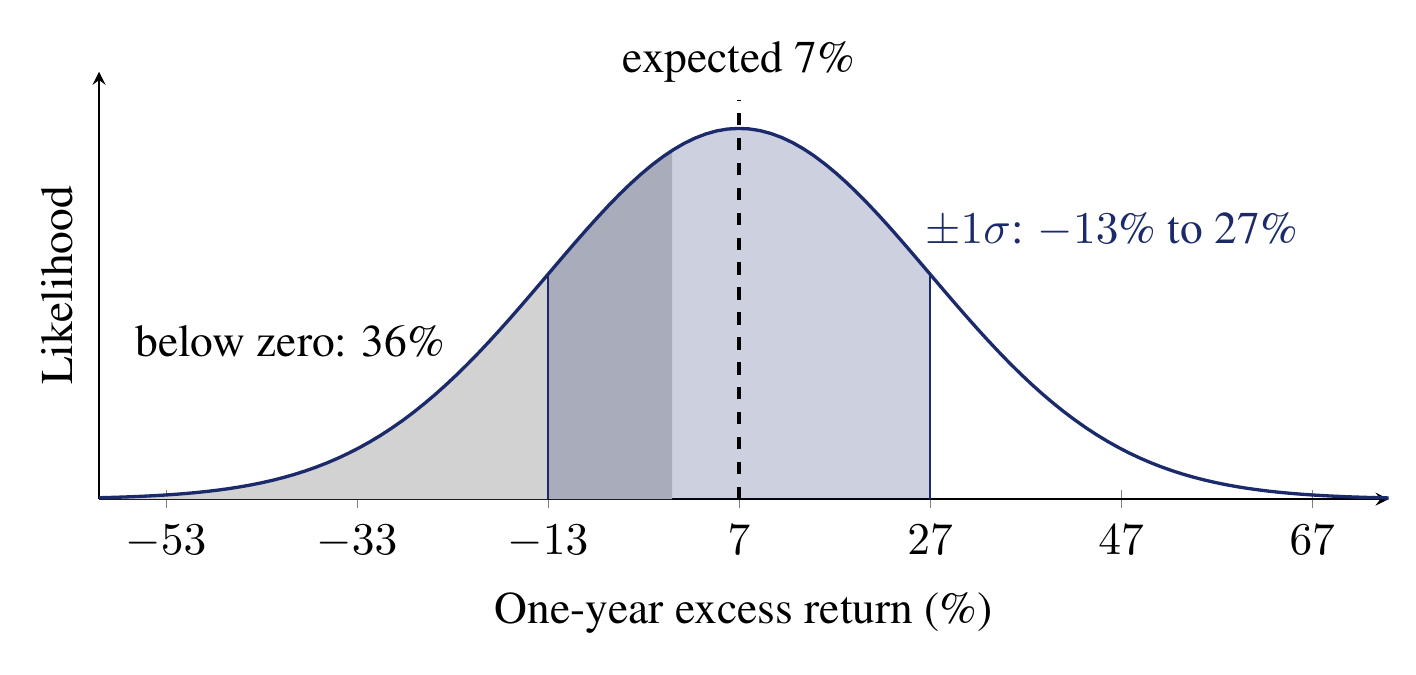
\includegraphics[width=0.85\linewidth]{images/fig01-1-one-year-return.png}
%\caption{One year's excess return on the stock market, assuming an expected excess return of 7\% and volatility of 20\%. The blue band covers the middle two-thirds of years, from $-13$\% to 27\%; the gray area is the 36\% of years with a negative excess return.}
%\label{fig:01-oneyear}
%\end{figure}


\textbf{The Sharpe ratio.} Sharpe (1966) proposed judging an investment by its excess return per unit of risk:
\begin{equation}
  \mathrm{SR} = \frac{E[R] - r_f}{\sigma}
  \label{eq:01-sr}
\end{equation}

The stock market's long-run Sharpe ratio is around 0.3 to 0.4 a year. Because leverage scales excess return and volatility equally, the Sharpe ratio does not change when a portfolio is levered up or down, which makes it the natural measure for comparing strategies (Figure~\ref{fig:01-sharpe-slope}).

\begin{figure}[htbp]
\centering
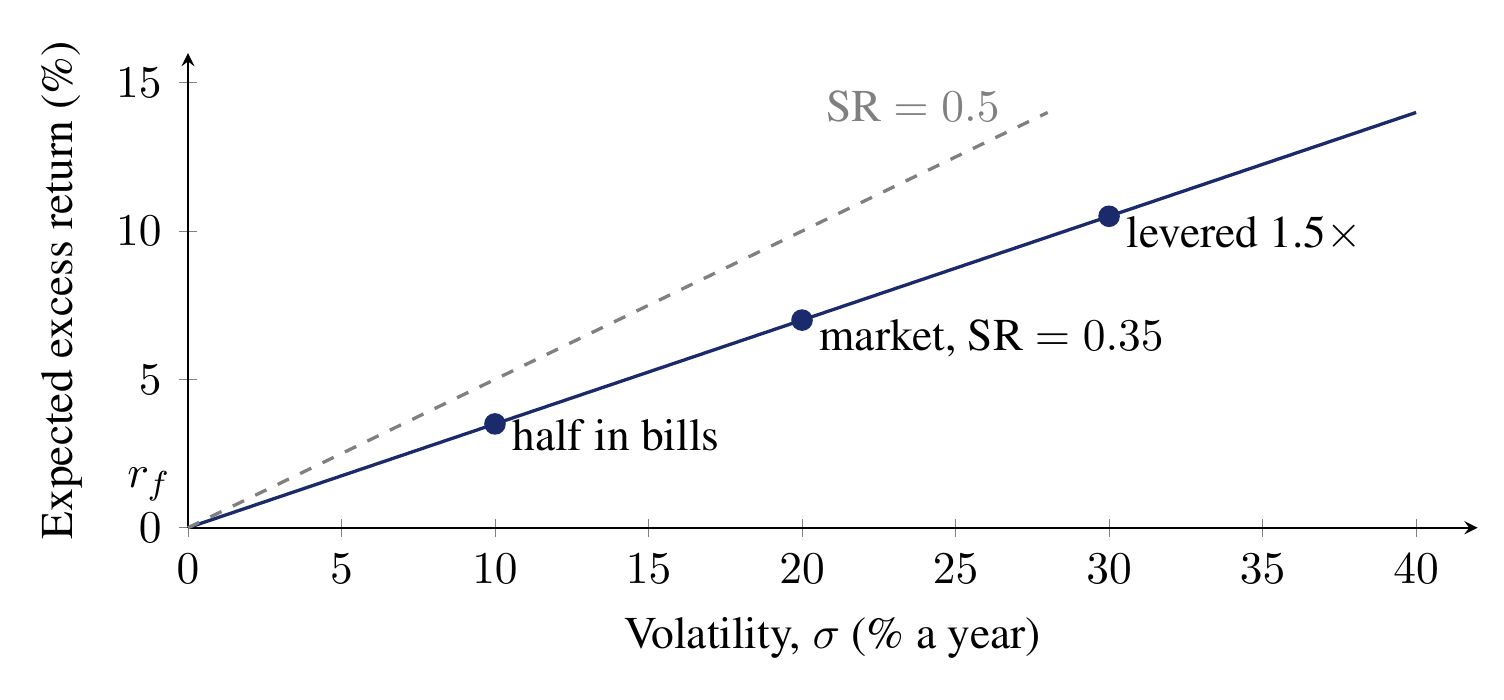
\includegraphics[width=0.85\linewidth]{images/fig01-2-sharpe-slope.png}
\caption{The Sharpe ratio is the slope of a line from the risk-free rate. Leverage moves a portfolio along its line, raising or lowering both excess return and volatility, but does not change the slope. A better strategy lies on a steeper line.}
\label{fig:01-sharpe-slope}
\end{figure}


\textbf{Risk, luck and skill.} Investors who make money in the stock market can do so for three different reasons. The distinction runs through the whole book.


\begin{itemize}
  \item \textbf{Bearing risk.} Stocks are riskier than Treasury bills, so over
  time they have paid more: this extra return is the equity premium defined
  above. An investor who simply buys and holds an index fund earns it without
  any special ability. Profit from bearing risk is a reward for risk, not
  evidence of skill.

  \emph{Examples.} (i) A retiree who has held an S\&P~500 index fund since
  1990 has earned far more than a savings account would have paid, without
  ever picking a stock. (ii) A manager who borrows to hold the index at
  1.5 times exposure beats the index in most years, but only because he
  carries 1.5 times its risk; in a crash he loses 1.5 times as much.
  (iii) A trader who sells out-of-the-money put options collects a small,
  steady premium month after month and looks like a genius, until a market
  crash wipes out years of gains. In each case the extra return is payment
  for risk that anyone could have taken.

  \item \textbf{Luck.} Returns are noisy, so some investors do well by
  chance, sometimes for years at a time. We also hear more about the winners
  than the losers, which makes luck look more common than it is.

  \emph{Examples.} (i) Ten thousand people each flip a coin every year to
  decide whether to hold stocks or cash. After ten years, about ten of them
  will have called the market right every single year, and some will write
  books about their method. (ii) A newsletter sends 1{,}000 readers a
  ``buy'' call on a stock and another 1{,}000 a ``sell'' call. Whichever way
  the stock moves, half the readers now hold a correct prediction, and the
  trick can be repeated on that half. (iii) An investor puts her savings into
  one small biotech company just before it receives surprise drug approval.
  The outcome was real; the evidence of ability is one draw.

  \item \textbf{Skill.} It is the ability to earn more than the
  risk taken explains: a return that a simple, cheap alternative carrying the
  same risk would not have delivered. Skill comes from better information,
  better analysis or better execution.

  \emph{Examples.} (i) \emph{Better information:} an analyst counts cars in
  retailers' parking lots from satellite images and forecasts sales before
  the companies report them. (ii) \emph{Better analysis:} a fund beats a
  portfolio with the same market, size and value exposures, after fees, over
  twenty years and across many independent bets. (iii) \emph{Better
  execution:} a trading firm buys and sells the same stocks as everyone else
  but pays less in trading costs and price impact, keeping a few basis points
  per trade that others give away.
\end{itemize}

\noindent\textbf{Exercise: which one is it?} Suppose an investor
consistently chooses the right stock at the right time. Before calling this
skill, ask two questions. First, \emph{does the risk explain it?} If the
investor's picks are mostly high-risk stocks bought during a rising market,
a cheap fund holding equally risky stocks might have done just as well, and
the profit is a reward for risk. Second, \emph{does luck explain it?} If the
record is short, or the investor is one of many whose picks we never hear
about, a run of good calls is what chance alone would produce. Only when the
answer to both questions is no does skill become the likely explanation. The
rest of this section shows how finance measures it.

Finance measures skill with \textbf{alpha}. Regress a strategy's excess return on the market's excess return:
\begin{equation}
  R_s - r_f = \alpha + \beta\,(R_m - r_f) + \varepsilon \nonumber
\end{equation}
where $R_s$ is the strategy's return, $R_m$ the market's return and $\varepsilon$ the part of the return the regression does not explain. The coefficient $\beta$ (\textbf{beta}) measures how much market risk the strategy carries, so $\beta\,(R_m - r_f)$ is the return that market exposure alone would have delivered. The intercept $\alpha$ is what is left over: the average return beyond what the strategy's market risk explains. For example, suppose a strategy has a beta of 0.6 and earns an average excess return of 6\% a year while the market earns 8\%. Market risk explains $0.6 \times 8 = 4.8$\%, so the strategy's alpha is $6 - 4.8 = 1.2$\% a year. Chapter 3 develops this regression and its extensions to other sources of risk.

A positive alpha is necessary for skill but not sufficient, because luck also produces positive alphas. Telling the two apart is the central problem of this chapter.

\textbf{Estimating a mean, and how uncertain the estimate is.} Given $T$ observations of a return with standard deviation $\sigma$, the sample mean has a \textbf{standard error} of $\sigma/\sqrt{T}$. The \textbf{t-statistic} of a mean is the estimate divided by its standard error; under the hypothesis that the true mean is zero, it has approximately a standard normal distribution, so values beyond about $\pm 1.96$ occur by chance only 5\% of the time. Applied to the Sharpe ratio, the same arithmetic gives a useful rule: the t-statistic of a strategy's mean return is approximately its annual Sharpe ratio times the square root of the number of years. A Sharpe ratio of 0.5 needs about 15 years of data to reach $t = 1.96$ (Figure~\ref{fig:01-years}).

\begin{figure}[htbp]
\centering
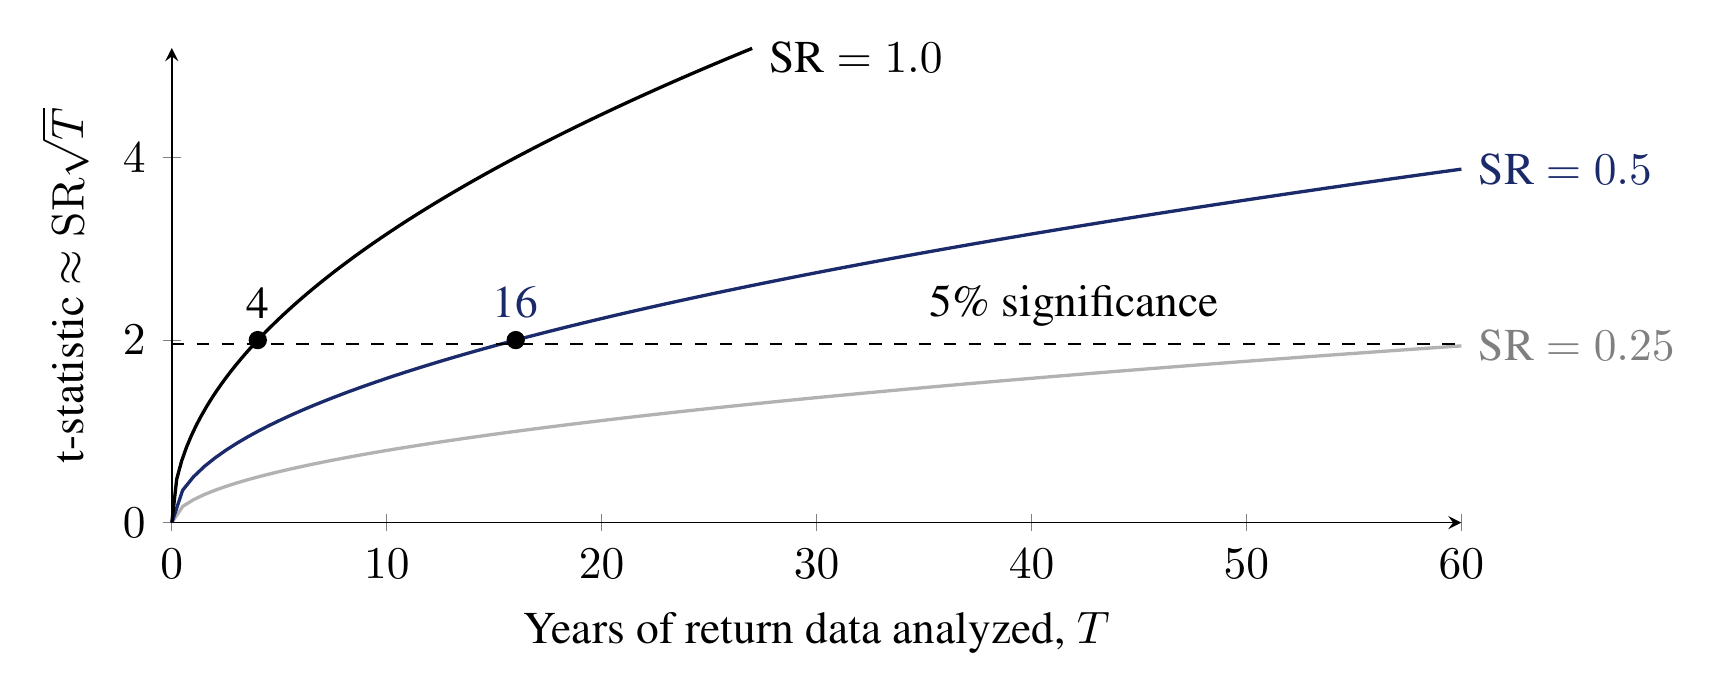
\includegraphics[width=0.85\linewidth]{images/fig01-3-years-needed.png}
\caption{How many years of return data are needed before a strategy's track record becomes statistically significant. The years count the length of the history being analyzed, not how long the strategy must trade or hold its positions. With a true Sharpe ratio of 0.5, about 15 years of data are needed to reach $t = 1.96$; with 0.25, about 61.}
\label{fig:01-years}
\end{figure}


\textbf{Worked example.} A strategy earns an average excess return of 0.5\% a month with a monthly standard deviation of 4\% over 10 years. Its annual mean is 6\%, its annual volatility 4\% $\times \sqrt{12} \approx 13.9$\%, and its Sharpe ratio $6/13.9 \approx 0.43$. The t-statistic is $0.5 / (4/\sqrt{120}) \approx 1.37$, not significant at 5\%, even though the strategy may be genuinely good.

\textbf{Further reading.} Bodie, Kane and Marcus, \emph{Investments}, chapters on risk, return and the historical record; Campbell, Lo and MacKinlay, \emph{The Econometrics of Financial Markets}, chapter 1 on returns; Cochrane, \emph{Asset Pricing}, for the theory of why expected returns differ.


\section{Efficient markets and the random walk}
\label{sec:01-efficient-markets}

The starting point for any claim about beating the market is the efficient market hypothesis. In Eugene Fama's (1970) formulation, a market is efficient if prices fully reflect available information. The intuition is competitive: if a predictable profit existed, traders would act on it, and their trading would push prices until the profit disappeared.

Fama distinguished three versions by the information set:

\begin{center}
\small
\begin{tabularx}{0.9\linewidth}{@{}>{\raggedright\arraybackslash}p{0.180\linewidth}>{\raggedright\arraybackslash}p{0.234\linewidth}>{\raggedright\arraybackslash}X@{}}
\toprule
Version & Prices reflect & Implication if true \\
\midrule
Weak form & Past prices and trading volume & Technical trading rules cannot earn abnormal returns \\
Semi-strong form & All public information & Analysis of public news and accounting data cannot earn abnormal returns \\
Strong form & All information, including private & Even insiders cannot earn abnormal returns \\
\bottomrule
\end{tabularx}
\end{center}

Few economists believe the strong form, and insider-trading laws exist because it fails. The weak and semi-strong forms are where the empirical debate happens, and where most claims in this book live.

\textbf{What efficiency does not imply.} Efficiency is often misread, so three clarifications matter:

\begin{enumerate}
  \item \textbf{It does not mean returns are unpredictable in every sense.} Expected returns can vary over time or across stocks as compensation for risk. A predictable return that is fair payment for risk is consistent with efficiency; a predictable return that is a free lunch is not. Separating the two is the joint-hypothesis problem: every test of efficiency is also a test of a model of what returns \emph{should} be.
  \item \textbf{It does not mean prices are always right.} It means mispricings are hard to identify and profit from after costs. Grossman and Stiglitz (1980) showed that a perfectly efficient market is impossible: if prices reflected everything, no one would pay to gather information. Markets must be inefficient enough to reward the people who make them efficient.
  \item \textbf{It does not mean volatility is unpredictable.} As Chapter 11 shows, risk is far more predictable than return.
\end{enumerate}

\textbf{The random walk as a benchmark.} If prices respond only to new, unpredictable information, price changes should look approximately like a random walk: tomorrow's change is unrelated to today's. Samuelson (1965) showed that properly anticipated prices fluctuate randomly. Lo and MacKinlay (1988) later rejected a strict random walk for weekly U.S. returns, so the model is not literally true. But it remains the right benchmark: any strategy must beat what a random walk, or a simple buy-and-hold position, would deliver.

For this book, the practical lesson is a prior. Before seeing evidence, a claim that a simple rule beats the market should be treated as unlikely. Not impossible, since the following chapters find some that survive, but unlikely enough to demand strong evidence.

\section{Signal and noise}
\label{sec:01-signal-noise}

The deeper reason claims are hard to verify is statistical: in finance, the signal is small and the noise is large. The differences between good and bad strategies are a few percent a year in expected return, while their returns move by fifteen or twenty percent a year at random.

\textbf{The Sharpe ratio, again.} The yardstick for a strategy is the Sharpe ratio of Equation~\eqref{eq:01-sr}. In this section we write $\mu$ for the strategy's expected return $E[R]$, so that $\mathrm{SR} = (\mu - r_f)/\sigma$, with all quantities annualized. Against the stock market's long-run Sharpe ratio of 0.3 to 0.4 (Section~\ref{sec:01-foundations}), a strategy with a true Sharpe ratio of 0.5 after costs would be a valuable discovery, and 1.0 would be exceptional.

\textbf{How precisely can we measure it?} With $T$ years of independent returns, the t-statistic for testing whether the true Sharpe ratio is zero is approximately
\begin{equation}
  t \approx \mathrm{SR}\,\sqrt{T}
  \label{eq:01-t}
\end{equation}
Equation~\eqref{eq:01-t} follows from the definition of the Sharpe ratio in Equation~\eqref{eq:01-sr} in four steps.

\begin{enumerate}
  \item \textbf{Estimate the mean.} Take $T$ years of annual excess returns. Their sample average, $\bar{x}$, is our estimate of the expected excess return $\mu - r_f$.
  \item \textbf{Find its standard error.} If the yearly returns are independent with volatility $\sigma$, the standard error of an average of $T$ of them is
  \begin{equation}
    \mathrm{SE}(\bar{x}) = \frac{\sigma}{\sqrt{T}} \nonumber
  \end{equation}
  \item \textbf{Form the t-statistic.} To test whether the true mean is zero, divide the estimate by its standard error:
  \begin{equation}
    t = \frac{\bar{x}}{\sigma/\sqrt{T}} = \frac{\bar{x}}{\sigma}\,\sqrt{T} \nonumber
  \end{equation}
  \item \textbf{Recognize the Sharpe ratio.} The ratio $\bar{x}/\sigma$ is the measured Sharpe ratio. Replacing $\bar{x}$ with the true mean $\mu - r_f$ gives the t-statistic we should expect on average:
  \begin{equation}
    t \approx \frac{\mu - r_f}{\sigma}\,\sqrt{T} = \mathrm{SR}\,\sqrt{T} \nonumber
  \end{equation}
  The result is approximate for two reasons: the measured mean differs from the true one, and in practice $\sigma$ must be estimated as well.
\end{enumerate}

The answer is the same with monthly or daily data. Sampling $k$ times a year gives $kT$ observations, each with mean $(\mu - r_f)/k$ and volatility $\sigma/\sqrt{k}$, so
\begin{equation}
  t = \frac{(\mu - r_f)/k}{(\sigma/\sqrt{k})/\sqrt{kT}} = \frac{\mu - r_f}{\sigma}\,\sqrt{T} \nonumber
\end{equation}
and the sampling frequency $k$ cancels.

By the same reasoning, the standard error of an estimated annual Sharpe ratio is roughly $1/\sqrt{T}$. Lo (2002) gives the refinements for non-normal and autocorrelated returns; the rough version is enough to see the problem. Setting $t = 1.96$, the usual 5\% significance threshold, in Equation~\eqref{eq:01-t} and solving for $T$ gives the number of years needed before a strategy's record can be distinguished from luck. Dividing both sides by SR gives $\sqrt{T} \approx 1.96/\mathrm{SR}$, and squaring gives
\begin{equation}
  T \approx \left(\frac{1.96}{\mathrm{SR}}\right)^2
  \label{eq:01-T}
\end{equation}

\begin{center}
\small
\begin{tabular}{@{}ll@{}}
\toprule
True Sharpe ratio & Years of data needed for $t = 1.96$ \\
\midrule
0.25 & 61 \\
0.50 & 15 \\
0.75 & 7 \\
1.00 & 4 \\
1.50 & 2 \\
\bottomrule
\end{tabular}
\end{center}

A strategy as good as the stock market itself needs more than two decades of data before its record is statistically convincing. Most fund track records, and most backtests shown to investors, are far shorter.

\textbf{Does the return frequency matter?} For the years-needed table above, no. Daily data give 252 observations a year instead of 12, but each daily return carries proportionally less information about the mean, so the years needed are the same. Table~\ref{tab:01-frequency} shows this for one strategy, with an expected excess return of 10\% a year, volatility of 20\% and so a Sharpe ratio of 0.5, observed over the same 16 years at three frequencies. The t-statistic is always the Sharpe ratio \emph{per period} times the square root of the \emph{number of periods}. Sampling more often multiplies the number of observations, but shrinks the Sharpe ratio of each one by the square root of that factor, and the two effects cancel.

\begin{table}[htbp]
\centering
\small
\caption{The same 16-year record measured annually, monthly and daily. Expected excess return 10\% and volatility 20\% a year, so the annual Sharpe ratio is 0.5. Daily figures assume 252 trading days a year.}
\label{tab:01-frequency}
\begin{tabular}{@{}lrrrrrr@{}}
\toprule
Frequency & Observations & Mean per & Volatility per & Sharpe ratio & $\sqrt{N}$ & $t$ \\
 & $N$ & period (\%) & period (\%) & per period & & \\
\midrule
Annual  & 16    & 10.000 & 20.00 & 0.500  & 4.00  & 2.00 \\
Monthly & 192   & 0.833  & 5.77  & 0.144  & 13.86 & 2.00 \\
Daily   & 4{,}032 & 0.040 & 1.26  & 0.0315 & 63.50 & 2.00 \\
\bottomrule
\end{tabular}
\end{table}

Going from annual to monthly data gives 12 times as many observations, but each has a mean 12 times smaller and a volatility $\sqrt{12}$ times smaller, so its Sharpe ratio is $\sqrt{12}$ times smaller. Since $\sqrt{N}$ grows by exactly $\sqrt{12}$, the t-statistic does not change. The same happens with 252 in place of 12 for daily data. This is why Equation~\eqref{eq:01-t} can be stated in years: $T$ is the number of observations only when the Sharpe ratio is measured over the same period, and for an annual Sharpe ratio that period is a year. Merton (1980) made this point: the precision of an estimated expected return depends on the length of the history, not on the sampling frequency. With log returns the reason is especially plain. The average annual log return over $T$ years depends only on the first and last prices,
\begin{equation}
  \bar{r} = \frac{\ln P_T - \ln P_0}{T}, \nonumber
\end{equation}
because every price in between is added once and subtracted once. Dividing a century into days rather than months adds no information about the mean, and its standard error stays at about $20/\sqrt{100} = 2$\%, as in Section~\ref{sec:01-foundations}. The same holds for every claim about \emph{average} returns, such as the equity premium, value, momentum and published anomalies, which is why Chapters 7 to 10 can test them on monthly data without losing anything.

Claims about \emph{risk} are different. Each additional observation adds information about how much returns vary, so the precision of an estimated volatility grows with the number of returns $N$, not just the number of years:
\begin{equation}
  \mathrm{SE}(\hat{\sigma}) \approx \frac{\sigma}{\sqrt{2N}} \nonumber
\end{equation}
With 20\% volatility and a century of data, the standard error is about 0.41 percentage points with monthly returns ($N = 1{,}200$) and about 0.09 with daily returns ($N \approx 25{,}200$), more than four times smaller. This is why the chapters on volatility (Chapter 11), value at risk (Chapter 13), delta hedging (Chapter 15) and trading costs (Chapter 6) use daily or even intraday data.

The rule ``the mean needs a long history, risk needs frequent data'' is a good guide, but it has limits.
\begin{itemize}
  \item \textbf{Very high frequency adds noise.} At intraday frequencies, the bounce between bid and ask prices and stale quotes distort measured returns, so for volatility, more frequent data help only up to a point.
  \item \textbf{Daily betas can be biased.} Stocks that trade infrequently react to market news with a delay, which makes their daily betas too low. Monthly data, or a correction that adds lagged market returns to the regression (Dimson, 1979), reduces the bias. This matters for the low-risk anomaly in Chapter 12.
  \item \textbf{Annualizing is not automatic.} The rules in Section~\ref{sec:01-foundations} for converting monthly figures to annual ones assume that returns are uncorrelated over time. When they are autocorrelated, as for many hedge funds and illiquid assets, a monthly Sharpe ratio multiplied by $\sqrt{12}$ can be badly off (Lo, 2002).
  \item \textbf{The cancellation is exact only for log returns.} For simple returns, the precision of the mean still depends mainly on the length of the history, but only approximately.
\end{itemize}

The practical lesson is to match the data to the claim. To measure an expected return more precisely, you need a longer history, not more frequent data; to measure risk, more frequent data help.

\textbf{What a ten-year record can tell you.} The ``10 years'' here is not how long the strategy holds its positions; the strategy may trade daily or monthly. It is the length of the track record you look at when you judge the strategy. A thought experiment shows how noisy that judgment is.

\begin{enumerate}
  \item \textbf{The strategy is genuinely good.} Suppose its true Sharpe ratio is 0.5. Nobody can see this number directly; we see only the Sharpe ratio measured from its realized returns.
  \item \textbf{The measurement is noisy.} With a 10-year record, the standard error of the measured Sharpe ratio is about $1/\sqrt{10} \approx 0.32$.
  \item \textbf{The record could show almost anything.} A 95\% range for the measured Sharpe ratio is $0.5 \pm 1.96 \times 0.32$, or about $-0.1$ to 1.1. Imagine watching the same strategy over many different decades. In one decade it looks like a star, with a Sharpe ratio near 1.0; in another it looks like a failure, near zero. The strategy is the same; only the decade differs.
  \item \textbf{Luck can look like skill.} A strategy with no skill has a true Sharpe ratio of zero, yet its measured Sharpe ratio exceeds 0.5 whenever the noise is more than $0.5/0.32 \approx 1.6$ standard errors. That happens in roughly 6\% of decades, by luck alone.
\end{enumerate}

Figure~\ref{fig:01-ten-year} draws the two cases side by side. The curves overlap heavily: a measured Sharpe ratio of 0.4, for example, is quite consistent with both a genuinely good strategy and a useless one. A ten-year record cannot reliably tell them apart.

\begin{figure}[htbp]
\centering
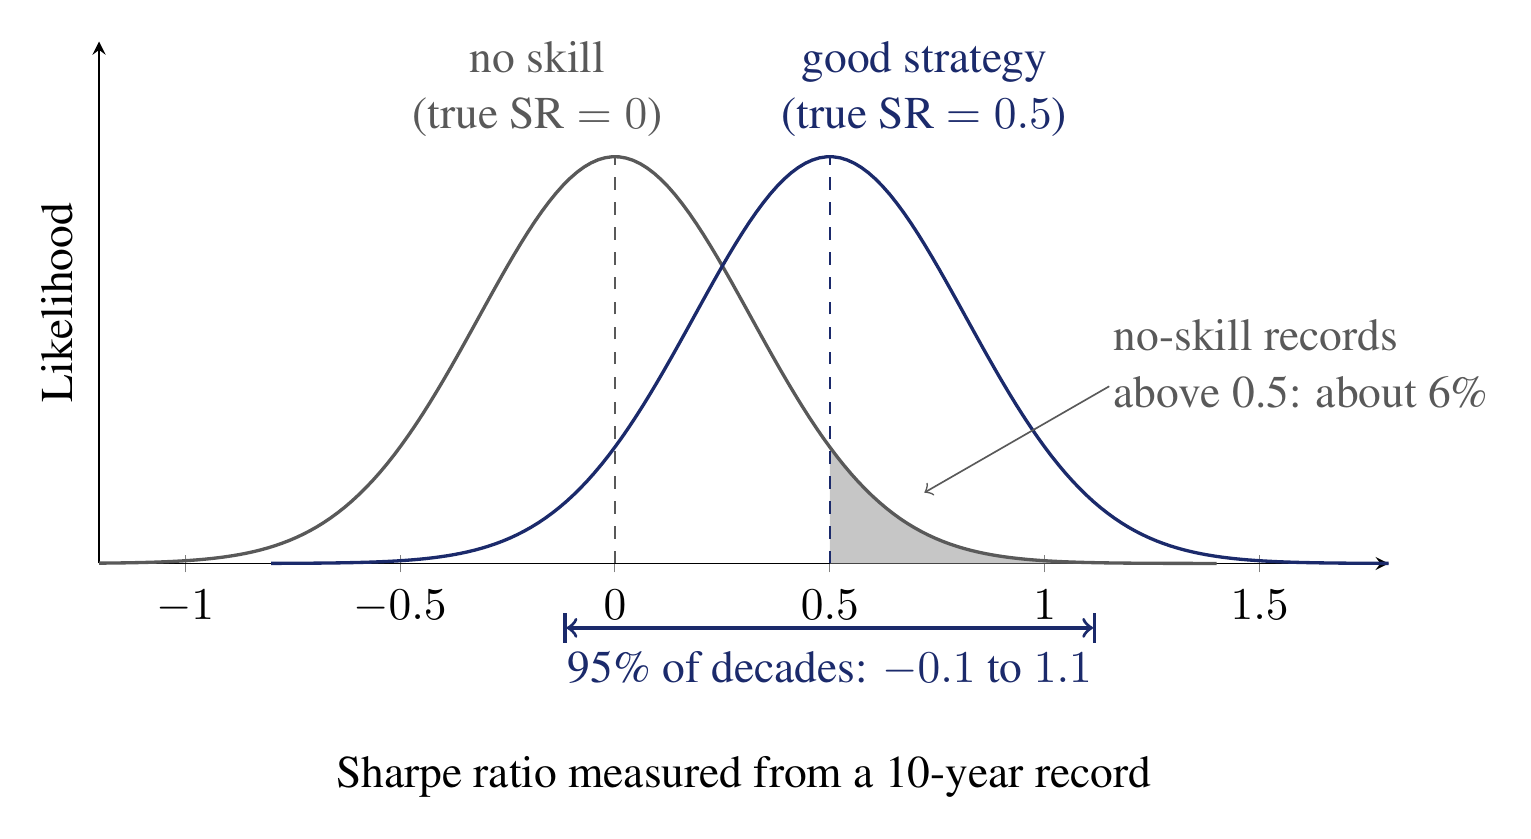
\includegraphics[width=0.85\linewidth]{images/fig01-4-ten-year-record.png}
\caption{What a 10-year record can show. The gray curve is the range of Sharpe ratios a strategy with no skill produces over different decades; the blue curve is the same for a strategy with a true Sharpe ratio of 0.5. The shaded tail is the 6\% of decades in which the useless strategy beats 0.5 by luck.}
\label{fig:01-ten-year}
\end{figure}

\textbf{Why prediction is harder than it looks.} The same arithmetic applies to forecasting. A model that explains just 1\% of the variation in monthly returns would be worth a great deal to an investor (Campbell and Thompson 2008 make this point). But an $R^2$ of 1\% is almost impossible to distinguish from zero in a few decades of data, and almost trivially easy to produce by accident when many models are tried. Small true effects, large noise and short samples together make finance a field where false discoveries are easy and true ones are hard to confirm.

\section{Cautions: Why backtests can mislead}
\label{sec:01-backtests}

A backtest applies a strategy's rules to historical data to show how it would have performed. It is the most common evidence offered for a strategy and the easiest to get wrong. Seven problems account for most misleading backtests; later chapters treat each in depth.

\begin{enumerate}
  \item \textbf{Selection across many trials.} If you test 100 rules and report the best, its record overstates what it will deliver. This is the subject of the lab, and of Chapter 4.
  \item \textbf{Overfitting parameters.} Tuning a rule's settings (a 47-day average instead of 50, a threshold of 1.3 instead of 1.5) fits the noise in the sample. Each added parameter is another hidden trial.
  \item \textbf{Look-ahead bias.} Using information that was not available at the time, such as revised economic data or accounting figures before their release date (Chapter 2).
  \item \textbf{Survivorship bias.} Testing only on companies or funds that still exist, which excludes the failures (Chapter 2).
  \item \textbf{Ignoring costs.} Spreads, commissions, market impact, borrowing fees and taxes can erase a paper profit, especially for high-turnover strategies (Chapter 6).
  \item \textbf{Short or unrepresentative samples.} A decade of data may contain only one market regime. As Section~\ref{sec:01-signal-noise} showed, a short sample cannot separate skill from luck.
  \item \textbf{A story told after the fact.} Once a pattern is found, a plausible explanation is easy to write. The story makes the result feel robust, but it was written to fit the data, not tested against it.
\end{enumerate}

These problems compound. A backtest can be honest in every visible detail, using correct prices, real costs and no look-ahead, and still mislead because it is the best of many attempts that are never shown.

\begin{callout}
\textbf{What Failed: butter in Bangladesh.} To show how easy data mining is, David Leinweber searched a United Nations database for series that tracked the S\&P 500. Butter production in Bangladesh fit well; adding U.S. cheese production and the sheep population of Bangladesh and the United States raised the fit further, with an $R^2$ that looked like a breakthrough. The relationship, of course, predicted nothing afterward. The example was a joke with a serious point: search enough series, and a near-perfect fit is guaranteed. Leinweber later wrote it up as ``Stupid Data Miner Tricks'' (2007).
\end{callout}

\section{The claims-on-trial method and the verdict scale}
\label{sec:01-method}

Every claim chapter and every lab opens with a line labelled \textbf{Claim on trial}. The label is a reminder of who does the work: you are not told whether the claim is true, you test it. The book's subtitle, \emph{Active Learning by Verifying Famous Claims}, describes the bargain. Each trial needs a method (a regression, a backtest, a volatility model, a hedge), and you learn that method in order to reach a verdict, then use it again in later trials until it is second nature.

The rest of this book applies one method to every claim. It is simple enough to remember and strict enough to protect against the problems in Section~\ref{sec:01-backtests}.

\begin{enumerate}
  \item \textbf{Claim} --- State what is asserted in one testable sentence. ``Momentum works'' is vague; ``stocks with the highest 12-month returns, skipping the last month, outperform the lowest by a positive average return after costs'' can be tested.
  \item \textbf{Understand} --- Learn how the idea works and how the original evidence was produced: the data, sample period, method and number of alternatives the authors tried.
  \item \textbf{Verify} --- Rebuild the result yourself, then stress-test it: out of sample, in other markets, after costs, after publication.
  \item \textbf{Judge} --- Reach a verdict on the scale below, dated with the sample period tested.
  \item \textbf{Apply} --- State what an investor or practitioner can actually use, and what remains open.
\end{enumerate}

\textbf{The verdict scale}

\begin{center}
\small
\begin{tabularx}{0.9\linewidth}{@{}>{\raggedright\arraybackslash}p{0.162\linewidth}>{\raggedright\arraybackslash}X@{}}
\toprule
Verdict & Meaning \\
\midrule
Survives & The result replicates, holds out of sample and in other markets, and remains economically meaningful after costs. \\
Weakens & The result is real but smaller, less reliable, or narrower than claimed, for example only in small stocks or before publication. \\
Fails & The result does not replicate, or disappears out of sample or after costs. \\
Provisional & The evidence is too new or too mixed for a firm verdict. \\
\bottomrule
\end{tabularx}
\end{center}

Two habits make the method work. First, \textbf{decide the test before seeing the result}: write down the claim, the data and the pass criteria first, so the test cannot be bent to fit the outcome. Second, \textbf{always ask ``compared to what?''}: every claim is judged against a simple benchmark, such as the market, the historical average or a naive rule, never against zero.

This chapter's lab applies the method to a claim at the root of the whole field: whether a track record can reveal real skill.

\section{Lab 1: Brilliant by chance}
\label{sec:01-lab}

\begin{callout}
\textbf{Lab 1 at a glance.} Claim on trial: a long enough track record can reveal real skill. Data: monthly U.S. market excess returns and Treasury bill rates since 1926, from the Kenneth R. French Data Library (downloaded automatically). Tools: Python with pandas, NumPy and matplotlib, plus the book's fintest module. Time: about one hour, including the guided notebook; the code itself runs in seconds. Code: repository folder \texttt{ch01-brilliant-by-chance/}.
\end{callout}

\subsection*{Design}

The lab answers the claim by first measuring what luck alone can do. It builds strategies whose skill we know for certain: none. Whatever these strategies achieve sets the bar that a real strategy's record must clear. Each of 1,000 strategies is, every month, either invested in the stock market or holding Treasury bills. It switches between the two at random, with an average holding period between 3 and 24 months, so the strategies look like real market-timing rules. They use no information at all, and each month's position is fixed before that month's return is known. The design follows the logic of Bailey, Borwein, L\'opez de Prado and Zhu (2014), who show that the best of many backtests can look impressive by chance alone, and of Harvey, Liu and Zhu (2016), who argue that the usual $t > 2$ hurdle is far too low when many strategies are tried.

The sample is split in two. The first half, roughly 1926 to 1975, plays the role of the \textbf{backtest}: the period in which a researcher would test the strategies and choose the best. The second half, roughly 1976 to today, is the period \textbf{after selection}: what an investor who adopted the chosen strategy would have experienced.

\textbf{Measuring skill.} A strategy that is in the market part of the time will earn part of the market's return with no skill at all. Skill is therefore measured as \textbf{alpha against buy-and-hold} (Section~\ref{sec:01-foundations}): the intercept in a regression of the strategy's excess return on the market's excess return. For every strategy in this lab, the true alpha is zero. Each alpha is tested with a t-statistic using Newey--West standard errors, which Chapter 3 explains.

\subsection*{Three parts}

\begin{enumerate}
  \item \textbf{Signal and noise.} Measure the market's Sharpe ratio over the full sample and over every 10-year window, and compute how many years are needed to detect a given Sharpe ratio (Figure 1.5 and the table in Section~\ref{sec:01-signal-noise}).
  \item \textbf{Brilliant by chance.} Backtest the 1,000 random strategies, count how many look significant, pick the best, and follow all of them into the period after selection (Figures 1.6 to 1.8).
  \item \textbf{The cost of searching.} Show how the best backtest t-statistic rises as more strategies are tried, from 1 to 1,000 (Figure 1.9).
\end{enumerate}

\subsection*{What theory predicts}

Because every strategy has zero skill, statistics tells us in advance roughly what to expect, which makes the lab a test of your intuition:

\begin{center}
\small
\begin{tabularx}{0.9\linewidth}{@{}>{\raggedright\arraybackslash}p{0.450\linewidth}>{\raggedright\arraybackslash}X@{}}
\toprule
Measure & Expected for 1,000 zero-skill strategies \\
\midrule
Strategies passing $t > 1.96$ in the backtest & About 25 (2.5\%), typically between about 15 and 50 \\
Best backtest t-statistic & About 3.2 \\
Threshold that controls false discoveries across all 1,000 (Bonferroni, 5\%) & $t > 3.89$ \\
Correlation between backtest and later t-statistics & About zero \\
Average later t-statistic of the backtest ``winners'' & About zero \\
\bottomrule
\end{tabularx}
\end{center}

The count of significant strategies varies more than a simple coin-flip model suggests, for two reasons the lab asks readers to explain: all 1,000 strategies share one market history, and heavy-tailed returns make standard errors slightly too small.

\subsection*{What readers will see}

The chapter presents five exhibits. Figure 1.5 tracks the market's 10-year Sharpe ratio. Figure 1.6 shows the 1,000 backtest t-statistics against the bell curve that pure luck predicts. Figure 1.7 plots the growth of \$1 in the best random strategy against the market, with the backtest and after-selection periods marked. Figure 1.8 plots each strategy's backtest t-statistic against its later t-statistic. Figure 1.9 shows how the best backtest improves with the number of strategies tried.

\emph{[Draft note: the figures and numbers are generated by running the lab on the Kenneth French data at the time of publication. The book prints the real-data results; the text above does not anticipate them beyond what statistical theory predicts.]}

\subsection*{Your verdict}

The lab ends by asking readers to write their own verdict on the claim in two or three sentences, using their numbers. The expected conclusion is \textbf{survives, with conditions}. A track record can reveal real skill, but only when three conditions hold:

\begin{enumerate}
  \item \textbf{It is long enough for its Sharpe ratio.} About $(1.96/\mathrm{SR})^2$ years: roughly 15 for a Sharpe ratio of 0.5 and 4 for 1.0 (Section~\ref{sec:01-signal-noise}).
  \item \textbf{It clears a bar that allows for how many strategies were tried.} After 1,000 tries, that bar is $t > 3.89$, not 1.96; the random strategies in Parts 2 and 3 show why.
  \item \textbf{It keeps working on data that played no part in choosing it}, such as the period after selection.
\end{enumerate}

A record that meets all three is real evidence of skill. A short record, or the best of many tries judged by the usual bar, is not.

\textbf{What the verdict means for you.} Profits can come from bearing risk, from luck or from skill (Section~\ref{sec:01-foundations}), and skill can be found. The conditions above are not obstacles; they are the specification a credible strategy must meet. Lab extension~9 lets you plant a genuinely skilled strategy among the 1,000 and see what it takes for it to stand out. The rest of the book gives you the tools to meet each condition, and later chapters find strategies whose alpha survives testing.

\section{What investors can use}
\label{sec:01-investors}

The practical lesson of this chapter is to judge evidence by \textbf{how it was produced}, not by how good it looks. A spectacular track record and a modest one can carry the same information, or none, depending on the search behind them. The same lesson tells you what a convincing record looks like: long enough for its Sharpe ratio, honest about the number of tries, and confirmed on new data.

\textbf{Rules of thumb}

\begin{enumerate}
  \item Treat any backtest as the best of many tries unless you are shown otherwise.
  \item Discount short records heavily. Under ten years, a record says little about skill, as Section~\ref{sec:01-signal-noise} showed.
  \item Prefer evidence from data that played no part in designing the strategy: the period after a paper's publication, after a fund's launch, or after a rule was fixed.
  \item Ask for the benchmark. A strategy's return means little until it is compared with what a simple alternative, such as an index fund, earned over the same period.
  \item Know what a convincing record needs: about 15 years for a Sharpe ratio of 0.5, a higher bar after a search, and results that hold after the strategy was fixed.
\end{enumerate}

\textbf{Questions to ask a fund manager or strategy vendor}

\begin{itemize}
  \item How many strategies or parameter settings did you test before choosing this one?
  \item Which part of this record is a live track record, and which part is a backtest?
  \item When was the strategy's design fixed, and how has it performed since then?
  \item What is the benchmark, and what is the strategy's alpha against it, with its t-statistic?
  \item What happened to the other strategies or funds you launched at the same time?
  \item Are transaction costs, fees and taxes included?
\end{itemize}

\section{Looking ahead}
\label{sec:01-ahead}

This chapter showed that prices are hard to predict, that the noise in returns hides real effects and manufactures false ones, and that selection turns luck into impressive backtests. The rest of the book builds on these points in three steps.

\textbf{Part I continues} with Chapter 2, on the data itself: how survivorship bias, look-ahead bias and micro-cap stocks inflate results before any statistics are run.

\textbf{Part II} turns the warnings of this chapter into tools: statistics built for noisy returns (Chapter 3), corrections for multiple testing such as the deflated Sharpe ratio (Chapter 4), honest out-of-sample design (Chapter 5) and transaction costs (Chapter 6).

\textbf{Parts III to VII} then put the field's most important claims on trial, from return predictability and the value premium to risk models, option hedging, bond, credit and currency markets, and machine learning. Each chapter ends with a verdict. Some claims survive. That is the point of the method: not to dismiss every finding, but to separate the ones that hold from the ones that only looked good.

\section*{Exercises}
\addcontentsline{toc}{section}{Exercises}

\subsection*{Conceptual (all readers)}

\begin{enumerate}
  \item Explain in your own words why a market in which prices fully reflected all information could not exist (Grossman and Stiglitz). What does this imply for anyone claiming to beat the market?
  \item A fund has returned 4\% a year more than its benchmark for five years, with a tracking error (volatility of the excess return) of 8\%. Compute the t-statistic of its excess return. Is the record evidence of skill?
  \item Using the formula in Section~\ref{sec:01-signal-noise}, how many years of data would you need to detect a strategy with a true Sharpe ratio of 0.3? What does your answer imply for most fund track records?
  \item A newsletter reports that its ``crash indicator'' correctly called the last three bear markets. List three questions you would ask before believing it.
  \item Pick a recent strategy, fund or AI-based product advertised online. Using the problems listed in Section~\ref{sec:01-backtests}, identify which ones could inflate its record, and write the first question you would ask.
\end{enumerate}

\subsection*{Lab extensions (technical readers)}

\begin{enumerate}
  \setcounter{enumi}{5}
  \item Re-run Lab 1 with five different seeds. Record the number of strategies with $t > 1.96$ and the best $t$ each time. How much do they vary, and why?
  \item Increase the number of strategies to 10,000. How large is the best backtest t-statistic? Compare it with Figure 1.9 and with the approximation $\sqrt{2 \ln N}$.
  \item Move the split between backtest and after-selection periods to 1990. Do the conclusions change?
  \item Add one ``needle'' strategy with genuine skill: in the market with probability 0.55 in months the market rises and 0.45 in months it falls. Where does it rank among the 1,000 in the backtest? What does that tell you about finding real skill among many tries?
  \item Replace the random strategies with 200 moving-average timing rules (different window lengths). Unlike the random strategies, these might contain real information. How would you decide whether the best rule's backtest shows skill? Write down your test before running it.
\end{enumerate}

\section*{References}
\addcontentsline{toc}{section}{References}

\begin{itemize}
  \item Bailey, D. H., Borwein, J. M., L\'opez de Prado, M. and Zhu, Q. J. (2014). Pseudo-Mathematics and Financial Charlatanism: The Effects of Backtest Overfitting on Out-of-Sample Performance. \emph{Notices of the American Mathematical Society} 61(5): 458--471.
  \item Campbell, J. Y. and Thompson, S. B. (2008). Predicting Excess Stock Returns Out of Sample: Can Anything Beat the Historical Average? \emph{Review of Financial Studies} 21(4): 1509--1531.
  \item Dimson, E. (1979). Risk Measurement When Shares Are Subject to Infrequent Trading. \emph{Journal of Financial Economics} 7(2): 197--226.
  \item Fama, E. F. (1970). Efficient Capital Markets: A Review of Theory and Empirical Work. \emph{Journal of Finance} 25(2): 383--417.
  \item Grossman, S. J. and Stiglitz, J. E. (1980). On the Impossibility of Informationally Efficient Markets. \emph{American Economic Review} 70(3): 393--408.
  \item Harvey, C. R., Liu, Y. and Zhu, H. (2016). \ldots and the Cross-Section of Expected Returns. \emph{Review of Financial Studies} 29(1): 5--68.
  \item Leinweber, D. J. (2007). Stupid Data Miner Tricks: Overfitting the S\&P 500. \emph{Journal of Investing} 16(1): 15--22.
  \item Lo, A. W. (2002). The Statistics of Sharpe Ratios. \emph{Financial Analysts Journal} 58(4): 36--52.
  \item Lo, A. W. and MacKinlay, A. C. (1988). Stock Market Prices Do Not Follow Random Walks: Evidence from a Simple Specification Test. \emph{Review of Financial Studies} 1(1): 41--66.
  \item Merton, R. C. (1980). On Estimating the Expected Return on the Market: An Exploratory Investigation. \emph{Journal of Financial Economics} 8(4): 323--361.
  \item Samuelson, P. A. (1965). Proof That Properly Anticipated Prices Fluctuate Randomly. \emph{Industrial Management Review} 6(2): 41--49.
  \item Sharpe, W. F. (1966). Mutual Fund Performance. \emph{Journal of Business} 39(1): 119--138.
\end{itemize}

\textbf{Data:} Kenneth R. French Data Library, Fama/French 3 Factors, monthly. \url{https://mba.tuck.dartmouth.edu/pages/faculty/ken.french/data_library.html}

% Chapter 2 -- Financial Data and How to Use It Well
% Requires: amsmath, amssymb, booktabs, array, tabularx, longtable, graphicx, tcolorbox (breakable, skins), hyperref or url.
% Defines the callout box only if the preamble has not.
\providecolor{fenavy}{HTML}{1B2A6B}
\providecolor{feshade}{HTML}{F3F5FA}
\makeatletter
\@ifundefined{callout}{%
  \newtcolorbox{callout}{breakable, enhanced,
    colback=white, colframe=gray!70, boxrule=0.5pt, arc=1mm,
    borderline west={2.5pt}{0pt}{gray!70},
    left=8pt, right=8pt, top=4pt, bottom=4pt}%
}{}
\makeatother

\chapter{Financial Data and How to Use It Well}
\label{ch:02}

Chapter~\ref{ch:01} showed what a track record must do to reveal real skill. This chapter turns to what comes first: the data the record is built on. A backtest can test a single idea with honest statistics and still give the wrong answer because of how its dataset was built. The good news is that each problem is well understood, and each has a fix.

The problems are rarely dramatic. Each looks like a technical detail, and each can add a percentage point or more a year to a strategy's measured return:

\begin{itemize}
  \item a price series that is not adjusted for stock splits and dividends, so ordinary corporate events look like gains or losses;
  \item a portfolio that gives a \$20 million company the same weight as a \$2 trillion one, so the result is driven by stocks almost no one can trade in size;
  \item a database that keeps only the companies that still exist, so the failures, and the losses they caused, are missing;
  \item an accounting number used months before it was published, so the strategy trades on information no investor had at the time;
  \item an average return quoted in a way that overstates what an investor actually earned.
\end{itemize}

The claim on trial in this chapter is the one every reader working with free data needs to be true: \textbf{free, public data can support a reliable backtest.} Every lab in this book relies on it, so we test it first, and the answer comes with a checklist that tells you exactly how to make it true.


By the end of the chapter you will be able to:

\begin{itemize}
  \item explain how stock splits and dividends change quoted prices, and why research uses adjusted prices;
  \item compute market capitalization and distinguish value-weighted, equal-weighted and price-weighted portfolios;
  \item describe the main research datasets and their free counterparts, and explain delisting returns and point-in-time data;
  \item choose the right return measure for each task (simple or log, price or total, raw or excess), and explain why arithmetic and geometric averages differ;
  \item recognize survivorship bias, look-ahead bias, micro-cap effects and data snooping, and estimate how much each can distort a result;
  \item apply a data checklist before trusting any backtest.
\end{itemize}

In the lab you will measure four of these problems with nearly a century of real market data and one controlled simulation, see how much each can inflate a strategy's apparent performance, and see how much each fix recovers.

\section{Foundations: where financial data comes from}
\label{sec:02-foundations}

\textbf{Prices, corporate actions and adjusted prices.} A stock's quoted price changes for reasons that are not gains or losses to shareholders. These events are called \textbf{corporate actions}. Two matter most.

\begin{itemize}
  \item \textbf{Stock split.} In a two-for-one split, each share becomes two and the price halves. A shareholder who owned one share at \$100 now owns two shares at \$50: still \$100 in total. A chart of the raw price would show a 50\% ``crash'' that never cost anyone a cent.
  \item \textbf{Dividend.} A dividend pays cash to shareholders. The share price typically falls by roughly the dividend on the \textbf{ex-dividend date}, the first day on which a buyer of the stock no longer receives the payment. If a \$100 stock pays a \$2 dividend and opens at \$98, the price return is $-2$\%, but the shareholder's total return is zero: \$98 in stock plus \$2 in cash.
\end{itemize}

Databases therefore publish \textbf{adjusted prices}, which rescale past prices so that the change in the adjusted price equals the shareholder's return. After the split above, for example, every earlier price is divided by two. Total-return series also adjust for dividends. Data vendors differ in how they adjust, which is one reason two sources can disagree about the same stock's history.

\textbf{Market capitalization and index weights.} A company's \textbf{market capitalization} (or market value) is its share price times the number of shares outstanding: one billion shares at \$50 is a \$50 billion company. How a portfolio uses this number decides which stocks drive its results.

\begin{itemize}
  \item A \textbf{value-weighted} (capitalization-weighted) portfolio holds each stock in proportion to its market capitalization. If company A is worth \$900 billion and company B is worth \$100 billion, together they are worth \$1 trillion, so A receives 90\% of the money invested and B receives 10\%.
  \item An \textbf{equal-weighted} portfolio gives each stock the same share of the money, whatever its size. With the same two companies, A and B each receive 50\%. Company B is only 10\% of the market's value but gets half the portfolio, so equal weighting gives small companies far more influence than their size in the economy.
  \item A \textbf{price-weighted} index, such as the Dow Jones Industrial Average, weights by share price alone. A \$500 stock counts ten times as much as a \$50 stock, whatever the size of the two companies. This is a historical convention with no economic rationale.
\end{itemize}

A value-weighted portfolio needs little rebalancing, because its weights move with prices automatically; it trades mainly when stocks enter or leave the portfolio or companies issue or buy back shares. An equal-weighted portfolio must be rebalanced regularly as prices drift apart, selling part of the stocks that have risen and buying more of those that have fallen to restore equal weights.


\textbf{The main research databases.} Most empirical finance rests on a handful of sources.

\begingroup
\small
\setlength{\LTpre}{6pt}\setlength{\LTpost}{6pt}
\begin{longtable}{@{}>{\raggedright\arraybackslash}p{0.2\linewidth}>{\raggedright\arraybackslash}p{0.42\linewidth}>{\raggedright\arraybackslash}p{0.22\linewidth}@{}}
\toprule
Source & What it holds & Access \\
\midrule
\endfirsthead
\multicolumn{3}{@{}l}{\emph{(continued)}}\\
\toprule
Source & What it holds & Access \\
\midrule
\endhead
\midrule
\multicolumn{3}{r@{}}{\emph{continued on next page}}\\
\endfoot
\bottomrule
\endlastfoot
CRSP (Center for Research in Security Prices) & Daily and monthly returns, prices, shares and delisting information for U.S. stocks since 1926, including companies that no longer exist & Subscription, usually through WRDS \\
Compustat & Company accounting data: balance sheets, income statements, cash flows & Subscription \\
Kenneth R. French Data Library & Factor returns and sorted portfolio returns built from CRSP and Compustat & Free \\
FRED (Federal Reserve Bank of St.\ Louis) & Interest rates, inflation, macroeconomic series; ALFRED holds earlier vintages & Free \\
Exchange and vendor feeds (Yahoo Finance and others) & Recent prices and adjusted prices for currently listed securities & Free or commercial; coverage and adjustment methods vary \\
\end{longtable}
\endgroup

WRDS (Wharton Research Data Services) is the platform through which most universities access CRSP and Compustat. A \textbf{factor} is the return on a portfolio built to capture one source of return, such as small minus large companies. A \textbf{vintage} is a dataset as it stood on a particular date, before later revisions. This book's labs use only free sources. Where a test needs data that only subscription databases hold, such as the returns of companies that delisted, the labs use simulations and say so.

\textbf{Delisting.} A company is \textbf{delisted} when its stock stops trading on an exchange. Companies leave through mergers, going private, moving exchanges or failure. The \textbf{delisting return} is the return from the last trading price to whatever shareholders finally receive. For a failing company it can be large and negative: shareholders may get a few cents a share, or nothing. A database that simply drops delisted companies, or omits their final return, overstates historical returns.

\textbf{Dates and timing.} Accounting data refers to a \textbf{fiscal year}, the company's twelve-month reporting period, which may not end in December. The figures are published weeks or months after the period they describe: a company whose fiscal year ends on 31 December may not publish its annual report until February or March. A study that uses accounting figures as of their reference date rather than their publication date gives itself information no investor had. \textbf{Point-in-time} data records what was known on each date, including the original values of numbers that were later revised.

\section{Measuring returns: choosing the right measure}
\label{sec:02-returns}

Every claim in this book is ultimately a statement about returns, so the way a
return is measured decides what the claim says. The same investment can show
quite different numbers depending on whether dividends are included, whether
the risk-free rate is subtracted and how returns are averaged. Choose the wrong
measure and a strategy can appear to beat the market by several percentage
points a year without earning anything extra.

Section~\ref{sec:01-foundations} defined the simple return
(Equation~\eqref{eq:01-return}), the log return, total and price returns, and
excess returns. This section shows which measure to use for each task. Four
rules cover most cases.

\textbf{Use simple returns across assets and log returns across time.}
Section~\ref{sec:01-foundations} showed that log returns add over time while
simple returns compound. The two measures also add up in different directions.

\begin{itemize}
  \item \textbf{Simple returns add across assets.} A portfolio's simple return is the weighted average of its holdings' simple returns. If half the money earns 10\% and half earns 2\%, the portfolio earns 6\%.
  \item \textbf{Log returns add across time.} A multi-period log return is the sum of the period log returns. Log returns of 5\% and 3\% make 8\% over the two periods.
\end{itemize}

You should therefore use simple returns to build portfolios and log returns for
compounding and for some statistical models. Never mix the two in one
calculation.

\textbf{Compare total return with total return.} A total return includes
dividends and a price return does not (Section~\ref{sec:01-foundations}). Over
long periods the difference is large: dividends have supplied a substantial
share of U.S. stock market returns over the past century. Yet many free
sources, including most stock charts, show price indexes. If you compare a
strategy's total return with an index's price return, the strategy will look
better than it is: it appears to beat the index by the dividend yield, the
annual dividend divided by the price, even when it has no real advantage.
Before comparing any two returns, check that both include dividends.

\textbf{Judge a strategy by its excess return.} Measure performance as the
return above the risk-free rate (Section~\ref{sec:01-foundations}), not as the
raw return. A strategy that earned 5\% when bills paid 5\% added nothing for
the risk it took. The Sharpe ratio and the regressions in later chapters all
use excess returns, so you should compute them from the start.

\textbf{Quote the geometric average when reporting what an investor earned.}
There are two ways to average a series of returns, and they answer different
questions.

\begin{itemize}
  \item The \textbf{arithmetic average}, $A$, is the simple mean of the period returns. It estimates the expected return in any one period.
  \item The \textbf{geometric average}, $G$, is the constant rate that would have produced the same ending wealth. It describes what a buy-and-hold investor actually earned:
  \begin{equation}
    G = \left(\prod_{t=1}^{T} (1 + R_t)\right)^{1/T} - 1
    \label{eq:02-geometric}
  \end{equation}
\end{itemize}

A simple example shows why the choice matters. Suppose an investment gains 50\%
one year and loses 50\% the next. The arithmetic average is $(50 - 50)/2 = 0$\%,
which sounds like breaking even. But \$100 grows to \$150 and then falls to
\$75: the investor lost a quarter of the money. The geometric average is
$\sqrt{1.5 \times 0.5} - 1 \approx -13.4$\% a year, which matches what happened.

The geometric average is always lower than the arithmetic one when returns
vary, and the gap grows with volatility. This gap is often called
\textbf{volatility drag}. You can estimate it with a useful approximation:
\begin{equation}
  G \approx A - \frac{\sigma^2}{2}
  \label{eq:02-drag}
\end{equation}
where $\sigma$ is the volatility. For a stock index with 20\% annual volatility,
the gap is about $0.20^2/2 = 0.02$, or 2 percentage points a year; for a
portfolio of small, volatile stocks with 35\% volatility, it is about 6
(Figure~\ref{fig:02-drag}).

\begin{figure}[htbp]
\centering
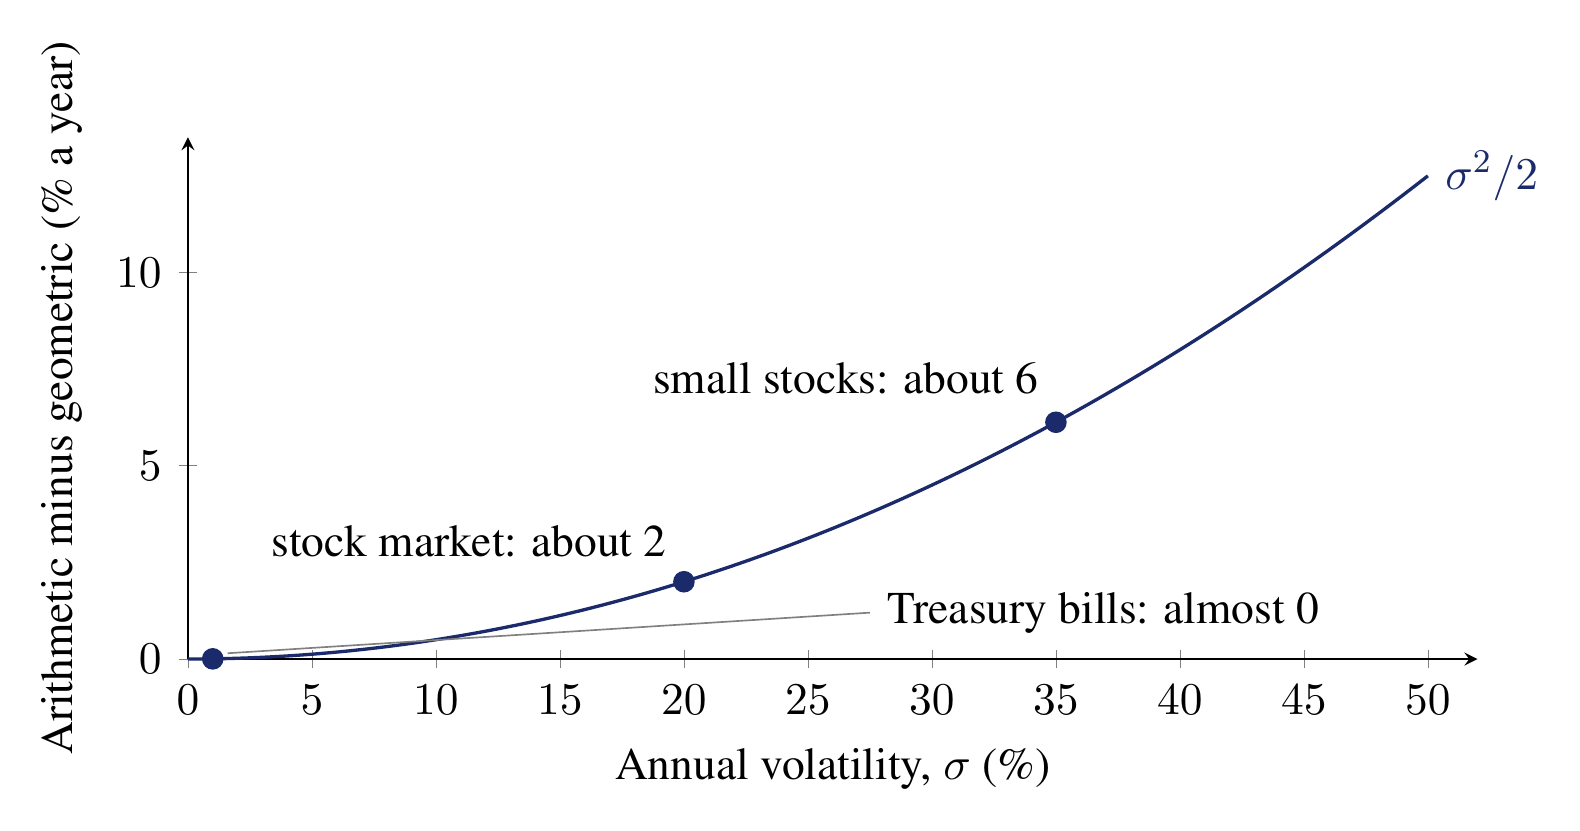
\includegraphics[width=0.85\linewidth]{images/fig02-1-volatility-drag.png}
\caption{Volatility drag: the gap between the arithmetic and geometric average returns, from Equation~\eqref{eq:02-drag}. The gap is negligible for Treasury bills, about 2 percentage points a year for the stock market and about 6 for small stocks, and it rises with the square of volatility.}
\label{fig:02-drag}
\end{figure}

Use the arithmetic average when you need the expected return for a single
period, as in the Sharpe ratio or a forecast. Use the geometric average when you
report how much an investment grew. If you quote the arithmetic average as the
growth rate, you will overstate the investor's experience, and the overstatement
is largest for exactly the volatile strategies that tend to look most
attractive. When a source reports an average return, check which kind it is.
Lab 2 measures the gap on real portfolios.

\section{Research datasets and their free alternatives}
\label{sec:02-datasets}

A result can be no more reliable than the data behind it. Each dataset covers
different companies, periods and events, and each handles corrections,
dividends and failed companies in its own way. If you do not know what your
dataset contains and what it leaves out, you cannot tell whether a result
reflects the market or the database.

Most published research on U.S. stocks rests on the two commercial databases introduced in Section~\ref{sec:02-foundations}, CRSP and Compustat. Two of their features matter most for this chapter, because free sources usually lack them: delisting returns and point-in-time data.


\begin{itemize}
  \item \textbf{CRSP} includes companies that later disappeared, along with the return in the month they delisted.
  \item \textbf{Compustat}'s point-in-time version records what was known on each date, rather than the figures as later revised.
\end{itemize}

Many universities subscribe; many readers will not have access. This book's labs use free sources that are built from, or comparable to, these databases:

\begin{center}
\small
\begin{tabularx}{0.9\linewidth}{@{}>{\raggedright\arraybackslash}p{0.22\linewidth}>{\raggedright\arraybackslash}X>{\raggedright\arraybackslash}p{0.26\linewidth}@{}}
\toprule
Free source & What it offers & Main limitation \\
\midrule
Kenneth R. French Data Library & Factor returns and portfolios sorted on size, value, momentum and more, built from CRSP and Compustat, since 1926 & Portfolio-level only; no individual stocks \\
FRED (Federal Reserve Bank of St.\ Louis) & Interest rates and economic series; its ALFRED archive keeps past vintages of revised data & Economic series, not stock-level data \\
Open Source Asset Pricing (Chen and Zimmermann) & Portfolio returns for over 200 published predictors & Full firm-level signals require WRDS \\
Jensen--Kelly--Pedersen global factors & 153 factors across 93 countries & Factor-level only \\
Yahoo Finance and similar & Daily prices for current stocks, ETFs and indexes & Mostly survivors only; adjustments not always documented; unofficial access methods can break \\
\bottomrule
\end{tabularx}
\end{center}

A \textbf{predictor} (or signal) is a variable, such as a valuation ratio or past return, that a study uses to forecast returns. The last row of the table deserves emphasis. Free stock-price sites are convenient, but they mostly cover companies that exist today. A backtest that pulls today's stocks from such a source and runs them through the past has survivorship bias built in, the problem Section~\ref{sec:02-survivorship} describes.

\section{Survivorship bias: the missing failures}
\label{sec:02-survivorship}

Companies that fail, merge or are delisted disappear from many datasets, and
their final losses disappear with them. A backtest run only on companies that
still exist never suffers those losses, so it overstates returns, often by
several percentage points a year. This is one of the most common errors in
practice, because most free price sources list only today's stocks.

\textbf{Survivorship bias} arises when a sample includes only the companies, funds or strategies that are still around at the end of the period. The ones that failed, were acquired or were shut down disappear from the data, and with them their losses. It is like judging how safe a sport is by interviewing only the players who are still playing.

The bias works through three channels:

\begin{enumerate}
  \item \textbf{Survivors-only samples.} Testing a strategy on today's index members, or on funds that exist today, removes every company or fund that failed along the way. The survivors are, by definition, the ones that did well enough to last.
  \item \textbf{Missing delisting returns.} When a stock leaves the exchange because it is failing, its final return is often large and negative, and often missing from the database. Shumway (1997) showed that CRSP frequently lacked returns for performance-related delistings and estimated that the missing returns averaged about $-30$\% for NYSE and AMEX stocks; Shumway and Warther (1999) found larger losses for Nasdaq stocks. A backtest that silently drops these months overstates returns, most of all for small and distressed stocks.
  \item \textbf{Backfill.} Databases sometimes add a company or fund with its history filled in after it has already succeeded. This \textbf{backfill} brings in past returns only for those that did well. Kothari, Shanken and Sloan (1995) argued that this kind of selection in Compustat inflated the measured returns of high book-to-market stocks, companies whose accounting value is large relative to their market value.
\end{enumerate}

For mutual funds the bias is well documented. Elton, Gruber and Blake (1996) estimated that studying only surviving funds overstated average performance by roughly 0.9 percentage points a year, a large number compared with the alphas researchers try to detect. Brown, Goetzmann, Ibbotson and Ross (1992) showed that survivorship can even make fund performance appear to persist from one period to the next when it does not.

\textbf{Why survivorship can create a strategy out of nothing.} The bias is not just a uniform upward shift. It favors the stocks most likely to fail: small, volatile, \textbf{distressed} companies, those at real risk of bankruptcy. Among those, the survivors are the ones that happened to rise. A survivors-only backtest of a strategy that buys volatile or distressed stocks can therefore show a large premium that is entirely produced by the sample. Lab 2 demonstrates this with a simulation in which the true premium is known to be zero.

\textbf{The fix} is a dataset that includes dead companies and their delisting returns, such as CRSP, and portfolio rules that use only firms listed at each date. When delisting returns are missing, researchers substitute estimates (for example $-30$\%) following Shumway.

\section{Look-ahead bias: using only what was known}
\label{sec:02-lookahead}

A backtest is honest only if every decision uses information that was
available at the time. Accounting figures are published weeks or months after
the period they describe, and economic data are often revised later. Using the
final numbers as if they were known in advance gives a strategy an advantage no
investor had, and the result can look excellent for no real reason.

\textbf{Look-ahead bias} arises when a backtest uses information that was not available at the time the decision would have been made. It is easy to introduce and hard to see, because the code runs without error and the results simply look better than they should. Figure~\ref{fig:02-timeline} shows the most common case: accounting data used before it was published.

\begin{figure}[htbp]
\centering
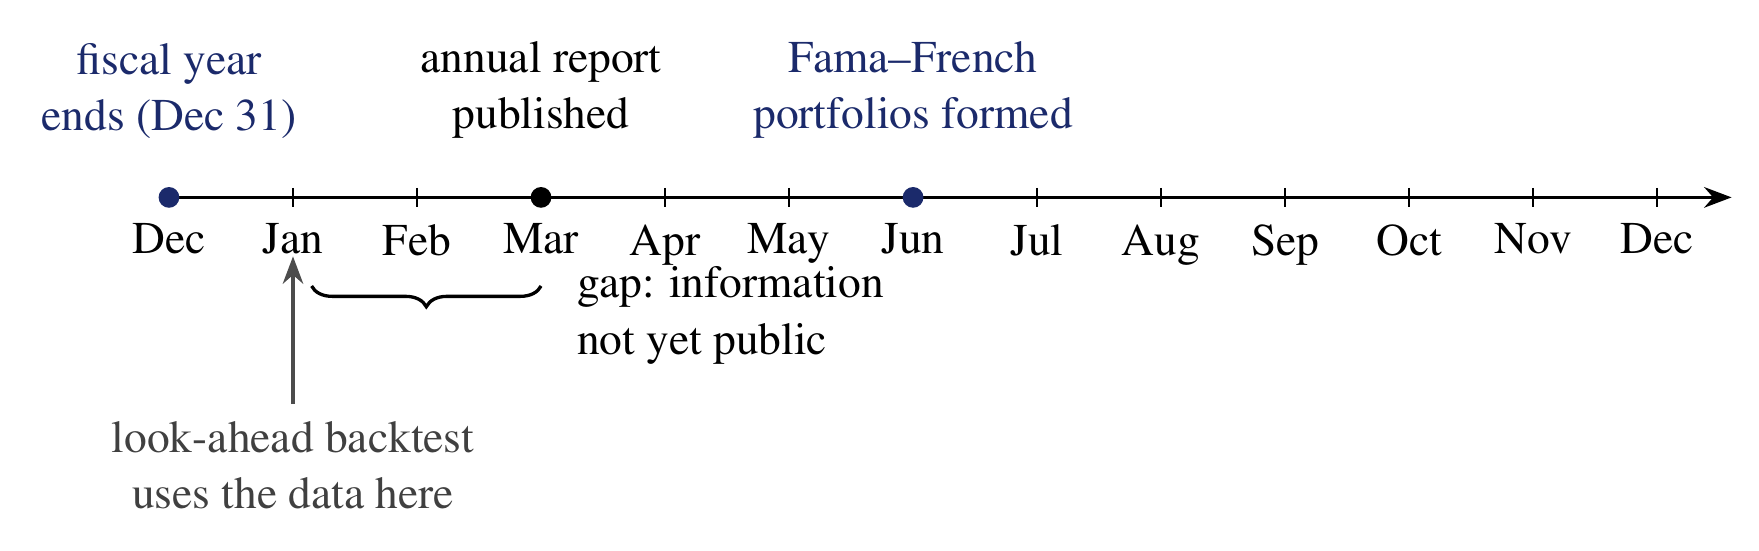
\includegraphics[width=0.9\linewidth]{images/fig02-2-accounting-timeline.png}
\caption{When accounting data becomes usable. A company's fiscal year ends in December, but its annual report appears only months later. A backtest that trades on the figures in January uses information no investor had. Fama and French wait until the following June to be safe.}
\label{fig:02-timeline}
\end{figure}

Common sources, and the standard defense against each:

\begin{center}
\small
\begin{tabularx}{0.9\linewidth}{@{}>{\raggedright\arraybackslash}p{0.16\linewidth}>{\raggedright\arraybackslash}X>{\raggedright\arraybackslash}p{0.32\linewidth}@{}}
\toprule
Source & What goes wrong & Standard defense \\
\midrule
Same-period execution & A signal computed from today's closing price is used to trade at that same close & Trade on the next period's return: lag every signal by at least one period \\
Accounting publication lags & Annual results for a December fiscal year are used in January, though they are published weeks or months later & Lag accounting data; Fama and French (1993) use fiscal-year data only from the following June \\
Revised economic data & GDP or employment figures are used as revised years later, not as first reported & Use real-time vintages, such as FRED's ALFRED archive \\
Index membership & Today's index members are used for the past & Use historical membership lists \\
Full-sample choices & Parameters, thresholds or variable definitions are chosen using the whole sample, then ``tested'' on it & Choose using only data available at each date (walk-forward; Chapter 5) \\
Full-sample scaling & Signals are standardized with means and volatilities computed over the whole sample & Use expanding or rolling estimates \\
\bottomrule
\end{tabularx}
\end{center}

Three terms in the table need a word of explanation. To \textbf{lag} a signal is to use it only from a later period, so that it was known before the trade. A \textbf{walk-forward} test chooses its settings at each date using only data before that date, as an investor in real time would have to. An \textbf{expanding} estimate uses all data up to each date; a \textbf{rolling} one uses a fixed window, such as the past five years.

The last two rows are the subtlest. No future price is used directly, yet the analyst's choices encode knowledge of how the whole period turned out. A trading rule whose window length was picked because it worked best over 1926--2025 carries information from 2025 back into 1926.

\textbf{Point-in-time data} is the general remedy: for each date, use only the values that were knowable then. Lab 2 measures two forms of look-ahead on real data: trading on the same day's close, and choosing a rule's parameter with hindsight.

\section{Micro-caps: results no investor could capture}
\label{sec:02-microcaps}

The smallest companies are costly or impossible to trade in size, yet in an
equal-weighted portfolio they carry the same weight as the largest. A result can
therefore be driven almost entirely by stocks no investor could realistically
buy. Checking how a portfolio is weighted, and whether the result survives
without the smallest stocks, is one of the quickest tests of whether a finding
is usable.

The U.S. stock market is extremely unequal. A few hundred large companies make up most of its value, while thousands of tiny companies make up most of its names. Fama and French (2008) classified stocks below the 20th percentile of NYSE market capitalization as \textbf{micro-caps}, meaning companies smaller than four-fifths of the stocks listed on the New York Stock Exchange. They found that micro-caps were about 60\% of all listed stocks but only about 3\% of total market value (Figure~\ref{fig:02-microcaps}).

\begin{figure}[htbp]
\centering
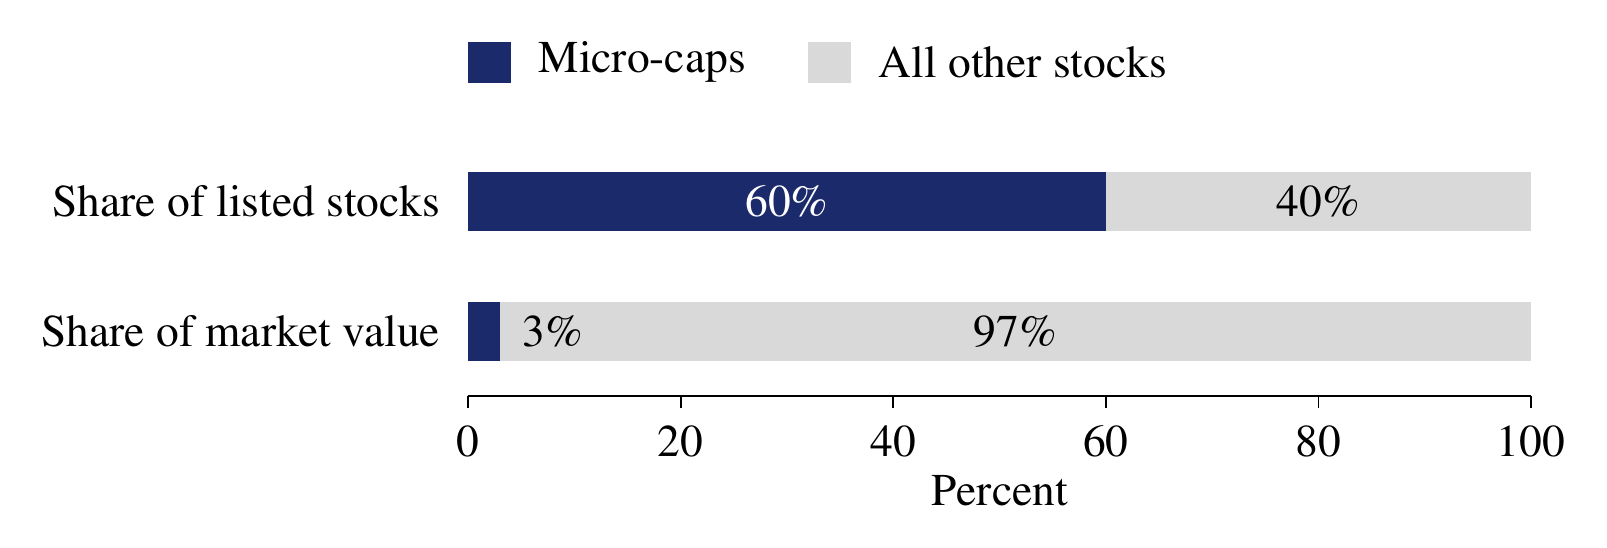
\includegraphics[width=0.8\linewidth]{images/fig02-3-microcaps.png}
\caption{Micro-caps are most of the stocks but almost none of the money. Source: Fama and French (2008).}
\label{fig:02-microcaps}
\end{figure}

This matters because of how portfolios are weighted (Section~\ref{sec:02-foundations}):

\begin{itemize}
  \item \textbf{Equal-weighted} portfolios give every stock the same weight, so micro-caps dominate them by number.
  \item \textbf{Value-weighted} portfolios weight stocks by market capitalization, so they reflect where investors' money actually is.
\end{itemize}

Micro-caps are expensive and difficult to trade. Their \textbf{bid--ask spreads}, the gap between the price at which you can buy and the price at which you can sell, are wide. They have little \textbf{liquidity}: buying or selling even a modest amount moves the price. And they are costly to \textbf{sell short}, that is, to borrow and sell in the hope of buying back more cheaply. They also have the most extreme returns and the most data problems, including the missing delisting returns of Section~\ref{sec:02-survivorship}. A pattern that appears in equal-weighted portfolios but not value-weighted ones may exist only where no large investor can exploit it.

The replication debate in Chapter 10 turns partly on this point. An \textbf{anomaly} is a pattern in returns that standard risk models, such as the CAPM, cannot explain. Hou, Xue and Zhang (2020) found that many anomalies fail when micro-caps are given little weight; their critics argue that this mainly shows anomalies are concentrated among small stocks. Either way, the lesson for this chapter is simple: \textbf{always ask how a portfolio is weighted and whether the result survives without micro-caps.}

\begin{callout}
\textbf{What Failed: the size effect.} Banz (1981) found that small companies had earned higher risk-adjusted returns than large ones, and ``small beats big'' became one of the best-known findings in finance. Later research found the effect much weaker after its publication, heavily concentrated among the very smallest stocks, and in early studies concentrated in January. Size remains a common factor in models of risk, but as a stand-alone source of extra return it has been far less reliable than its early evidence suggested. Lab 2 tests how much of the size premium comes from micro-caps and from the years before 1981.
\end{callout}

\section{Data snooping: when a whole field searches one dataset}
\label{sec:02-snooping}

Chapter 1 described selection within one researcher's search. There is a wider version: an entire field searching the same data. Most U.S. stock research uses CRSP, much of it the same post-1963 period. Thousands of researchers have tested thousands of ideas on it, and the ideas that ``worked'' were published. Each paper may report a single, honest test, yet collectively the field has run an enormous number of trials on one history. A finding can therefore be a false discovery even when its author did nothing wrong, which is why a result must be confirmed on data that played no part in finding it.

Lo and MacKinlay (1990) called this \textbf{data-snooping bias}: when the choice of what to test is influenced by what earlier studies found in the same data, standard significance levels overstate the evidence. The bias cannot be fixed by any single researcher, because no one knows how many ideas were tried and abandoned across the field.

Three defenses work, and later chapters use all of them:

\begin{enumerate}
  \item \textbf{New data.} Test the claim in periods or markets that played no part in its discovery: before the original sample, after publication, or in other countries (Chapters 8--10).
  \item \textbf{Higher hurdles.} Require stronger evidence for claims tested on heavily used data, such as a t-statistic above 3 (Harvey, Liu and Zhu 2016; Chapter 4).
  \item \textbf{Economic reasoning stated in advance.} A claim backed by a mechanism specified before the test is less likely to be a statistical accident than one explained after the fact.
\end{enumerate}

\section{Lab 2: Four ways data can mislead}
\label{sec:02-lab}

\begin{callout}
\textbf{Lab 2 at a glance.} \emph{Claim on trial:} free, public data can support a reliable backtest. \emph{Data:} monthly and daily U.S. market returns and size-sorted portfolios since 1926, from the Kenneth R. French Data Library (downloaded automatically), plus a simulated stock market. \emph{Tools:} Python with pandas, NumPy and matplotlib, plus the fintest module. \emph{Time:} about 90 minutes, including the guided notebook. \emph{Code:} repository folder \texttt{ch02-data-traps/}.
\end{callout}

The lab measures each problem from Sections~\ref{sec:02-returns} to~\ref{sec:02-microcaps} in turn. Three parts use real data. Survivorship uses a simulation, for a reason that is itself part of the lesson: free data sources do not include the companies that disappeared, which is exactly the data needed to measure the bias.

\subsection*{Part A: Arithmetic versus geometric averages}

\textbf{Predict first.} Write down which of four portfolios you expect to show
the largest gap between its arithmetic and geometric average returns, and
roughly how large.

The lab computes both averages for Treasury bills, the stock market, and the
largest and smallest 10\% of stocks, annualizing each in the same way so the
comparison is like for like. It then compares each measured gap with the
volatility-drag approximation from Section~\ref{sec:02-returns}: the geometric
average is roughly the arithmetic average minus half the variance,
$G \approx A - \sigma^2/2$ (Figure 2.4). Expect almost no gap for Treasury
bills, about 2 percentage points a year for the market, and the largest gap,
several points a year, for the smallest stocks. If the measured and approximate
gaps differ, ask why: the approximation assumes returns are close to normal,
and small stocks are not.

\subsection*{Part B: Survivorship bias in a market where the truth is known}

\textbf{Predict first.} Before running this part, write down how much you
expect survivorship bias to add to the market's average return each year.

With real data we never know the true answer, so the lab builds a market where
we do. It simulates about 2,000 listed companies over 30 years, and every
company has the \textbf{same expected return}: no stock or strategy has a real
advantage. A company whose price falls below 20\% of its listing price is
delisted with a final return of $-30$\%, following Shumway (1997). Other
companies are acquired at a premium, and every company that leaves is replaced
by a new listing.

From this one simulated history, the lab builds three datasets:

\begin{center}
\small
\begin{tabularx}{0.9\linewidth}{@{}>{\raggedright\arraybackslash}p{0.26\linewidth}>{\raggedright\arraybackslash}X>{\raggedright\arraybackslash}p{0.28\linewidth}@{}}
\toprule
Dataset & What it contains & Real-world equivalent \\
\midrule
Full data & Every company, including its delisting return & CRSP, used correctly \\
Missing delisting returns & Every company, but without the final delisting month & A database with gaps in delisting returns \\
Survivors only & Only companies still listed at the end & Today's stocks downloaded from a free price site \\
\bottomrule
\end{tabularx}
\end{center}

On each dataset, the lab measures two things: the equal-weighted market return,
and the return of a strategy that each month buys the most volatile fifth of
stocks and sells the least volatile fifth, sorted on past volatility only
(Figure 2.5). The full data give the true answer. Any difference in the other
two datasets comes entirely from how they were built.

With the lab's default settings (2,000 listed companies, 30 years, seed 2026),
5,856 companies are listed over the period, 1,693 are delisted for poor
performance, and 2,000 survive to the end. The results:

\begin{center}
\small
\begin{tabularx}{0.9\linewidth}{@{}>{\raggedright\arraybackslash}X>{\raggedright\arraybackslash}p{0.22\linewidth}>{\raggedright\arraybackslash}p{0.22\linewidth}r@{}}
\toprule
Dataset & Equal-weighted compound return & Volatile minus calm, per year & t-statistic \\
\midrule
Full data & 9.3\% & $-1.2$\% & $-2.2$ \\
Missing delisting returns & 10.7\% & $+2.0$\% & 3.5 \\
Survivors only & 14.0\% & $+12.0$\% & 14.7 \\
\bottomrule
\end{tabularx}
\end{center}

Read the table from top to bottom. In the full data, the volatile-minus-calm
strategy loses about 1\% a year, because volatile companies are delisted more
often. Leaving out only the delisting returns flips the sign: the strategy now
appears to earn 2\% a year. Keeping only the survivors adds almost five
percentage points a year to the market's return and creates a ``volatility
premium'' of 12\% a year, with a t-statistic far beyond any hurdle in this book.
None of it is real. Compare these numbers with your prediction.

\subsection*{Part C: Look-ahead bias}

\textbf{Predict first.} Write down whether you expect a one-day timing error to
change a strategy's Sharpe ratio a little or a lot.

\textbf{C1. Trading on the same day's close.} Test a classic timing rule: hold
stocks when the market closes above its 200-day \textbf{moving average}, the
average closing price over the past 200 trading days, and hold Treasury bills
otherwise. Run it two ways. The correct version decides at yesterday's close and
earns today's return. The look-ahead version decides at today's close but is
still credited with today's return. The difference is a single day, the kind of
error that can hide in one misplaced line of code. Compare the two versions'
returns and Sharpe ratios (Figure 2.6).

\textbf{C2. Choosing the window with hindsight.} Now test moving-average windows
from 20 to 300 days, and choose one in two ways. The hindsight version picks the
window with the best Sharpe ratio over the whole evaluation period. The
walk-forward version picks, each January, the window that had worked best up to
that point, using only past data (Figure 2.7). The gap between the two measures
how much a result is inflated by choosing a rule's settings after seeing the
results.

\subsection*{Part D: Micro-caps, weighting and the size premium}

\textbf{Predict first.} Write down whether you expect the size premium to be
larger in value-weighted or equal-weighted portfolios, and whether it survives
after 1981.

Using size-sorted portfolios, the lab measures the \textbf{size premium}, the
return of the smallest tenth of stocks minus the largest tenth, four ways:
value-weighted and equal-weighted, and with and without the smallest tenth of
stocks. It then splits the sample before and after Banz's 1981 publication
(Figure 2.8). Together these test the What Failed box in
Section~\ref{sec:02-microcaps} directly: if the premium lives mainly in tiny,
hard-to-trade stocks or disappears after it was published, the claim weakens.

\emph{[Draft note: figures and numbers for Parts A, C and D are generated from the Kenneth R. French data at the time of publication; the book prints those results. The Part B simulation is fixed by design and its results can be printed as they stand.]}

\subsection*{Your verdict}

Readers write one sentence per problem, saying how much it changed the result and in which direction, and then judge the claim. The expected verdict is \textbf{survives, with conditions}. Free data can support a reliable backtest when you:

\begin{enumerate}
  \item use total returns and compare them with a total-return benchmark, quoting the geometric average for growth (Part A);
  \item use data that include failed companies, such as the French library's portfolios, which are built from CRSP, rather than a list of today's stocks (Part B);
  \item lag every signal and every accounting figure, and choose a rule's settings with walk-forward tests (Part C);
  \item check that the result survives value weighting and the removal of micro-caps (Part D).
\end{enumerate}

A backtest that skips these steps can look excellent and mean nothing; one that follows them can be trusted as far as its statistics allow. The checklist in the next section turns these conditions into questions you can ask of any backtest, including your own.

\section{What investors can use: a data checklist}
\label{sec:02-checklist}

Before trusting any backtest, your own or someone else's, run through these questions. Each maps to a section of this chapter, and most can be answered in a few minutes.

\begin{itemize}
  \item[$\square$] \textbf{Returns (Section~\ref{sec:02-returns}):} Are returns total returns, including dividends? Are they compared with a total-return benchmark? Is the reported average arithmetic or geometric?
  \item[$\square$] \textbf{Excess returns (Section~\ref{sec:02-returns}):} Is performance measured above the risk-free rate?
  \item[$\square$] \textbf{Survivorship (Section~\ref{sec:02-survivorship}):} Does the dataset include companies or funds that no longer exist? Are delisting returns included?
  \item[$\square$] \textbf{Look-ahead (Section~\ref{sec:02-lookahead}):} Is every signal lagged so it uses only information available before the trade? Are accounting data lagged to their publication dates?
  \item[$\square$] \textbf{Hindsight choices (Section~\ref{sec:02-lookahead}):} Were parameters, thresholds or universes chosen using the whole sample?
  \item[$\square$] \textbf{Weighting (Section~\ref{sec:02-microcaps}):} Is the portfolio value- or equal-weighted? Does the result survive without micro-caps?
  \item[$\square$] \textbf{Shared data (Section~\ref{sec:02-snooping}):} Has the result been tested on data that played no part in its discovery: other periods, other markets, or after publication?
\end{itemize}

\textbf{Questions to ask a fund manager or strategy vendor}

\begin{itemize}
  \item Which database was the backtest built on, and does it include delisted stocks and delisting returns?
  \item How were signals lagged, and when would each piece of data actually have been available?
  \item Is the strategy value- or equal-weighted, and what share of its return comes from the smallest stocks?
  \item Is the reported return arithmetic or compound, and before or after costs?
\end{itemize}

\section*{Exercises}
\addcontentsline{toc}{section}{Exercises}

\subsection*{Conceptual (all readers)}

\begin{enumerate}
  \item A strategy reports an average annual return of 18\% with volatility of 40\%. Estimate its geometric average. Which number should an investor care about, and why?
  \item Explain why a portfolio's simple return is a weighted average of its holdings' simple returns, while a multi-period return is a sum of log returns.
  \item A researcher backtests a strategy on the stocks in today's S\&P 500 index from 2005 to today. List two biases in this design and the direction of each.
  \item A study uses annual accounting data for fiscal years ending in December and forms portfolios in January of the next year. What is the problem, and how do Fama and French avoid it?
  \item Explain why survivorship bias can create a premium for volatile stocks, not just raise all returns equally.
  \item A paper reports a strong anomaly in equal-weighted portfolios that disappears in value-weighted ones. What does this suggest about who could profit from it?
\end{enumerate}

\subsection*{Lab extensions (technical readers)}

\begin{enumerate}
  \setcounter{enumi}{6}
  \item Re-run Part B with a delisting return of $-55$\%, closer to estimates for Nasdaq stocks. How do the three datasets change?
  \item In Part C, try windows of 50 and 300 days. Is the look-ahead gain larger for fast or slow rules? Explain.
  \item In Part C, charge a trading cost of 0.1\% each time the rule switches. Does the correctly traded rule still beat buy-and-hold on a risk-adjusted basis?
  \item In Part D, move the publication split to 1990 and 2000. When does the size premium appear to fade?
  \item \textbf{Challenge:} using a free price source, backtest an equal-weighted portfolio of today's S\&P 500 members over the past 20 years and compare it with the equal-weighted S\&P 500 index. Which problem from this chapter explains the difference?
\end{enumerate}

\section*{References}
\addcontentsline{toc}{section}{References}

\begin{itemize}
  \item Banz, R. W. (1981). The Relationship Between Return and Market Value of Common Stocks. \emph{Journal of Financial Economics} 9(1): 3--18.
  \item Brown, S. J., Goetzmann, W., Ibbotson, R. G. and Ross, S. A. (1992). Survivorship Bias in Performance Studies. \emph{Review of Financial Studies} 5(4): 553--580.
  \item Elton, E. J., Gruber, M. J. and Blake, C. R. (1996). Survivorship Bias and Mutual Fund Performance. \emph{Review of Financial Studies} 9(4): 1097--1120.
  \item Fama, E. F. and French, K. R. (1993). Common Risk Factors in the Returns on Stocks and Bonds. \emph{Journal of Financial Economics} 33(1): 3--56.
  \item Fama, E. F. and French, K. R. (2008). Dissecting Anomalies. \emph{Journal of Finance} 63(4): 1653--1678.
  \item Harvey, C. R., Liu, Y. and Zhu, H. (2016). \ldots and the Cross-Section of Expected Returns. \emph{Review of Financial Studies} 29(1): 5--68.
  \item Hou, K., Xue, C. and Zhang, L. (2020). Replicating Anomalies. \emph{Review of Financial Studies} 33(5): 2019--2133.
  \item Kothari, S. P., Shanken, J. and Sloan, R. G. (1995). Another Look at the Cross-Section of Expected Stock Returns. \emph{Journal of Finance} 50(1): 185--224.
  \item Lo, A. W. and MacKinlay, A. C. (1990). Data-Snooping Biases in Tests of Financial Asset Pricing Models. \emph{Review of Financial Studies} 3(3): 431--467.
  \item Shumway, T. (1997). The Delisting Bias in CRSP Data. \emph{Journal of Finance} 52(1): 327--340.
  \item Shumway, T. and Warther, V. A. (1999). The Delisting Bias in CRSP's Nasdaq Data and Its Implications for the Size Effect. \emph{Journal of Finance} 54(6): 2361--2379.
\end{itemize}

\textbf{Data:} Kenneth R. French Data Library: Fama/French 3 Factors (monthly and daily); Portfolios Formed on Size. \url{https://mba.tuck.dartmouth.edu/pages/faculty/ken.french/data_library.html}

% Chapter 3 -- Statistics for Noisy Returns
% Requires: amsmath, amssymb, booktabs, array, tabularx, graphicx, tcolorbox (breakable, skins), hyperref or url.
% Defines the callout box only if the preamble has not.
\providecolor{fenavy}{HTML}{1B2A6B}
\providecolor{feshade}{HTML}{F3F5FA}
\makeatletter
\@ifundefined{callout}{%
  \newtcolorbox{callout}{breakable, enhanced,
    colback=white, colframe=gray!70, boxrule=0.5pt, arc=1mm,
    borderline west={2.5pt}{0pt}{gray!70},
    left=8pt, right=8pt, top=4pt, bottom=4pt}%
}{}
\makeatother

\chapter{Statistics for Noisy Returns}
\label{ch:03}

Part II of the book turns the lessons of Part I into tools. It begins with the most basic tool of all: the t-statistic.

Almost every claim in quantitative finance ends in a number like ``$t = 2.4$.'' That number comes from formulas taught in introductory statistics, which assume that observations are independent, that their spread is constant, and that their distribution is roughly normal. Financial returns satisfy none of these assumptions exactly. Their tails are fat, their volatility comes in clusters, and some of the most popular research designs build in strong dependence between observations. The good news is that each departure has a well-tested remedy, and choosing the right one is a skill you can learn in a single chapter.

The claim on trial in this chapter is the one every researcher relies on: \textbf{with the right standard errors, regression statistics are reliable for financial returns.} The lab tests it in two settings: one where the usual formulas already work well, and one where the choice of standard error decides whether a ``significant'' result is real.

By the end of the chapter you will be able to:

\begin{itemize}
  \item summarize a return distribution by its mean, variance, skewness, kurtosis and autocorrelation;
  \item run and interpret a linear regression, including its slope, intercept and $R^2$, and explain what heteroskedasticity and serial correlation do to its standard errors;
  \item explain the CAPM and the Fama--French three-factor model, and interpret beta and alpha;
  \item describe the stylized facts of financial returns: fat tails, volatility clustering, weak autocorrelation and asymmetry;
  \item choose standard errors that remain valid when those features are present: White, Newey--West and clustered errors;
  \item explain why overlapping long-horizon regressions mislead, and how to correct them;
  \item test a factor model with alphas, the GRS test and Fama--MacBeth regressions;
  \item use the bootstrap to measure uncertainty without relying on normality;
  \item separate statistical significance from economic significance.
\end{itemize}

In the lab you will measure these features on nearly a century of real data, compute the alphas of 25 classic portfolios four different ways, and run a controlled experiment that shows how often overlapping regressions find predictability that is not there.

\section{Foundations: distributions, regression and factor models}
\label{sec:03-foundations}

\textbf{Describing a distribution.} Four numbers, called \textbf{moments}, summarize a return distribution.

\begin{itemize}
  \item The \textbf{mean} is its center: the average return.
  \item The \textbf{variance}, or its square root the standard deviation, measures spread: how far returns typically fall from the mean.
  \item \textbf{Skewness} measures asymmetry. It is negative when large losses are more likely than large gains of the same size, as for most stock indexes.
  \item \textbf{Kurtosis} measures how heavy the tails are. A normal distribution has kurtosis 3; values above 3 indicate \textbf{fat tails}, meaning extreme returns occur more often than a normal distribution predicts.
\end{itemize}

Figure~\ref{fig:03-moments} shows what each of the four moments changes, by comparing the normal distribution with one that differs in that moment alone.

\begin{figure}[htbp]
\centering
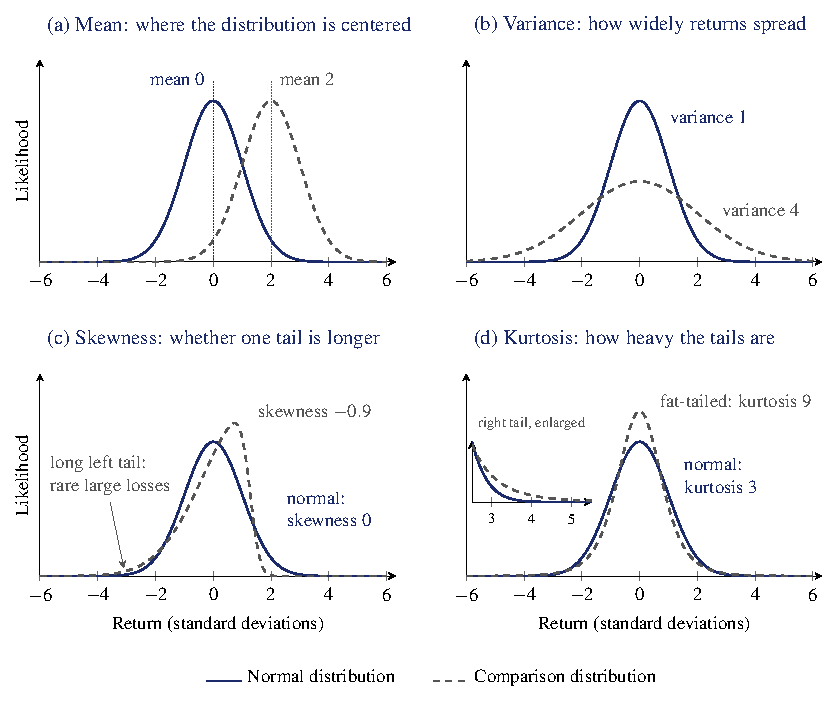
\includegraphics[width=0.95\linewidth]{images/fig03-0-moments.pdf}
\caption{The four moments of a distribution. Each panel compares the standard normal distribution (solid) with one that differs in a single respect. (a)~The mean sets the center. (b)~The variance sets the spread. (c)~Negative skewness lengthens the left tail, so large losses are more likely than large gains of the same size. (d)~Higher kurtosis puts more weight in the tails: the normal distribution has kurtosis 3, the fat-tailed one shown has kurtosis 9. Panels (c) and (d) keep the mean and variance of the normal distribution.}
\label{fig:03-moments}
\end{figure}

A fifth measure describes behavior over time. \textbf{Autocorrelation} is the correlation of a series with its own past values: the first-order autocorrelation compares each month with the month before. A return series with zero autocorrelation cannot be predicted from its own history.

\textbf{Linear regression.} A regression describes how one variable, $y$, moves with another, $x$. Ordinary least squares (OLS) fits
\begin{equation}
  y_t = \alpha + \beta x_t + \varepsilon_t
  \label{eq:03-ols}
\end{equation}
by choosing the intercept $\alpha$ and slope $\beta$ that make the \textbf{residuals} $\varepsilon_t$, the gaps between the actual values and the fitted line, as small as possible in the sense of their sum of squares. The slope $\beta$ measures how much $y$ moves when $x$ moves by one unit. The \textbf{R-squared}, $R^2$, is the share of the variance of $y$ that the regression explains, from 0 (none) to 1 (all).

Each estimate comes with a standard error, and the usual formula for it assumes that the residuals are independent of one another and have the same variance throughout. Two departures from these assumptions are common in finance:

\begin{itemize}
  \item \textbf{Heteroskedasticity}: the variance of the residuals changes over time or across observations, for example rising in a crisis.
  \item \textbf{Serial correlation}: residuals are correlated with their own past values, so one large error tends to be followed by another.
\end{itemize}

When either is present, the coefficient estimates usually remain reasonable, but the usual standard errors are wrong, and the corrections developed in this chapter are needed.

\textbf{The capital asset pricing model.} The CAPM of Sharpe (1964), Lintner (1965) and Mossin (1966) says that an asset's expected excess return is proportional to its \textbf{beta}, its sensitivity to the market:
\begin{equation}
  E[R_i] - r_f = \beta_i \left(E[R_m] - r_f\right), \qquad \beta_i = \frac{\operatorname{Cov}(R_i, R_m)}{\operatorname{Var}(R_m)}
  \label{eq:03-capm}
\end{equation}
Here $\operatorname{Cov}$ is the covariance, which measures how two returns move together, and $\operatorname{Var}$ the variance. A stock with a beta of 1.5 tends to rise 1.5\% when the market rises 1\%. Only market risk is rewarded, because other risk can be removed by holding many stocks, which is called \textbf{diversification}. Empirically, the model is tested with a time-series regression of an asset's excess return on the market's excess return, as in Section~\ref{sec:01-foundations}. The intercept, \textbf{alpha}, is the average return the CAPM fails to explain; the model predicts that alpha is zero for every asset. Figure~\ref{fig:03-alpha} shows the two numbers on a scatter plot.

\begin{figure}[htbp]
\centering
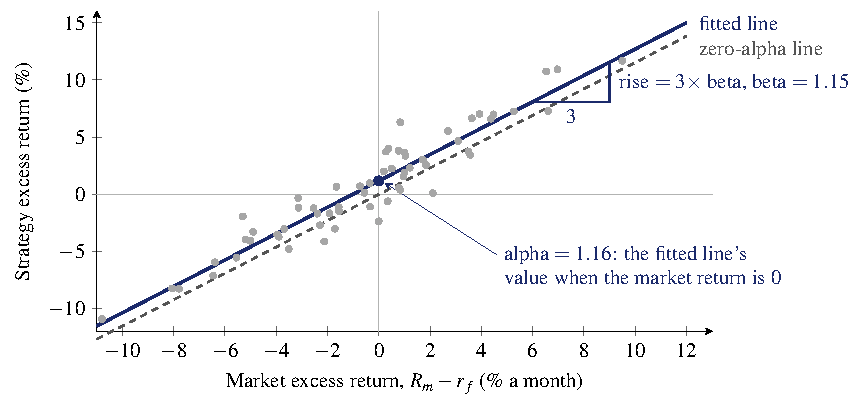
\includegraphics[width=0.85\linewidth]{images/fig03-1-regression-alpha.pdf}
\caption{Beta and alpha in a regression of a strategy's monthly excess returns on the market's. Beta is the slope of the fitted line; alpha is its height where the market's excess return is zero, the gap between the fitted line and a line with the same slope through the origin. Simulated data, with an alpha larger than any real strategy's so that it is visible.}
\label{fig:03-alpha}
\end{figure}

\textbf{Multifactor models.} The CAPM fits the data poorly: small stocks and value stocks have earned more than their betas imply (Chapter 8). \textbf{Factor models} add further sources of risk, called factors. The Fama--French three-factor model adds two:

\begin{itemize}
  \item SMB (small minus big): the return of small stocks over large ones;
  \item HML (high minus low): the return of value stocks, with high book-to-market ratios, over growth stocks, with low ones.
\end{itemize}

The model is
\begin{equation}
  R_i - r_f = \alpha_i + b_i(R_m - r_f) + s_i\,\mathrm{SMB} + h_i\,\mathrm{HML} + \varepsilon_i
  \label{eq:03-ff3}
\end{equation}
where $b_i$, $s_i$ and $h_i$ measure the asset's exposure to each factor. The factors are themselves \textbf{long--short} portfolio returns: each buys one group of stocks and sells the other short, so it costs roughly nothing to set up. A strategy's alpha relative to a factor model measures what it earns beyond its exposures to those factors.

\textbf{Testing many alphas at once.} If a model is correct, the alphas of all assets should be jointly zero. The GRS test (Gibbons, Ross and Shanken 1989) tests this for a set of portfolios. The \textbf{Fama--MacBeth} procedure (Fama and MacBeth 1973) asks a related question: is a characteristic or beta rewarded across assets? Each month it regresses returns across assets on their betas, then averages the monthly slopes over time. Sections~\ref{sec:03-grs} and~\ref{sec:03-fmb} develop both.

\textbf{Worked example.} A fund's monthly excess returns are regressed on the market's. The estimated beta is 1.1 and alpha is 0.2\% a month with a standard error of 0.15\%. The alpha's t-statistic is $0.2/0.15 = 1.33$: the fund may have skill, but the data cannot distinguish its alpha from zero.


\section{Stylized facts of financial returns}
\label{sec:03-facts}

The textbook standard error rests on three assumptions: observations are
independent, their variance is constant, and their distribution is roughly
normal. Real returns depart from all three in consistent ways. This section
describes the four departures that matter most, and shows which assumption each
one breaks.

Decades of research have documented these features across markets, assets and
periods. Cont (2001) collected them as ``stylized facts,'' patterns found so
consistently that any model of returns must reproduce them:

\begin{enumerate}
  \item \textbf{Fat tails.} Extreme returns happen far more often than a normal distribution predicts (Figure~\ref{fig:03-tails}). Mandelbrot (1963) and Fama (1965) documented this in the 1960s. On October 19, 1987, the U.S. market fell by more than 20\% in a day, a move a normal distribution fitted to daily data would treat as essentially impossible. For daily stock index returns, kurtosis is typically far higher than the normal distribution's 3.
  \item \textbf{Volatility clustering.} Large moves tend to follow large moves, of either sign, and calm periods follow calm periods. Returns themselves show little autocorrelation, but their absolute values and squares are strongly and persistently autocorrelated. Chapter 11 builds forecasting models on this feature.
  \item \textbf{Weak autocorrelation in returns.} Daily and monthly index returns show only small autocorrelations, consistent with Section~\ref{sec:01-efficient-markets}. Some portfolios, especially of small stocks, show more, partly because their prices are \textbf{stale}: some stocks do not trade every day, so their last recorded price lags the news.
  \item \textbf{Asymmetry.} Large falls are more common than large rises of the same size, and volatility tends to rise after falls. The rise in volatility after a fall is called the \textbf{leverage effect}, because a falling share price raises a company's debt relative to its equity.
\end{enumerate}

\begin{figure}[htbp]
\centering
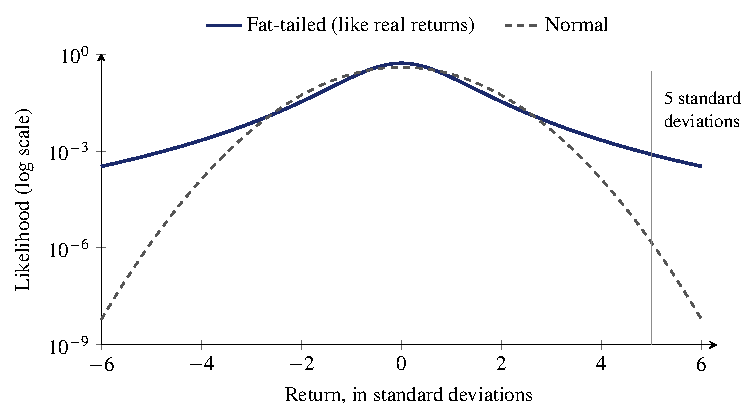
\includegraphics[width=0.85\linewidth]{images/fig03-2-fat-tails.pdf}
\caption{Fat tails. Both curves have the same mean and standard deviation. On a log scale the difference in the tails becomes visible: a daily move of five standard deviations in either direction occurs about once in 7,000 years under the normal distribution, but about once every two years under the fat-tailed distribution shown, a Student-$t$ distribution with four degrees of freedom, which is a common model for daily returns.}
\label{fig:03-tails}
\end{figure}

\textbf{Why this matters for statistics.} None of these features biases the
regression estimates themselves, which usually remain right on average. What
they damage is the stated precision of those estimates, and with it every
t-statistic and \textbf{p-value}, the probability of a result at least this
extreme if the true effect were zero (Chapter 4). Each feature breaks a
different assumption, and the rest of the chapter deals with each in turn:

\begin{center}
\small
\begin{tabularx}{0.95\linewidth}{@{}>{\raggedright\arraybackslash}p{0.26\linewidth}>{\raggedright\arraybackslash}X>{\raggedright\arraybackslash}p{0.33\linewidth}@{}}
\toprule
Feature & Assumption it breaks & Remedy \\
\midrule
Volatility clustering & Constant variance & White or Newey--West standard errors (Section~\ref{sec:03-se}) \\
Autocorrelation and stale prices & Independence & Newey--West standard errors (Section~\ref{sec:03-se}) \\
Overlapping research designs & Independence, severely & Newey--West with enough lags, or Hodrick (1992) (Section~\ref{sec:03-overlap}) \\
Fat tails & Normality, so small-sample p-values are off & The bootstrap (Section~\ref{sec:03-bootstrap}) \\
\bottomrule
\end{tabularx}
\end{center}

\section{Choosing the right standard error}
\label{sec:03-se}

The estimates from a regression are usually reliable even when returns violate
the textbook assumptions. Their standard errors are not. The right standard
error is the one that allows for the dependence your data actually have: errors
whose variance changes over time, errors that move together over time, or
errors that move together across firms.

Consider the regression that appears throughout this book, a time-series
regression of a portfolio's excess return on one or more factors:
\begin{equation}
  r_t = \alpha + \beta' f_t + \varepsilon_t
  \label{eq:03-ts}
\end{equation}
where $f_t$ is the list of factor returns in month $t$ and $\beta'$ the list of
the portfolio's exposures to them. The classical standard error assumes that
the errors $\varepsilon_t$ are independent and equally variable. Three
alternatives relax these assumptions one step at a time:

\begin{itemize}
  \item \textbf{White (1980)} allows the variance of the errors to change over
  time, as it does when volatility clusters.
  \item \textbf{Newey--West (1987)} also allows errors up to $L$ periods apart
  to be correlated. It is called a \textbf{HAC} estimator, for
  \emph{heteroskedasticity and autocorrelation consistent}.
  \item \textbf{Clustered} standard errors allow errors within a group, such as
  all firms in the same month, to be correlated (Petersen 2009).
\end{itemize}

\textbf{Which to use.} Match the standard error to the data:

\begin{center}
\small
\begin{tabularx}{0.95\linewidth}{@{}>{\raggedright\arraybackslash}p{0.34\linewidth}>{\raggedright\arraybackslash}p{0.28\linewidth}>{\raggedright\arraybackslash}X@{}}
\toprule
Your data & Use & Why \\
\midrule
Monthly returns, no overlap & White, or Newey--West with a few lags & Volatility changes, but errors are close to independent \\
Errors correlated over time (daily data, stale prices, persistent predictors) & Newey--West & Nearby errors move together \\
Overlapping $k$-period returns & Newey--West with at least $k-1$ lags, or Hodrick (1992) & The overlap builds in correlation $k-1$ periods long (Section~\ref{sec:03-overlap}) \\
Many firms over many periods & Clustered by firm and by time & Errors move together within a month and within a firm \\
\bottomrule
\end{tabularx}
\end{center}

When in doubt, report Newey--West. If the data have no dependence, it gives
almost the same answer as the classical formula, so little is lost; if they
do, it protects you from false confidence. Part B of the lab shows the first
case and Part C the second.

\textbf{Choosing the lag.} Newey--West needs one setting, the number of lags
$L$. A common rule of thumb is $L = \lfloor 4(T/100)^{2/9} \rfloor$, where
$\lfloor\cdot\rfloor$ means rounding down: 50 years of monthly data, $T = 600$,
gives $L = 5$. When the design creates dependence of a known length, such as
$k$-month overlapping returns, use at least $k - 1$ lags.

\textbf{How Newey--West works.} For readers who want the detail: every
standard error rests on an estimate of how much the regression's errors vary
and move together. Newey--West estimates it as
\begin{equation}
  \hat S = \sum_t x_t x_t' \hat\varepsilon_t^2 + \sum_{\ell=1}^{L} \left(1 - \frac{\ell}{L+1}\right) \sum_t \left(x_t \hat\varepsilon_t \hat\varepsilon_{t-\ell} x_{t-\ell}' + x_{t-\ell} \hat\varepsilon_{t-\ell} \hat\varepsilon_t x_t'\right)
  \label{eq:03-nw}
\end{equation}
where $x_t$ holds the regressors in period $t$. The first sum is White's
estimator, which lets each period have its own variance. The second adds the
correlations between errors up to $L$ periods apart, with weights that shrink
as the gap $\ell$ grows.

\section{Overlapping observations: less data than it seems}
\label{sec:03-overlap}

Long-horizon regressions can look far stronger than they are. When each
observation's return overlaps the next, a sample that seems to hold hundreds of
observations holds only a handful of independent ones, and the classical
t-statistic and $R^2$ overstate the evidence accordingly.

\textbf{The design.} A popular design in return-prediction research regresses
returns over a long horizon, such as the next five years, on a predictor
measured today, such as the dividend yield:
\begin{equation}
  r_{t+1} + r_{t+2} + \dots + r_{t+k} = a + b\,x_t + u_{t+k}
  \label{eq:03-longhorizon}
\end{equation}

\textbf{The problem: counting observations.} With monthly data and $k = 60$,
each observation's dependent variable shares 59 of its 60 months with the next
observation's (Figure~\ref{fig:03-overlap}). The regression appears to have
hundreds of observations but contains roughly $T/k$ independent ones. Fifty
years of monthly data, $T = 600$, give only $600/60 = 10$ independent five-year
returns.

\begin{figure}[htbp]
\centering
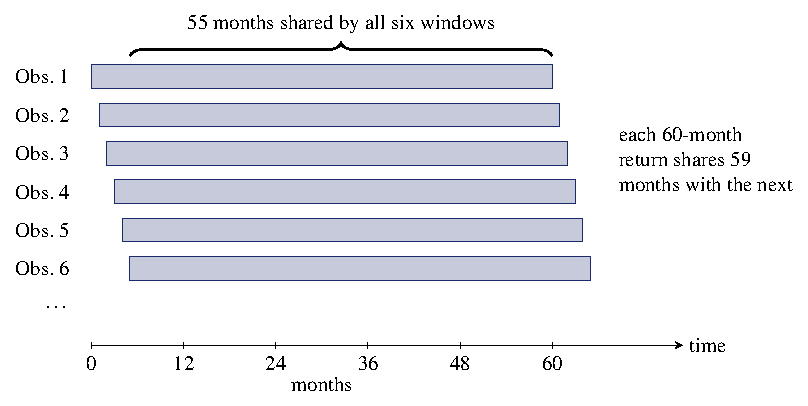
\includegraphics[width=0.85\linewidth]{images/fig03-3-overlap.pdf}
\caption{Overlapping observations. Each observation in a regression of five-year returns covers 60 months, and each starts one month after the last. Consecutive observations share 59 of their 60 months, so they carry almost the same information.}
\label{fig:03-overlap}
\end{figure}

\textbf{Two consequences.}

\begin{enumerate}
  \item \textbf{Standard errors that are far too small.} The errors $u$ are strongly autocorrelated by construction, up to lag $k - 1$. Classical standard errors ignore this and can be several times too small. Hansen and Hodrick (1980) and Newey--West correct for the overlap, but in samples of typical length they still reject a true null hypothesis too often. A test's \textbf{size} is the rate at which it does so; a well-behaved 5\% test has a size of 5\%. Hodrick (1992) proposed an alternative that avoids overlapping errors and has more reliable size.
  \item \textbf{Biased slopes from persistent predictors.} A variable is \textbf{persistent} when it moves slowly, so that this month's value is close to last month's. The dividend yield has a monthly autocorrelation close to 1. Stambaugh (1999) showed that when the predictor's surprises are correlated with return surprises, as they are for valuation ratios, the estimated slope is biased in finite samples. Valkanov (2003) showed that with overlapping horizons and persistent predictors, t-statistics do not even converge to the normal distribution, so the usual critical values are wrong.
\end{enumerate}

\textbf{A rising $R^2$ is not evidence.} $R^2$ tends to rise with the horizon
even when there is no predictability at all. Long-horizon regressions
mechanically add up the same short-horizon information, so a rising $R^2$ does
not by itself show that returns become more predictable in the long run.

\textbf{What to do.} Before trusting a long-horizon result:

\begin{itemize}
  \item count the independent observations, roughly $T/k$, before reading any t-statistic;
  \item use Newey--West with at least $k-1$ lags, or better, Hodrick's (1992) method;
  \item check the one-period regression first: a long-horizon result adds little if the one-period evidence is weak;
  \item treat persistent predictors, such as valuation ratios, with extra caution.
\end{itemize}

\begin{callout}
\textbf{What Failed: the long-horizon evidence.} In the late 1980s and 1990s, regressions of multi-year returns on dividend yields reported $R^2$ values of 30\% or more and large t-statistics, and were widely read as strong evidence that stock returns are predictable over long horizons. Later work showed how much of that strength came from the design. Valkanov (2003) and Boudoukh, Richardson and Whitelaw (2008) argued that, once overlap and persistence are accounted for, long-horizon regressions add little beyond what the one-period regression already shows, and that one-period evidence is weak. Chapter 7 tests return predictability directly; the lab in this chapter shows the statistical mechanism.
\end{callout}

\section{Testing factor models: are all the alphas zero?}
\label{sec:03-grs}

A factor model is judged by what it leaves unexplained. If the model is right,
every portfolio's alpha is zero. The right way to check is to test all the
alphas together, because testing them one at a time is almost certain to find
some that look significant by chance.

\textbf{What is being tested.} A factor model says that a portfolio's expected
excess return is explained by its exposures to a few common factors. In the
CAPM the only factor is the market; in the Fama--French (1993) three-factor
model the market is joined by size (SMB) and value (HML). If the model is
right, every portfolio's alpha in the time-series regression of
Equation~\eqref{eq:03-ts} is zero.

\textbf{Why one alpha at a time is not enough.} The alpha's t-statistic tests
whether a single portfolio is priced correctly. With 25 portfolios, about one
would show $|t| > 2$ by chance even if the model were perfect: the
multiple-testing problem from Chapter 1 in a new setting.

\textbf{All alphas at once: the GRS test.} Gibbons, Ross and Shanken (1989)
derived a joint test that all $N$ alphas are zero. With $T$ months, $N$
portfolios and $L$ factors, the GRS statistic is
\begin{equation}
  \mathrm{GRS} = \frac{T}{N}\cdot\frac{T-N-L}{T-L-1}\cdot\frac{\hat\alpha'\hat\Sigma^{-1}\hat\alpha}{1+\bar f'\hat\Omega^{-1}\bar f}
  \label{eq:03-grs}
\end{equation}
where $\hat\alpha$ is the list of estimated alphas, $\hat\Sigma$ the covariance
matrix of the regression residuals, $\bar f$ the average factor returns and
$\hat\Omega$ their covariance matrix. Under normal, independent errors it
follows an \textbf{F distribution} with $N$ and $T - N - L$ \textbf{degrees of
freedom}, the standard distribution for tests of several restrictions at once,
so its p-value can be read from a table. The statistic has an intuitive
reading: it measures how much the best Sharpe ratio achievable from the
portfolios and factors together exceeds the best Sharpe ratio from the factors
alone. If the portfolios add nothing to the factors, the model is complete.

\textbf{What GRS can and cannot show.} A small GRS statistic means the model
leaves no detectable pattern in alphas; a large one means it misprices at least
some portfolios. It does not say which, nor whether the mispricing is
economically large. GRS also relies on normal, independent errors, so with fat
tails and clustering its p-values are approximate. Fama and French (1993) found
that their three factors absorbed most of the alpha patterns that the CAPM left
in size and book-to-market portfolios, though the joint test still rejected the
model, and the smallest growth stocks remained a persistent problem.

\textbf{How to use it.} Report the GRS statistic and its p-value together with
the alphas themselves, in percent per year: the test says whether the model
fails, and the alphas show where and by how much. With fat-tailed returns,
check the p-value with a bootstrap (Section~\ref{sec:03-bootstrap}).

\section{Fama--MacBeth regressions: is a risk rewarded?}
\label{sec:03-fmb}

The GRS test asks whether a model's alphas are zero. Fama--MacBeth regressions
ask a different question: do assets with more exposure to a factor earn more on
average, and how much more per unit of exposure? That amount is the factor's
\textbf{risk premium}, $\lambda$, and the Fama--MacBeth method estimates it with
a standard error that allows for correlation across assets.

\textbf{The procedure.} The regressions are \textbf{cross-sectional}: they
compare many assets at the same moment. Fama and MacBeth (1973) introduced a
two-step procedure that remains the standard:

\begin{enumerate}
  \item \textbf{Estimate exposures.} For each of $N$ portfolios, regress its excess returns on the factors over time to estimate its betas.
  \item \textbf{Run a cross-section each month.} For each month $t$, regress the $N$ portfolio returns on their betas. Keep the slopes $\hat\lambda_t$, one set per month.
\end{enumerate}

The risk-premium estimate is the average of the monthly slopes, and its standard
error comes from their variation over time:
\begin{equation}
  \hat\lambda = \frac{1}{T}\sum_{t=1}^{T}\hat\lambda_t, \qquad \mathrm{se}(\hat\lambda) = \frac{s(\hat\lambda_t)}{\sqrt{T}}
  \label{eq:03-fmb}
\end{equation}
where $s(\hat\lambda_t)$ is the standard deviation of the monthly slopes. This
is why the method handles correlation across portfolios automatically: a
market-wide shock in one month moves that month's $\hat\lambda_t$, and its
effect shows up in the time-series variation of the slopes.

\textbf{Two cautions.} First, the betas in step 2 are estimates, not true
values. Using a noisy estimate in place of the true variable is an
\textbf{errors-in-variables} problem, and it makes the second-step standard
errors too small. Shanken (1992) derived a correction that inflates the
Fama--MacBeth variance by a factor that depends on the factors' Sharpe ratios.
Second, Fama--MacBeth standard errors assume the monthly slopes are independent
over time; if they are autocorrelated, apply Newey--West to the series of
slopes.

\textbf{How to use it.} Report Shanken-corrected t-statistics, and compare each
estimated premium with the factor's own average return: if the model is right,
the two should match. A classic finding the lab replicates is that the
estimated price of market beta is often far below the market's average excess
return, and sometimes close to zero, with a positive intercept. In other words,
high-beta portfolios have not earned as much more as the CAPM predicts.
Chapter 12 returns to this as the low-risk anomaly.

\section{The bootstrap: uncertainty without a formula}
\label{sec:03-bootstrap}

Every standard error so far comes from a formula, and every formula rests on
assumptions. The \textbf{bootstrap}, introduced by Efron (1979), avoids the
formula: it measures uncertainty by recomputing a statistic on many resampled
versions of the data, so fat tails and other features of the sample are carried
into the answer automatically. For returns, one rule matters above all:
resample blocks of consecutive observations, not single months.

\textbf{The recipe.}

\begin{enumerate}
  \item Draw $T$ observations at random from the sample, \textbf{with replacement}, so that some observations appear more than once and others not at all.
  \item Recompute the statistic, such as a Sharpe ratio or an alpha, on this new sample.
  \item Repeat a few thousand times.
  \item Use the spread of the recomputed values as the standard error or confidence interval.
\end{enumerate}

\textbf{Resample blocks, not points.} Drawing individual months at random
destroys any dependence over time, including volatility clustering. For time
series, the bootstrap must resample blocks of consecutive observations:

\begin{itemize}
  \item The \textbf{moving-block bootstrap} draws blocks of fixed length $b$.
  \item The \textbf{stationary bootstrap} of Politis and Romano (1994) draws blocks of random length, with mean length $b$. This keeps the resampled series \textbf{stationary}, meaning its statistical properties do not depend on the date. It is the default in this book.
\end{itemize}

When a regression involves several series, such as a portfolio and the factors,
resample entire rows together so that the relationships between them are
preserved.

\textbf{When to use it.} Use the bootstrap when no reliable formula exists or
its assumptions are doubtful: confidence intervals for Sharpe ratios and alphas
with fat-tailed returns, a check on the GRS p-value, or tests of whether the
best performers in a group beat what luck would produce. Kosowski, Timmermann,
Wermers and White (2006) and Fama and French (2010) used it to ask whether top
mutual fund managers have genuine skill, an empirical version of the random
strategies in Lab 1.

\textbf{What it cannot do.} The bootstrap reproduces the sample, so it cannot
create information the sample lacks. With a short sample or a rare event, such
as a single crash, the resampled data will reflect that event's frequency in
the sample and nothing more.

\section{Statistical versus economic significance}
\label{sec:03-economic}

A result can be statistically significant and still not worth acting on, and a
result worth acting on can fail to be significant. Before believing or
dismissing any finding, ask two separate questions: is it real, and is it
large enough to matter?

A t-statistic answers only the first: how surprising would this estimate be if
the true effect were zero? An effect is \textbf{statistically significant} if it
is unlikely to be due to chance, and \textbf{economically significant} if it is
large enough to change what an investor would do. The two can diverge in both
directions:

\begin{center}
\small
\begin{tabularx}{0.9\linewidth}{@{}>{\raggedright\arraybackslash}p{0.20\linewidth}>{\raggedright\arraybackslash}X>{\raggedright\arraybackslash}X@{}}
\toprule
 & Economically small & Economically large \\
\midrule
\textbf{Statistically significant} & A tiny alpha measured precisely, such as 0.5\% a year on a low-risk, high-turnover strategy whose costs exceed it & The claims worth acting on, if they survive the rest of the book's tests \\
\textbf{Not significant} & Nothing to see & A large alpha measured imprecisely, such as 6\% a year over a short, volatile record (Section~\ref{sec:01-signal-noise}) \\
\bottomrule
\end{tabularx}
\end{center}

Three habits keep the two apart:

\begin{enumerate}
  \item \textbf{Always report the size of the effect in units that matter}: percent per year, dollars, or a change in Sharpe ratio, alongside the t-statistic.
  \item \textbf{Compare the effect with what it costs to capture.} A return spread that requires monthly rebalancing of illiquid stocks may vanish after costs (Chapter 6).
  \item \textbf{Read a confidence interval, not just a p-value.} A 95\% \textbf{confidence interval} is a range that, in repeated samples, would contain the true value 95\% of the time. An interval of ``1\% to 11\% a year'' says more than ``$p = 0.02$'': the effect could be negligible or enormous.
\end{enumerate}

Harvey (2017), in his presidential address to the American Finance Association, argued that the field's emphasis on crossing $p < 0.05$ encourages exactly the behaviors Chapters 1 and 4 describe, and that researchers should combine statistical evidence with prior plausibility and economic magnitude. This book's verdicts follow that advice: no claim survives on a t-statistic alone.

\section{Lab 3: When a t-statistic's assumptions fail}
\label{sec:03-lab}

\begin{callout}
\textbf{Lab 3 at a glance.} \emph{Claim on trial:} with the right standard errors, regression statistics are reliable for financial returns. \emph{Data:} daily and monthly U.S. market returns and the 25 Fama--French portfolios formed on size and book-to-market, from the Kenneth R. French Data Library (downloaded automatically). \emph{Tools:} Python with pandas, NumPy, SciPy and matplotlib, plus the fintest module. \emph{Time:} about two hours, including the guided notebook. \emph{Code:} repository folder \texttt{ch03-noisy-returns/}.
\end{callout}

The lab has five parts, one for each main idea in the chapter.

\subsection*{Part A: Stylized facts}

The lab measures the skewness and kurtosis of daily and monthly market returns, counts the days beyond 3, 4, 5 and 6 standard deviations against what a normal distribution would predict, and plots the autocorrelations of returns and of absolute returns over 50 trading days (Figures 3.5 and 3.6). Readers should expect returns themselves to show little memory and their absolute size to show a great deal: volatility clustering in one picture.

\subsection*{Part B: Four standard errors for 25 alphas}

The 25 portfolios formed on size and book-to-market are the classic \textbf{test assets} of Fama and French (1993): the portfolios whose returns a model must explain. From July 1963 onward, the lab estimates each portfolio's alpha under the CAPM and the three-factor model and computes four t-statistics: classical, White, Newey--West and stationary bootstrap. It reports how many alphas are significant under each method, the typical ratio of robust to classical standard errors, and the GRS test for each model (Figure 3.7).

This part is designed to show where corrections matter \textbf{less}. Monthly portfolio returns have little autocorrelation and no overlap, so the four methods should usually agree closely. That is itself a finding: robust standard errors are cheap insurance, not a guarantee of different answers.

\subsection*{Part C: Overlapping regressions with a useless predictor}

This part is a controlled experiment. It takes the real monthly market returns and pairs them with 1,000 simulated predictors that behave like a dividend yield (monthly autocorrelation 0.98) but have \textbf{no} predictive power, by construction. For horizons from 1 to 60 months, it runs the long-horizon regression of Equation~\eqref{eq:03-longhorizon} for every predictor and records how often each method finds a ``significant'' slope (Figure 3.8).

Because the truth is known, a correct test should reject about 5\% of the time at every horizon. Theory and the earlier literature lead readers to expect classical t-statistics to reject far more often as the horizon grows, Newey--West to do better but still reject too often at long horizons, and Hodrick's (1992) method to stay close to 5\%. The same figure shows the average $R^2$ of these useless predictors rising with the horizon.

An option sets the correlation between the predictor's surprises and return surprises, so readers can add the Stambaugh (1999) bias to the experiment and watch the slope estimates shift.

\subsection*{Part D: Fama--MacBeth risk premia}

Using the same 25 portfolios, the lab estimates risk premia for the market under the CAPM and for market, size and value under the three-factor model, with Fama--MacBeth and Shanken-corrected t-statistics. Each estimated premium is set beside the factor's own average return. The key comparison is the price of market beta against the market's average excess return, which the CAPM says should be equal (Section~\ref{sec:03-fmb}).

\subsection*{Part E: Economic significance}

Finally, the lab plots each portfolio's three-factor alpha in percent per year with its 95\% bootstrap interval (Figure 3.9), and counts alphas that are statistically significant but economically small, and alphas that are large but statistically indistinguishable from zero.

\emph{[Draft note: the figures and numbers for Parts A, B, D and E, and the real-return inputs to Part C, are generated from the Kenneth R. French data at the time of publication. The book prints those results; the text above describes only what theory predicts.]}

\subsection*{Your verdict}

Readers judge the claim using Parts B and C together. The expected verdict is \textbf{survives, with conditions}:

\begin{enumerate}
  \item \textbf{For monthly regressions with no overlap}, the claim holds comfortably. Classical, White, Newey--West and bootstrap standard errors usually agree closely (Part B).
  \item \textbf{For designs that create dependence}, the claim holds only with the right choice. Classical t-statistics find far too many ``significant'' slopes, Newey--West helps but still finds too many at long horizons, and Hodrick's (1992) method keeps the error rate close to 5\% (Part C).
\end{enumerate}

The lesson is a rule you can apply to any regression: match the standard error to the design, using the table in Section~\ref{sec:03-se}, and report the effect's size alongside its t-statistic. Do that, and a regression's statistics can be trusted.

\section{What investors can use}
\label{sec:03-investors}

Most investors will never compute a Newey--West standard error. But the ideas in this chapter translate directly into questions about any statistical claim.

\textbf{Rules of thumb}

\begin{enumerate}
  \item Ask how many independent observations stand behind a result. Fifty years of five-year returns is ten independent observations, not six hundred.
  \item Be wary of long-horizon claims with high $R^2$. Overlap and persistent predictors produce impressive $R^2$ values even when there is nothing to find.
  \item Prefer confidence intervals to p-values. An alpha of ``2\% a year, give or take 3\%'' is a very different claim from ``2\% a year, give or take 0.5\%.''
  \item Translate every statistical result into money. A significant alpha smaller than the fund's fee is worth nothing to the investor.
  \item Remember that one t-statistic among many is not a discovery: across 25 portfolios, one or two will look significant by chance.
\end{enumerate}

\textbf{Questions to ask a fund manager or research provider}

\begin{itemize}
  \item What standard errors did you use, and do your results hold with ones robust to heteroskedasticity and autocorrelation?
  \item If you forecast over long horizons, how many non-overlapping periods does your sample contain?
  \item What is the confidence interval for the alpha or Sharpe ratio, not just its point estimate?
  \item How large is the effect after fees and trading costs?
\end{itemize}

\section*{Exercises}
\addcontentsline{toc}{section}{Exercises}

\subsection*{Conceptual (all readers)}

\begin{enumerate}
  \item Daily market returns show almost no autocorrelation, yet their absolute values are strongly autocorrelated. Explain how both can be true, and why it matters for standard errors.
  \item A regression of five-year returns on the dividend yield uses 60 years of monthly data. Roughly how many independent observations does it contain? What would you expect of its classical t-statistic?
  \item Explain in words what the GRS test measures, using the idea of maximum Sharpe ratios.
  \item Why does the Fama--MacBeth method handle correlation across portfolios in the same month automatically? What does it not handle?
  \item Why must a bootstrap for time series resample blocks rather than individual months?
  \item A strategy has an alpha of 0.4\% a year with $t = 4.5$. Another has an alpha of 5\% a year with $t = 1.2$. Which would you investigate further, and what would you need to know?
\end{enumerate}

\subsection*{Lab extensions (technical readers)}

\begin{enumerate}
  \setcounter{enumi}{6}
  \item Part C: set the correlation between predictor surprises and return surprises to $-0.9$. What happens to the average estimated slope and to the rejection rates? Relate your answer to Stambaugh (1999).
  \item Part C: vary the predictor's autocorrelation (0.9, 0.98, 0.995). How does persistence affect false discoveries?
  \item Part B: use the full sample from 1926 and a Newey--West lag of 12. Which conclusions change?
  \item Part B: implement a bootstrap GRS test by resampling under the null (remove each portfolio's estimated alpha before resampling). Compare its p-value with the F-based one.
  \item Part D: estimate betas on rolling 60-month windows instead of the full sample. How do the risk premia change?
\end{enumerate}

\section*{References}
\addcontentsline{toc}{section}{References}

\begin{itemize}
  \item Boudoukh, J., Richardson, M. and Whitelaw, R. F. (2008). The Myth of Long-Horizon Predictability. \emph{Review of Financial Studies} 21(4): 1577--1605.
  \item Cont, R. (2001). Empirical Properties of Asset Returns: Stylized Facts and Statistical Issues. \emph{Quantitative Finance} 1(2): 223--236.
  \item Efron, B. (1979). Bootstrap Methods: Another Look at the Jackknife. \emph{Annals of Statistics} 7(1): 1--26.
  \item Fama, E. F. (1965). The Behavior of Stock-Market Prices. \emph{Journal of Business} 38(1): 34--105.
  \item Fama, E. F. and French, K. R. (1993). Common Risk Factors in the Returns on Stocks and Bonds. \emph{Journal of Financial Economics} 33(1): 3--56.
  \item Fama, E. F. and French, K. R. (2010). Luck versus Skill in the Cross-Section of Mutual Fund Returns. \emph{Journal of Finance} 65(5): 1915--1947.
  \item Fama, E. F. and MacBeth, J. D. (1973). Risk, Return, and Equilibrium: Empirical Tests. \emph{Journal of Political Economy} 81(3): 607--636.
  \item Gibbons, M. R., Ross, S. A. and Shanken, J. (1989). A Test of the Efficiency of a Given Portfolio. \emph{Econometrica} 57(5): 1121--1152.
  \item Hansen, L. P. and Hodrick, R. J. (1980). Forward Exchange Rates as Optimal Predictors of Future Spot Rates: An Econometric Analysis. \emph{Journal of Political Economy} 88(5): 829--853.
  \item Harvey, C. R. (2017). Presidential Address: The Scientific Outlook in Financial Economics. \emph{Journal of Finance} 72(4): 1399--1440.
  \item Hodrick, R. J. (1992). Dividend Yields and Expected Stock Returns: Alternative Procedures for Inference and Measurement. \emph{Review of Financial Studies} 5(3): 357--386.
  \item Kosowski, R., Timmermann, A., Wermers, R. and White, H. (2006). Can Mutual Fund ``Stars'' Really Pick Stocks? New Evidence from a Bootstrap Analysis. \emph{Journal of Finance} 61(6): 2551--2595.
  \item Lintner, J. (1965). The Valuation of Risk Assets and the Selection of Risky Investments in Stock Portfolios and Capital Budgets. \emph{Review of Economics and Statistics} 47(1): 13--37.
  \item Mandelbrot, B. (1963). The Variation of Certain Speculative Prices. \emph{Journal of Business} 36(4): 394--419.
  \item Mossin, J. (1966). Equilibrium in a Capital Asset Market. \emph{Econometrica} 34(4): 768--783.
  \item Newey, W. K. and West, K. D. (1987). A Simple, Positive Semi-Definite, Heteroskedasticity and Autocorrelation Consistent Covariance Matrix. \emph{Econometrica} 55(3): 703--708.
  \item Petersen, M. A. (2009). Estimating Standard Errors in Finance Panel Data Sets: Comparing Approaches. \emph{Review of Financial Studies} 22(1): 435--480.
  \item Politis, D. N. and Romano, J. P. (1994). The Stationary Bootstrap. \emph{Journal of the American Statistical Association} 89(428): 1303--1313.
  \item Shanken, J. (1992). On the Estimation of Beta-Pricing Models. \emph{Review of Financial Studies} 5(1): 1--33.
  \item Sharpe, W. F. (1964). Capital Asset Prices: A Theory of Market Equilibrium under Conditions of Risk. \emph{Journal of Finance} 19(3): 425--442.
  \item Stambaugh, R. F. (1999). Predictive Regressions. \emph{Journal of Financial Economics} 54(3): 375--421.
  \item Valkanov, R. (2003). Long-Horizon Regressions: Theoretical Results and Applications. \emph{Journal of Financial Economics} 68(2): 201--232.
  \item White, H. (1980). A Heteroskedasticity-Consistent Covariance Matrix Estimator and a Direct Test for Heteroskedasticity. \emph{Econometrica} 48(4): 817--838.
\end{itemize}

\textbf{Data:} Kenneth R. French Data Library: Fama/French 3 Factors (monthly and daily); 25 Portfolios Formed on Size and Book-to-Market (5 $\times$ 5). \url{https://mba.tuck.dartmouth.edu/pages/faculty/ken.french/data_library.html}

% Chapter 4 -- Data Mining, Multiple Testing and Backtest Overfitting
% Requires: amsmath, amssymb, booktabs, array, tabularx, graphicx, tcolorbox (breakable, skins), hyperref or url.
% Defines the callout box only if the preamble has not.
\providecolor{fenavy}{HTML}{1B2A6B}
\providecolor{feshade}{HTML}{F3F5FA}
\makeatletter
\@ifundefined{callout}{%
  \newtcolorbox{callout}{breakable, enhanced,
    colback=white, colframe=gray!70, boxrule=0.5pt, arc=1mm,
    borderline west={2.5pt}{0pt}{gray!70},
    left=8pt, right=8pt, top=4pt, bottom=4pt}%
}{}
\makeatother

\chapter{Data Mining, Multiple Testing and Backtest Overfitting}
\label{ch:04}

Every strategy you build will begin with a search. You will try ideas, adjust
settings, and compare variations until one stands out, which is how
discoveries are made in every field. The one thing to remember is that the
more you try, the higher the bar a winner must clear, and that bar can be
calculated.

A t-statistic of about 2 is the right standard when you test a single strategy
chosen before looking at the results, for example, ``buy stocks with the
lowest price-to-book ratios,'' tested once, exactly as first stated. When the
strategy you report is the best of many you tried, the standard must rise.
Earlier chapters have already shown how it grows with the amount of searching:

\begin{itemize}
  \item \textbf{A single strategy, chosen in advance and tested once:} $t > 1.96$ (Chapter~\ref{ch:03}).
  \item \textbf{A strategy drawn from a field that has tested hundreds of others on the same data:} $t > 3$ (Chapter~\ref{ch:02}).
  \item \textbf{The best of 1,000 strategies you tried yourself:} $t > 3.89$ (Chapter~\ref{ch:01}).
\end{itemize}

\textbf{Why this matters.} Whether a backtested strategy is real or lucky is
more than an academic question. Many investment products, from factor funds to
the quantitative strategies run inside banks and asset managers, are built on
patterns first reported in research. Where to set the bar for evidence is therefore a
question with real money behind it, and one researchers have discussed for
decades.

Lo and MacKinlay (1990) were among the first to warn that testing ideas
suggested by earlier studies of the same data makes the evidence look stronger
than it is. The concern grew as research produced more and more
\textbf{factors}, stock characteristics such as size, value or past return
that are claimed to predict returns. Harvey, Liu and Zhu (2016) counted more
than 300 of them and suggested that a new factor should clear $t > 3$ rather
than 2, a case Harvey (2017) carried into his presidential address to the
American Finance Association. Replication studies added weight: Hou, Xue and
Zhang (2020) found that about 65\% of 452 published \textbf{anomalies},
factors that standard risk models cannot explain, did not hold up once
micro-caps were given little weight (Chapter~\ref{ch:02}).
Others see a more hopeful picture. Jensen, Kelly and Pedersen (2023), using a
Bayesian method and data from 93 countries, found that most factors do
replicate, and that strict corrections can discard real findings along with
false ones. Both sides have a point, and the claim this chapter puts on trial
sits right between them.

The claim on trial in this chapter is the one a strategy builder most needs to
be true: \textbf{with the right correction, a broad search can still find
strategies that are real.} A correction can go wrong in two ways. It can let
in a strategy that only looked good by luck, a \textbf{false discovery} (a
Type I error). Or it can turn away a strategy that was genuinely real, a
\textbf{missed discovery} (a Type II error). Testing the claim means measuring
both errors at once, and seeing which corrections keep the two in the best
balance.

In the lab you will do what many strategy builders do: search more than 1,000
real market-timing rules on nearly a century of U.S. data, pick the winner, and
ask whether it is skilled or just the luckiest of a thousand tries. As in a real
search, the rules come from five well-known families, and every combination of
settings counts as one rule (Table~\ref{tab:rule-universe}). A controlled
simulation, where the true strategies are known, then shows what each
correction gains and what it costs.



\begin{table}[htbp]
  \centering
  \caption{The universe of market-timing rules searched in the lab}
  \label{tab:rule-universe}
  \begin{tabular}{@{}l p{9cm} r@{}}
    \toprule
    Family & Settings varied & Rules \\
    \midrule
    Price above moving average & window 10--300 days (30 values) $\times$ band 0, 0.5, 1, 2, 5\% & 150 \\
    Moving-average crossover   & short window 5, 10, 20, 30, 50 days $\times$ long window 100, 150, 200, 250, 300 days $\times$ 5 bands & 125 \\
    Time-series momentum       & lookback 1--12 months $\times$ threshold 0, 0.5, 1, 2, 5\% & 60 \\
    Channel breakout           & window 5--250 days (8 values) $\times$ 5 bands $\times$ 5 holding periods & 200 \\
    Filter rules               & filter size 0.5--25\% (10 values) $\times$ 5 holding periods & 50 \\
    \midrule
    Subtotal                   & & 585 \\
    Both directions            & each rule run as long-or-cash and as long-or-short & $\times 2$ \\
    \midrule
    \textbf{Total}             & & \textbf{1,170} \\
    \bottomrule
  \end{tabular}

  \smallskip
  \begin{minipage}{\linewidth}
    \footnotesize
    \textit{Note:} Most of these rules are not our invention. Brock,
    Lakonishok and LeBaron (1992) found that simple moving-average and
    trading-range rules appeared to predict the Dow Jones index over about
    ninety years of data. Sullivan, Timmermann and White (1999) widened the
    search to nearly 8,000 rules, including the filter, moving-average and
    channel-breakout families used here, and asked whether the best of them
    survived once the search itself was taken into account, using the
    bootstrap Reality Check of White (2000), later refined by Hansen (2005).
    We add one modern family, time-series momentum (Moskowitz, Ooi and
    Pedersen 2012).
  \end{minipage}
\end{table}



By the end of the chapter you will be able to:

\begin{itemize}
  \item state null and alternative hypotheses, interpret a p-value, explain Type I and Type II errors and power, and describe how noisy an estimated Sharpe ratio is;
  \item backtest the classic families of market-timing rules, and see how varying their settings turns a few ideas into a search over more than 1,000 strategies;
  \item explain why the 5\% significance level fails when many strategies are tried, and apply the main corrections (Bonferroni, Holm, the false discovery rate and the $t > 3$ hurdle);
  \item judge the best of many backtests with White's Reality Check, Hansen's test of Superior Predictive Ability, the deflated Sharpe ratio and the probability of backtest overfitting;
  \item explain why recording every trial, and deciding the test in advance, are the strongest defenses of all.
\end{itemize}

These skills are essential for building investment products, and they are
the same tools that drive the academic debates over which discoveries in finance are real.

\section{Foundations: hypothesis testing and its errors}
\label{sec:04-foundations}

\textbf{Null and alternative hypotheses.} A statistical test is a structured way of deciding whether data are strong enough to overturn a default view.

\begin{itemize}
  \item The \textbf{null hypothesis}, $H_0$, is the default claim the data must overturn, such as ``this strategy's true average return is zero.''
  \item The \textbf{alternative hypothesis}, $H_1$, is what we conclude if the null is rejected, such as ``the average return is positive.''
\end{itemize}

A test is \textbf{one-sided} if only one direction counts as evidence (a positive return), and \textbf{two-sided} if either direction does.

\textbf{Test statistics and p-values.} A \textbf{test statistic} summarizes the evidence in one number; for a mean return it is the t-statistic, the estimate divided by its standard error. The \textbf{p-value} is the probability, computed assuming the null is true, of a statistic at least as extreme as the one observed. A small p-value says the data would be surprising if the null were true. Two common misreadings are worth naming. A p-value is \emph{not} the probability that the null is true, and it says nothing about how large or important the effect is.

\textbf{Two kinds of error.} Every test can go wrong in two ways:

\begin{center}
\small
\begin{tabularx}{0.9\linewidth}{@{}>{\raggedright\arraybackslash}p{0.18\linewidth}>{\raggedright\arraybackslash}X>{\raggedright\arraybackslash}X@{}}
\toprule
 & Null is true (no effect) & Null is false (real effect) \\
\midrule
Reject the null & \textbf{Type I error} (false discovery), probability $\alpha$ & Correct: a true discovery; probability $=$ power \\
Do not reject & Correct & \textbf{Type II error} (missed discovery), probability $\beta$ \\
\bottomrule
\end{tabularx}
\end{center}

The \textbf{significance level} $\alpha$, conventionally 5\%, is the Type I error rate we accept: the chance of declaring an effect when there is none. (This $\alpha$ is unrelated to the alpha of a regression.) \textbf{Power}, $1 - \beta$, is the chance of detecting an effect that is really there. Power rises with the size of the effect and the amount of data. For investment strategies, whose Sharpe ratios are modest and whose histories are short, power is often low (Chapter 1). 
Figure~\ref{fig:two-errors} shows the two errors as areas under two curves.

\providecolor{fenavy}{HTML}{1B2A6B}
\providecolor{fegray}{HTML}{4D4D4D}

\begin{figure}[htbp]
  \centering
  \begin{tikzpicture}[
    declare function={
      nullpdf(\x)=exp(-0.5*\x*\x)/sqrt(2*pi);
      altpdf(\x)=exp(-0.5*(\x-2.5)*(\x-2.5))/sqrt(2*pi);
    }]
  \begin{axis}[
    width=0.9\linewidth, height=0.45\linewidth,
    axis lines=left,
    axis line style={-stealth, thin},
    xmin=-3.5, xmax=6, ymin=0, ymax=0.5,
    xtick={0,1.96}, xticklabels={$0$,$1.96$},
    ytick=\empty,
    xlabel={$t$-statistic}, ylabel={Likelihood},
    clip=false,
    samples=200,
  ]
    % curves
    \addplot[name path=null, fegray, thick, domain=-3.5:5] {nullpdf(x)};
    \addplot[name path=alt, fenavy, thick, domain=-1:6] {altpdf(x)};
    \path[name path=axis] (axis cs:-3.5,0) -- (axis cs:6,0);

    % Type II error: real effect, but t below the critical value
    \addplot[fill=fenavy, fill opacity=0.2, draw=none]
      fill between[of=alt and axis, soft clip={domain=-1:1.96}];
    % Type I error: no effect, but t above the critical value
    \addplot[fill=gray, fill opacity=0.4, draw=none]
      fill between[of=null and axis, soft clip={domain=1.96:5}];

    % critical value
    \draw[dashed] (axis cs:1.96,0) -- (axis cs:1.96,0.47)
      node[above] {critical value};

    % curve labels
    \node[fegray] at (axis cs:-1.4,0.45) {null true: no effect};
    \node[fenavy] at (axis cs:4.6,0.45) {null false: real effect};

    % error labels
    \node[fenavy, anchor=west, align=left] (b) at (axis cs:-3.4,0.2)
      {Type II\\error ($\beta$)};
    \draw[->, fenavy] (b.east) -- (axis cs:1.2,0.09);
    \node[anchor=west, align=left] (a) at (axis cs:5.0,0.14)
      {Type I\\error ($\alpha$)};
    \draw[->] (a.west) -- (axis cs:2.35,0.025);
  \end{axis}
  \end{tikzpicture}
  \caption{The two errors of a test. The gray curve is the distribution of the
    $t$-statistic when there is no effect; the blue curve, when there is a real
    effect. A $t$-statistic beyond the critical value of 1.96 is declared
    significant. The gray area to its right is the Type I error rate; the blue
    area to its left is the Type II error rate. Moving the critical value
    shrinks one area only by enlarging the other.}
  \label{fig:two-errors}
\end{figure}


\textbf{What 5\% does and does not promise.} A 5\% test guarantees that, among tests of true null hypotheses, about one in twenty will reject by chance. It does not guarantee that one in twenty rejections is false. If most of the hypotheses tested are null, as when a researcher tries many trading rules with no real edge, most rejections can be false. This is the starting point of the chapter.

\textbf{The sampling distribution of a Sharpe ratio.} An estimated Sharpe ratio is itself a random variable: a different sample would give a different value. The range of values it could take is its \textbf{sampling distribution}. With $T$ periods of independent, normally distributed returns, its standard error is approximately
\begin{equation}
  \mathrm{se}(\widehat{SR}) \approx \sqrt{\frac{1 + SR^2/2}{T}}
  \label{eq:04-sese}
\end{equation}
per period, close to $1/\sqrt{T}$ when the Sharpe ratio is small. Skewness and fat tails widen it (Lo 2002; Section~\ref{sec:04-deflated}). With 10 years of monthly data, $T = 120$, a monthly Sharpe ratio is uncertain by about $\pm 1/\sqrt{120} \approx \pm 0.09$, or $\pm 0.32$ in annual terms.

\textbf{Worked example.} Ten independent strategies, each with no skill, are tested at 5\%. The chance that none rejects is $0.95^{10} \approx 0.60$, so the chance of at least one ``discovery'' is about 40\%. If the researcher reports only the best one, a reader who applies the 5\% standard to it is misled.

\section{The factor zoo}
\label{sec:04-zoo}

In his 2011 presidential address to the American Finance Association, John Cochrane (2011) described the growing list of variables said to predict stock returns as a ``zoo of new factors.'' The list has kept growing. Harvey, Liu and Zhu (2016) catalogued 316 factors proposed in leading journals, most of them in the previous decade. Chen and Zimmermann's (2022) open-source replication covers more than 200 cross-sectional predictors, and McLean and Pontiff (2016) studied 97 anomalies documented in academic work.

It is implausible that the cross-section of returns, the differences in average return across stocks, is driven by hundreds of independent forces. Some predictors are near-duplicates of others; some are genuine; and some are what this chapter is about: results that crossed a significance threshold because many researchers tried many ideas on the same data.

The zoo is the field-level version of a problem every practitioner faces in miniature. A quantitative analyst testing variations of a trading rule, a fund family launching several strategies, a data scientist tuning a model's \textbf{hyperparameters} (settings chosen by the analyst rather than estimated from data, such as a window length): each runs many trials and reports the best. The statistics of that situation are the same whether the trials happen in one notebook or across a thousand journal articles.

\section{Why the 5\% level fails when many strategies are tried}
\label{sec:04-why}

A 5\% significance level means that a strategy with no skill has a 5\% chance of looking significant. That is an acceptable risk for one test. Across many tests, the risks add up.

If $N$ independent strategies with no skill are each tested at 5\%, the chance that at least one looks significant is
\begin{equation}
  P(\text{at least one false discovery}) = 1 - 0.95^N
  \label{eq:04-fwer}
\end{equation}

\begin{center}
\small
\begin{tabularx}{0.9\linewidth}{@{}>{\raggedright\arraybackslash}p{0.17\linewidth}>{\raggedright\arraybackslash}X>{\raggedright\arraybackslash}X>{\raggedright\arraybackslash}X@{}}
\toprule
Strategies tested & Chance of at least one false discovery & Expected false discoveries & Expected best t-statistic \\
\midrule
1 & 5\% & 0.05 & 0.0 \\
10 & 40\% & 0.5 & 1.5 \\
20 & 64\% & 1 & 1.9 \\
100 & 99.4\% & 5 & 2.5 \\
1,000 & effectively 100\% & 50 & 3.2 \\
\bottomrule
\end{tabularx}
\end{center}

The last column is the one Lab 1 made vivid: the expected best t-statistic rises steadily with the number of tries, roughly like $\sqrt{2 \ln N}$. With 20 tries, the best is expected to sit right at the conventional threshold; with 1,000, comfortably above it (Figure~\ref{fig:04-hurdles}). 


\providecolor{fenavy}{HTML}{1B2A6B}
\providecolor{fegray}{HTML}{4D4D4D}

\begin{figure}[htbp]
  \centering
  \begin{tikzpicture}
  \begin{semilogxaxis}[
    width=0.85\linewidth, height=0.5\linewidth,
    axis lines=left,
    axis line style={-stealth, thin},
    xmin=1, xmax=10000, ymin=0, ymax=5,
    xtick={1,10,100,1000,10000},
    xticklabels={1,10,100,{1,000},{10,000}},
    ytick={0,1,1.96,3,4,5},
    yticklabels={0,1,1.96,3,4,5},
    xlabel={Number of strategies tried, $N$},
    ylabel={$t$-statistic},
    clip=false,
  ]
    % Expected t-statistic of the best of N strategies with no skill
    \addplot[fenavy, very thick] coordinates {
      (1,0.000) (2,0.564) (3,0.846) (4,1.029) (5,1.163) (6,1.267) (8,1.424)
      (10,1.539) (13,1.668) (16,1.766) (20,1.867) (25,1.965) (32,2.070)
      (40,2.161) (50,2.249) (63,2.338) (79,2.422) (100,2.508) (126,2.589)
      (158,2.667) (200,2.746) (251,2.820) (316,2.894) (398,2.967) (501,3.037)
      (631,3.107) (794,3.175) (1000,3.241) (1259,3.307) (1585,3.371)
      (1995,3.435) (2512,3.497) (3162,3.558) (3981,3.619) (5012,3.678)
      (6310,3.737) (7943,3.795) (10000,3.852)};

    % Bonferroni hurdle, 5% two-sided: t = Phi^{-1}(1 - 0.025/N)
    \addplot[fegray, thick, dashed] coordinates {
      (1,1.960) (2,2.241) (3,2.394) (4,2.498) (5,2.576) (6,2.638) (8,2.734)
      (10,2.807) (13,2.891) (16,2.955) (20,3.023) (25,3.090) (32,3.163)
      (40,3.227) (50,3.291) (63,3.355) (79,3.417) (100,3.481) (126,3.542)
      (158,3.601) (200,3.662) (251,3.720) (316,3.778) (398,3.835) (501,3.891)
      (631,3.947) (794,4.001) (1000,4.056) (1259,4.109) (1585,4.162)
      (1995,4.214) (2512,4.266) (3162,4.317) (3981,4.368) (5012,4.418)
      (6310,4.467) (7943,4.516) (10000,4.565)};

    % Fixed hurdles
    \addplot[fegray, thin, domain=1:10000] {1.96};
    \addplot[black, thin, densely dotted, domain=1:10000] {3};

    % Crossing of 1.96 at about 25 tries
    \draw[fenavy, densely dashed, thin] (axis cs:25,0) -- (axis cs:25,1.965);
    \fill[fenavy] (axis cs:25,1.965) circle (1.6pt);
    \node[fenavy, anchor=north west, align=left, font=\small]
      at (axis cs:27,1.85) {crosses 1.96\\at $N \approx 25$};

    % Labels
    \node[fenavy, anchor=north west, font=\small] at (axis cs:300,2.7)
      {best of $N$, no skill};
    \node[fegray, anchor=south, font=\small, rotate=9] at (axis cs:1500,4.22)
      {Bonferroni hurdle};
    \node[fegray, anchor=north east, font=\small] at (axis cs:10000,1.92)
      {usual hurdle, $t = 1.96$};
    \node[anchor=south west, font=\small] at (axis cs:1.1,3.02)
      {$t > 3$ hurdle};
  \end{semilogxaxis}
  \end{tikzpicture}
  \caption{Why the hurdle must rise with the search. The blue curve is the
    $t$-statistic the best of $N$ strategies with no skill is expected to show.
    It crosses the usual hurdle of 1.96 at about 25 tries. The Bonferroni
    hurdle (Section~\ref{sec:04-corrections}) rises with $N$ and stays above
    the curve; the fixed $t > 3$ hurdle of Harvey, Liu and Zhu is a simple
    compromise.}
  \label{fig:04-hurdles}
\end{figure}


\textbf{Two kinds of error rate.} Statisticians distinguish two goals when many hypotheses are tested:

\begin{itemize}
  \item The \textbf{family-wise error rate} (FWER) is the chance of making even one false discovery. Controlling it is strict and appropriate when a single false claim is costly, for example when one strategy will receive all the capital.
  \item The \textbf{false discovery rate} (FDR) is the expected share of false discoveries among all discoveries. Controlling it at 5\% means accepting that about one in twenty claimed findings will be false. It is appropriate when many findings are reported and some errors are tolerable, as in screening a large set of candidate factors.
\end{itemize}

\textbf{Hidden trials.} The number of tests is often far larger than it appears. Each parameter setting tried, each sample period considered, each variable definition tested and each model abandoned is a trial. A published result may report one test while resting on hundreds. Correlated trials, such as the same rule with slightly different windows, count for less than independent ones, but they still count.

\section{Corrections: Bonferroni, Holm, false discovery rate, $t > 3$}
\label{sec:04-corrections}

Each correction raises the bar for significance as the number of tests grows. They differ in which error rate they control and in how much power they sacrifice. Suppose $N$ strategies have been tested and their p-values sorted from smallest, $p_{(1)}$, to largest, $p_{(N)}$.

\begin{center}
\small
\begin{tabularx}{0.9\linewidth}{@{}>{\raggedright\arraybackslash}p{0.18\linewidth}>{\raggedright\arraybackslash}X>{\raggedright\arraybackslash}p{0.21\linewidth}>{\raggedright\arraybackslash}p{0.19\linewidth}@{}}
\toprule
Method & Rule & Controls & Strictness \\
\midrule
Bonferroni & Reject if $p \le \alpha/N$ & FWER under any dependence & Strictest; loses the most power \\
Holm (1979) & Step down: reject $p_{(k)}$ while $p_{(k)} \le \alpha/(N - k + 1)$ & FWER under any dependence & Never less powerful than Bonferroni \\
Benjamini--Hochberg (1995) & Find the largest $k$ with $p_{(k)} \le k\alpha/N$; reject all up to $k$ & FDR, for independent or positively dependent tests & Much more powerful when many effects are real \\
Benjamini--Yekutieli (2001) & As BH, with $\alpha$ divided by $\sum_{i=1}^{N} 1/i$ & FDR under any dependence & Between BH and Bonferroni \\
Fixed $t > 3$ (Harvey, Liu and Zhu 2016) & Reject if $t > 3$ & Approximates a correction for the field's history of testing & Simple rule of thumb \\
\bottomrule
\end{tabularx}
\end{center}

A \textbf{step-down} procedure such as Holm's works through the sorted p-values from the smallest, applying a slightly looser bar at each step, and stops at the first one that fails. With 1,000 tests at $\alpha = 5\%$, Bonferroni requires $p \le 0.00005$, a one-sided t-statistic of about 3.9. Benjamini--Hochberg's threshold depends on how many effects are real: when there are many, it can be close to the usual 1.96 for the strongest results.

\textbf{Choosing a correction.} None is right for every purpose. Bonferroni and Holm suit the decision to fund a single strategy, where one false positive is expensive. FDR methods suit screening, where the goal is a short list that is mostly right. The $t > 3$ hurdle is a practical summary for readers of published research: Harvey, Liu and Zhu argued that, given the number of factors already tested, a new factor should clear about $t = 3$ to be taken seriously.

\textbf{The cost of strictness.} Corrections reduce false discoveries by also rejecting some true ones. Harvey and Liu (2020) emphasized this trade-off: an investor who demands $t > 3$ everywhere will miss real but modest effects. The lab's simulation measures both sides, false discoveries and missed discoveries, for every method.

\section{Backtest overfitting and the deflated Sharpe ratio}
\label{sec:04-deflated}

Multiple-testing corrections work on p-values. Practitioners usually judge strategies by their Sharpe ratios, and Bailey and L\'opez de Prado developed a correction expressed in those terms. A backtest is \textbf{overfit} when its rules have been tuned so closely to the noise in past data that its performance there says little about the future.

\textbf{The probabilistic Sharpe ratio.} Bailey and L\'opez de Prado (2012) first asked: given an estimated Sharpe ratio $\widehat{SR}$ from $T$ observations, what is the probability that the true Sharpe ratio exceeds a benchmark $SR^*$? Allowing for the skewness $\gamma_3$ and kurtosis $\gamma_4$ of returns, it is approximately
\begin{equation}
  \mathrm{PSR}(SR^*) = \Phi\!\left(\frac{(\widehat{SR} - SR^*)\sqrt{T-1}}{\sqrt{1 - \gamma_3\,\widehat{SR} + \frac{\gamma_4 - 1}{4}\,\widehat{SR}^2}}\right)
  \label{eq:04-psr}
\end{equation}
where $\Phi$ is the standard normal distribution function, which turns a number of standard errors into a probability, and Sharpe ratios are measured per period, not annualized. Negative skewness and fat tails, both common in strategy returns, widen the uncertainty.

\textbf{The deflated Sharpe ratio.} Bailey and L\'opez de Prado (2014) then replaced the benchmark $SR^*$ with the Sharpe ratio one would expect from the best of $N$ trials if none had any skill. With $V$ the variance of the estimated Sharpe ratios across the trials, that expected maximum is approximately
\begin{equation}
  SR_0 = \sqrt{V}\left((1-\gamma)\,\Phi^{-1}\!\left(1 - \tfrac{1}{N}\right) + \gamma\,\Phi^{-1}\!\left(1 - \tfrac{1}{N e}\right)\right)
  \label{eq:04-sr0}
\end{equation}
where $\Phi^{-1}$ is the inverse of $\Phi$, $e \approx 2.718$, and $\gamma \approx 0.5772$ is the Euler--Mascheroni constant, a number that appears in the mathematics of maxima. The \textbf{deflated Sharpe ratio} is the PSR with $SR^* = SR_0$: the probability that the selected strategy's true Sharpe ratio is above what luck alone would deliver from $N$ tries. A value above 0.95 is the analogue of significance at 5\%.

\textbf{What $N$ should be.} The deflated Sharpe ratio requires an honest count of trials. When trials are highly correlated, such as one rule with many nearby window lengths, the \textbf{effective number of trials}, the number of truly independent bets, is smaller than the raw count. Bailey and L\'opez de Prado suggest clustering the trials (L\'opez de Prado 2019); the lab uses a simpler approximation from the correlation structure of the strategies' returns and reports the result under both counts.

\textbf{Minimum backtest length.} A related result in Bailey, Borwein, L\'opez de Prado and Zhu (2014) turns the logic around: for a given number of trials, there is a minimum backtest length below which a Sharpe ratio of a given size is no evidence at all. With only a few years of data, trying even a few dozen configurations can be enough to produce an impressive in-sample Sharpe ratio from pure noise.

\section{The probability of backtest overfitting and combinatorial cross-validation}
\label{sec:04-pbo}

The deflated Sharpe ratio asks whether the best strategy is better than luck. A different question is how often the process of choosing the best \textbf{in-sample} strategy, the best on the data used to choose it, picks one that does worse than average \textbf{out of sample}, on data it has not seen. Bailey, Borwein, L\'opez de Prado and Zhu (2017) called this the \textbf{probability of backtest overfitting} (PBO) and proposed a way to estimate it.

\textbf{Combinatorially symmetric cross-validation (CSCV).} \textbf{Cross-validation} means repeatedly splitting data into a part used to choose a model and a part used to check it. CSCV does this in every possible way, using the full history of every strategy tried (Figure~\ref{fig:04-cscv}):

\begin{enumerate}
  \item Split the sample into $S$ blocks of equal length, for example $S = 16$.
  \item Form every way of choosing half the blocks as a training set; the other half is the test set. With 16 blocks there are 12,870 such splits.
  \item For each split, find the strategy with the best Sharpe ratio in the training set and record its rank among all strategies in the test set, as a relative rank $\omega$ between 0 and 1.
  \item Convert each rank to a \textbf{logit}, $\lambda = \ln(\omega / (1 - \omega))$, a transformation that is zero at the median rank, negative below it and positive above it. A negative logit means the in-sample winner ranked below the median out of sample.
  \item The PBO is the share of splits with a negative logit.
\end{enumerate}

\providecolor{fenavy}{HTML}{1B2A6B}

\begin{figure}[htbp]
  \centering
  \begin{tikzpicture}[
    x=0.44cm, y=0.62cm,
    blk/.style={minimum width=0.40cm, minimum height=0.40cm, inner sep=0pt},
    train/.style={blk, fill=fenavy},
    test/.style={blk, fill=gray!25},
    lab/.style={anchor=east, font=\small},
  ]
    % Legend
    \node[train] at (1,1.6) {};
    \node[anchor=west, font=\small] at (1.4,1.6) {training half};
    \node[test] at (8,1.6) {};
    \node[anchor=west, font=\small] at (8.4,1.6) {test half};

    % Block numbers
    \foreach \i in {1,...,16} {
      \node[font=\scriptsize, text=gray] at (\i,0.75) {\i};
    }

    % Example splits: 1 = training block, 0 = test block
    \foreach \row/\pattern in {
        1/{1,1,0,1,0,0,1,0,1,1,0,0,1,0,1,0},
        2/{0,1,1,0,1,1,0,0,1,0,0,1,0,1,1,0},
        3/{1,0,0,1,1,0,1,1,0,0,1,0,1,1,0,0}} {
      \node[lab] at (0,-\row+1) {Split \row};
      \foreach \b [count=\i] in \pattern {
        \ifnum\b=1
          \node[train] at (\i,-\row+1) {};
        \else
          \node[test]  at (\i,-\row+1) {};
        \fi
      }
    }
    \node[lab] at (0,-3) {\dots};
    \node[font=\small] at (8.5,-3) {12,870 splits in all};

    % What happens in each split (no fixed width, so lines never wrap)
    \node[anchor=north west, font=\small, inner sep=0pt] at (17.2,1.95)
      {\begin{tabular}{@{}l@{~}l@{}}
         \multicolumn{2}{@{}l}{In each split:} \\
         1. & pick the best strategy \\
            & on the training half \\
         2. & find its rank on \\
            & the test half \\
         3. & below the median? \\
            & count as overfit
       \end{tabular}};

    % PBO
    \node[anchor=west, font=\small] at (-2.6,-4.5)
      {PBO $=$ share of splits in which the winner falls below the median};
  \end{tikzpicture}
  \caption{Combinatorially symmetric cross-validation. The sample is cut into
    16 blocks. Each split assigns eight blocks to training and eight to
    testing; every one of the 12,870 possible splits is used. The probability
    of backtest overfitting is the share of splits in which the training
    winner ranks below the median in testing.}
  \label{fig:04-cscv}
\end{figure}


%\begin{figure}[htbp]
%\centering
%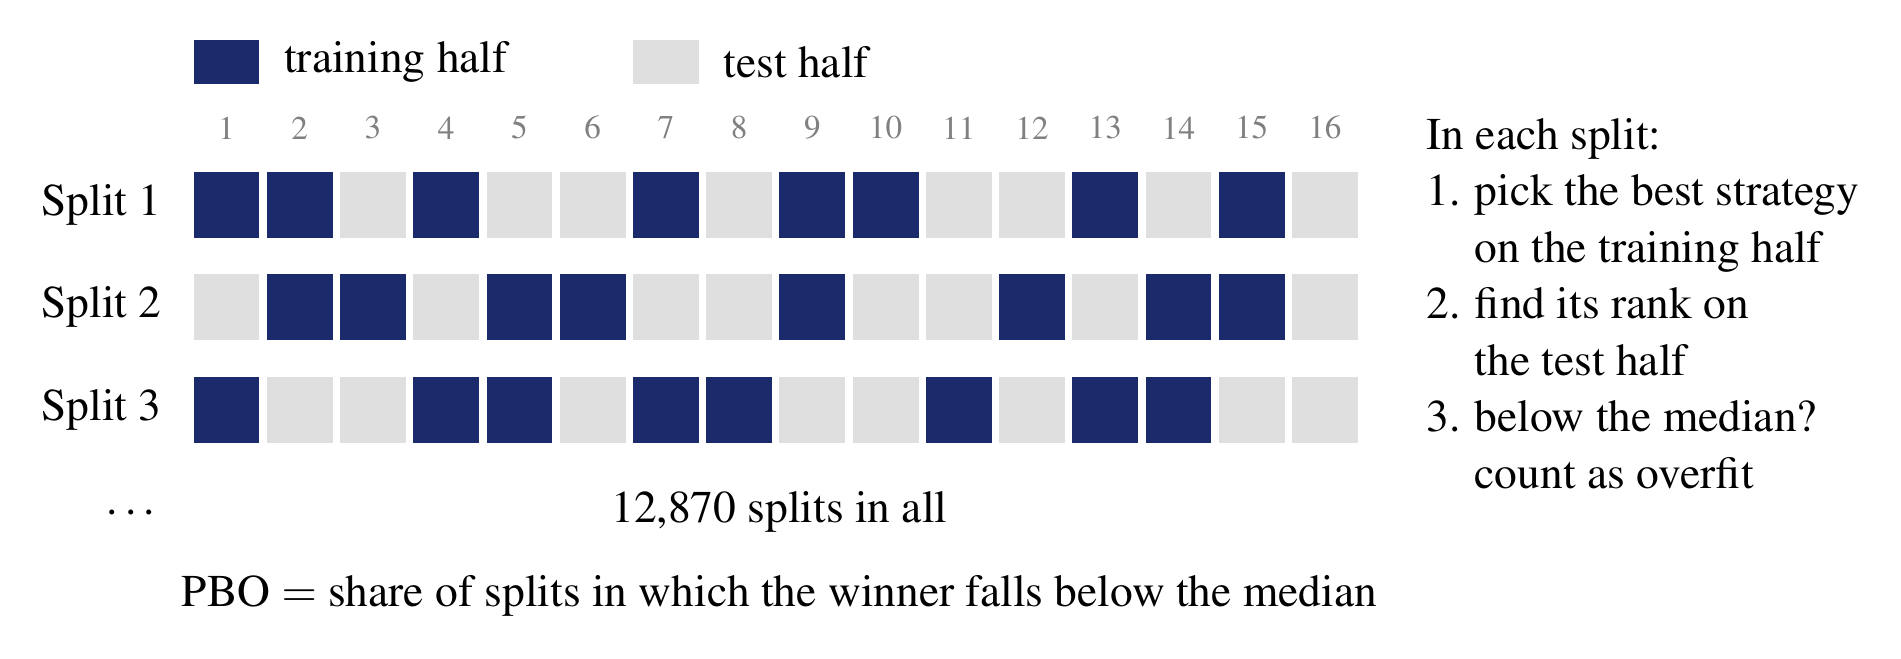
\includegraphics[width=0.9\linewidth]{images/fig04-3-cscv.png}
%\caption{Combinatorially symmetric cross-validation. The sample is cut into 16 blocks. Each split assigns eight blocks to training and eight to testing; every one of the 12,870 possible splits is used. The probability of backtest overfitting is the share of splits in which the training winner ranks below the median in testing.}
%\label{fig:04-cscv}
%\end{figure}

A PBO near 0 means the selection process reliably picks strategies that remain above average; a PBO near 0.5 means in-sample performance carries no information about out-of-sample rank; above 0.5, selection actively picks losers, a sign that the search rewards fitting noise.

CSCV has two advantages over a single train--test split. It uses every observation for both training and testing, and it produces a distribution rather than a single outcome, so one lucky or unlucky split cannot decide the verdict. Its main limitation is that blocks are treated as interchangeable, which ignores the order of time; the lab therefore also reports a conventional chronological out-of-sample test.

\section{Bootstrap reality checks and pre-registration}
\label{sec:04-reality}

\textbf{Reality checks.} White (2000) proposed testing whether the best of many strategies beats a benchmark, using a bootstrap (Section~\ref{sec:03-bootstrap}) that resamples all strategies' returns together and so respects their correlations. Hansen (2005) refined the test, as the superior predictive ability (SPA) test, to make it less sensitive to poor strategies included in the comparison. These tests answer the same question as the deflated Sharpe ratio, but without its distributional approximations.

\begin{callout}
\textbf{What Failed: a century of technical trading rules.} Brock, Lakonishok and LeBaron (1992) found that simple moving-average and trading-range rules applied to the Dow Jones index from 1897 to 1986 produced significant profits. Sullivan, Timmermann and White (1999) re-examined them against a universe of several thousand related rules, using White's reality check to account for the search. The best rule still looked significant in the original sample, but its superior performance did not carry over to the decade that followed. A result that survives a search can still fail the test that matters most: new data.
\end{callout}

\textbf{Pre-registration.} Every correction in this chapter depends on knowing how many trials were run. The surest way to know is to decide in advance. \textbf{Pre-registration} means writing down, before looking at the test data, the hypothesis, the data, the sample period, the strategy's exact rules and the criteria for success, and then reporting the result whatever it is. It is standard in clinical trials and increasingly common in economics. Chapter 25 shows how to write one.

For practitioners without a formal registry, three habits come close:

\begin{enumerate}
  \item \textbf{Keep a trial log.} Record every configuration tested, including those abandoned. It is the input every correction needs.
  \item \textbf{Hold out data you never look at} until the strategy's design is final, and use it once.
  \item \textbf{Prefer economic reasons stated before the test.} A rule motivated by a mechanism is less likely to be an artifact than one found by search and explained afterward.
\end{enumerate}

\section{Lab 4: The best of a thousand rules}
\label{sec:04-lab}

\begin{callout}
\textbf{Lab 4 at a glance.} \emph{Claim on trial:} with the right correction, a broad search can still find strategies that are real. \emph{Data:} monthly U.S. market and Treasury bill returns, from the Kenneth R. French Data Library (Fama/French 3 Factors). \emph{Run time:} under a minute. \emph{Code:} repository folder \texttt{ch04-overfitting/}, with a guided notebook.
\end{callout}

The lab recreates, in miniature, the situation behind the factor zoo. It searches a large family of market-timing rules for the best backtest, then asks whether the winner is a discovery.

\textbf{The rules.} Every rule is either fully in the U.S. stock market or in Treasury bills, and decides at the end of each month for the next. There are 473 rules:

\begin{itemize}
  \item prices above moving averages of 2 to 24 months, with and without bands;
  \item crossovers of fast and slow moving averages;
  \item \textbf{time-series momentum} over 1 to 24 months: holding the market when its own past return is positive;
  \item seasonal rules that leave the market for some months of the year;
  \item a volatility filter.
\end{itemize}

Each also appears in a \textbf{contrarian} version, which does the opposite, for 946 rules in all. Nothing here is exotic. Every rule is the kind of thing a curious analyst might try on a Sunday afternoon.

\textbf{The skill measure.} A rule that is in the market most of the time will earn most of the equity premium, which is not skill (Section~\ref{sec:01-foundations}). The lab therefore scores each rule by its \textbf{hedged return}: the rule's excess return minus its beta times the market's. A rule that always holds the market scores exactly zero. The Sharpe ratio of the hedged return is the rule's \textbf{appraisal ratio}, and its t-statistic is the t-statistic of the rule's alpha.

\textbf{Part A: the search.} The rules are backtested on the first half of the sample, roughly 1929 to 1977. The lab reports how many rules clear each decision rule from Section~\ref{sec:04-corrections}, the best rule's deflated Sharpe ratio with both the raw and the effective number of trials, and then what every rule did in the second half, which played no part in the search.

The effective count needs a way to measure how many independent bets 946 correlated rules contain. The lab's default uses \textbf{principal components}, combinations of the rules' returns ranked by how much of their joint variation each explains, and counts how many are needed to explain 90\% of it. An alternative, the \textbf{participation ratio}, measures how evenly that variation is spread across the components. Half the rules are exact mirror images of the other half, and most trend rules are near copies of each other, so the effective count is far below 946. How far below is a judgment, and one of the exercises asks you to change it and watch the deflated Sharpe ratio move.

\textbf{Part B: overfitting.} CSCV with 16 blocks runs all 12,870 splits of the full sample and reports the PBO and the out-of-sample Sharpe ratio of each split's winner.

\textbf{Part C: the hurdle.} A table and chart of the Sharpe ratio the best of $N$ strategies with no skill is expected to show. With 10 years of monthly data, the best of 100 such strategies is expected to show an annualized Sharpe ratio of about 0.8, and the best of 1,000 about 1.0. With 50 years of data the same searches buy about 0.36 and 0.46. Many backtests offered to investors are shorter than 10 years and rest on more than 100 tries.

\textbf{Part D: what corrections cost.} Here the truth is known. Of 1,000 simulated strategies with 50 years of monthly returns, 100 have a true annualized Sharpe ratio of 0.5 and the rest have none. Across 200 repetitions, the default settings give:

\begin{center}
\small
\begin{tabularx}{0.7\linewidth}{@{}>{\raggedright\arraybackslash}X>{\raggedright\arraybackslash}p{0.26\linewidth}>{\raggedright\arraybackslash}p{0.26\linewidth}@{}}
\toprule
Method & False discovery rate & Good strategies found \\
\midrule
No correction ($t > 1.96$) & 19\% & 94\% \\
$t > 3$ & 1.7\% & 70\% \\
Benjamini--Hochberg & 2.2\% & 74\% \\
Benjamini--Yekutieli & 0.3\% & 47\% \\
Holm & 0.1\% & 31\% \\
Bonferroni & 0.1\% & 31\% \\
\bottomrule
\end{tabularx}
\end{center}

Without a correction, about one discovery in five is false. Bonferroni and Holm almost eliminate false discoveries, but find fewer than a third of the good strategies. Benjamini--Hochberg and the $t > 3$ hurdle keep the false discovery rate low while finding most of them. The exercises change the share of good strategies, their strength and their correlation, and the ranking changes with them.

\textbf{What to look for.} When the lab was tested on simulated market data in which no rule had any skill at all, one draw produced a best rule with a backtest t-statistic of 3.5 and more than 200 rules above 1.96. The rules are correlated, so when luck favors one trend rule it favors hundreds of them together. In that draw the best rule's t-statistic in the second half was $-0.5$, and its deflated Sharpe ratio with all 946 trials was 0.002. Run the lab on real data and see which of these patterns the market's history repeats.

The lab, its tests and a guided notebook are in \texttt{ch04-overfitting} in the book's repository. The README records what has been tested and how.

\section{What investors can use}
\label{sec:04-investors}

The verdict on the claim: \textbf{survives, with conditions.} A broad search can find strategies that are real, but only when three conditions hold:

\begin{enumerate}
  \item \textbf{The hurdle is sized to the search.} A t-statistic of 2 means what textbooks say it means only for a single test decided in advance; after a search it is the expected result of luck, and correlated trials let luck produce many such winners at once. With an honest count of trials, Benjamini--Hochberg or the $t > 3$ hurdle kept false discoveries near 2\% while finding about three-quarters of the good strategies (Part D).
  \item \textbf{The correction matches the decision.} Bonferroni and Holm suit putting all the capital in one strategy; false-discovery-rate methods suit screening a list. Applying the strictest rule everywhere misses most real effects.
  \item \textbf{The winner holds up on data the search never touched}: the second half of the sample in Part A, a low probability of backtest overfitting in Part B, and live performance after the design was fixed.
\end{enumerate}

A search that meets all three is a discovery process. One that reports the best of many tries at $t = 2$ is not.

Five questions turn the chapter into a checklist for any backtest an investor is shown:

\begin{enumerate}
  \item \textbf{How many things were tried?} Ask for the number of strategies, parameter settings, sample periods and variable definitions considered, including those abandoned. A manager who cannot answer has not kept a trial log, and no correction can then be applied.
  \item \textbf{How long is the backtest, relative to that number?} Use the hurdle in Part C. A 10-year backtest with an annualized Sharpe ratio of 1.0 is unremarkable if a thousand variants were tried.
  \item \textbf{Was any data held back?} Ask what part of the history was never used in the design, and when it was first looked at. Live performance after the strategy was fixed is the strongest form of held-back data.
  \item \textbf{Is there a reason stated in advance?} A rule backed by a mechanism that was written down before the test, such as a risk, a friction or a behavioral bias, is more credible than a pattern explained after it was found.
  \item \textbf{How much does performance fall after selection?} Harvey and Liu (2015) proposed \textbf{haircutting} reported Sharpe ratios, cutting them by an amount that reflects the search; McLean and Pontiff (2016) found that published anomalies earned 26\% less in the years between the end of the original sample and publication, and 58\% less after publication. Plan for decay rather than hope against it.
\end{enumerate}

The deeper lesson is about process. The corrections in this chapter repair a search after the fact; pre-registration, trial logs and held-out data prevent the problem from arising. Chapter 25 returns to these as the core of research design, and Chapter 26 asks you to apply them to a project of your own.

\section*{Exercises}
\addcontentsline{toc}{section}{Exercises}

\subsection*{Conceptual (all readers)}

\begin{enumerate}
  \item A researcher tests 50 independent strategies with no skill at the 5\% level. What is the chance that at least one appears significant? How many are expected to appear significant?
  \item Explain in your own words the difference between controlling the family-wise error rate and the false discovery rate. Give one investment decision for which each is the right goal.
  \item Why does the effective number of trials matter for the deflated Sharpe ratio? Give an example of two ``different'' strategies that should count as close to one trial.
  \item A PBO of 0.5 and a PBO of 0.8 both indicate overfitting. What does each tell you about the search that produced them?
\end{enumerate}

\subsection*{Lab extensions (technical readers)}

\begin{enumerate}
  \setcounter{enumi}{4}
  \item Move the split between backtest and holdout to 1963 and then to 2000. Does the same family of rules win each time? Does the winner survive in the later sample?
  \item Re-run Part A with the participation-ratio count of effective trials. How much does the deflated Sharpe ratio change? Write a paragraph arguing who should choose that count, and when.
  \item In Part D, set the correlation between strategies to 0.3, then the share of good strategies to 1\%. When does Benjamini--Hochberg lose control of the false discovery rate, and when does Benjamini--Yekutieli earn its cost?
  \item Add 200 rules of your own, for example the 10-month moving-average rule of Faber (2007) with different bands. How do the best t-statistic, the hurdle and the PBO change? What does this say about adding ``just a few more'' variations?
  \item Implement White's (2000) reality check with the stationary bootstrap of Politis and Romano (1994) from Chapter 3 and apply it to the 946 rules. Compare its verdict with the deflated Sharpe ratio's.
  \item Choose a published anomaly from the Chen and Zimmermann (2022) data set. Estimate how many related variables and sample choices its authors might plausibly have considered, and judge whether its t-statistic clears the corresponding hurdle.
\end{enumerate}

\section*{References}
\addcontentsline{toc}{section}{References}

\begin{itemize}
  \item Bailey, D. H., Borwein, J. M., L\'opez de Prado, M. and Zhu, Q. J. (2014). Pseudo-Mathematics and Financial Charlatanism: The Effects of Backtest Overfitting on Out-of-Sample Performance. \emph{Notices of the American Mathematical Society} 61(5): 458--471.
  \item Bailey, D. H., Borwein, J. M., L\'opez de Prado, M. and Zhu, Q. J. (2017). The Probability of Backtest Overfitting. \emph{Journal of Computational Finance} 20(4): 39--69.
  \item Bailey, D. H. and L\'opez de Prado, M. (2012). The Sharpe Ratio Efficient Frontier. \emph{Journal of Risk} 15(2): 3--44.
  \item Bailey, D. H. and L\'opez de Prado, M. (2014). The Deflated Sharpe Ratio: Correcting for Selection Bias, Backtest Overfitting, and Non-Normality. \emph{Journal of Portfolio Management} 40(5): 94--107.
  \item Benjamin, D. J., Berger, J. O., Johannesson, M., Nosek, B. A., Wagenmakers, E.-J., et al. (2018). Redefine Statistical Significance. \emph{Nature Human Behaviour} 2(1): 6--10.
  \item Benjamini, Y. and Hochberg, Y. (1995). Controlling the False Discovery Rate: A Practical and Powerful Approach to Multiple Testing. \emph{Journal of the Royal Statistical Society: Series B} 57(1): 289--300.
  \item Benjamini, Y. and Yekutieli, D. (2001). The Control of the False Discovery Rate in Multiple Testing under Dependency. \emph{Annals of Statistics} 29(4): 1165--1188.
  \item Brock, W., Lakonishok, J. and LeBaron, B. (1992). Simple Technical Trading Rules and the Stochastic Properties of Stock Returns. \emph{Journal of Finance} 47(5): 1731--1764.
  \item Chen, A. Y. and Zimmermann, T. (2022). Open Source Cross-Sectional Asset Pricing. \emph{Critical Finance Review} 11(2): 207--264.
  \item Cochrane, J. H. (2011). Presidential Address: Discount Rates. \emph{Journal of Finance} 66(4): 1047--1108.
  \item Faber, M. T. (2007). A Quantitative Approach to Tactical Asset Allocation. \emph{Journal of Wealth Management} 9(4): 69--79.
  \item Hansen, P. R. (2005). A Test for Superior Predictive Ability. \emph{Journal of Business and Economic Statistics} 23(4): 365--380.
  \item Harvey, C. R. (2017). Presidential Address: The Scientific Outlook in Financial Economics. \emph{Journal of Finance} 72(4): 1399--1440.
  \item Harvey, C. R. and Liu, Y. (2015). Backtesting. \emph{Journal of Portfolio Management} 42(1): 13--28.
  \item Harvey, C. R. and Liu, Y. (2020). False (and Missed) Discoveries in Financial Economics. \emph{Journal of Finance} 75(5): 2503--2553.
  \item Harvey, C. R., Liu, Y. and Zhu, H. (2016). \ldots and the Cross-Section of Expected Returns. \emph{Review of Financial Studies} 29(1): 5--68.
  \item Holm, S. (1979). A Simple Sequentially Rejective Multiple Test Procedure. \emph{Scandinavian Journal of Statistics} 6(2): 65--70.
  \item Hou, K., Xue, C. and Zhang, L. (2020). Replicating Anomalies. \emph{Review of Financial Studies} 33(5): 2019--2133.
  \item Jensen, T. I., Kelly, B. and Pedersen, L. H. (2023). Is There a Replication Crisis in Finance? \emph{Journal of Finance} 78(5): 2465--2518.
  \item Lo, A. W. (2002). The Statistics of Sharpe Ratios. \emph{Financial Analysts Journal} 58(4): 36--52.
  \item Lo, A. W. and MacKinlay, A. C. (1990). Data-Snooping Biases in Tests of Financial Asset Pricing Models. \emph{Review of Financial Studies} 3(3): 431--467.
  \item L\'opez de Prado, M. (2019). A Data Science Solution to the Multiple-Testing Crisis in Financial Research. \emph{Journal of Financial Data Science} 1(1): 99--110.
  \item McLean, R. D. and Pontiff, J. (2016). Does Academic Research Destroy Stock Return Predictability? \emph{Journal of Finance} 71(1): 5--32.
  \item Moskowitz, T. J., Ooi, Y. H. and Pedersen, L. H. (2012). Time Series Momentum. \emph{Journal of Financial Economics} 104(2): 228--250.
  \item Politis, D. N. and Romano, J. P. (1994). The Stationary Bootstrap. \emph{Journal of the American Statistical Association} 89(428): 1303--1313.
  \item Sullivan, R., Timmermann, A. and White, H. (1999). Data-Snooping, Technical Trading Rule Performance, and the Bootstrap. \emph{Journal of Finance} 54(5): 1647--1691.
  \item White, H. (2000). A Reality Check for Data Snooping. \emph{Econometrica} 68(5): 1097--1126.
\end{itemize}

\textbf{Data:} Kenneth R. French Data Library: Fama/French 3 Factors (monthly). \url{https://mba.tuck.dartmouth.edu/pages/faculty/ken.french/data_library.html}

% Chapter 5 -- Out-of-Sample Design and Forecast Evaluation
% Requires: amsmath, amssymb, booktabs, array, tabularx, graphicx, tcolorbox (breakable, skins), hyperref or url.
% Defines the callout box only if the preamble has not.
\providecolor{fenavy}{HTML}{1B2A6B}
\providecolor{feshade}{HTML}{F3F5FA}
\makeatletter
\@ifundefined{callout}{%
  \newtcolorbox{callout}{breakable, enhanced,
    colback=white, colframe=gray!70, boxrule=0.5pt, arc=1mm,
    borderline west={2.5pt}{0pt}{gray!70},
    left=8pt, right=8pt, top=4pt, bottom=4pt}%
}{}
\makeatother

\chapter{Out-of-Sample Design and Forecast Evaluation}
\label{ch:05}

Chapter 4 asked how strong the evidence must be when many strategies are tried. This chapter asks a different question about a single model: does it forecast, or did it only fit?

A regression estimated on the whole history of the data has seen every observation it is judged on. Its $R^2$ measures how well it describes the past, with the benefit of hindsight about which way the coefficients should point and how large they should be. A forecaster has no such benefit. At each date she knows only what had happened up to then, must estimate her model from that, and is judged on what happens next.

The claim on trial is one that most empirical finance took for granted until the mid-2000s: \textbf{a predictor that fits well in-sample will forecast well out of sample.}

By the end of the chapter you will be able to:

\begin{itemize}
  \item explain point forecasts, loss functions and information sets, and measure accuracy with the mean squared error;
  \item explain the bias--variance trade-off and why simple models often forecast better than rich ones;
  \item distinguish training, validation and test data, and explain why time series must be split in order;
  \item describe autoregressive models and persistence, and explain why in-sample $R^2$ flatters complex models;
  \item design a walk-forward evaluation that uses only information available at each forecast date, with expanding or rolling windows;
  \item recognize and remove the common forms of leakage, including the overlapping-target leak that purging and embargoing prevent;
  \item choose a benchmark that is hard to beat, and measure performance against it with the out-of-sample $R^2$ and the Clark--West and Diebold--Mariano tests;
  \item judge forecasts by their economic value and, for probabilistic forecasts, with proper scoring rules;
  \item explain why a predictor that truly works can still fail out of sample, and why one that fails can still be real.
\end{itemize}

In the lab you will take 14 variables that published research has used to predict the U.S. stock market, the data set of Goyal and Welch (2008), and ask each to forecast month by month from 1965 using only what was known at the time. A simulation in which the truth is known then shows how often each test reaches the right verdict.

\section{Foundations: the basics of forecasting}
\label{sec:05-foundations}

\textbf{Point forecasts and loss functions.} A \textbf{point forecast} is a single number: the forecaster's best guess of next month's return. ``Best'' depends on a \textbf{loss function} that says how costly each error is.

\begin{itemize}
  \item Under \textbf{squared-error loss}, an error of 2 costs four times as much as an error of 1. The best forecast is then the \textbf{conditional mean}, the average outcome given everything known at the time. Accuracy is measured by the \textbf{mean squared error} (MSE), the average of the squared forecast errors, or its square root (RMSE), which is in the same units as the forecast.
  \item Under absolute-error loss, an error of 2 costs twice as much as an error of 1, and the best forecast is the median.
\end{itemize}

Finance mostly uses squared error, because it connects directly to variance and to mean--variance portfolio choice.

\textbf{Information sets.} A forecast made at time $t$ may use only the \textbf{information set} available at $t$: past prices, published data, and models estimated on past observations. Everything in this chapter follows from enforcing that rule.

\textbf{The bias--variance trade-off.} A forecast's expected squared error has three parts (Figure~\ref{fig:05-biasvar}):

\begin{itemize}
  \item the irreducible \textbf{noise} in the outcome, which no model can remove;
  \item the \textbf{bias} from a model that is systematically wrong, for example because it leaves out a real effect;
  \item the \textbf{variance} from estimating the model on a finite sample: a different sample would give different coefficients and different forecasts.
\end{itemize}

Richer models, with more parameters, reduce bias but increase variance. When the signal is weak relative to the noise, as for stock returns, a simple model with few parameters often forecasts better than a rich one, even if the rich one is closer to the truth. Fitting the noise in a sample instead of the signal is called \textbf{overfitting}.

\providecolor{fenavy}{HTML}{1B2A6B}
\providecolor{fegray}{HTML}{4D4D4D}

\begin{figure}[htbp]
  \centering
  \begin{tikzpicture}[
    declare function={
      bias(\x)  = 0.67/(\x + 0.47);   % squared bias: falls with complexity
      var(\x)   = 0.0048*\x^2.16;     % variance: rises with complexity
      noise     = 0.14;               % irreducible noise
    }]
  \begin{axis}[
    width=0.85\linewidth, height=0.52\linewidth,
    axis lines=left,
    axis line style={-stealth, thin},
    xmin=0, xmax=10.3, ymin=0, ymax=1.08,
    xtick=\empty, ytick=\empty,
    xlabel={Model complexity (number of parameters)},
    ylabel={Expected forecast error},
    samples=200,
    clip=false,
  ]
    % Components
    \addplot[fegray, thick, dashed, domain=0.24:10] {bias(x)};
    \addplot[fegray, thick, densely dotted, domain=0:10] {var(x)};
    \addplot[gray, thin, domain=0:10] {noise};
    % Total = bias + variance + noise
    \addplot[fenavy, very thick, domain=0.27:10] {bias(x) + var(x) + noise};

    % Best point
    \draw[fenavy, densely dashed, thin] (axis cs:3.45,0) -- (axis cs:3.45,0.381);
    \node[fenavy, anchor=south] at (axis cs:3.45,0.47) {best};

    % Right-hand labels
    \node[fenavy, anchor=west] at (axis cs:10.1,0.898) {total error};
    \node[fegray, anchor=west] at (axis cs:10.1,0.694) {variance};
    \node[gray,   anchor=west] at (axis cs:10.1,0.16)  {noise};
    \node[fegray, anchor=west] at (axis cs:10.1,0.05) {bias};

    % Regions
    \node[anchor=west] at (axis cs:0.6,1.0)  {underfit};
    \node[anchor=west] at (axis cs:7.3,0.53) {overfit};
  \end{axis}
  \end{tikzpicture}
  \caption{The bias--variance trade-off. Adding parameters lowers bias but
    raises the variance that comes from estimating them. Total forecast error
    is lowest at an intermediate complexity. When the signal is weak, as for
    stock returns, the best point lies far to the left.}
  \label{fig:05-biasvar}
\end{figure}

%\begin{figure}[htbp]
%\centering
%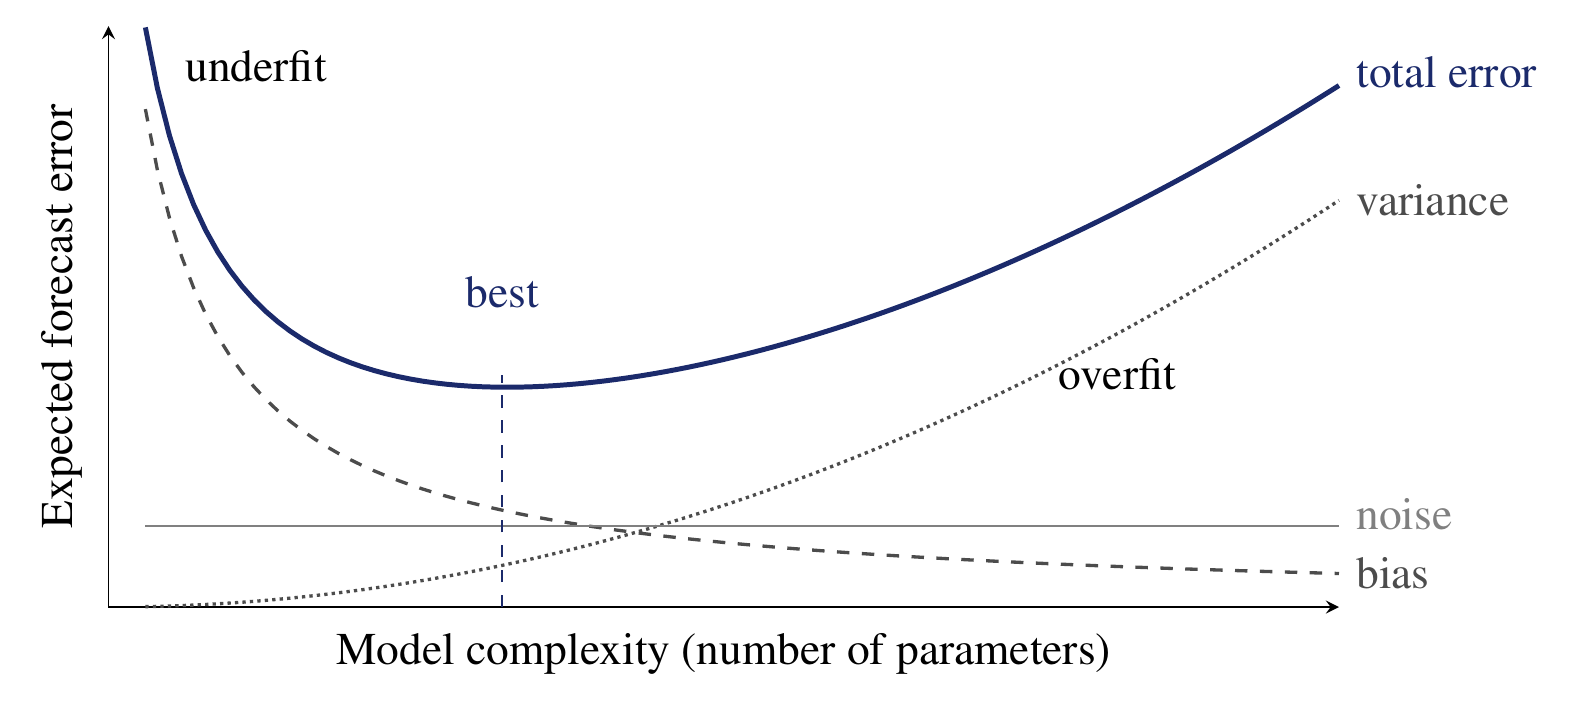
\includegraphics[width=0.85\linewidth]{images/fig05-1-bias-variance.png}
%\caption{The bias--variance trade-off. Adding parameters lowers bias but raises the variance that comes from estimating them. Total forecast error is lowest at an intermediate complexity. When the signal is weak, as for stock returns, the best point lies far to the left.}
%\label{fig:05-biasvar}
%\end{figure}

\textbf{Training, validation and test data.} Machine learning separates data into three parts:

\begin{itemize}
  \item a \textbf{training set} to estimate the model;
  \item a \textbf{validation set} to choose among models or tune settings;
  \item a \textbf{test set}, used once, to measure performance.
\end{itemize}

In time series the order matters: the training data must come before the test data, so random splits used for independent observations are not valid.

\textbf{Autoregressive models.} The simplest time-series forecasting model predicts a variable from its own past. The \textbf{first-order autoregressive model}, AR(1), is
\begin{equation}
  y_{t+1} = c + \phi\,y_t + \varepsilon_{t+1}
  \label{eq:05-ar1}
\end{equation}
The parameter $\phi$ measures \textbf{persistence}: values near 1 mean the series moves slowly, like interest rates or valuation ratios; values near 0 mean it is close to unpredictable, like stock returns. A \textbf{predictive regression} replaces $y_t$ on the right with another variable $x_t$ believed to carry information about $y_{t+1}$.

\textbf{In-sample $R^2$.} For a regression estimated on the data it is judged on,
\begin{equation}
  R^2 = 1 - \frac{\text{sum of squared residuals}}{\text{total sum of squares}}
  \label{eq:05-r2}
\end{equation}
where the total sum of squares measures how far the outcomes vary around their own mean. This $R^2$ can never be negative, and adding variables can never reduce it. This is why in-sample fit flatters complex models.

\textbf{Worked example.} A model with an in-sample $R^2$ of 2\% on monthly returns explains 2\% of the variance of returns. If returns have a monthly standard deviation of 4.5\%, the model's forecasts vary with a standard deviation of only about $\sqrt{0.02} \times 4.5\% \approx 0.6\%$ a month, small next to the noise in any single month.

\textbf{Further reading.} Hyndman and Athanasopoulos, \emph{Forecasting: Principles and Practice} (free online), chapters on forecast evaluation and time-series cross-validation; Diebold, \emph{Forecasting in Economics, Business, Finance and Beyond} (free online); Hastie, Tibshirani and Friedman, \emph{The Elements of Statistical Learning}, chapter on model assessment and selection.

\section{In-sample fit versus out-of-sample performance}
\label{sec:05-insample}

The standard test of return predictability is a regression of next period's excess return on a variable known today:
\begin{equation}
  r_{t+1} = \alpha + \beta x_t + \varepsilon_{t+1}
  \label{eq:05-pred}
\end{equation}

If $\beta$ is significantly different from zero, $x$ is said to predict returns. Fama and French (1988) and Campbell and Shiller (1988) used regressions like this to argue that the dividend--price ratio predicts stock returns, and dozens of other variables followed: interest rates, yield spreads, inflation, the volume of share issuance, measures of risk. By the early 2000s, predictability of the equity premium was widely regarded as a stylized fact.

Goyal and Welch (2008) asked a simple question of these predictors. Suppose an investor in 1965 had used each one, estimating the regression with data only up to the forecast date and re-estimating it every month. Would she have forecast better than someone who simply used the average past return? For most predictors the answer was no. Many that were significant in-sample produced out-of-sample forecasts worse than the historical mean, and the few that helped did so only in some decades. Their 2024 update with Zafirov found the same pattern for predictors proposed since.

Three forces open the gap between fit and forecast.

\textbf{Estimation error.} A forecaster must estimate $\alpha$ and $\beta$ from a finite sample, and the errors in those estimates become errors in her forecasts. When the true predictable share of returns is tiny, as it is for monthly stock returns, this noise can outweigh the signal. As a rough guide, estimating one extra slope from $n$ months of data costs about $1/n$ of $R^2$: with 40 years of monthly data, $n = 480$, about 0.2\%. The best equity-premium predictors are thought to explain perhaps 0.5\% to 1\% of monthly variation. The margin is thin.

\textbf{Instability.} Relationships in markets change. A predictor may work in one era and not another because the economy changes, because investors learn, or because the predictor itself was an artifact of one period. An in-sample regression averages over all eras; a forecaster lives through them in order.

\textbf{Selection.} Chapter 4's problem returns in a quieter form. Predictors that appear in the literature were selected partly because they fit the data their discoverers had. That fit is partly luck, and luck does not repeat.

A fourth problem inflates in-sample evidence itself. Most popular predictors, such as valuation ratios and interest rates, are highly persistent, and their surprises are correlated with return surprises. Stambaugh (1999) showed that this biases the estimated slope in finite samples and makes conventional t-statistics too large. Chapter 3's lab demonstrated the related problem of overlapping long-horizon regressions.

\textbf{Out-of-sample tests are not automatically better.} Inoue and Kilian (2004) pointed out that in-sample tests are more powerful: they use all the data to estimate the parameters, while out-of-sample tests spend part of the sample on training. A predictor can be genuine and still fail out of sample because the test lacks power. The value of out-of-sample evaluation is not that it is more accurate in theory, but that it is harder to fool: it guards against data mining, against hindsight in the choice of specification, and against relationships that have broken down. This chapter's lab measures both sides of that trade-off.

\section{Walk-forward evaluation: expanding and rolling windows}
\label{sec:05-walkforward}

A \textbf{walk-forward} (or recursive) evaluation replays history as a forecaster would have lived it:

\begin{enumerate}
  \item Choose a first forecast date, leaving enough earlier data to estimate the model.
  \item Estimate the model using only data available at that date.
  \item Forecast the next period, and record the forecast and the benchmark's forecast.
  \item Move forward one period, add the new observation, and repeat.
\end{enumerate}

The result is a series of genuine forecasts, each made without knowledge of what followed. Evaluation statistics are computed on this series alone.

The main design choice is which past data to use at each step (Figure~\ref{fig:05-windows}):

\begin{center}
\small
\begin{tabularx}{0.9\linewidth}{@{}>{\raggedright\arraybackslash}p{0.13\linewidth}>{\raggedright\arraybackslash}X>{\raggedright\arraybackslash}p{0.24\linewidth}>{\raggedright\arraybackslash}p{0.24\linewidth}@{}}
\toprule
Window & Training data at each date & Strength & Weakness \\
\midrule
Expanding & All data from the start of the sample & Most data, lowest estimation error & Slow to adapt if the relationship changes \\
Rolling & The most recent $w$ periods only & Adapts to change & More estimation error; results depend on $w$ \\
Fixed & One training period, never updated & Simplest; mimics a model frozen at launch & Ignores new information \\
\bottomrule
\end{tabularx}
\end{center}

\providecolor{fenavy}{HTML}{1B2A6B}

\begin{figure}[htbp]
  \centering
  \begin{tikzpicture}[
    x=0.36cm, y=0.5cm,
    est/.style={fill=fenavy!18, draw=white, line width=0.6pt},
    fc/.style={fill=fenavy, draw=white, line width=0.6pt},
    lab/.style={anchor=east, font=\small},
    head/.style={anchor=west, font=\small\bfseries},
  ]
    \def\wfOff{16}  % horizontal start of the right-hand panel

    % ---------- Expanding window (left) ----------
    \node[head] at (0,1.2) {Expanding window};
    \foreach \wfS in {1,...,5} {
      \pgfmathsetmacro{\wfY}{-\wfS+1}
      \node[lab] at (-0.3,\wfY) {Step \wfS};
      \fill[est] (0,\wfY-0.3) rectangle (8+\wfS,\wfY+0.3);
      \fill[fc]  (8+\wfS,\wfY-0.3) rectangle (9+\wfS,\wfY+0.3);
    }

    % ---------- Rolling window (right) ----------
    \node[head] at (\wfOff,1.2) {Rolling window};
    \foreach \wfS in {1,...,5} {
      \pgfmathsetmacro{\wfY}{-\wfS+1}
      \fill[est] (\wfOff+\wfS-1,\wfY-0.3) rectangle (\wfOff+8+\wfS,\wfY+0.3);
      \fill[fc]  (\wfOff+8+\wfS,\wfY-0.3) rectangle (\wfOff+9+\wfS,\wfY+0.3);
    }

    % Time axis under both panels
    \draw[-stealth, thin] (0,-5) -- (\wfOff+15.2,-5)
      node[anchor=west, font=\small] {time};

    % Legend
    \fill[est] (4,-6.35) rectangle (5.5,-5.65);
    \node[anchor=west, font=\small] at (5.8,-6) {training data};
    \fill[fc]  (\wfOff,-6.35) rectangle (\wfOff+1.5,-5.65);
    \node[anchor=west, font=\small] at (\wfOff+1.8,-6) {forecast period};
  \end{tikzpicture}
  \caption{Walk-forward evaluation. At each step the model is estimated on the
    light bar and forecasts the dark one; then the evaluation moves forward one
    period. An expanding window keeps all past data; a rolling window keeps a
    fixed length and drops the oldest observations.}
  \label{fig:05-windows}
\end{figure}

%\begin{figure}[htbp]
%\centering
%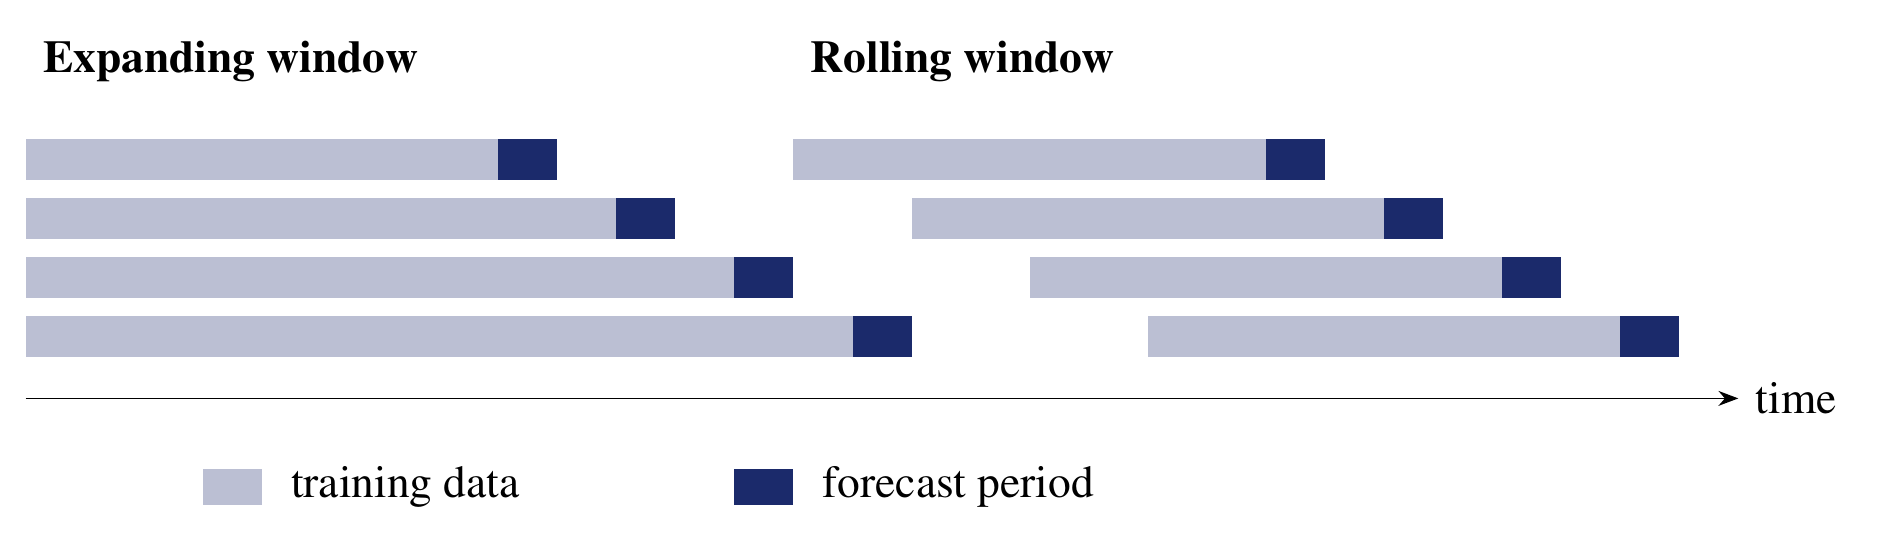
\includegraphics[width=0.9\linewidth]{images/fig05-2-walk-forward.png}
%\caption{Walk-forward evaluation. At each step the model is estimated on the light bar and forecasts the dark one; then the evaluation moves forward one period. An expanding window keeps all past data; a rolling window keeps a fixed length and drops the oldest observations.}
%\label{fig:05-windows}
%\end{figure}

No window is right in general. The choice is a bet on whether the relationship is stable (favoring expanding windows) or changing (favoring rolling ones). The danger is choosing the window after seeing which one works best: that is a search, and Chapter 4 applies. Decide the window, the first forecast date and the minimum training period before looking at the results, and report sensitivity to the alternatives.

\textbf{Restrictions from theory.} Campbell and Thompson (2008) showed that two simple restrictions, motivated by economics rather than statistics, improve many predictors' out-of-sample performance:

\begin{itemize}
  \item if the estimated slope has the opposite sign to the one theory predicts, use the historical mean instead;
  \item never forecast a negative equity premium, since investors would not hold stocks expecting to lose.
\end{itemize}

Restrictions like these reduce estimation error by ruling out implausible forecasts. They are legitimate if fixed in advance, and a form of search if chosen afterward.

\textbf{Re-estimation is part of the model.} In machine-learning applications the same logic covers every choice fitted to data: hyperparameters, \textbf{feature selection} (choosing which input variables to use), the choice among models. All must be redone inside each training window, using only that window's data. A model whose hyperparameters were tuned on the full sample has seen the test data, however carefully its coefficients were estimated.

\section{Leakage: look-ahead, publication lags, purging and embargoing}
\label{sec:05-leakage}

\textbf{Leakage} is any route by which information from the test period reaches the model or the evaluation. It is the most common reason a backtest looks better than live trading, and it rarely announces itself. The forms worth checking for are these.

\textbf{Full-sample estimation.} The classic error is to estimate a model on the whole sample and then ``test'' it on part of the same sample. The coefficients already know how the test period turned out. The same applies to anything fitted: standardizing variables with full-sample means and standard deviations, choosing lags, or \textbf{winsorizing}, capping extreme values at chosen percentiles, when those percentiles come from the full sample.

\textbf{Hindsight in choosing the model.} Choosing which predictor to use, or which of several models, because it performed well over the whole sample is look-ahead even if each model is then evaluated walk-forward. The honest version makes the choice at each date using only past data.

\textbf{Publication lags and revisions.} A variable dated March is not necessarily known in March. Consumer prices for March are published in April; company earnings for a quarter arrive weeks or months later; many macroeconomic series are revised for years after first release. Using the final, revised value as if it had been known on its reference date is leakage. Goyal and Welch lag inflation by an extra month for this reason. For macroeconomic predictors, real-time vintages such as the Federal Reserve Bank of St.\ Louis's ALFRED archive record what was known when. Chapter 2's discussion of point-in-time data (Section~\ref{sec:02-lookahead}) applies throughout.

\textbf{Overlapping targets.} Suppose the target is the return over the next 12 months. The observation formed in June has a target that runs through the following June. If the model is trained at the end of December on all observations up to November, the last eleven of them have targets that include returns after December, which the forecaster could not have known. A walk-forward evaluation must therefore drop those observations from training (Figure~\ref{fig:05-purging}). L\'opez de Prado (2018) calls this \textbf{purging}: removing from the training set every observation whose target overlaps the test period.

\providecolor{fenavy}{HTML}{1B2A6B}

\begin{figure}[htbp]
  \centering
  \begin{tikzpicture}[
    x=0.28cm, y=0.42cm,
    lab/.style={anchor=west, font=\small, align=left},
  ]
    % Months relative to the forecast date (0). Each observation is formed at
    % month m and paired with the 12-month return from m to m+12.

    % Kept: target ends before the forecast date
    \foreach \wfM [count=\wfR from 0] in {-17,-15,-13} {
      \draw[fenavy, thick] (\wfM,\wfR) -- (\wfM+12,\wfR);
      \fill[fenavy] (\wfM,\wfR) circle (2.6pt);
    }

    % Purged: target runs past the forecast date
    \foreach \wfM [count=\wfR from 3] in {-11,-9,-7,-5,-3,-1} {
      \draw[gray!55, densely dashed] (\wfM,\wfR) -- (\wfM+12,\wfR);
      \fill[gray!55] (\wfM,\wfR) circle (2.6pt);
    }

    % Forecast date
    \draw[fenavy, thick] (0,-1.5) -- (0,8.6);
    \node[fenavy, font=\small, anchor=south, align=center] at (0,8.6)
      {forecast date\\(end of December)};

    % Time axis
    \draw[-stealth, thin] (-18.5,-1) -- (13,-1)
      node[anchor=west, font=\small] {months};

    % Labels
    \node[lab, gray] at (13.5,7) {purged: target runs\\past the forecast date};
    \node[lab, fenavy] at (1.2,0.7) {kept: 12-month target\\ends before the forecast};
    \node[font=\small, gray!40!black, anchor=north, align=center]
      at (-9,-1.6) {training observations (dot $=$ date formed;\\
                    line $=$ 12-month return it is trained to predict)};
  \end{tikzpicture}
  \caption{Purging. Each training observation is paired with the 12-month
    return that follows it. Observations whose 12-month target runs past the
    forecast date (dashed) contain returns the forecaster could not yet know,
    so they are removed from the training set.}
  \label{fig:05-purging}
\end{figure}

%\begin{figure}[htbp]
%\centering
%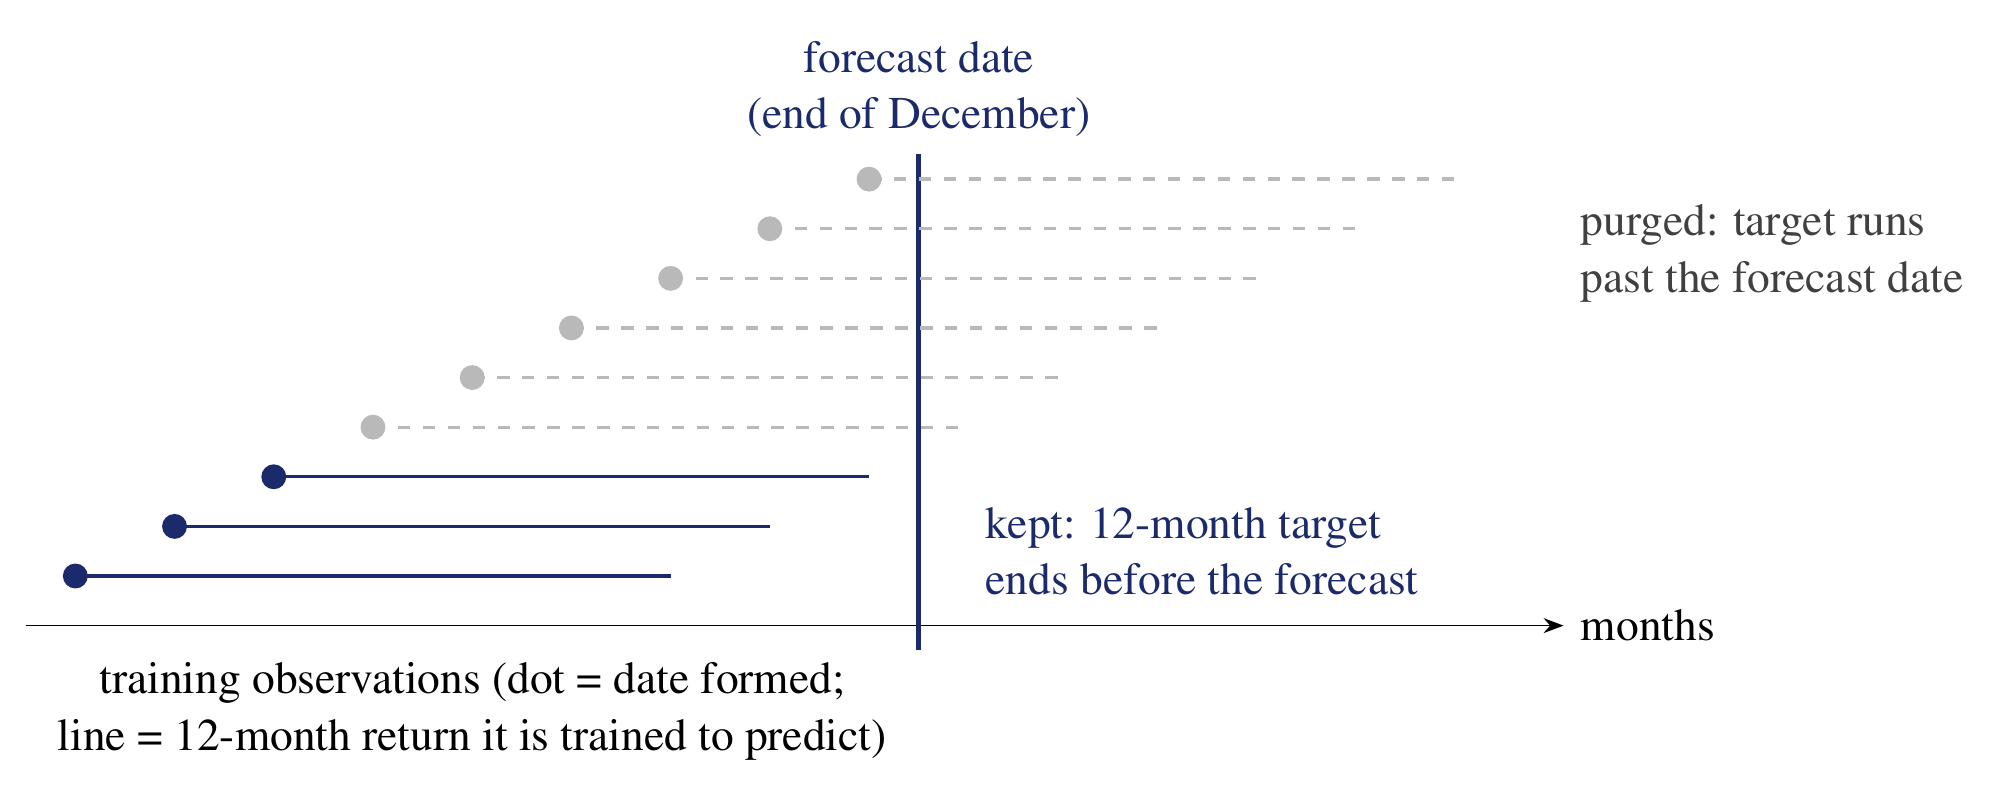
\includegraphics[width=0.85\linewidth]{images/fig05-3-purging.png}
%\caption{Purging. Each training observation is paired with the 12-month return that follows it. Observations whose 12-month target runs past the forecast date (dashed) contain returns the forecaster could not yet know, so they are removed from the training set.}
%\label{fig:05-purging}
%\end{figure}

\textbf{Serial correlation across the boundary.} When training data can come after the test period, as in the cross-validation of Chapter 4, observations just after the test period may still carry information about it through serially correlated features. L\'opez de Prado's \textbf{embargo} drops a short period of training data immediately after each test block. In a pure walk-forward design, where training always precedes testing, purging is needed but an embargo is not.

\textbf{Survivorship and selection in the data.} Datasets of current index members, surviving funds or listed firms build in knowledge of who survived. Chapter 2 covered these traps; they matter as much for forecasting as for backtesting.

Lab 5 measures several of these leaks on real data, comparing each with its honest counterpart.

\section{Benchmarks that are hard to beat}
\label{sec:05-benchmarks}

A forecast is only as impressive as the alternative it beats. Choosing a weak benchmark, such as zero, or a model nobody would use, is one of the easiest ways to make a forecasting method look good. The benchmarks that matter are the simple ones a sensible person would use without any model at all.

\begin{center}
\small
\begin{tabularx}{0.9\linewidth}{@{}>{\raggedright\arraybackslash}p{0.18\linewidth}>{\raggedright\arraybackslash}p{0.28\linewidth}>{\raggedright\arraybackslash}X@{}}
\toprule
Quantity forecast & Natural benchmark & Why it is hard to beat \\
\midrule
Equity premium & Historical mean of past returns & Only one parameter to estimate; no exposure to unstable relationships \\
Exchange rates, asset prices & Random walk: tomorrow equals today & Meese and Rogoff (1983) found that structural exchange-rate models did not beat it, a result that has proved durable \\
Interest rates, yields & Random walk, or the forward rate & Rates are highly persistent; Chapter 16 tests the forward rate as a forecast \\
Volatility & Recent realized volatility, or a simple exponentially weighted average & Volatility clusters, so the recent past is informative; Chapter 11 tests richer models \\
Macroeconomic series & Survey consensus, or the last value & Professional forecasters already use most public information \\
\bottomrule
\end{tabularx}
\end{center}

An \textbf{exponentially weighted average} gives the most weight to the latest observation and steadily less to older ones. A \textbf{survey consensus} is the average forecast of professional forecasters.

The historical mean is the benchmark for the equity premium because it is what an investor would assume without a forecasting model. It is computed in real time, with the same training data as the model, so that the comparison isolates the value of the predictor. Beating it is hard for the reason given in Section~\ref{sec:05-insample}: the predictor's signal is small and its estimation error is not.

A useful habit is to name the benchmark before building the model, and to ask what a skeptical colleague would accept as the default. If a new method cannot beat that default, its sophistication is a cost rather than a benefit.

\section{Measuring forecast accuracy: out-of-sample $R^2$, Diebold--Mariano and Clark--West}
\label{sec:05-accuracy}

\textbf{The out-of-sample $R^2$.} Campbell and Thompson (2008) summarized forecast accuracy against the historical mean with
\begin{equation}
  R^2_{OS} = 1 - \frac{\sum_t (r_{t+1} - \hat r_{t+1})^2}{\sum_t (r_{t+1} - \bar r_{t})^2}
  \label{eq:05-r2os}
\end{equation}
where $\hat r_{t+1}$ is the model's forecast and $\bar r_t$ the historical mean, both computed from data up to $t$. Unlike the in-sample $R^2$ of Equation~\eqref{eq:05-r2}, it can be negative, and it is negative whenever the model's squared errors exceed the benchmark's. Positive values are small in this field. For monthly stock returns, an out-of-sample $R^2$ of 0.5\% would be a good result.

Goyal and Welch (2008) added a picture that is often more revealing than any summary statistic: the cumulative difference between the benchmark's squared errors and the model's, plotted over time. A line that rises steadily indicates a model that keeps winning; one that rises in a single episode and then drifts sideways or down indicates a result that depends on one period.

\textbf{Is the difference significant?} Diebold and Mariano (1995) proposed testing whether two forecasts are equally accurate by looking at the series of differences in their losses,
\begin{equation}
  d_t = e^2_{\text{bench},t} - e^2_{\text{model},t}
  \label{eq:05-dm}
\end{equation}
where $e$ denotes a forecast error. If the forecasts are equally accurate, $d_t$ has mean zero; a t-test on its mean, with Newey--West standard errors for multi-step forecasts (Section~\ref{sec:03-se}), gives the test. Harvey, Leybourne and Newbold (1997) proposed a small-sample correction that is now standard.

\textbf{The nested-model problem.} Two models are \textbf{nested} when one is a special case of the other. The DM test was designed for competing forecasts. When the model contains the benchmark as a special case, as a predictive regression contains the historical mean (set $\beta = 0$), the test misbehaves. Under the null that $\beta = 0$, the larger model still estimates $\beta$, and the estimation noise makes its forecasts slightly worse on average. The DM statistic is then centered below zero, and the test rejects too rarely. Clark and West (2007) proposed an adjustment that adds back the expected cost of that noise:
\begin{equation}
  f_t = (r_{t+1} - \bar r_t)^2 - \left[(r_{t+1} - \hat r_{t+1})^2 - (\bar r_t - \hat r_{t+1})^2\right]
  \label{eq:05-cw}
\end{equation}
and a one-sided t-test on the mean of $f_t$. It is the standard test for the equity-premium literature, and the lab reports it alongside DM. Note the asymmetry: Clark--West can declare a model significantly informative even when its out-of-sample $R^2$ is slightly negative, because it asks whether the predictor carries information, not whether this particular estimated forecast beat the mean.

\textbf{Economic value.} Statistical accuracy and economic value are not the same thing. Campbell and Thompson showed that an investor who times the market can gain substantially from an $R^2$ that looks negligible. Roughly, a market timer's expected excess return rises in proportion to $R^2/S^2$, where $S$ is the market's Sharpe ratio per period. With a monthly Sharpe ratio of about 0.12 (0.42 a year) and a monthly $R^2$ of 0.5\%, the ratio is $0.005/0.12^2 \approx 0.35$: the timer's expected excess return rises by about a third.

The lab measures economic value directly. A \textbf{mean--variance investor}, who cares only about the mean and variance of her portfolio's return, uses each forecast to set her equity weight, and the result is compared with the same investor using the historical mean. The difference is reported as a gain in \textbf{certainty-equivalent return}: the riskless return she would accept instead of the risky strategy. This translates a forecast into the unit an investor cares about, but it depends on the investor's \textbf{risk aversion}, how much expected return she demands per unit of variance, and on the limits placed on her weights, so those choices should also be fixed in advance.

\section{Probabilistic forecasts and proper scoring rules}
\label{sec:05-scoring}

Much of finance needs more than a single number. A risk manager needs the probability of a large loss; an option trader needs a distribution of future prices; a portfolio optimizer needs variances as well as means. Forecasts in these settings are \textbf{probabilistic}: a full predictive distribution rather than a point.

Judging a distribution against a single realized outcome requires a \textbf{scoring rule}, a function that assigns a score to a forecast distribution $F$ and an outcome $y$. A scoring rule is \textbf{proper} if a forecaster expects the best score by reporting her true beliefs, and strictly proper if only her true beliefs achieve it (Gneiting and Raftery 2007). Proper scores matter because improper ones reward distortion: a forecaster judged only on whether outcomes fall inside her 90\% intervals, for example, can score perfectly by making the intervals enormous.

Two proper scores dominate practice:

\begin{itemize}
  \item \textbf{The log score}, $\log f(y)$, the log of the predicted \textbf{density}, the height of the forecast distribution, at the realized outcome. It rewards putting high probability where outcomes occur and punishes severely any outcome given near-zero probability. It is the natural score for likelihood-based models and is closely linked to information theory. Higher is better.
  \item \textbf{The continuous ranked probability score (CRPS)}, the integrated squared difference between the forecast distribution function and a step function that jumps from 0 to 1 at the outcome. It is measured in the units of the variable, reduces to absolute error for a point forecast, and is more forgiving of occasional extreme outcomes than the log score. Lower is better.
\end{itemize}

\textbf{Calibration} checks complement scores. A forecaster is calibrated if her stated probabilities match how often things happen: her 90\% intervals should contain the outcome about 90\% of the time. A related check uses the \textbf{probability integral transform}: if each outcome $y$ is converted to $F(y)$, its percentile under the forecast distribution, these values should be spread evenly between 0 and 1. Calibration is necessary but not sufficient: the historical distribution of returns, issued every day, is calibrated over the long run and still useless for timing. A good probabilistic forecast is calibrated and \textbf{sharp}, concentrating probability as tightly as calibration allows.

The same evaluation logic applies as for point forecasts. Scores must come from walk-forward forecasts; differences in average scores between a model and a benchmark can be tested with a Diebold--Mariano-type statistic; and the benchmark should be hard to beat. For return distributions, a normal distribution with the historical mean and recent volatility is a sensible default. The lab compares log scores and CRPS for each predictor against that benchmark, holding volatility fixed so that only the forecast mean differs. Chapters 11 and 13 return to probabilistic forecasts of volatility and of tail losses.

\section{Post-publication samples as natural experiments}
\label{sec:05-postpub}

Every walk-forward evaluation on historical data has a weakness: the researcher designing it knows roughly how history turned out. She knows the 1970s brought inflation, the 1990s a bull market and 2008 a crisis, and that knowledge can shape choices of predictors, windows and sample periods without her noticing.

The cleanest out-of-sample test uses data that did not exist when the idea was proposed. Once a predictor or anomaly is published, the years that follow are a test its authors could not have fitted: a \textbf{natural experiment}, in which the world rather than the researcher supplies the test. McLean and Pontiff (2016) used this logic for 97 cross-sectional anomalies: returns were 26\% lower in the period between the end of each original sample and publication, and 58\% lower after publication. They read the first decline as an upper bound on the effect of data mining, and the remainder as the effect of investors trading on the published result. Chapter 10 tests their findings in detail.

The same test applies to predictors of the market as a whole. The lab splits each predictor's out-of-sample forecasts at the year of an early paper proposing it and compares the two periods. The comparison is noisy, and publication years are a blunt marker of when an idea became known, but the direction of the difference is informative. Post-publication data has two further limits: it accumulates slowly, and a decline after publication can reflect a changed market as well as an overfit original result. It is the strongest out-of-sample evidence available, not a perfect experiment.

\begin{callout}
\textbf{What Failed: the dividend yield.} The dividend--price ratio is the most studied predictor of the stock market. Through the 1980s its in-sample record looked strong: when dividends were high relative to prices, subsequent returns were high (Fama and French 1988; Campbell and Shiller 1988). Then, through the 1990s, the ratio fell to the lowest levels in its history, signaling poor returns year after year, while stocks rose strongly. A forecaster using it in real time would have stayed underweight equities through one of the great bull markets. Goyal and Welch (2008) found that the dividend--price ratio and most other predictors did not beat the historical mean out of sample, and that much of their in-sample significance came from a few episodes, notably the oil shock of 1973--75. The debate did not end there. Cochrane (2008) argued that predictability is implied by the fact that dividend growth is not predictable, and Lettau and Van Nieuwerburgh (2008) that shifts in the ratio's long-run mean explain much of the failure. Chapter 7 puts the broader claim that stock returns are predictable on trial. The lesson for this chapter is about method: a relationship that held across a sample can fail for the person who must use it in real time. For that person, the verdict on the claim that the dividend yield forecasts returns is \textbf{weakens}: the economic logic is sound, but as a real-time forecasting tool it has not delivered.
\end{callout}

\section{Lab 5: Does it forecast, or did it fit?}
\label{sec:05-lab}

\begin{callout}
\textbf{Lab 5 at a glance.} \emph{Claim on trial:} a predictor that fits well in-sample will forecast well out of sample. \emph{Data:} the monthly predictor data that Amit Goyal publishes for Goyal and Welch (2008), updated through 2025. \emph{Run time:} under a minute. \emph{Code:} repository folder \texttt{ch05-forecasting/}, with a guided notebook.
\end{callout}

The lab applies every tool in this chapter to the most studied forecasting problem in finance. Chapter 7 uses the same data to judge whether returns are predictable; this lab is about how to evaluate a forecast.

\textbf{The setup.} The target is the monthly U.S. equity premium: the return on the S\&P 500 including dividends minus the Treasury bill return. The candidates are the 14 predictors of Goyal and Welch's Table 1, from the dividend--price ratio to inflation, each observed at the end of a month and used to forecast the next. The sample starts in 1927. The first forecast is made in January 1965, after at least 20 years of training data, and the model is re-estimated every month with only the data available then. The benchmark is the historical mean over the same months. All of these choices are fixed in the code before any result is seen, and each can be changed from the command line.

\textbf{Part A: fit versus forecast.} For each predictor, the lab reports the full-sample slope with its Newey--West t-statistic and in-sample $R^2$, then the out-of-sample $R^2$, the Clark--West and Diebold--Mariano p-values, and the out-of-sample $R^2$ before and after the predictor's publication. It adds two ways of combining predictors: a \textbf{kitchen-sink regression}, which puts all 14 predictors into one regression, and the equal-weight average of the 14 individual forecasts proposed by Rapach, Strauss and Zhou (2010). Figure 5.4 plots in-sample against out-of-sample $R^2$; if the claim were true, the points would rise from left to right. Figure 5.5 shows the cumulative squared-error difference over time.

\textbf{Part B: design choices.} The same evaluation with expanding windows, rolling windows of 10 and 20 years, and the Campbell--Thompson restrictions. Figure 5.6 shows how far a predictor's verdict can move with choices made before the test, which is why those choices must be fixed in advance.

\textbf{Part C: leakage.} Three leaks, each beside its honest counterpart: forecasting with full-sample coefficients; choosing the best predictor with hindsight rather than in real time; and forecasting 12-month returns with and without purging the overlapping observations. Figure 5.7 shows how much each leak flatters the result.

\textbf{Part D: value.} The certainty-equivalent gain of a mean--variance investor with risk aversion 3 whose equity weight is limited to between 0 and 150\%, and the log score, CRPS and interval coverage of normal predictive densities centered on each forecast.

\textbf{Part E: known truth.} Five hundred simulated 92-year histories of a persistent predictor whose surprises are strongly negatively correlated with return surprises, like the dividend--price ratio. In one set the predictor has no power; in the other it truly explains 0.5\% of monthly return variation. Each history is evaluated exactly as the real predictors are:

\begin{center}
\small
\begin{tabularx}{0.9\linewidth}{@{}>{\raggedright\arraybackslash}X>{\raggedright\arraybackslash}p{0.15\linewidth}>{\raggedright\arraybackslash}p{0.15\linewidth}>{\raggedright\arraybackslash}p{0.15\linewidth}>{\raggedright\arraybackslash}p{0.15\linewidth}@{}}
\toprule
Truth & In-sample $|t| > 1.96$ & Out-of-sample $R^2 > 0$ & Clark--West rejects (5\%) & Diebold--Mariano rejects (5\%) \\
\midrule
No predictive power & 7.8\% & 19.6\% & 4.6\% & 0.8\% \\
True $R^2$ of 0.5\% & 83.6\% & 73.0\% & 51.4\% & 10.2\% \\
\bottomrule
\end{tabularx}
\end{center}

The table carries the chapter's argument. A predictor with no power passes the in-sample test more often than the nominal 5\%, the Stambaugh bias at work, and beats the historical mean out of sample in about one history in five. A predictor that truly works beats the mean in only about three histories in four, and Clark--West detects it only about half the time. Diebold--Mariano, used on nested models, almost never rejects for either. Out-of-sample failure is therefore weak evidence that a predictor is useless, and in-sample success is weak evidence that it is useful. With a true $R^2$ of 1\%, the Clark--West rejection rate rises to 88\%.

Readers who run the lab on the real data will see which of these patterns the market's history resembles, and will have to reach a verdict knowing how often each test is wrong.

The lab, its tests and a guided notebook are in \texttt{ch05-forecasting} in the book's repository. The README records what has been tested and how.

\section{What investors can use}
\label{sec:05-investors}

The verdict on the claim: \textbf{fails.} In-sample fit is a poor guide to out-of-sample performance. Estimation error, instability and selection all open a gap between describing the past and forecasting the future, and for monthly stock returns that gap is large relative to the signal. The converse also holds, and it matters as much: a forecast that fails out of sample is not proof that the relationship is false. The two kinds of evidence answer different questions, and a credible claim needs both.

Six questions turn the chapter into a checklist for any forecasting model an investor is shown:

\begin{enumerate}
  \item \textbf{Were the forecasts genuine?} Ask whether every number was produced by a model estimated only on data available at that date, including the choice of variables, windows and hyperparameters. If any choice was made on the full sample, the evaluation is in-sample.
  \item \textbf{Was the data available on time?} Ask about publication lags, revisions and point-in-time data, and, for multi-period targets, whether overlapping observations were purged.
  \item \textbf{What is the benchmark?} It should be the simple default a sensible person would use: the historical mean for returns, the random walk for prices and exchange rates, recent volatility for risk. Beating a straw man proves nothing.
  \item \textbf{How was the difference tested?} For a model that nests the benchmark, ask for Clark--West rather than an uncorrected Diebold--Mariano test, and look at the cumulative squared-error plot to see whether the gains are spread over time or concentrated in one episode.
  \item \textbf{What is it worth?} Ask for the economic value under stated risk aversion and limits, and for probabilistic forecasts, a proper score and a calibration check.
  \item \textbf{What happened after the model was fixed?} Live or post-publication performance is the strongest evidence. A backtest that ends the month the model was finalized has not yet been tested.
\end{enumerate}

The broader lesson connects to Chapter 4. Every degree of freedom in the design of a forecast evaluation, from the first forecast date to the window length, is an opportunity for a search. The defenses are the same: decide in advance, record what was tried, and keep some data, or some future, untouched.

\section*{Exercises}
\addcontentsline{toc}{section}{Exercises}

\subsection*{Conceptual (all readers)}

\begin{enumerate}
  \item Explain why the in-sample $R^2$ of a predictive regression can never be negative, while the out-of-sample $R^2$ can. What does a negative out-of-sample $R^2$ mean in words?
  \item A researcher forecasts 12-month returns every month and trains on all observations up to the forecast date. Describe exactly which observations leak future information, and how many must be dropped.
  \item Why does the Diebold--Mariano test reject too rarely when a predictive regression is compared with the historical mean? What does the Clark--West adjustment add back?
  \item Give an example of a forecast that is calibrated but useless, and one that is sharp but badly calibrated. Which would a proper scoring rule prefer, and why?
\end{enumerate}

\subsection*{Lab extensions (technical readers)}

\begin{enumerate}
  \setcounter{enumi}{4}
  \item Move the first forecast date to 1990 with \texttt{-{}-oos-start 1990-01}. Which predictors' verdicts change? Write a paragraph on how the choice of evaluation period should be made.
  \item Compare each predictor's out-of-sample $R^2$ before and after its publication year. Is the pattern consistent with McLean and Pontiff (2016)? What else could explain a post-publication decline?
  \item Repeat Part C with \texttt{-{}-focus tms} and \texttt{-{}-focus ep}. Which leak matters most? Why does purging matter more for persistent predictors?
  \item In Part E, find the smallest true $R^2$ at which Clark--West rejects in at least half the simulated histories, and repeat with \texttt{-{}-sim-rho 0} and \texttt{-{}-sim-phi 0.9}. What do the results imply for how long a track record must be?
  \item Replace the fixed 60-month volatility in Part D with a forecast of next month's volatility. Does the log score now favor any predictor? Relate the result to Chapter 11.
  \item Choose a forecasting model from your own work or a published paper. Audit its evaluation against the six questions of Section~\ref{sec:05-investors}, and report which, if any, it fails.
\end{enumerate}

\section*{References}
\addcontentsline{toc}{section}{References}

\begin{itemize}
  \item Campbell, J. Y. and Shiller, R. J. (1988). The Dividend-Price Ratio and Expectations of Future Dividends and Discount Factors. \emph{Review of Financial Studies} 1(3): 195--228.
  \item Campbell, J. Y. and Thompson, S. B. (2008). Predicting Excess Stock Returns Out of Sample: Can Anything Beat the Historical Average? \emph{Review of Financial Studies} 21(4): 1509--1531.
  \item Clark, T. E. and West, K. D. (2007). Approximately Normal Tests for Equal Predictive Accuracy in Nested Models. \emph{Journal of Econometrics} 138(1): 291--311.
  \item Cochrane, J. H. (2008). The Dog That Did Not Bark: A Defense of Return Predictability. \emph{Review of Financial Studies} 21(4): 1533--1575.
  \item Diebold, F. X. and Mariano, R. S. (1995). Comparing Predictive Accuracy. \emph{Journal of Business and Economic Statistics} 13(3): 253--263.
  \item Fama, E. F. and French, K. R. (1988). Dividend Yields and Expected Stock Returns. \emph{Journal of Financial Economics} 22(1): 3--25.
  \item Gneiting, T. and Raftery, A. E. (2007). Strictly Proper Scoring Rules, Prediction, and Estimation. \emph{Journal of the American Statistical Association} 102(477): 359--378.
  \item Goyal, A. and Welch, I. (2008). A Comprehensive Look at the Empirical Performance of Equity Premium Prediction. \emph{Review of Financial Studies} 21(4): 1455--1508.
  \item Goyal, A., Welch, I. and Zafirov, A. (2024). A Comprehensive 2022 Look at the Empirical Performance of Equity Premium Prediction. \emph{Review of Financial Studies} 37(11): 3490--3557.
  \item Harvey, D., Leybourne, S. and Newbold, P. (1997). Testing the Equality of Prediction Mean Squared Errors. \emph{International Journal of Forecasting} 13(2): 281--291.
  \item Inoue, A. and Kilian, L. (2004). In-Sample or Out-of-Sample Tests of Predictability: Which One Should We Use? \emph{Econometric Reviews} 23(4): 371--402.
  \item Lettau, M. and Van Nieuwerburgh, S. (2008). Reconciling the Return Predictability Evidence. \emph{Review of Financial Studies} 21(4): 1607--1652.
  \item L\'opez de Prado, M. (2018). \emph{Advances in Financial Machine Learning}. Hoboken, NJ: Wiley.
  \item McLean, R. D. and Pontiff, J. (2016). Does Academic Research Destroy Stock Return Predictability? \emph{Journal of Finance} 71(1): 5--32.
  \item Meese, R. A. and Rogoff, K. (1983). Empirical Exchange Rate Models of the Seventies: Do They Fit Out of Sample? \emph{Journal of International Economics} 14(1--2): 3--24.
  \item Rapach, D. E., Strauss, J. K. and Zhou, G. (2010). Out-of-Sample Equity Premium Prediction: Combination Forecasts and Links to the Real Economy. \emph{Review of Financial Studies} 23(2): 821--862.
  \item Stambaugh, R. F. (1999). Predictive Regressions. \emph{Journal of Financial Economics} 54(3): 375--421.
\end{itemize}

\textbf{Data:} Goyal--Welch monthly predictor data, updated through 2025, from Amit Goyal's website: \url{https://sites.google.com/view/agoyal145}. Real-time macroeconomic vintages: ALFRED, Federal Reserve Bank of St.\ Louis, \url{https://alfred.stlouisfed.org}.

% Chapter 6 -- Costs, Capacity and Implementation
% Requires: amsmath, amssymb, booktabs, array, tabularx, graphicx, tcolorbox (breakable, skins), hyperref or url.
% Defines the callout box only if the preamble has not.
\providecolor{fenavy}{HTML}{1B2A6B}
\providecolor{feshade}{HTML}{F3F5FA}
\makeatletter
\@ifundefined{callout}{%
  \newtcolorbox{callout}{breakable, enhanced,
    colback=white, colframe=gray!70, boxrule=0.5pt, arc=1mm,
    borderline west={2.5pt}{0pt}{gray!70},
    left=8pt, right=8pt, top=4pt, bottom=4pt}%
}{}
\makeatother

\chapter{Costs, Capacity and Implementation}
\label{ch:06}

Chapters 4 and 5 asked whether a strategy's past performance is real. This chapter asks whether it can be captured. A return on paper is computed as if every trade happened at the last recorded price, in any size, for free, and as if any stock could be sold short at no cost. None of that is true of a real portfolio.

The gap between paper and practice is not a detail. A strategy that trades its whole portfolio every month pays its trading costs twelve times a year, on both its long and short sides. At costs that would be trivial for a buy-and-hold investor, it can lose everything it earns on paper. And the larger the portfolio, the more each trade moves prices against it.

The claim on trial is the assumption behind most published backtests: \textbf{a strategy that is profitable in a backtest is profitable to trade.}

By the end of the chapter you will be able to:

\begin{itemize}
  \item read a limit order book, and explain bid--ask spreads, market orders and limit orders;
  \item explain how long and short positions work, what short selling costs, and what a zero-investment portfolio is;
  \item break trading costs into commissions, bid--ask spreads, market impact and the costs of short selling, and estimate the main ones from public data;
  \item compute a strategy's turnover and explain what drives it;
  \item convert gross returns into net returns, and compute the break-even cost a strategy can bear;
  \item estimate how market impact limits the money a strategy can manage;
  \item design strategies that trade less without giving up much of their signal.
\end{itemize}

In the lab you will take three of the best-known long--short strategies, value, momentum and short-term reversal, measure how much each trades, charge each for trading, and see how their ranking changes. A simulated market with known expected returns then shows how much cost-aware design can recover.

\section{Foundations: how stocks are traded and sold short}
\label{sec:06-foundations}

\textbf{The order book.} Most stocks trade on electronic exchanges that keep a \textbf{limit order book}: a list of standing offers to buy (\textbf{bids}) and to sell (\textbf{asks}), each at a stated price and quantity (Figure~\ref{fig:06-book}). The highest bid and the lowest ask form the \textbf{best quotes}; the gap between them is the \textbf{bid--ask spread}, and their average is the \textbf{midpoint}. Spreads are quoted in \textbf{basis points}, hundredths of a percent, of the midpoint: 100 basis points make 1\%.

\providecolor{fenavy}{HTML}{1B2A6B}
\providecolor{feorange}{HTML}{B8481C}

\begin{figure}[htbp]
  \centering
  \begin{tikzpicture}[
    x=0.014cm, y=0.5cm,     % x: shares; y: price levels
    ask/.style={fill=feorange!35},
    bid/.style={fill=fenavy!75},
    price/.style={anchor=east, font=\small},
  ]
    % Asks (sellers) above the midpoint: level / price / shares
    \foreach \wfL/\wfP/\wfQ in {1/50.02/200, 2/50.03/350, 3/50.04/300,
                                4/50.05/450, 5/50.06/500} {
      \fill[ask] (0,\wfL+0.5-0.38) rectangle (\wfQ,\wfL+0.5+0.38);
      \node[price] at (-10,\wfL+0.5) {\$\wfP};
    }
    % Bids (buyers) below the midpoint
    \foreach \wfL/\wfP/\wfQ in {1/49.98/250, 2/49.97/300, 3/49.96/400,
                                4/49.95/350, 5/49.94/550} {
      \fill[bid] (0,-\wfL-0.5-0.38) rectangle (\wfQ,-\wfL-0.5+0.38);
      \node[price] at (-10,-\wfL-0.5) {\$\wfP};
    }

    % Best ask and best bid
    \draw[feorange, thick] (0,1.12) rectangle (200,1.88);
    \draw[fenavy, thick]   (0,-1.88) rectangle (250,-1.12);
    \node[feorange, anchor=west, font=\small] at (215,1.5)
      {best ask: buyers pay \$50.02};
    \node[fenavy, anchor=west, font=\small] at (265,-1.5)
      {best bid: sellers get \$49.98};

    % Midpoint
    \draw[densely dashed] (-10,0) -- (560,0);
    \node[anchor=south east, font=\small, inner sep=2pt] at (560,0) {midpoint \$50.00};

    % Spread bracket
    \draw[decorate, decoration={brace, amplitude=4pt}]
      (-150,-1.5) -- (-150,1.5)
      node[midway, anchor=east, xshift=-5pt, align=right, font=\small]
      {spread\\\$0.04\\(8 bp)};

    % Headings and size axis
    \draw[thin] (0,-6.1) -- (0,6.1);
    \node[feorange, font=\small\bfseries, anchor=south west] at (0,6.1)
      {Asks: sellers' limit orders};
    \draw[-stealth, thin] (0,-6.1) -- (580,-6.1)
      node[anchor=west, font=\small] {shares};
    \node[fenavy, font=\small\bfseries, anchor=north west] at (0,-6.3)
      {Bids: buyers' limit orders};
  \end{tikzpicture}
  \caption{A limit order book. Sellers' asks sit above the midpoint and buyers'
    bids below it. A buyer who wants to trade at once pays the best ask,
    \$50.02; a seller receives the best bid, \$49.98. The gap of \$0.04,
    8 basis points of the \$50.00 midpoint, is the bid--ask spread.}
  \label{fig:06-book}
\end{figure}

%\begin{figure}[htbp]
%\centering
%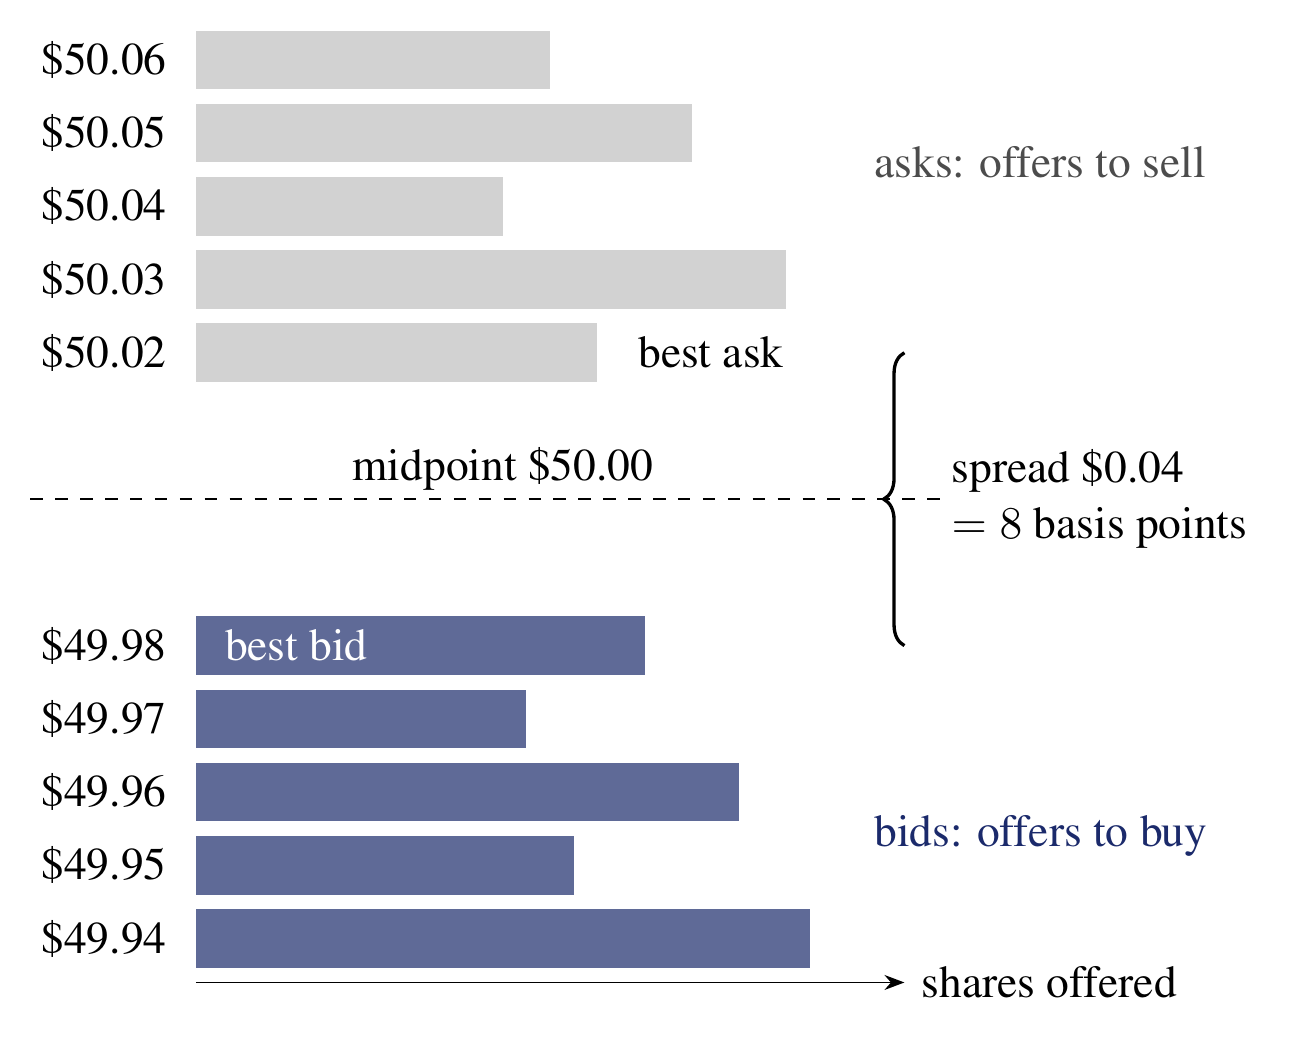
\includegraphics[width=0.8\linewidth]{images/fig06-1-order-book.png}
%\caption{A limit order book. Sellers' asks sit above the midpoint and buyers' bids below it. A buyer who wants to trade at once pays the best ask, \$50.02; a seller receives the best bid, \$49.98. The gap of \$0.04, 8 basis points of the \$50.00 midpoint, is the bid--ask spread.}
%\label{fig:06-book}
%\end{figure}

\textbf{Market and limit orders.} There are two basic ways to trade.

\begin{itemize}
  \item A \textbf{market order} trades immediately against the best available quotes: a buyer pays the ask, a seller receives the bid. Market orders \emph{demand} liquidity and pay the spread.
  \item A \textbf{limit order} sets a price and waits in the book until someone trades against it. Limit orders \emph{supply} liquidity and may earn the spread, but risk not being filled, or being filled just before the price moves against them.
\end{itemize}

Large orders are usually broken into many small ones and executed over hours or days to limit their effect on prices.

\textbf{Who provides liquidity.} \textbf{Market makers} and high-frequency traders post bids and asks continuously and earn the spread. In return they bear \textbf{inventory risk}, the risk that prices move while they hold shares they have bought but not yet sold, and the risk of trading with better-informed investors. Spreads are wider for small, volatile and thinly traded stocks because these risks are larger there.

\textbf{Long and short positions.} A \textbf{long} position owns a security and gains when its price rises. A \textbf{short} position borrows shares, sells them, and must later buy them back to return them; it gains when the price falls. The short seller pays any dividends to the lender, posts \textbf{collateral} (cash or securities held as security for the loan), and pays a \textbf{borrowing fee} set in the securities-lending market. Most large stocks are cheap to borrow; a minority are hard to borrow and expensive, and the lender can \textbf{recall} the loan, forcing the short seller to buy the shares back.

\textbf{Long--short portfolios.} Academic factors such as HML are \textbf{zero-investment} portfolios: one dollar long, one dollar short, so the proceeds of the short sale pay for the long side. Their returns are the difference between the two sides, so a factor's ``return'' is a spread, not the return on capital invested. In practice a long--short fund must hold collateral and capital against both sides, and returns are quoted relative to that capital.

\textbf{Turnover.} \textbf{Turnover} measures how much of a portfolio is traded in a period. One-sided monthly turnover of 10\% means a tenth of the portfolio is sold, and replaced, each month. Turnover multiplies every per-trade cost: a strategy that replaces its whole portfolio monthly pays its trading costs twelve times a year on each side.

\textbf{Worked example.} A stock is quoted at \$49.98 bid and \$50.02 ask. The midpoint is \$50.00 and the spread is \$0.04, or $0.04/50 = 0.0008$, 8 basis points. Buying with a market order and immediately selling would lose 8 basis points; the one-way cost, half the spread, is 4 basis points.

\textbf{Further reading.} Harris, \emph{Trading and Exchanges: Market Microstructure for Practitioners}, the standard introduction; Bodie, Kane and Marcus, \emph{Investments}, chapters on how securities are traded, including short sales and margin; Hull, \emph{Options, Futures, and Other Derivatives}, introductory chapters on the mechanics of short selling and margin accounts.

\section{Paper returns versus implementable returns}
\label{sec:06-paper}

The factor returns in the Kenneth French Data Library, like most portfolio returns in academic research, are \textbf{paper returns}. Each month the portfolio is rebuilt from the latest sorts, at closing prices, with no charge for trading. The construction is deliberately simple and transparent, which is why the data is so useful. But it answers the question ``what pattern exists in returns?'' rather than ``what could an investor have earned?''

An \textbf{implementable return}, one an investor could actually have earned, differs in four ways:

\begin{enumerate}
  \item \textbf{Trading costs.} Every purchase pays above the midpoint price and every sale receives below it; large orders also move the price.
  \item \textbf{Short-selling costs and limits.} Selling short requires borrowing shares, which costs a fee, may be impossible for some stocks, and can be recalled.
  \item \textbf{Timing and execution.} Signals computed from closing prices cannot be traded at those same prices. Orders take time to work, and fast-moving signals lose value while they wait.
  \item \textbf{Scale.} A strategy that works with \$10 million may not work with \$10 billion, because the trades themselves change prices.
\end{enumerate}

None of these makes a paper return wrong. A pattern that cannot be traded profitably may still tell us something about risk or about how prices form. But a claim about profits needs an implementable return, and the two can differ by more than the whole premium.

The gap is largest for strategies that trade often, in small or illiquid stocks, or on the short side. It is smallest for slow strategies in large stocks, which is one reason the market portfolio itself is so hard to beat after costs: it barely trades at all.

\section{The anatomy of trading costs}
\label{sec:06-anatomy}

The cost of a trade has several parts, and they behave differently.

\begin{center}
\small
\begin{tabularx}{0.9\linewidth}{@{}>{\raggedright\arraybackslash}p{0.19\linewidth}>{\raggedright\arraybackslash}X>{\raggedright\arraybackslash}p{0.32\linewidth}@{}}
\toprule
Component & What it is & How it scales \\
\midrule
Commissions and fees & Payments to brokers and exchanges & Small for institutions today; roughly proportional to the amount traded \\
Bid--ask spread & Buying at the ask and selling at the bid, above and below the midpoint & Proportional to the amount traded; wider for small, volatile and illiquid stocks \\
Market impact & The price moving against an order while it is executed, because the order itself carries information or demands liquidity & Grows faster than the trade: roughly with the square root of the order's size relative to volume \\
Delay and opportunity cost & Prices moving before the order is filled, or trades not made at all & Largest for fast signals \\
Short-selling costs & Fees to borrow shares, the risk of recall, rules that restrict shorting & Mostly small, very large for a minority of stocks \\
\bottomrule
\end{tabularx}
\end{center}

The unit used throughout this chapter is the \textbf{one-way cost}: the cost of buying, or of selling, one dollar of stock, as a fraction of the dollar. For a small trade it is roughly half the bid--ask spread plus commissions. A \textbf{round trip}, buying and later selling, costs twice the one-way cost.

\textbf{Costs have fallen, unevenly.} U.S. equity spreads narrowed sharply after prices moved from fractions to decimals in 2001, a change called \textbf{decimalization}, and as electronic trading spread. Large-cap stocks now trade at spreads of a few basis points; small, illiquid stocks still cost far more. This matters for interpreting long histories: a strategy tested from 1963 faced costs in its early decades that were several times today's, so applying today's costs to the whole history flatters the past, and applying the past's costs to today understates what is possible now.

\textbf{Short selling.} A short seller borrows shares and pays a lending fee. D'Avolio (2002) found that the large majority of U.S. stocks were cheap to borrow, but that a small set of ``special'' stocks carried high fees, and that these were often exactly the stocks with the strongest short signals. Borrowing can also be recalled at inconvenient times, and regulators can ban shorting outright, as the U.S. Securities and Exchange Commission did for financial stocks in September 2008. Miller (1977) argued that when pessimists cannot short, prices reflect only the optimists' views, so overpricing can persist; Stambaugh, Yu and Yuan (2012) found that many anomalies earn most of their profits on the short side, where these frictions bite. A long--short paper portfolio that ignores them overstates what is achievable, sometimes by most of the premium.

The lab uses a single one-way cost and a single borrowing fee for transparency. Real costs vary across stocks and over time, and Section~\ref{sec:06-measuring} shows how they can be estimated.

\section{Measuring costs from public data}
\label{sec:06-measuring}

The best measure of trading costs is a trader's own record. \textbf{Implementation shortfall} (Perold 1988) compares the value of a paper portfolio at the prices when the decision was made with the value of the portfolio actually achieved, capturing spreads, impact, delay and trades never completed. Most researchers do not have such records, so the field relies on estimates.

\textbf{From quotes and trades.} With intraday data, such as the TAQ (Trade and Quote) database of every U.S. trade and quote, two spreads can be measured:

\begin{itemize}
  \item the \textbf{quoted spread}, the gap between the best bid and ask;
  \item the \textbf{effective spread}, twice the difference between the trade price and the midpoint at the time of the trade.
\end{itemize}

Effective spreads are usually smaller than quoted ones, because many trades execute inside the quotes.

\textbf{From daily data.} Several estimators infer spreads from daily prices alone, which makes them available back to the 1920s:

\begin{itemize}
  \item \textbf{Roll (1984)} infers the spread from \textbf{bid--ask bounce}: because trades alternate randomly between the bid and the ask, successive price changes are negatively correlated, and the size of that correlation reveals the spread.
  \item \textbf{Hasbrouck (2009)} estimates a similar model with a Bayesian Gibbs sampler, a simulation-based estimation method, which is more robust when the Roll estimator fails.
  \item \textbf{Corwin and Schultz (2012)} use daily high and low prices: highs are usually trades at the ask and lows at the bid, and the spread's share of the range can be separated from volatility by comparing one-day and two-day ranges.
  \item \textbf{Abdi and Ranaldo (2017)} combine closing, high and low prices for a more precise estimator.
  \item \textbf{Amihud (2002)} measures \textbf{illiquidity} as the average absolute return per dollar of volume: a measure of price impact rather than a spread.
\end{itemize}

These estimators are noisy for any one stock and month, but useful averaged across portfolios, which is how Novy-Marx and Velikov (2016) used them to estimate the costs of dozens of anomalies.

\textbf{Estimates from practice.} Frazzini, Israel and Moskowitz (2018) studied \$1.7 trillion of actual trades by a large institutional manager across 21 developed markets over 19 years, and found trading costs an order of magnitude smaller than earlier academic estimates suggested. Their result is a reminder that costs depend on who is trading and how: a patient institution that provides liquidity pays far less than the generic investor assumed by spread estimators. It is also a reminder that the evidence comes from one manager's experience, under that manager's trading methods.

The practical consequence is that a cost assumption is a judgment. A careful study reports results across a range of costs, and the lab does so, from zero to 100 basis points one way.

\section{Turnover, net returns and break-even costs}
\label{sec:06-turnover}

\textbf{Turnover} measures how much a portfolio trades. One-sided monthly turnover is the share of the portfolio sold, and replaced, each month: half the sum of the absolute changes in portfolio weights, measured against the weights the portfolio would have drifted to with no trading. A value-weighted portfolio whose membership never changes has zero turnover, however much its prices move.

What drives turnover is how fast the signal changes relative to how often the portfolio is rebuilt:

\begin{itemize}
  \item \textbf{Value} sorts on book-to-market once a year. Book-to-market ratios are persistent, so most stocks stay on the same side from one year to the next.
  \item \textbf{Momentum} sorts monthly on the return from 12 months to 2 months ago. Each month's window shares ten of its eleven months with the last one, but enough stocks cross the \textbf{breakpoints}, the cut-offs between groups, to replace about a third of the portfolio each month.
  \item \textbf{Short-term reversal} sorts monthly on the previous month's return, which has almost no persistence. Nearly the whole portfolio is replaced every month.
\end{itemize}

\textbf{From gross to net.} A \textbf{gross} return is before costs; a \textbf{net} return is after them. A long--short portfolio with one dollar on each side and one-sided turnover $T$ sells and buys $T$ on each side, so it trades $4T$ dollars a month. At a one-way cost $c$, its monthly cost and net return are
\begin{equation}
  \text{cost} = 4\,T\,c, \qquad r^{net}_t = r^{gross}_t - 4\,T\,c - \frac{\text{borrow fee}}{12}
  \label{eq:06-net}
\end{equation}

The \textbf{break-even cost} is the one-way cost at which the average net return is zero:
\begin{equation}
  c^* = \frac{\text{average gross return} - \text{other costs}}{4T}
  \label{eq:06-breakeven}
\end{equation}
It answers the most useful question about a strategy's costs: how cheaply must it trade to be worth trading? For example, a strategy with turnover of 10\% a month that earns 0.4\% a month gross can pay up to $0.4/(4 \times 0.10) = 1\%$ per trade before its profit is gone.

Novy-Marx and Velikov (2016) estimated turnover and costs for value-weighted versions of many anomalies. Their full-sample figures for the three strategies in this chapter (Table 3 of the working-paper version), with break-even costs computed from their gross returns using Equation~\eqref{eq:06-breakeven}:

\begin{center}
\small
\begin{tabularx}{0.9\linewidth}{@{}>{\raggedright\arraybackslash}X>{\raggedright\arraybackslash}p{0.13\linewidth}>{\raggedright\arraybackslash}p{0.13\linewidth}>{\raggedright\arraybackslash}p{0.13\linewidth}>{\raggedright\arraybackslash}p{0.13\linewidth}>{\raggedright\arraybackslash}p{0.12\linewidth}@{}}
\toprule
Strategy & One-sided monthly turnover & Gross return (\% per month) & Estimated cost (\% per month) & Net return (\% per month) & Break-even one-way cost \\
\midrule
Value (book-to-market) & 2.9\% & 0.47 & 0.05 & 0.42 & about 4\% \\
Momentum & 34.5\% & 1.33 & 0.65 & 0.68 & about 1\% \\
Short-term reversal & 90.9\% & 0.37 & 1.65 & $-1.28$ & about 0.1\% \\
\bottomrule
\end{tabularx}
\end{center}

The three strategies sit on very different sides of realistic costs (Figure~\ref{fig:06-breakeven}). Value could pay several percent per trade and still profit. Momentum survives costs of up to roughly one percent per trade, which a careful institution can achieve but a careless one may not. Short-term reversal, profitable on paper, would need to trade for about ten basis points per trade, below what most investors pay for the small, recently volatile stocks it buys and sells. Its paper profit is real, but tiny relative to the trading it requires.


\providecolor{fenavy}{HTML}{1B2A6B}

\begin{figure}[htbp]
  \centering
  \begin{tikzpicture}[
    % Gross return (% a month) and monthly one-way turnover, from the table.
    % Net return = gross - 4 * turnover * cost; break-even = gross / (4 * turnover).
    declare function={
      valG = 0.47;  valT = 0.029;
      momG = 1.33;  momT = 0.346;
      revG = 0.38;  revT = 0.95;
    }]
  \begin{axis}[
    width=0.82\linewidth, height=0.5\linewidth,
    axis lines=left,
    axis line style={-stealth, thin},
    xmin=0, xmax=1.3, ymin=-1.6, ymax=1.45,
    xtick={0,0.2,0.4,0.6,0.8,1,1.2},
    ytick={-1,0,1},
    xticklabel style={/pgf/number format/fixed},
    xlabel={One-way trading cost (\%)},
    ylabel={Net return (\% a month)},
    clip=false,
  ]
    \addplot[gray!60, thin, domain=0:1.3, samples=2] {0};

    % Value
    \addplot[fenavy, very thick, domain=0:1.3, samples=2] {valG - 4*valT*x};
    % Momentum
    \addplot[thick, dashed, domain=0:1.3, samples=2] {momG - 4*momT*x};
    % Short-term reversal (stops at the bottom of the chart)
    \addplot[very thick, densely dotted, domain=0:0.52, samples=2] {revG - 4*revT*x};

    % Break-even points
    \fill (axis cs:{momG/(4*momT)},0) circle (2.2pt);
    \fill (axis cs:{revG/(4*revT)},0) circle (2.2pt);
    \node[anchor=north east, font=\small] at (axis cs:{momG/(4*momT)-0.02},-0.03)
      {break-even $\approx 1\%$};
    \node[anchor=south west, font=\small] at (axis cs:{revG/(4*revT)+0.03},0.03)
      {$\approx 0.1\%$};

    % Line labels
    \node[fenavy, anchor=west, font=\small] at (axis cs:1.31,{valG-4*valT*1.3+0.05}) {value};
    \node[anchor=west, font=\small] at (axis cs:1.31,{momG-4*momT*1.3}) {momentum};
    \node[anchor=west, font=\small] at (axis cs:0.48,-1.05) {short-term reversal};
  \end{axis}
  \end{tikzpicture}
  \caption{Net return against one-way trading cost, from the turnover and gross
    returns in the table. Each line falls at a rate of four times the strategy's
    turnover; it crosses zero at the break-even cost. Value's line is nearly
    flat and crosses zero off the chart, at about 4\%.}
  \label{fig:06-breakeven}
\end{figure}

%\begin{figure}[htbp]
%\centering
%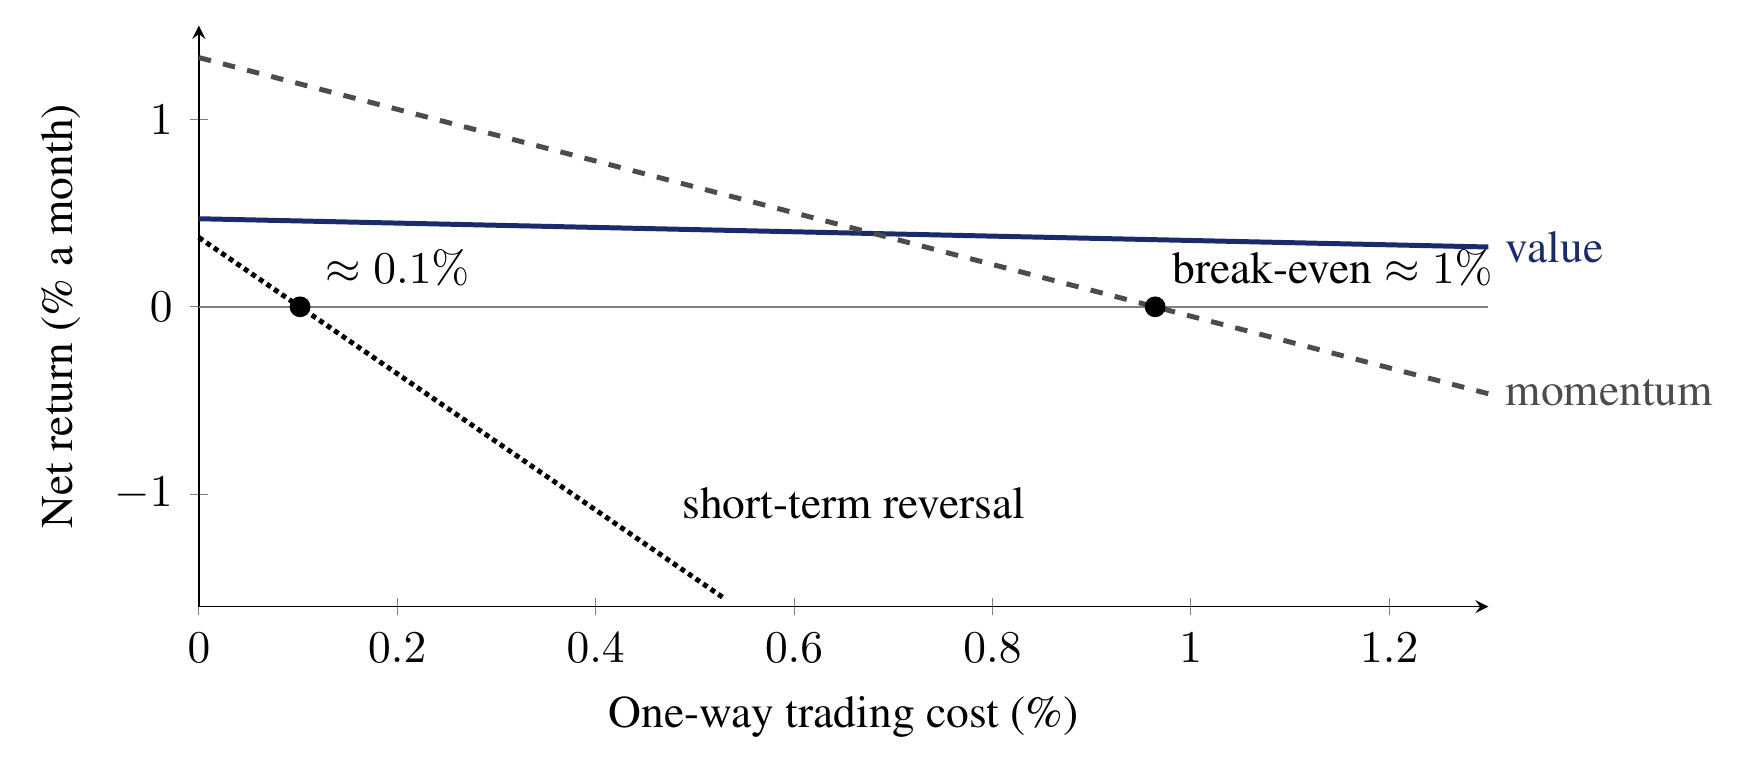
\includegraphics[width=0.85\linewidth]{images/fig06-2-break-even.png}
%\caption{Net return against one-way trading cost, from the turnover and gross returns in the table. Each line falls at a rate of four times the strategy's turnover; it crosses zero at the break-even cost. Value's line is nearly flat and crosses zero off the chart, at about 4\%.}
%\label{fig:06-breakeven}
%\end{figure}

A gross ranking by Sharpe ratio or t-statistic therefore says little about which strategy an investor should prefer. The net ranking depends on turnover as much as on the gross premium.

\section{Market impact and capacity}
\label{sec:06-capacity}

Spreads are roughly a fixed cost per dollar traded. Market impact is not: the more a strategy trades relative to the market's volume, the more each dollar costs. This is what gives every strategy a \textbf{capacity}, a size beyond which its net returns shrink toward zero.

\textbf{Why prices move.} Kyle (1985) modeled market makers who cannot tell informed orders from uninformed ones and so move prices in the direction of every order. Large orders, which are more likely to be informed and more costly to absorb, move prices more. Empirical studies of institutional executions find that impact grows roughly with the square root of an order's size relative to daily volume (Almgren, Thum, Hauptmann and Li 2005; T\'oth et al.\ 2011). A common working model is
\begin{equation}
  \text{impact per dollar} \approx Y\,\sigma_{daily}\,\sqrt{\frac{Q}{V}}
  \label{eq:06-impact}
\end{equation}
where $Q$ is the order size, $V$ is daily volume, $\sigma_{daily}$ is daily volatility and $Y$ is a constant of order one. The ratio $Q/V$ is the \textbf{participation rate}, the order's share of the day's trading. Trading 1\% of a day's volume in a stock with 2\% daily volatility costs about $2\% \times \sqrt{0.01} = 0.2\%$ in impact; trading 10\% costs about $2\% \times \sqrt{0.10} \approx 0.6\%$ (Figure~\ref{fig:06-impact}).


\providecolor{fenavy}{HTML}{1B2A6B}

\begin{figure}[htbp]
  \centering
  \begin{tikzpicture}[
    % Impact (%) = Y * sigma * sqrt(Q/V), with Y = 1 and sigma = 2%.
    % x is Q/V in percent, so impact = 2 * sqrt(x/100) = 0.2 * sqrt(x).
    declare function={impact(\x) = 0.2*sqrt(\x);}
  ]
  \begin{axis}[
    width=0.74\linewidth, height=0.47\linewidth,
    axis lines=left,
    axis line style={-stealth, thin},
    xmin=0, xmax=20.5, ymin=0, ymax=1,
    xtick={0,2,...,20},
    ytick={0,0.2,0.4,0.6,0.8,1},
    yticklabel style={/pgf/number format/fixed},
    tick label style={font=\small},
    xlabel={Order size as a share of daily volume, $Q/V$ (\%)},
    ylabel={Impact per dollar traded (\%)},
    samples=200, domain=0:20,
    clip=false,
  ]
    % If impact were linear (for comparison)
    \addplot[gray!70, densely dashed, thin, samples=2] {0.0215*x};
    \node[gray!40!black, font=\small, anchor=west] at (axis cs:20.2,0.43)
      {if impact were linear};

    % Square-root impact
    \addplot[fenavy, very thick] {impact(x)};
    \node[fenavy, font=\small, anchor=west] at (axis cs:20.2,{impact(20)})
      {square root};

    % Marked points
    \fill[fenavy] (axis cs:1,0.2) circle (2.2pt);
    \draw[gray!50] (axis cs:1.2,0.21) -- (axis cs:4.6,0.34);
    \node[font=\small, anchor=west] at (axis cs:4.6,0.34) {1\% of volume: 0.2\%};

    \fill[fenavy] (axis cs:10,0.632) circle (2.2pt);
    \node[font=\small, anchor=north west] at (axis cs:10.3,0.6)
      {10\% of volume: 0.6\%};
  \end{axis}
  \end{tikzpicture}
  \caption{Square-root market impact for a stock with 2\% daily volatility,
    from Equation~\eqref{eq:06-impact} with $Y = 1$. Ten times the order size
    costs about three times as much per dollar, not ten times; but total
    impact cost, per dollar times dollars, still rises faster than the order.}
  \label{fig:06-impact}
\end{figure}

%\begin{figure}[htbp]
%\centering
%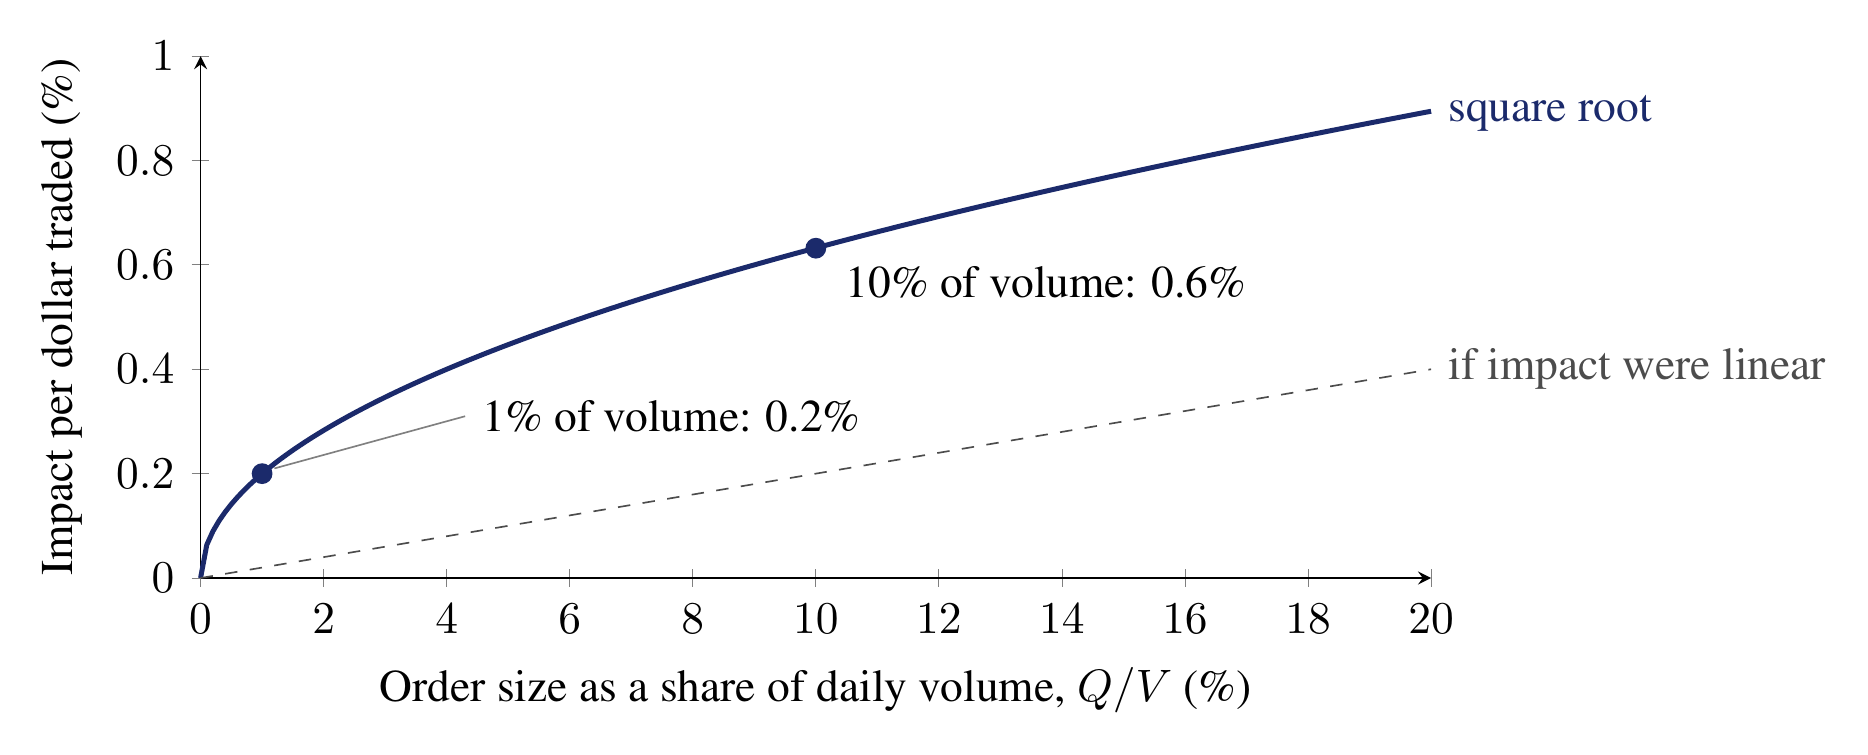
\includegraphics[width=0.85\linewidth]{images/fig06-3-impact.png}
%\caption{Square-root market impact for a stock with 2\% daily volatility, from Equation~\eqref{eq:06-impact} with $Y = 1$. Ten times the order size costs about three times as much per dollar, not ten times; but total impact cost, per dollar times dollars, still rises faster than the order.}
%\label{fig:06-impact}
%\end{figure}

\textbf{From impact to capacity.} A strategy managing assets $A$ with turnover $T$ trades about $2TA$ on each side every month, spread across its holdings. As $A$ grows, the participation rate $Q/V$ rises, impact per dollar rises with its square root, and total impact cost rises faster than the assets. Net return therefore falls with size, slowly at first and then quickly. Capacity can be defined as the size at which the net return is halved, or reaches zero; an investor would want to stop well before either.

Three features of a strategy set its capacity:

\begin{enumerate}
  \item \textbf{Turnover.} Every dollar not traded is a dollar that does not move prices.
  \item \textbf{Liquidity of its holdings.} Strategies that concentrate in small stocks hit their limits first.
  \item \textbf{Gross premium.} A larger premium can absorb more cost before it is gone.
\end{enumerate}

Capacity also has an industry-wide side. If many managers follow similar signals, their combined trades determine impact, and a strategy's capacity is shared among everyone trading it. Berk and Green (2004) argued that in a competitive market, money flows into skilled managers until their returns after costs are no better than the alternative, a theme Chapter 24 returns to.

The capacity estimates in this chapter's lab rest on stated assumptions about volume, spreads and the impact constant. They are an illustration of how capacity arises and what it depends on, not a forecast for any real fund.

\section{Designing for costs}
\label{sec:06-design}

A paper portfolio is built as if trading were free, so it trades whenever the signal moves, however slightly. A portfolio designed for costs trades only when the expected gain exceeds the cost. Several simple rules capture most of the benefit.

\begin{itemize}
  \item \textbf{Buy/hold spreads (banding).} Buy a stock only when it enters the top 30\% on the signal, but keep holding it until it falls out of, say, the top 50\%. Stocks that wobble around the breakpoint no longer generate trades. Novy-Marx and Velikov (2016) found this the single most effective simple way to reduce costs.
  \item \textbf{Slower rebalancing.} Rebuilding the portfolio quarterly rather than monthly cuts turnover for slow signals at little cost in signal. For fast signals it gives up most of the premium.
  \item \textbf{Partial trading.} G\^arleanu and Pedersen (2013) showed that with predictable returns and \textbf{quadratic trading costs}, costs that rise with the square of the amount traded, the optimal policy trades only part of the way toward the target each period, and aims at a target that anticipates where the signal is heading.
  \item \textbf{Netting and combining signals.} A multi-signal portfolio can cross trades internally: a stock that momentum wants to sell and value wants to buy need not be traded at all.
  \item \textbf{Liquidity screens.} Restricting the universe to larger, more liquid stocks raises capacity and lowers costs, usually at some cost in gross premium, since many anomalies are strongest in small stocks.
\end{itemize}

Each rule trades a little signal for a lot less trading. The trade-off depends on how fast the signal decays: banding costs little for momentum, whose ranks change gradually, and cannot rescue short-term reversal, whose signal is gone within a month.

\textbf{Cost mitigation is also a search.} Every design choice, a band width, a rebalancing frequency, a liquidity screen, can be tuned to make a backtest look better, and Chapter 4's warnings apply in full. Chen and Velikov (2023) examined 204 anomalies, accounting for effective spreads, post-publication decay and the modern era of trading technology, and found that the average anomaly's expected return net of these effects was about 4 basis points a month. Strategies with impressive net returns in-sample, after cost mitigation, did not escape that conclusion. A cost-aware design should be specified in advance, and judged out of sample like any other part of the strategy.

\begin{callout}
\textbf{What Failed: buying last month's losers.} Jegadeesh (1990) and Lehmann (1990) documented that stocks with low returns over the past week or month tended to rebound, and stocks with high returns to fall back. The pattern is strong and statistically robust on paper, and the Fama--French short-term reversal factor still records a positive average return. But the strategy replaces almost its whole portfolio every month, concentrating in stocks that have just moved sharply, often small and illiquid ones, exactly where spreads are widest. Novy-Marx and Velikov (2016) estimated that its costs exceeded its gross return by more than a percentage point a month. Much of the reversal itself may be compensation for providing liquidity to impatient traders (Nagel 2012), a return that accrues to market makers who face low costs, not to investors who must pay the spread. As a strategy for an ordinary investor, the claim that buying recent losers is profitable \textbf{fails} once costs are counted.
\end{callout}

\section{Lab 6: What survives the trip from paper to portfolio?}
\label{sec:06-lab}

\begin{callout}
\textbf{Lab 6 at a glance.} \emph{Claim on trial:} a strategy that is profitable in a backtest is profitable to trade. \emph{Data:} three long--short factors from the Kenneth R. French Data Library, value (HML), momentum (Mom) and short-term reversal (ST Rev), from July 1963, plus a simulated stock universe. \emph{Run time:} a few seconds. \emph{Code:} repository folder \texttt{ch06-costs/}, with a guided notebook.
\end{callout}

The lab takes the three factors and asks what each would have earned after costs.

\textbf{Part A: gross performance.} Average returns, t-statistics and Sharpe ratios as published. On paper, all three look like discoveries.

\textbf{Part B: turnover.} The French library does not publish holdings, so turnover comes from two sources. The first is Novy-Marx and Velikov's estimates for value-weighted versions of the same strategies. The second is a simulated stock universe of 1,000 stocks over 40 years, with fat-tailed returns, a realistic spread of company sizes, and portfolios built exactly as the Fama--French factors are: value-weighted 30/70 sorts, value updated each June, momentum and reversal each month. Because the simulated universe has no delistings or new listings, its turnover is a lower bound. In the version shipped with the lab it gives about 2\% a month for value, 25\% for momentum and 76\% for reversal, the same ordering and similar magnitudes as the published estimates, which shows that turnover follows mechanically from how each signal is built.

\textbf{Part C: costs.} Net returns across one-way costs from 0 to 100 basis points, plus a short-borrowing fee of 0.25\% a year; break-even costs; and the ranking of the three strategies by Sharpe ratio before and after costs at a headline cost of 20 basis points. Figure 6.4 plots each strategy's net return against cost, with its break-even point marked; Figure 6.5 shows the growth of a dollar on paper and after costs.

\textbf{Part D: capacity.} The simulated universe is scaled to a \$50 trillion market, with daily volume of 0.4\% of each company's value, half-spreads from 2 basis points for the largest stocks to 50 for the smallest, and square-root impact. Each strategy's net return is traced as its assets grow from \$10 million to \$1 trillion. The assumptions are explicit and adjustable, and the exercises ask which matters most.

\textbf{Part E: mitigation, with known truth.} In the simulated universe, expected returns are known, so cost-mitigation rules can be compared without sampling noise. The lab compares the standard sort with buy/hold spreads of increasing width. For momentum at a one-way cost of 50 basis points, holding stocks until they leave the top 50\% cuts turnover roughly in half, from about 25\% to 12\% a month, gives up about a fifth of the expected gross return, and raises the expected net return from about 0.30\% to 0.41\% a month. For reversal, no band width rescues the strategy at that cost: the signal decays too fast for patience to pay.

The lab, its tests and a guided notebook are in \texttt{ch06-costs} in the book's repository. The README records what has been tested and how, including that the parsers for the momentum and reversal files have been tested on the library's layout but not yet on the live files.

\section{What investors can use}
\label{sec:06-investors}

The verdict on the claim: \textbf{fails} as a general rule. Whether a profitable backtest is profitable to trade depends on how much it trades, what it trades, and how much money is behind it. Slow strategies in liquid stocks survive realistic costs comfortably; fast strategies in small stocks often do not survive them at all. The claim holds only for strategies whose break-even costs sit well above what their investors actually pay, at the size they intend to run.

Five questions turn the chapter into a checklist for any strategy an investor is shown:

\begin{enumerate}
  \item \textbf{What is the turnover?} Ask for one-sided monthly turnover, on both sides. If the answer is not known, the strategy has not been evaluated as an investment.
  \item \textbf{What is the break-even cost, and what will you pay?} Compare the break-even one-way cost with realistic costs for the stocks the strategy holds, in the period it will be traded. A strategy that needs costs below ten basis points is a bet on execution, not on the signal.
  \item \textbf{What does the short side cost?} Ask how much of the return comes from the short side, what borrowing fees were assumed, and how the strategy would behave if hard-to-borrow stocks could not be shorted.
  \item \textbf{At what size?} Ask for net returns at the assets the manager plans to run, and how the estimate of market impact was made. Capacity claims without stated assumptions are marketing.
  \item \textbf{Were cost-saving rules chosen in advance?} Bands, rebalancing schedules and liquidity screens are sensible, but each is a parameter. Ask whether they were fixed before the backtest, and how the strategy performed after they were.
\end{enumerate}

The broader lesson is that costs change the ranking of strategies, not just their level. A modest, slow premium that can be harvested cheaply may be worth more than a spectacular, fast one that cannot. Chapters 8 to 10 test the best-known anomalies; every verdict there is reported after costs as well as before.

\section*{Exercises}
\addcontentsline{toc}{section}{Exercises}

\subsection*{Conceptual (all readers)}

\begin{enumerate}
  \item A long--short strategy has one-sided monthly turnover of 20\% and earns 0.6\% a month gross. What is its break-even one-way cost? What is its net return at a one-way cost of 30 basis points?
  \item Explain why a value-weighted portfolio whose membership never changes has zero turnover, while an equal-weighted one with the same membership does not.
  \item Why does market impact give a strategy a capacity, while a fixed spread does not?
  \item A strategy earns most of its paper return on the short side. List three reasons its implementable return could be much lower than its paper return.
\end{enumerate}

\subsection*{Lab extensions (technical readers)}

\begin{enumerate}
  \setcounter{enumi}{4}
  \item Re-run the lab from May 2001, after the move to decimal prices, with a one-way cost of 10 basis points. Does short-term reversal survive in the low-cost era?
  \item Re-run Part C with a borrowing fee of 2\% a year. Which strategy is most exposed to shorting costs, and why?
  \item In Part D, halve and double the impact constant and the number of days over which trades are spread. Which assumption moves capacity most? What evidence would you want before trusting it?
  \item In Part E, add a rule that rebalances momentum only once a quarter. Compare its turnover and expected net return with banding.
  \item Implement the Corwin--Schultz high--low spread estimator and apply it to daily data for a few stocks you can download. How does it compare with their quoted spreads?
  \item Choose an anomaly from Chapter 10's list. Estimate its turnover from its construction, compute its break-even cost, and judge whether it is likely to survive costs.
\end{enumerate}

\section*{References}
\addcontentsline{toc}{section}{References}

\begin{itemize}
  \item Abdi, F. and Ranaldo, A. (2017). A Simple Estimation of Bid-Ask Spreads from Daily Close, High, and Low Prices. \emph{Review of Financial Studies} 30(12): 4437--4480.
  \item Almgren, R., Thum, C., Hauptmann, E. and Li, H. (2005). Direct Estimation of Equity Market Impact. \emph{Risk} 18(7): 58--62.
  \item Amihud, Y. (2002). Illiquidity and Stock Returns: Cross-Section and Time-Series Effects. \emph{Journal of Financial Markets} 5(1): 31--56.
  \item Berk, J. B. and Green, R. C. (2004). Mutual Fund Flows and Performance in Rational Markets. \emph{Journal of Political Economy} 112(6): 1269--1295.
  \item Chen, A. Y. and Velikov, M. (2023). Zeroing In on the Expected Returns of Anomalies. \emph{Journal of Financial and Quantitative Analysis} 58(3): 968--1004.
  \item Corwin, S. A. and Schultz, P. (2012). A Simple Way to Estimate Bid-Ask Spreads from Daily High and Low Prices. \emph{Journal of Finance} 67(2): 719--760.
  \item D'Avolio, G. (2002). The Market for Borrowing Stock. \emph{Journal of Financial Economics} 66(2--3): 271--306.
  \item Frazzini, A., Israel, R. and Moskowitz, T. J. (2018). Trading Costs. Working paper, SSRN 3229719.
  \item G\^arleanu, N. and Pedersen, L. H. (2013). Dynamic Trading with Predictable Returns and Transaction Costs. \emph{Journal of Finance} 68(6): 2309--2340.
  \item Hasbrouck, J. (2009). Trading Costs and Returns for U.S. Equities: Estimating Effective Costs from Daily Data. \emph{Journal of Finance} 64(3): 1445--1477.
  \item Jegadeesh, N. (1990). Evidence of Predictable Behavior of Security Returns. \emph{Journal of Finance} 45(3): 881--898.
  \item Kyle, A. S. (1985). Continuous Auctions and Insider Trading. \emph{Econometrica} 53(6): 1315--1335.
  \item Lehmann, B. N. (1990). Fads, Martingales, and Market Efficiency. \emph{Quarterly Journal of Economics} 105(1): 1--28.
  \item Miller, E. M. (1977). Risk, Uncertainty, and Divergence of Opinion. \emph{Journal of Finance} 32(4): 1151--1168.
  \item Nagel, S. (2012). Evaporating Liquidity. \emph{Review of Financial Studies} 25(7): 2005--2039.
  \item Novy-Marx, R. and Velikov, M. (2016). A Taxonomy of Anomalies and Their Trading Costs. \emph{Review of Financial Studies} 29(1): 104--147. Working-paper version: NBER Working Paper 20721.
  \item Perold, A. F. (1988). The Implementation Shortfall: Paper versus Reality. \emph{Journal of Portfolio Management} 14(3): 4--9.
  \item Roll, R. (1984). A Simple Implicit Measure of the Effective Bid-Ask Spread in an Efficient Market. \emph{Journal of Finance} 39(4): 1127--1139.
  \item Stambaugh, R. F., Yu, J. and Yuan, Y. (2012). The Short of It: Investor Sentiment and Anomalies. \emph{Journal of Financial Economics} 104(2): 288--302.
  \item T\'oth, B., Lemp\'eri\`ere, Y., Deremble, C., de Lataillade, J., Kockelkoren, J. and Bouchaud, J.-P. (2011). Anomalous Price Impact and the Critical Nature of Liquidity in Financial Markets. \emph{Physical Review X} 1(2): 021006.
\end{itemize}

\textbf{Data:} Kenneth R. French Data Library: Fama/French 3 Factors; Momentum Factor (Mom); Short-Term Reversal Factor (ST Rev), monthly. \url{https://mba.tuck.dartmouth.edu/pages/faculty/ken.french/data_library.html}

% Chapter 7 -- Claim: Stock Returns Are Predictable
% Requires: amsmath, amssymb, booktabs, array, tabularx, graphicx, tcolorbox (breakable, skins), hyperref or url.
% Defines the callout box only if the preamble has not.
\providecolor{fenavy}{HTML}{1B2A6B}
\providecolor{feshade}{HTML}{F3F5FA}
\makeatletter
\@ifundefined{callout}{%
  \newtcolorbox{callout}{breakable, enhanced,
    colback=white, colframe=gray!70, boxrule=0.5pt, arc=1mm,
    borderline west={2.5pt}{0pt}{gray!70},
    left=8pt, right=8pt, top=4pt, bottom=4pt}%
}{}
\makeatother

\chapter{Claim: Stock Returns Are Predictable}
\label{ch:07}

This is the first of the book's claim chapters. Chapters 1 to 6 built the tools: statistics for noisy returns, corrections for searching, honest out-of-sample tests and trading costs. From here on, each chapter takes one widely held claim and puts it on trial with those tools, following the same steps: how the idea works, the claim stated so it can fail, the evidence that made it famous, a replication on open data, stress tests, and a dated verdict.

The first claim is one of the oldest and most consequential in finance. If stock returns are predictable from valuations, then investors can time the market, retirement plans should assume lower returns when prices are high, and the efficient-markets view that dominated the 1970s needs rethinking. Few empirical questions have been argued over longer, by more distinguished economists, with more at stake for ordinary savers.

The chapter's answer depends on what ``predictable'' is supposed to mean. For deciding whether to be in or out of stocks next month or next year, the evidence is weak. For setting a realistic range for the next decade's returns, valuations carry real information, though the range is wide. The lab lets you see both conclusions emerge from the same data.

By the end of the chapter you will be able to:

\begin{itemize}
  \item compute present values and use the Gordon growth model to link a dividend yield to expected returns and growth;
  \item distinguish expected from realized returns, and real from nominal returns;
  \item read a yield curve and compute a term spread;
  \item explain what valuation ratios such as the dividend--price ratio and CAPE measure, and why the Campbell--Shiller identity says they must carry information about the future;
  \item state the claim that returns are predictable in a form that can fail, and summarize the evidence for and against it;
  \item test the claim with corrected long-horizon regressions, a bootstrap for the Stambaugh bias and walk-forward forecasts;
  \item use valuations to set a range for long-run returns, rather than to time the market.
\end{itemize}

\section{Foundations: valuing a stock market, interest rates and inflation}
\label{sec:07-foundations}

\textbf{Present value.} A dollar received in the future is worth less than a dollar today, because today's dollar could be invested. The rate used to translate future money into today's money is the \textbf{discount rate}. At a discount rate $r$ per year, a cash flow $C$ received in $n$ years has a \textbf{present value} of $C/(1 + r)^n$: \$110 received in one year is worth \$100 today at a 10\% discount rate. The price of any asset can be written as the present value of the cash flows it is expected to pay, discounted at the return investors require to hold it.

\textbf{The dividend discount model.} Applied to a stock or a whole market, the cash flows are dividends. If dividends are expected to grow forever at a constant rate $g$, and investors require an expected return $r$ greater than $g$, the present value simplifies to the \textbf{Gordon growth model}:
\begin{equation}
  P_0 = \frac{D_1}{r - g} \qquad \Longleftrightarrow \qquad \frac{D_1}{P_0} = r - g
  \label{eq:07-gordon}
\end{equation}
where $P_0$ is today's price and $D_1$ next year's dividend. The second form is the key to this chapter: the \textbf{dividend yield} equals the required return minus expected growth. A high dividend yield must therefore mean either high required returns or low expected growth. The same logic applies to earnings: with a constant \textbf{payout ratio}, the share of earnings paid as dividends, the \textbf{earnings yield} $E/P$ (the inverse of the P/E ratio) is also tied to required returns and growth.

Because $r - g$ is small, the price is very sensitive to it (Figure~\ref{fig:07-gordon}). A one-point fall in the required return can raise the price by half. This is why stock markets can swing widely on changes in expected returns alone.

\providecolor{fenavy}{HTML}{1B2A6B}
\providecolor{feorange}{HTML}{B8481C}

\begin{figure}[htbp]
  \centering
  \begin{tikzpicture}[
    % Gordon growth model: P = D / (r - g), with D = $3 and g = 4%.
    % x is the required return in percent.
    declare function={price(\x) = 3/((\x - 4)/100);}
  ]
  \begin{axis}[
    width=0.8\linewidth, height=0.5\linewidth,
    axis lines=left,
    axis line style={-stealth, thin},
    xmin=5, xmax=10.3, ymin=0, ymax=230,
    xtick={5,6,7,8,9,10},
    xticklabels={5\%,6\%,7\%,8\%,9\%,10\%},
    ytick={0,50,100,150,200},
    yticklabels={\$0,\$50,\$100,\$150,\$200},
    tick label style={font=\small},
    xlabel={Required return, $r$},
    ylabel={Price, $P = D/(r - g)$},
    samples=200, domain=5.35:10,
    clip=false,
  ]
    \addplot[fenavy, very thick] {price(x)};

    % r = 7%: price $100, yield 3%
    \draw[gray, densely dashed, thin] (axis cs:7,0) -- (axis cs:7,100) -- (axis cs:5,100);
    \fill[fenavy] (axis cs:7,100) circle (2.2pt);
    \node[font=\small, anchor=south west, align=left] at (axis cs:7.1,102)
      {$r = 7\%$: price \$100,\\dividend yield 3\%};

    % r = 6%: price $150, yield 2%
    \draw[feorange, densely dashed, thin] (axis cs:6,0) -- (axis cs:6,150) -- (axis cs:5,150);
    \fill[feorange] (axis cs:6,150) circle (2.2pt);
    \node[feorange, font=\small, anchor=south west, align=left] at (axis cs:6.1,152)
      {$r = 6\%$: price \$150,\\dividend yield 2\%};

    \node[font=\small, anchor=north east, align=right, text=gray!40!black]
      at (axis cs:10.2,215) {$D = \$3$, $g = 4\%$};
  \end{axis}
  \end{tikzpicture}
  \caption{The Gordon growth model for a market paying a \$3 dividend next
    year, with dividends growing 4\% a year. Lowering the required return from
    7\% to 6\% raises the price from \$100 to \$150 and lowers the dividend
    yield from 3\% to 2\%. High prices and low yields go with low expected
    returns.}
  \label{fig:07-gordon}
\end{figure}

%\begin{figure}[htbp]
%\centering
%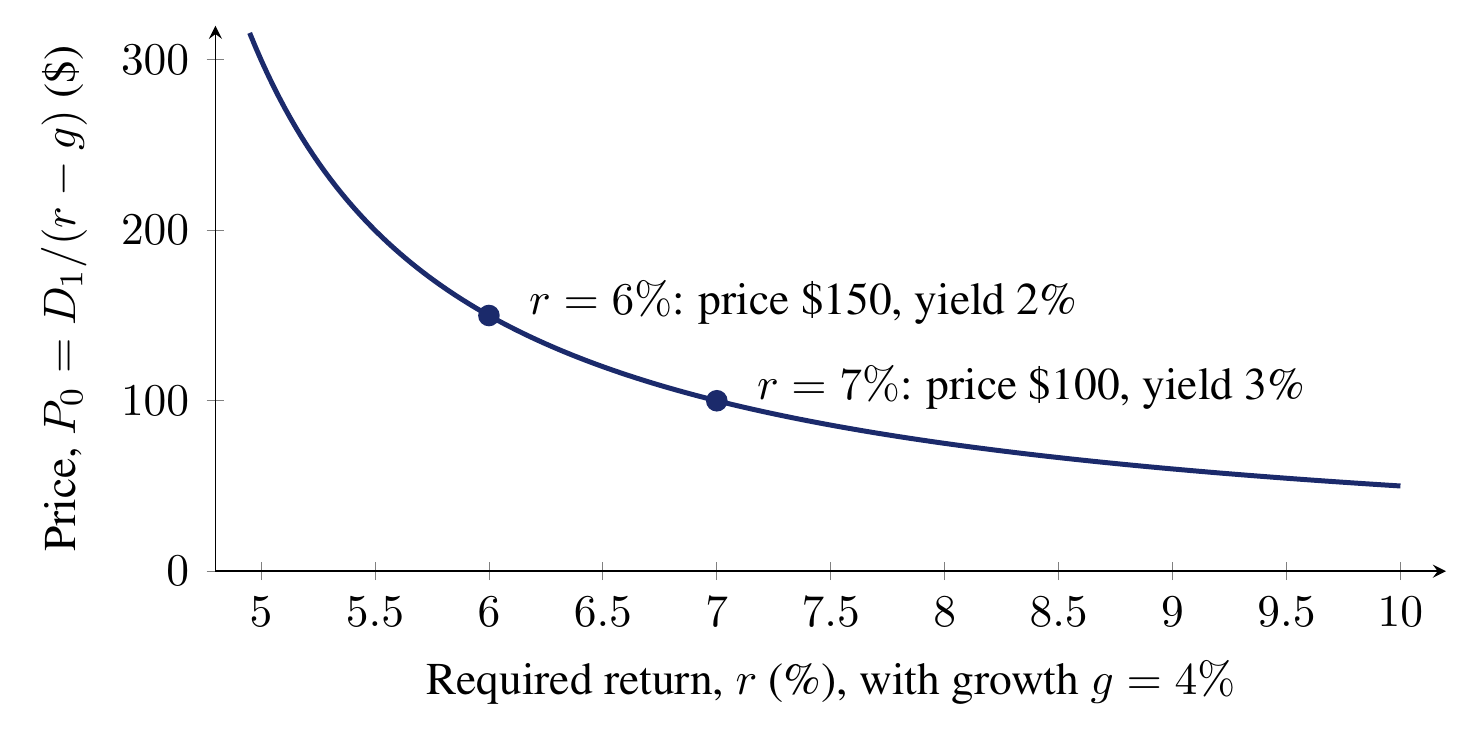
\includegraphics[width=0.85\linewidth]{images/fig07-1-gordon.png}
%\caption{The Gordon growth model for a market paying a \$3 dividend next year, with dividends growing 4\% a year. Lowering the required return from 7\% to 6\% raises the price from \$100 to \$150 and lowers the dividend yield from 3\% to 2\%. High prices and low yields go with low expected returns.}
%\label{fig:07-gordon}
%\end{figure}

\textbf{Expected and realized returns.} The required return $r$ in these formulas is an \textbf{expected return}: what investors anticipate, on average, when they buy. The \textbf{realized return} in any year is the expected return plus a surprise, and the surprises in stock returns are large. The \textbf{equity premium} is the expected return on stocks minus the risk-free rate; historically, U.S. stocks have earned a realized premium of roughly 6 to 8 percent a year over Treasury bills, though how much of that was expected is debated.

\textbf{Interest rates and the term structure.} The \textbf{yield} on a bond is the single discount rate that makes the present value of its promised payments equal to its price. Yields on government bonds of different maturities form the \textbf{term structure}, or \textbf{yield curve} (Figure~\ref{fig:07-curve}). The \textbf{term spread} is the yield on a long-term bond (say, 10 years) minus the yield on a short-term bill. The curve normally slopes upward; it tends to be steep near the bottom of recessions and flat or \textbf{inverted}, with short rates above long ones, before them. Hull's \emph{Options, Futures, and Other Derivatives} covers the term structure in detail; Chapter 16 tests what forward rates predict.

%\begin{figure}[htbp]
%\centering
%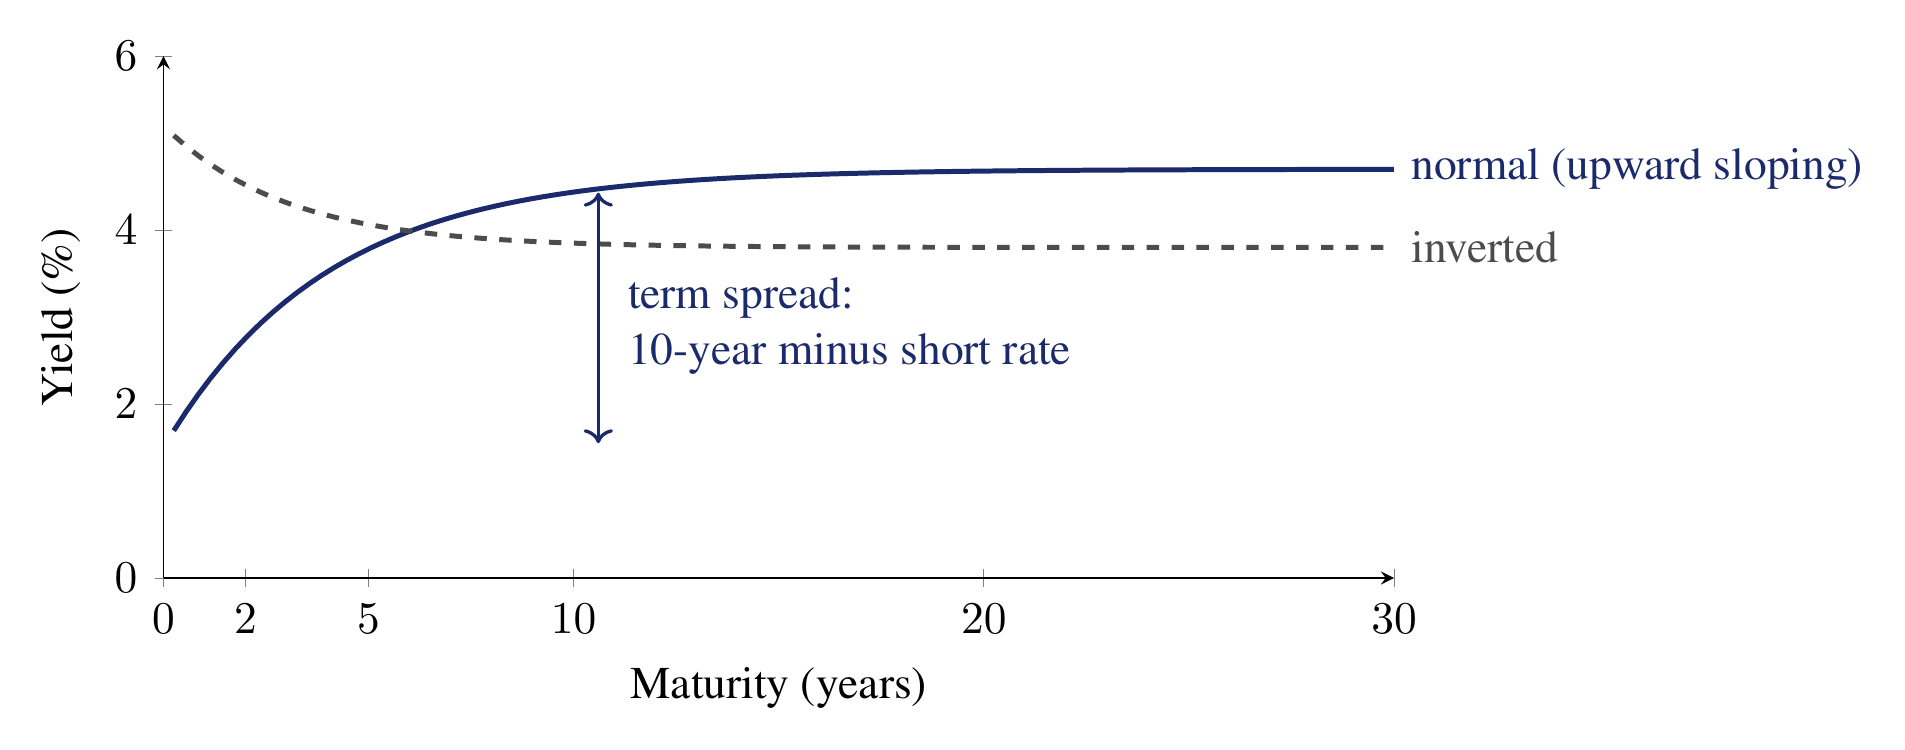
\includegraphics[width=0.85\linewidth]{images/fig07-2-yield-curves.png}
%\caption{Two shapes of the yield curve (illustrative). Normally, long-term yields exceed short-term ones and the term spread is positive. Before recessions the curve often flattens or inverts.}
%\label{fig:07-curve}
%\end{figure}

\textbf{Real and nominal.} \textbf{Nominal} returns and yields are in dollars; \textbf{real} returns subtract inflation, approximately $r_{real} \approx r_{nominal} - \text{inflation}$. A 5\% nominal return with 3\% inflation is about a 2\% real return. Stocks are claims on real businesses whose earnings tend to rise with prices over time, so their earnings yield behaves more like a real return. Government bond yields are nominal. Comparing the two directly, as the ``Fed model'' does, mixes the units.

\textbf{Worked example.} A market pays a dividend of \$3 next year on a price of \$100, a dividend yield of 3\%. If dividends are expected to grow 4\% a year, the Gordon model implies an expected return of $3\% + 4\% = 7\%$. If the price rose to \$150 with no change in expected growth, the yield would fall to 2\% and the implied expected return to 6\%.

\textbf{Further reading.} Berk and DeMarzo, \emph{Corporate Finance}, chapters on the time value of money and stock valuation; Bodie, Kane and Marcus, \emph{Investments}, chapters on equity valuation and the term structure; Cochrane, \emph{Asset Pricing}, chapter on time-series predictability of returns; Hull, \emph{Options, Futures, and Other Derivatives}, chapter on interest rates.

\section{How it works}
\label{sec:07-how}

\textbf{Valuation ratios.} A valuation ratio compares a stock market's price with a measure of what it pays or earns.

\begin{itemize}
  \item The \textbf{dividend--price ratio} divides the last twelve months of dividends by the index level.
  \item The \textbf{cyclically adjusted price--earnings ratio (CAPE)}, introduced by Campbell and Shiller (1988, 1998), divides the inflation-adjusted price by the average of inflation-adjusted earnings over the previous ten years. The ten-year average smooths out the swings of the \textbf{business cycle}, the alternation of expansions and recessions.
\end{itemize}

When prices are high relative to dividends or earnings, the market is said to be expensive.

\textbf{Why a valuation ratio should carry information.} The present-value identity of Campbell and Shiller (1988) links today's dividend--price ratio to the future. Approximately, and without any assumption about investor behavior,
\begin{equation}
  d_t - p_t \approx \text{constant} + \sum_{j=1}^{\infty} \rho^{j-1}\left(r_{t+j} - \Delta d_{t+j}\right)
  \label{eq:07-identity}
\end{equation}
where $d - p$ is the log dividend--price ratio, $r$ is the log return, $\Delta d$ is log dividend growth and $\rho$ is a constant slightly below one. In words: if prices are high relative to dividends today, then either future dividends must grow fast, or future returns must be low, or the ratio must stay high forever (Figure~\ref{fig:07-identity}). The identity does not say which. Whether returns are predictable is the question of which side of the identity does the work.


\providecolor{fenavy}{HTML}{1B2A6B}

\begin{figure}[!htbp]
  \centering
  \begin{tikzpicture}[
    % Illustrative yield curves (yield in %, maturity in years)
    declare function={
      normal(\x)   = 4.72 - 3.3*exp(-\x/2.9);
      inverted(\x) = 3.8 + 1.35*exp(-\x/2.5);
    }]
  \begin{axis}[
    width=0.58\linewidth, height=0.36\linewidth,
    scale only axis,
    axis lines=left,
    axis line style={-stealth, thin},
    xmin=0, xmax=30.5, ymin=0, ymax=6.2,
    xtick={0,2,5,10,20,30},
    ytick={0,2,4,6},
    xlabel={Maturity (years)},
    ylabel={Yield (\%)},
    samples=150, domain=0.3:30,
    clip=false,
  ]
    \addplot[fenavy, very thick] {normal(x)};
    \addplot[thick, dashed, gray!30!black] {inverted(x)};

    % Term spread: 10-year yield minus short rate, on the normal curve
    \draw[fenavy, thick, <->] (axis cs:10.5,{normal(0.3)}) -- (axis cs:10.5,{normal(10)});
    \node[fenavy, anchor=north west, align=left] at (axis cs:11,3.6)
      {term spread:\\10-year minus short rate};

    % Curve labels
    \node[fenavy, anchor=west] at (axis cs:30.3,{normal(30)}) {normal (upward sloping)};
    \node[gray!30!black, anchor=west] at (axis cs:30.3,{inverted(30)}) {inverted};
  \end{axis}
  \end{tikzpicture}
  \caption{Normal and inverted yield curves.}% <- replace with your caption
  \label{fig:07-yieldcurve}% <- replace with your label
\end{figure}


\providecolor{fenavy}{HTML}{1B2A6B}

\begin{figure}[!htbp]
  \centering
  \begin{tikzpicture}[
    csbox/.style={draw=fenavy, thick, rounded corners=2pt, align=center,
                  minimum width=3.6cm, minimum height=1.15cm, inner sep=4pt},
    csarr/.style={-stealth, thick},
  ]
    % Top: today's price relative to dividends
    \node[csbox, fill=fenavy!12, minimum width=4cm, minimum height=1.35cm] (cstop) at (0,0)
      {Prices high relative to\\dividends today};

    % Three outcomes
    \node[csbox] (csret) at (-4.3,-2.9) {future returns\\are low};
    \node[csbox] (csdiv) at (0,-2.9)    {future dividends\\grow fast};
    \node[csbox] (csbub) at (4.3,-2.9)  {the ratio stays\\high forever};

    \draw[csarr] (cstop.south) ++(-1,0) -- (csret.north);
    \draw[csarr] (cstop.south) -- (csdiv.north);
    \draw[csarr] (cstop.south) ++(1,0) -- (csbub.north);

    \node[fenavy, font=\small] at (-5.1,-1.45) {returns are predictable};

    \node[font=\small] at (0,-4.3)
      {at least one must happen; the identity does not say which};
  \end{tikzpicture}
  \caption{The Campbell--Shiller identity in words. A high price relative to
    dividends must be followed by low returns, fast dividend growth or a
    permanently high ratio. Return predictability is the first branch.}
  \label{fig:07-identity}
\end{figure}

%\begin{figure}[htbp]
%\centering
%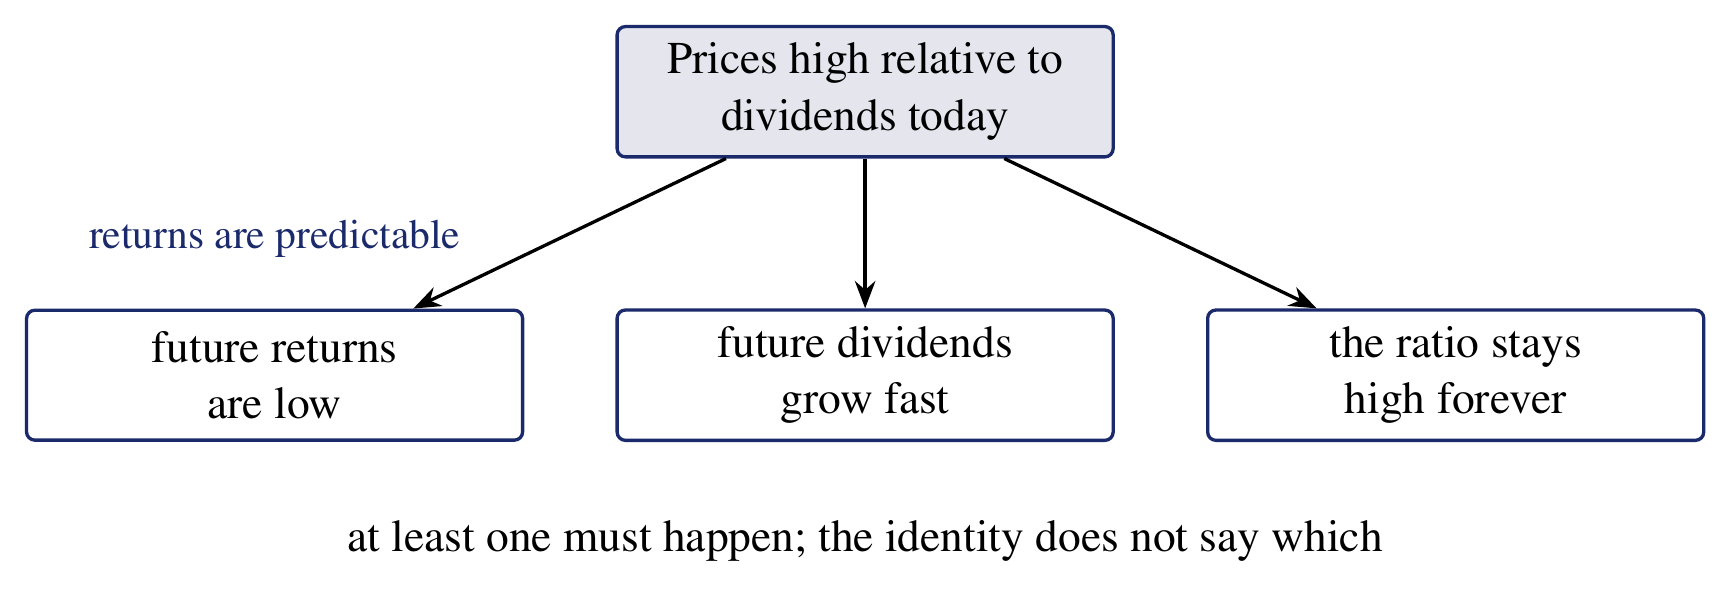
\includegraphics[width=0.85\linewidth]{images/fig07-3-identity.png}
%\caption{The Campbell--Shiller identity in words. A high price relative to dividends must be followed by low returns, fast dividend growth or a permanently high ratio. Return predictability is the first branch.}
%\label{fig:07-identity}
%\end{figure}

\textbf{Two readings of predictability.} If expected returns vary over time, there are two broad explanations:

\begin{itemize}
  \item \textbf{Rational time-varying risk premia.} In bad times investors are poorer, more \textbf{risk-averse} (less willing to bear risk) or more exposed to risk, so they demand higher expected returns; prices fall until expected returns are high enough. Predictability is then compensation, not a free lunch (Fama and French 1989; Cochrane 2008).
  \item \textbf{Behavioral mispricing.} Investors \textbf{extrapolate} recent good news, assuming it will continue; prices overshoot, and later returns are low as they correct. Predictability is then a sign of mispricing (Shiller 2000).
\end{itemize}

Both readings imply that high valuations precede low returns. They differ on whether an investor can profit by acting on that, which is the question this chapter tests.

\textbf{Predictive regressions.} The standard test regresses the return over the next $k$ months on today's predictor, as in Chapter 5. Because valuation ratios move slowly, regressions at long horizons use overlapping returns: each monthly observation of a 10-year return shares 119 months with the next. Chapter 3 showed how overlap inflates ordinary t-statistics; this chapter uses the corrections developed there.

\section{The claim}
\label{sec:07-claim}

Stated so that it can fail:

\begin{callout}
\textbf{Valuation ratios and macroeconomic variables forecast the U.S. equity premium well enough that an investor using them in real time would have done better than one assuming a constant expected return.}
\end{callout}

The last clause is what makes the claim testable. A pattern visible in the full history, with coefficients estimated using data the investor did not have, is not enough. The claim is about forecasts that could have been made.

The chapter tests four predictors, chosen because each has a large literature and a clear economic story:

\begin{center}
\small
\begin{tabularx}{0.9\linewidth}{@{}>{\raggedright\arraybackslash}p{0.30\linewidth}>{\raggedright\arraybackslash}p{0.20\linewidth}>{\raggedright\arraybackslash}X@{}}
\toprule
Predictor & Expected sign & Story \\
\midrule
Dividend--price ratio & High ratio, high returns & Cheap stocks pay more per dollar invested \\
CAPE (entered with its sign reversed) & High CAPE, low returns & Prices high relative to normal earnings must eventually fall back, or earnings rise \\
Term spread (long-term minus short-term yield) & Wide spread, high returns & The spread is high near business-cycle troughs, when risk premia are high (Fama and French 1989) \\
The ``Fed model'': earnings yield minus the 10-year Treasury yield & High spread, high returns & Stocks are cheap when their earnings yield exceeds bond yields \\
\bottomrule
\end{tabularx}
\end{center}

The claim is tested at three horizons: one month, one year and ten years. They correspond to three uses: tactical trading, annual asset allocation, and long-term planning.

\section{The original evidence}
\label{sec:07-evidence}

The case for predictability was built in three waves, and the case against it in a fourth.

\textbf{Valuation ratios (1987--1998).} Fama and French (1988) regressed U.S. stock returns on dividend yields and found that the explanatory power rose with the horizon: dividend yields explained little of monthly returns but often more than a quarter of the variance of returns over two to four years. Campbell and Shiller (1988) derived the present-value identity of Section~\ref{sec:07-how} and showed that dividend--price ratios and smoothed earnings forecast returns. Campbell and Shiller (1998), writing as U.S. valuations reached record highs, used ten-year average earnings, the measure now called CAPE, to argue that the market's expected returns over the following decade were unusually low. Shiller had presented similar evidence to the Federal Reserve Board in December 1996, days before Alan Greenspan's ``irrational exuberance'' speech.

\textbf{Business-cycle variables (1986--1989).} Keim and Stambaugh (1986), Campbell (1987) and Fama and French (1989) found that interest-rate spreads also predicted returns: notably the term spread between long- and short-term yields, and the \textbf{default spread} between the yields of low- and high-grade corporate bonds. Fama and French linked the pattern to the business cycle: expected returns were high near \textbf{troughs}, the low points of recessions, when spreads were wide and investors' willingness to bear risk was low. Their interpretation made predictability compatible with efficient markets, as time-varying compensation for risk.

\textbf{A consensus forms.} By the early 2000s, predictability from valuation ratios was widely taught as a stylized fact, and Cochrane's (2011) presidential address to the American Finance Association built a research agenda on the premise that discount rates, not expected cash flows, account for most of the movement in valuations.

\textbf{The challenge (1999--present).} Statisticians had warned that the evidence was fragile.

\begin{itemize}
  \item Stambaugh (1999) showed that persistent predictors whose surprises are correlated with returns bias slopes and t-statistics in finite samples.
  \item Valkanov (2003) and Boudoukh, Richardson and Whitelaw (2008) showed that long-horizon regressions add little information beyond short-horizon ones: the rising $R^2$ is largely a mechanical consequence of overlapping data and persistent predictors.
  \item Ang and Bekaert (2007), using data from several countries, found that long-horizon predictability from dividend yields largely disappeared once standard errors were corrected, while dividend yields helped at short horizons in combination with short-term interest rates.
  \item Goyal and Welch (2008) showed that almost none of the published predictors beat the historical mean in walk-forward forecasts, and Goyal, Welch and Zafirov (2024) found the same for predictors proposed since.
\end{itemize}

The defense did not concede. Campbell and Thompson (2008) showed that simple economic restrictions improve out-of-sample performance and that tiny $R^2$ values can be economically valuable. Cochrane (2008) argued that the absence of dividend-growth predictability implies return predictability through the present-value identity, so the evidence should be judged jointly rather than one regression at a time.

\section{Replication lab: Lab 7}
\label{sec:07-lab}

\begin{callout}
\textbf{Lab 7 at a glance.} \emph{The question:} do the dividend--price ratio, CAPE, the term spread and the Fed-model spread predict U.S. stock returns at horizons of one month, one year and ten years, in-sample and in real time? \emph{Data:} the Goyal--Welch monthly data from 1927, the same file as Lab 5, which includes the S\&P 500 index, twelve-month dividends and earnings, Treasury yields, inflation and CRSP total returns. CAPE is built from the index, earnings and inflation; it begins in 1923, once ten years of inflation-adjusted earnings are available. Optionally, Robert Shiller's long-run file extends CAPE and real returns back to 1881 for the ten-year analysis. \emph{Code:} repository folder \texttt{ch07-predictability/}, with a guided notebook.
\end{callout}

\textbf{The setup.}

\begin{itemize}
  \item \textbf{Part A, replication.} Regressions of future log excess returns on each predictor at each horizon, with three t-statistics: ordinary least squares, which ignores the overlap; Newey--West with lags equal to the horizon minus one; and Hodrick's (1992) standard errors, which avoid overlapping errors altogether. Figure 7.4 shows the classic pattern to look for: $R^2$ rising with the horizon.
  \item \textbf{Part B, walk-forward.} Forecasts from January 1965 using only data available at each date, with training observations purged when their targets had not yet been observed (Chapter 5). Out-of-sample $R^2$ against the historical mean, the Clark--West test, and the Campbell--Thompson restrictions. Figure 7.5 sets these beside the in-sample results.
  \item \textbf{Part C, stress tests.} Section~\ref{sec:07-stress} describes these.
  \item \textbf{Part D, ranges.} Annualized ten-year real returns regressed on starting CAPE, with the walk-forward forecast error used to set an honest range around the forecast for today's CAPE (Figure 7.8).
\end{itemize}

\textbf{What readers will find.} The lab reports every number from the data the reader supplies, so the results update as the data do. The pattern to test is the one the literature reports: in-sample $R^2$ of around 1\% at one month, larger at one year, and large at ten years; out-of-sample $R^2$ near or below zero at the short horizons for most predictors; and a ten-year relationship with CAPE that holds out of sample but leaves a range several percentage points wide. When the lab was run on simulated data in which the dividend--price ratio has weak true predictive power, the bootstrap of Part C showed why the published t-statistics overstate the evidence: the 95\% critical value under the null was about 2.6 rather than the textbook 1.645.

\section{Stress tests}
\label{sec:07-stress}

Four stress tests apply the earlier chapters' tools to the claim.

\textbf{1. Overlapping data (Chapter 3).} At the ten-year horizon, consecutive monthly observations share 119 of their 120 months. A century of data contains only about ten non-overlapping decades. Ordinary t-statistics treat the 1,000-plus overlapping observations as if they were independent and can overstate significance many times over. The lab reports OLS, Newey--West and Hodrick t-statistics side by side; the gap between the first and the others is the size of the overlap problem.

\textbf{2. The Stambaugh bias.} Valuation ratios are extremely persistent, and their surprises are strongly negatively correlated with return surprises: when prices jump, the dividend--price ratio falls. In finite samples this biases the estimated slope upward and makes t-statistics too large (Stambaugh 1999; Nelson and Kim 1993). The lab measures the bias directly with a bootstrap: it keeps each predictor's persistence and the correlation of its surprises with returns, but rebuilds returns with no predictability at all, and runs the same regression on 500 artificial histories. Figure 7.7 shows the resulting distribution of t-statistics under the null, which is shifted to the right of zero, and compares the actual t-statistic with that distribution rather than with the textbook normal.

\textbf{3. Different decades.} A relationship that reflects a stable economic mechanism should appear in different periods. The lab estimates each predictor's one-year slope in three subperiods (1927--1964, 1965--1994 and 1995 onward) and over rolling 20-year windows (Figure 7.6). The dividend--price ratio is the classic test case: the ratio fell to record lows in the late 1990s while returns stayed high, and many studies find that its slope and significance depend heavily on whether that period is included.

\textbf{4. Out of sample and with restrictions (Chapter 5).} Walk-forward forecasts with purging, the Clark--West test, and the Campbell--Thompson restrictions. These are the decisive tests for the claim as stated, because the claim is about forecasts an investor could have made.

\textbf{What the stress tests do not cover.} All four use U.S. data. International evidence is weaker and more mixed, which matters because the U.S. market's history is one of the most successful on record, a selection problem Chapter 2 discussed. The open questions in Section~\ref{sec:07-open} return to this.

\section{Verdict}
\label{sec:07-verdict}

The verdict depends on the horizon and on what the predictions are for. Based on the published evidence through the Goyal--Welch--Zafirov sample, and to be confirmed by readers' runs of Lab 7 on data through 2025:

\begin{center}
\small
\begin{tabularx}{0.9\linewidth}{@{}>{\raggedright\arraybackslash}p{0.21\linewidth}>{\raggedright\arraybackslash}p{0.11\linewidth}>{\raggedright\arraybackslash}p{0.13\linewidth}>{\raggedright\arraybackslash}X@{}}
\toprule
Use & Horizon & Verdict & Why \\
\midrule
Market timing: moving in and out of stocks & 1 month to 1 year & \textbf{Fails} & In-sample t-statistics shrink after correcting for overlap and the Stambaugh bias; walk-forward forecasts rarely beat the historical mean, and the predictors that help do so only in some decades \\
Long-run planning: setting expected-return assumptions & 10 years & \textbf{Survives, weakly} & High CAPE has been followed by lower ten-year returns, a pattern that has generally held up in walk-forward tests, but with roughly ten independent decades of evidence the relationship is imprecise and the honest range is several percentage points wide \\
The Fed model as a valuation signal & Any & \textbf{Fails} & Comparing a real earnings yield with a nominal bond yield has no sound economic basis, and it has not forecast returns \\
\bottomrule
\end{tabularx}
\end{center}

The verdict on the claim as stated, that these variables forecast the equity premium well enough to beat a constant expected return in real time, is therefore \textbf{fails for market timing}, with a narrower claim, that valuations shift the distribution of decade-long returns, surviving weakly. The verdict is dated by the sample tested and should be revisited as data accumulate: a decade of new returns adds one new independent observation to the ten-year evidence.

\section{What investors can use}
\label{sec:07-investors}

The useful lesson from a century of debate is not a timing signal but a planning input.

\begin{itemize}
  \item \textbf{Set long-run return assumptions with valuations in mind.} A retirement plan, an endowment's spending rule or a pension's discount rate that assumes the historical average return regardless of starting valuations ignores the most robust part of this evidence. When CAPE is high, plan for lower decade-long returns; when it is low, higher ones.
  \item \textbf{Plan for the range, not the point.} Lab 7's Part D reports a 90\% range for the next decade's annualized real return. The range is wide, typically several percentage points either side of the central forecast, and the plan should work across it.
  \item \textbf{Do not trade on it.} Valuations have been high, or low, for years at a time before returns responded. An investor who reduced equities whenever CAPE looked expensive would often have spent long periods underinvested while the market rose.
  \item \textbf{Distrust precise forecasts.} Any forecast of next year's market return stated to a decimal place, or a valuation ``fair value'' target for the index, implies a precision this evidence does not support.
\end{itemize}

\textbf{Questions to ask a fund manager or adviser who times the market with valuations:}

\begin{enumerate}
  \item Were your signals and their thresholds chosen before the period you are showing me? What did you try and discard?
  \item How did the strategy perform in real time, after it was designed, not in a backtest?
  \item What t-statistics do you get after correcting for overlapping returns and the persistence of your predictor?
  \item How long has the signal been wrong in the past, and could I bear being out of the market for that long?
  \item What is the strategy's out-of-sample $R^2$ against simply assuming the average return?
\end{enumerate}

\begin{callout}
\textbf{What Failed: the Fed model.} In July 1997 the Federal Reserve's Monetary Policy Report to Congress included a chart comparing the stock market's earnings yield with the ten-year Treasury yield. The strategist Ed Yardeni named the comparison the ``Fed model'': stocks are cheap when their earnings yield is above bond yields and expensive when below. The Fed never endorsed it, but it became one of Wall Street's most quoted valuation tools. Asness (2003) argued that it rests on a confusion: earnings yields are real quantities, because earnings grow with inflation, while bond yields are nominal, so comparing them builds in \textbf{money illusion}, the mistake of treating nominal and real amounts as the same, of the kind Modigliani and Cohn (1979) described. Its empirical record matches the logic. Asness found that it described how investors set prices but not what returns followed, and it had little power to forecast long-run returns. The relationship it relies on was also unstable: from the late 1990s, bond yields and earnings yields moved in opposite directions for long periods. The claim that the Fed model identifies when stocks are cheap \textbf{fails}. Lab 7 includes it as a fourth predictor so readers can check.
\end{callout}

\section{Open questions}
\label{sec:07-open}

\begin{itemize}
  \item \textbf{International evidence.} Do valuation ratios predict long-run returns outside the United States, using long histories for many countries? The answer bears on whether U.S. evidence reflects a mechanism or one fortunate market.
  \item \textbf{Changes in payout policy.} Share buybacks have replaced much of the dividend payout since the 1980s, which may have shifted the dividend--price ratio's level permanently. How should valuation ratios be adjusted, and does adjustment restore their predictive power?
  \item \textbf{Accounting changes in earnings.} Changes in accounting rules, such as write-down rules for goodwill, affect reported earnings and therefore CAPE. How large are these effects, and how should a long-run series correct for them?
  \item \textbf{Real-time data.} Lab 7 uses earnings as dated in the data file, not as first reported. How much does using genuinely real-time earnings change the evidence?
  \item \textbf{Combining signals.} Do forecast combinations, Bayesian methods that impose economic priors, or machine-learning models (Chapter 21) deliver forecasts that survive the stress tests of this chapter?
\end{itemize}

\section*{Exercises}
\addcontentsline{toc}{section}{Exercises}

\subsection*{Conceptual (all readers)}

\begin{enumerate}
  \item Use the present-value identity of Section~\ref{sec:07-how} to explain why a high dividend--price ratio must be followed by high returns, high dividend growth, or a permanently high ratio. Which of these does the evidence favor?
  \item Explain why the $R^2$ of a regression of 10-year returns on a persistent predictor can be large even if the predictor has little information about 1-month returns.
  \item Why does the Stambaugh bias push t-statistics up for the dividend--price ratio, and why would it push them the other way for a predictor whose surprises were positively correlated with returns?
  \item An adviser says CAPE predicts that the next ten years will deliver 3\% a year after inflation. What information is missing from that statement?
\end{enumerate}

\subsection*{Lab extensions (technical readers)}

\begin{enumerate}
  \setcounter{enumi}{4}
  \item Re-run Lab 7 ending in 1990 (\texttt{-{}-end 1990-12}), roughly the data available to the original authors. Then run it from 1991. How different are the conclusions?
  \item Compare the OLS, Newey--West and Hodrick t-statistics for the 10-year horizon. By what factor does ignoring overlap overstate significance?
  \item Lag CAPE by four months to allow for delays in reported earnings. Does the evidence change?
  \item Supply Shiller's data and repeat Part D from 1881. How does the longer history change the slope and the width of the range?
  \item Obtain long-run data for another country's stock market and repeat Part D. Does the CAPE relationship hold?
  \item Build a combination forecast of the four predictors, as in Rapach, Strauss and Zhou (2010), and evaluate it with the stress tests of Section~\ref{sec:07-stress}.
\end{enumerate}

\section*{References}
\addcontentsline{toc}{section}{References}

\begin{itemize}
  \item Ang, A. and Bekaert, G. (2007). Stock Return Predictability: Is It There? \emph{Review of Financial Studies} 20(3): 651--707.
  \item Asness, C. S. (2003). Fight the Fed Model. \emph{Journal of Portfolio Management} 30(1): 11--24.
  \item Boudoukh, J., Richardson, M. and Whitelaw, R. F. (2008). The Myth of Long-Horizon Predictability. \emph{Review of Financial Studies} 21(4): 1577--1605.
  \item Campbell, J. Y. (1987). Stock Returns and the Term Structure. \emph{Journal of Financial Economics} 18(2): 373--399.
  \item Campbell, J. Y. and Shiller, R. J. (1988). The Dividend-Price Ratio and Expectations of Future Dividends and Discount Factors. \emph{Review of Financial Studies} 1(3): 195--228.
  \item Campbell, J. Y. and Shiller, R. J. (1998). Valuation Ratios and the Long-Run Stock Market Outlook. \emph{Journal of Portfolio Management} 24(2): 11--26.
  \item Campbell, J. Y. and Thompson, S. B. (2008). Predicting Excess Stock Returns Out of Sample: Can Anything Beat the Historical Average? \emph{Review of Financial Studies} 21(4): 1509--1531.
  \item Cochrane, J. H. (2008). The Dog That Did Not Bark: A Defense of Return Predictability. \emph{Review of Financial Studies} 21(4): 1533--1575.
  \item Cochrane, J. H. (2011). Presidential Address: Discount Rates. \emph{Journal of Finance} 66(4): 1047--1108.
  \item Fama, E. F. and French, K. R. (1988). Dividend Yields and Expected Stock Returns. \emph{Journal of Financial Economics} 22(1): 3--25.
  \item Fama, E. F. and French, K. R. (1989). Business Conditions and Expected Returns on Stocks and Bonds. \emph{Journal of Financial Economics} 25(1): 23--49.
  \item Goyal, A. and Welch, I. (2008). A Comprehensive Look at the Empirical Performance of Equity Premium Prediction. \emph{Review of Financial Studies} 21(4): 1455--1508.
  \item Goyal, A., Welch, I. and Zafirov, A. (2024). A Comprehensive 2022 Look at the Empirical Performance of Equity Premium Prediction. \emph{Review of Financial Studies} 37(11): 3490--3557.
  \item Hodrick, R. J. (1992). Dividend Yields and Expected Stock Returns: Alternative Procedures for Inference and Measurement. \emph{Review of Financial Studies} 5(3): 357--386.
  \item Keim, D. B. and Stambaugh, R. F. (1986). Predicting Returns in the Stock and Bond Markets. \emph{Journal of Financial Economics} 17(2): 357--390.
  \item Modigliani, F. and Cohn, R. A. (1979). Inflation, Rational Valuation and the Market. \emph{Financial Analysts Journal} 35(2): 24--44.
  \item Nelson, C. R. and Kim, M. J. (1993). Predictable Stock Returns: The Role of Small Sample Bias. \emph{Journal of Finance} 48(2): 641--661.
  \item Rapach, D. E., Strauss, J. K. and Zhou, G. (2010). Out-of-Sample Equity Premium Prediction: Combination Forecasts and Links to the Real Economy. \emph{Review of Financial Studies} 23(2): 821--862.
  \item Shiller, R. J. (2000). \emph{Irrational Exuberance}. Princeton, NJ: Princeton University Press.
  \item Stambaugh, R. F. (1999). Predictive Regressions. \emph{Journal of Financial Economics} 54(3): 375--421.
  \item Valkanov, R. (2003). Long-Horizon Regressions: Theoretical Results and Applications. \emph{Journal of Financial Economics} 68(2): 201--232.
\end{itemize}

\textbf{Data:} Goyal--Welch monthly predictor data, updated through 2025, from \url{https://sites.google.com/view/agoyal145}. Robert Shiller, U.S. stock market data 1871--present and CAPE, \url{http://www.econ.yale.edu/~shiller/data.htm}.

% Chapter 8 -- Claim: Value Beats Growth
% Requires: amsmath, amssymb, booktabs, array, tabularx, graphicx, tcolorbox (breakable, skins), hyperref or url.
% Defines the callout box only if the preamble has not.
\providecolor{fenavy}{HTML}{1B2A6B}
\providecolor{feshade}{HTML}{F3F5FA}
\makeatletter
\@ifundefined{callout}{%
  \newtcolorbox{callout}{breakable, enhanced,
    colback=white, colframe=gray!70, boxrule=0.5pt, arc=1mm,
    borderline west={2.5pt}{0pt}{gray!70},
    left=8pt, right=8pt, top=4pt, bottom=4pt}%
}{}
\makeatother

\chapter{Claim: Value Beats Growth}
\label{ch:08}

Buying what is cheap is the oldest idea in investing. Benjamin Graham taught it in the 1930s (Graham and Dodd 1934), Warren Buffett built a fortune on a refined version of it, and in the early 1990s academic finance gave it a name, a number and a factor: the value premium, measured by HML. For three decades afterward, a tilt toward value stocks was one of the most widely recommended departures from the market portfolio, built into index funds, smart-beta products and the asset allocations of large institutions.

Then, from about 2007, value stopped working in the United States. For more than a decade expensive growth stocks beat cheap value stocks by a wide margin, and the debate turned from why value works to whether it ever did, whether it had been arbitraged away, or whether accounting had changed what ``cheap'' means.

This chapter puts the claim on trial with a century of U.S. data, other measures of cheapness, other countries and the investor's own question: even if the premium is real, could you have held on long enough to collect it?

By the end of the chapter you will be able to:

\begin{itemize}
  \item compute book-to-market and other valuation ratios, and explain why intangible investment distorts book value;
  \item explain what an anomaly is, and how portfolio sorts and long--short factors are built;
  \item construct HML from the six size and book-to-market portfolios;
  \item compare the risk and mispricing explanations of the value premium;
  \item state the claim that value beats growth in a form that can fail, and test it over time, across measures, among large stocks, abroad and after costs;
  \item size a value tilt you could hold through a decade of underperformance.
\end{itemize}

\section{Foundations: accounting value, anomalies and factor portfolios}
\label{sec:08-foundations}

\textbf{Book value and market value.} A firm's \textbf{book value of equity} is an accounting figure from its \textbf{balance sheet}, the statement of what a firm owns and owes: total assets minus total liabilities, built mainly from the historical cost of what the firm has invested, less \textbf{depreciation}, the gradual write-down of assets as they wear out. Its \textbf{market value of equity} is the share price times shares outstanding: what investors think the firm's future cash flows are worth today. The ratio of the two, \textbf{book-to-market} (or its inverse, price-to-book), compares what the firm has put in with what the market expects it to earn.

Accounting rules record spending on factories and equipment as assets, but treat most spending on research, software, brands and training as expenses that reduce earnings and never appear on the balance sheet. Firms that invest mainly in such \textbf{intangible} assets therefore tend to have low book values relative to their market values (Figure~\ref{fig:08-book}).

\textbf{Other valuation ratios.} Each of these measures how much the investor gets per dollar paid:

\begin{itemize}
  \item \textbf{earnings-to-price} (the inverse of the P/E ratio) compares annual profits with the share price;
  \item \textbf{cash flow-to-price} uses earnings plus depreciation and other non-cash charges;
  \item \textbf{dividend yield} uses dividends paid.
\end{itemize}

Stocks high on these ratios are called \textbf{value} stocks, those low on them \textbf{growth} stocks.

\textbf{The CAPM and its failures.} The capital asset pricing model says that a stock's expected excess return is its market beta times the market's expected excess return (Chapter 3). A stock's \textbf{alpha} is the part of its average return the model does not explain. From the late 1970s, researchers found that stocks with high earnings-to-price or book-to-market ratios had positive alphas: they earned more than their betas justified. These became known as \textbf{anomalies}, patterns the CAPM could not explain.

\textbf{Portfolio sorts.} The standard empirical method for studying a characteristic like book-to-market is a \textbf{portfolio sort}:

\begin{enumerate}
  \item at regular intervals, rank all stocks on the characteristic;
  \item group them into portfolios: deciles (ten groups), quintiles (five) or the 30/40/30 split used for HML;
  \item hold each portfolio for a period, and record its return.
\end{enumerate}

A \textbf{long--short} or \textbf{high-minus-low} portfolio buys the top group and sells the bottom one. If the characteristic is related to expected returns, the long--short portfolio will earn a positive average return.

\textbf{Factors and factor models.} When a long--short portfolio captures a pattern shared by many stocks, it can serve as a \textbf{factor} in a model of expected returns. The Fama--French three-factor model explains expected excess returns with the market, a size factor (SMB) and a value factor (HML). A stock's or fund's \textbf{loadings} on these factors, estimated by regression, describe its style; its alpha relative to the model measures what the factors do not explain.

\textbf{Worked example.} A company has book equity of \$2 billion and 100 million shares trading at \$50, a market value of \$5 billion. Its book-to-market ratio is $2/5 = 0.4$ and its price-to-book ratio 2.5. If it had spent \$1 billion on research over the past five years that accounting treated as expenses, and that spending were instead counted as an asset, its adjusted book-to-market would be closer to $3/5 = 0.6$.

\begin{figure}[htbp]
\centering
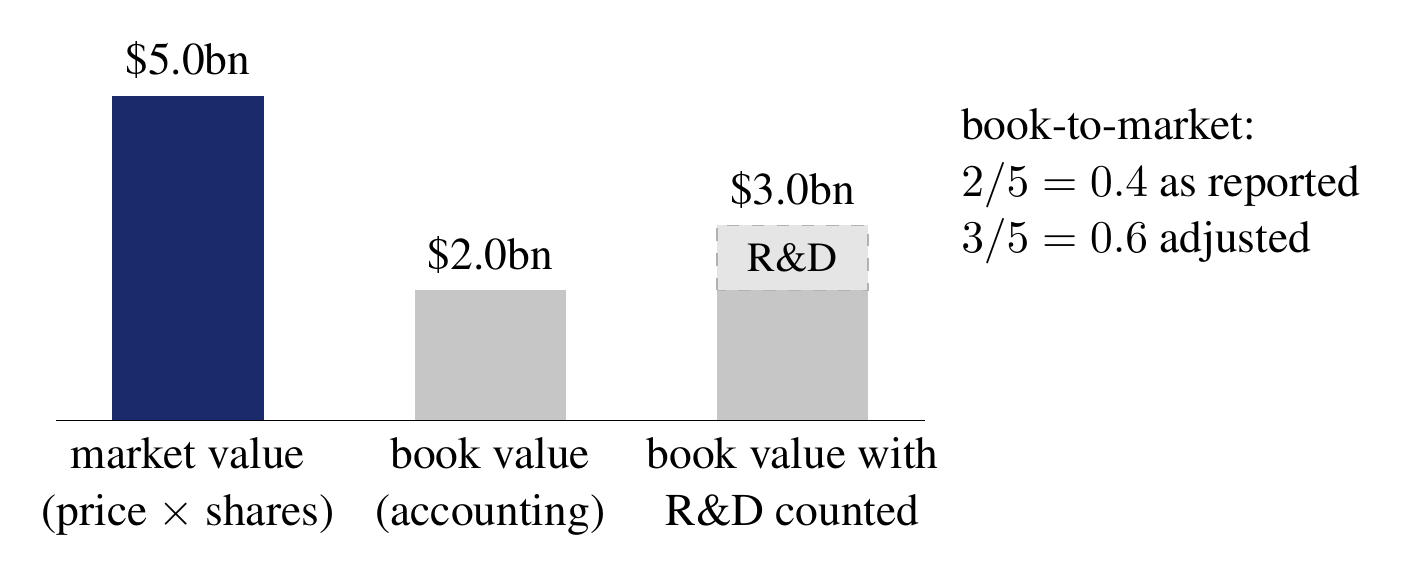
\includegraphics[width=0.85\linewidth]{images/fig08-1-book-market.png}
\caption{Book value, market value and intangibles, from the worked example. Counting past research spending as an asset raises book value from \$2 billion to \$3 billion and book-to-market from 0.4 to 0.6, moving the firm toward the value end of a sort.}
\label{fig:08-book}
\end{figure}

\textbf{Further reading.} Bodie, Kane and Marcus, \emph{Investments}, chapters on financial statement analysis, the CAPM, multifactor models and market efficiency; Bali, Engle and Murray, \emph{Empirical Asset Pricing}, chapters on portfolio sorts and the value effect; Cochrane, \emph{Asset Pricing}, chapter on the cross-section of returns; Ilmanen, \emph{Expected Returns}, chapter on the value premium.

\section{How it works}
\label{sec:08-how}

\textbf{Measuring cheapness.} A value stock is one whose price is low relative to a fundamental measure of the firm. The most studied measure is the book-to-market ratio. Other measures divide earnings, cash flow, dividends or sales by price. Each tells a slightly different story: book value measures past investment, earnings measure current profitability, dividends measure payouts.

\textbf{Sorting into portfolios.} The academic approach sorts all stocks on the chosen ratio and compares the returns of the cheapest group with the most expensive. Fama and French's \textbf{HML} (``high minus low'') factor does this carefully (Figure~\ref{fig:08-hml}):

\begin{enumerate}
  \item Each June, stocks are split into small and big by market value, and into three groups by book-to-market: growth (bottom 30\%), neutral and value (top 30\%).
  \item Six value-weighted portfolios result: small growth, small neutral, small value, big growth, big neutral, big value.
  \item HML is the average return of the two value portfolios minus the average return of the two growth portfolios. It is long cheap stocks and short expensive ones, with equal weight on small and big firms.
\end{enumerate}

\begin{figure}[htbp]
\centering
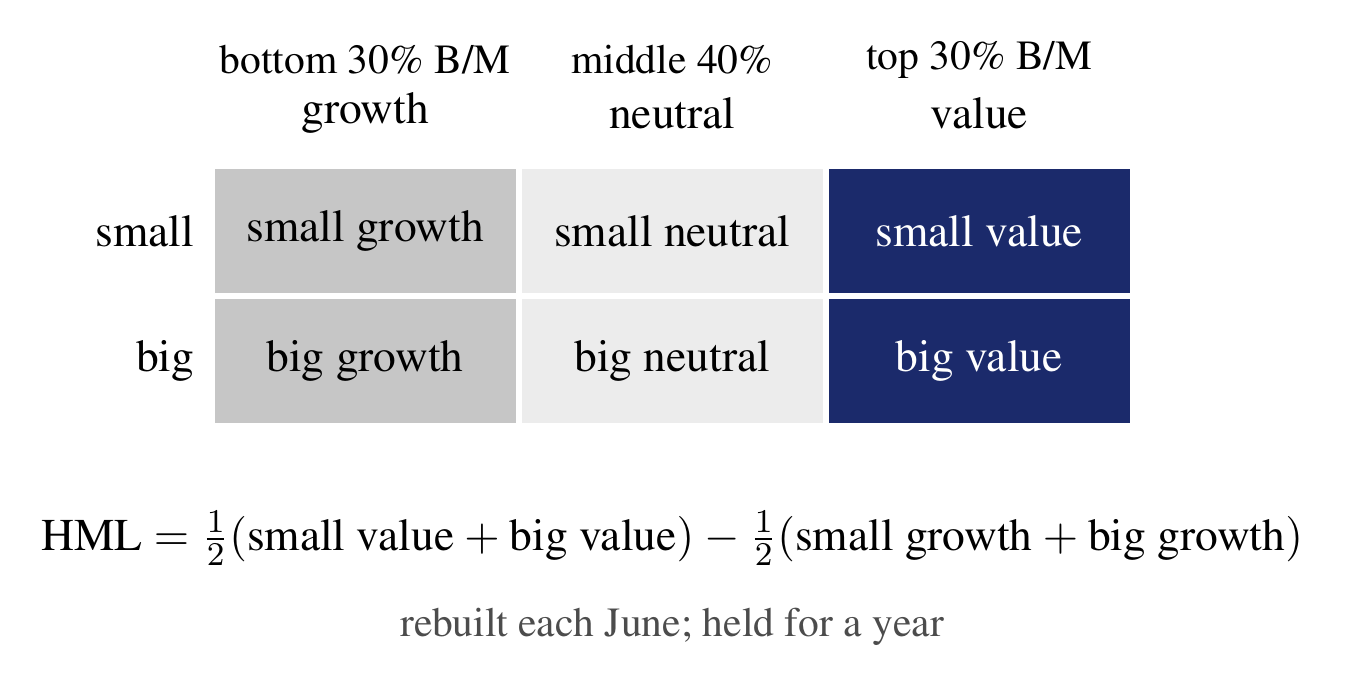
\includegraphics[width=0.85\linewidth]{images/fig08-2-hml.png}
\caption{How HML is built. Stocks are sorted into two size groups and three book-to-market groups. HML buys the two value portfolios and sells the two growth portfolios, so that small and big firms count equally.}
\label{fig:08-hml}
\end{figure}

The portfolios are held for a year and rebuilt the next June, using book equity from the fiscal year ending in the previous calendar year so that the accounting data would have been public (Section~\ref{sec:02-lookahead}). This design keeps HML's turnover low, about 3\% a month (Chapter 6; Novy-Marx and Velikov 2016).

\textbf{Why value might earn more.} Two families of explanation compete:

\begin{itemize}
  \item \textbf{Risk.} Value firms are often distressed or inflexible: they have assets in place that are hard to cut back in recessions. If they do worst in bad economic times, investors demand higher expected returns to hold them (Fama and French 1993; Zhang 2005).
  \item \textbf{Mispricing.} Investors extrapolate past growth too far into the future, overpaying for glamorous growth firms and shunning unexciting value firms. As the expected growth fails to arrive, prices correct (Lakonishok, Shleifer and Vishny 1994).
\end{itemize}

The distinction matters for the future. A risk premium should persist, though it may arrive unevenly. A mispricing can shrink as investors learn about it and as capital flows in to exploit it.

\section{The claim}
\label{sec:08-claim}

Stated so that it can fail:

\begin{callout}
\textbf{Stocks that are cheap relative to fundamentals earn higher average returns than expensive stocks, by enough to matter after costs, in data beyond the samples that established the result.}
\end{callout}

The last clause is the key. The value premium is well documented in the data that discovered it. The question is whether it held afterward, in other markets, with other measures, and at a size an investor could hold. Three tests follow from the claim:

\begin{itemize}
  \item \textbf{Time.} Does HML earn a positive premium after the original sample of Fama and French (1992), which ended in 1990, and in particular after 2007?
  \item \textbf{Breadth.} Does the premium appear with earnings, cash flow and dividends as well as book value, among large stocks as well as small ones, and in other countries?
  \item \textbf{Implementability.} Does it survive costs, and could an investor live with its \textbf{drawdowns}, the falls from a previous peak, long enough to collect it?
\end{itemize}

\section{The original evidence and its interpretations}
\label{sec:08-evidence}

\textbf{Before the factor.} Basu (1977) found that stocks with high earnings-to-price ratios earned higher risk-adjusted returns than the capital asset pricing model predicted. Rosenberg, Reid and Lanstein (1985) found the same for book-to-market. These were treated as anomalies: puzzles for the CAPM rather than a new principle.

\textbf{Fama and French (1992, 1993).} Using U.S. stocks from 1963 to 1990, Fama and French (1992) showed that size and book-to-market together captured the \textbf{cross-section of average returns}, the differences in average return across stocks, and that market beta, the CAPM's only variable, added nothing. Fama and French (1993) turned the finding into the three-factor model, with HML as the value factor, and interpreted it as compensation for a risk related to financial distress. The papers changed the field: the three-factor model became the standard benchmark for judging investment performance for two decades.

\textbf{Lakonishok, Shleifer and Vishny (1994)} offered the competing interpretation. Value stocks did not appear riskier in the ways that mattered: they did not do notably worse in bad markets or recessions. Instead, investors seemed to extrapolate past growth: \textbf{glamour} firms with strong past growth were priced as if it would continue, and it did not.

\textbf{Breadth.} Fama and French (1998) found value premiums in many international markets, and Asness, Moskowitz and Pedersen (2013) found value effects across countries and asset classes, from stocks to bonds to currencies to commodities. By the 2010s, value was one of the best-documented patterns in finance.

\textbf{The drought.} From 2007 to 2020, U.S. value stocks trailed growth stocks by a large cumulative margin, the longest and deepest drawdown in HML's history. Explanations multiplied.

\begin{itemize}
  \item \textbf{Mismeasured book value.} Book value had become a poor measure of a firm's assets because spending on research, software and brands is expensed rather than recorded as an asset. Eisfeldt, Kim and Papanikolaou (2022) showed that adding \textbf{capitalized} intangible investment, recorded as an asset rather than an expense, to book equity produced a value factor that performed substantially better, including in recent decades.
  \item \textbf{Interest rates and crowding.} Others pointed to falling interest rates, which raise the value of distant growth cash flows, or to crowding by investors following the same strategy.
  \item \textbf{Noise.} Fama and French (2021) split 1963--2019 in half and found much lower value premiums in the second half, especially among large stocks, but showed that the volatility of returns made it impossible to reject either that the premium was unchanged or that it had fallen to zero.
  \item \textbf{Revaluation.} Arnott, Harvey, Kalesnik and Linnainmaa (2021) argued that much of the drought reflected value stocks becoming cheaper relative to growth stocks, a revaluation that cannot continue indefinitely, rather than a disappearing premium.
\end{itemize}

\section{Replication lab: Lab 8}
\label{sec:08-lab}

\begin{callout}
\textbf{Lab 8 at a glance.} \emph{The question:} has HML earned a premium over the century of available U.S. data, and in particular since 2007? Does the answer depend on how cheapness is measured, on firm size, or on the country? \emph{Data:} Kenneth French's library: the Fama--French factors from July 1926; the six size and book-to-market portfolios; univariate portfolios formed on book-to-market, earnings-to-price, cash flow-to-price and dividend yield; and HML factors for North America, Europe, Japan, Asia Pacific ex Japan and the developed markets outside the United States, from 1990. Optionally, the Jensen--Kelly--Pedersen (2023) data extends the test to dozens of countries. \emph{Code:} repository folder \texttt{ch08-value/}, with a guided notebook.
\end{callout}

\textbf{The setup.}

\begin{itemize}
  \item \textbf{Part A, replication.} HML's average return, t-statistic, Sharpe ratio and CAPM alpha over the full sample and in four eras: 1926--1963, the original Fama--French sample of 1963--1990, 1991--2006, and 2007 to the present. A formal test asks whether the post-2007 premium differs from the earlier one by more than chance would allow.
  \item \textbf{Part B, stress tests.} Section~\ref{sec:08-stress} describes these.
  \item \textbf{Part C, other markets.} International HML before and after 2007.
  \item \textbf{Part D, living with value.} Drawdowns, the longest time spent below a previous peak, the worst ten-year period, and a bootstrap of ten-year outcomes used to size a value tilt (Section~\ref{sec:08-investors}).
\end{itemize}

\textbf{What readers will find.} Figure 8.3 shows the growth of a dollar in HML over the century, with the eras marked. Figure 8.4 sets out the premium in each era with its 95\% interval: the test of the claim over time is whether the post-2007 interval excludes the earlier premium, excludes zero, or neither. Fama and French's own split of 1963--2019 found the last of these, and readers can check whether the years since 2019 have changed the answer. Figure 8.7 shows how long value can disappoint, and Figure 8.8 turns that history into a range of ten-year outcomes.

\section{Stress tests}
\label{sec:08-stress}

\textbf{1. Other measures of cheapness.} If the value premium reflects something about cheap firms, it should appear whether cheapness is measured with book value, earnings, cash flow or dividends. If it appears only with book-to-market, it may be an artifact of accounting. The lab compares top-30\%-minus-bottom-30\% spreads for all four measures, over the full sample and before and after 2007. Book value is the measure most exposed to the intangibles problem, because research spending and brand building reduce book equity directly; earnings and cash flow are affected too, but less.

\textbf{2. Large stocks only.} Many anomalies are strongest among small stocks, which are expensive to trade and hold little of the market's value (Section~\ref{sec:02-microcaps}). The $2 \times 3$ portfolios separate value among big stocks from value among small stocks. Fama and French (2021) found that the decline in the second half of their sample was much larger for big stocks; the lab extends their comparison to the present.

\textbf{3. Intangible-adjusted book equity.} Eisfeldt, Kim and Papanikolaou (2022) capitalized research and development and a share of selling, general and administrative spending into book equity. Their intangible-adjusted value factor performed better throughout, including in the drought years. Replicating this requires firm-level accounting data that is not freely available, so the lab does not reproduce it; an exercise outlines how to do so with access to Compustat. Readers should note what the result implies: the drought was partly a measurement problem, not only a failure of the idea that cheap stocks earn more.

\textbf{4. After costs.} Value is a slow strategy. With turnover of about 3\% a month, a one-way trading cost of 20 to 50 basis points reduces its average return by roughly 0.3 to 0.7 percentage points a year (Equation~\eqref{eq:06-net}: $4 \times 0.03 \times 12 = 1.44$ times the one-way cost each year). Costs are not what threatens the value premium.

\textbf{5. Other countries.} If value works because of something general about how markets price cheap firms, it should appear outside the United States. The French international factors allow a test since 1990, before and after 2007. The Jensen--Kelly--Pedersen data, covering many more countries, also invites Chapter 4's warning: with dozens of countries, some will show significant premiums by chance, and some will show none.

\section{Verdict}
\label{sec:08-verdict}

Based on the published evidence through the end of the 2010s drought, to be confirmed by readers' runs of Lab 8 on data through 2025: \textbf{weakens.}

\begin{center}
\small
\begin{tabularx}{0.9\linewidth}{@{}>{\raggedright\arraybackslash}p{0.24\linewidth}>{\raggedright\arraybackslash}X>{\raggedright\arraybackslash}p{0.21\linewidth}@{}}
\toprule
Test & Finding & Effect on the claim \\
\midrule
Full century of U.S. data & HML earned a positive average premium, with a t-statistic well above conventional thresholds & Supports \\
After the original sample, and especially after 2007 & Much smaller, and for large U.S. stocks close to zero or negative over long stretches; statistically hard to distinguish either from the old premium or from zero & Weakens \\
Other measures of cheapness & The premium appears with earnings and cash flow as well as book value, though not identically & Supports breadth \\
Large stocks & Weaker than among small stocks, particularly in recent decades & Weakens \\
Intangible-adjusted book equity & A better-measured value factor performs better, including recently & Suggests part of the drought is mismeasurement \\
Other countries & Present in many markets, but uneven across countries and periods & Supports, with variation \\
Costs & Small relative to the premium & No effect \\
\bottomrule
\end{tabularx}
\end{center}

The claim that cheap stocks earn more than expensive ones has a century of support and a sound economic logic, but its size, its reliability and the measure of cheapness that captures it are all less certain than the field believed in the 1990s. The verdict is dated by the sample tested; a value premium that returned strongly for a decade would move it toward survives, and another decade like 2007--2020 toward fails.

\section{What investors can use}
\label{sec:08-investors}

The central lesson of value's history is not about its average return but about its patience requirement.

\textbf{Size the tilt you can hold through ten bad years.} A \textbf{value tilt} of weight $w$ adds $w$ times HML to a market portfolio, so its return relative to the market is $w$ times HML. Lab 8's Part D resamples HML's history to estimate a bad-case ten-year outcome, the 5th percentile, and reports the largest tilt whose bad case stays within a shortfall you specify. An investor who would abandon a strategy after trailing the market by 10\% over a decade should hold no larger a tilt than that, because abandoning it after the losses and before the recovery is the worst outcome of all.

\textbf{Expect long droughts.} Even if the premium is real, the lab's drawdown statistics show how long HML can spend below a previous peak. A premium that arrives once a decade, irregularly, is a premium most investors will not stay to collect.

\textbf{Prefer measures that are harder to distort.} Composite measures that combine several value signals, and book equity adjusted for intangible investment, are less exposed to accounting changes than raw book-to-market.

\textbf{Questions to ask a value manager:}

\begin{enumerate}
  \item Which measure of cheapness do you use, and how did it perform from 2007 to 2020?
  \item How much of your historical return comes from small stocks you could not hold at your current size?
  \item How do you handle firms whose book value omits most of their assets, such as software, pharmaceutical and brand-driven companies?
  \item What is your worst ten-year relative performance in your backtest and in live trading, and how did clients respond?
  \item Is your recent improvement a return of the premium, or value stocks becoming more expensive relative to growth?
\end{enumerate}

\begin{callout}
\textbf{What Failed: confident calls on value's death and its return.} As the drought deepened in the late 2010s, confident claims multiplied in both directions. Some declared value permanently dead, arbitraged away by the factor-investing industry or made obsolete by a technology-driven economy. Others declared, year after year, that a sharp comeback was imminent because value had become historically cheap relative to growth. Both claims ran ahead of the evidence. A premium whose year-to-year volatility is large relative to its average cannot be declared dead after a decade of losses, as Fama and French (2021) showed formally; and cheapness relative to growth, while it raises expected returns, says little about when they will arrive. Value rebounded strongly in 2021 and 2022 and then lagged again. The claim that anyone could confidently time value's death or its revival \textbf{fails}.
\end{callout}

\section{Open questions}
\label{sec:08-open}

\begin{itemize}
  \item \textbf{Has intangible investment changed what ``cheap'' means?} If so, what is the right measure of a firm's invested capital, and does a properly measured value premium look stable?
  \item \textbf{Risk or mispricing?} The drought is a natural experiment. Did value's losses coincide with bad times for investors, as a risk story would require, or with good times?
  \item \textbf{Interest rates.} How much of value's performance since 2007 is explained by falling, then rising, interest rates acting on the long-duration cash flows of growth firms?
  \item \textbf{International divergence.} Why has the value premium been more persistent in some markets, such as Japan, than in the United States?
  \item \textbf{Crowding.} Did the growth of value funds and factor products reduce the premium, and can crowding be measured in advance?
\end{itemize}

\section*{Exercises}
\addcontentsline{toc}{section}{Exercises}

\subsection*{Conceptual (all readers)}

\begin{enumerate}
  \item Explain the difference between the risk and mispricing explanations of the value premium. What evidence from the 2007--2020 drought would favor each?
  \item Why does HML use book equity from the previous fiscal year and rebalance only in June? What would go wrong with monthly rebalancing on the latest accounting data?
  \item A firm spends heavily on research and development. How does that spending affect its book-to-market ratio, and why might it be misclassified as a growth stock?
  \item Explain why a value premium of 4\% a year with 12\% annual volatility cannot be distinguished from zero over a 15-year period. How many years would be needed?
\end{enumerate}

\subsection*{Lab extensions (technical readers)}

\begin{enumerate}
  \setcounter{enumi}{4}
  \item Split the sample at 1990 instead of 2007. Which break looks more like a change in the premium?
  \item Compare value among large and small stocks after 2007. What does the comparison imply about who could actually have earned the premium?
  \item Run Part D with a tolerance of 5\% and 20\%. How does the largest tilt change, and what would you recommend to a cautious and to a patient investor?
  \item With the JKP data, count the countries in which the value premium has a t-statistic above 2. How many would you expect by chance?
  \item With access to firm-level accounting data, rebuild book equity by capitalizing research and development and part of selling, general and administrative spending, and rebuild HML. Does the post-2007 shortfall shrink?
  \item Measure the \textbf{value spread}, the gap in book-to-market between value and growth portfolios, over time. Does a wide spread predict higher subsequent HML returns? Apply Chapter 5's out-of-sample tests.
\end{enumerate}

\section*{References}
\addcontentsline{toc}{section}{References}

\begin{itemize}
  \item Arnott, R. D., Harvey, C. R., Kalesnik, V. and Linnainmaa, J. T. (2021). Reports of Value's Death May Be Greatly Exaggerated. \emph{Financial Analysts Journal} 77(1): 44--67.
  \item Asness, C. S., Moskowitz, T. J. and Pedersen, L. H. (2013). Value and Momentum Everywhere. \emph{Journal of Finance} 68(3): 929--985.
  \item Basu, S. (1977). Investment Performance of Common Stocks in Relation to Their Price-Earnings Ratios: A Test of the Efficient Market Hypothesis. \emph{Journal of Finance} 32(3): 663--682.
  \item Eisfeldt, A. L., Kim, E. T. and Papanikolaou, D. (2022). Intangible Value. \emph{Critical Finance Review} 11(2): 299--332.
  \item Fama, E. F. and French, K. R. (1992). The Cross-Section of Expected Stock Returns. \emph{Journal of Finance} 47(2): 427--465.
  \item Fama, E. F. and French, K. R. (1993). Common Risk Factors in the Returns on Stocks and Bonds. \emph{Journal of Financial Economics} 33(1): 3--56.
  \item Fama, E. F. and French, K. R. (1998). Value versus Growth: The International Evidence. \emph{Journal of Finance} 53(6): 1975--1999.
  \item Fama, E. F. and French, K. R. (2021). The Value Premium. \emph{Review of Asset Pricing Studies} 11(1): 105--121.
  \item Graham, B. and Dodd, D. L. (1934). \emph{Security Analysis}. New York: McGraw-Hill.
  \item Jensen, T. I., Kelly, B. and Pedersen, L. H. (2023). Is There a Replication Crisis in Finance? \emph{Journal of Finance} 78(5): 2465--2518.
  \item Lakonishok, J., Shleifer, A. and Vishny, R. W. (1994). Contrarian Investment, Extrapolation, and Risk. \emph{Journal of Finance} 49(5): 1541--1578.
  \item Novy-Marx, R. and Velikov, M. (2016). A Taxonomy of Anomalies and Their Trading Costs. \emph{Review of Financial Studies} 29(1): 104--147.
  \item Rosenberg, B., Reid, K. and Lanstein, R. (1985). Persuasive Evidence of Market Inefficiency. \emph{Journal of Portfolio Management} 11(3): 9--16.
  \item Zhang, L. (2005). The Value Premium. \emph{Journal of Finance} 60(1): 67--103.
\end{itemize}

\textbf{Data:} Kenneth R. French Data Library, \url{https://mba.tuck.dartmouth.edu/pages/faculty/ken.french/data_library.html}. Jensen--Kelly--Pedersen global factor data, \url{https://jkpfactors.com}.

% Chapter 9 -- Claim: Momentum Works
% Requires: amsmath, amssymb, booktabs, array, tabularx, graphicx, tcolorbox (breakable, skins), hyperref or url.
% Defines the callout box only if the preamble has not.
\providecolor{fenavy}{HTML}{1B2A6B}
\providecolor{feshade}{HTML}{F3F5FA}
\makeatletter
\@ifundefined{callout}{%
  \newtcolorbox{callout}{breakable, enhanced,
    colback=white, colframe=gray!70, boxrule=0.5pt, arc=1mm,
    borderline west={2.5pt}{0pt}{gray!70},
    left=8pt, right=8pt, top=4pt, bottom=4pt}%
}{}
\makeatother

\chapter{Claim: Momentum Works}
\label{ch:09}

If value says buy what is cheap, momentum says buy what has been going up. Stocks that have outperformed over the past year tend to keep outperforming for months afterward, and stocks that have lagged tend to keep lagging. Stated so plainly, the idea sounds like a chart-reader's superstition, and for decades efficient-markets economists treated it as one. Yet momentum has become one of the most thoroughly documented patterns in finance, found in a century of U.S. data, in dozens of countries and in asset classes from bonds to commodities.

Momentum also has a dark side that the average return conceals. Every so often it loses, in a few months, much of what it gained over years. Those crashes are not random: they cluster at moments that can be described in advance, when a falling market suddenly turns.

This chapter puts the claim on trial and asks two questions an investor needs answered: does the premium survive scrutiny, and can its crashes be managed well enough for anyone to hold it?

By the end of the chapter you will be able to:

\begin{itemize}
  \item compute the standard 12--1 momentum signal and explain why it skips the most recent month;
  \item distinguish cross-sectional from time-series momentum;
  \item scale a position to a volatility target using only past data;
  \item explain underreaction and overreaction, and how a long--short portfolio's beta changes over time;
  \item state the claim that momentum works in a form that can fail, and test it over time, across markets, after costs and through its crashes;
  \item explain why momentum crashes after market rebounds, and how volatility scaling manages that risk.
\end{itemize}

\section{Foundations: past returns, two kinds of momentum, and investor behavior}
\label{sec:09-foundations}

\textbf{Measuring past performance.} A stock's past return over a window is its cumulative return over those months: $(1 + R_1)(1 + R_2)\cdots(1 + R_k) - 1$. The standard momentum signal uses the return from twelve months ago to two months ago, written ``12--1'' or ``12--2'': it covers eleven months and \textbf{skips the most recent month} (Figure~\ref{fig:09-signal}). The skip exists because returns over a single month tend to reverse (Chapter 6's short-term reversal); including that month would mix two opposite effects.

\begin{figure}[htbp]
\centering
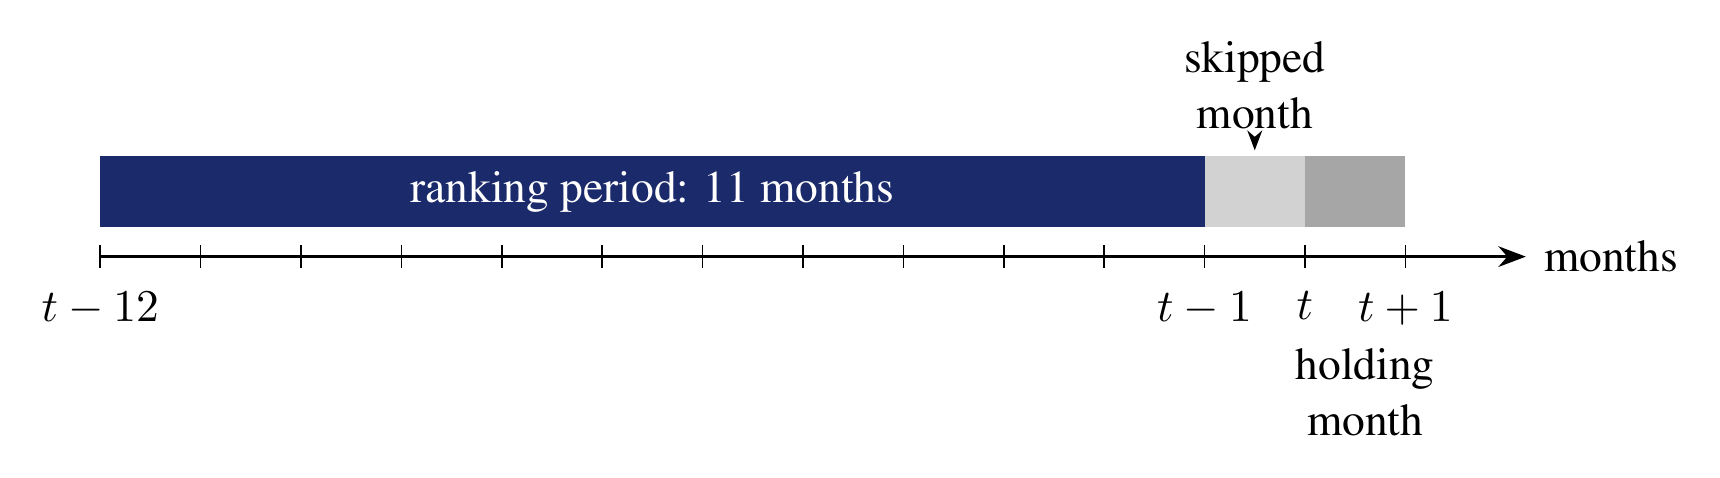
\includegraphics[width=0.9\linewidth]{images/fig09-1-signal.png}
\caption{The 12--1 momentum signal. Stocks are ranked on their return over the eleven months from $t-12$ to $t-1$; the most recent month is skipped; the portfolio is held for the month that follows.}
\label{fig:09-signal}
\end{figure}

\textbf{Cross-sectional momentum.} \textbf{Cross-sectional} or \textbf{relative} momentum ranks stocks against each other: buy the stocks with the highest past returns (\textbf{winners}) and sell those with the lowest (\textbf{losers}), regardless of whether the market as a whole rose or fell. Its long--short portfolio is \textbf{market-neutral} on average: over time its beta to the market is close to zero. The Fama--French momentum factor, often called \textbf{UMD} (up minus down) or Mom, is built this way, from six portfolios sorted on size and past return, in the same style as HML (Section~\ref{sec:08-how}).

\textbf{Time-series momentum.} \textbf{Time-series} or \textbf{absolute} momentum looks at each asset on its own: hold it long if its own past return is positive, short if negative. It is also called \textbf{trend following}, and it is what most \textbf{managed-futures funds}, funds that trade futures contracts across many markets, do. Unlike cross-sectional momentum it can be \textbf{net long} or \textbf{net short} the market, holding more long than short positions or the reverse, and it is usually applied across asset classes: stock indices, government bonds, currencies and commodities.

\textbf{Volatility scaling.} Many strategies size positions inversely to recent volatility, holding more when markets are calm and less when they are turbulent. If a position is scaled to
\begin{equation}
  w = \frac{\sigma^*}{\hat\sigma}
  \label{eq:09-volscale}
\end{equation}
where $\sigma^*$ is a target volatility and $\hat\sigma$ a forecast of the asset's volatility, its risk stays roughly constant over time. With a 12\% target and a forecast of 24\%, the position is halved; with a forecast of 8\%, it is one and a half times the base size. The forecast must use only data available before the position is set.

\textbf{Underreaction and overreaction.} \textbf{Behavioral finance} studies how investors' systematic errors affect prices. Two errors matter here.

\begin{itemize}
  \item \textbf{Underreaction}: investors adjust too slowly to news, because of conservatism or limited attention, so prices drift in the direction of the news for months.
  \item \textbf{Overreaction}: investors extrapolate a run of good or bad news too far, pushing prices past their fair value, which later reverses.
\end{itemize}

Momentum at horizons of a few months to a year fits underreaction or delayed overreaction; the long-run reversals documented by De Bondt and Thaler (1985) fit overreaction followed by correction.

\textbf{Beta that changes over time.} A long--short portfolio's market beta is the beta of its long side minus the beta of its short side. When the composition of the portfolio changes, so does its beta. After a market crash, the stocks that fell most, the losers, are typically high-beta stocks, so a momentum portfolio that is short them has a large negative beta. If the market then rebounds sharply, the portfolio loses heavily. This simple mechanism, explained in Section~\ref{sec:09-how}, accounts for momentum's worst months.

\textbf{Worked example.} A stock returned +40\% from twelve months ago to two months ago and $-5$\% last month. Its 12--1 momentum signal is +40\%, ignoring last month. If it ranks in the top 30\% of stocks on that signal, the momentum factor holds it in the winner portfolio for the coming month.

\textbf{Further reading.} Bodie, Kane and Marcus, \emph{Investments}, chapters on market efficiency and behavioral finance; Ilmanen, \emph{Expected Returns}, chapters on momentum and trend following; Ang, \emph{Asset Management}, chapter on factor strategies.

\section{How it works}
\label{sec:09-how}

\textbf{The strategy.} At the end of each month, rank stocks on their 12--1 past return. Buy the top group, sell the bottom group, hold for a month, and repeat. Because the ranking window shifts by one month at a time, ten of its eleven months carry over, and about a third of each side of the portfolio is replaced each month (Chapter 6). Jegadeesh and Titman (1993) studied many combinations of ranking and holding periods from three to twelve months; the 12--1 ranking with a one-month hold has become the standard.

\textbf{Why momentum might exist.} Three families of explanation compete.

\begin{itemize}
  \item \textbf{Underreaction.} Investors update slowly. Good news about a firm is only partly reflected in its price at first, and the rest arrives over the following months. Hong and Stein (1999) model news diffusing gradually through the investor population; Barberis, Shleifer and Vishny (1998) model investors who are too conservative in updating their beliefs.
  \item \textbf{Delayed overreaction.} Daniel, Hirshleifer and Subrahmanyam (1998) argue that overconfident investors, seeing their views confirmed by early price moves, push prices further than fundamentals justify, producing momentum in the medium term and reversal later.
  \item \textbf{Risk.} Momentum's crashes are themselves a candidate explanation: a strategy that loses heavily in rare, sharp market rebounds may earn a premium for bearing that risk. Rational models in which expected returns vary with firms' growth options have also been proposed, though none has become standard.
\end{itemize}

\textbf{Crashes and changing beta.} Momentum's market beta is not constant (Figure~\ref{fig:09-beta}). In a rising market, past winners are high-beta stocks and momentum has positive beta. After a market decline, past losers are the high-beta stocks and momentum is short them, giving it a strongly negative beta. Grundy and Martin (2001) noted this time variation; Daniel and Moskowitz (2016) showed that it explains momentum's crashes, which occur when markets rebound after a decline, and that their timing is partly predictable from the past market return and recent volatility.

\begin{figure}[htbp]
\centering
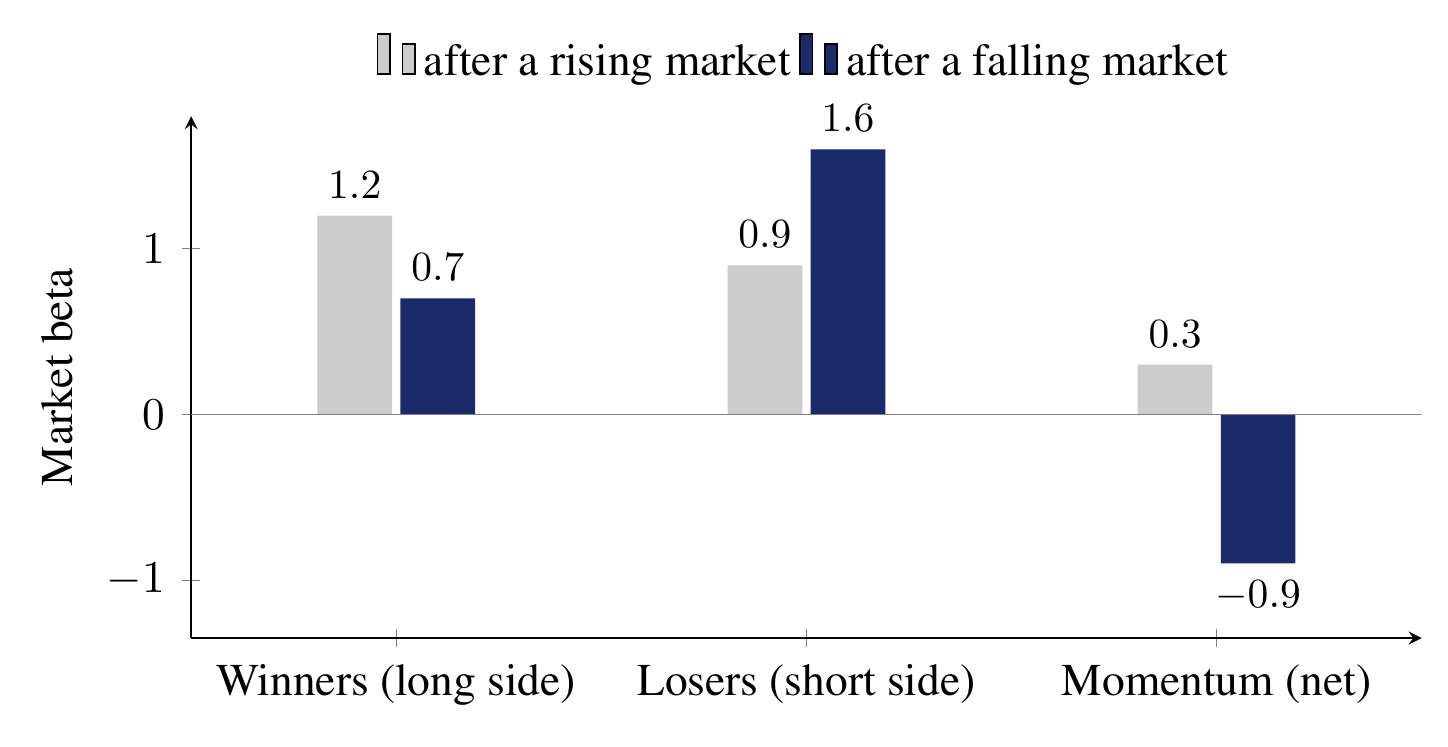
\includegraphics[width=0.85\linewidth]{images/fig09-2-beta.png}
\caption{Why momentum's beta flips (illustrative values). After a rising market the winners it holds are the high-beta stocks, so its net beta is positive. After a falling market the losers it sells short are the high-beta stocks, so its net beta turns strongly negative, and a sharp market rebound produces a large loss.}
\label{fig:09-beta}
\end{figure}

\textbf{Managing the crashes.} Because momentum's volatility rises sharply before and during crashes, scaling the position by forecast volatility, as in Equation~\eqref{eq:09-volscale}, cuts exposure when crashes are most likely. Barroso and Santa-Clara (2015) found that this nearly doubled momentum's Sharpe ratio and largely eliminated its crashes in U.S. data. Daniel and Moskowitz (2016) proposed a dynamic version that also uses a forecast of momentum's mean return.

\section{The claim}
\label{sec:09-claim}

Stated so that it can fail:

\begin{callout}
\textbf{Stocks with high returns over the past year continue to outperform stocks with low past returns over the following months, by enough to survive costs, in data beyond the samples that established the result, and with risks an investor can manage.}
\end{callout}

The final clause is what distinguishes this chapter's claim from a simple statement about average returns. A premium that is real on average but delivers losses of 50\% or more in a few months may be a premium few investors can collect. The tests follow:

\begin{itemize}
  \item \textbf{Time.} Is the premium present after Jegadeesh and Titman's 1965--1989 sample, and in every era?
  \item \textbf{Breadth.} Is it found in other countries and asset classes?
  \item \textbf{Costs.} Momentum trades far more than value. Does its premium exceed its costs?
  \item \textbf{Crashes.} How large are the crashes, can they be anticipated, and does managing them change the verdict?
\end{itemize}

\section{The original evidence}
\label{sec:09-evidence}

\textbf{Jegadeesh and Titman (1993)} sorted U.S. stocks from 1965 to 1989 on their past three- to twelve-month returns and found that buying winners and selling losers earned about 1\% a month, a result that could not be explained by market risk. They also found that part of the profit reversed after a year or more. \textbf{Jegadeesh and Titman (2001)} returned to the question with the years after their first paper and found that momentum continued to earn a similar premium out of sample, one of the earliest successful post-publication tests of an anomaly.

\textbf{Carhart (1997)} added a momentum factor to the Fama--French three-factor model to study mutual fund performance. The four-factor model became a standard benchmark, and Carhart's finding that much of the apparent persistence in fund returns was momentum exposure rather than skill was influential in its own right. Fama and French themselves did not include momentum in their models, while noting that their three factors could not explain it.

\textbf{Breadth.} Rouwenhorst (1998) found momentum in twelve European markets. Asness, Moskowitz and Pedersen (2013) found it in stocks across countries and in government bonds, currencies and commodity futures. Moskowitz, Ooi and Pedersen (2012) documented \textbf{time-series momentum} in 58 futures and forward contracts across four asset classes: an asset's own past twelve-month return predicted its return over the next month in almost every market studied. The notable exception is Japan, where Chui, Titman and Wei (2010) and others found cross-sectional momentum weak or absent.

\textbf{Crashes.} Daniel and Moskowitz (2016) documented that momentum's worst losses come in clusters after market declines, when the market rebounds. In the spring of 2009, as the market recovered from the financial crisis, past losers, many of them battered financial and cyclical stocks, rose far more than past winners. A similar episode occurred in 1932. The crashes were large enough that momentum's long-run return, though positive, came with negative skewness and extreme drawdowns. Barroso and Santa-Clara (2015) showed that scaling by forecast volatility removed much of this risk in U.S. data.

\section{Replication lab: Lab 9}
\label{sec:09-lab}

\begin{callout}
\textbf{Lab 9 at a glance.} \emph{The question:} has momentum earned a premium throughout the century of U.S. data, when do its crashes occur, and can volatility scaling make it a strategy an investor could hold? \emph{Data:} Kenneth French's library: the monthly and daily momentum factor from the 1920s, the market factor and risk-free rate, ten portfolios sorted on 12--2 past returns, and ten industry portfolios. Optionally, the Jensen--Kelly--Pedersen data for momentum in many countries. \emph{Code:} repository folder \texttt{ch09-momentum/}, with a guided notebook.
\end{callout}

\textbf{The setup.}

\begin{itemize}
  \item \textbf{Part A, replication.} Momentum's average return, t-statistic, Sharpe ratio, skewness, worst month and \textbf{maximum drawdown}, the largest fall from a previous peak, over the full sample, by decade, before and during the Jegadeesh--Titman sample, and after publication. The average returns of the ten momentum deciles show whether returns rise steadily from losers to winners.
  \item \textbf{Part B, crashes.} The ten worst months, with the market's return that month and over the previous two years. A regression of momentum on the market, with extra terms for \textbf{bear markets} (here, periods when the market's past 24-month return is negative) and for bear-market months in which the market rises, measures how momentum's beta changes.
  \item \textbf{Part C, volatility scaling.} Each month, momentum is scaled to a 12\% annual volatility target using the volatility of its daily returns over the previous six months. Its results are compared with raw momentum levered to the same average volatility, so the comparison is about timing, not leverage.
  \item \textbf{Part D, time-series momentum.} Each of ten industry portfolios and the market is held long or short according to the sign of its past twelve-month excess return, scaled to equal volatility. This is a narrow, equity-only version of Moskowitz, Ooi and Pedersen's test, and the lab says so.
  \item \textbf{Part E, costs.} Net returns at one-way costs of 20 and 50 basis points, using momentum's turnover of about 35\% a month.
\end{itemize}

\textbf{What readers will find.} Figure 9.3 marks the five worst months on a century-long chart of momentum's growth; Figure 9.5 shows that they cluster in the upper right of a scatter of momentum against the market during bear markets: when beaten-down markets rebound. Figure 9.6 compares raw and volatility-scaled momentum, with their drawdowns. The test of the claim is whether the premium is present in most decades and after publication, survives costs, and whether its crashes are manageable without hindsight.

\section{Stress tests}
\label{sec:09-stress}

\textbf{1. After publication.} Jegadeesh and Titman's paper appeared in 1993. Momentum's post-publication record is one of the longest out-of-sample tests of any anomaly, and Jegadeesh and Titman (2001) found it continued to work through the 1990s. The lab extends the test to the present, through the 2009 crash and the 2010s.

\textbf{2. Other countries and asset classes.} The international evidence is broad but not universal: momentum is strong in Europe and weak in Japan. The JKP data allow a country-by-country count, with Chapter 4's caution about how many significant results to expect by chance.

\textbf{3. Costs.} With turnover of about 35\% a month on each side, momentum pays four times that fraction of the one-way cost each month (Equation~\eqref{eq:06-net}). At 20 basis points, costs absorb roughly $4 \times 0.35 \times 0.20 \times 12 \approx 3$ percentage points of the annual premium; at 50 basis points, about 8. Novy-Marx and Velikov (2016) estimated momentum's costs at about 0.65\% a month and found it still earned a significant net premium, unlike higher-turnover strategies (Chapter 6). Volatility scaling adds trading when the weight changes; the lab charges for that too.

\textbf{4. Crashes and their predictability.} A crash that could be predicted only with hindsight is no help to an investor. The lab uses only information available at the start of each month: the past 24-month market return for the bear-market indicator, and past daily volatility for scaling. The test is whether those signals, set in advance, reduce the crashes.

\textbf{5. The volatility-scaling result itself.} A result that improves on a famous anomaly by adjusting it is itself a claim that can be overfit. Barroso and Santa-Clara chose a six-month window and a 12\% target; the lab lets readers change both, and an exercise asks how sensitive the improvement is. Chapter 11 returns to whether volatility timing works in general.

\section{Verdict}
\label{sec:09-verdict}

Based on the published evidence, to be confirmed by readers' runs of Lab 9 on data through 2025: \textbf{survives, with severe crash risk.}

\begin{center}
\small
\begin{tabularx}{0.9\linewidth}{@{}>{\raggedright\arraybackslash}p{0.22\linewidth}>{\raggedright\arraybackslash}X>{\raggedright\arraybackslash}p{0.25\linewidth}@{}}
\toprule
Test & Finding & Effect on the claim \\
\midrule
A century of U.S. data & A large average premium with a high t-statistic & Supports \\
After publication & Continued to earn a premium through the 1990s; weaker and more volatile since 2000, with the 2009 crash & Supports, weakened \\
Other countries and assets & Broad, with Japan the notable exception & Supports \\
Costs & Large, but smaller than the gross premium at institutional costs & Supports, with a smaller net premium \\
Crashes & Rare, severe and concentrated in market rebounds after declines & A serious qualification \\
Volatility scaling & Reduces crashes and raises the Sharpe ratio in the literature, using only past data & Supports manageability, but is itself a claim to test \\
\bottomrule
\end{tabularx}
\end{center}

Momentum is among the most robust anomalies in finance: it has survived publication, appears in most markets and asset classes, and covers its costs at institutional trading costs. Its crashes are the reason the verdict is not an unqualified survives: an investor holding raw momentum must be prepared to lose a large fraction of the strategy's value in a few months, at moments when the rest of the portfolio is recovering. The verdict is dated by the sample tested.

\section{What investors can use}
\label{sec:09-investors}

\textbf{Trend rules for asset allocation.} Time-series momentum applied across asset classes, the core of managed-futures funds, has historically tended to do well in prolonged market declines, when it turns short. That makes it a candidate \textbf{diversifier}, an addition that tends to do well when the rest of the portfolio does badly, for a stock-heavy portfolio. Its returns have been uneven, with long flat periods, and its fees are often high.

\textbf{Stock-picking momentum.} Cross-sectional momentum is best held as one component of a multi-factor portfolio. It is negatively correlated with value, so combining the two smooths returns (Asness, Moskowitz and Pedersen 2013). On its own, its crashes make it hard to hold.

\textbf{Manage the risk, not just the return.} Volatility scaling, or at least sizing a momentum allocation so that a 50\% loss in a few months would be survivable, is more important than any refinement of the signal.

\textbf{Questions to ask a momentum or trend-following manager:}

\begin{enumerate}
  \item How did the strategy perform from March to May 2009, and what would it do in a similar rebound?
  \item Is the position sized by volatility, and was that rule fixed before the backtest?
  \item What is the strategy's turnover, and what costs were assumed? How do they compare with your live trading costs?
  \item How much of the return comes from small, illiquid stocks?
  \item Over which periods has the strategy failed to make money, and for how long?
\end{enumerate}

\begin{callout}
\textbf{What Failed: holding raw momentum through the 2009 rebound.} By early 2009 momentum had performed well through the financial crisis: it was long defensive winners and short the collapsing financial and cyclical stocks. When the market turned in March 2009, the most beaten-down stocks rebounded hardest. Over the following months, momentum's loser portfolio rose far more than its winner portfolio, and the strategy lost much of a decade's gains in a few months (Daniel and Moskowitz 2016). Nothing about the crash was a mystery afterward: the strategy was short a portfolio of very high-beta stocks at the bottom of a bear market. The failure was in treating momentum's average return as the whole story, and in sizing positions as if the risk were constant. The claim that momentum's historical return could be harvested without managing its crash risk \textbf{fails}.
\end{callout}

\section{Open questions}
\label{sec:09-open}

\begin{itemize}
  \item \textbf{Can momentum crashes be forecast in real time?} The bear-market and volatility signals help in sample. How well do they work for an investor who adopts them today, and do they survive Chapter 4's multiple-testing corrections?
  \item \textbf{Why not Japan?} Cultural explanations, differences in investor behavior and differences in market structure have all been proposed for momentum's weakness in Japan; none is settled.
  \item \textbf{Risk or behavior?} If crashes are the risk that momentum's premium compensates, managing the crashes should reduce the premium. Does it?
  \item \textbf{Momentum in factors.} Ehsani and Linnainmaa (2022) argue that factor returns themselves have momentum. How does that relate to momentum in individual stocks?
\end{itemize}

\section*{Exercises}
\addcontentsline{toc}{section}{Exercises}

\subsection*{Conceptual (all readers)}

\begin{enumerate}
  \item Why does the standard momentum signal skip the most recent month? What would happen to the strategy's returns if it did not?
  \item Explain the difference between cross-sectional and time-series momentum. In a year when every stock rises, what does each strategy do?
  \item Explain, using betas, why momentum loses when a falling market rebounds sharply.
  \item Volatility scaling raised momentum's Sharpe ratio in the original study. List two reasons the improvement might be smaller for an investor who adopts it now.
\end{enumerate}

\subsection*{Lab extensions (technical readers)}

\begin{enumerate}
  \setcounter{enumi}{4}
  \item Re-run Part C with a weight cap of 1.5 and with targets of 8\% and 16\%. How sensitive is the improvement?
  \item Replace the 24-month bear-market indicator with a 12-month one. Does the crash regression change?
  \item Compute momentum's net Sharpe ratio after 2001 with a one-way cost of 10 basis points. Is momentum more implementable today?
  \item In Part D, change the look-back from 12 months to 3 and to 24. How does time-series momentum change?
  \item Using the JKP data, count the countries in which momentum has a t-statistic above 2. How many would you expect by chance?
  \item Combine momentum and value (Chapter 8) in a 50/50 portfolio. Compare its Sharpe ratio, skewness and worst drawdown with each strategy alone.
\end{enumerate}

\section*{References}
\addcontentsline{toc}{section}{References}

\begin{itemize}
  \item Asness, C. S., Moskowitz, T. J. and Pedersen, L. H. (2013). Value and Momentum Everywhere. \emph{Journal of Finance} 68(3): 929--985.
  \item Barberis, N., Shleifer, A. and Vishny, R. (1998). A Model of Investor Sentiment. \emph{Journal of Financial Economics} 49(3): 307--343.
  \item Barroso, P. and Santa-Clara, P. (2015). Momentum Has Its Moments. \emph{Journal of Financial Economics} 116(1): 111--120.
  \item Carhart, M. M. (1997). On Persistence in Mutual Fund Performance. \emph{Journal of Finance} 52(1): 57--82.
  \item Chui, A. C. W., Titman, S. and Wei, K. C. J. (2010). Individualism and Momentum around the World. \emph{Journal of Finance} 65(1): 361--392.
  \item Daniel, K., Hirshleifer, D. and Subrahmanyam, A. (1998). Investor Psychology and Security Market Under- and Overreactions. \emph{Journal of Finance} 53(6): 1839--1885.
  \item Daniel, K. and Moskowitz, T. J. (2016). Momentum Crashes. \emph{Journal of Financial Economics} 122(2): 221--247.
  \item De Bondt, W. F. M. and Thaler, R. (1985). Does the Stock Market Overreact? \emph{Journal of Finance} 40(3): 793--805.
  \item Ehsani, S. and Linnainmaa, J. T. (2022). Factor Momentum and the Momentum Factor. \emph{Journal of Finance} 77(3): 1877--1919.
  \item Grundy, B. D. and Martin, J. S. (2001). Understanding the Nature of the Risks and the Source of the Rewards to Momentum Investing. \emph{Review of Financial Studies} 14(1): 29--78.
  \item Hong, H. and Stein, J. C. (1999). A Unified Theory of Underreaction, Momentum Trading, and Overreaction in Asset Markets. \emph{Journal of Finance} 54(6): 2143--2184.
  \item Jegadeesh, N. and Titman, S. (1993). Returns to Buying Winners and Selling Losers: Implications for Stock Market Efficiency. \emph{Journal of Finance} 48(1): 65--91.
  \item Jegadeesh, N. and Titman, S. (2001). Profitability of Momentum Strategies: An Evaluation of Alternative Explanations. \emph{Journal of Finance} 56(2): 699--720.
  \item Moskowitz, T. J., Ooi, Y. H. and Pedersen, L. H. (2012). Time Series Momentum. \emph{Journal of Financial Economics} 104(2): 228--250.
  \item Novy-Marx, R. and Velikov, M. (2016). A Taxonomy of Anomalies and Their Trading Costs. \emph{Review of Financial Studies} 29(1): 104--147.
  \item Rouwenhorst, K. G. (1998). International Momentum Strategies. \emph{Journal of Finance} 53(1): 267--284.
\end{itemize}

\textbf{Data:} Kenneth R. French Data Library, \url{https://mba.tuck.dartmouth.edu/pages/faculty/ken.french/data_library.html}. Jensen--Kelly--Pedersen global factor data, \url{https://jkpfactors.com}.

% Chapter 10 -- Claim: Most Anomalies Are False
% Requires: amsmath, amssymb, booktabs, array, tabularx, graphicx, tcolorbox (breakable, skins), hyperref or url.
% Defines the callout box only if the preamble has not.
\providecolor{fenavy}{HTML}{1B2A6B}
\providecolor{feshade}{HTML}{F3F5FA}
\makeatletter
\@ifundefined{callout}{%
  \newtcolorbox{callout}{breakable, enhanced,
    colback=white, colframe=gray!70, boxrule=0.5pt, arc=1mm,
    borderline west={2.5pt}{0pt}{gray!70},
    left=8pt, right=8pt, top=4pt, bottom=4pt}%
}{}
\makeatother

\chapter{Claim: Most Anomalies Are False}
\label{ch:10}

Chapters 8 and 9 examined two famous anomalies in depth. This chapter steps back to the whole population. Academic finance has published hundreds of variables said to predict the cross-section of stock returns. If Chapter 4's arithmetic applies, many of them should be false discoveries. In 2020 a widely cited study reported that most of them fail to replicate; in 2023 an equally careful study concluded that most of them do replicate.

Both studies were done by respected researchers using largely the same data. They reached opposite conclusions because they asked slightly different questions and applied different standards. That makes this chapter's claim unusual: the verdict depends less on the data than on the rules of evidence, and the reader is asked to choose those rules and defend them.

The chapter presents the case for the prosecution and the case for the defense, measures what happens to published predictors after their samples end and after they are published, and gives readers a lab in which they can apply each side's standards to the same data.

By the end of the chapter you will be able to:

\begin{itemize}
  \item explain the three forms of market efficiency and the joint-hypothesis problem;
  \item define an anomaly, and distinguish reproduction, pure replication, scientific replication and out-of-sample replication;
  \item explain how publication bias inflates published results, and how empirical Bayes shrinkage corrects noisy estimates;
  \item list the design choices that can change whether an anomaly replicates;
  \item set out the prosecution's and the defense's cases, and explain why they reach opposite verdicts from similar data;
  \item separate post-publication decay due to selection from decay due to investors' learning;
  \item write and defend your own verdict, stating the standard of evidence you apply.
\end{itemize}

\section{Foundations: market efficiency, anomalies and replication}
\label{sec:10-foundations}

\textbf{The efficient market hypothesis.} A market is \textbf{informationally efficient} if prices fully reflect available information, so that no investor can earn returns above those justified by risk using that information. Fama (1970) distinguished three forms by the information involved: \textbf{weak} (past prices), \textbf{semi-strong} (all public information) and \textbf{strong} (all information, including private). Efficiency does not mean prices are always right; it means mispricings cannot be predicted and exploited systematically after costs (Section~\ref{sec:01-efficient-markets}).

\textbf{The joint-hypothesis problem.} Any test of efficiency needs a model of what returns \emph{should} be, such as the CAPM. If a strategy earns more than the model predicts, either the market is inefficient or the model is wrong. The two cannot be separated (Fama 1970). This is why the same evidence can be read as mispricing by one researcher and as compensation for an unmodeled risk by another.

\textbf{Anomalies.} An \textbf{anomaly} is a pattern in returns that a benchmark asset pricing model cannot explain: a characteristic, such as a valuation ratio or past return, that predicts future returns after adjusting for the model's risk factors. Anomalies are usually documented with portfolio sorts and long--short returns (Section~\ref{sec:08-foundations}) and judged by the t-statistic of the average return or alpha.

\textbf{Replication, reproduction and robustness.} Terms are used loosely, but a useful distinction is:

\begin{itemize}
  \item \textbf{Reproduction}: the same data and code give the same numbers. It checks for errors.
  \item \textbf{Pure replication}: the same method on the same kind of data, perhaps rebuilt independently, gives the same result. It checks that the finding is not an artifact of one implementation.
  \item \textbf{Scientific replication} or \textbf{robustness}: different but reasonable choices of method, sample or market give a similar result. It checks that the finding is about the world, not about the choices.
  \item \textbf{Out-of-sample replication}: the result holds in data not used to find it, such as later years or other countries.
\end{itemize}

The two sides of this chapter's debate differ largely in which of these they demand.

\textbf{Publication bias.} Journals are more likely to publish significant results. If only strong in-sample results are published, the published estimates are biased upward even if every individual study was done honestly: the published set is selected for luck as well as truth. Part E of this chapter's lab measures how large this effect can be.

\textbf{Shrinkage.} When many noisy estimates are made at once, a better estimate of each true value pulls it toward the average of all of them, more for noisier estimates and less for precise ones. A very high estimate is more likely to be partly luck than a moderate one, so pulling it back improves it on average. This idea, from \textbf{empirical Bayes} statistics (Efron and Morris 1975), in which the data themselves supply the average toward which estimates are pulled, is the basis of the defense's methodology.

\textbf{Worked example.} One hundred honest researchers each test a different trading signal with no true predictive power. By chance, about five will find t-statistics beyond $\pm 1.96$, and those five publish (Figure~\ref{fig:10-pubbias}). Every published paper reports a significant result; none is real. A reader who saw only the journals would find a literature with a 100\% success rate.

\begin{figure}[htbp]
\centering
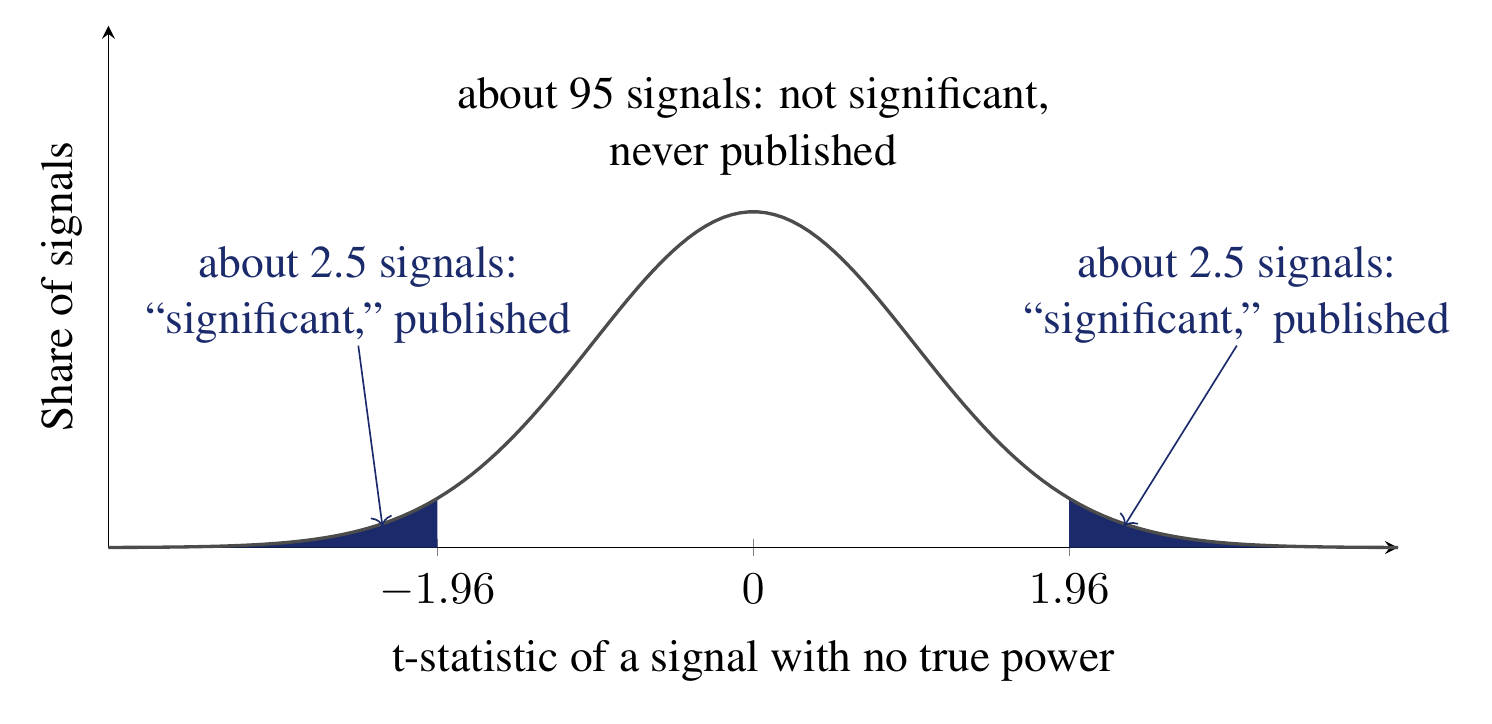
\includegraphics[width=0.85\linewidth]{images/fig10-1-publication-bias.png}
\caption{Publication bias. One hundred signals with no true power produce t-statistics spread around zero. Only the few in the shaded tails, about 2.5 on each side, look significant and get published. The published record shows only the tails.}
\label{fig:10-pubbias}
\end{figure}

\textbf{Further reading.} Bodie, Kane and Marcus, \emph{Investments}, chapters on market efficiency and behavioral finance; Bali, Engle and Murray, \emph{Empirical Asset Pricing}, on portfolio sorts and anomalies; Efron and Hastie, \emph{Computer Age Statistical Inference}, chapters on empirical Bayes and large-scale hypothesis testing.

\section{How it works: the factor zoo and how replications are designed}
\label{sec:10-how}

\textbf{The zoo.} Chapter 4 introduced Cochrane's ``zoo of new factors'' and Harvey, Liu and Zhu's (2016) count of 316 factors published in leading journals. Since then, two open data projects have made it possible to rebuild most of them:

\begin{itemize}
  \item Chen and Zimmermann's \textbf{Open Source Asset Pricing} (2022) replicates more than 200 cross-sectional predictors from the original papers' descriptions and publishes their portfolio returns and code.
  \item Jensen, Kelly and Pedersen (2023) built a \textbf{global factor database} of 153 factors across 93 countries, with harmonized definitions, meaning each factor is built the same way in every country.
\end{itemize}

\textbf{Design choices in a replication.} A replication of an anomaly must make many choices, each defensible, that can change the result:

\begin{center}
\small
\begin{tabularx}{0.9\linewidth}{@{}>{\raggedright\arraybackslash}p{0.17\linewidth}>{\raggedright\arraybackslash}X>{\raggedright\arraybackslash}p{0.34\linewidth}@{}}
\toprule
Choice & Options & Why it matters \\
\midrule
Universe & All stocks, or excluding micro-caps (for example below the NYSE 20th size percentile) & Many anomalies are concentrated in tiny stocks that are costly to trade and hold little value \\
Weighting & Equal-weighted or value-weighted portfolios & Equal weighting gives micro-caps large influence \\
Breakpoints & Deciles, quintiles or terciles; NYSE or all-stock breakpoints & Extreme portfolios magnify signals and noise \\
Sample & The original paper's sample, or the longest available & Later years are out of sample \\
Significance hurdle & $t > 1.96$, $t > 3$, a false-discovery-rate rule, or a Bayesian posterior & Determines what counts as a success \\
Benchmark & Raw returns, CAPM alpha, or alpha against a multifactor model & A factor explained by others may be real but redundant \\
\bottomrule
\end{tabularx}
\end{center}

\textbf{NYSE breakpoints} set the cut-offs between groups using only stocks listed on the New York Stock Exchange, which are larger on average, so the many tiny Nasdaq stocks do not crowd the extreme portfolios. A \textbf{Bayesian posterior} is the probability of a hypothesis after combining a prior belief with the data.

\textbf{Pure and scientific replication again.} A replication that copies the original method tests whether the paper's numbers can be reproduced. One that changes the universe, weighting or hurdle tests whether the finding is robust. Both are valuable, but they answer different questions, and the debate in this chapter turns partly on that difference.

\section{The claim}
\label{sec:10-claim}

Stated so that it can fail:

\begin{callout}
\textbf{Most published cross-sectional return predictors do not reflect a real, persistent relationship: they fail to replicate under reasonable standards, or their returns disappear outside the sample in which they were found.}
\end{callout}

``Reasonable standards'' is where the debate lies. The claim can be tested in three ways:

\begin{itemize}
  \item \textbf{Replication within the original sample.} Do the predictors' long--short returns clear a significance hurdle when rebuilt independently? Which hurdle, and with which portfolio construction?
  \item \textbf{Out of sample.} Do returns persist after the original sample ends and after publication?
  \item \textbf{Statistically corrected.} After accounting for the number of predictors tested and for publication bias, what share have a high probability of a positive true return?
\end{itemize}

\section{The prosecution}
\label{sec:10-prosecution}

\textbf{Harvey, Liu and Zhu (2016)} argued from statistics: with hundreds of factors tested, and many more tested but never published, the conventional $t > 2$ hurdle lets through too many false discoveries. Adjusting for the number of tests, they proposed that a new factor should clear a t-statistic of about 3, and concluded that many published factors were likely false.

\textbf{Hou, Xue and Zhang (2020)} argued from replication. They rebuilt 452 anomalies with a common method designed to limit the influence of micro-caps: NYSE breakpoints and value-weighted returns. Under that method, 65\% of the anomalies could not clear the single-test hurdle of an absolute t-statistic of 1.96, and raising the hurdle to 2.78 to allow for multiple testing raised the failure rate to 82\%. Anomalies based on \textbf{trading frictions}, the costs and obstacles of trading, such as illiquidity and idiosyncratic risk measures, failed most often, 96\% of them. \textbf{Idiosyncratic risk} is the part of a stock's volatility not explained by the market or other factors. Their conclusion: most anomalies are either false or confined to micro-caps that are too small and costly to matter.

The prosecution's case rests on two premises: that the right hurdle is high because many tests have been run, and that the right portfolio construction gives little weight to the smallest stocks.

\section{The defense}
\label{sec:10-defense}

\textbf{Jensen, Kelly and Pedersen (2023)} argued that the replication crisis was overstated. Using a Bayesian model of factor replication, they found that:

\begin{itemize}
  \item most factors can be replicated;
  \item they cluster into 13 themes, most of which are significant parts of the optimal portfolio;
  \item they work out of sample in a large new data set covering 93 countries;
  \item the evidence is strengthened rather than weakened by the large number of factors, because related factors corroborate one another.
\end{itemize}

Their approach treats each factor's alpha as a draw from a common distribution and shrinks noisy estimates toward the average of related factors, rather than judging each one in isolation against a fixed hurdle.

\textbf{Chen and Zimmermann (2022)} found that the predictors whose original papers reported clear statistical evidence almost all reproduce with the original methods. \textbf{Chen and Zimmermann (2020)} estimated publication bias directly across 156 published predictors and concluded that bias-adjusted returns are only about 12\% smaller than in-sample returns, and that for predictors that survive journal review, a t-statistic hurdle of about 1.8 is enough to control for multiple testing. \textbf{Chen (2021)} argued that the sheer size of published t-statistics is hard to explain by \textbf{p-hacking}, trying analyses until one crosses the significance line, alone.

The defense's case rests on different premises: that the question is whether the original findings are real, not whether they survive a construction that de-emphasizes small stocks, and that evidence should be pooled across related factors rather than judged one test at a time.

\section{Post-publication decay}
\label{sec:10-decay}

Whatever the replication standard, out-of-sample performance is a separate question. \textbf{McLean and Pontiff (2016)} followed 97 predictors after their original samples ended and after publication. Portfolio returns were 26\% lower out of sample and 58\% lower after publication (Figure~\ref{fig:10-decay}). They interpreted the first figure as an upper bound on the effect of data mining, since nothing changed in the world when a sample ended except that researchers stopped looking, and attributed the further decline after publication to investors trading on the published results.

\begin{figure}[htbp]
\centering
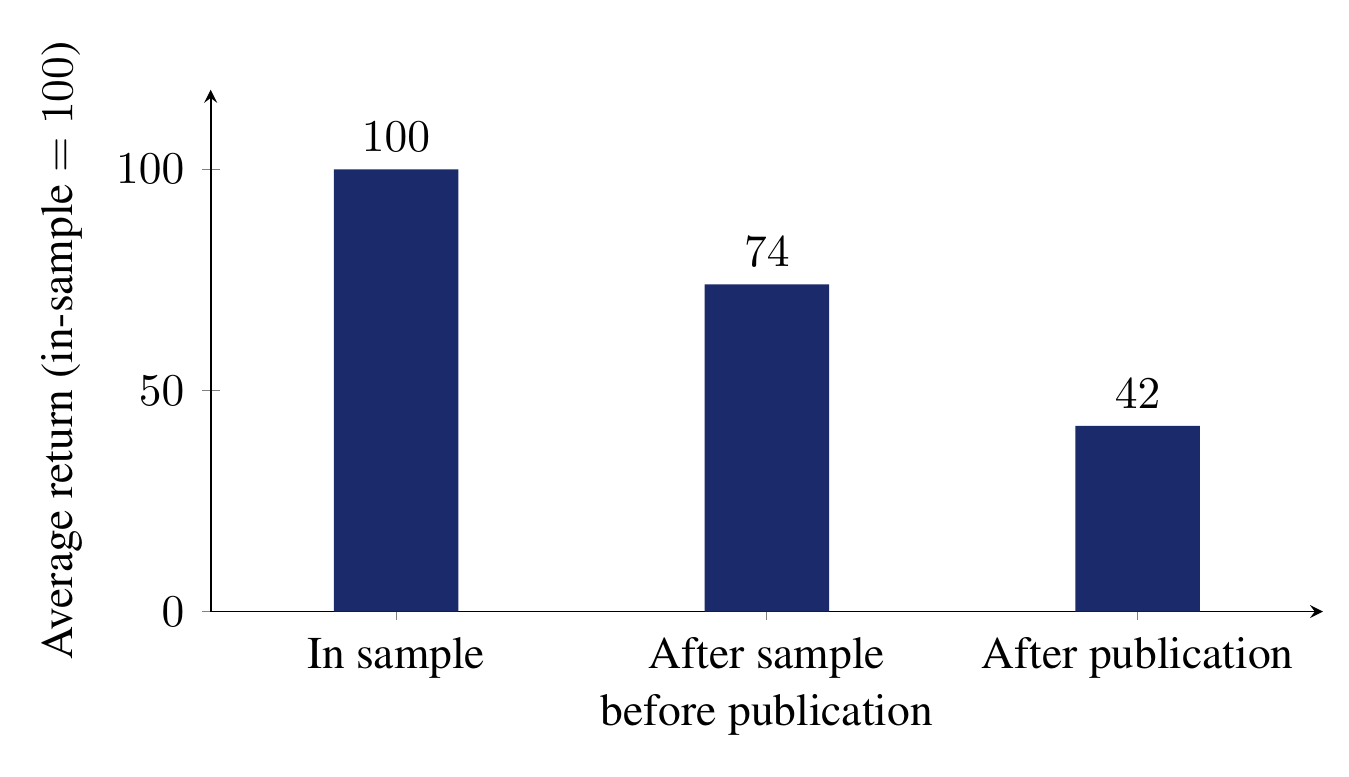
\includegraphics[width=0.75\linewidth]{images/fig10-2-decay.png}
\caption{Post-publication decay in McLean and Pontiff (2016). With in-sample returns set to 100, the average predictor earned 74 between the end of its original sample and publication, and 42 after publication.}
\label{fig:10-decay}
\end{figure}

The two readings matter for the claim. If most of the decline happens when the sample ends, the original results were inflated by selection: a sign of data mining. If most happens after publication, the results were real but have been arbitraged away by investors: a sign of learning, which is consistent with the original finding having been true. McLean and Pontiff's numbers suggest both forces matter, with the publication effect the larger.

This chapter's lab adds a check the original study could not make: a simulated literature in which the truth is known. If only significant results are published, returns appear to fall after the sample ends even when nothing changes. The size of that purely statistical decline is a benchmark for how much of the observed decay is selection.

\section{Replication lab: Lab 10}
\label{sec:10-lab}

\begin{callout}
\textbf{Lab 10 at a glance.} \emph{The question:} applying each side's standards to the same data, what share of published predictors survive, and how much of their return remains after their samples end and after publication? \emph{Data:} Open Source Asset Pricing: monthly long--short returns for more than 200 predictors as constructed in the original papers, and the signal documentation giving each paper's sample period and publication year. Optionally, a second construction of the same signals, value-weighted or excluding micro-caps, for the methodology comparison. \emph{Code:} repository folder \texttt{ch10-anomalies/}, with a guided notebook.
\end{callout}

\textbf{The setup.}

\begin{itemize}
  \item \textbf{Part A, replication.} Each predictor's t-statistic over its own original sample. The share clearing $t > 1.96$, $t > 3$, and a Benjamini--Hochberg false-discovery-rate test (Chapter 4).
  \item \textbf{Part B, decay.} Average returns in-sample, after the sample ended but before publication, and after publication. A \textbf{pooled regression}, which combines all predictors into one regression in the style of McLean and Pontiff, measures the proportional decline in each period with errors clustered by month (Section~\ref{sec:03-se}).
  \item \textbf{Part C, methodology.} The same statistics for an alternative construction, if supplied. This is the core of the disagreement between Hou, Xue and Zhang and the defense.
  \item \textbf{Part D, shrinkage.} An empirical Bayes estimate of each predictor's true mean, pulled toward the average in proportion to its noise; the share with more than 95\% probability of a positive true mean; and whether shrunk estimates predict post-publication returns better than raw ones.
  \item \textbf{Part E, known truth.} A simulated literature in which only signals with in-sample $t > 2$ are published, run with no true decay and with a 30\% decay after publication.
\end{itemize}

\textbf{What readers will find.} The simulation alone delivers one of the chapter's central lessons. When the lab's simulated literature was run with \textbf{no} true change after publication, the pooled regression still measured returns about 45\% lower after the samples ended and about 54\% lower after publication, purely because publication selected lucky in-sample results. With a true 30\% post-publication decay added, the measured post-publication decline rose to about 68\%. Readers who run the lab on the real data can compare McLean and Pontiff's figures, and their own, with this benchmark.

\section{Why the two sides disagree}
\label{sec:10-why}

The prosecution and the defense agree on most facts. They disagree on four choices.

\begin{center}
\small
\begin{tabularx}{0.9\linewidth}{@{}>{\raggedright\arraybackslash}p{0.17\linewidth}>{\raggedright\arraybackslash}X>{\raggedright\arraybackslash}X@{}}
\toprule
Choice & Prosecution (Hou, Xue and Zhang; Harvey, Liu and Zhu) & Defense (Jensen, Kelly and Pedersen; Chen and Zimmermann) \\
\midrule
Which stocks count & De-emphasize micro-caps: NYSE breakpoints, value weights & Replicate the original construction; micro-caps are part of the market \\
Hurdle & High: $t$ of about 3 or 2.78, for multiple testing & Lower, or a Bayesian posterior; multiple-testing corrections for published factors need not be severe \\
Unit of evidence & Each factor judged on its own & Related factors pooled; corroboration strengthens the evidence \\
Kind of replication & Scientific: does it survive reasonable alternative choices? & Pure: are the original findings reproducible and real? \\
\bottomrule
\end{tabularx}
\end{center}

Neither side is wrong on its own terms. A factor that appears only among micro-caps may be real and still irrelevant to an investor who cannot trade micro-caps. A factor that fails a $t > 3$ hurdle may be real and simply estimated with noise. A Bayesian estimate that pools related factors is more efficient if the pooling assumptions are right and misleading if a whole theme was mined together.

The practical lesson is that ``does this anomaly replicate?'' is not a well-posed question until the purpose is stated. For understanding how markets price risk, pure replication and pooled evidence are appropriate. For deciding what to invest in, value-weighted, liquid-universe, out-of-sample, after-cost evidence is what matters.

\section{Verdict: a split decision}
\label{sec:10-verdict}

This chapter's verdict is deliberately left to the reader, with the evidence summarized:

\begin{center}
\small
\begin{tabularx}{0.9\linewidth}{@{}>{\raggedright\arraybackslash}p{0.25\linewidth}>{\raggedright\arraybackslash}X>{\raggedright\arraybackslash}p{0.22\linewidth}@{}}
\toprule
Standard & What the evidence suggests & Verdict on ``most anomalies are false'' \\
\midrule
Original construction, conventional hurdle & Most published predictors reproduce & Fails \\
Micro-caps de-emphasized, value-weighted & Most fail to clear $t = 1.96$ (Hou, Xue and Zhang) & Survives \\
Bayesian pooling across related factors and countries & Most replicate and work out of sample (Jensen, Kelly and Pedersen) & Fails \\
Out of sample, after publication & Returns about half their in-sample level, part of it selection (McLean and Pontiff; Part E) & Weakens the anomalies, without making most false \\
After costs, for an investor & Little expected return remains for the average anomaly (Chen and Velikov 2023; Chapter 6) & Survives, in practice \\
\bottomrule
\end{tabularx}
\end{center}

A defensible summary: \textbf{most published anomalies are not pure statistical flukes, but most are smaller than reported, concentrated in small stocks, partly arbitraged away, and not profitable to trade after costs.} Whether that makes them ``false'' depends on whether the question is scientific or practical. Readers should write their own verdict, stating the standard they apply and why, and date it with the sample they tested.

\section{What investors can use}
\label{sec:10-investors}

\textbf{A checklist for judging any new factor fund or signal:}

\begin{enumerate}
  \item \textbf{Is the original evidence strong?} Ask for the t-statistic in the original study and whether it clears about 3.
  \item \textbf{Does it hold among large, liquid stocks, value-weighted?} If the effect lives in micro-caps, it is unlikely to be investable at scale.
  \item \textbf{What happened after publication?} Ask for returns from the paper's publication date forward. Expect roughly half the backtest at best.
  \item \textbf{Does it belong to a theme that works?} A signal related to established themes such as value, momentum, profitability or low risk has corroborating evidence; an isolated signal has none.
  \item \textbf{What survives costs?} Ask for turnover and net returns at realistic costs (Chapter 6).
  \item \textbf{How many signals did the provider test before choosing this one?} Apply Chapter 4's corrections to the answer.
\end{enumerate}

\begin{callout}
\textbf{What Failed: the trading-frictions anomalies.} A family of anomalies based on liquidity, idiosyncratic volatility and other trading frictions looked strong in the papers that introduced them. In Hou, Xue and Zhang's replication, 96\% of the anomalies in this category failed to clear a t-statistic of 1.96 once micro-caps were de-emphasized with NYSE breakpoints and value weights. Their returns had come mostly from the smallest, least liquid stocks, exactly where costs and frictions are largest. The claim that frictions-based anomalies offer returns an investor can capture \textbf{fails}; whether they reveal something real about how illiquid stocks are priced is a separate and open question.
\end{callout}

\section{Open questions}
\label{sec:10-open}

\begin{itemize}
  \item \textbf{What replication standard should the field adopt?} Should journals require value-weighted, micro-cap-robust results, pre-registered hurdles, or Bayesian posteriors?
  \item \textbf{How many signals were tested but never published?} The unknown size of this \textbf{file drawer}, the studies left unpublished, limits every correction for multiple testing.
  \item \textbf{Is post-publication decay learning or selection?} Part E's benchmark separates the two in simulation; doing so convincingly in real data remains open.
  \item \textbf{Do anomalies reflect risk or mispricing?} Their decay after publication favors mispricing for many; their persistence across countries favors something more durable for a few themes.
\end{itemize}

\section*{Exercises}
\addcontentsline{toc}{section}{Exercises}

\subsection*{Conceptual (all readers)}

\begin{enumerate}
  \item Explain the joint-hypothesis problem. Why can an anomaly never by itself prove that markets are inefficient?
  \item Distinguish pure replication from scientific replication. Which does Hou, Xue and Zhang's study perform, and which does Chen and Zimmermann's?
  \item Explain why a literature that publishes only significant results will show declining returns out of sample even if every published effect were partly real.
  \item Why might pooling related factors strengthen the evidence for each? When could pooling mislead?
\end{enumerate}

\subsection*{Lab extensions (technical readers)}

\begin{enumerate}
  \setcounter{enumi}{4}
  \item Run Part C with the micro-caps-excluded construction. How many signals drop below $t = 1.96$?
  \item Restrict the sample to signals published after 2000. Is post-publication decay larger or smaller than for older signals?
  \item In Part E, raise the publication threshold from $t > 2$ to $t > 3$. How does the apparent decay from selection change?
  \item In Part D, compare the shrunk estimates with post-publication returns for the 20 signals with the highest in-sample t-statistics. Which estimate predicts better?
  \item Estimate a \textbf{mixture prior} in which a share of signals have exactly zero true mean and the rest are normal. What share of zeros do the data imply?
  \item Write a two-page verdict on the chapter's claim, stating your standard of evidence and defending it against the other side.
\end{enumerate}

\section*{References}
\addcontentsline{toc}{section}{References}

\begin{itemize}
  \item Chen, A. Y. (2021). The Limits of p-Hacking: Some Thought Experiments. \emph{Journal of Finance} 76(5): 2447--2480.
  \item Chen, A. Y. and Velikov, M. (2023). Zeroing In on the Expected Returns of Anomalies. \emph{Journal of Financial and Quantitative Analysis} 58(3): 968--1004.
  \item Chen, A. Y. and Zimmermann, T. (2020). Publication Bias and the Cross-Section of Stock Returns. \emph{Review of Asset Pricing Studies} 10(2): 249--289.
  \item Chen, A. Y. and Zimmermann, T. (2022). Open Source Cross-Sectional Asset Pricing. \emph{Critical Finance Review} 11(2): 207--264.
  \item Efron, B. and Morris, C. (1975). Data Analysis Using Stein's Estimator and Its Generalizations. \emph{Journal of the American Statistical Association} 70(350): 311--319.
  \item Fama, E. F. (1970). Efficient Capital Markets: A Review of Theory and Empirical Work. \emph{Journal of Finance} 25(2): 383--417.
  \item Harvey, C. R., Liu, Y. and Zhu, H. (2016). \ldots and the Cross-Section of Expected Returns. \emph{Review of Financial Studies} 29(1): 5--68.
  \item Hou, K., Xue, C. and Zhang, L. (2020). Replicating Anomalies. \emph{Review of Financial Studies} 33(5): 2019--2133.
  \item Jensen, T. I., Kelly, B. and Pedersen, L. H. (2023). Is There a Replication Crisis in Finance? \emph{Journal of Finance} 78(5): 2465--2518.
  \item McLean, R. D. and Pontiff, J. (2016). Does Academic Research Destroy Stock Return Predictability? \emph{Journal of Finance} 71(1): 5--32.
\end{itemize}

\textbf{Data:} Open Source Asset Pricing, \url{https://www.openassetpricing.com}. Jensen--Kelly--Pedersen global factor data, \url{https://jkpfactors.com}.

\clearpage
\addcontentsline{toc}{chapter}{PART II: Deep Learning for Anomaly Detection}
\newpage

\vspace*{\fill}


\Large
\noindent\textbf{PART II: Deep Learning for Anomaly Detection}
\normalsize
\vspace*{3cm}


Part II introduces the foundations of deep learning for anomaly detection. While the earlier chapters focused primarily on classical machine learning and statistical approaches, this section explores how neural networks learn complex representations from data and how these representations can be leveraged to detect anomalies. Readers will develop a practical understanding of deep learning concepts, training procedures, image data processing, and representation learning before applying these ideas to deep-learning-based anomaly detection models.

\vspace*{0.5cm}

Chapter \ref{ch11}: Foundations of Deep Learning

Chapter \ref{ch12}: Training Deep Neural Networks

Chapter \ref{ch13}: Deep Learning for Image Data

Chapter \ref{ch14}: Autoencoders

Chapter \ref{ch15}: Variational Autoencoders (VAE)

\vspace*{\fill}


\clearpage
% Chapter 11 -- Claim: Volatility Is Predictable
% Requires: amsmath, amssymb, booktabs, array, tabularx, graphicx, tcolorbox (breakable, skins), hyperref or url.
% Defines the callout box only if the preamble has not.
\providecolor{fenavy}{HTML}{1B2A6B}
\providecolor{feshade}{HTML}{F3F5FA}
\makeatletter
\@ifundefined{callout}{%
  \newtcolorbox{callout}{breakable, enhanced,
    colback=white, colframe=gray!70, boxrule=0.5pt, arc=1mm,
    borderline west={2.5pt}{0pt}{gray!70},
    left=8pt, right=8pt, top=4pt, bottom=4pt}%
}{}
\makeatother

\chapter{Claim: Volatility Is Predictable}
\label{ch:11}

Chapters 7 to 10 asked whether anything forecasts the \emph{level} of returns, and the answers were mostly modest. This chapter asks about their \emph{size}. On that question the evidence is strong. A quiet day in the market tends to follow another quiet day, and a violent day tends to follow another violent one. The 1987 crash, the autumn of 2008 and March 2020 each arrived as a run of violent days, not a single one.

This is the most robust claim in the book, and it carries a lot of weight. Option prices, risk limits, Value at Risk (Chapter 13), margin requirements and the volatility-targeting funds that now manage hundreds of billions of dollars all assume that volatility can be forecast. So the questions here are less \emph{whether} than \emph{how well}, \emph{at what horizon}, and \emph{by which model}. A further question is whether an investor can turn the forecasts into better returns, and the evidence on that is much weaker.

By the end of the chapter you will be able to:

\begin{itemize}
  \item annualize a daily volatility and explain why models work in variance;
  \item compute historical, EWMA and GARCH volatility forecasts, the long-run variance and the half-life of a shock;
  \item explain realized variance, the HAR model, implied volatility, the VIX and the variance risk premium;
  \item state the claim that volatility is predictable in a form that can fail, and summarize the evidence for it;
  \item evaluate volatility forecasts with robust loss functions such as QLIKE, and with Mincer--Zarnowitz and Diebold--Mariano tests;
  \item judge whether volatility timing improves an investor's returns once forecasts are made in real time and costs and leverage limits apply.
\end{itemize}

\section{Foundations: measuring and modelling volatility}
\label{sec:11-foundations}

\textbf{Volatility and variance.} \textbf{Volatility} is the standard deviation of returns over a period. Practitioners quote it \emph{annualized}: a daily standard deviation $\sigma_d$ becomes $\sigma_d\sqrt{252}$, since there are about 252 trading days in a year, so a 1\% daily volatility is about 16\% a year. The square root assumes returns are uncorrelated from day to day, which Chapter 3 showed is close to true (Section~\ref{sec:03-facts}). \textbf{Variance} is volatility squared. Most models work in variance, because variances of uncorrelated returns add: the variance over the next $h$ days is the sum of the daily variances.

\textbf{Historical volatility} is the sample standard deviation over a past window, such as the last 22 trading days (about one month). It weights every day in the window equally and drops days abruptly when they leave it. Because daily mean returns are tiny compared with daily volatility, practitioners usually set the mean to zero and estimate variance as the average squared return.

\textbf{EWMA} (exponentially weighted moving average), popularized by J.P. Morgan's RiskMetrics in 1994, weights recent days more heavily:
\begin{equation}
  \sigma^2_t = \lambda\,\sigma^2_{t-1} + (1 - \lambda)\,r^2_{t-1}
  \label{eq:11-ewma}
\end{equation}
RiskMetrics set $\lambda = 0.94$ for daily data. Yesterday's squared return gets weight 6\%, the day before $0.94 \times 6\% \approx 5.6\%$, and so on (Figure~\ref{fig:11-ewma}).

\begin{figure}[htbp]
\centering
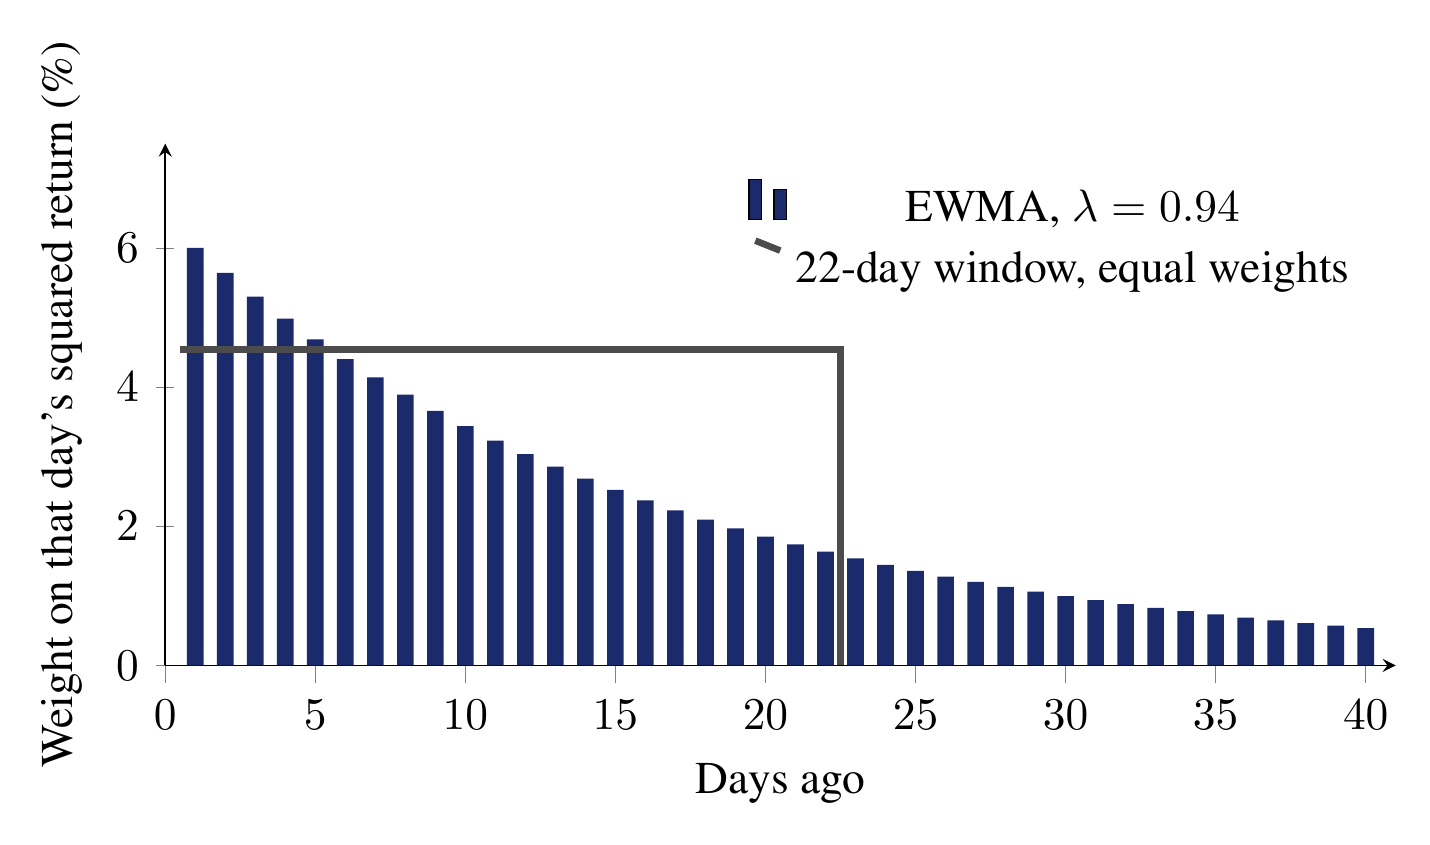
\includegraphics[width=0.85\linewidth]{images/fig11-1-ewma-weights.png}
\caption{Weights on past squared returns. A 22-day historical window gives each day the same weight and then drops it abruptly. EWMA gives the most weight to yesterday and fades older days gradually, so it reacts faster to news and never drops a day all at once.}
\label{fig:11-ewma}
\end{figure}

\textbf{GARCH(1,1)} (generalized autoregressive conditional heteroskedasticity) adds a pull toward a long-run level:
\begin{equation}
  \sigma^2_t = \omega + \alpha\,r^2_{t-1} + \beta\,\sigma^2_{t-1}
  \label{eq:11-garch}
\end{equation}
Here $\alpha$ measures how strongly a new shock moves the forecast, and $\beta$ measures how long the effect lasts. Four quantities follow from the parameters:

\begin{itemize}
  \item \textbf{Persistence} is $\alpha + \beta$, which must be below 1.
  \item The \textbf{long-run variance} is $V = \omega / (1 - \alpha - \beta)$.
  \item Forecasts revert to $V$ geometrically: the expected variance $k$ days ahead is
  \begin{equation}
    E_t[\sigma^2_{t+k}] = V + (\alpha + \beta)^{k-1}\left(\sigma^2_{t+1} - V\right)
    \label{eq:11-forecast}
  \end{equation}
  \item The \textbf{half-life} of a volatility shock, the time for half of it to fade, is $\ln 0.5 / \ln(\alpha + \beta)$.
\end{itemize}

EWMA is the special case $\omega = 0$, $\alpha = 1 - \lambda$, $\beta = \lambda$, with persistence exactly 1, so EWMA forecasts never revert. \textbf{GJR-GARCH} adds a term $\gamma\,r^2_{t-1}\,\mathbf{1}[r_{t-1} < 0]$, where the indicator $\mathbf{1}[\cdot]$ is 1 when its condition holds and 0 otherwise, so falls raise volatility more than rises. This asymmetry is the \textbf{leverage effect}. The parameters are estimated by \textbf{maximum likelihood}: choosing the values that make the observed returns most probable under the model.

\textbf{Realized variance} sums squared returns within a period, such as squared five-minute returns within a day. With enough intraday data it measures that day's variance almost exactly. The \textbf{HAR model} (heterogeneous autoregressive) forecasts tomorrow's realized variance by regressing it on the averages of the last day, week and month.

\textbf{Implied volatility} is the volatility that makes an option's market price equal its model price (Chapter 14). The \textbf{VIX} is the market's 30-day implied volatility for the S\&P 500, computed from a strip of index options. It is a forecast under the \emph{risk-neutral} measure, the probabilities that price assets as if investors did not care about risk, not the real-world probabilities. Investors pay a premium to insure against volatility, so the VIX usually exceeds the volatility that follows. The gap is the \textbf{variance risk premium}.

\textbf{Worked example.} Yesterday's daily volatility estimate was 1.6\% (variance 0.000256), and the market then fell 3\% ($r^2 = 0.0009$).

\begin{itemize}
  \item EWMA with $\lambda = 0.94$: $\sigma^2 = 0.94 \times 0.000256 + 0.06 \times 0.0009 = 0.000295$. Volatility rises to 1.72\% a day, or 27\% annualized.
  \item GARCH with $\omega = 0.000002$, $\alpha = 0.08$ and $\beta = 0.90$:
  \begin{itemize}
    \item $\sigma^2 = 0.000002 + 0.08 \times 0.0009 + 0.90 \times 0.000256 = 0.000304$, or 1.74\% a day.
    \item Persistence is 0.98, so the long-run variance is $0.000002 / 0.02 = 0.0001$: 1\% a day, or 15.9\% a year. The half-life is $\ln 0.5 / \ln 0.98 \approx 34$ trading days (Figure~\ref{fig:11-garch}).
    \item The variance over the next ten days is $10 \times 0.0001 + (0.000304 - 0.0001) \times (1 - 0.98^{10})/(1 - 0.98) = 0.00287$. Ten-day volatility is 5.4\%, or 26.9\% annualized. That is below the 27.7\% you would get by assuming today's 1.74\% persists, because the forecast is already reverting.
  \end{itemize}
\end{itemize}

\begin{figure}[htbp]
\centering
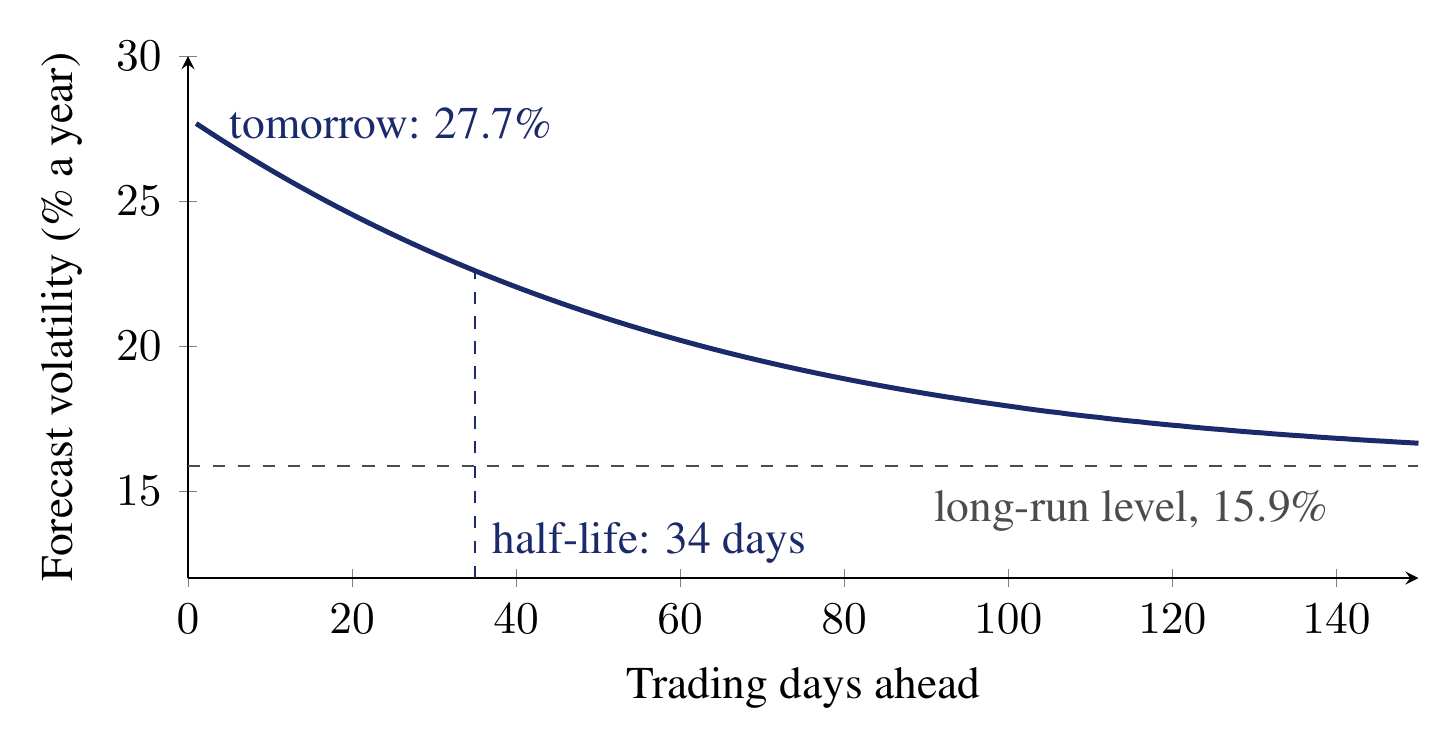
\includegraphics[width=0.85\linewidth]{images/fig11-2-garch-reversion.png}
\caption{A GARCH forecast reverting to its long-run level, from the worked example. After a 3\% fall the forecast for tomorrow is 27.7\% a year; it then decays toward 15.9\%, losing half of the gap every 34 trading days.}
\label{fig:11-garch}
\end{figure}

\textbf{Further reading.} Hull, \emph{Options, Futures, and Other Derivatives} (chapter on estimating volatilities and correlations: EWMA, GARCH, maximum likelihood) and \emph{Risk Management and Financial Institutions}; Tsay, \emph{Analysis of Financial Time Series} (conditional heteroskedastic models); Campbell, Lo and MacKinlay, \emph{The Econometrics of Financial Markets}; Taylor, \emph{Asset Price Dynamics, Volatility, and Prediction}; Poon, \emph{A Practical Guide to Forecasting Financial Market Volatility}.

\section{How it works}
\label{sec:11-how}

Three regularities in daily stock returns, all documented in Chapter 3 (Section~\ref{sec:03-facts}), motivate every model in this chapter.

\begin{itemize}
  \item \textbf{Volatility clustering.} Mandelbrot (1963) observed that large changes tend to be followed by large changes, of either sign, and small changes by small changes. Returns themselves have almost no autocorrelation, but absolute and squared returns are positively autocorrelated, and the autocorrelation decays slowly over weeks and months. A forecastable size combined with an unforecastable sign is exactly what an efficient market with changing risk would produce.
  \item \textbf{Fat tails.} Daily returns have far more extreme days than a normal distribution allows. Part of this is clustering itself: a mixture of calm and turbulent periods, each roughly normal, has fat tails overall. Even after allowing for clustering, the standardized returns $r_t / \sigma_t$ remain somewhat fat-tailed, which is why many applications use Student-$t$ shocks.
  \item \textbf{The leverage effect.} Volatility rises more after falls than after rises of the same size. Black (1976) attributed this to leverage, since a falling share price raises a firm's debt-to-equity ratio and so the riskiness of its equity. The effect is too large to be explained by leverage alone, and it is strongest for the index. Risk premiums and \textbf{volatility feedback}, in which higher expected volatility lowers prices, both contribute.
\end{itemize}

The models differ in how they turn past returns into a forecast.

\begin{itemize}
  \item \textbf{Historical and EWMA} forecasts are smoothing rules with one choice: the window length or $\lambda$.
  \item \textbf{GARCH} models are estimated, have a long-run level and revert toward it. At long horizons their forecasts converge to the \textbf{unconditional variance}, the long-run average, which is right if volatility truly mean-reverts and costly if the long-run level itself shifts.
  \item \textbf{HAR} captures the slow decay of volatility's memory with three regressors, one per horizon. It is linear and estimated by ordinary least squares, which makes it easy to extend.
  \item \textbf{The VIX} is not a model of past returns. It is a market price that can embed information about scheduled events, such as elections and central bank meetings, that no time-series model sees. It also embeds the variance risk premium, so it is biased upward as a forecast.
\end{itemize}

Figure 11.4, from the lab, shows the pattern the models exploit. On U.S. data the bars for returns hover near zero at every lag. The bars for absolute returns are positive at lag 1 and still clearly positive after 50 trading days.

\section{The claim}
\label{sec:11-claim}

\begin{callout}
\textbf{Claim.} Today's volatility forecasts tomorrow's. Forecasts built from past returns, or from option prices, beat a constant forecast by a wide margin, out of sample, at horizons from one day to one month.
\end{callout}

To test the claim we need to be precise on four points.

\begin{itemize}
  \item \textbf{What is forecast.} The target is the variance of the market's return over the next $h$ days, for $h = 1$, 5 and 22. True variance is never observed, so we use a \textbf{proxy}, an observable stand-in: the sum of squared daily returns over those days.
  \item \textbf{Against what.} The weakest benchmark is the \textbf{long-run average}, a constant. Beating it shows that volatility is forecastable at all. The stronger benchmark is a \textbf{random walk} in volatility: last month's variance continues. Beating that shows that a model adds something beyond the obvious.
  \item \textbf{How it is scored.} We use two loss functions, MSE and QLIKE, explained in Section~\ref{sec:11-eval}. The choice matters more than it does for return forecasts.
  \item \textbf{What would count against it.} The claim fails if forecasts beat the long-run average only in sample, or only in calm periods. It weakens if the gain disappears at horizons beyond a few days, or if no model beats the random walk.
\end{itemize}

A second, separate claim concerns use: that an investor who holds less of the market when forecast volatility is high earns a higher Sharpe ratio. Forecastable volatility is necessary for that claim but not sufficient. Expected returns may rise with volatility, and trading has costs.

\section{The original evidence}
\label{sec:11-evidence}

\textbf{ARCH and GARCH.} Engle (1982) introduced the ARCH model, in which today's variance depends on past squared shocks. His first application was to U.K. inflation, not stock returns. Bollerslev (1986) added lagged variance, producing GARCH(1,1), which captures long memory with three parameters. Within a decade GARCH-type models had been fitted to almost every financial series, with the same finding each time: persistence close to 1, so volatility shocks die out over weeks to months. Glosten, Jagannathan and Runkle (1993) added the asymmetric term that bears their initials and found strong leverage effects in U.S. stock returns. Engle shared the 2003 Nobel prize for this work.

\textbf{The low-$R^2$ puzzle and its resolution.} Early out-of-sample tests seemed discouraging. Regressions of daily squared returns on GARCH forecasts gave $R^2$ of only a few percent, and some authors concluded that GARCH forecasts were poor. Andersen and Bollerslev (1998) showed that the problem was the target, not the forecast. A single squared return is an extremely noisy measure of that day's variance, so even a perfect forecast must have a low $R^2$ against it. Measured against realized variance from intraday returns, the same GARCH forecasts explained around half of the variation.

\textbf{Realized volatility and HAR.} Andersen, Bollerslev, Diebold and Labys (2003) treated realized variance as an observable series and modelled it directly. Simple time-series models of realized variance outperformed GARCH models estimated on daily returns. Corsi (2009) proposed the HAR model, motivated by traders who operate at daily, weekly and monthly horizons. It reproduces volatility's long memory with three regressors and has become the standard benchmark for realized-variance forecasts.

\textbf{Horse races.} Hansen and Lunde (2005) compared 330 models on a Deutsche mark--dollar exchange rate and IBM stock returns. For the exchange rate, nothing significantly beat GARCH(1,1). For IBM, GARCH(1,1) was clearly inferior to models with a leverage effect. Poon and Granger (2003) reviewed 93 studies. Implied volatility generally forecast best, followed by historical volatility and GARCH roughly together, and all methods did better than a constant.

\section{Evaluating volatility forecasts}
\label{sec:11-eval}

Scoring a volatility forecast is harder than scoring a return forecast, because the thing being forecast is never observed. Every comparison uses a proxy, such as the sum of squared daily returns. The proxy is unbiased but noisy. The question is whether the noise can change which model wins.

Patton (2011) answered it. With a noisy proxy, only some loss functions are \textbf{robust}: they rank forecasts in the same order as they would against the true variance. Two common ones are robust (Figure~\ref{fig:11-qlike}).

\begin{itemize}
  \item \textbf{MSE}, $(RV - F)^2$, where $RV$ is the proxy and $F$ the forecast. It is robust but dominated by the largest days. A few crisis days can decide the whole comparison.
  \item \textbf{QLIKE}, $\log F + RV/F$, the loss implied by the normal likelihood. It is robust and penalizes forecasts that are too \emph{low} much more than forecasts that are too high, which suits risk management. Because it depends on the ratio $RV/F$, it is not dominated by the level of volatility in crises.
\end{itemize}

\begin{figure}[htbp]
\centering
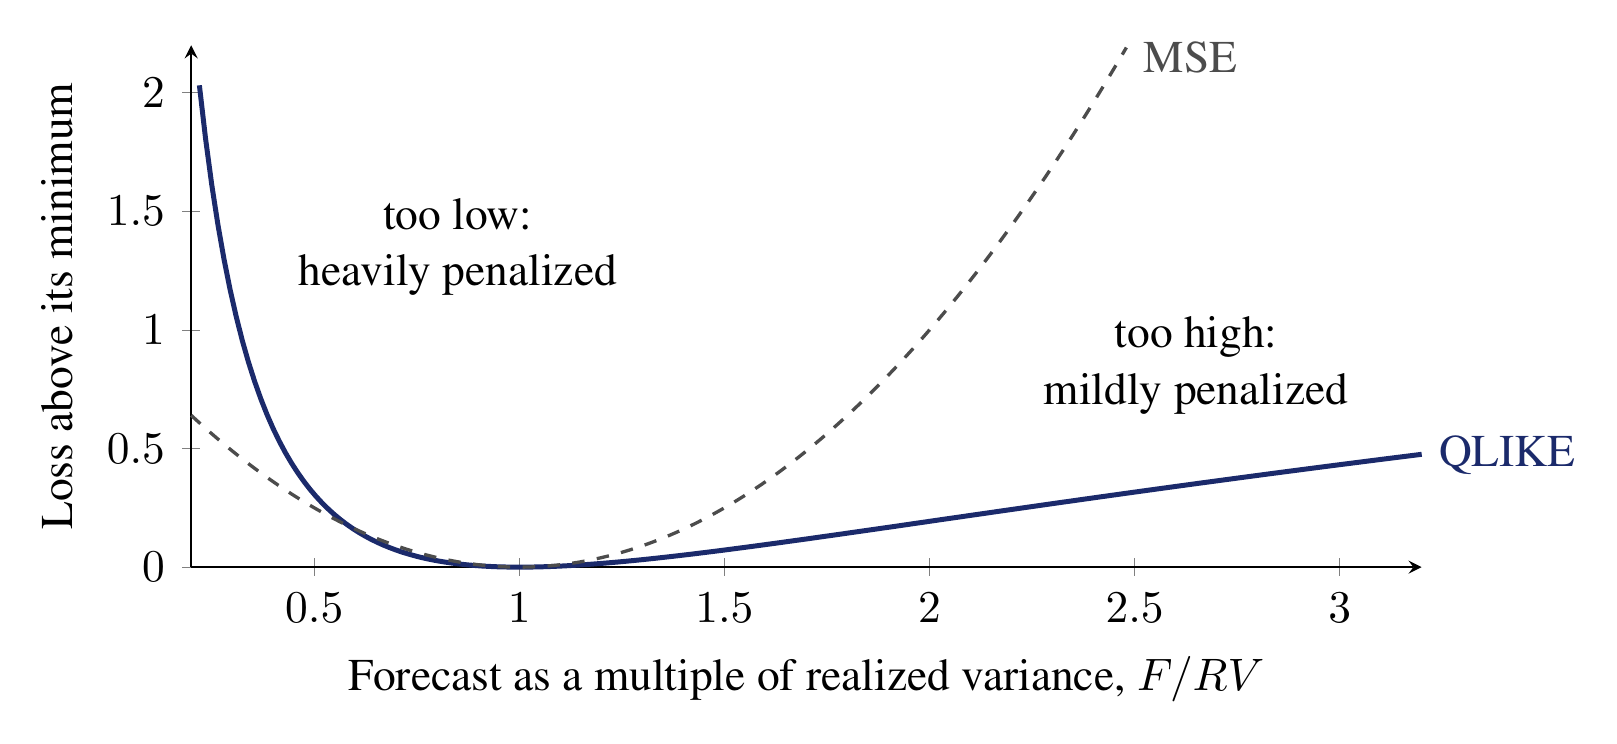
\includegraphics[width=0.85\linewidth]{images/fig11-3-qlike.png}
\caption{Two robust loss functions, measured from their minimum. MSE treats a forecast that is too high and one that is too low symmetrically. QLIKE punishes a forecast that is too low far more than one that is too high: underestimating risk is the costlier mistake.}
\label{fig:11-qlike}
\end{figure}

Others are not robust. Mean absolute error and MSE on volatility rather than variance, both common in early studies, can rank a biased forecast above the true variance when the proxy is noisy. They should be avoided.

Two diagnostics complement the loss comparison.

\begin{itemize}
  \item \textbf{Mincer--Zarnowitz regression.} Regress realized on forecast variance. An unbiased forecast has intercept 0 and slope 1. A slope below 1 means the forecast overreacts, which is typical of the VIX because of the variance risk premium. The $R^2$ measures informativeness but is capped by the noise in the proxy, as Andersen and Bollerslev showed.
  \item \textbf{Diebold--Mariano test} (Chapter 5). Test whether the average loss difference between two models is zero, using Newey--West errors with $h - 1$ lags, since multi-day targets overlap.
\end{itemize}

A fair comparison also requires real-time forecasts. Every parameter must be estimated only on data available at the forecast date, as in the walk-forward design of Chapter 5.

\section{Replication lab: forecasting market volatility}
\label{sec:11-lab}

\begin{callout}
\textbf{Lab 11 at a glance.} \emph{Claim on trial:} volatility is predictable. \emph{Data:} U.S. market returns since 1926, from the daily factors in the Kenneth French library, and, from 1990, the VIX from FRED; both are free. \emph{Code:} runs as a script (\texttt{python lab11.py}) or as a notebook with a prediction prompt before each step.
\end{callout}

\textbf{Part A, stylized facts.} It computes autocorrelations of daily returns and absolute returns at lags 1 to 50, and the correlation between today's return and tomorrow's absolute return (Figure 11.4). Expect the first to hover near zero, the second to stay positive for months, and the third to be negative: the leverage effect.

\textbf{Part B, forecast comparison.} Each trading day from 1990, the lab forecasts the market's variance over the next 1, 5 and 22 days with seven methods:

\begin{center}
\small
\begin{tabularx}{0.9\linewidth}{@{}>{\raggedright\arraybackslash}p{0.20\linewidth}>{\raggedright\arraybackslash}X>{\raggedright\arraybackslash}p{0.33\linewidth}@{}}
\toprule
Method & Forecast & Parameters \\
\midrule
Long-run average & Mean squared return to date & None \\
Random walk & Last 22 days' variance continues & None \\
EWMA & RiskMetrics, $\lambda = 0.94$ & Fixed \\
GARCH(1,1) & Mean-reverting, normal likelihood & Re-estimated yearly on the past 20 years \\
GJR-GARCH & GARCH with the leverage term & Re-estimated yearly \\
HAR & Regression on 1-, 5- and 22-day averages & Re-estimated yearly by OLS \\
VIX & $(\mathrm{VIX}/100)^2 \times h/252$ & None \\
\bottomrule
\end{tabularx}
\end{center}

Each method is scored against the random walk with QLIKE and MSE, with Diebold--Mariano tests and Mincer--Zarnowitz regressions. Figure 11.5 plots one-month forecasts through 2007--2010 against the volatility that followed. Figure 11.6 ranks the methods at each horizon.

\textbf{Part C, crises.} The same losses are computed within 2008--09, 2020 and 2022 (Figure 11.7).

\textbf{Part D, use.} A \textbf{volatility-managed portfolio} holds the market with weight proportional to 1 / last month's realized variance, scaled so its volatility matches the market's, as in Moreira and Muir (2017). The lab reports Sharpe ratio, drawdown and alpha against the market, net of a cost per unit of weight change, with an optional leverage cap (Figure 11.8).

Three design choices affect the results. First, the proxy is built from daily returns, because intraday data are not freely available back to 1926. That makes every model look worse than in studies using five-minute data, but it does not bias the ranking under QLIKE. Second, the HAR model here uses squared daily returns, a much noisier input than the realized variance Corsi used, so expect it to do less well than in the literature. Third, the VIX was redefined in 2003; FRED's VIXCLS uses the current method throughout.

\textbf{What the simulated run shows.} On simulated GJR-GARCH data, the lab recovers what it should. Every dynamic model beats the long-run average by a wide margin. GJR, the true model, ranks first under QLIKE at all three horizons. The simulated VIX shows the upward bias built into it. These results confirm that the code works. They say nothing about real markets. Run the lab on the real data to reach your own verdict.

\section{Stress tests}
\label{sec:11-stress}

\textbf{Horizon.} Forecastability is a short-horizon phenomenon. Because GARCH persistence is below 1, every GARCH forecast converges to the long-run level. Beyond a few months, a constant forecast is hard to beat, and over years, estimates of the long-run level itself drift. At one day to one month, the horizons in the lab, the evidence for forecastability is strong in the literature. The lab lets you measure how fast the advantage over the long-run average shrinks.

\textbf{Crises.} Volatility jumps faster than any model built on past returns can follow. In the first days of October 2008 and of March 2020, every time-series forecast was far too low. QLIKE punishes exactly that error. The models catch up within days, and because they then revert too slowly, they overpredict as the crisis fades. The VIX, as a market price, can react within the day to news and is the obvious candidate to do better at the onset. Figure 11.7 tests whether it did.

\textbf{The 2022 rate shock.} In 2022 stocks fell by about a fifth, but realized volatility stayed moderate, without a single spike. This is a useful contrast with 2008 and 2020. A model that forecasts volatility well can still miss a large, slow decline, because volatility and losses are different things.

\textbf{Estimation window.} GARCH parameters estimated on 20 years that include 2008 differ from those estimated on calmer windows. Persistence near 1 means that small changes in $\alpha + \beta$ produce large changes in long-horizon forecasts. Rerun Part B with \texttt{-{}-window-years 10} and compare.

\textbf{Proxy.} A sum of squared daily returns is noisy, especially at the 1-day horizon, where it is a single squared return. Andersen and Bollerslev (1998) showed that this lowers every model's $R^2$ but, with a robust loss, does not change the ranking. Liu, Patton and Sheppard (2015) compared nearly 400 realized-variance estimators and found that five-minute realized variance is hard to beat. Students with intraday data can replace the proxy and check.

\section{Verdict}
\label{sec:11-verdict}

\begin{callout}
\textbf{Verdict: survives, strongly, at horizons from one day to one month} (as of October 2026). The claim about \emph{using} volatility forecasts to improve a market investor's Sharpe ratio is a separate one, and it \textbf{weakens} once forecasts are made in real time and costs and leverage limits are applied.
\end{callout}

The case for the forecasting claim rests on four findings.

\begin{itemize}
  \item \textbf{It replicates across markets, assets and decades.} Volatility clustering appears in every liquid market studied, back to the nineteenth century. GARCH-type models fitted to them give persistence close to 1.
  \item \textbf{It holds out of sample.} In real-time forecasts, dynamic models beat the long-run average by a wide margin. That is the result Lab 11 is built to check on U.S. data since 1990.
  \item \textbf{It survives the right loss functions.} Early doubts came from evaluating against a noisy proxy with an unsuitable loss. Andersen and Bollerslev (1998) and Patton (2011) removed both problems.
  \item \textbf{It has a plausible mechanism.} News arrives in clusters, and uncertainty is persistent. Nothing about forecastable volatility contradicts market efficiency, since it predicts risk, not returns.
\end{itemize}

The qualifications are about \emph{how much}, not \emph{whether}.

\begin{itemize}
  \item \textbf{Complex models add little over simple ones.} EWMA and GARCH(1,1) are hard to beat for many series. A leverage term helps for equity indices. HAR helps most when realized variance from intraday data is available.
  \item \textbf{The advantage fades with horizon.} Beyond a few months, forecasts converge to a long-run level that is itself uncertain.
  \item \textbf{Every model is late at the onset of a crisis.} Forecasts built from past returns cannot anticipate the first violent day. They are most useful after it.
  \item \textbf{The VIX is informative but biased.} It contains the variance risk premium, so it overstates future volatility on average. It must be adjusted before it is used as a forecast.
\end{itemize}

\section{What investors can use}
\label{sec:11-investors}

\textbf{Risk forecasts, yes.} Any investor sizing positions, setting stop-losses or computing margin should use a volatility forecast that reacts to recent data, such as EWMA or GARCH, rather than a long-run average. This is uncontroversial and is the basis of Value at Risk (Chapter 13).

\textbf{Volatility timing for returns: be skeptical.} Moreira and Muir (2017) found that scaling exposure to the market inversely to last month's variance produced an alpha of about 4.9\% a year over 1926--2015, with similar results for several factors. \textbf{Volatility-targeting} funds and \textbf{risk-parity} strategies, which allocate so that each asset contributes equal risk, apply versions of the idea. Three later findings temper it.

\begin{itemize}
  \item \textbf{Real-time feasibility.} Cederburg, O'Doherty, Wang and Yan (2020) tested 103 equity strategies. The alphas in \textbf{spanning regressions}, regressions of the managed portfolio on the original, were real, but exploiting them required combining the managed and unmanaged portfolios with weights estimated in sample. Implemented out of sample, the managed versions generally did no better than the originals, because the spanning regressions were unstable.
  \item \textbf{Leverage.} The managed portfolio's weight on the market often exceeds 1 in calm periods. In the lab's simulated run it averaged 1.4 and peaked near 10. Capping leverage at a realistic level reduces the gains.
  \item \textbf{Costs and crowding.} Turnover is high when volatility changes quickly, and volatility-targeting funds all sell at the same time, which can deepen the declines they are trying to avoid.
\end{itemize}

The benefit is clearer for momentum, where crashes follow high volatility (Barroso and Santa-Clara 2015; Chapter 9), than for the market.

\textbf{Questions to ask a manager who uses volatility targeting:}

\begin{itemize}
  \item What volatility forecast do you use, and how quickly does it react?
  \item What is the maximum leverage, and what happens to turnover in a volatility spike?
  \item Is the backtest scaled using information available at the time, or using full-sample volatility?
  \item How did the strategy perform in February 2018 and March 2020, when volatility jumped within days?
\end{itemize}

\begin{callout}
\textbf{What Failed: selling volatility before February 5, 2018.} For years before 2018, products that bet against volatility were among the best performers in the market. The VelocityShares Daily Inverse VIX Short-Term ETN (XIV) earned the variance risk premium by shorting VIX futures, and it held \$1.9 billion in assets. On February 5, 2018, the VIX rose 115.6\%, its largest one-day increase ever. XIV lost 96.3\% of its value that day, and Credit Suisse, its issuer, closed it within weeks.

The episode does not contradict this chapter. Volatility forecasts are informative on average. But a forecast that volatility will stay low is weakest exactly when it matters most: at the onset of a spike. A strategy that earns a small premium most days and loses almost everything on one day can look excellent in any backtest that misses that day. Chapter 13 returns to this problem.
\end{callout}

\section{Open questions}
\label{sec:11-open}

\begin{itemize}
  \item \textbf{Does volatility timing pay after costs?} The evidence for the market is mixed. Does it hold for factors such as momentum, and in other countries?
  \item \textbf{What is the right long-run level?} GARCH forecasts revert to a constant, but the evidence suggests slow-moving changes in average volatility, linked to the business cycle and macroeconomic uncertainty. Component GARCH and GARCH-MIDAS models try to capture this. Do they forecast better at long horizons?
  \item \textbf{Can machine learning beat HAR?} Recent studies add many predictors, such as news, macroeconomic data and other assets' volatilities. Do the gains survive the out-of-sample discipline of Chapters 4 and 5?
  \item \textbf{What does the VIX know?} Implied volatility combines a forecast with a risk premium. Can the two be separated well enough to improve the forecast?
\end{itemize}

\section*{Exercises}
\addcontentsline{toc}{section}{Exercises}

\subsection*{Conceptual (all readers)}

\begin{enumerate}
  \item A GARCH(1,1) model has $\omega = 0.000003$, $\alpha = 0.10$ and $\beta = 0.88$. (a) What are the long-run daily and annualized volatilities? (b) What is the half-life of a shock? (c) If tomorrow's variance forecast is 0.0004, what is the forecast volatility over the next 22 days, annualized?
  \item Show that EWMA is GARCH(1,1) with $\omega = 0$. What does this imply for EWMA forecasts at long horizons?
  \item A colleague argues that because volatility is forecastable, markets cannot be efficient. Explain why forecastable volatility is consistent with efficiency, and what evidence would change your answer.
\end{enumerate}

\subsection*{Lab extensions (technical readers)}

\begin{enumerate}
  \setcounter{enumi}{3}
  \item Part A: compute the autocorrelations of squared returns as well as absolute returns. Which decays faster, and why might extreme days explain the difference?
  \item Part B: rank the models by MSE instead of QLIKE. Does the ranking change? Which days drive the MSE comparison?
  \item Part B: estimate GARCH with Student-$t$ shocks, using the option \texttt{dist="t"} of \texttt{fit\_garch}. Does it forecast better than the normal version?
  \item Part B: regress realized variance on both the GJR forecast and the VIX. Does each add information? Compare the VIX's Mincer--Zarnowitz slope with 1 and explain.
  \item Part C: for the first ten trading days of October 2008 and of March 2020, plot each forecast against realized variance. How many days did each model take to catch up?
  \item Part D: rescale the managed portfolio using only past data and cap the weight at 1.5. How much of the alpha survives? Compare with Cederburg et al.\ (2020).
\end{enumerate}

\section*{References}
\addcontentsline{toc}{section}{References}

\begin{itemize}
  \item Andersen, T. G. and Bollerslev, T. (1998). Answering the Skeptics: Yes, Standard Volatility Models Do Provide Accurate Forecasts. \emph{International Economic Review} 39(4): 885--905.
  \item Andersen, T. G., Bollerslev, T., Diebold, F. X. and Labys, P. (2003). Modeling and Forecasting Realized Volatility. \emph{Econometrica} 71(2): 579--625.
  \item Barroso, P. and Santa-Clara, P. (2015). Momentum Has Its Moments. \emph{Journal of Financial Economics} 116(1): 111--120.
  \item Black, F. (1976). Studies of Stock Price Volatility Changes. \emph{Proceedings of the 1976 Meetings of the American Statistical Association, Business and Economic Statistics Section}: 177--181.
  \item Bollerslev, T. (1986). Generalized Autoregressive Conditional Heteroskedasticity. \emph{Journal of Econometrics} 31(3): 307--327.
  \item Cederburg, S., O'Doherty, M. S., Wang, F. and Yan, X. (2020). On the Performance of Volatility-Managed Portfolios. \emph{Journal of Financial Economics} 138(1): 95--117.
  \item Corsi, F. (2009). A Simple Approximate Long-Memory Model of Realized Volatility. \emph{Journal of Financial Econometrics} 7(2): 174--196.
  \item Engle, R. F. (1982). Autoregressive Conditional Heteroscedasticity with Estimates of the Variance of United Kingdom Inflation. \emph{Econometrica} 50(4): 987--1007.
  \item Glosten, L. R., Jagannathan, R. and Runkle, D. E. (1993). On the Relation between the Expected Value and the Volatility of the Nominal Excess Return on Stocks. \emph{Journal of Finance} 48(5): 1779--1801.
  \item Hansen, P. R. and Lunde, A. (2005). A Forecast Comparison of Volatility Models: Does Anything Beat a GARCH(1,1)? \emph{Journal of Applied Econometrics} 20(7): 873--889.
  \item J.P. Morgan/Reuters (1996). \emph{RiskMetrics---Technical Document} (4th ed.). New York: Morgan Guaranty Trust Company.
  \item Liu, L. Y., Patton, A. J. and Sheppard, K. (2015). Does Anything Beat 5-Minute RV? A Comparison of Realized Measures across Multiple Asset Classes. \emph{Journal of Econometrics} 187(1): 293--311.
  \item Mandelbrot, B. (1963). The Variation of Certain Speculative Prices. \emph{Journal of Business} 36(4): 394--419.
  \item Moreira, A. and Muir, T. (2017). Volatility-Managed Portfolios. \emph{Journal of Finance} 72(4): 1611--1644.
  \item Patton, A. J. (2011). Volatility Forecast Comparison Using Imperfect Volatility Proxies. \emph{Journal of Econometrics} 160(1): 246--256.
  \item Poon, S.-H. and Granger, C. W. J. (2003). Forecasting Volatility in Financial Markets: A Review. \emph{Journal of Economic Literature} 41(2): 478--539.
\end{itemize}

\textbf{Data:} Kenneth R. French Data Library, Fama/French 3 Factors [Daily]. Chicago Board Options Exchange, CBOE Volatility Index: VIX [VIXCLS], retrieved from FRED, Federal Reserve Bank of St.\ Louis.

% Chapter 12 -- The Low-Risk Anomaly
% Requires: amsmath, amssymb, booktabs, array, tabularx, graphicx, tcolorbox (breakable, skins), hyperref or url.
% Defines the callout box only if the preamble has not.
\providecolor{fenavy}{HTML}{1B2A6B}
\providecolor{feshade}{HTML}{F3F5FA}
\makeatletter
\@ifundefined{callout}{%
  \newtcolorbox{callout}{breakable, enhanced,
    colback=white, colframe=gray!70, boxrule=0.5pt, arc=1mm,
    borderline west={2.5pt}{0pt}{gray!70},
    left=8pt, right=8pt, top=4pt, bottom=4pt}%
}{}
\makeatother

\chapter{The Low-Risk Anomaly}
\label{ch:12}

The capital asset pricing model makes one central prediction: assets that move more with the market should earn more. Double the beta, double the expected excess return. It is the first model most finance students learn and the one most practitioners still use to set hurdle rates.

The prediction was also among the first to be tested, and it failed early. In the 1970s Black, Jensen and Scholes found that the relation between beta and average return was positive but far flatter than the CAPM implied. Since then the finding has been extended in two directions. Stocks with low \emph{volatility}, not just low beta, have earned more than their risk suggests. And the pattern appears in other countries and asset classes. It is now usually called the \textbf{low-risk anomaly}.

This chapter asks whether the low-risk anomaly is a real and usable premium or something weaker: a tilt toward small or profitable firms, a disguised bet on interest rates, or a pattern that faded once low-volatility funds became popular after 2010.

By the end of the chapter you will be able to:

\begin{itemize}
  \item estimate a beta, split total risk into systematic and idiosyncratic parts, and compute a CAPM alpha;
  \item draw the security market line and explain how leverage constraints flatten it;
  \item build a beta-neutral betting-against-beta portfolio and explain why a naive low-minus-high portfolio can lose money despite a positive alpha;
  \item state the weak and strong forms of the low-risk claim and summarize the evidence for each;
  \item compare the explanations: leverage constraints, lottery preferences, benchmarking, and missing risk factors;
  \item judge whether a minimum-volatility or BAB fund delivers what its backtest promises.
\end{itemize}

\section{Foundations: beta, the CAPM and the security market line}
\label{sec:12-foundations}

\textbf{Beta} measures how much an asset moves with the market:
\begin{equation}
  \beta_i = \frac{\mathrm{Cov}(R_i, R_m)}{\mathrm{Var}(R_m)}
  \label{eq:12-beta}
\end{equation}
In practice it is the slope of a regression of the asset's excess return on the market's excess return. The market itself has a beta of 1. A stock with a beta of 1.5 tends to rise 1.5\% when the market rises 1\%, and to fall 1.5\% when it falls 1\%.

\textbf{Total risk} splits into two parts. \textbf{Systematic risk} is $\beta_i^2\,\mathrm{Var}(R_m)$. \textbf{Idiosyncratic risk} is the variance of the regression residual, which diversification removes. Two stocks can have the same volatility but very different betas.

The \textbf{CAPM} (Sharpe 1964, Lintner 1965) says that only systematic risk is priced:
\begin{equation}
  E[R_i] - R_f = \beta_i \left(E[R_m] - R_f\right)
  \label{eq:12-capm}
\end{equation}
Plotting expected return against beta gives the \textbf{security market line (SML)}. It is a straight line through the risk-free rate at $\beta = 0$ and the market at $\beta = 1$, so its slope equals the market premium. Idiosyncratic risk earns nothing, because investors can diversify it away for free.

\textbf{Alpha} (Jensen's alpha) is the intercept $\alpha_i$ in the regression
\begin{equation}
  R_i - R_f = \alpha_i + \beta_i (R_m - R_f) + \varepsilon_i
  \label{eq:12-alpha}
\end{equation}
It measures average return beyond what beta explains. Under the CAPM every alpha is zero. A \textbf{multifactor alpha} adds other factors to the regression, such as size, value and momentum (Chapter 8).

The CAPM assumes that investors can borrow and lend freely at the risk-free rate. An investor who wants more risk than the market then borrows and buys the market, or any efficient portfolio. Many investors cannot do this. Mutual funds and pension plans face limits on \textbf{leverage}, borrowing to hold more than their capital. Individuals face \textbf{margin} requirements and pay more than the risk-free rate to borrow. Black (1972) showed that without riskless borrowing the SML is still straight but flatter: it starts at the return on a \textbf{zero-beta portfolio}, a portfolio uncorrelated with the market, which lies above the risk-free rate.

\textbf{Worked example.} The risk-free rate is 3\% and the market premium is 6\% (Figure~\ref{fig:12-sml}).

\begin{itemize}
  \item Stock A has a beta of 0.6 and has averaged 9\%. The CAPM predicts $3\% + 0.6 \times 6\% = 6.6\%$, so A's alpha is $+2.4\%$.
  \item Stock B has a beta of 1.5 and has averaged 10\%. The CAPM predicts $3\% + 1.5 \times 6\% = 12\%$, so B's alpha is $-2\%$.
  \item An investor who can borrow at 3\% can lever A to a beta of 1. She holds $1/0.6 = 1.67$ dollars of A for each dollar of capital and borrows the remaining 0.67 dollars. Her expected return is $3\% + 1.67 \times (9\% - 3\%) = 13\%$, compared with 9\% for the market at the same beta. Even at a borrowing rate of 5\%, she earns $1.67 \times 9\% - 0.67 \times 5\% \approx 11.7\%$.
  \item An investor who cannot borrow and wants a beta above 1 must buy B instead. If many investors are in that position, they bid up high-beta stocks such as B and push down their future returns. That is the core of the leverage-constraint explanation in Section~\ref{sec:12-explanations}.
\end{itemize}

\begin{figure}[htbp]
\centering
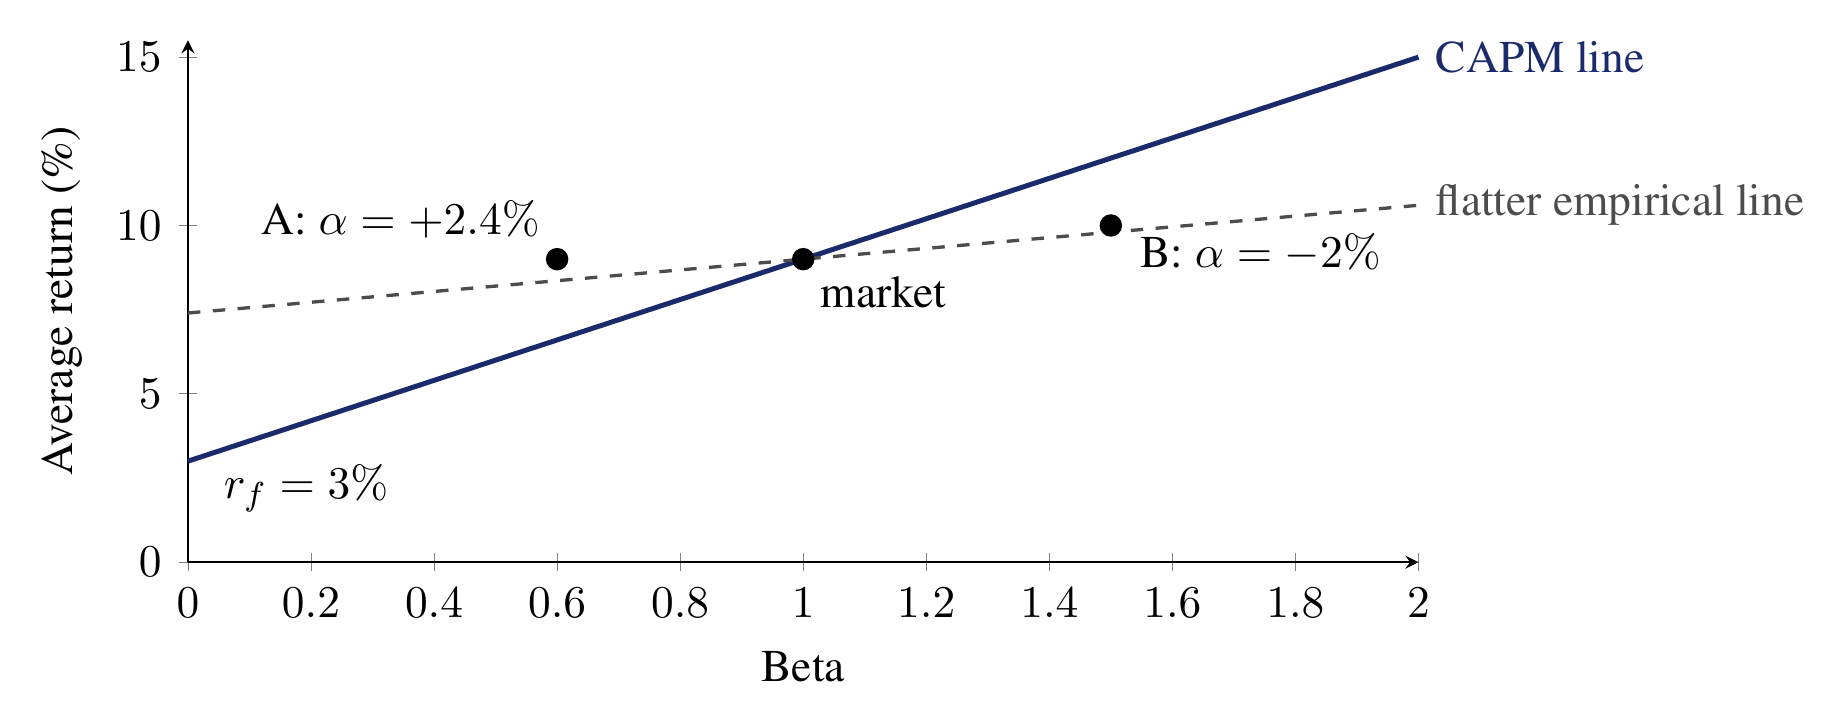
\includegraphics[width=0.85\linewidth]{images/fig12-1-sml.png}
\caption{The security market line in the worked example. The CAPM line runs from the risk-free rate of 3\% through the market at a beta of 1. Stock A lies above it (positive alpha) and stock B below it (negative alpha), so the line through A and B is flatter than the CAPM predicts.}
\label{fig:12-sml}
\end{figure}

\textbf{Further reading.} Bodie, Kane and Marcus, \emph{Investments} (the CAPM, the index model and beta estimation, and empirical tests of the CAPM); Cochrane, \emph{Asset Pricing} (beta pricing models and their tests); Campbell, Lo and MacKinlay, \emph{The Econometrics of Financial Markets} (tests of the CAPM); Ang, \emph{Asset Management} (low-risk anomalies from an investor's viewpoint).

\section{How it works}
\label{sec:12-how}

There are three ways to sort stocks on risk, and the literature uses all three.

\begin{itemize}
  \item \textbf{Beta.} Estimate each stock's beta from past returns, typically 36 to 60 months of monthly data or a year of daily data. Sort into portfolios. This tests the CAPM directly.
  \item \textbf{Total volatility.} Sort on the standard deviation of past daily returns, often over one to three months. This needs no market model, and it is how most low-volatility funds work.
  \item \textbf{Idiosyncratic volatility.} Sort on the volatility of residuals from a factor model, usually the Fama--French three-factor model. Under the CAPM this risk should not be priced at all, so a negative relation is especially puzzling.
\end{itemize}

The three measures are strongly correlated. High-beta stocks tend to be volatile, and volatile stocks tend to have high idiosyncratic risk. Separating them is one of the open problems in this chapter.

A flat SML shows up in two ways. The first is \emph{alphas}: low-risk portfolios have positive CAPM alphas and high-risk portfolios negative ones. The second is a \emph{long-short portfolio}. The naive version, long low-risk stocks and short high-risk stocks, has a strongly negative beta. It loses money in rising markets even if the SML is flat, and its average return can be negative while its alpha is positive. \textbf{Betting against beta (BAB)} fixes this. It levers the low-beta leg up to a beta of 1 and scales the high-beta leg down to a beta of 1, so the portfolio is \textbf{beta-neutral}, with no net exposure to the market (Figure~\ref{fig:12-bab}):
\begin{equation}
  r_{\mathrm{BAB}} = \frac{r_L - r_f}{\beta_L} - \frac{r_H - r_f}{\beta_H}
  \label{eq:12-bab}
\end{equation}
If the SML is flat, this portfolio earns a positive return with no market exposure. The betas must be \textbf{ex ante}, estimated from data available when the portfolio is formed. Otherwise the construction looks ahead (Section~\ref{sec:02-lookahead}).

\begin{figure}[htbp]
\centering
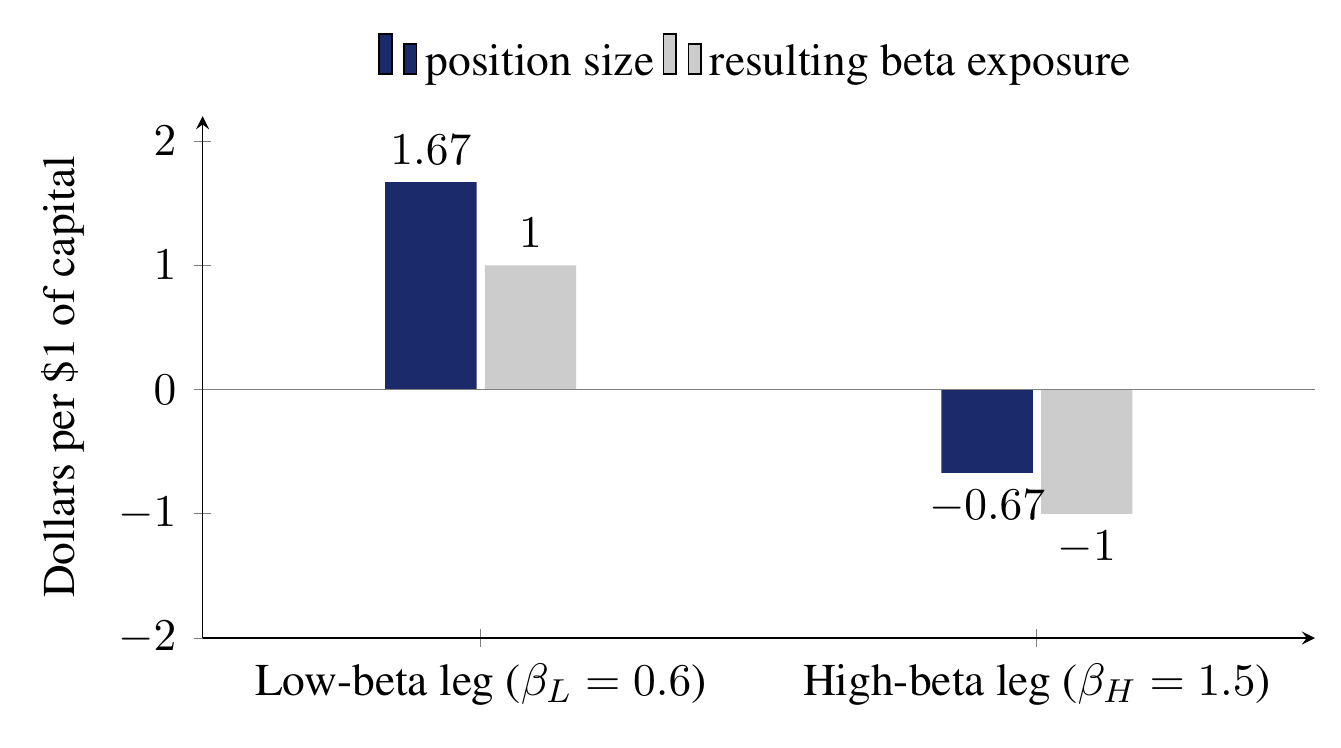
\includegraphics[width=0.85\linewidth]{images/fig12-2-bab.png}
\caption{Building a BAB portfolio from the worked example. Per dollar of capital, it holds \$1.67 of the low-beta stock ($\beta_L = 0.6$) and shorts \$0.67 of the high-beta stock ($\beta_H = 1.5$). Each leg then carries a beta exposure of 1, in opposite directions, so the portfolio's beta is zero.}
\label{fig:12-bab}
\end{figure}

The explanations divide into those that treat the anomaly as \textbf{mispricing} and those that treat it as \textbf{compensation for a risk the CAPM misses}. Section~\ref{sec:12-explanations} sets them out. They matter because they predict different things about when the anomaly should be strongest, and about whether it should survive its own popularity.

\section{The claim}
\label{sec:12-claim}

\begin{callout}
\textbf{Claim.} Low-beta and low-volatility stocks earn higher risk-adjusted returns than the CAPM predicts. The security market line is flatter than the market premium, and a beta-neutral portfolio that is long low-risk stocks and short high-risk stocks earns a positive alpha.
\end{callout}

To test it we need to specify four things.

\begin{itemize}
  \item \textbf{The strong form.} The SML is not just flat but \emph{inverted}: low-risk stocks earn higher raw returns, not just higher risk-adjusted returns. Some studies of volatility sorts find this. Most studies of beta sorts find a flat or weakly positive relation instead.
  \item \textbf{The weak form.} The SML is positive but flatter than the CAPM predicts, so low-beta stocks have positive alphas. This is what Black, Jensen and Scholes found, and it is the claim tested here.
  \item \textbf{Risk adjustment.} A CAPM alpha is the natural first test. The claim is more interesting if the alpha survives the size, value and momentum factors, and more interesting still if it survives profitability and interest-rate exposure.
  \item \textbf{What would count against it.} The claim weakens if the alpha is concentrated in micro-caps, if it disappears after controlling for other known factors, or if it has faded since the strategy became popular. It fails if a beta-neutral, tradable version earns nothing after costs.
\end{itemize}

\section{The original evidence}
\label{sec:12-evidence}

\textbf{A flat line from the start.} Black, Jensen and Scholes (1972) sorted NYSE stocks from 1931 to 1965 into ten portfolios by past beta, so that estimation error in individual betas would average out. Average returns rose with beta, but much less than the CAPM predicted. Low-beta portfolios had positive alphas and high-beta portfolios negative ones. Fama and MacBeth (1973) confirmed a positive but modest slope. Haugen and Heins (1975) reported that low-volatility portfolios had matched or beaten high-volatility ones, and Fama and French (1992) found almost no relation between beta and average return from 1963 to 1990 once size was controlled for.

\textbf{Idiosyncratic volatility.} Ang, Hodrick, Xing and Zhang (2006) sorted U.S. stocks on idiosyncratic volatility measured over the previous month. The highest-volatility quintile earned 1.06\% a month less than the lowest, and its Fama--French alpha was 1.31\% a month lower. The result was a strong form of the anomaly: an inverted relation between this risk and raw returns. Their 2009 paper found the same pattern in 23 developed markets.

\textbf{From anomaly to strategy.} Baker, Bradley and Wurgler (2011) documented the low-risk anomaly for investors and argued that benchmarking prevents institutions from exploiting it. Frazzini and Pedersen (2014) built the BAB factor described in Section~\ref{sec:12-how} from individual stocks, using rank weights and shrunk betas. In U.S. stocks from 1926 to 2012 it had a Sharpe ratio of 0.78. It earned significant alphas after size, value, momentum and liquidity controls, in 19 international equity markets, and in Treasury bonds, corporate bonds and futures. They also found that BAB returns were lower when funding constraints were tight, which their leverage-constraint theory predicts.

By 2014 the low-risk anomaly looked like one of the best-documented patterns in finance. Low-volatility index funds launched in the United States around 2011 and grew quickly.

\section{Explanations}
\label{sec:12-explanations}

\textbf{Leverage constraints.} Black (1972) and Frazzini and Pedersen (2014) argue that investors who want high expected returns but cannot borrow overweight high-beta stocks instead of levering the market. That bids up high-beta stocks and flattens the SML. The theory predicts that constrained investors, such as mutual funds and individuals, hold high-beta portfolios, and that BAB does worse when funding tightens. Both predictions have empirical support.

\textbf{Lottery preferences.} Some investors like stocks with a small chance of a very large gain, as with a lottery ticket, and overpay for them. Barberis and Huang (2008) derive this from probability weighting in prospect theory. Bali, Cakici and Whitelaw (2011) found that stocks with the largest daily returns over the past month subsequently underperform, and that this absorbs much of the idiosyncratic volatility effect. Lottery demand explains volatility sorts more naturally than beta sorts.

\textbf{Benchmarking.} Most institutional managers are judged against a capitalization-weighted index. For them, a low-beta stock with positive alpha is not attractive: it adds \textbf{tracking error}, the volatility of the return difference from the benchmark, and lags in rising markets. Baker, Bradley and Wurgler (2011) argue that this keeps institutions from correcting the mispricing. Part D of the lab measures how large that tracking error is.

\textbf{Overpricing that is hard to short.} Liu, Stambaugh and Yuan (2018) found that the beta anomaly comes from beta's correlation with idiosyncratic volatility, and that it is concentrated among overpriced stocks, where short-selling is costly.

\textbf{Missing risk factors.} Other explanations treat the alpha as compensation for risks the CAPM omits.

\begin{itemize}
  \item \emph{Profitability and investment.} Low-risk stocks tend to be large, profitable and conservative in investment. Fama and French (2016) found that their five-factor model, which adds profitability and investment factors, explains much of the low-beta and low-volatility alphas.
  \item \emph{Interest rates.} Low-volatility stocks, such as utilities and consumer staples, behave partly like bonds. Driessen, Kuiper, Nazliben and Beilo (2019) found that low-volatility portfolios lose value when rates rise and that an interest-rate premium explains part, but not all, of the anomaly. Over 1981--2020 bond yields fell almost continuously, which would have flattered any bond-like equity strategy.
  \item \emph{Conditional betas.} Cederburg and O'Doherty (2016) found that betas vary over time in ways that bias unconditional alphas, and that modelling time-varying betas largely eliminates the alpha gap between low- and high-beta stocks.
\end{itemize}

The explanations are not mutually exclusive. Asness, Frazzini, Gormsen and Pedersen (2020) split BAB into a bet against correlation, which they link to leverage constraints, and a bet against volatility, which they link to lottery demand, and report that both earn returns.

\section{Replication lab: the security market line since 1963}
\label{sec:12-lab}

\begin{callout}
\textbf{Lab 12 at a glance.} \emph{Claim on trial:} low-risk stocks earn more than the CAPM predicts. \emph{Data:} ten portfolios formed on market beta, on total variance and on residual variance, each value- and equal-weighted, from July 1963, from the Kenneth French library; the Fama--French and momentum factors; the 10-year Treasury yield from FRED; optionally, AQR's published BAB factor for comparison. All are free. \emph{Code:} runs as a script (\texttt{python lab12.py}) or as a notebook with a prediction prompt before each step.
\end{callout}

\textbf{Part A, the SML.} For each set of decile portfolios, the lab estimates average excess return, realized beta, CAPM alpha and four-factor alpha, and the slope of average return on beta across the deciles. Figure 12.3 plots the deciles against the CAPM line, which runs from the origin through the market.

\textbf{Part B, long-short portfolios.} Two constructions for each sort:

\begin{center}
\small
\begin{tabularx}{0.9\linewidth}{@{}>{\raggedright\arraybackslash}p{0.19\linewidth}>{\raggedright\arraybackslash}X>{\raggedright\arraybackslash}X>{\raggedright\arraybackslash}p{0.17\linewidth}@{}}
\toprule
Construction & Long & Short & Beta \\
\midrule
Low minus high & Three lowest-risk deciles & Three highest-risk deciles & Strongly negative \\
BAB-style & Low leg $\times\, 1/\beta_L$ & High leg $\times\, 1/\beta_H$ & About zero \\
\bottomrule
\end{tabularx}
\end{center}

The betas are estimated from the previous 60 months of each leg's returns, so the portfolio uses only information available at the time. Figure 12.4 plots cumulative returns.

This is a simpler construction than Frazzini and Pedersen's. They use individual stocks with rank weights. The lab uses published portfolios, which anyone can reproduce in minutes. Expect it to show the same pattern with smaller numbers, partly because it does not tilt toward small stocks. Comparing it with AQR's factor (optional) shows how much the construction matters.

\textbf{Part C, stress tests.} Equal versus value weights, three subperiods (1963--1990, 1991--2009, 2010 onward), interest-rate exposure, calendar-year returns in 2008, 2020 and 2022, and rolling ten-year alphas (Figures 12.5 and 12.6).

\textbf{Part D, the investor's view.} The lowest-volatility and lowest-beta quintiles against the market: Sharpe ratio, alpha, drawdown, tracking error and the share of years in which they trailed the market (Figure 12.7).

\textbf{What the simulated run shows.} On simulated data built with a flat SML, the lab recovers what it should. The slope across beta deciles is far below the market premium. The BAB-style portfolios have betas near zero and positive alphas. The low-minus-high portfolio sorted on beta loses money on average despite its positive alpha, which illustrates why the construction matters. These results confirm that the code works. They say nothing about real markets. Run the lab on the real data to reach your own verdict.

\section{Stress tests}
\label{sec:12-stress}

\textbf{Micro-caps and weighting.} Novy-Marx and Velikov (2022) found that AQR's BAB factor, through its rank weighting and leverage, commits on average about \$1.05 of each dollar to the smallest 1\% of stocks by market capitalization. Those stocks are expensive to trade (Chapter 6). After costs BAB still earned positive returns, but they attribute part of them to exposure to profitability and investment. The lab's equal- versus value-weighted comparison is a coarse version of this test. If the effect is much stronger in equal-weighted portfolios, small stocks are doing much of the work (Section~\ref{sec:02-microcaps}).

\textbf{Other factors.} Fama and French (2016) found that profitability and investment factors absorb much of the low-risk alphas. The lab uses four factors, so its alphas probably overstate what remains. Exercise 6 adds the five-factor model.

\textbf{Interest rates.} If low-risk stocks are partly bonds, their alpha includes a bond premium earned during four decades of falling yields. The lab regresses the long-short returns and the low-risk leg on the market and on monthly changes in the 10-year yield. A negative coefficient means the strategy loses when yields rise. 2022 is the natural out-of-sample test: yields rose sharply, and stocks and bonds fell together.

\textbf{Crowding.} Low-volatility funds grew rapidly after 2011. If the anomaly reflected mispricing, the inflows should have raised the prices of low-risk stocks, boosting returns at first and lowering them afterward. The lab's 2010-onward subperiod and the rolling alphas in Figure 12.5 show whether the premium has shrunk.

\textbf{Drawdowns.} Low-risk portfolios are meant to protect in crashes. Check 2008 and March 2020. A beta-neutral BAB portfolio is a different matter. It is long levered low-beta stocks and short high-beta stocks, and it can lose heavily when high-beta stocks rebound sharply, as in 2009 and in the 2020 recovery.

\textbf{Estimation error in beta.} Sorting on noisy past betas means the low-beta portfolio contains stocks whose true betas are higher than estimated, and the reverse. This biases the SML toward flatness even if the CAPM holds. Black, Jensen and Scholes used portfolios to reduce the problem, and the French portfolios do the same. Novy-Marx and Velikov (2022) also showed that Frazzini and Pedersen's beta estimator, which combines correlations and volatilities measured over different windows, introduces its own biases.

\section{Verdict}
\label{sec:12-verdict}

\begin{callout}
\textbf{Verdict: weakens} (as of October 2026). The weak form of the claim, that the security market line is flatter than the CAPM predicts, is one of the most robust findings in empirical finance. The strong form, that low-risk stocks earn a distinct premium that a beta-neutral portfolio can harvest, is weaker. Its size depends heavily on construction and on micro-caps, much of it overlaps with profitability, investment and interest-rate exposure, and the evidence that it is a separate premium is weaker than it looked in 2014.
\end{callout}

What survives:

\begin{itemize}
  \item \textbf{The flat SML.} Since Black, Jensen and Scholes, beta sorts have shown a relation between beta and average return that is much flatter than the market premium, in the United States and abroad. A CAPM hurdle rate overstates the expected return of high-beta assets relative to low-beta ones.
  \item \textbf{Low risk without lower returns.} Low-volatility portfolios have delivered returns close to the market's with substantially less volatility, so their Sharpe ratios have been higher. For an unconstrained investor that is useful.
\end{itemize}

What weakens it:

\begin{itemize}
  \item \textbf{Construction.} Rank-weighted, stock-level BAB factors put much of their capital in the smallest stocks (Novy-Marx and Velikov 2022). Portfolio-based versions, like the lab's, earn less.
  \item \textbf{Overlap with other factors.} Profitability and investment factors explain much of the alpha (Fama and French 2016). Time-varying betas explain much of the rest (Cederburg and O'Doherty 2016).
  \item \textbf{Interest rates.} Low-risk stocks behave partly like bonds, and the sample is dominated by four decades of falling yields.
  \item \textbf{Crowding.} Inflows into low-volatility funds after 2011 are likely to have raised the prices of low-risk stocks, which would make past returns a poor guide to future ones.
\end{itemize}

The verdict would move to \emph{survives} if a beta-neutral, value-weighted version continued to earn a significant alpha against the five-factor model and interest-rate exposure out of sample. It would move to \emph{fails} if the post-2010 alphas proved to be inflow effects that reversed.

\section{What investors can use}
\label{sec:12-investors}

\textbf{Minimum-volatility funds} are the most common way investors access the low-risk anomaly. They hold a portfolio of stocks chosen or optimized for low volatility, usually long-only and without leverage. Three things are worth knowing before buying one.

\begin{itemize}
  \item \textbf{They are low-beta, not market-neutral.} With a beta around 0.7 to 0.8, a minimum-volatility fund will usually trail the market in strong bull markets and beat it in crashes. The case for holding one rests on a better ratio of return to risk, not higher returns.
  \item \textbf{Tracking error is large.} For an investor measured against the market, the fund can lag for years at a time. Part D of the lab shows how often. Investors who cannot tolerate that, including most institutions, are the reason Baker, Bradley and Wurgler think the anomaly persists. Investors who abandon the strategy after a few bad years lose most of its benefit.
  \item \textbf{Hidden exposures.} These funds tend to overweight utilities, consumer staples and real estate, which are sensitive to interest rates. Their valuations can rise with the strategy's popularity. An investor should check the sector weights, the valuation relative to the market, and how the fund behaved when yields rose.
\end{itemize}

\textbf{BAB-style funds}, long levered low-beta stocks and short high-beta stocks, are a different product. They are market-neutral, carry the micro-cap and leverage issues discussed above, and can suffer sharp losses when high-beta stocks rebound.

\textbf{Questions to ask a manager offering a low-volatility or defensive equity strategy:}

\begin{itemize}
  \item Is the portfolio sorted on beta, on volatility or on an optimizer's estimate of risk? How much tracking error should I expect against the market?
  \item What are the strategy's sector weights and interest-rate sensitivity? How did it perform in 2022?
  \item Does the backtest include micro-caps? What is its alpha against the five-factor model?
  \item How have valuations of low-volatility stocks changed since the strategy became popular?
\end{itemize}

\begin{callout}
\textbf{What Failed: the CAPM as a hurdle rate.} The CAPM's empirical problems have been known since the early 1970s, yet it remains the standard way to set the cost of equity. In a survey of 392 U.S. CFOs, Graham and Harvey (2001) found that 73.5\% of respondents always or almost always used it. A flat SML means that the CAPM overstates the cost of capital for high-beta projects and understates it for low-beta ones. Firms that rely on it may reject good low-beta projects and accept poor high-beta ones.

The lesson is not that the CAPM is useless. Beta is a good measure of exposure to the market, and that is what risk management needs. The failure is treating a model of \emph{risk} as a reliable model of \emph{expected return} when the evidence has long said otherwise.
\end{callout}

\section{Open questions}
\label{sec:12-open}

\begin{itemize}
  \item \textbf{How much is interest-rate exposure?} Low-risk stocks lose when yields rise. Is the remaining alpha, after controlling for rates, large enough to matter, and how did the strategy hold up in the rising-rate environment after 2021?
  \item \textbf{Which risk measure is priced?} Beta, total volatility and idiosyncratic volatility are highly correlated. Leverage-constraint theories favor beta; lottery theories favor volatility. Which survives when the others are controlled for?
  \item \textbf{Has crowding ended the premium?} Inflows into low-volatility funds should have produced a temporary windfall followed by lower returns. Is the post-2010 evidence consistent with that?
  \item \textbf{Does it hold for large stocks after costs?} A value-weighted, beta-neutral portfolio of liquid stocks is the version that matters for most investors. How large is its alpha against the five-factor model?
\end{itemize}

\section*{Exercises}
\addcontentsline{toc}{section}{Exercises}

\subsection*{Conceptual (all readers)}

\begin{enumerate}
  \item The risk-free rate is 4\% and the market premium 5\%. Stock X has a beta of 0.7 and an expected return of 9\%; stock Y has a beta of 1.4 and an expected return of 10\%. (a) Compute each alpha. (b) Build a beta-neutral BAB portfolio from X and Y. What is its expected return? (c) How does your answer change if borrowing costs 6\%?
  \item Explain why estimation error in individual betas flattens the estimated SML, and why sorting into portfolios helps.
\end{enumerate}

\subsection*{Lab extensions (technical readers)}

\begin{enumerate}
  \setcounter{enumi}{2}
  \item Part A: compare the SML slope for beta-sorted and volatility-sorted deciles, value- and equal-weighted. Which shows the flattest relation?
  \item Part B: explain why the low-minus-high portfolio sorted on beta can have a negative average return and a positive alpha at the same time.
  \item Part B: download AQR's BAB factor and compare it with the lab's BAB-style portfolio. What is their correlation? Which has the higher alpha, and why might that be?
  \item Part C: add the five-factor model (download the Fama--French 5-factor file). How much of each low-risk alpha remains?
  \item Part C: using the interest-rate regression, estimate the ``duration'' of the low-volatility leg. How much of its 2022 return does the rise in yields explain?
  \item Part D: find the longest period in which the lowest-volatility quintile trailed the market. Would you have kept a manager through it?
  \item A pension fund asks whether to move 20\% of its equities into a minimum-volatility fund. Write a one-page memo that uses the evidence in this chapter, including the case against.
\end{enumerate}

\section*{References}
\addcontentsline{toc}{section}{References}

\begin{itemize}
  \item Ang, A., Hodrick, R. J., Xing, Y. and Zhang, X. (2006). The Cross-Section of Volatility and Expected Returns. \emph{Journal of Finance} 61(1): 259--299.
  \item Ang, A., Hodrick, R. J., Xing, Y. and Zhang, X. (2009). High Idiosyncratic Volatility and Low Returns: International and Further U.S. Evidence. \emph{Journal of Financial Economics} 91(1): 1--23.
  \item Asness, C., Frazzini, A., Gormsen, N. J. and Pedersen, L. H. (2020). Betting against Correlation: Testing Theories of the Low-Risk Effect. \emph{Journal of Financial Economics} 135(3): 629--652.
  \item Baker, M., Bradley, B. and Wurgler, J. (2011). Benchmarks as Limits to Arbitrage: Understanding the Low-Volatility Anomaly. \emph{Financial Analysts Journal} 67(1): 40--54.
  \item Bali, T. G., Cakici, N. and Whitelaw, R. F. (2011). Maxing Out: Stocks as Lotteries and the Cross-Section of Expected Returns. \emph{Journal of Financial Economics} 99(2): 427--446.
  \item Barberis, N. and Huang, M. (2008). Stocks as Lotteries: The Implications of Probability Weighting for Security Prices. \emph{American Economic Review} 98(5): 2066--2100.
  \item Black, F. (1972). Capital Market Equilibrium with Restricted Borrowing. \emph{Journal of Business} 45(3): 444--455.
  \item Black, F., Jensen, M. C. and Scholes, M. (1972). The Capital Asset Pricing Model: Some Empirical Tests. In M. C. Jensen (ed.), \emph{Studies in the Theory of Capital Markets}, 79--121. New York: Praeger.
  \item Cederburg, S. and O'Doherty, M. S. (2016). Does It Pay to Bet against Beta? On the Conditional Performance of the Beta Anomaly. \emph{Journal of Finance} 71(2): 737--774.
  \item Driessen, J., Kuiper, I., Nazliben, K. and Beilo, R. (2019). Does Interest Rate Exposure Explain the Low-Volatility Anomaly? \emph{Journal of Banking \& Finance} 103: 51--61.
  \item Fama, E. F. and French, K. R. (1992). The Cross-Section of Expected Stock Returns. \emph{Journal of Finance} 47(2): 427--465.
  \item Fama, E. F. and French, K. R. (2016). Dissecting Anomalies with a Five-Factor Model. \emph{Review of Financial Studies} 29(1): 69--103.
  \item Fama, E. F. and MacBeth, J. D. (1973). Risk, Return, and Equilibrium: Empirical Tests. \emph{Journal of Political Economy} 81(3): 607--636.
  \item Frazzini, A. and Pedersen, L. H. (2014). Betting against Beta. \emph{Journal of Financial Economics} 111(1): 1--25.
  \item Graham, J. R. and Harvey, C. R. (2001). The Theory and Practice of Corporate Finance: Evidence from the Field. \emph{Journal of Financial Economics} 60(2--3): 187--243.
  \item Haugen, R. A. and Heins, A. J. (1975). Risk and the Rate of Return on Financial Assets: Some Old Wine in New Bottles. \emph{Journal of Financial and Quantitative Analysis} 10(5): 775--784.
  \item Lintner, J. (1965). The Valuation of Risk Assets and the Selection of Risky Investments in Stock Portfolios and Capital Budgets. \emph{Review of Economics and Statistics} 47(1): 13--37.
  \item Liu, J., Stambaugh, R. F. and Yuan, Y. (2018). Absolving Beta of Volatility's Effects. \emph{Journal of Financial Economics} 128(1): 1--15.
  \item Novy-Marx, R. and Velikov, M. (2022). Betting against Betting against Beta. \emph{Journal of Financial Economics} 143(1): 80--106.
  \item Sharpe, W. F. (1964). Capital Asset Prices: A Theory of Market Equilibrium under Conditions of Risk. \emph{Journal of Finance} 19(3): 425--442.
\end{itemize}

\textbf{Data:} Kenneth R. French Data Library: Portfolios Formed on Market Beta, Variance and Residual Variance; Fama/French 3 Factors; Momentum Factor. FRED: 10-Year Treasury Constant Maturity Rate [GS10]. Optional: AQR Capital Management, Betting Against Beta: Equity Factors, Monthly.

% Chapter 13 -- Value at Risk and Its Backtests
% Requires: amsmath, amssymb, booktabs, array, tabularx, graphicx, tcolorbox (breakable, skins), hyperref or url.
% Defines the callout box only if the preamble has not.
\providecolor{fenavy}{HTML}{1B2A6B}
\providecolor{feshade}{HTML}{F3F5FA}
\makeatletter
\@ifundefined{callout}{%
  \newtcolorbox{callout}{breakable, enhanced,
    colback=white, colframe=gray!70, boxrule=0.5pt, arc=1mm,
    borderline west={2.5pt}{0pt}{gray!70},
    left=8pt, right=8pt, top=4pt, bottom=4pt}%
}{}
\makeatother

\chapter{Value at Risk and Its Backtests}
\label{ch:13}

Value at Risk compresses the risk of a portfolio into one number: the loss that should be exceeded only on a stated fraction of days. A bank that reports a one-day 99\% VaR of \$50 million is claiming that it will lose more than \$50 million on about one trading day in a hundred. From the mid-1990s that number set banks' capital requirements for market risk, and it still appears in every large bank's annual report.

VaR is unusual among the claims in this book because it is a \emph{forecast that checks itself}. Every day produces a test: either the loss exceeded the VaR or it did not. Over a few years the breaches accumulate into a record that anyone can test. The regulators built exactly such a test into the rules.

The record is mixed. Chapter 11 showed that volatility can be forecast. This chapter asks whether those forecasts, turned into VaR, deliver what they promise: the right number of breaches, at the right times, in crises as well as in calm markets.

By the end of the chapter you will be able to:

\begin{itemize}
  \item compute a parametric VaR and expected shortfall, and scale them across horizons with the square-root-of-time rule, knowing when it fails;
  \item explain coherence and show with an example how VaR can fail subadditivity;
  \item compare parametric, historical simulation, GARCH and filtered historical simulation VaR models;
  \item state the claim of conditional coverage and summarize the evidence from banks and from model comparisons;
  \item backtest a VaR model with the Kupiec and Christoffersen tests and the Basel traffic light, and backtest expected shortfall;
  \item judge a bank's or fund's risk disclosures and know what VaR cannot tell you.
\end{itemize}

\section{Foundations: VaR, expected shortfall and their properties}
\label{sec:13-foundations}

\textbf{Value at Risk.} For a confidence level $1 - \alpha$ and a horizon (one day, ten days), VaR is the loss that is exceeded with probability $\alpha$:
\begin{equation}
  P(\text{Loss} > \mathrm{VaR}) = \alpha
  \label{eq:13-var}
\end{equation}
It is a \textbf{quantile} of the loss distribution. A 99\% one-day VaR is the 1st percentile of tomorrow's return, with the sign flipped. If daily returns are normal with mean zero and standard deviation $\sigma$, then $\mathrm{VaR} = z\sigma$, where $z = 1.645$ at 95\%, 2.326 at 99\% and 3.090 at 99.9\%.

\textbf{Expected shortfall (ES)}, also called conditional VaR, is the average loss on the days when the VaR is exceeded:
\begin{equation}
  \mathrm{ES} = E[\text{Loss} \mid \text{Loss} > \mathrm{VaR}]
  \label{eq:13-es}
\end{equation}
For a normal distribution, $\mathrm{ES} = \sigma\,\phi(z)/\alpha$, where $\phi$ is the normal density. ES always exceeds VaR at the same confidence level. VaR says where the tail starts. ES says how bad the tail is (Figure~\ref{fig:13-var-es}).

\begin{figure}[htbp]
\centering
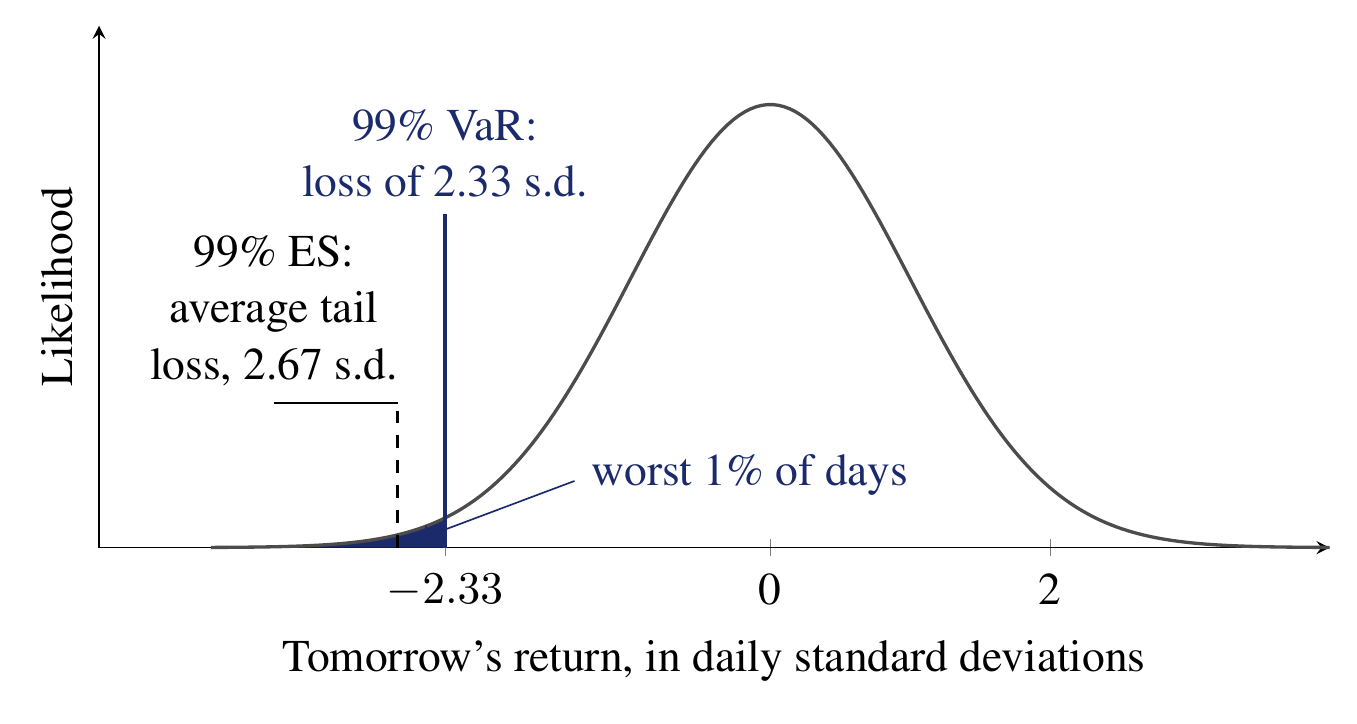
\includegraphics[width=0.85\linewidth]{images/fig13-1-var-es.png}
\caption{VaR and expected shortfall for normal returns. The 99\% VaR marks where the worst 1\% of days begins, 2.33 standard deviations below zero. The 99\% ES is the average loss within that tail, 2.67 standard deviations.}
\label{fig:13-var-es}
\end{figure}

\textbf{Coherence.} Artzner, Delbaen, Eber and Heath (1999) listed four properties a sensible risk measure should have. The one VaR can violate is \textbf{subadditivity}: the risk of a combined portfolio should not exceed the sum of the risks of its parts, since diversification should not add risk. ES is subadditive; VaR is not in general. VaR is subadditive for normal returns, so the failure shows up in portfolios with very skewed payoffs, such as credit and options.

\textbf{Square-root-of-time.} If daily returns are independent with the same variance, the $h$-day standard deviation is $\sqrt{h}$ times the daily one, so a 10-day VaR is about $\sqrt{10} \approx 3.16$ times the one-day VaR. Volatility clustering (Chapter 11) breaks the assumption: after a calm period the rule overstates risk, and after a shock it understates it.

\textbf{Methods.} The three main families of VaR models are set out in Section~\ref{sec:13-how}:

\begin{itemize}
  \item \emph{parametric}, which assumes a distribution and estimates $\sigma$;
  \item \emph{historical simulation}, which uses the empirical quantile of past returns;
  \item \emph{Monte Carlo}, which simulates from a model of the risk factors.
\end{itemize}

\textbf{Worked example.} A \$10 million position in a stock index has a daily volatility of 1.2\%.

\begin{itemize}
  \item Normal 99\% one-day VaR $= 2.326 \times 1.2\% \times \$10\text{m} \approx \$279{,}000$.
  \item Normal 99\% ES $= 1.2\% \times \phi(2.326)/0.01 \times \$10\text{m} = 2.665 \times 1.2\% \times \$10\text{m} \approx \$320{,}000$.
  \item Normal 97.5\% ES $= 2.338 \times 1.2\% \times \$10\text{m} \approx \$281{,}000$, almost the same as the 99\% VaR. This is why regulators chose 97.5\% when they moved from VaR to ES.
  \item 10-day VaR by the square-root rule: $\sqrt{10} \times \$279{,}000 \approx \$883{,}000$.
  \item With 500 days of history, the 99\% historical-simulation VaR is the loss between the 5th and 6th worst days.
\end{itemize}

\textbf{Subadditivity failure.} Two bonds each default with probability 4\%, losing 100 if they do and nothing otherwise. Each bond's 95\% VaR is 0, since default is less likely than 5\%. For a portfolio of both, with independent defaults, the probability of at least one default is $1 - 0.96^2 = 7.84\%$, so the portfolio's 95\% VaR is 100. Diversifying has \emph{increased} the measured risk.

\textbf{Further reading.} Hull, \emph{Risk Management and Financial Institutions} and \emph{Options, Futures, and Other Derivatives} (VaR and ES, historical simulation, model-building approach, backtesting); Jorion, \emph{Value at Risk: The New Benchmark for Managing Financial Risk}; McNeil, Frey and Embrechts, \emph{Quantitative Risk Management} (risk measures, coherence, backtesting); Christoffersen, \emph{Elements of Financial Risk Management} (VaR models and backtests).

\section{How it works}
\label{sec:13-how}

Every VaR model answers two questions: how volatile will tomorrow be, and what shape does the tail have? The models in this chapter combine different answers.

\begin{center}
\small
\begin{tabularx}{0.9\linewidth}{@{}>{\raggedright\arraybackslash}p{0.28\linewidth}>{\raggedright\arraybackslash}X>{\raggedright\arraybackslash}X@{}}
\toprule
Model & Volatility & Tail shape \\
\midrule
Normal, rolling window & Equal-weighted past window (here 250 days) & Normal \\
Historical simulation (HS) & Implicit in the window & Empirical quantile of past returns \\
EWMA (RiskMetrics) & Exponentially weighted, $\lambda = 0.94$ & Normal \\
GARCH & Estimated, mean-reverting & Normal \\
GJR-GARCH with Student-$t$ shocks & Estimated, with leverage effect & Student-$t$, estimated \\
Filtered historical simulation (FHS) & GJR-GARCH & Empirical quantile of past \emph{standardized} returns \\
\bottomrule
\end{tabularx}
\end{center}

\textbf{Historical simulation} is the most popular method at banks (P\'erignon and Smith 2010) because it needs no distributional assumption and handles nonlinear positions, such as options, by revaluing the portfolio under each past day's market moves. Its weakness is slowness. A 250-day window gives the same weight to a crash eleven months ago as to yesterday's, and none at all to one twelve months and a day ago. When volatility jumps, HS VaR responds only as the new large losses enter the window. When they leave, it drops abruptly.

\textbf{EWMA and GARCH} respond to volatility within days, which is Chapter 11's central finding. But with normal shocks they understate the tail. Even after volatility clustering is removed, standardized daily returns have fatter tails than the normal distribution, so a normal 99\% VaR built on a good volatility forecast is still breached too often.

\textbf{Filtered historical simulation} (Barone-Adesi, Giannopoulos and Vosper 1999; Hull and White 1998) combines the two strengths. It divides each past return by the volatility forecast for that day, giving standardized returns that are roughly independent and identically distributed. It takes their empirical quantile, which captures the fat tails without assuming a distribution, and multiplies by today's volatility forecast. The GJR-$t$ model does the same with a parametric tail.

A VaR model can fail in two distinct ways. It can be \textbf{wrong on average}, breached on 2\% of days instead of 1\%. Or it can be \textbf{right on average but wrong at the wrong times}, with breaches bunched in a few turbulent weeks. The second failure is the more dangerous, because the bunched breaches arrive exactly when capital is scarce. The backtests in Section~\ref{sec:13-backtest} test for both.

\section{The claim}
\label{sec:13-claim}

\begin{callout}
\textbf{Claim.} A well-built 99\% one-day VaR model is breached on about 1\% of trading days, and its breaches are independent over time. Breaches neither cluster in turbulent periods nor become more likely after a breach.
\end{callout}

This is the claim implicit in every VaR number a bank reports and in the Basel rules that used VaR to set capital. Christoffersen (1998) called the two parts \textbf{unconditional coverage} and \textbf{independence}. Together they form \textbf{conditional coverage}: on each day, given everything known the day before, the probability of a breach is exactly 1\%.

To test it we need to be precise on four points.

\begin{itemize}
  \item \textbf{Which models.} The claim is not that any VaR model works. It is that some models, built on the evidence of Chapter 11, can achieve conditional coverage. We test six, from the simplest to filtered historical simulation.
  \item \textbf{Which portfolio.} The lab uses the U.S. stock market, a single liquid position with daily data back to 1926. Bank portfolios are more complex, and their own backtests (Section~\ref{sec:13-evidence}) are the stronger test of practice.
  \item \textbf{Which confidence level.} The claim is stated at 99\%, the Basel level, but a model that is right at 99\% and badly wrong at 99.9\% is of limited use for the tail events that matter.
  \item \textbf{What would count against it.} The claim fails for a model if its breach rate differs significantly from 1\%, or if breaches are significantly clustered. It weakens if every model fails in crises, even those that pass over the full sample.
\end{itemize}

\section{The original evidence}
\label{sec:13-evidence}

\textbf{RiskMetrics and the Basel rules.} In 1994 J.P. Morgan published its RiskMetrics methodology and data free of charge. Its daily volatilities used the EWMA rule with $\lambda = 0.94$, and its VaR assumed normal returns. The fourth edition of the \emph{Technical Document} (1996) became the reference for the industry. In 1996 the Basel Committee allowed banks to use their own VaR models to set capital for market risk: a 99\% ten-day VaR, multiplied by at least 3. The multiplier rises with the number of breaches in a 250-day backtest, the \textbf{traffic light} described in Section~\ref{sec:13-backtest}. VaR thus became both a management tool and a regulatory one, and the backtest became a test with consequences.

\textbf{The statistics of backtesting.} Kupiec (1995) proposed testing whether the breach rate equals the stated probability, and showed how little power the test has over a single year: at 99\% only 2.5 breaches are expected in 250 days, so even a badly wrong model is hard to reject. Christoffersen (1998) added the test of independence and combined the two into the conditional-coverage test.

\textbf{Banks' own VaR.} Berkowitz and O'Brien (2002) obtained daily VaR forecasts and trading results for six large U.S. banks. The banks' 99\% VaRs were generally \emph{conservative}, breached less than 1\% of the time. But the breaches that did occur clustered, most of them in the turmoil of August to October 1998. A simple GARCH model of each bank's total trading P\&L performed about as well as the banks' detailed models and responded faster to changes in volatility. P\'erignon and Smith (2010) found that historical simulation was by far the most popular method among banks, and that historical-simulation VaR contained very little information about future volatility.

\textbf{Model comparisons.} Studies that backtest many models on index returns reach a consistent conclusion. Methods that combine a GARCH-type volatility forecast with a fat-tailed or empirical distribution of standardized returns perform best. Plain historical simulation and normal models with slow-moving volatility perform worst (Kuester, Mittnik and Paolella 2006). McNeil and Frey (2000) proposed the conditional extreme-value approach and the exceedance-residual test of expected shortfall used in this chapter's lab.

\section{Backtesting VaR and expected shortfall}
\label{sec:13-backtest}

A backtest compares each day's VaR forecast, made the day before, with that day's actual loss. A \textbf{breach} (or exception) is a day on which the loss exceeded the VaR. The breach sequence, a string of 0s and 1s, is the raw material for every test.

\textbf{Unconditional coverage (Kupiec 1995).} With $n$ days and $x$ breaches, the likelihood-ratio statistic compares the observed rate $x/n$ with the stated probability $\alpha$:
\begin{equation}
  LR_{uc} = -2\ln\!\left[(1 - \alpha)^{n-x}\,\alpha^{x}\right] + 2\ln\!\left[\left(1 - \tfrac{x}{n}\right)^{n-x}\left(\tfrac{x}{n}\right)^{x}\right]
  \label{eq:13-kupiec}
\end{equation}
Under the null hypothesis it has a $\chi^2$ distribution with one degree of freedom. It rejects both too many breaches (risk understated) and too few (capital wasted).

\textbf{Independence (Christoffersen 1998).} Estimate two probabilities: of a breach after a day without one ($\pi_{01}$), and of a breach after a breach ($\pi_{11}$). If breaches are independent, they are equal. The likelihood-ratio test of $\pi_{01} = \pi_{11}$ is $\chi^2(1)$. Adding $LR_{uc}$ gives the conditional-coverage test, $\chi^2(2)$. For a correct 99\% model, $\pi_{11}$ should be about 1\%. Values of 5\% to 10\% mean the model reacts too slowly to turbulence.

\textbf{The Basel traffic light.} Regulators count breaches of the 99\% one-day VaR over the most recent 250 trading days (Figure~\ref{fig:13-traffic}):

\begin{center}
\small
\begin{tabularx}{0.9\linewidth}{@{}>{\raggedright\arraybackslash}p{0.12\linewidth}>{\raggedright\arraybackslash}p{0.16\linewidth}>{\raggedright\arraybackslash}p{0.22\linewidth}>{\raggedright\arraybackslash}X@{}}
\toprule
Zone & Breaches & Capital multiplier & Probability of this many or fewer for a correct model \\
\midrule
Green & 0--4 & 3.0 & 89.2\% \\
Yellow & 5--9 & 3.40 to 3.85 & 99.99\% at 9 \\
Red & 10 or more & 4.0 & n/a \\
\bottomrule
\end{tabularx}
\end{center}

\begin{figure}[htbp]
\centering
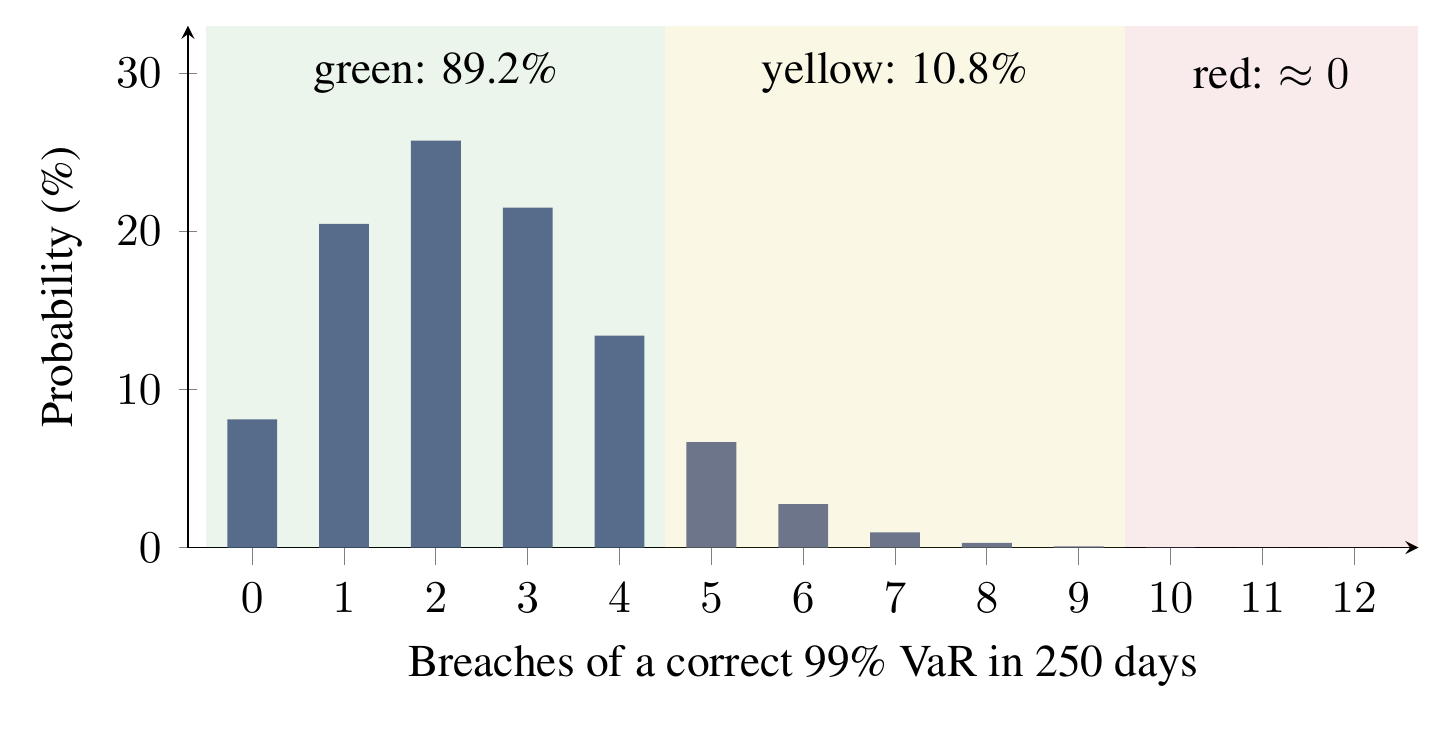
\includegraphics[width=0.85\linewidth]{images/fig13-2-traffic-light.png}
\caption{The Basel traffic light. The bars give the probability that a correct 99\% VaR model is breached a given number of times in 250 days. It lands in the green zone 89.2\% of the time and in the yellow zone 10.8\% of the time, and almost never in the red.}
\label{fig:13-traffic}
\end{figure}

A correct model lands in the yellow zone about one year in nine and almost never in the red. The zones were designed to balance two errors: penalizing banks with good models and letting banks with bad models through.

\textbf{Expected shortfall.} In 2016 the Basel Committee's Fundamental Review of the Trading Book replaced 99\% VaR with 97.5\% ES for setting market-risk capital, because ES captures the size of tail losses and is subadditive. ES is harder to backtest. Gneiting (2011) showed that ES, unlike VaR, is not \textbf{elicitable}: no scoring function is minimized by the true ES, so forecasts cannot be ranked by average loss as VaR forecasts can. Backtests exist nonetheless. The \textbf{exceedance-residual test} of McNeil and Frey (2000) checks whether, on breach days, the loss beyond the ES averages zero. Acerbi and Sz\'ekely (2014) proposed further tests. The Basel framework still backtests VaR at 97.5\% and 99\% alongside the ES used for capital.

\section{Replication lab: ninety-five years of VaR backtests}
\label{sec:13-lab}

\begin{callout}
\textbf{Lab 13 at a glance.} \emph{Claim on trial:} a well-built 99\% VaR model achieves conditional coverage. \emph{Data:} daily U.S. market returns (Mkt-RF + RF from the Kenneth French library) from 1930 to the present, about 24,000 trading days; free. \emph{Code:} runs as a script (\texttt{python lab13.py}) or as a notebook with a prediction prompt before each step.
\end{callout}

Lab 13 backtests the six models of Section~\ref{sec:13-how}. Every forecast uses only data up to the day before. The GARCH models are re-estimated once a year on the previous ten years.

\textbf{Part A, coverage.} For each model at 99\%: breaches against the roughly 240 expected, Kupiec and Christoffersen tests, average VaR, the worst loss as a multiple of the VaR, and the share of calendar years that would have fallen in the Basel yellow and red zones. Figure 13.3 shows two models through 2007--2010, and Figure 13.4 compares breach rates.

\textbf{Part B, clustering.} The probability of a breach after a breach, and breaches per year against the Basel zones (Figure 13.5).

\textbf{Part C, stress tests.} Breaches in four crises; the ratio of actual to expected breaches at confidence levels from 95\% to 99.9\% (Figure 13.6); and historical simulation with one, two and four years of data.

\textbf{Part D, expected shortfall.} At 97.5\%, the ratio of the average loss on breach days to the average ES forecast, and a test of whether exceedance residuals, scaled by volatility, average zero (Figure 13.7).

The lab tests the claim in its simplest setting: a single linear position in a liquid market with a long history. A bank's trading book adds options, credit and illiquid positions, and those make every model harder to build. If the models struggle here, they will not do better there.

\textbf{What the simulated run shows.} The simulation draws returns from a GJR-GARCH model with Student-$t$ shocks, so the GJR-$t$ model is the true model. It passes every test: 1.01\% breaches at 99\%, a breach probability after a breach of 0.8\%, and an ES ratio of 1.00. Filtered historical simulation is nearly as good. The normal and historical-simulation models are breached about twice as often as they should be, with strong clustering, and they understate ES. These results confirm that the code and the tests work. They say nothing about real markets. Run the lab on the real data to reach your own verdict.

\section{Stress tests}
\label{sec:13-stress}

\textbf{Crises.} The full-sample breach rate can hide disastrous weeks. On October 19, 1987, the Dow Jones Industrial Average fell 22.6\%, its largest one-day percentage loss. No model calibrated on the calm months before could have put that inside a 99\% VaR. Part C counts breaches in 1930--32, October 1987, the autumn of 2008 and the spring of 2020. A correct 99\% model should average about 0.2 breaches in a 22-day month. Expect every model to exceed that in these windows. The question is how many breaches each produces and how quickly it adapts.

\textbf{Confidence level.} Fat tails punish models more the further into the tail they go. Under the normal distribution a 99.9\% loss is only 1.33 times a 99\% loss ($3.09/2.33$). In equity returns the ratio is larger. Normal-based models that are slightly off at 95\% can be several times off at 99.9\% (Figure 13.6). The test also has very little power at 99.9\%: about 24 breaches are expected in 95 years, so a single bad week moves the ratio noticeably.

\textbf{Window length.} A short historical-simulation window adapts faster but estimates the 1\% quantile from very few observations: with 250 days, only two or three. A long window is more stable but slower to react after a calm period. Part C compares 250, 500 and 1,000 days. The choice moves the breach rate but does not fix clustering, since no equal-weighted window responds to volatility the way GARCH does.

\textbf{Procyclicality.} A VaR that responds quickly to volatility, as GARCH and EWMA do, raises capital requirements and forces deleveraging in exactly the weeks when markets are falling. That is good risk measurement but can amplify a crisis if every bank does it at once. A slow VaR, such as long-window historical simulation, is less procyclical but is breached in clusters. Basel 2.5 (2009) added a \textbf{stressed VaR}, calibrated to a year of significant stress, partly to make capital less dependent on recent calm.

\section{Verdict}
\label{sec:13-verdict}

\begin{callout}
\textbf{Verdict: weakens} (as of October 2026). The claim holds for the right models in normal times: VaR models that combine a responsive volatility forecast with a fat-tailed distribution come close to 1\% breaches at 99\% with little clustering over long samples. It fails for the models most widely used in practice, normal and plain historical simulation, which are breached in clusters. It fails for every model in the first days of a crisis and deep in the tail.
\end{callout}

What survives:

\begin{itemize}
  \item \textbf{Coverage is achievable.} Filtered historical simulation and GARCH models with fat-tailed shocks deliver close to the stated breach rate over long samples, in the literature and in tests like the lab's. The tools of Chapter 11 work.
  \item \textbf{Backtesting works as designed.} The Kupiec and Christoffersen tests, and the Basel traffic light, separate good models from bad ones over long samples. A model that clusters its breaches is caught.
\end{itemize}

What weakens it:

\begin{itemize}
  \item \textbf{Practice lags the evidence.} Historical simulation, the most popular method at banks, reacts slowly and contains little information about future volatility (P\'erignon and Smith 2010). Its breaches cluster in exactly the periods when losses matter.
  \item \textbf{Crises break every model.} No model built on past data anticipates the first day of a crash. In October 1987, in 2008 and in March 2020 breaches came in bunches.
  \item \textbf{The tail beyond 99\% is poorly measured.} Breach rates at 99.9\% are worse for most models, and the tests have little power to tell.
  \item \textbf{VaR says nothing about the size of the loss beyond it.} A model can pass every VaR backtest while understating how bad the bad days are. Expected shortfall addresses this, but it inherits the same volatility forecasts and is harder to backtest.
\end{itemize}

The verdict would move to \emph{survives} if the models used in practice achieved conditional coverage through crises, which would require volatility forecasts faster than any yet built from daily data. It would move to \emph{fails} if even the best models failed coverage tests over long samples, which the evidence so far does not show.

\section{What practitioners and investors can use}
\label{sec:13-investors}

\textbf{For anyone measuring risk:}

\begin{itemize}
  \item \textbf{Use a responsive volatility forecast.} EWMA at the least, GARCH-type models for better results. A one-year equal-weighted window is too slow.
  \item \textbf{Use fat tails.} Scale standardized returns by an empirical or Student-$t$ distribution rather than the normal. Filtered historical simulation does both and is easy to implement.
  \item \textbf{Report ES alongside VaR,} and look at the largest losses directly, not only at percentiles.
  \item \textbf{Backtest continuously.} Count breaches, and also check whether they cluster. A model with the right number of breaches all in one month is not a good model.
  \item \textbf{Stress test separately.} VaR describes ordinary bad days. Scenarios such as a repeat of October 1987, 2008 or 2022 describe the days that threaten survival, and no backtest on recent data covers them.
\end{itemize}

\textbf{For investors reading a bank's or fund's risk disclosures:}

\begin{itemize}
  \item What method produces the VaR, and over what window? A historical simulation with a one-year window will look reassuring after a calm year.
  \item How many backtesting exceptions were there last year, and when did they occur?
  \item What is the stressed VaR or the worst scenario loss, relative to the reported VaR?
  \item What positions are hard to value daily? Their risk may not appear in the VaR at all.
\end{itemize}

\begin{callout}
\textbf{What Failed: bank VaR in 2007--08.} By 2007 large banks' trading risk was measured mainly by VaR and stress tests, and their market-risk capital was based on VaR. The Swiss Federal Banking Commission's investigation of UBS, the bank with the largest subprime losses in Europe, found that its super-senior CDO tranches had been judged ``VaR neutral,'' so they ``were not reflected in key internal risk reports.'' The AAA ratings fed straight into the risk metrics. Risk models, including VaR, ``operated on the basis of overoptimistic assumptions,'' and stress scenarios were ``too optimistic'': ``The real shocks proved to be far greater than any shocks anticipated.'' UBS's own report to shareholders recorded that the super-senior positions, which the desk had treated as fully hedged with protection on only a small part of their value, accounted for about half of the bank's losses by the end of 2007.

The failure was not that VaR was computed wrongly. It was that VaR measured the risk of positions that looked safe in recent data and could not see the risk of a market that had never been stressed. The regulatory response was the stressed VaR of Basel 2.5 and, later, the move to expected shortfall. In March 2020, regulators faced the opposite problem: banks' backtesting exceptions jumped with market volatility, and the Federal Reserve and other U.S. agencies excluded exceptions from March 6 to March 27, 2020, from the count, judging that they reflected ``widespread and unusual volatility'' (Board of Governors of the Federal Reserve System 2021).
\end{callout}

\section{Open questions}
\label{sec:13-open}

\begin{itemize}
  \item \textbf{Can intraday data fix the first day of a crisis?} Realized volatility from intraday returns (Chapter 11) responds faster than daily GARCH. Does it reduce breach clustering at the onset of crises?
  \item \textbf{How should ES be backtested and compared?} ES is not elicitable on its own, but it is jointly elicitable with VaR. Which tests have power at the sample sizes banks actually have?
  \item \textbf{Is risk measurement procyclical by design?} A VaR that responds quickly forces deleveraging in falling markets. How should risk measures balance accuracy against stability?
  \item \textbf{What about portfolios VaR handles badly?} Options, credit and illiquid assets have nonlinear or stale prices. How much worse are VaR backtests for them, and what replaces VaR there?
\end{itemize}

\section*{Exercises}
\addcontentsline{toc}{section}{Exercises}

\subsection*{Conceptual (all readers)}

\begin{enumerate}
  \item A \$5 million position has a daily volatility of 1.5\%. Compute the normal 95\% and 99\% one-day VaR, the 99\% ES and the 10-day 99\% VaR by the square-root rule.
  \item Using the two-bond example in Section~\ref{sec:13-foundations}, compute the portfolio's 95\% ES and show that ES is subadditive in this case.
  \item A bank reports 7 breaches of its 99\% VaR in 250 days. Compute the Kupiec statistic and p-value. Which Basel zone is it in, and what is the capital multiplier?
\end{enumerate}

\subsection*{Lab extensions (technical readers)}

\begin{enumerate}
  \setcounter{enumi}{3}
  \item Part A: which models pass the Kupiec test at 99\%? Which pass the Christoffersen independence test? Is there a model that passes one but not the other?
  \item Part B: for historical simulation, compute the average number of days between breaches and compare it with the 100 days expected. What does the distribution of durations tell you?
  \item Part C: count each model's breaches in October 1987. How many days did each model take before its VaR exceeded the losses of the following days?
  \item Part C: rerun the backtest at 99.9\%. Which models are within a factor of two of the expected breach rate? How confident can you be, given the number of breaches expected?
  \item Part D: do the models that pass the VaR backtest also pass the ES backtest? Is there a model that passes VaR but fails ES?
  \item A regulator proposes requiring all banks to use filtered historical simulation. Using the evidence in this chapter, write the case for and against, including the effect on procyclicality.
\end{enumerate}

\section*{References}
\addcontentsline{toc}{section}{References}

\begin{itemize}
  \item Acerbi, C. and Sz\'ekely, B. (2014). Back-Testing Expected Shortfall. \emph{Risk}, December 2014.
  \item Artzner, P., Delbaen, F., Eber, J.-M. and Heath, D. (1999). Coherent Measures of Risk. \emph{Mathematical Finance} 9(3): 203--228.
  \item Barone-Adesi, G., Giannopoulos, K. and Vosper, L. (1999). VaR without Correlations for Portfolios of Derivative Securities. \emph{Journal of Futures Markets} 19(5): 583--602.
  \item Basel Committee on Banking Supervision (1996). \emph{Supervisory Framework for the Use of ``Backtesting'' in Conjunction with the Internal Models Approach to Market Risk Capital Requirements}. Basel: Bank for International Settlements.
  \item Basel Committee on Banking Supervision (2009). \emph{Revisions to the Basel II Market Risk Framework}. Basel: Bank for International Settlements.
  \item Basel Committee on Banking Supervision (2016). \emph{Minimum Capital Requirements for Market Risk}. Basel: Bank for International Settlements.
  \item Berkowitz, J. and O'Brien, J. (2002). How Accurate Are Value-at-Risk Models at Commercial Banks? \emph{Journal of Finance} 57(3): 1093--1111.
  \item Board of Governors of the Federal Reserve System (2021). Banks' Backtesting Exceptions during the COVID-19 Crash: Causes and Consequences. \emph{FEDS Notes}, July 8.
  \item Christoffersen, P. F. (1998). Evaluating Interval Forecasts. \emph{International Economic Review} 39(4): 841--862.
  \item Gneiting, T. (2011). Making and Evaluating Point Forecasts. \emph{Journal of the American Statistical Association} 106(494): 746--762.
  \item Hull, J. and White, A. (1998). Incorporating Volatility Updating into the Historical Simulation Method for Value-at-Risk. \emph{Journal of Risk} 1(1): 5--19.
  \item J.P. Morgan/Reuters (1996). \emph{RiskMetrics---Technical Document} (4th ed.). New York: Morgan Guaranty Trust Company.
  \item Kuester, K., Mittnik, S. and Paolella, M. S. (2006). Value-at-Risk Prediction: A Comparison of Alternative Strategies. \emph{Journal of Financial Econometrics} 4(1): 53--89.
  \item Kupiec, P. H. (1995). Techniques for Verifying the Accuracy of Risk Measurement Models. \emph{Journal of Derivatives} 3(2): 73--84.
  \item McNeil, A. J. and Frey, R. (2000). Estimation of Tail-Related Risk Measures for Heteroscedastic Financial Time Series: An Extreme Value Approach. \emph{Journal of Empirical Finance} 7(3--4): 271--300.
  \item P\'erignon, C. and Smith, D. R. (2010). The Level and Quality of Value-at-Risk Disclosure by Commercial Banks. \emph{Journal of Banking \& Finance} 34(2): 362--377.
  \item Swiss Federal Banking Commission (2008). \emph{Subprime Crisis: SFBC Investigation into the Causes of the Write-downs of UBS AG}. Bern: SFBC.
  \item UBS AG (2008). \emph{Shareholder Report on UBS's Write-Downs}. Zurich: UBS.
\end{itemize}

\textbf{Data:} Kenneth R. French Data Library, Fama/French 3 Factors [Daily].

% Chapter 14 -- Claim: Selling Options Earns a Reliable Premium
% Requires: amsmath, amssymb, booktabs, array, tabularx, graphicx, tcolorbox (breakable, skins), hyperref or url.
% Defines the callout box only if the preamble has not.
\providecolor{fenavy}{HTML}{1B2A6B}
\providecolor{feshade}{HTML}{F3F5FA}
\makeatletter
\@ifundefined{callout}{%
  \newtcolorbox{callout}{breakable, enhanced,
    colback=white, colframe=gray!70, boxrule=0.5pt, arc=1mm,
    borderline west={2.5pt}{0pt}{gray!70},
    left=8pt, right=8pt, top=4pt, bottom=4pt}%
}{}
\makeatother

\chapter{Claim: Selling Options Earns a Reliable Premium}
\label{ch:14}

An insurance company collects premiums every month and pays out claims now and then. If it prices its policies a little above expected claims, it earns a steady profit, with the occasional very bad year when a hurricane hits. An investor who sells stock-index options is in the same business. A put option is insurance against a market fall. Its seller collects a premium up front and pays out when the market drops.

The claim in this chapter is that this insurance is systematically overpriced: option prices imply more volatility than the market goes on to deliver, so sellers earn a premium. It is one of the best-documented facts in derivatives markets, and it underpins a large industry of option-income funds, covered-call ETFs and volatility-selling strategies.

The question is what kind of premium it is. A reliable premium for bearing a risk that others want to shed is one thing. A strategy that wins small most months and loses large in a few, while carrying most of the stock market's risk, is another. The two can look alike in a backtest, and the evidence has to separate them.

By the end of the chapter you will be able to:

\begin{itemize}
  \item describe call and put payoffs and use put--call parity to show that a covered call and a cash-secured put are the same position;
  \item price an option by Black--Scholes, compute its Greeks, and back out implied volatility;
  \item define the VIX and the variance risk premium, and estimate a seller's expected gain from the gap between implied and realized volatility;
  \item state the claim that selling options earns a reliable premium, and separate the variance risk premium from the returns of option-income strategies;
  \item measure option-strategy performance with beta-matched benchmarks, up and down betas and the manipulation-proof performance measure;
  \item judge what an option-income fund is likely to deliver, and what can go wrong.
\end{itemize}

\section{Foundations: options, Black--Scholes and implied volatility}
\label{sec:14-foundations}

\textbf{Payoffs.} A \textbf{call} gives the right to buy an asset at the \textbf{strike price} $K$ on the expiry date $T$; at expiry it pays $\max(S_T - K, 0)$, where $S_T$ is the asset's price then. A \textbf{put} gives the right to sell; it pays $\max(K - S_T, 0)$. An option is \textbf{at the money} when $K$ equals the current price, \textbf{out of the money} when exercising now would pay nothing (a put with $K$ below $S$), and \textbf{in the money} otherwise. The buyer pays a \textbf{premium}; the seller (or \textbf{writer}) receives it and takes on the obligation.

\textbf{Put--call parity.} For European options, which can be exercised only at expiry, on a non-dividend-paying asset with the same strike and expiry:
\begin{equation}
  C - P = S - K e^{-rT}
  \label{eq:14-parity}
\end{equation}
Rearranged, \emph{stock plus a short call} equals \emph{cash of $Ke^{-rT}$ plus a short put}. A \textbf{covered call} (own the stock, sell a call) and a \textbf{cash-secured put} (hold the strike in bills, sell a put) with the same strike are the same position.

\textbf{Black--Scholes--Merton.} If the stock follows a geometric Brownian motion with constant volatility $\sigma$, an option can be replicated by trading the stock and a bond, so its price does not depend on investors' risk preferences (Black and Scholes 1973; Merton 1973):
\begin{equation}
  C = S\,N(d_1) - K e^{-rT} N(d_2), \qquad P = K e^{-rT} N(-d_2) - S\,N(-d_1)
  \label{eq:14-bs}
\end{equation}
\begin{equation}
  d_1 = \frac{\ln(S/K) + (r + \sigma^2/2)\,T}{\sigma\sqrt{T}}, \qquad d_2 = d_1 - \sigma\sqrt{T}
  \label{eq:14-d}
\end{equation}
where $N$ is the standard normal distribution function. Chapter 15 tests the replication argument itself.

\textbf{The Greeks} measure sensitivities.

\begin{itemize}
  \item \textbf{Delta} ($\partial V/\partial S$) is the number of shares that hedge the option: $N(d_1)$ for a call, $N(d_1) - 1$ for a put.
  \item \textbf{Gamma} is the change in delta as $S$ moves.
  \item \textbf{Vega} is the change in price per unit change in $\sigma$.
  \item \textbf{Theta} is the change in price as time passes.
\end{itemize}

An option seller is short gamma and short vega, and collects theta: time decay works in the seller's favour, large moves against.

\textbf{Implied volatility} is the $\sigma$ that makes the Black--Scholes price equal the market price. It is the market's price of volatility, not a forecast in the statistical sense. \textbf{Realized volatility} is the standard deviation of returns that actually occurs over the option's life. Implied volatility differs across strikes: for stock indexes, out-of-the-money puts trade at higher implied volatilities than at-the-money options, a pattern called the \textbf{skew} (Chapter 15).

\textbf{The VIX} is Cboe's index of 30-day implied volatility for the S\&P 500, computed from a strip of out-of-the-money calls and puts. Its square approximates the fair strike of a 30-day \textbf{variance swap}, a contract that pays the difference between realized variance and a fixed strike. The \textbf{variance risk premium} is the expected difference between implied (risk-neutral) variance and realized variance.

\textbf{Worked example.} The index is at 100, the risk-free rate is 4\%, and a one-month at-the-money put trades at an implied volatility of 20\%.

\begin{itemize}
  \item Black--Scholes price: $P = \$2.14$ per \$100 of index. The call is worth \$2.47; the difference, \$0.33, equals $100 - 100\,e^{-0.04/12}$, as parity requires.
  \item Suppose volatility over the month turns out to be 16\%. At 16\%, the put would have been worth \$1.68. The seller's expected gain is roughly $\$2.14 - \$1.68 = \$0.46$, or vega (\$0.115 per vol point) times the 4-point gap.
  \item That is an \emph{expected} gain. If the index falls 10\% during the month, the put pays \$10 and the seller loses $\$10 - \$2.14 = \$7.86$, about seventeen months of expected gains at \$0.46 a month (Figure~\ref{fig:14-put}).
\end{itemize}

\begin{figure}[htbp]
\centering
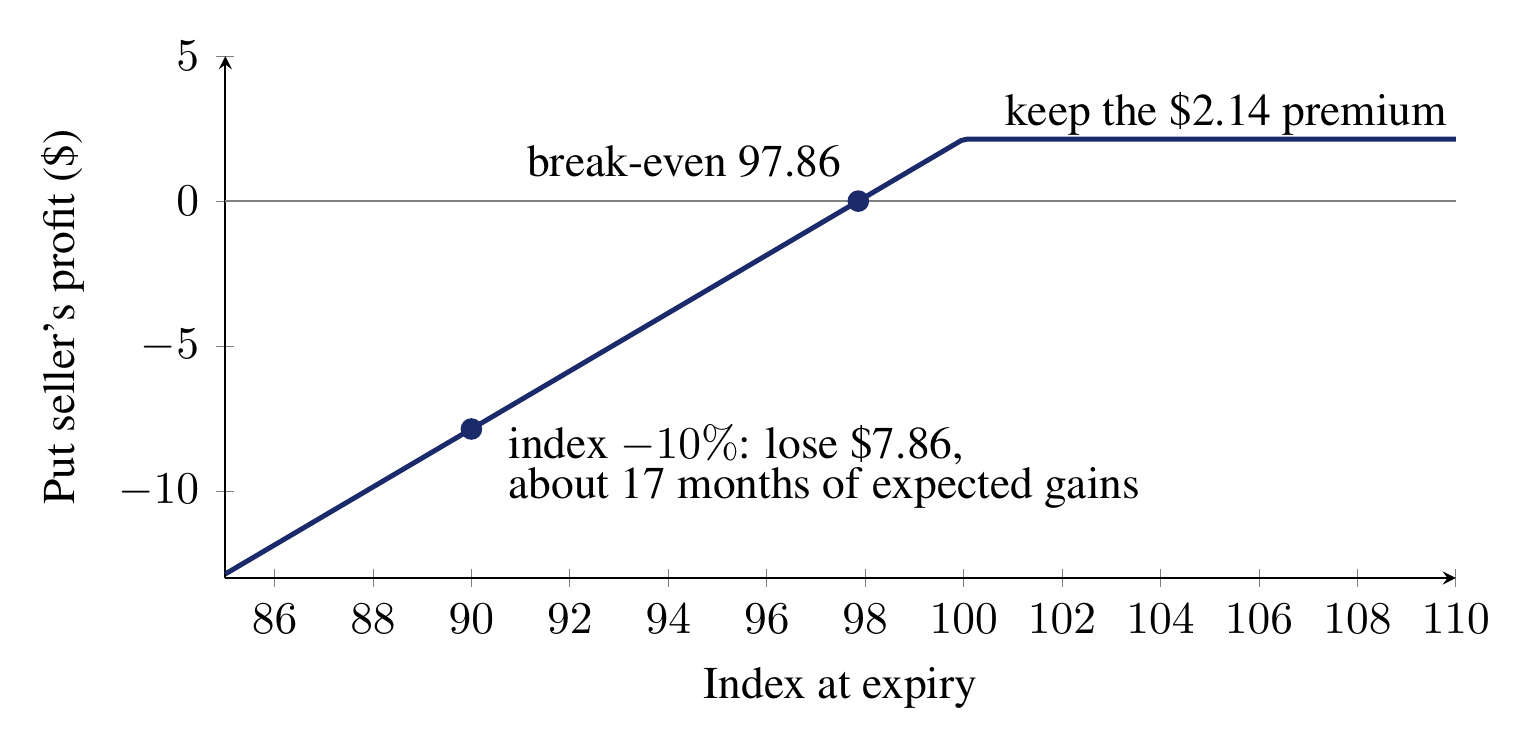
\includegraphics[width=0.85\linewidth]{images/fig14-1-short-put.png}
\caption{The put seller's profit at expiry in the worked example. Above the strike of 100 the seller keeps the \$2.14 premium; below the break-even of 97.86 the loss grows one for one with the fall. A 10\% fall costs \$7.86, about seventeen months of expected gains.}
\label{fig:14-put}
\end{figure}

\textbf{Further reading.} Hull, \emph{Options, Futures, and Other Derivatives} (option properties, put--call parity, Black--Scholes--Merton, the Greeks, volatility smiles, variance swaps); Natenberg, \emph{Option Volatility and Pricing}; Bodie, Kane and Marcus, \emph{Investments} (option strategies); Gatheral, \emph{The Volatility Surface}.

\section{How it works}
\label{sec:14-how}

\textbf{Why insurance might be overpriced.} Many investors hold stock portfolios they cannot easily sell and want protection against crashes. Pension funds, insurers and structured-product issuers buy index puts; market makers who sell them must hold capital against the risk and cannot fully hedge it. Bollen and Whaley (2004) and G\^arleanu, Pedersen and Poteshman (2009) showed that this net buying pressure raises option prices, especially for out-of-the-money puts. In equilibrium, sellers are paid for bearing a risk that bites in the worst states of the world, when investors' wealth is low and losses hurt most. A premium for that risk is not a free lunch. It is compensation, and it should be large precisely because the losses come at bad times.

\textbf{Ways to sell volatility.} The strategies differ in how much equity risk they carry alongside the volatility exposure.

\begin{center}
\small
\begin{tabularx}{0.9\linewidth}{@{}>{\raggedright\arraybackslash}p{0.19\linewidth}>{\raggedright\arraybackslash}X>{\raggedright\arraybackslash}X>{\raggedright\arraybackslash}X@{}}
\toprule
Strategy & Position & Equity exposure & Main risk \\
\midrule
Covered call (buy-write) & Own the index, sell a call & High (beta about 0.5--0.8) & Market falls; gains capped in rallies \\
Cash-secured put (put-write) & Hold bills, sell a put & High (same as covered call at the same strike) & Market falls \\
Short straddle & Sell a call and a put & Low on average, changes with the market & Large moves either way \\
Delta-hedged option & Sell an option, hedge its delta daily & Near zero & Realized volatility above implied \\
Short variance swap & Receive fixed variance, pay realized & Near zero, but crashes raise realized variance & Volatility spikes \\
\bottomrule
\end{tabularx}
\end{center}

The first two are what most retail and institutional ``option income'' products do. The last two isolate the variance risk premium itself. Comparing them is the heart of this chapter: if the covered call's return is mostly the equity premium earned with a beta of 0.6, it is not evidence that selling options pays.

\textbf{The payoff shape.} A covered call keeps the downside of the stock market but caps the upside at the strike plus the premium (Figure~\ref{fig:14-cc}). In calm or gently rising months it beats the market; in strong rallies it lags; in crashes it loses almost as much as the market, cushioned only by the premium. The return distribution is therefore \textbf{negatively skewed}. Most months bring small gains, and a few bring large losses.

\begin{figure}[htbp]
\centering
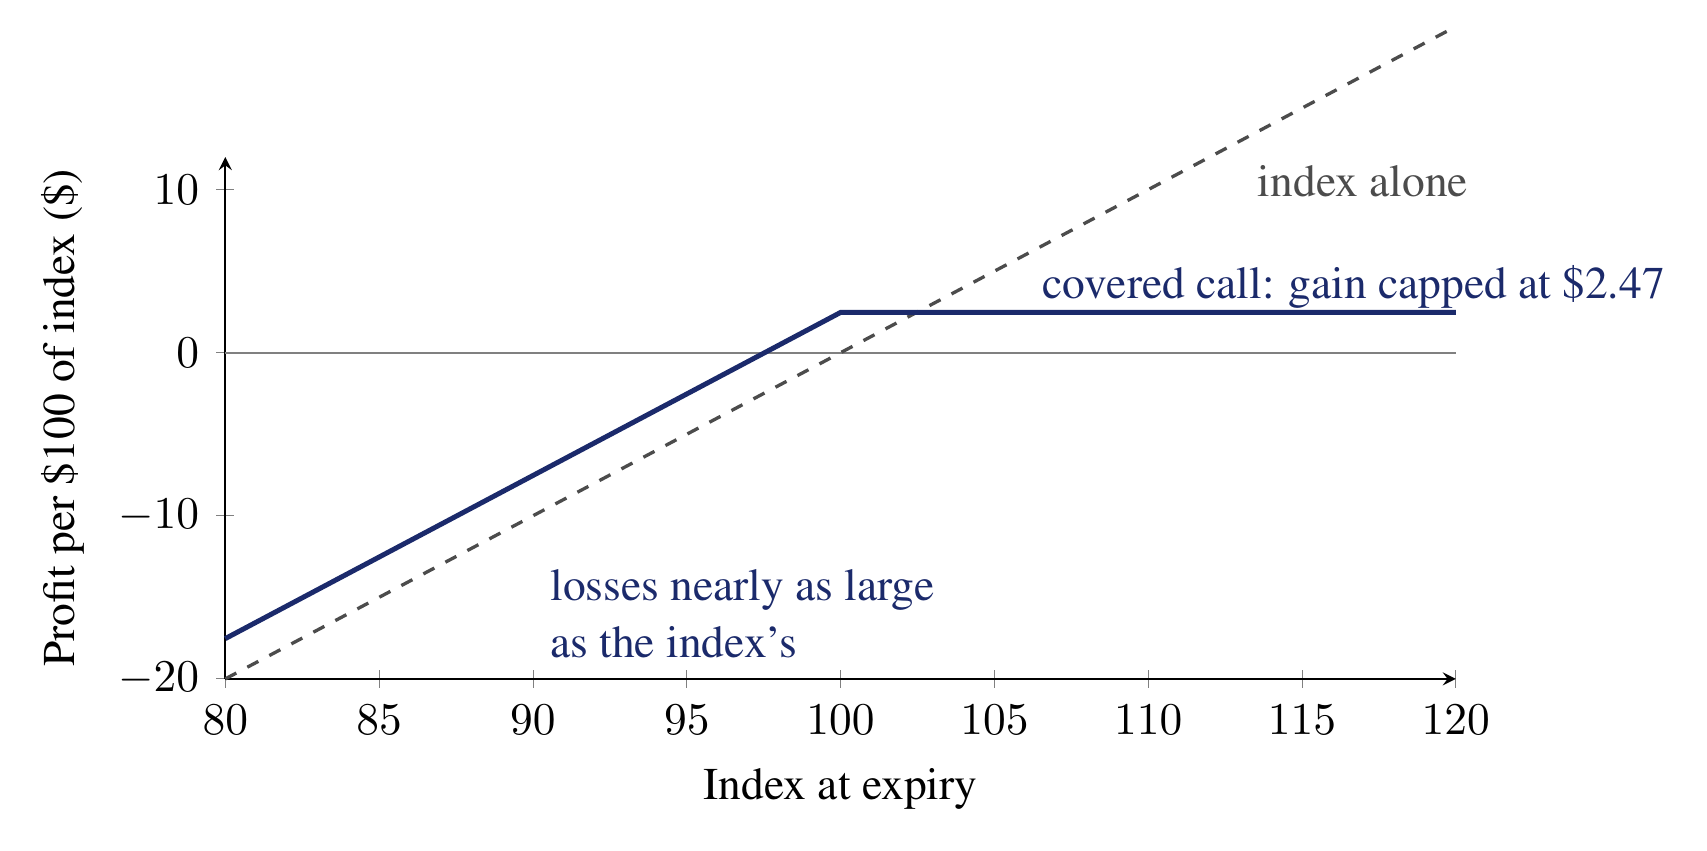
\includegraphics[width=0.85\linewidth]{images/fig14-2-covered-call.png}
\caption{A one-month at-the-money covered call against the index alone, using the worked example's prices. The call premium of \$2.47 caps the gain and cushions the loss by the same amount, so the covered call keeps almost all of the index's downside.}
\label{fig:14-cc}
\end{figure}

That shape creates a measurement problem. The Sharpe ratio uses only the mean and standard deviation, so it cannot see skewness. Selling out-of-the-money options can raise a portfolio's Sharpe ratio while making its tail much worse. Section~\ref{sec:14-measure} sets out measures that are harder to game.

\section{The claim}
\label{sec:14-claim}

\begin{callout}
\textbf{Claim.} Implied volatility exceeds the volatility that follows, on average, so option sellers earn a reliable premium. Strategies that sell index options, such as covered calls and put-writing, deliver better risk-adjusted returns than holding the index.
\end{callout}

The claim has two parts that can succeed or fail separately.

\begin{itemize}
  \item \textbf{The variance risk premium.} Implied variance is, on average, above the realized variance that follows. This is a statement about prices and can be tested directly by comparing the VIX with subsequent realized volatility.
  \item \textbf{The strategy premium.} Covered-call and put-writing strategies earn more than their risk justifies. This requires the variance premium to survive trading costs, early exercise and roll timing, and it requires an honest risk adjustment.
\end{itemize}

To test it we need to be precise on three points.

\begin{itemize}
  \item \textbf{What counts as risk.} A strategy with a beta of 0.5 should be compared with half the market plus half in bills, not with the whole market. Its negative skewness should be priced, not ignored.
  \item \textbf{What counts as reliable.} A premium that is positive in most months but wiped out in a few is reliable in one sense and not in another. We report both the share of months positive and the size of the worst losses.
  \item \textbf{What would count against it.} The variance risk premium fails if implied volatility is not significantly above realized volatility on average. The strategy claim fails if covered calls and put-writing earn no alpha after adjusting for beta, or if their advantage disappears once skewness is priced.
\end{itemize}

\section{The original evidence}
\label{sec:14-evidence}

\textbf{Option returns.} Coval and Shumway (2001) studied S\&P 500 index options and found that buying zero-beta, at-the-money \textbf{straddles} (a call and a put at the same strike) lost about 3\% a week on average. A straddle has little exposure to the direction of the market, so its losses point to a price for volatility itself. Bakshi and Kapadia (2003) found that delta-hedged option positions lost money on average, and attributed the losses to a negative market volatility risk premium: investors pay to be long volatility because volatility rises when markets fall.

\textbf{The variance risk premium.} Carr and Wu (2009) showed how to compute the variance swap rate from a portfolio of options, the method behind today's VIX, and used it to measure the premium directly for five stock indexes and 35 individual stocks. For the S\&P 500, implied variance was well above realized variance on average. Bollerslev, Tauchen and Zhou (2009) found that the size of the premium also predicts stock-market returns at a quarterly horizon, better than the price--earnings ratio or the default spread, consistent with its being a price of economic uncertainty.

\textbf{Covered calls and put-writing.} Cboe commissioned Robert Whaley to design the BuyWrite Index (BXM), which tracks an S\&P 500 portfolio that sells a one-month, near-the-money call each month. Whaley (2002) found that it had earned returns close to the S\&P 500's with substantially lower volatility. A later study for Cboe (Callan Associates 2006) reported that from June 1988 to August 2006 the BXM returned 11.77\% a year against 11.67\% for the S\&P 500, with a standard deviation of 9.29\% against 13.89\%. Cboe later added a PutWrite Index (PUT), which sells one-month at-the-money puts against Treasury-bill collateral. These results drew large inflows into option-income products.

\textbf{The skeptics.} Broadie, Chernov and Johannes (2009) argued that large average losses on index puts are not by themselves evidence of mispricing. Under standard models with jumps and reasonable risk premiums, put returns are expected to be very negative and very noisy, so short samples say little. Israelov and Nielsen (2015) decomposed covered-call returns into three exposures: the equity market, short volatility and an unintended equity reversal bet. Equity exposure drove most of the risk and return. The short-volatility component had a Sharpe ratio near 1.0 but contributed less than 10\% of the risk, and the reversal component added about a quarter of the risk with little return. A covered call, in other words, is mostly a stock-market position.

\section{Measuring option-strategy returns}
\label{sec:14-measure}

Option-selling strategies are the textbook case where the usual performance measures mislead. Four corrections matter.

\textbf{Adjust for beta.} A covered call with a beta of 0.6 should earn about 60\% of the equity premium without any volatility premium at all. The relevant comparison is a \textbf{beta-matched} portfolio, 60\% in the market and 40\% in bills, or equivalently the CAPM alpha (Chapter 12). A covered call that matches the market's return with two-thirds of its volatility may have earned no alpha.

\textbf{Look at both betas.} Selling options makes exposure asymmetric. The \textbf{down beta}, estimated in months when the market falls, is close to 1: the strategy takes most of the loss. The \textbf{up beta}, estimated in rising months, is much lower, because the call caps the gains. An investor who cares about losses more than gains should weigh the down beta.

\textbf{Price the skewness.} The Sharpe ratio ignores skewness, so a strategy can raise it by selling crash insurance. Goetzmann, Ingersoll, Spiegel and Welch (2007) showed that a manager can raise a portfolio's Sharpe ratio by selling out-of-the-money options, without any skill. They proposed a \textbf{manipulation-proof performance measure (MPPM)}:
\begin{equation}
  \Theta = \frac{1}{(1 - \rho)\,\Delta t}\,\ln\!\left\{\frac{1}{T}\sum_{t=1}^{T}\left[\frac{1 + r_t}{1 + r_{f,t}}\right]^{1-\rho}\right\}
  \label{eq:14-mppm}
\end{equation}
Here $T$ is the number of periods, $\Delta t$ the length of each period in years, and $r_t$ and $r_{f,t}$ the strategy's and the risk-free return. $\Theta$ is the certainty-equivalent excess return of an investor with constant relative risk aversion $\rho$. With $\rho = 3$, a typical value, a large negative month costs far more than a large positive month gains, so selling crash insurance cannot improve the score unless it really adds value.

\textbf{Respect the sample.} A strategy that loses heavily once a decade needs several decades of data to estimate its mean (Section~\ref{sec:03-se}). Broadie, Chernov and Johannes (2009) showed how noisy put returns are even over twenty years. A backtest that starts after 2009 and ends before 2020, for example, would miss both of the big losses of the period since 1990.

\section{Replication lab: the VIX, put-writing and covered calls since 1990}
\label{sec:14-lab}

\begin{callout}
\textbf{Lab 14 at a glance.} \emph{Claim on trial:} selling index options earns a reliable premium. \emph{Data:} daily market returns from the Kenneth French library and the VIX from FRED, which starts in 1990; both are free. Cboe's PUT and BXM index histories can be added for comparison. \emph{Code:} runs as a script (\texttt{python lab14.py}) or as a notebook with a prediction prompt before each step.
\end{callout}

\textbf{Part A, the variance risk premium.} At each month end, the VIX is compared with the market's realized volatility over the next 21 trading days. The lab reports the average gap in volatility points with a Newey--West $t$-statistic, the share of months in which implied exceeded realized, the median gap and the worst months (Figures 14.3 and 14.4).

\textbf{Part B, strategies.} The lab rebuilds two strategies from the data. Each month it sells a one-month option priced by Black--Scholes at the VIX and holds it to the next month end:

\begin{itemize}
  \item an \textbf{at-the-money put-write}, collateralized by bills like Cboe's PUT. By put--call parity this is also an at-the-money covered call, and the lab checks that the two returns are identical;
  \item a \textbf{covered call 2\% out of the money}, which keeps more of the market's upside.
\end{itemize}

Each is compared with the market on excess return, volatility, Sharpe ratio, skewness, worst month, drawdown, beta and CAPM alpha, over its own history and over a common period (Figure 14.5).

\textbf{Part C, stress tests.} Returns in crisis periods, the five worst market months, up and down betas, and the MPPM (Figure 14.6).

\textbf{Part D, equity versus volatility.} Each strategy's excess return is split into the part explained by beta and the alpha that remains. The lab compares it with the market scaled to the same beta, and with a pure short variance swap struck at VIX$^2$, sized to 10\% annual volatility (Figure 14.7).

The rebuilt strategies are deliberately simple, and that matters for interpretation. They price options at the VIX, which includes the premium on out-of-the-money puts and so usually exceeds at-the-money implied volatility. That overstates the premium a seller actually collects. They also ignore bid--ask spreads and roll at month ends rather than on Cboe's third-Friday schedule. The \texttt{-{}-iv-shift} option prices the options a few points below the VIX. Comparing the rebuilt series with Cboe's indices, which use traded prices, shows how much these simplifications matter.

\textbf{What the simulated run shows.} The simulation builds in a VIX 12\% above expected volatility. The lab finds the premium (implied above realized in 83\% of months), a put-write with a beta of about 0.5, strongly negative skewness and a down beta near 0.9 against an up beta near 0.15. The rebuilt put-write and covered call show positive alphas when options are priced at the inflated VIX. The Cboe-like series, priced 2 points lower, show none. These results confirm that the code works. They say nothing about real markets. Run the lab on the real data to reach your own verdict.

\section{Stress tests}
\label{sec:14-stress}

\textbf{Crashes.} The months that decide the verdict are few: October 1987, August 1998, September 2008 to February 2009, February and March 2020. In each, the market fell sharply, realized volatility jumped far above the implied volatility priced a month earlier, and option sellers lost most of what the market lost. A put-write cushions a crash only by one month's premium, typically 1--3\% of the strike. Figure 14.4 shows the pattern for the variance premium: many small positive months and a few large negative ones.

\textbf{Skewness.} On the Sharpe ratio, put-writing and covered calls often look better than the market, because they cut volatility more than they cut returns. On the MPPM with risk aversion 3, expect the advantage to shrink, because the measure prices the crash months. A strategy whose apparent edge vanishes once skewness is priced is being paid for crash risk, not earning alpha.

\textbf{Equity exposure.} Covered calls and put-writes have betas of roughly 0.5 to 0.7. Over a period when the equity premium was large, a beta of 0.6 alone earns most of their return. The lab's decomposition separates the two: if the alpha is small relative to the beta component, the strategy is mainly a stock investment with a different payoff shape.

\textbf{Timing of the sample.} After a crisis, implied volatility can stay high while realized volatility subsides, which makes the premium look rich; before a crisis, it can look rich until the crash arrives. A backtest that starts just after a crisis, or ends just before one, will flatter the strategy. Exercise 4 splits the sample at 2008.

\textbf{Implementation.} Real options have bid--ask spreads, and covered-call funds pay management fees. Israelov and Nielsen (2015) found that the strategy's equity-reversal exposure, created by mechanically resetting the strike each month, adds risk without return. These frictions are small per trade but large relative to a premium of a few percent a year.

\section{Verdict}
\label{sec:14-verdict}

\begin{callout}
\textbf{Verdict: survives for the variance risk premium; weakens for option-income strategies} (as of October 2026). Implied volatility has exceeded subsequent realized volatility on average, in most months, across decades and markets. That premium is real and is compensation for crash risk. But covered-call and put-writing strategies earn most of their return from equity exposure, carry negative skewness and lose most of what the market loses in crashes. Measured against a beta-matched portfolio and with skewness priced, their advantage is small.
\end{callout}

What survives:

\begin{itemize}
  \item \textbf{The variance risk premium.} Studies using the VIX, synthetic variance swaps and option returns agree that index option buyers pay more than realized volatility justifies on average (Coval and Shumway 2001; Bakshi and Kapadia 2003; Carr and Wu 2009). The premium has an economic explanation, demand for crash insurance, and predicts market returns (Bollerslev, Tauchen and Zhou 2009).
  \item \textbf{Lower volatility for covered calls.} Covered calls and put-writes have delivered market-like returns with lower volatility over long periods. For an investor who has to hold equities, that is a real benefit.
\end{itemize}

What weakens it:

\begin{itemize}
  \item \textbf{Most of the return is equity.} With betas of 0.5 to 0.7, the strategies earn most of the equity premium through their stock exposure. The short-volatility component is a small share of their risk (Israelov and Nielsen 2015).
  \item \textbf{The Sharpe ratio flatters them.} Negative skewness and down betas near 1 mean that measures accounting for the tail, such as the MPPM, show a smaller advantage than the Sharpe ratio does.
  \item \textbf{The premium is paid for crash risk.} A pure short-volatility position earns a high Sharpe ratio most of the time and suffers severe losses in volatility spikes. Whether that is attractive depends on whether the investor can survive the spikes.
\end{itemize}

The verdict on option-income strategies would move to \emph{survives} if their alpha against a beta-matched benchmark remained significant after skewness and costs over a full cycle of crises. It would move to \emph{fails} if, after accounting for beta, the premium were consistently eaten by costs and fees.

\section{What investors can use}
\label{sec:14-investors}

\textbf{What an option-income fund actually delivers.} Covered-call and put-writing funds advertise high distributions. Three facts help interpret them; Israelov and Nielsen (2014) discuss these and other common misconceptions about covered calls.

\begin{itemize}
  \item \textbf{Distributions are not yield.} The premium a fund collects and pays out comes with a cap on the fund's gains. In a strong market, the investor gives up upside in exchange for the income. The premium is not a dividend on top of the market return; part of it is the market return, converted into a different shape.
  \item \textbf{The fund is mostly an equity fund.} With a beta of around 0.5 to 0.7 and a down beta near 1, it will fall nearly as much as the market in a crash and rise much less in a rally. Compare it with a mix of an index fund and bills at the same beta, not with the index.
  \item \textbf{Look at the worst months, not the Sharpe ratio.} A smooth return history can hide a tail. Ask how the fund did in 2008 and in March 2020.
\end{itemize}

\textbf{Questions to ask a manager selling volatility:}

\begin{itemize}
  \item What is the strategy's beta, and its down beta? What would a beta-matched index position have returned?
  \item How far out of the money, and how short-dated, are the options sold? How is the strike reset?
  \item What is the largest loss the strategy could suffer in one day, and how was that figure derived?
  \item Is there leverage, or margin that could be called in a spike?
\end{itemize}

\begin{callout}
\textbf{What Failed: selling volatility on margin, February 2018.} LJM Partners ran funds that used margin to sell out-of-the-money puts and calls on S\&P 500 futures. For years the strategy produced steady returns. In February 2018, when volatility spiked, the LJM-managed funds lost more than 80\%, over \$1 billion, in two trading days. The same week, the VelocityShares inverse VIX note described in Chapter 11 lost 96\% in a day.

In 2021 the SEC charged LJM and two portfolio managers with misleading investors about the funds' risk management. According to the SEC, the firm had told investors it stress-tested for a worst-case daily loss of 20\% in its mutual fund, but that figure had been derived from a historical single-day loss of about 9\%, doubled and rounded up.

The episode illustrates this chapter's verdict in its sharpest form. The variance risk premium is real, and selling volatility earned it for years. But the premium is payment for exactly the kind of day that ended LJM. Leverage turned a strategy that should lose heavily in a spike into one that could not survive it.
\end{callout}

\section{Open questions}
\label{sec:14-open}

\begin{itemize}
  \item \textbf{Has the boom in short-dated options changed the premium?} Options expiring the same day (zero days to expiry, or 0DTE) made up over 61\% of S\&P 500 index option volume in May 2025, according to Cboe (Cboe Global Markets 2025). Do they change the price of one-month volatility, or the size of the variance premium?
  \item \textbf{How large is the premium net of costs for retail investors?} Covered-call ETFs on single stocks and indexes have grown rapidly. What do they deliver after fees, spreads and taxes, compared with a beta-matched index position?
  \item \textbf{Is the premium compensation or mispricing?} Rational models with crash risk explain much of it (Broadie, Chernov and Johannes 2009). Does demand pressure from hedgers add a mispricing on top?
  \item \textbf{Can the premium be harvested with less crash risk?} Delta-hedged positions, variance swaps with caps, or strategies that cut exposure when volatility rises all aim to keep the premium and avoid the tail. Do they survive out of sample?
\end{itemize}

\section*{Exercises}
\addcontentsline{toc}{section}{Exercises}

\subsection*{Conceptual (all readers)}

\begin{enumerate}
  \item The index is at 4,000, the risk-free rate is 5\%, and one-month implied volatility is 18\%. Price a one-month at-the-money call and put by Black--Scholes and check put--call parity.
  \item Use put--call parity to show that a covered call and a cash-secured put with the same strike and expiry have the same payoff. Why do Cboe's BXM and PUT indices nonetheless have different returns?
  \item A covered call has a beta of 0.6 and has returned 7\% a year when the market returned 9\% and bills 2\%. What is its CAPM alpha? What return would a beta-matched portfolio of the index and bills have earned?
\end{enumerate}

\subsection*{Lab extensions (technical readers)}

\begin{enumerate}
  \setcounter{enumi}{3}
  \item Part A: in what share of months did the VIX exceed realized volatility? Compute the average gap separately for months with VIX above and below 25. Where is the premium larger? Then split the sample at 2008: how different is the premium before and after?
  \item Part B: rerun with \texttt{-{}-iv-shift -2} and \texttt{-4}. How much of the rebuilt put-write's alpha survives? Compare with Cboe's PUT if you downloaded it.
  \item Part C: compute the MPPM with risk aversion 1, 3 and 6. At what risk aversion does put-writing stop beating the market?
  \item Part D: what share of each strategy's excess return comes from beta? Compare the skewness of the put-write with that of the beta-matched market.
  \item Part D: the pure short variance swap has a high Sharpe ratio. Find its worst month. How much leverage could an investor have used before that month would have wiped out the account?
  \item A retiree is offered an option-income fund paying an 8\% distribution. Using this chapter's evidence, write a one-page explanation of what the fund is likely to deliver and what could go wrong.
\end{enumerate}

\section*{References}
\addcontentsline{toc}{section}{References}

\begin{itemize}
  \item Bakshi, G. and Kapadia, N. (2003). Delta-Hedged Gains and the Negative Market Volatility Risk Premium. \emph{Review of Financial Studies} 16(2): 527--566.
  \item Black, F. and Scholes, M. (1973). The Pricing of Options and Corporate Liabilities. \emph{Journal of Political Economy} 81(3): 637--654.
  \item Bollen, N. P. B. and Whaley, R. E. (2004). Does Net Buying Pressure Affect the Shape of Implied Volatility Functions? \emph{Journal of Finance} 59(2): 711--753.
  \item Bollerslev, T., Tauchen, G. and Zhou, H. (2009). Expected Stock Returns and Variance Risk Premia. \emph{Review of Financial Studies} 22(11): 4463--4492.
  \item Broadie, M., Chernov, M. and Johannes, M. (2009). Understanding Index Option Returns. \emph{Review of Financial Studies} 22(11): 4493--4529.
  \item Callan Associates (2006). \emph{An Historical Evaluation of the CBOE S\&P 500 BuyWrite Index Strategy}. Chicago: Cboe.
  \item Carr, P. and Wu, L. (2009). Variance Risk Premiums. \emph{Review of Financial Studies} 22(3): 1311--1341.
  \item Cboe Global Markets (2025). SPX 0DTE Options Jump to 61\% Share on Retail Resurgence. \emph{Cboe Insights}, June 2.
  \item Coval, J. D. and Shumway, T. (2001). Expected Option Returns. \emph{Journal of Finance} 56(3): 983--1009.
  \item G\^arleanu, N., Pedersen, L. H. and Poteshman, A. M. (2009). Demand-Based Option Pricing. \emph{Review of Financial Studies} 22(10): 4259--4299.
  \item Goetzmann, W., Ingersoll, J., Spiegel, M. and Welch, I. (2007). Portfolio Performance Manipulation and Manipulation-Proof Performance Measures. \emph{Review of Financial Studies} 20(5): 1503--1546.
  \item Israelov, R. and Nielsen, L. N. (2014). Covered Call Strategies: One Fact and Eight Myths. \emph{Financial Analysts Journal} 70(6): 23--31.
  \item Israelov, R. and Nielsen, L. N. (2015). Covered Calls Uncovered. \emph{Financial Analysts Journal} 71(6): 44--57.
  \item Merton, R. C. (1973). Theory of Rational Option Pricing. \emph{Bell Journal of Economics and Management Science} 4(1): 141--183.
  \item U.S. Securities and Exchange Commission (2021). SEC Charges LJM Funds Management and Portfolio Managers (complaint), June 2021.
  \item Whaley, R. E. (2002). Return and Risk of CBOE Buy Write Monthly Index. \emph{Journal of Derivatives} 10(2): 35--42.
\end{itemize}

\textbf{Data:} Kenneth R. French Data Library, Fama/French 3 Factors [Daily]. Chicago Board Options Exchange, CBOE Volatility Index: VIX [VIXCLS], retrieved from FRED, Federal Reserve Bank of St.\ Louis. Optional: Cboe S\&P 500 PutWrite (PUT) and BuyWrite (BXM) indices.

% Chapter 15 -- Claim: Black--Scholes Delta Hedging Removes Option Risk
% Requires: amsmath, amssymb, booktabs, array, tabularx, graphicx, tcolorbox (breakable, skins), hyperref or url.
% Defines the callout box only if the preamble has not.
\providecolor{fenavy}{HTML}{1B2A6B}
\providecolor{feshade}{HTML}{F3F5FA}
\makeatletter
\@ifundefined{callout}{%
  \newtcolorbox{callout}{breakable, enhanced,
    colback=white, colframe=gray!70, boxrule=0.5pt, arc=1mm,
    borderline west={2.5pt}{0pt}{gray!70},
    left=8pt, right=8pt, top=4pt, bottom=4pt}%
}{}
\makeatother

\chapter{Claim: Black--Scholes Delta Hedging Removes Option Risk}
\label{ch:15}

The Black--Scholes--Merton model rests on a striking claim: an option can be manufactured. By holding the right number of shares and adjusting that number continuously, a trader can reproduce the option's payoff exactly, whatever the market does. If that is true, the option's price is not a matter of opinion about where the market is going. It is the cost of the recipe. A dealer who sells an option at that price and follows the recipe is left with no risk.

The argument transformed finance. It created the options industry, it underpins the pricing of almost every derivative, and it is why banks can sell structured products and hedge them rather than bet on them. Chapter 14 asked whether option sellers earn a premium. This chapter asks something more basic: does the recipe work? When a seller hedges as the model prescribes, on real market paths, how much risk is actually left?

By the end of the chapter you will be able to:

\begin{itemize}
  \item explain the replication argument behind Black--Scholes and the assumptions it needs;
  \item decompose a delta-hedged option's daily P\&L into gamma and theta, and compute the break-even daily move;
  \item estimate the error from hedging at discrete intervals, and explain why it shrinks with the square root of the hedging frequency;
  \item explain the volatility smile and why it is evidence against the model's assumptions;
  \item state the claim that delta hedging removes option risk, and test it by hedging along real and simulated market paths;
  \item judge what risks a ``fully hedged'' option seller or structured-product issuer still carries.
\end{itemize}

\section{Foundations: replication and the Greeks}
\label{sec:15-foundations}

\textbf{Replication.} Black and Scholes (1973) and Merton (1973) assumed that the stock price follows a geometric Brownian motion with constant volatility $\sigma$, that trading is continuous and costless, and that the risk-free rate is constant. Under those assumptions, a portfolio of $\Delta = \partial V/\partial S$ shares and a bond, rebalanced continuously, has exactly the same value as the option at every moment. Because the option can be replicated, its price must equal the cost of the replicating portfolio. Otherwise there would be an \textbf{arbitrage}, a riskless profit. The resulting price depends on $\sigma$ but not on the stock's expected return.

\textbf{Delta hedging} is the same recipe run in reverse. A dealer who sells an option holds $\Delta$ shares to offset it. Over a short interval, the option's value changes by roughly
\begin{equation}
  dV \approx \Delta\,dS + \tfrac{1}{2}\Gamma\,dS^2 + \Theta\,dt
  \label{eq:15-taylor}
\end{equation}
where:

\begin{itemize}
  \item $\Delta$ (\textbf{delta}) is the first-order sensitivity to the stock price, which the shares offset;
  \item $\Gamma$ (\textbf{gamma}) is the curvature, $\partial^2 V/\partial S^2$, which the shares cannot offset;
  \item $\Theta$ (\textbf{theta}) is the time decay, which the option seller earns.
\end{itemize}

\textbf{The hedging P\&L.} For a seller who hedges at the implied volatility $\sigma$, the profit over one day is approximately
\begin{equation}
  \text{P\&L} \approx \tfrac{1}{2}\,\Gamma S^2 \left(\sigma^2 \Delta t - r^2\right)
  \label{eq:15-pnl}
\end{equation}
where $r$ is that day's return and $\Delta t$ is one day as a fraction of a year. The seller earns theta on quiet days and loses on days when the stock moves more than the implied volatility predicts. Summed over the option's life, the hedged P\&L is a gamma-weighted bet that realized variance will be below implied variance. In the Black--Scholes world, realized variance equals $\sigma^2$ on average, so the bet is fair and, with continuous hedging, riskless.

\textbf{Discrete hedging.} Real hedgers rebalance at intervals. Even in the Black--Scholes world this leaves an error whose standard deviation falls with the square root of the number of rebalances. Kamal and Derman (1999) showed that for an at-the-money option hedged $N$ times it is about
\begin{equation}
  \mathrm{sd}(\text{hedging error}) \approx \sqrt{\frac{\pi}{4}}\;\frac{\sigma \times \text{vega}}{\sqrt{N}}
  \label{eq:15-kd}
\end{equation}
where vega is measured per unit of $\sigma$. That is about a fifth of the premium for a one-month option hedged daily. Quadrupling the hedging frequency halves the error (Figure~\ref{fig:15-freq}).

\begin{figure}[htbp]
\centering
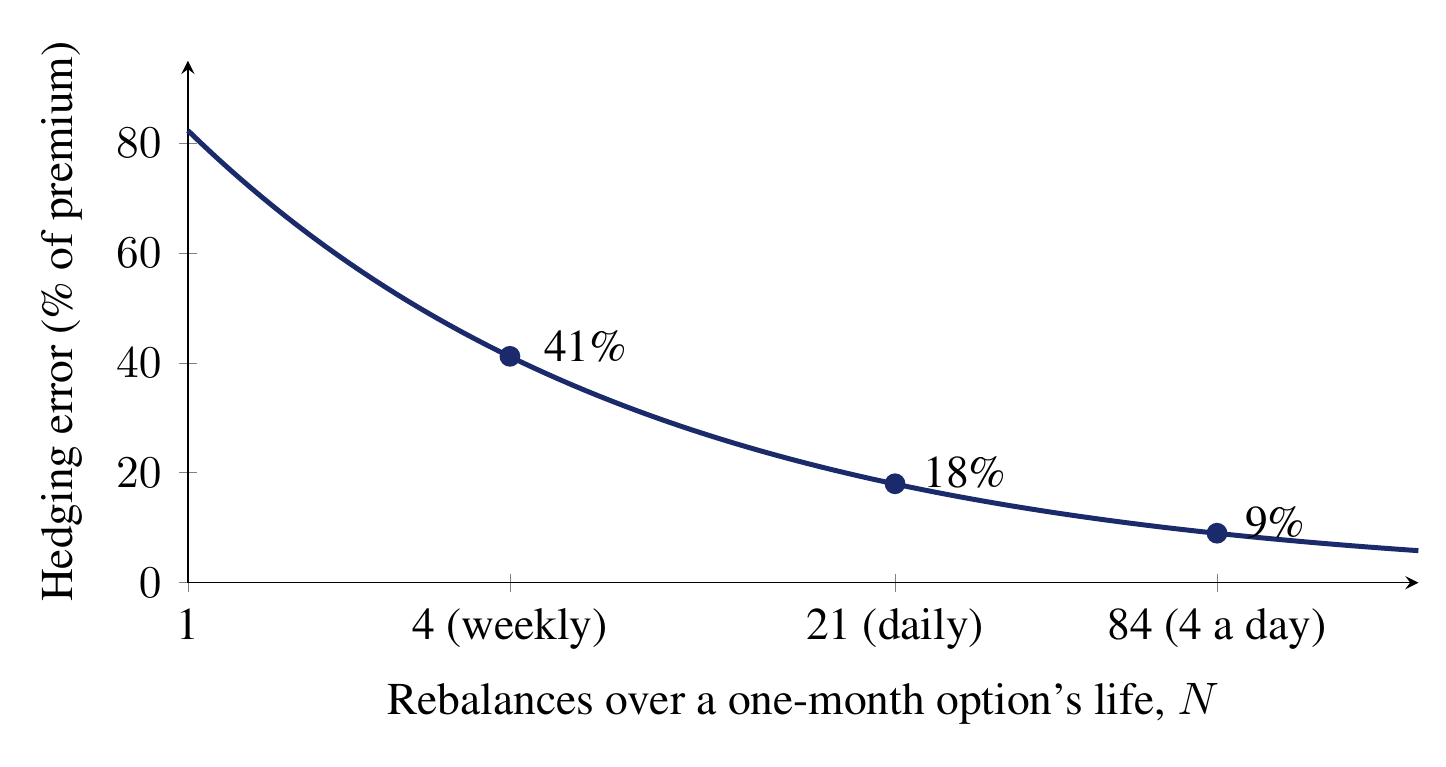
\includegraphics[width=0.85\linewidth]{images/fig15-1-hedge-frequency.png}
\caption{Hedging error in the Black--Scholes world, by the Kamal--Derman approximation, for a one-month at-the-money option at 20\% volatility. Hedging weekly leaves an error of about 41\% of the premium, daily about 18\%, and four times a day about 9\%. Each quadrupling of the frequency halves the error.}
\label{fig:15-freq}
\end{figure}

\textbf{The volatility smile.} If Black--Scholes were right, every option on the same asset would have the same implied volatility. In practice, implied volatility varies with the strike: for stock indexes, low-strike puts trade at much higher implied volatilities than at-the-money options. This \textbf{skew} or \textbf{smile} is the market's admission that returns are not lognormal with constant volatility.

\textbf{Worked example.} The index is at 100, the risk-free rate is 4\%, and a one-month at-the-money call is sold at 20\% implied volatility (Figure~\ref{fig:15-pnl}).

\begin{itemize}
  \item Price \$2.47, delta 0.53, gamma 0.069, theta $-\$0.063$ a day. The dealer sells the call and buys 0.53 units of the index.
  \item If the index is unchanged the next day, the dealer earns the theta: about \$0.063.
  \item If the index moves 3 points either way, the gamma loss is $\tfrac{1}{2} \times 0.069 \times 3^2 = \$0.31$, and the dealer loses about $\$0.31 - \$0.063 = \$0.25$ before rebalancing.
  \item The break-even daily move is $\sqrt{2 \times 0.063/0.069} \approx 1.35$ points, close to the 1.26-point daily standard deviation that 20\% annual volatility implies. Hedging is a wager that daily moves will average less than that.
\end{itemize}

\begin{figure}[htbp]
\centering
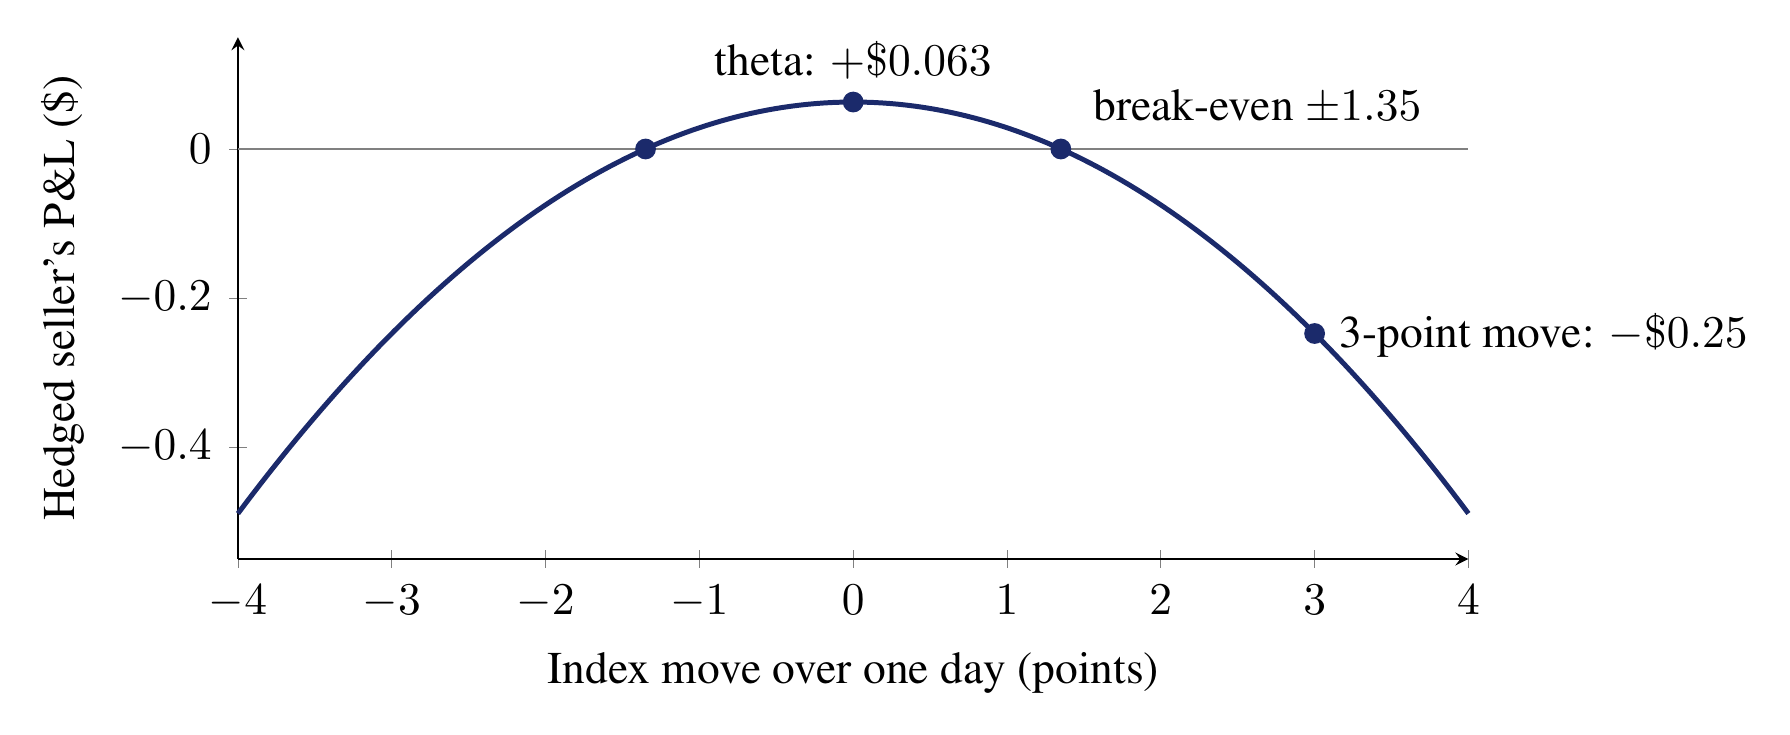
\includegraphics[width=0.85\linewidth]{images/fig15-2-hedge-pnl.png}
\caption{The delta-hedged call seller's P\&L over one day in the worked example. The seller earns \$0.063 of theta if the index is unchanged, breaks even on a move of about 1.35 points either way, and loses \$0.25 on a 3-point move. The loss grows with the square of the move.}
\label{fig:15-pnl}
\end{figure}

\textbf{Further reading.} Hull, \emph{Options, Futures, and Other Derivatives} (the Black--Scholes--Merton model, the Greeks, delta hedging, volatility smiles); Wilmott, \emph{Paul Wilmott Introduces Quantitative Finance} (hedging and the hedging P\&L); Shreve, \emph{Stochastic Calculus for Finance II} (replication); Gatheral, \emph{The Volatility Surface}.

\section{How it works}
\label{sec:15-how}

The replication argument can fail in four ways, and each leaves a different fingerprint on the hedging P\&L.

\begin{center}
\small
\begin{tabularx}{0.9\linewidth}{@{}>{\raggedright\arraybackslash}p{0.2\linewidth}>{\raggedright\arraybackslash}X>{\raggedright\arraybackslash}X@{}}
\toprule
Assumption & What happens in practice & Effect on a hedged option seller \\
\midrule
Continuous trading & Hedgers rebalance daily or less often & Random errors that shrink with hedging frequency; present even when the model is right \\
Constant, known volatility & Volatility changes and clusters (Chapter 11) & P\&L tracks realized minus implied variance; losses when volatility rises \\
Continuous price paths & Prices jump, as in October 1987 or March 2020 & Large losses on jump days that no rebalancing frequency can prevent \\
No trading costs & Every rebalance pays a spread & A steady drag that grows with hedging frequency \\
\bottomrule
\end{tabularx}
\end{center}

The first is a property of the model itself: it would occur even if Black--Scholes were exactly right. The others are failures of its assumptions. A test of the claim must separate them, and the cleanest way is to run the same hedging strategy twice, once on real market paths and once on simulated paths that obey the model exactly. The difference between the two is the cost of the model's being wrong.

\textbf{Jumps are the hardest problem.} Over a day in which the market falls 20\%, the change in the option's value is far from the delta-hedge's change. The gamma term $\tfrac{1}{2}\Gamma\,dS^2$ is enormous, and rebalancing more often does not help, because the jump happens between rebalances. A seller of options is short gamma, so a jump in either direction is a loss.

\textbf{Volatility changes} are a second-order version of the same problem. If realized volatility over the month is twice the implied volatility used to price and hedge the option, the seller loses roughly vega times the gap, regardless of how often the hedge is adjusted.

\textbf{The smile is the market's response.} After October 1987, dealers began to charge more for the risks that delta hedging cannot remove: crashes and volatility spikes. They did so by raising the implied volatility of out-of-the-money puts, the options that pay off in crashes. The smile is thus both evidence against the Black--Scholes assumptions and the price of the residual risk that delta hedging leaves.

\section{The claim}
\label{sec:15-claim}

\begin{callout}
\textbf{Claim.} An option seller who delta-hedges as Black--Scholes prescribes is left with little risk. Hedging removes most of the variance of the unhedged position, and what remains is small, symmetric and shrinks as hedging becomes more frequent.
\end{callout}

This is the claim that justifies treating an option's Black--Scholes price as its cost of production. To test it we need to be precise on four points.

\begin{itemize}
  \item \textbf{Little risk relative to what.} The benchmark is the unhedged short option. A hedge that removes 90\% of its variance and leaves errors of a fifth of the premium, as in the Black--Scholes world with daily hedging, meets the claim. A hedge that leaves occasional losses of several times the premium does not.
  \item \textbf{Which volatility.} The seller must price and hedge at some volatility. We use the VIX, the market's implied volatility, so the test is whether hedging at the market's price leaves little risk.
  \item \textbf{Which statistic.} The standard deviation of the hedging error captures day-to-day risk. The 1\% quantile and the worst month capture tail risk. The claim requires both to be small.
  \item \textbf{What would count against it.} The claim fails if hedging on real paths leaves much more risk than on Black--Scholes paths, if the remaining errors are fat-tailed, or if more frequent hedging fails to reduce them.
\end{itemize}

\section{The original evidence}
\label{sec:15-evidence}

\textbf{The model.} Black and Scholes (1973) derived the option price from a hedging argument, and Merton (1973) generalized it and set out the conditions under which it holds. Early empirical tests, including their own (Black and Scholes 1972), found the model a useful approximation with systematic deviations from market prices. Within a few years Black--Scholes prices and deltas were standard on trading floors.

\textbf{Transaction costs.} Leland (1985) showed that with proportional trading costs, perfect replication is impossible: hedging continuously would cost an infinite amount. He proposed hedging at discrete intervals with an adjusted volatility, raised for an option seller to cover the expected costs, and showed that the adjustment grows as the hedging interval shrinks. Even in principle, the seller faces a trade-off between hedging error and trading costs.

\textbf{The smile after 1987.} Rubinstein (1994) documented that before October 1987, implied volatilities of S\&P 500 index options were roughly the same across strikes, as Black--Scholes requires. After the crash, a pronounced skew appeared, with low-strike puts priced at much higher implied volatilities, and it has persisted ever since. He developed implied binomial trees to fit it. The smile is direct evidence that the market does not price options as if Black--Scholes held.

\textbf{Better models.} Bakshi, Cao and Chen (1997) tested models with stochastic volatility, jumps and stochastic interest rates on S\&P 500 options. Adding stochastic volatility and jumps improved pricing. For hedging, modelling stochastic volatility alone gave the best performance; jumps helped pricing but not hedging, because a jump cannot be hedged with the underlying asset at all.

\textbf{Portfolio insurance.} The most consequential test of dynamic replication was not an academic study. In the 1980s, portfolio insurance programmes used dynamic trading in index futures to replicate a protective put on large equity portfolios. The Brady Commission (Presidential Task Force on Market Mechanisms 1988) estimated that \$60 to \$90 billion of equity assets were under portfolio insurance when the market crashed in October 1987. The What Failed box in Section~\ref{sec:15-investors} tells what happened.

\section{Replication lab: hedging options along real paths}
\label{sec:15-lab}

\begin{callout}
\textbf{Lab 15 at a glance.} \emph{Claim on trial:} delta hedging removes option risk. \emph{Data:} daily market returns from the Kenneth French library and the VIX from FRED, from 1990; both are free. \emph{Code:} runs as a script (\texttt{python lab15.py}) or as a notebook with a prediction prompt before each step.
\end{callout}

At each month end the lab sells a one-month at-the-money call on the market at its Black--Scholes price, using the VIX as the implied volatility. It buys $\Delta$ units of the index, finances them at the risk-free rate, rebalances on a schedule, and pays the option's payoff at expiry. The final value is the \textbf{hedging P\&L}, expressed as a share of the premium. The same strategy is then run on 20 simulated geometric Brownian motion paths per month, using that month's implied volatility, where the Black--Scholes assumptions hold exactly.

\textbf{Part A, residual risk.} Mean, standard deviation, skewness, 1\% quantile and worst month of the hedged P\&L for daily, two-day, weekly, two-weekly and no hedging, on real and simulated paths, and the share of the unhedged risk removed (Figure 15.3).

\textbf{Part B, source.} A regression of the actual P\&L on the gamma--theta approximation of Equation~\eqref{eq:15-pnl} summed over the month (Figure 15.5), and on the gap between implied and realized variance.

\textbf{Part C, frictions.} Hedging frequency (Figure 15.6) and transaction costs of 0 to 10 basis points per unit of index traded (Figure 15.7).

\textbf{Part D, tail.} The worst months, with the market move, implied and realized volatility and the largest daily move, and the share of all losses that came from the worst 5\% of months (Figure 15.4).

Two design choices matter for interpretation. First, pricing at the VIX overstates at-the-money implied volatility, as Chapter 14 explained, so the \emph{mean} hedged P\&L includes the variance risk premium plus some overstatement. The \emph{spread} of the P\&L, which is what the claim is about, is little affected. Second, a delta-hedged call and a delta-hedged put with the same strike are the same position, so the lab uses calls only.

\textbf{What the simulated run shows.} On the simulated Black--Scholes paths, daily hedging leaves a mean P\&L near zero and a standard deviation of about 17\% of the premium, in line with the Kamal--Derman formula, and the error falls steadily as hedging becomes more frequent. On the simulated GARCH paths with fat tails, which play the role of real paths in the test run, daily hedging still removes most of the unhedged risk. But the residual is larger, negatively skewed and concentrated: the worst 5\% of months produced most of the losses. The gamma--theta approximation explains most of the P\&L, and the largest deviations from it come in months with big daily moves. These results confirm that the code works. They say nothing about real markets. Run the lab on the real data to reach your own verdict.

\section{Stress tests}
\label{sec:15-stress}

\textbf{Hedging frequency.} In the Black--Scholes world, hedging four times as often halves the error (Figure~\ref{fig:15-freq}). On real paths, the part of the error that comes from discrete rebalancing falls in the same way, but the parts that come from jumps and volatility changes do not. If the lab finds that moving from weekly to daily hedging reduces risk much less on real paths than on simulated ones, the residual is dominated by risks that rebalancing cannot remove.

\textbf{Transaction costs.} Every rebalance pays a spread. With costs of a few basis points per unit of index traded, daily hedging can consume a large share of the seller's margin, which is why dealers hedge less often than the model prescribes and why Leland's adjusted volatility exists. The lab's cost experiment shows how quickly the trade-off bites.

\textbf{Crash months.} The months that matter are those with jumps: October 1987 (before the lab's sample), August 1998, October 2008, August 2011, August 2015, February 2018 and March 2020. In each, a one-month option sold at the start of the month at the prevailing implied volatility faced daily moves far larger than that volatility implied. Expect the hedged seller's worst months to be these, with losses of a multiple of the premium even with daily hedging.

\textbf{Realized versus implied volatility.} The gamma--theta approximation says the hedged P\&L is a bet that realized variance will be below implied. When implied volatility is above realized, as it is in most months (Chapter 14), the hedged seller earns a profit. That profit is not evidence that hedging removed risk. It is the variance risk premium, earned by bearing the risk that remains. A hedge that leaves a positive mean and a fat left tail has turned an option position into a short-volatility position, not into a riskless one.

\textbf{Model risk in the hedge ratio.} Black--Scholes deltas assume volatility does not change when the price moves. For stock indexes, volatility tends to rise when prices fall (Chapter 11). Hull and White (2017) showed that adjusting the delta for this relation, a \textbf{minimum-variance delta}, reduces hedging errors for index options. The size of the improvement is itself a measure of how wrong the Black--Scholes hedge ratio is.

\section{Verdict}
\label{sec:15-verdict}

\begin{callout}
\textbf{Verdict: fails as a description of practice} (as of October 2026). Black--Scholes delta hedging removes most of the day-to-day risk of an option position, but what it leaves is not little and not symmetric. The residual is a bet on realized versus implied volatility, with fat-tailed losses in months with jumps and volatility spikes, and those losses cannot be eliminated by hedging more often.
\end{callout}

What survives:

\begin{itemize}
  \item \textbf{Delta hedging works as a first approximation.} It removes most of the variance of an unhedged option position. It is the reason dealers can sell options without betting on market direction, and the reason Black--Scholes remains the industry's common language, even as a quoting convention.
  \item \textbf{The hedging P\&L is understood.} The gamma--theta approximation explains most of it. A trader knows what bet the hedged book contains: short realized volatility, long implied.
\end{itemize}

What fails:

\begin{itemize}
  \item \textbf{The residual is large and fat-tailed.} On real paths, hedging leaves more risk than on Black--Scholes paths, and the worst months bring losses of a multiple of the premium.
  \item \textbf{More frequent hedging cannot fix it.} Jumps happen between rebalances. Volatility changes are not hedged by the underlying at all. Hedging more often raises costs without removing these risks.
  \item \textbf{The market knows.} The volatility smile that has existed since 1987 is the market's price for the risks delta hedging leaves. If the claim were true, the smile would not exist.
\end{itemize}

The verdict would move to \emph{weakens} if a simple extension, such as hedging with a minimum-variance delta or adding a small position in other options to hedge vega and gamma, removed most of the tail. That is how dealers actually hedge, and it is why they never rely on delta alone.

\section{What investors can use}
\label{sec:15-investors}

\textbf{The residual risks inside structured products.} A bank that sells a structured note with a capped equity return or a principal guarantee is short options, and it hedges them dynamically. The hedge removes most of the market risk, but the bank keeps the risks this chapter identifies: jumps, volatility changes and the cost of rebalancing. It charges for them, which is part of why such products are expensive. When an investor buys one, the fee includes the price of risks the bank cannot hedge away.

\textbf{Option-based funds.} A fund that sells options and delta-hedges them is not market-neutral in the sense that matters. It is short volatility: it earns steady returns in calm markets and loses heavily in jumps. Its track record will look smooth until a crash.

\textbf{Why the smile exists.} The higher implied volatility of out-of-the-money index puts is not a quirk. It is the price of crash risk, which delta hedging cannot remove. An investor buying downside protection pays it; an investor selling protection is paid it for bearing the jumps.

\textbf{Questions to ask a manager or a structured-product issuer:}

\begin{itemize}
  \item How are the option positions hedged: delta only, or also vega and gamma with other options?
  \item What happens to the hedge in a one-day move of 10\% or 20\%?
  \item How often is the hedge rebalanced, and what does rebalancing cost?
  \item What was the strategy's worst month, and was it in a crash?
\end{itemize}

\begin{callout}
\textbf{What Failed: portfolio insurance, October 1987.} Portfolio insurance, developed by Hayne Leland and Mark Rubinstein, replicated a protective put on an equity portfolio by dynamic trading: selling stock-index futures as the market fell and buying them back as it rose, exactly as delta hedging prescribes. By October 1987, according to the Brady Commission, \$60 to \$90 billion of equity assets were under portfolio insurance.

On October 19, 1987, the market fell more than 20\% in a day. The strategy required insurers to sell at every step down. According to the Brady Commission, portfolio insurers sold the equivalent of about \$4 billion of stock in index futures, more than 40\% of futures volume excluding locals' trades, and just under \$2 billion of stock directly on the New York Stock Exchange. Prices moved faster than the trades could be executed, so the hedge was always behind. Insurers could not trade at the prices their models assumed, so the protection they delivered fell short of the puts they were replicating, and the Brady Commission concluded that their mechanical selling added to the pressure on prices.

The failure was the replication assumption itself: continuous trading at continuous prices. A real put would have paid off regardless of how the market got there. A replicated put depended on trading through the fall, and the market did not allow it. The volatility skew that appeared after the crash has been the market's price for that lesson ever since.
\end{callout}

\section{Open questions}
\label{sec:15-open}

\begin{itemize}
  \item \textbf{How much of the hedging error is compensation for bearing jump risk?} If the mean hedged P\&L of option sellers is positive, is it just enough to pay for the jumps, or more?
  \item \textbf{How much better do practical hedges do?} Minimum-variance deltas, vega hedges with other options and stochastic-volatility models all reduce hedging error. How much of the tail do they remove on real paths?
  \item \textbf{Do short-dated options change the picture?} Options expiring within a day have enormous gamma near expiry. Does dealers' hedging of them amplify intraday moves?
  \item \textbf{Can machine-learning hedges beat Black--Scholes?} ``Deep hedging'' learns hedging rules directly from data with costs and constraints. Do its gains survive out of sample and in crashes?
\end{itemize}

\section*{Exercises}
\addcontentsline{toc}{section}{Exercises}

\subsection*{Conceptual (all readers)}

\begin{enumerate}
  \item For the worked example in Section~\ref{sec:15-foundations}, compute the hedged seller's P\&L over one day if the index moves 1, 2 and 4 points. At what daily move does the seller break even?
  \item Using the Kamal--Derman approximation, Equation~\eqref{eq:15-kd}, compute the standard deviation of the hedging error, as a share of the premium, for a one-month at-the-money option hedged daily, weekly and four times a day.
  \item Show that a delta-hedged call and a delta-hedged put with the same strike and expiry have the same hedged P\&L.
\end{enumerate}

\subsection*{Lab extensions (technical readers)}

\begin{enumerate}
  \setcounter{enumi}{3}
  \item Part A: compare the share of unhedged risk removed by daily hedging on real and Black--Scholes paths. Compare the 1\% quantiles. Which comparison is more informative about the claim?
  \item Part B: what share of the variance of the hedged P\&L does the gamma--theta approximation explain? Find the months with the largest residuals. What happened in them?
  \item Part C: at what transaction cost does weekly hedging give a higher mean P\&L than daily hedging? What is the effect on the 1\% quantile?
  \item Part D: compute the share of all hedging losses that came from the worst 5\% of months. Compare it with the Black--Scholes paths.
  \item Price the option at the VIX but hedge using trailing 21-day realized volatility. How does the P\&L distribution change?
  \item A structured-product salesperson says the bank's position is ``fully hedged.'' Using this chapter's evidence, explain what risks the bank still carries and how it charges for them.
\end{enumerate}

\section*{References}
\addcontentsline{toc}{section}{References}

\begin{itemize}
  \item Bakshi, G., Cao, C. and Chen, Z. (1997). Empirical Performance of Alternative Option Pricing Models. \emph{Journal of Finance} 52(5): 2003--2049.
  \item Black, F. and Scholes, M. (1972). The Valuation of Option Contracts and a Test of Market Efficiency. \emph{Journal of Finance} 27(2): 399--417.
  \item Black, F. and Scholes, M. (1973). The Pricing of Options and Corporate Liabilities. \emph{Journal of Political Economy} 81(3): 637--654.
  \item Hull, J. and White, A. (2017). Optimal Delta Hedging for Options. \emph{Journal of Banking \& Finance} 82: 180--190.
  \item Kamal, M. and Derman, E. (1999). When You Cannot Hedge Continuously: The Corrections to Black--Scholes. \emph{Risk} 12(1).
  \item Leland, H. E. (1985). Option Pricing and Replication with Transactions Costs. \emph{Journal of Finance} 40(5): 1283--1301.
  \item Merton, R. C. (1973). Theory of Rational Option Pricing. \emph{Bell Journal of Economics and Management Science} 4(1): 141--183.
  \item Presidential Task Force on Market Mechanisms (1988). \emph{Report of the Presidential Task Force on Market Mechanisms} (the Brady Report). Washington, DC: U.S. Government Printing Office.
  \item Rubinstein, M. (1994). Implied Binomial Trees. \emph{Journal of Finance} 49(3): 771--818.
\end{itemize}

\textbf{Data:} Kenneth R. French Data Library, Fama/French 3 Factors [Daily]. Chicago Board Options Exchange, CBOE Volatility Index: VIX [VIXCLS], retrieved from FRED, Federal Reserve Bank of St.\ Louis.

\clearpage
\addcontentsline{toc}{chapter}{PART III: From Models to Agentic AI Systems}
\newpage

\vspace*{\fill}


\Large
\noindent\textbf{PART III: From Models to Agentic AI Systems}
\normalsize
\vspace*{3cm}


Part III extends anomaly detection beyond standalone models and into agentic AI systems, where models, tools, reasoning, and workflows work together to support intelligent decision-making. You will learn how to transform individual analytical methods into interactive systems capable of autonomous reasoning and multi-step problem solving.

\vspace*{0.5cm}

Chapter \ref{ch16}: From Models to Agentic AI Design Patterns

Chapter \ref{ch17}: Building the Streamlit User Interface

Chapter \ref{ch18}: Building the Agentic Skills

Chapter \ref{ch19}: Building the Agentic Engine

Chapter \ref{ch20}: Building the Agentic Tools

Chapter \ref{ch21}: Testing and Evaluating the Agentic AI System

Chapter \ref{ch22}: Governance, Reliability, and Risk Management

\vspace*{\fill}


% Chapter 16 -- Claim: Forward Rates Predict Future Interest Rates
% Requires: amsmath, amssymb, booktabs, array, tabularx, graphicx, tcolorbox (breakable, skins), hyperref or url.
% Defines the callout box only if the preamble has not.
\providecolor{fenavy}{HTML}{1B2A6B}
\providecolor{feshade}{HTML}{F3F5FA}
\makeatletter
\@ifundefined{callout}{%
  \newtcolorbox{callout}{breakable, enhanced,
    colback=white, colframe=gray!70, boxrule=0.5pt, arc=1mm,
    borderline west={2.5pt}{0pt}{gray!70},
    left=8pt, right=8pt, top=4pt, bottom=4pt}%
}{}
\makeatother

\chapter{Claim: Forward Rates Predict Future Interest Rates}
\label{ch:16}

When the yield curve slopes steeply upward, commentators read it as a forecast: markets expect interest rates to rise. When it inverts, they read it as a forecast of cuts and recession. Central banks extract ``market-implied'' policy paths from forward rates, and traders quote them as the market's view.

That reading rests on the oldest theory of the term structure, the \textbf{expectations hypothesis}: long rates are averages of expected future short rates, so forward rates are unbiased forecasts of where short rates are going. If it holds, a long bond and a sequence of short bonds earn the same expected return, and there is nothing to gain from choosing maturities.

The hypothesis is also one of the most thoroughly tested claims in finance. This chapter opens Part V, on rates, credit and currencies, with that test. The answer matters for anyone who reads the yield curve, manages a bond portfolio or prices an interest-rate derivative.

By the end of the chapter you will be able to:

\begin{itemize}
  \item compute zero-coupon yields, forward rates, holding-period returns and excess returns from bond prices;
  \item use duration to estimate a bond's price sensitivity to its yield;
  \item state the expectations hypothesis and define the term premium;
  \item explain the Fama--Bliss, Campbell--Shiller and Cochrane--Piazzesi tests and why they ask the same question;
  \item summarize the evidence, including the small-sample and out-of-sample critiques;
  \item read a market-implied rate path as a forecast plus a premium, and judge a bond strategy built on carry and roll-down.
\end{itemize}

\section{Foundations: yields, forward rates and the term premium}
\label{sec:16-foundations}

\textbf{Zero-coupon yields.} A zero-coupon bond pays \$1 at maturity $n$ and nothing before. Its price $P(n)$ defines its yield $y(n)$. With continuous compounding, $P(n) = e^{-n\,y(n)}$, so the log price is
\begin{equation}
  p(n) = -n\,y(n)
  \label{eq:16-logprice}
\end{equation}
Coupon bonds are portfolios of zeros, so the \textbf{zero-coupon yield curve} (yield against maturity) summarizes all Treasury prices. The Federal Reserve publishes a fitted curve back to 1961 (G\"urkaynak, Sack and Wright 2007).

\textbf{Forward rates.} Buying an $n$-year zero and selling an $(n-1)$-year zero locks in today a rate of return for the year from $n-1$ to $n$. That rate is the \textbf{forward rate} (Figure~\ref{fig:16-forward}):
\begin{equation}
  f(n) = p(n-1) - p(n) = n\,y(n) - (n-1)\,y(n-1)
  \label{eq:16-forward}
\end{equation}
A rising yield curve means forward rates above current yields.

\begin{figure}[htbp]
\centering
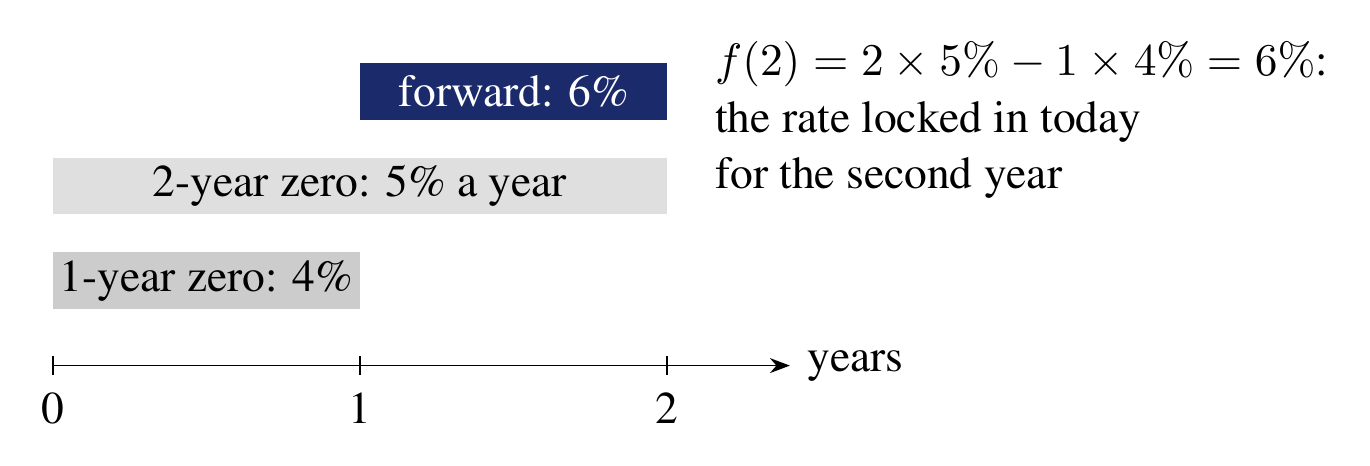
\includegraphics[width=0.85\linewidth]{images/fig16-1-forward.png}
\caption{A forward rate from the worked example. A two-year yield of 5\% is equivalent to earning the one-year yield of 4\% in the first year and a rate locked in today, the forward rate of 6\%, in the second.}
\label{fig:16-forward}
\end{figure}

\textbf{Holding-period returns.} Buying an $n$-year bond and selling it a year later, when it is an $(n-1)$-year bond, earns the log return
\begin{equation}
  r_{t+1}(n) = p_{t+1}(n-1) - p_t(n)
  \label{eq:16-hpr}
\end{equation}
The \textbf{excess return} $rx_{t+1}(n)$ subtracts the one-year yield $y_t(1)$, the return on a one-year bond held to maturity.

\textbf{Duration.} The percentage price change of a bond for a small change in its yield is approximately $-D \times \Delta y$, where $D$ is the \textbf{duration}. For a zero, $D$ equals its maturity. Long bonds are more sensitive to rates, which is why their returns are more volatile.

\textbf{The expectations hypothesis (EH)} states that the forward rate equals the expected future one-year rate, up to a constant:
\begin{equation}
  f_t(n) = E_t\!\left[y_{t+n-1}(1)\right] + \text{constant}
  \label{eq:16-eh}
\end{equation}
Equivalently, expected excess returns on bonds of all maturities are constant over time. The \textbf{term premium} is the gap between the forward rate and the expected future short rate, or between a long yield and the average expected short rate over its life. The EH says the term premium does not vary.

\textbf{Worked example.} The one-year zero yields 4\% and the two-year zero 5\% (continuously compounded).

\begin{itemize}
  \item Log prices: $p(1) = -0.04$, $p(2) = -0.10$. The one-year forward rate one year ahead is $f(2) = -0.04 + 0.10 = 6\%$.
  \item Under the EH, the market expects the one-year rate to be 6\% next year. If it is, the two-year bond, sold next year as a one-year bond, returns $-0.06 + 0.10 = 4\%$, the same as the one-year bond: excess return zero.
  \item If instead the one-year rate stays at 4\%, the two-year bond returns $-0.04 + 0.10 = 6\%$, an excess return of 2\%.
  \item A steep curve therefore forecasts either rising short rates (the EH) or high excess returns on long bonds (a term premium), or some mix (Figure~\ref{fig:16-readings}). The regressions in this chapter measure the mix.
\end{itemize}

\begin{figure}[htbp]
\centering
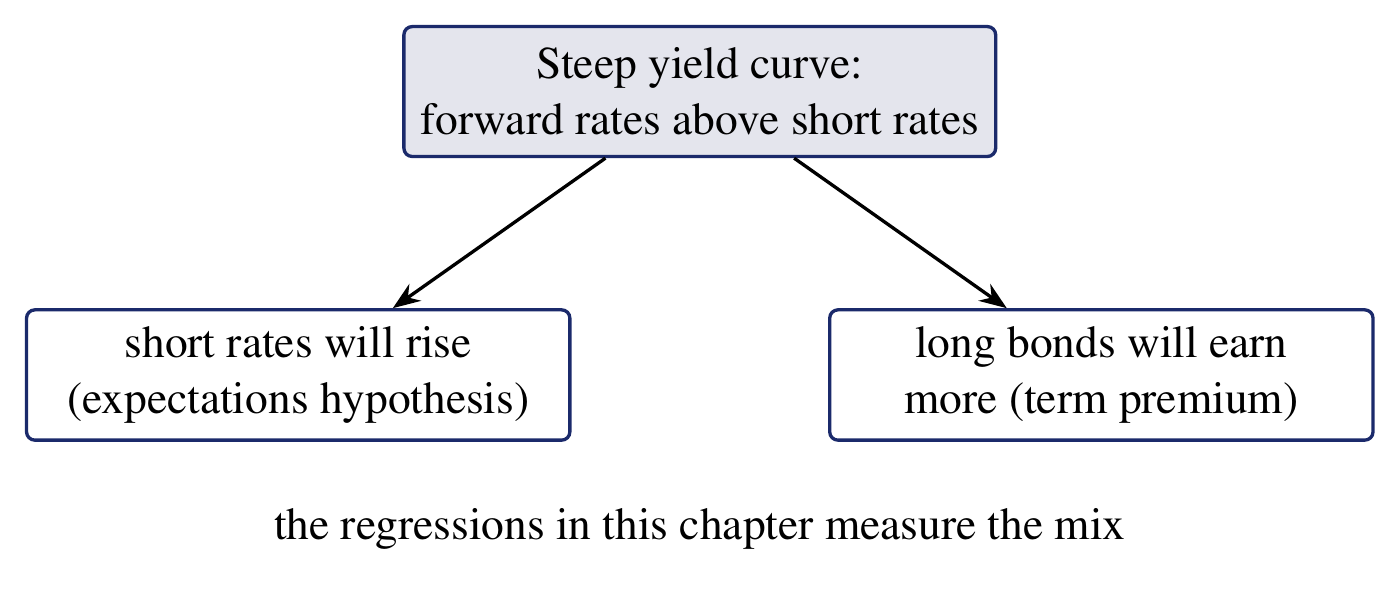
\includegraphics[width=0.75\linewidth]{images/fig16-2-two-readings.png}
\caption{Two readings of a steep yield curve. Forward rates above short rates can mean that short rates will rise, as the expectations hypothesis says, or that long bonds will earn more than short ones, a term premium. The tests in this chapter measure how much of each.}
\label{fig:16-readings}
\end{figure}

\textbf{Further reading.} Hull, \emph{Options, Futures, and Other Derivatives} (zero rates, forward rates, theories of the term structure); Fabozzi, \emph{Bond Markets, Analysis, and Strategies} (yield curve, duration); Cochrane, \emph{Asset Pricing} (term structure models and bond return predictability); Campbell, Lo and MacKinlay, \emph{The Econometrics of Financial Markets} (term structure of interest rates).

\section{How it works}
\label{sec:16-how}

The expectations hypothesis can be tested in three ways that look different but ask the same question.

\begin{center}
\small
\begin{tabularx}{0.9\linewidth}{@{}>{\raggedright\arraybackslash}p{0.17\linewidth}>{\raggedright\arraybackslash}X>{\raggedright\arraybackslash}p{0.15\linewidth}>{\raggedright\arraybackslash}X@{}}
\toprule
Test & Regression & Expectations hypothesis & Alternative: time-varying term premium \\
\midrule
Fama--Bliss, excess returns & $rx(n)$ on $f(n) - y(1)$ & Slope 0 & Slope positive (1 if forward spreads are all premium) \\
Fama--Bliss, short rates & $y(1)$ in $n-1$ years minus $y(1)$ today, on $f(n) - y(1)$ & Slope 1 & Slope below 1 \\
Campbell--Shiller & Change in the long yield over a year, on the scaled yield spread & Slope 1 & Slope below 1, even negative \\
\bottomrule
\end{tabularx}
\end{center}

The first two are mirror images. The forward spread equals the expected change in short rates plus the expected excess return, so a spread that does not forecast rising rates must forecast excess returns. The Campbell--Shiller test asks the question through long yields: if the curve is steep because short rates are expected to rise, long yields should rise too, as the bond approaches the higher short rates. If they fall instead, the steepness was a premium.

\textbf{Why the premium might vary.} Bonds lose value when inflation or rates rise unexpectedly. Investors demand compensation for that risk, and the compensation can change: higher in recessions, when investors are more risk-averse, and when inflation is uncertain. Supply and demand matter too. When pension funds and central banks buy long bonds, they push the term premium down. Any of these makes the EH fail.

\textbf{Why the tests are hard.} Interest rates are highly persistent, and annual returns sampled monthly overlap by eleven months. Both inflate $t$-statistics if handled carelessly (Chapter 3). The lab uses Newey--West errors with 18 lags and adds out-of-sample tests (Chapter 5).

\section{The claim}
\label{sec:16-claim}

\begin{callout}
\textbf{Claim (the expectations hypothesis).} Forward rates are unbiased forecasts of future short-term interest rates, up to a constant. A steep yield curve predicts rising short rates, not higher returns on long bonds.
\end{callout}

To test it we need to be precise on three points.

\begin{itemize}
  \item \textbf{Up to a constant.} The pure EH says forward rates equal expected short rates. Almost no one believes that, because long bonds have earned more than short ones on average. The testable version allows a constant term premium and denies only that it \emph{varies}.
  \item \textbf{Which horizon.} The tests use one-year holding periods, the standard in the literature. Fama and Bliss also examine longer horizons.
  \item \textbf{What would count against it.} The EH fails if forward spreads forecast excess bond returns (Fama--Bliss slope significantly above 0), if they forecast changes in short rates less than one for one, or if long yields fail to rise when the curve is steep (Campbell--Shiller slope significantly below 1). It fails convincingly if these patterns hold out of sample.
\end{itemize}

\section{The original evidence}
\label{sec:16-evidence}

\textbf{Fama and Bliss (1987).} Using discount bond prices constructed from CRSP Treasury data, Fama and Bliss found that the spread between the $n$-year forward rate and the one-year rate forecast one-year excess returns on $n$-year bonds, contradicting the EH. The same spread had little power to forecast changes in the one-year rate over the next year, but its power rose with the horizon: forward rates did contain information about short rates several years ahead, as interest rates mean-revert.

\textbf{Campbell and Shiller (1991).} Across maturities from a few months to ten years, the yield spread forecast long yields to move in the \emph{wrong} direction. When the curve was steep, long yields tended to fall over the following period, the opposite of what the EH requires, and the slope coefficients became more negative as maturity increased. A steep curve forecast high returns on long bonds, through rising prices.

\textbf{Cochrane and Piazzesi (2005).} Instead of one forward spread at a time, they regressed excess returns on all forward rates at once. A single factor, a tent-shaped combination of forward rates, forecast one-year excess returns on bonds of all maturities, with $R^2$ values up to 43\% in their sample. The factor was largely unrelated to the level, slope and curvature of the yield curve and rose in bad times, consistent with a risk premium that is high in recessions.

\textbf{The skeptics.} The evidence for the EH's failure is now widely accepted. The strength of the more ambitious claims is not. Bauer and Hamilton (2018) showed that standard tests suffer serious small-sample distortions with persistent predictors and overlapping returns. With more robust tests, the evidence that variables beyond level, slope and curvature forecast bond returns, including the Cochrane--Piazzesi factor, became much weaker. Thornton and Valente (2012) found that forecasts from forward rates gave little economic value out of sample to an investor choosing between bonds.

\section{Replication lab: the Treasury curve since 1961}
\label{sec:16-lab}

\begin{callout}
\textbf{Lab 16 at a glance.} \emph{Claim on trial:} forward rates are unbiased forecasts of future short rates. \emph{Data:} the Federal Reserve's zero-coupon Treasury yield curve (G\"urkaynak, Sack and Wright 2007), month-end yields for maturities of one to ten years; free and updated regularly. \emph{Code:} runs as a script (\texttt{python lab16.py}) or as a notebook with a prediction prompt before each step.
\end{callout}

\textbf{Part A, the classic tests.} Fama--Bliss regressions of one-year excess returns on forward spreads for maturities of 2 to 10 years, the companion regression of future short-rate changes on forward spreads, and Campbell--Shiller regressions for maturities of 2 to 10 years (Figures 16.4 and 16.5). Standard errors are Newey--West with 18 lags to account for the overlapping monthly observations.

\textbf{Part B, Cochrane--Piazzesi.} The average excess return on 2- to 5-year bonds regressed on the one-year yield and four forward rates; the loading of each maturity on the resulting factor; and out-of-sample forecasts from 1985 with an expanding window and an 11-month gap so that no training target overlaps the forecast date. Three predictor sets are compared with the historical mean: the full forward curve, a single forward spread and the level of rates alone (Figure 16.6).

\textbf{Part C, subperiods.} The Fama--Bliss slope for 5-year bonds, the Campbell--Shiller slope at the longest maturity and the Cochrane--Piazzesi $R^2$ in four periods: the start to 1984, 1985--2007, 2008--2015 (the zero lower bound) and 2016 onward.

\textbf{Part D, the investor's view.} Average excess returns by maturity, and returns after steep versus flat curves, with ``steep'' defined using only past information (Figure 16.7).

Two caveats apply. The Fed's curve is a fitted curve, not a set of traded bonds, and the classic studies used discount bonds constructed from CRSP data, which are not free. Results will be similar in spirit but not identical. Ten-year yields begin in 1971, so the longest maturities use a shorter sample.

\textbf{What the simulated run shows.} The simulation adds a time-varying term premium to the expected path of short rates, so the EH is false by construction. The lab finds what it should: Fama--Bliss slopes of about 0.6 to 0.7, significantly above zero; Campbell--Shiller slopes negative and well below 1; higher excess returns after steep curves. The tests on data where the EH holds exactly recover slopes of 0 and 1. These results confirm that the code works. They say nothing about real markets. Run the lab on the real data to reach your own verdict.

\section{Stress tests}
\label{sec:16-stress}

\textbf{Subperiods.} The postwar sample contains very different monetary regimes: the inflation of the 1970s, the Volcker disinflation, the long decline in rates from the 1980s, the zero lower bound after 2008 and the rapid tightening of 2022--23. A term premium that varies with inflation uncertainty would be most visible in the first half. Part C shows whether the rejection of the EH is a product of one era.

\textbf{The zero lower bound.} From 2008 to 2015 the short rate was pinned near zero. Forward rates still moved, driven by expectations of when the Fed would lift rates and by the term premium, but realized short rates did not. Regressions over this period behave differently, and the long-standing evidence may not carry over to it.

\textbf{Maturities.} The EH is a statement about all maturities. If it fails at two years but nearly holds at ten, or the reverse, that is informative about where the term premium lives.

\textbf{Out of sample.} In-sample $R^2$ values for bond return forecasts are inflated by persistent predictors and overlapping returns. The lab's out-of-sample test, which uses only data available at each date and leaves an 11-month gap, is the honest test. A negative out-of-sample $R^2$ would mean that an investor would have done better using the historical mean.

\textbf{Small samples.} Bauer and Hamilton (2018) showed that standard errors can understate uncertainty badly in these regressions. Their bootstrap tests are beyond this lab, but Exercise 4 asks how far the lab's $t$-statistics can be trusted. Treat $t$-statistics near 2 with suspicion.

\section{Verdict}
\label{sec:16-verdict}

\begin{callout}
\textbf{Verdict: fails} (as of October 2026). Forward rates are not unbiased forecasts of future short rates. Bond risk premia vary over time, and the slope of the yield curve forecasts excess returns on long bonds, not just changes in short rates. The more ambitious claim, that a richer function of the forward curve forecasts bond returns with high $R^2$, is weaker than it once appeared, but that does not rescue the expectations hypothesis.
\end{callout}

What fails:

\begin{itemize}
  \item \textbf{Forward spreads forecast excess returns.} In the classic studies and their updates, Fama--Bliss slopes are positive and significant. The forward spread is partly a forecast of rates and partly a premium for holding long bonds.
  \item \textbf{Long yields move the wrong way.} Campbell--Shiller slopes are below 1, and often negative, across maturities. On average, a steep curve has been followed by falling, not rising, long yields.
  \item \textbf{The premium is counter-cyclical.} Expected bond excess returns are higher in bad times, which the EH rules out.
\end{itemize}

What survives:

\begin{itemize}
  \item \textbf{Forward rates contain information about future short rates}, especially at horizons of several years, because rates mean-revert. They are biased forecasts, not useless ones.
  \item \textbf{The term premium is hard to forecast precisely.} Small-sample corrections and out-of-sample tests weaken the case for large, exploitable predictability (Bauer and Hamilton 2018; Thornton and Valente 2012). The evidence is strong that the premium varies, and weaker on how well anyone can track it in real time.
\end{itemize}

The verdict would move to \emph{weakens} if the rejection of the EH were confined to one monetary regime and disappeared in the others.

\section{What investors can use}
\label{sec:16-investors}

\textbf{Read forward rates as forecasts plus a premium.} A market-implied path for policy rates, extracted from forwards or futures, includes a term premium. It overstates expected rate rises when the premium is positive and understates them when the premium is negative. Estimated term premiums, such as those published by the Federal Reserve Bank of New York from the Adrian, Crump and Moench (2013) model, are one way to separate the two, though they are model estimates with wide uncertainty.

\textbf{Carry and roll-down.} A bond investor in a steep curve earns two things if rates do not change: the extra yield of the longer bond (\textbf{carry}) and the price gain as the bond rolls down to lower yields at shorter maturities (\textbf{roll-down}). The EH says these are expected to be offset by rising rates. The evidence says they are not fully offset on average. Carry and roll-down are thus a reasonable guide to expected excess returns, not a guaranteed one.

\textbf{Duration is a bet.} Extending maturity when the curve is steep has been rewarded on average, but with the volatility of long bonds. In 2022, when rates rose sharply, long Treasuries suffered some of their worst losses on record.

\textbf{Questions to ask a bond manager:}

\begin{itemize}
  \item How much of the portfolio's expected return comes from carry and roll-down, and what happens if rates rise by the forward rates?
  \item Does the strategy assume forward rates are forecasts of future rates, or does it allow for a term premium?
  \item How did the strategy perform when the curve was inverted, and in 2022?
\end{itemize}

\begin{callout}
\textbf{What Failed: reading the yield curve as a pure forecast of policy.} Between June 2004 and June 2006 the Federal Reserve raised its policy rate from 1\% to 5.25\%. Under the expectations hypothesis, long-term yields should have risen as the path of short rates moved up. Instead, long yields fell during the first year of the tightening and ended the period little higher than where they began. In February 2005, Chairman Alan Greenspan called the behaviour of long rates a ``conundrum'' (Greenspan 2005).

The conundrum was a puzzle only if long yields were pure forecasts of short rates. Term-premium models attributed much of the decline to a falling term premium, which various explanations linked to lower inflation uncertainty, foreign official purchases of Treasuries and demand from pension funds. Investors and policymakers who read the long end of the curve as the market's forecast of policy rates misread both the market and its signal. The same error recurs whenever a change in the term premium is taken for a change in expected policy.
\end{callout}

\section{Open questions}
\label{sec:16-open}

\begin{itemize}
  \item \textbf{Has central-bank bond buying changed the term premium?} Large-scale asset purchases after 2008 and in 2020 were designed to lower long yields by reducing the term premium. Did they change its behaviour or its predictability?
  \item \textbf{Is the Cochrane--Piazzesi factor real?} Robust small-sample tests weaken it. Does it survive in other countries and in data after 2003?
  \item \textbf{What drives the term premium?} Inflation uncertainty, risk aversion, supply and demand all play a part. Which dominates now?
  \item \textbf{Do macroeconomic variables add to the yield curve?} Several studies find that measures of real activity forecast bond returns beyond yields. Does that evidence survive the same robust tests?
\end{itemize}

\section*{Exercises}
\addcontentsline{toc}{section}{Exercises}

\subsection*{Conceptual (all readers)}

\begin{enumerate}
  \item The 1-, 2- and 3-year zero yields are 3\%, 3.5\% and 4\% (continuously compounded). Compute the forward rates $f(2)$ and $f(3)$. Under the expectations hypothesis, what one-year rates are expected one and two years from now?
  \item Using the yields in Exercise 1, compute the one-year excess return on the 3-year bond if the yield curve is unchanged a year from now. What would the excess return be if the expectations hypothesis held?
  \item Show that the Fama--Bliss slopes for excess returns and for short-rate changes add up to 1 when the horizon is one year ($n = 2$).
\end{enumerate}

\subsection*{Lab extensions (technical readers)}

\begin{enumerate}
  \setcounter{enumi}{3}
  \item Part A: at which maturities is the Fama--Bliss slope significantly above 0? Is any significantly different from 1? Given Bauer and Hamilton's (2018) warning about small-sample distortions, which of these conclusions would you still trust, and why?
  \item Part A: how does the Campbell--Shiller slope change with maturity? Explain in words what a negative slope means for a bond investor.
  \item Part B: compare the in-sample and out-of-sample $R^2$ of the Cochrane--Piazzesi regression. Which of the three predictor sets does best out of sample?
  \item Part C: in which subperiod is the evidence against the hypothesis strongest? What happened in 2008--2015?
  \item Part D: build a strategy that holds the 5-year bond after a steep curve and the 1-year bond otherwise. Compare its average excess return and Sharpe ratio with always holding the 5-year bond.
  \item A newspaper reports that ``markets expect three rate cuts next year,'' based on futures prices. Using this chapter's evidence, explain what the futures prices actually tell us.
\end{enumerate}

\section*{References}
\addcontentsline{toc}{section}{References}

\begin{itemize}
  \item Adrian, T., Crump, R. K. and Moench, E. (2013). Pricing the Term Structure with Linear Regressions. \emph{Journal of Financial Economics} 110(1): 110--138.
  \item Bauer, M. D. and Hamilton, J. D. (2018). Robust Bond Risk Premia. \emph{Review of Financial Studies} 31(2): 399--448.
  \item Campbell, J. Y. and Shiller, R. J. (1991). Yield Spreads and Interest Rate Movements: A Bird's Eye View. \emph{Review of Economic Studies} 58(3): 495--514.
  \item Cochrane, J. H. and Piazzesi, M. (2005). Bond Risk Premia. \emph{American Economic Review} 95(1): 138--160.
  \item Fama, E. F. and Bliss, R. R. (1987). The Information in Long-Maturity Forward Rates. \emph{American Economic Review} 77(4): 680--692.
  \item Greenspan, A. (2005). Federal Reserve Board's Semiannual Monetary Policy Report to the Congress. Testimony before the Committee on Banking, Housing, and Urban Affairs, U.S. Senate, February 16.
  \item G\"urkaynak, R. S., Sack, B. and Wright, J. H. (2007). The U.S. Treasury Yield Curve: 1961 to the Present. \emph{Journal of Monetary Economics} 54(8): 2291--2304.
  \item Thornton, D. L. and Valente, G. (2012). Out-of-Sample Predictions of Bond Excess Returns and Forward Rates: An Asset Allocation Perspective. \emph{Review of Financial Studies} 25(10): 3141--3168.
\end{itemize}

\textbf{Data:} Board of Governors of the Federal Reserve System, The U.S. Treasury Yield Curve: 1961 to the Present (\texttt{feds200628.csv}).

% Chapter 17 -- Claim: Credit Spreads Compensate Mainly for Expected Default Losses
% Requires: amsmath, amssymb, booktabs, array, tabularx, graphicx, tcolorbox (breakable, skins), hyperref or url.
% Defines the callout box only if the preamble has not.
\providecolor{fenavy}{HTML}{1B2A6B}
\providecolor{feshade}{HTML}{F3F5FA}
\makeatletter
\@ifundefined{callout}{%
  \newtcolorbox{callout}{breakable, enhanced,
    colback=white, colframe=gray!70, boxrule=0.5pt, arc=1mm,
    borderline west={2.5pt}{0pt}{gray!70},
    left=8pt, right=8pt, top=4pt, bottom=4pt}%
}{}
\makeatother

\chapter{Claim: Credit Spreads Compensate Mainly for Expected Default Losses}
\label{ch:17}

A corporate bond pays more than a Treasury bond of similar maturity. The obvious explanation is that companies can default and the U.S. government, for practical purposes, does not. Investors demand a higher yield to cover the losses they expect when some borrowers fail to pay. On this view, the credit spread is an actuarial charge: default probability times loss given default.

The view is intuitive, it is how many investors think about credit, and it is how credit ratings are designed, since ratings rank bonds by their expected default losses. It is also testable, because a century of default data tells us how often bonds of each rating have defaulted and how much investors recovered.

This chapter tests it. The answer bears on what credit investors are paid for, why spreads rise in recessions, and why highly rated structured securities proved so dangerous in 2007--08.

By the end of the chapter you will be able to:

\begin{itemize}
  \item define credit spreads, default probabilities, recovery rates and loss given default;
  \item compute the expected-loss spread and the default rate that would justify an observed spread;
  \item explain the Merton model, in which equity is a call option on the firm's assets;
  \item distinguish real-world from risk-neutral default probabilities, and explain why the timing of defaults matters for the spread;
  \item state the claim that spreads mainly reflect expected losses, and summarize the evidence on the credit spread puzzle and the excess bond premium;
  \item judge what a credit investor is paid for, and when reaching for yield is likely to disappoint.
\end{itemize}

\section{Foundations: spreads, default and recovery}
\label{sec:17-foundations}

\textbf{Credit spread.} The yield on a corporate bond minus the yield on a Treasury of similar maturity. Moody's publishes long-run yield series for seasoned \textbf{Aaa} and \textbf{Baa} bonds, the highest and lowest investment-grade ratings, back to 1919. The \textbf{Baa--Aaa spread} compares two corporate yields and avoids some of the differences between corporate and Treasury bonds.

\textbf{Default probability (PD)} is the chance that the issuer fails to pay in a given year. Rating agencies publish historical default rates by rating. Moody's reported average annual default rates of 0.27\% for Baa issuers and essentially zero for Aaa over 1920--2006, and about 1\% for Ba, the highest speculative grade (Moody's Investors Service 2007).

\textbf{Recovery rate ($R$)} is the fraction of face value investors recover after default, measured by the bond's price shortly after default. Moody's reported an average of 38\% for senior unsecured bonds over 1982--2006. \textbf{Loss given default} is $1 - R$.

\textbf{Expected-loss spread.} A risk-neutral investor, one who cares only about expected payoffs, demands just enough extra yield to cover expected losses. For a one-year horizon with continuous compounding:
\begin{equation}
  \text{spread} = -\ln\!\left[1 - \mathrm{PD}\,(1 - R)\right] \approx \mathrm{PD}\,(1 - R)
  \label{eq:17-el}
\end{equation}
Any spread above this is compensation for something else: risk, illiquidity or taxes.

\textbf{Why spreads can exceed expected losses.}

\begin{itemize}
  \item \textbf{Risk premium.} Defaults cluster in recessions, when investors' other wealth is also falling. Risk-averse investors demand compensation for losses that arrive at bad times.
  \item \textbf{Liquidity.} Corporate bonds trade less often and at wider bid--ask spreads than Treasuries.
  \item \textbf{Taxes.} In the United States, interest on corporate bonds is subject to state income tax; interest on Treasuries is not.
\end{itemize}

\textbf{The Merton model.} Merton (1974) treated a firm's equity as a call option on its assets, with the face value of debt as the strike (Figure~\ref{fig:17-merton}). Default occurs if asset value falls below the debt at maturity. The model links credit spreads to leverage and asset volatility, and its descendants, \textbf{structural models}, are the standard tool for asking whether spreads are consistent with default risk.

\begin{figure}[htbp]
\centering
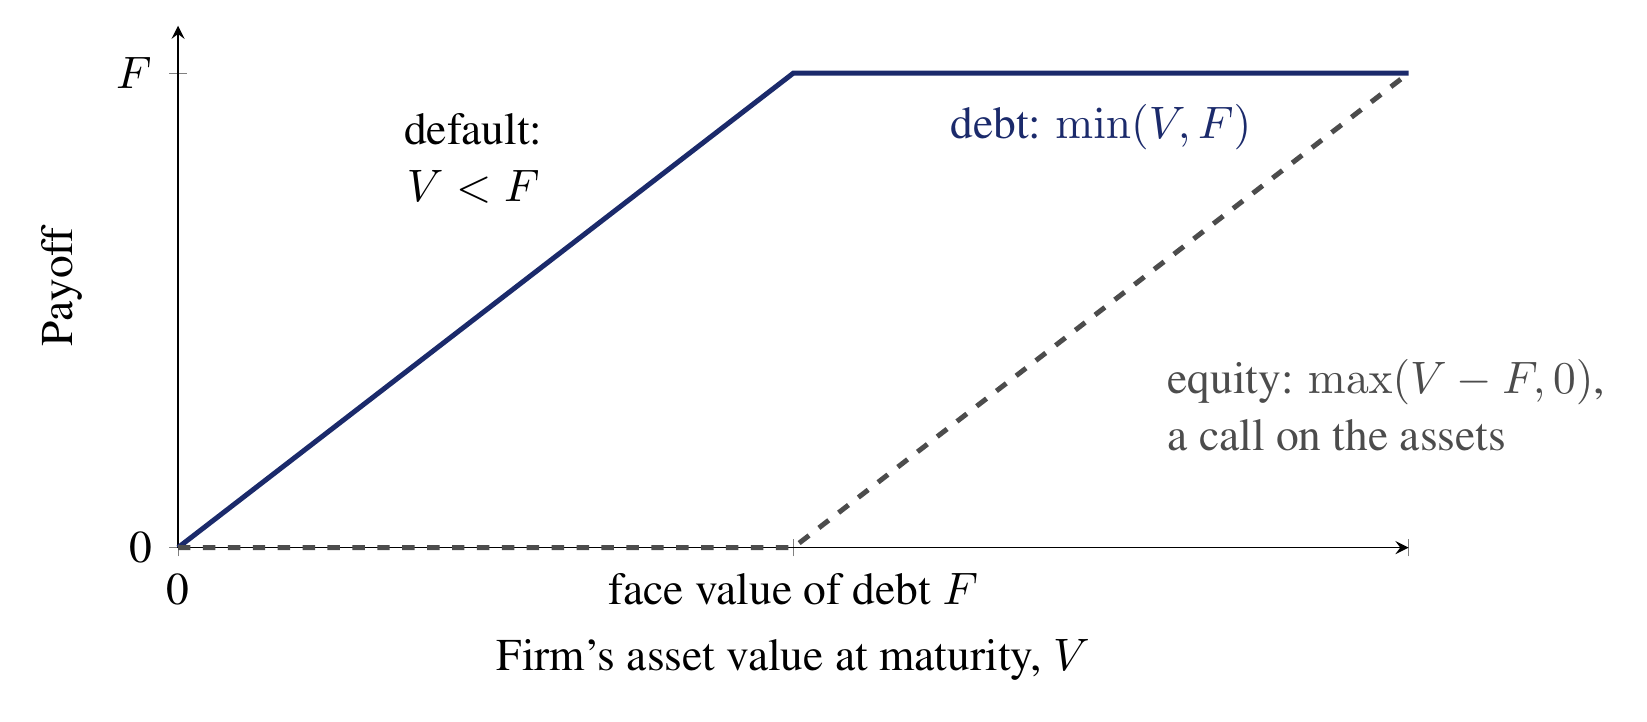
\includegraphics[width=0.85\linewidth]{images/fig17-1-merton.png}
\caption{The Merton model. At maturity, debtholders receive the firm's asset value $V$ up to the face value of debt $F$, so debt pays $\min(V, F)$. Shareholders receive what is left, $\max(V - F, 0)$, the payoff of a call option on the firm's assets. If $V < F$, the firm defaults.}
\label{fig:17-merton}
\end{figure}

\textbf{Worked example.} A 10-year Baa bond yields 6\% and a 10-year Treasury 4\%, a spread of 2\% (Figure~\ref{fig:17-decomp}).

\begin{itemize}
  \item With $\mathrm{PD} = 0.27\%$ and $R = 38\%$, the expected-loss spread is $-\ln(1 - 0.0027 \times 0.62) \approx 0.17\%$. Expected losses explain about 8\% of the spread.
  \item For expected losses to explain the whole 2\%, the annual default rate would have to be about $(1 - e^{-0.02})/0.62 \approx 3.2\%$, roughly twelve times the historical Baa average and well above the long-run average for Ba bonds.
  \item Even a pessimistic assumption, $\mathrm{PD} = 1\%$ and $R = 20\%$, explains only 0.8\% of the 2\% spread.
\end{itemize}

\begin{figure}[htbp]
\centering
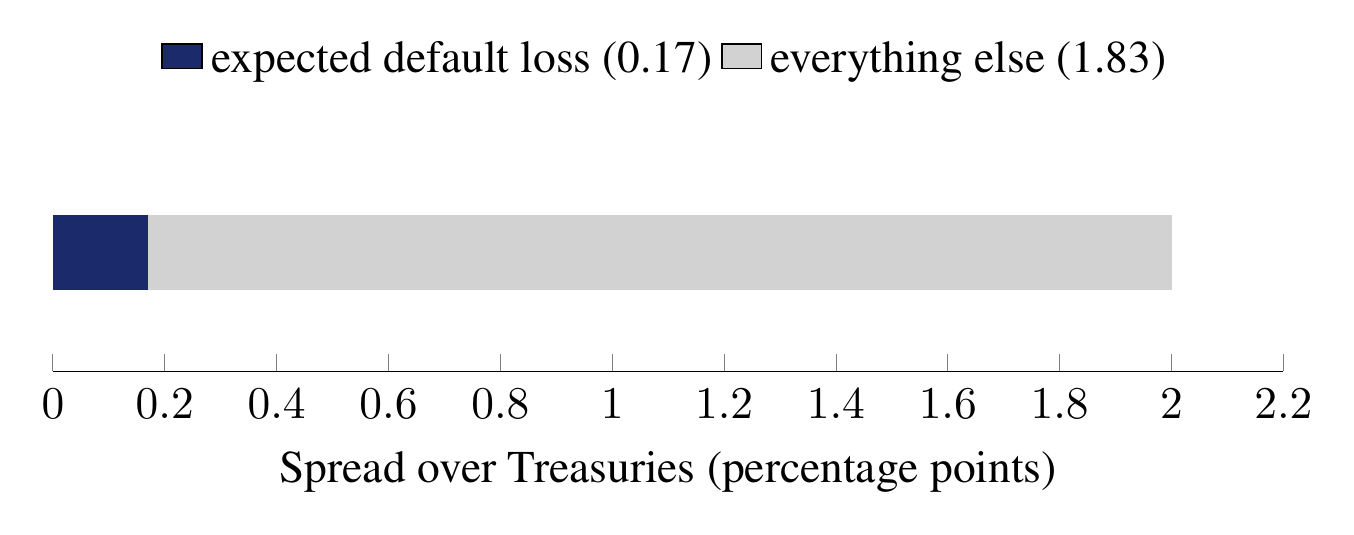
\includegraphics[width=0.85\linewidth]{images/fig17-2-spread-decomp.png}
\caption{Decomposing the worked example's 2\% Baa spread. At Moody's long-run default and recovery rates, expected default losses account for 0.17 percentage points. The remaining 1.83 points pay for something else: risk, illiquidity or taxes.}
\label{fig:17-decomp}
\end{figure}

\textbf{Further reading.} Hull, \emph{Options, Futures, and Other Derivatives} and \emph{Risk Management and Financial Institutions} (credit risk, default probabilities from bond prices, real-world versus risk-neutral probabilities, the Merton model); Fabozzi, \emph{Bond Markets, Analysis, and Strategies} (corporate bonds and credit spreads); Duffie and Singleton, \emph{Credit Risk: Pricing, Measurement, and Management}.

\section{How it works}
\label{sec:17-how}

A corporate bond's spread over a Treasury can be split into four pieces:

\begin{center}
\small
\begin{tabularx}{0.9\linewidth}{@{}>{\raggedright\arraybackslash}p{0.2\linewidth}>{\raggedright\arraybackslash}X>{\raggedright\arraybackslash}X@{}}
\toprule
Component & What it pays for & How to measure it \\
\midrule
Expected default loss & The average loss from defaults & Historical default rates $\times$ loss given default \\
Default risk premium & Bearing default losses that cluster in bad times & Residual after expected loss; structural models \\
Liquidity premium & Costs and delays of trading corporate bonds & Bid--ask spreads, trading volume, bond-specific measures \\
Tax premium & State taxes on corporate interest & Tax rates applied to the yield \\
\bottomrule
\end{tabularx}
\end{center}

The claim is that the first component dominates. The test has two steps. First, estimate expected losses from historical default and recovery data and compare them with observed spreads. If they explain most of the spread, the claim survives. Second, examine the residual. If it is small and stable, it might be liquidity or measurement error. If it is large, rises in recessions and forecasts economic activity, it behaves like a risk premium.

\textbf{Real-world and risk-neutral probabilities.} Bond prices imply a \textbf{risk-neutral} default probability: the default rate that would justify the spread for an investor who does not care about risk. Historical data give \textbf{real-world} default probabilities. The gap between the two measures how much investors charge for bearing default risk. Hull's textbooks show this gap is large for investment-grade bonds and smaller, relative to the spread, for junk bonds.

\textbf{Why the timing of defaults matters.} Two bonds with the same expected loss can deserve very different spreads. A bond whose defaults occur randomly over the cycle adds little risk to a diversified portfolio. A bond whose defaults all arrive in recessions, when stocks are falling and jobs are at risk, is much less attractive and should pay more. Investment-grade defaults are rare in normal times and concentrated in severe downturns, which is exactly the pattern that should command a large premium.

\section{The claim}
\label{sec:17-claim}

\begin{callout}
\textbf{Claim.} The yield spread of corporate bonds over Treasuries mostly reflects the losses investors expect from default. Under reasonable assumptions for default rates and recoveries, expected losses account for most of the average spread.
\end{callout}

To test it we need to be precise on three points.

\begin{itemize}
  \item \textbf{Mostly.} We take ``mostly'' to mean more than half of the average spread for investment-grade bonds. The claim could hold for junk bonds and fail for investment grade, or the reverse.
  \item \textbf{Reasonable assumptions.} Default and recovery rates vary over time and by measurement. The test uses long-run averages from rating agencies and checks how far they would have to be stretched to rescue the claim.
  \item \textbf{What would count against it.} The claim fails if expected losses explain less than half of investment-grade spreads under any plausible assumptions, and if the remainder behaves like compensation for risk: rising in recessions and forecasting weaker economic activity.
\end{itemize}

\section{The original evidence}
\label{sec:17-evidence}

\textbf{Elton, Gruber, Agrawal and Mann (2001).} Using corporate bond prices and historical default and recovery rates, they found that expected default losses accounted for only a small part of the spread between corporate and Treasury yields. State taxes, which apply to corporate interest but not to Treasury interest, explained a large part. The rest moved with the risk factors that explain stock returns, evidence of a risk premium.

\textbf{Collin-Dufresne, Goldstein and Martin (2001).} If spreads reflect default risk, changes in spreads should be explained by changes in the variables that drive default in structural models: leverage, asset volatility, interest rates. These explained only about a quarter of the variation in spread changes. Most of the rest was driven by a single common factor across bonds, unrelated to firm-specific default risk.

\textbf{Huang and Huang (2012).} They calibrated a wide range of structural models to historical default losses and equity risk premia and asked how much of observed spreads the models could explain. For investment-grade bonds, credit risk accounted for only a small share of spreads, and an even smaller share at short maturities. For high-yield bonds, it accounted for much more. This gap became known as the \textbf{credit spread puzzle}.

\textbf{Gilchrist and Zakraj\v{s}ek (2012).} They split corporate spreads into a component explained by expected default, estimated firm by firm, and a residual they called the \textbf{excess bond premium}. The excess bond premium, not the default component, carried most of the information about future economic activity. A rise in it predicted lower output and employment, consistent with a measure of investors' risk appetite and of the health of financial intermediaries.

Some later work narrows the puzzle by modelling default risk that varies with the business cycle. None restores expected losses as the main component of investment-grade spreads.

\section{Replication lab: a century of corporate spreads}
\label{sec:17-lab}

\begin{callout}
\textbf{Lab 17 at a glance.} \emph{Claim on trial:} credit spreads mainly reflect expected default losses. \emph{Data:} free monthly data from FRED: Moody's seasoned Aaa and Baa yields from 1919, the 10-year Treasury yield from 1953, the NBER recession indicator and industrial production. The Gilchrist--Zakraj\v{s}ek excess bond premium, published by the Federal Reserve, can be added. \emph{Code:} runs as a script (\texttt{python lab17.py}) or as a notebook with a prediction prompt before each step.
\end{callout}

\textbf{Part A, spreads.} The Baa--Aaa spread since 1919 and the Baa--Treasury and Aaa--Treasury spreads since 1953: averages, decade averages, and averages in recessions and expansions (Figure 17.3).

\textbf{Part B, decomposition.} The expected-loss spread from adjustable assumptions, by default 0.27\% a year for Baa and zero for Aaa with 38\% recovery, Moody's long-run averages. The lab reports the share of each average spread that expected loss explains, and the default rate that would be needed for expected loss to explain the whole spread at each date (Figures 17.4 and 17.5).

\textbf{Part C, the residual as a risk premium.} Regressions of industrial production growth over the next 12 months on each spread, and on the excess bond premium if supplied; growth by spread quintile; and the average path of the Baa--Aaa spread around the start of recessions (Figure 17.6).

\textbf{Part D, stress tests.} The share of the Baa--Treasury spread explained over a grid of default rates from 0.1\% to 2\% and recoveries from 20\% to 60\% (Figure 17.7), spread peaks in six crises, and subperiod averages.

Three measurement issues affect the decomposition, and they work in different directions.

\begin{itemize}
  \item \textbf{Maturity.} Moody's yields are on long bonds, typically 20 years or more, while the Treasury benchmark is 10 years. When the Treasury curve slopes up, this widens the Baa--Treasury spread for reasons unrelated to credit. The Baa--Aaa spread avoids the problem.
  \item \textbf{Taxes.} State taxes on corporate interest widen corporate--Treasury spreads, but not the Baa--Aaa spread.
  \item \textbf{Default timing.} Annual average default rates understate losses in the worst decades, such as the 1930s. Part D's grid includes default rates several times the average.
\end{itemize}

\textbf{What the simulated run shows.} The simulation builds the Baa--Aaa spread from a fixed expected loss of 0.15\% plus a premium that jumps in recessions. The lab recovers it: expected loss explains about a quarter of the Baa--Aaa spread, the spread is higher in recessions, and a high spread forecasts weaker output growth. These results confirm that the code works. They say nothing about real markets. Run the lab on the real data to reach your own verdict.

\section{Stress tests}
\label{sec:17-stress}

\textbf{Default assumptions.} The obvious defence of the claim is that historical averages understate future defaults. Part D's grid shows how far the assumptions must be stretched. With the 1920--2006 Baa average of 0.27\%, expected loss is a small fraction of a spread of one to two percentage points. To explain most of it, Baa bonds would need to default at well over 1\% a year with low recoveries, every year, which is the long-run experience of speculative-grade Ba bonds, not investment-grade Baa.

\textbf{The Great Depression.} The 1930s are the worst case for investment-grade defaults in the Moody's data. A default rate several times the long-run Baa average in those years would raise the expected-loss share sharply for that decade. Even then, the claim must explain the spread in the many decades with almost no Baa defaults.

\textbf{Crises.} Spreads peak in crises: the early 1930s, 1974--75, 1980--82, 2008--09 and March 2020. If spreads were expected losses, the peaks would forecast correspondingly large defaults. In 2008--09 and 2020, investment-grade defaults rose but remained far below what the peak spreads would have required. Spreads widened mainly because investors demanded more to hold risk and because dealers and funds withdrew from the market.

\textbf{Rating categories.} For high-yield bonds, expected losses are a much larger share of the spread (Huang and Huang 2012). The claim may work for junk bonds and fail for investment grade. Moody's yield series cover only Aaa and Baa, so this lab cannot test it directly; Exercise 1 extends the decomposition using published default rates for lower ratings.

\textbf{Liquidity.} Part of the residual is compensation for illiquidity, and it rises in crises when trading dries up. Separating liquidity from risk is difficult because both rise together in bad times. The Gilchrist--Zakraj\v{s}ek excess bond premium, which strips out firm-level default risk, is a useful check: if it forecasts output as well as the raw spread, the forecasting power does not come from expected defaults.

\section{Verdict}
\label{sec:17-verdict}

\begin{callout}
\textbf{Verdict: fails} (as of October 2026) for investment-grade bonds. Under historical default and recovery rates, expected default losses explain only a minority of investment-grade spreads, and the remainder behaves like a risk premium that rises in bad times and forecasts weaker economic activity. For high-yield bonds the claim fits better, since expected losses are a much larger share of their spreads.
\end{callout}

What fails:

\begin{itemize}
  \item \textbf{Expected losses are too small.} With Moody's long-run Baa default rate of 0.27\% and 38\% recovery, expected loss is under 0.2 percentage points a year, a small fraction of typical Baa spreads. Rescuing the claim requires default rates several times higher, sustained over decades.
  \item \textbf{Spreads move for other reasons.} Changes in default-risk variables explain only a quarter of spread changes (Collin-Dufresne, Goldstein and Martin 2001), and a common factor drives much of the rest.
  \item \textbf{The residual is a risk premium.} It rises in recessions, peaks in crises and forecasts weaker output, which is how compensation for bearing risk in bad times should behave (Gilchrist and Zakraj\v{s}ek 2012).
\end{itemize}

What survives:

\begin{itemize}
  \item \textbf{Expected losses matter at the margin.} Lower-rated bonds have higher spreads, and expected losses rise with them. Ratings rank spreads correctly even though they do not explain their level.
  \item \textbf{The claim fits junk bonds better.} For speculative-grade debt, expected losses are a large share of the spread.
\end{itemize}

The verdict would move to \emph{weakens} if a measure of liquidity explained most of the residual and that liquidity premium did not vary with economic conditions. The evidence so far points the other way: the residual and liquidity both rise in bad times.

\section{What investors can use}
\label{sec:17-investors}

\textbf{Credit is compensation for recession risk.} An investor in investment-grade bonds earns a spread well above expected default losses. That is good news on average, but it is pay for a specific risk: losses and price declines that arrive together with stock-market losses and recessions. Credit is not a substitute for Treasuries in a portfolio meant to hedge equity risk.

\textbf{The limits of reaching for yield.} In low-rate periods, investors move into lower-rated or longer-maturity credit to earn more. The extra yield is real, but it is paid for bearing more of the same recession risk. A portfolio that has quietly accumulated credit exposure will behave like an equity portfolio in a downturn.

\textbf{Ratings measure expected loss, not timing.} A rating ranks bonds by how likely they are to default and how much investors will lose, on average. It says nothing about whether those losses will arrive in a recession, which is what determines the risk premium.

\textbf{Questions to ask a credit manager:}

\begin{itemize}
  \item What share of the portfolio's yield above Treasuries would be lost in a recession with default rates like those of 2009?
  \item How correlated are the portfolio's returns with stocks in bad months?
  \item How liquid are the holdings in a crisis, and what would it cost to sell them?
  \item For structured holdings, how do losses depend on correlations between the underlying loans?
\end{itemize}

\begin{callout}
\textbf{What Failed: highly rated structured credit before 2008.} By 2007, according to Fitch, roughly 60\% of all global structured products carried AAA ratings, compared with less than 1\% of corporate issues (Coval, Jurek and Stafford 2009). Pooling mortgages and other loans and slicing them into \textbf{tranches}, claims with different priority on the pool's losses, allowed issuers to create large quantities of senior securities whose expected default losses, as estimated by rating models, were as low as those of the safest corporate bonds. They were priced accordingly, with spreads similar to other AAA debt.

The mistake was the claim this chapter tests: that a spread need only compensate for expected losses. Senior tranches lose money only when many underlying loans default together, which happens in a severe recession. Their losses are therefore concentrated in exactly the worst states of the world, and they deserved much larger risk premiums than corporate bonds with the same expected loss. In 2007, Moody's downgraded 31\% of the asset-backed CDO tranches it rated, including 14\% of those initially rated AAA, and many more were downgraded in 2008. Investors who had treated rating-based expected losses as the whole story discovered that the timing of losses matters as much as their average.
\end{callout}

\section{Open questions}
\label{sec:17-open}

\begin{itemize}
  \item \textbf{How much of the residual is liquidity rather than risk?} Both rise in bad times. Better measures of bond-level liquidity, and the growth of bond ETFs, offer new ways to separate them.
  \item \textbf{Has the investor base changed spreads?} Insurance companies, bond funds and ETFs hold most corporate bonds. Do their constraints, such as capital rules tied to ratings or redemption pressure, create premiums unrelated to default?
  \item \textbf{What did central-bank purchases do?} In 2020 the Federal Reserve announced purchases of corporate bonds, and spreads fell sharply. How much of the premium is the price of intermediaries' balance-sheet capacity?
  \item \textbf{Do structural models need fixing or replacing?} Models with time-varying risk and macroeconomic default risk narrow the credit spread puzzle. Do they fit the cross-section of spreads by rating and maturity as well as the average?
\end{itemize}

\section*{Exercises}
\addcontentsline{toc}{section}{Exercises}

\subsection*{Conceptual (all readers)}

\begin{enumerate}
  \item Using Moody's long-run average annual default rates (Ba about 1.1\%, B about 3.5\%) and 38\% recovery, compute the expected-loss spread for Ba and B bonds. If typical spreads are 3\% and 5\%, what share is expected loss? Compare with the Baa result.
  \item A 5-year Baa bond yields 5.5\% and the 5-year Treasury 4\%. What annual default rate, with 40\% recovery, would make expected losses equal the spread? What does this say about the risk-neutral and real-world default probabilities?
  \item Explain in words why a bond whose defaults all occur in recessions should pay a higher spread than one with the same expected loss whose defaults occur at random times.
\end{enumerate}

\subsection*{Lab extensions (technical readers)}

\begin{enumerate}
  \setcounter{enumi}{3}
  \item Part B: with the default assumptions, what share of the Baa--Treasury and Baa--Aaa spreads does expected loss explain? Why might the two shares differ?
  \item Part B: plot the break-even default rate. In which months was it lowest? Was it ever below the historical Baa default rate?
  \item Part C: does the Baa--Aaa spread forecast industrial production growth? If you have the excess bond premium, does it forecast better?
  \item Part D: find the default and recovery assumptions under which expected loss explains 75\% of the average Baa--Treasury spread. Are they plausible for investment-grade bonds?
  \item Subtract an estimate of the state tax effect (for example, a 4\% tax rate applied to the corporate yield) and recompute the residual. How much does it shrink?
  \item A pension fund wants to raise its yield by moving from Treasuries to Baa corporate bonds. Using this chapter's evidence, explain what the fund will be paid for and when it is likely to regret the move.
\end{enumerate}

\section*{References}
\addcontentsline{toc}{section}{References}

\begin{itemize}
  \item Collin-Dufresne, P., Goldstein, R. S. and Martin, J. S. (2001). The Determinants of Credit Spread Changes. \emph{Journal of Finance} 56(6): 2177--2207.
  \item Coval, J., Jurek, J. and Stafford, E. (2009). The Economics of Structured Finance. \emph{Journal of Economic Perspectives} 23(1): 3--25.
  \item Elton, E. J., Gruber, M. J., Agrawal, D. and Mann, C. (2001). Explaining the Rate Spread on Corporate Bonds. \emph{Journal of Finance} 56(1): 247--277.
  \item Gilchrist, S. and Zakraj\v{s}ek, E. (2012). Credit Spreads and Business Cycle Fluctuations. \emph{American Economic Review} 102(4): 1692--1720.
  \item Huang, J.-Z. and Huang, M. (2012). How Much of the Corporate-Treasury Yield Spread Is Due to Credit Risk? \emph{Review of Asset Pricing Studies} 2(2): 153--202.
  \item Merton, R. C. (1974). On the Pricing of Corporate Debt: The Risk Structure of Interest Rates. \emph{Journal of Finance} 29(2): 449--470.
  \item Moody's Investors Service (2007). \emph{Corporate Default and Recovery Rates, 1920--2006}. New York: Moody's.
\end{itemize}

\textbf{Data:} FRED, Federal Reserve Bank of St.\ Louis: Moody's Seasoned Aaa Corporate Bond Yield [AAA], Moody's Seasoned Baa Corporate Bond Yield [BAA], 10-Year Treasury Constant Maturity Rate [GS10], NBER Recession Indicator [USREC], Industrial Production [INDPRO]. Optional: Federal Reserve Board, Gilchrist--Zakraj\v{s}ek excess bond premium.

% Chapter 18 -- Claim: High-Interest Currencies Depreciate Enough to Offset Their Yield
% Requires: amsmath, amssymb, booktabs, array, tabularx, graphicx, tcolorbox (breakable, skins), hyperref or url.
% Defines the callout box only if the preamble has not.
\providecolor{fenavy}{HTML}{1B2A6B}
\providecolor{feshade}{HTML}{F3F5FA}
\makeatletter
\@ifundefined{callout}{%
  \newtcolorbox{callout}{breakable, enhanced,
    colback=white, colframe=gray!70, boxrule=0.5pt, arc=1mm,
    borderline west={2.5pt}{0pt}{gray!70},
    left=8pt, right=8pt, top=4pt, bottom=4pt}%
}{}
\makeatother

\chapter{Claim: High-Interest Currencies Depreciate Enough to Offset Their Yield}
\label{ch:18}

In 2007 a Japanese household could borrow yen at less than 1\% and deposit Australian dollars at more than 6\%. Japanese retail investors, nicknamed ``Mrs.\ Watanabe,'' and hedge funds did this on a large scale. If exchange rates had stayed put, the trade would have earned the difference, year after year.

Textbook theory says it should not work. If investors are risk-neutral and rational, a currency that pays a higher interest rate must be expected to fall by just enough to offset its yield advantage. Otherwise everyone would borrow in yen and lend in Australian dollars until the opportunity disappeared. This is \textbf{uncovered interest parity}, and it underpins much of international macroeconomics.

This chapter tests it, and it turns out to be one of the most persistent puzzles in finance. The test also shows what the carry trade's returns look like and how they end.

By the end of the chapter you will be able to:

\begin{itemize}
  \item quote exchange rates and measure currency returns in logs;
  \item compute a forward exchange rate from covered interest parity, and explain why arbitrage enforces it;
  \item state uncovered interest parity and compute the profit or loss on a carry trade;
  \item run and interpret the Fama regression, and explain the forward premium puzzle;
  \item compare the risk-premium, crash-risk and slow-adjustment explanations, and the evidence for each;
  \item judge what a currency carry fund is paid for and how it loses money.
\end{itemize}

\section{Foundations: exchange rates, forwards and interest parity}
\label{sec:18-foundations}

\textbf{Exchange rates.} The \textbf{spot rate} $S$ is the price of one currency in terms of another. In this chapter $S$ is the number of U.S. dollars per unit of foreign currency, so a rise in $S$ means the foreign currency has \textbf{appreciated}. Changes are measured in logs: $\Delta s_{t+1} = \ln(S_{t+1}/S_t)$.

\textbf{Forward rates and covered interest parity (CIP).} A forward contract fixes today the exchange rate $F$ for a trade at a future date. An investor can earn the dollar interest rate $i$ either directly, or by converting dollars to foreign currency, earning the foreign rate $i^*$, and converting back at the forward rate. Arbitrage makes the two equal:
\begin{equation}
  \frac{F}{S} = \frac{1 + i}{1 + i^*}, \qquad \text{or in logs,} \qquad f - s \approx i - i^*
  \label{eq:18-cip}
\end{equation}
The forward rate is below the spot rate for a high-interest currency: the \textbf{forward discount} equals the interest differential. CIP held closely until 2008 and has shown small but persistent deviations since (Du, Tepper and Verdelhan 2018).

\textbf{Uncovered interest parity (UIP)} goes further. It says the \emph{expected} future spot rate equals the forward rate, so the high-interest currency is expected to depreciate by the interest differential:
\begin{equation}
  E_t[\Delta s_{t+1}] = i_t - i^*_t
  \label{eq:18-uip}
\end{equation}
UIP has no arbitrage behind it. Holding a foreign currency unhedged is risky, so UIP holds only if investors require no premium for that risk.

\textbf{The carry trade.} Borrow in a low-interest currency, convert and invest in a high-interest currency, and convert back later without hedging. Its excess return is the interest differential plus the change in the exchange rate:
\begin{equation}
  rx_{t+1} = (i^*_t - i_t) + \Delta s_{t+1}
  \label{eq:18-carry}
\end{equation}
Under UIP its expected value is zero. Equivalently, the carry trade is buying high-interest currencies forward at a discount and hoping they do not fall by as much as the discount.

\textbf{Worked example.} The U.S. one-year rate is 1\%, the Australian rate 5\%, and the spot rate is \$0.70 per Australian dollar (Figure~\ref{fig:18-carry}).

\begin{itemize}
  \item CIP: the one-year forward rate is $0.70 \times 1.01/1.05 \approx \$0.673$.
  \item UIP: the expected spot rate in a year is also \$0.673, a 3.8\% depreciation.
  \item Carry trade: borrow \$1 million at 1\%, buy A\$1.429 million, invest at 5\% to get A\$1.5 million.
  \begin{itemize}
    \item Spot unchanged at \$0.70: proceeds \$1.05 million, repay \$1.01 million, profit \$40,000.
    \item Spot falls to \$0.673, as UIP predicts: proceeds \$1.01 million, profit zero.
    \item Spot falls 10\% to \$0.63: proceeds \$945,000, loss \$65,000.
  \end{itemize}
\end{itemize}

\begin{figure}[htbp]
\centering
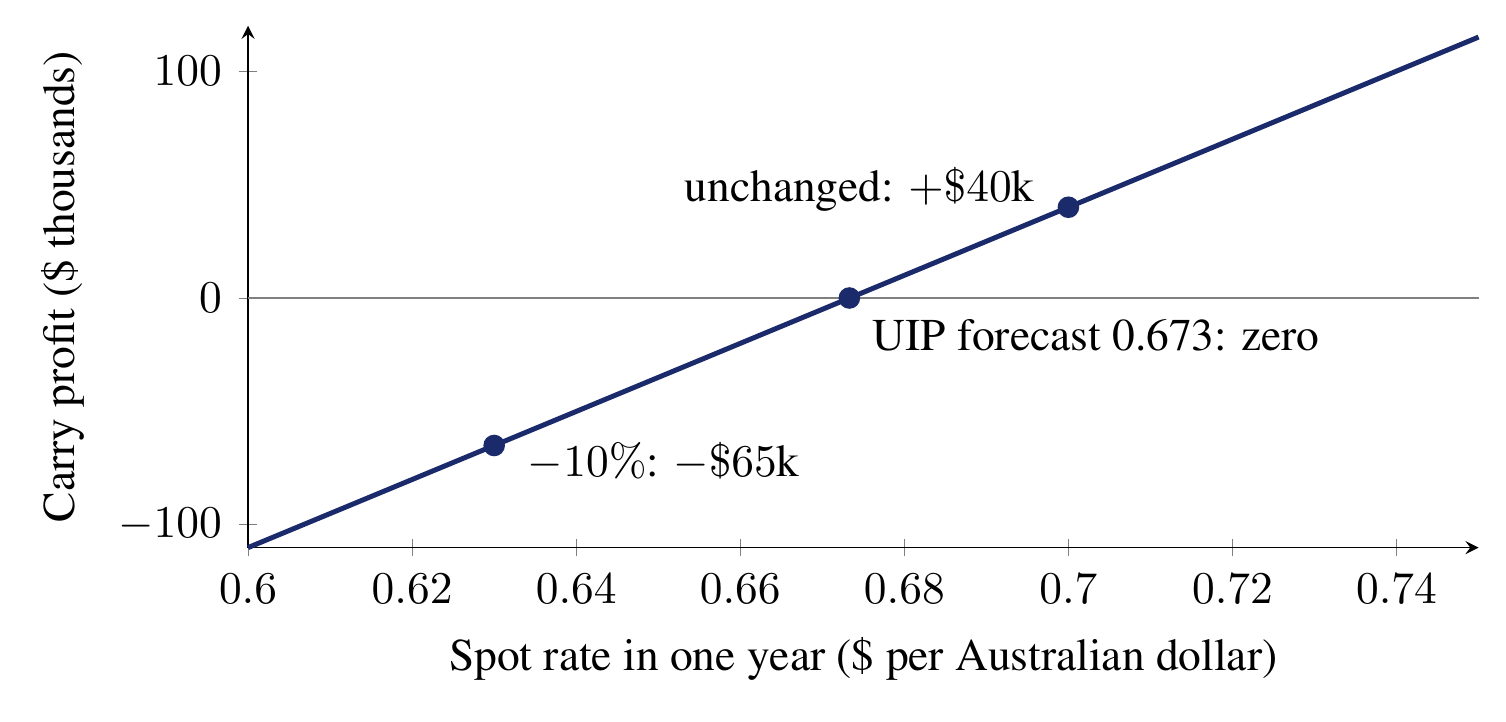
\includegraphics[width=0.85\linewidth]{images/fig18-1-carry-payoff.png}
\caption{Profit on the worked example's carry trade against the spot rate a year later. The trade earns \$40,000 if the Australian dollar is unchanged, breaks even at the UIP forecast of \$0.673, and loses \$65,000 if the currency falls 10\%.}
\label{fig:18-carry}
\end{figure}

\textbf{Further reading.} Hull, \emph{Options, Futures, and Other Derivatives} (foreign exchange forwards and futures, interest rate parity); Krugman, Obstfeld and Melitz, \emph{International Economics: Theory and Policy} (interest parity and exchange rate determination); Bodie, Kane and Marcus, \emph{Investments} (international diversification and currency risk); Cochrane, \emph{Asset Pricing} (the forward premium puzzle).

\section{How it works}
\label{sec:18-how}

UIP can be tested in two ways, one for each currency and one across currencies.

\textbf{The Fama regression.} Regress the change in the exchange rate on the lagged interest differential:
\begin{equation}
  \Delta s_{t+1} = a + b\,(i_t - i^*_t) + e_{t+1}
  \label{eq:18-fama}
\end{equation}
UIP implies $b = 1$: a one-point interest advantage for the foreign currency predicts a one-point depreciation. If $b = 0$, exchange rates are a random walk and the carry trade earns the whole differential. If $b < 0$, high-interest currencies tend to \emph{appreciate}, and the carry trade earns more than the differential (Figure~\ref{fig:18-fama}). This is the \textbf{forward premium puzzle}.

\begin{figure}[htbp]
\centering
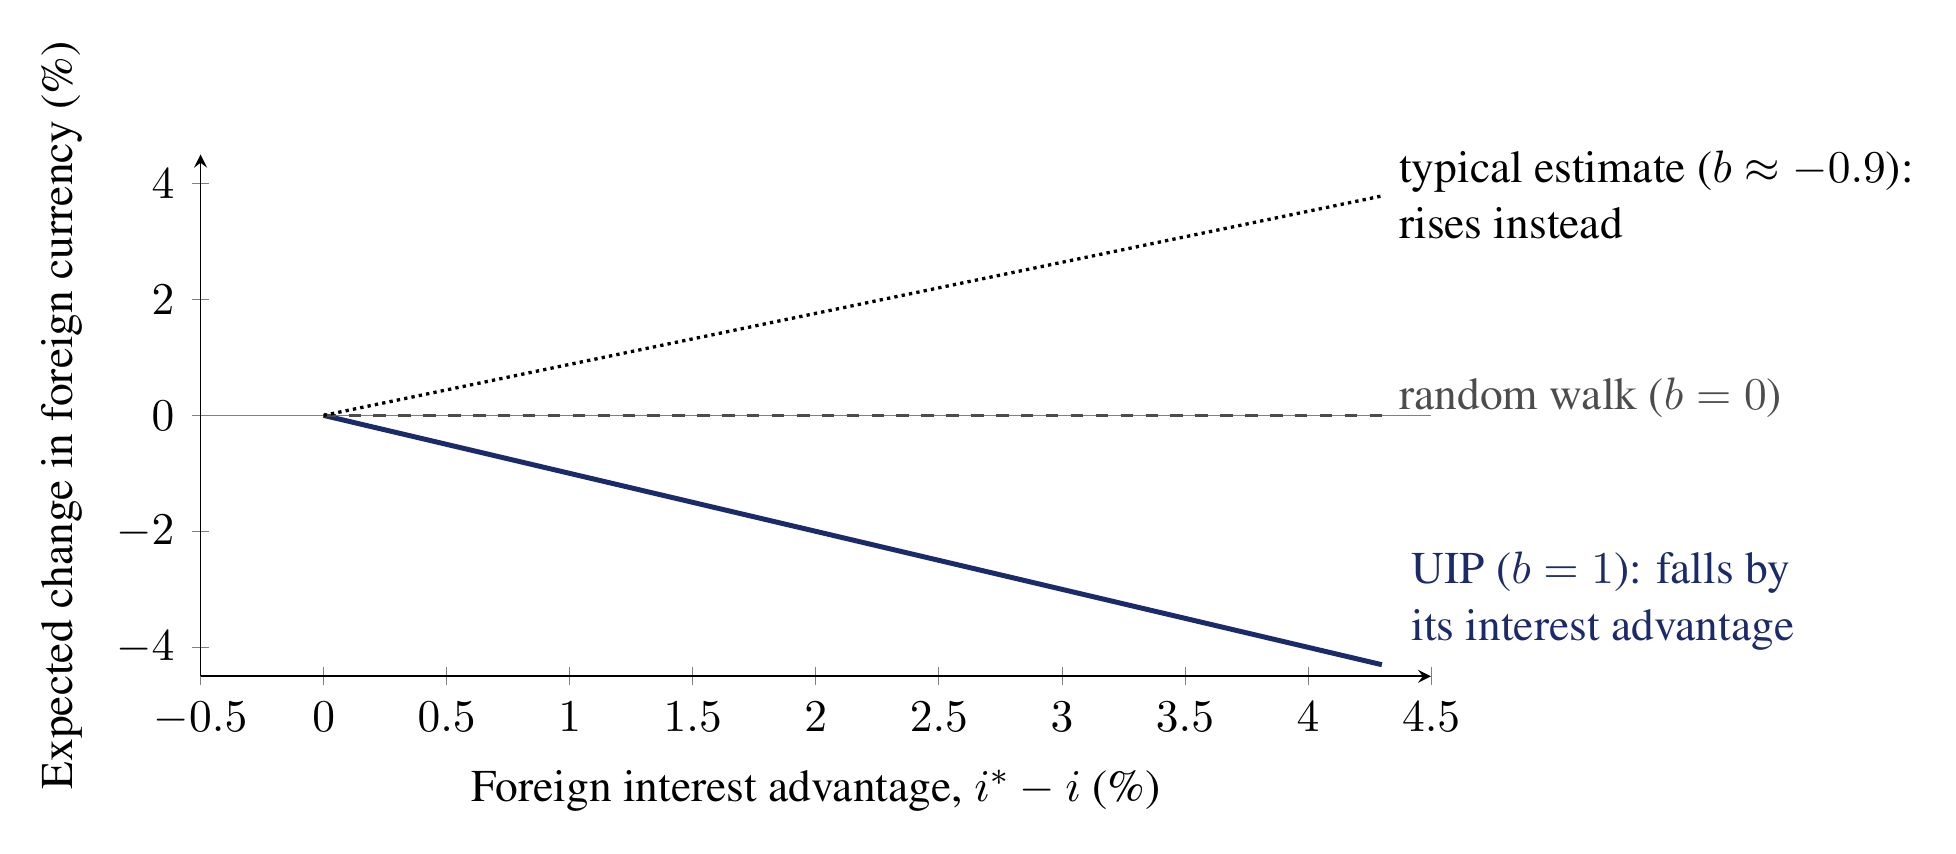
\includegraphics[width=0.85\linewidth]{images/fig18-2-fama-slope.png}
\caption{Three readings of the Fama regression. Under UIP ($b = 1$), a currency with a higher interest rate falls by its interest advantage. Under a random walk ($b = 0$), it is expected not to move. The typical estimate ($b \approx -0.9$, Froot and Thaler 1990) implies that it rises instead.}
\label{fig:18-fama}
\end{figure}

\textbf{Carry portfolios.} Each month, sort currencies by their interest rate, buy the highest-yielding ones and sell the lowest. If UIP holds, the portfolio earns nothing on average. Portfolios diversify away currency-specific noise and are what investors actually trade.

\textbf{Why UIP might fail.} There are three broad explanations.

\begin{itemize}
  \item \textbf{A risk premium.} High-interest currencies tend to fall in global downturns, when investors flee to the dollar, yen and Swiss franc. Investors demand a premium for holding them. Lustig, Roussanov and Verdelhan (2011) argue that carry returns compensate for exposure to a global risk factor.
  \item \textbf{Crash risk.} Carry returns may be steady most of the time and then collapse when carry traders all unwind at once, as funding dries up. The premium pays for those crashes (Brunnermeier, Nagel and Pedersen 2008).
  \item \textbf{Slow adjustment.} Investors may underreact to interest-rate changes, so currencies move toward UIP only gradually. That would be a mispricing rather than a risk premium, and should shrink as more capital pursues it.
\end{itemize}

These explanations make different predictions. A risk premium should show up as losses in bad times for the world economy. Crash risk should show up as negative skewness and losses concentrated in a few episodes. Slow adjustment should show up as a premium that declines over time and does not depend on market conditions.

\section{The claim}
\label{sec:18-claim}

\begin{callout}
\textbf{Claim (uncovered interest parity).} The currency of a high-interest country is expected to depreciate by its interest advantage, so borrowing in low-interest currencies and lending in high-interest ones earns nothing on average.
\end{callout}

To test it we need to be precise on three points.

\begin{itemize}
  \item \textbf{On average, over what period.} UIP is a statement about expectations. Over a few months, exchange-rate noise dominates. The test needs decades of data and many currencies.
  \item \textbf{Which currencies.} The lab uses nine developed-market currencies against the dollar. Emerging-market currencies have higher carry but also capital controls, default risk and much higher trading costs.
  \item \textbf{What would count against it.} UIP fails if Fama slopes are significantly below 1 and if a carry portfolio earns a significant average return. It fails in a deeper sense if the return survives trading costs and the slopes are below zero, not merely below one.
\end{itemize}

\section{The original evidence}
\label{sec:18-evidence}

\textbf{Fama (1984).} Using monthly data for nine currencies against the dollar after the end of fixed exchange rates in 1973, Fama found that the slopes were not just below 1 but generally negative. High-interest currencies tended to appreciate. He showed that this implies a risk premium in forward rates that varies over time and is more volatile than expected exchange-rate changes. Froot and Thaler (1990) summarized the literature: across 75 published estimates, the average slope was about $-0.88$.

\textbf{Carry as a risk factor.} Lustig, Roussanov and Verdelhan (2011) sorted currencies into portfolios by interest rate. The high-minus-low portfolio earned substantial average returns. They showed that a single carry factor, together with a dollar factor, explained much of the cross-section of currency returns, and that high-interest currencies loaded more heavily on it. Menkhoff, Sarno, Schmeling and Schrimpf (2012) found that carry losses coincided with increases in global currency volatility.

\textbf{Crashes.} Brunnermeier, Nagel and Pedersen (2008) showed that carry returns are negatively skewed: large losses are more likely than large gains. Losses coincided with falling risk appetite and funding liquidity, measured among other things by rises in the VIX, as carry traders were forced to unwind together.

\textbf{Peso problems.} One possible explanation is that the high returns compensate for rare disasters not yet seen in the sample, a \textbf{peso problem}. Burnside, Eichenbaum, Kleshchelski and Rebelo (2011) tested this by hedging carry positions with currency options. The hedged trade still earned a substantial return. They concluded that rare disasters could explain the premium only if the market prices them at much more than their likely cost.

\section{Replication lab: G10 currencies against the dollar}
\label{sec:18-lab}

\begin{callout}
\textbf{Lab 18 at a glance.} \emph{Claim on trial:} high-interest currencies depreciate enough to offset their yield. \emph{Data:} free monthly data from FRED: the Federal Reserve's exchange rates for nine currencies (yen, pound, Swiss franc, Canadian, Australian and New Zealand dollars, Swedish krona and Norwegian krone, and the euro from 1999) and OECD three-month interbank rates for each country and the United States. The VIX and the Fama--French market factor are optional. \emph{Code:} runs as a script (\texttt{python lab18.py}) or as a notebook with a prediction prompt before each step.
\end{callout}

\textbf{Part A, Fama regressions.} For each currency, the monthly change in the log exchange rate (dollars per foreign unit) on last month's U.S.-minus-foreign interest differential, with Newey--West errors, plus a pooled slope (Figure 18.3).

\textbf{Part B, the carry portfolio.} Each month, long the three highest-rate currencies and short the three lowest, equally weighted, using rates known at the end of the previous month. The return is split into the interest earned and the exchange-rate change (Figure 18.4). Its distribution is compared with a normal distribution (Figure 18.5).

\textbf{Part C, stress tests.} Three subperiods (to 1998, 1999--2007, 2008 onward), transaction costs of 0 to 20 basis points per unit of weight traded, exposure to stock-market returns and to changes in the VIX, and the ten worst months.

\textbf{Part D, the investor's view.} Drawdowns, recovery times, the share of losses from the worst months, and carry returns plotted against VIX changes (Figures 18.6 and 18.7).

Three data choices matter.

\begin{itemize}
  \item The interest differential stands in for the forward discount, which covered interest parity makes nearly equal; forward rates are not freely available.
  \item FRED's exchange rates are monthly averages of daily rates, which smooths returns and makes crashes look milder than they were.
  \item The sample is limited to developed currencies, where carry is smaller but trading costs and capital controls are minor.
\end{itemize}

\textbf{What the simulated run shows.} The simulation lets high-rate currencies depreciate by only 30\% of their interest advantage and adds rare risk-off months in which they fall sharply. The lab recovers this: a pooled Fama slope well below 1, a carry portfolio with a positive average return and negative skewness, interest income partly offset by exchange-rate losses, and losses when the VIX jumps. Individual currency slopes are very imprecise, as they are in real data. These results confirm that the code works. They say nothing about real markets. Run the lab on the real data to reach your own verdict.

\section{Stress tests}
\label{sec:18-stress}

\textbf{Subperiods.} Carry returns have varied a lot over time. A strategy that earns most of its return in a few long calm stretches and gives back much of it in a few months can look very different depending on where the sample starts and ends. The period since 2008 matters most: interest-rate differentials among developed countries collapsed toward zero for years, and with them the carry available.

\textbf{Transaction costs.} G10 currencies are the most liquid assets in the world, with bid--ask spreads of a few basis points. Carry portfolios rebalance only when interest rankings change, so turnover is modest. Costs reduce but rarely eliminate the developed-market carry premium. For emerging-market currencies they matter much more.

\textbf{Skewness and crashes.} The carry trade is often described as ``going up the stairs and down the elevator.'' Its returns should show negative skewness, and its worst months should cluster in episodes of global stress: 1992 (the European exchange-rate crisis), 1998 (the Russian default and LTCM), 2008, and the yen rally of August 2024. The lab lists the worst months and their share of total losses.

\textbf{Exposure to stocks and fear.} If carry is a risk premium, its returns should be positively correlated with stock returns, especially in bad months, and negatively correlated with changes in the VIX. A strategy whose beta to stocks rises in down markets offers less diversification than its average correlation suggests.

\textbf{Monthly averages.} Because the exchange rates are monthly averages of daily data, the lab's worst months will understate the speed of the real crashes. In October 2008 several carry currencies fell by double digits against the yen within days.

\section{Verdict}
\label{sec:18-verdict}

\begin{callout}
\textbf{Verdict: fails} (as of October 2026) over most samples. High-interest currencies have not depreciated by their interest advantage on average; Fama slopes are well below 1 and often negative, and carry portfolios have earned a premium. That premium is paid for with sudden crashes that arrive in global downturns.
\end{callout}

What fails:

\begin{itemize}
  \item \textbf{The slope.} Across decades of studies, slopes in the Fama regression have been below 1 and usually below zero. A high interest rate has predicted, if anything, a stronger currency in the short run.
  \item \textbf{The zero-return prediction.} Carry portfolios have earned positive average returns after realistic costs for developed-market currencies.
\end{itemize}

What survives:

\begin{itemize}
  \item \textbf{The spirit of UIP over long horizons and in extremes.} Some studies find slopes closer to 1 at horizons of several years, and in countries with very high inflation, where large interest differentials are matched by large depreciations.
  \item \textbf{No free lunch.} The premium comes with negative skewness, losses concentrated in global crises and positive correlation with stocks in bad months. That is what a risk premium looks like, not an arbitrage. An investor who earns carry is paid for providing liquidity and insurance to the rest of the world when it is scarce.
\end{itemize}

The verdict would move to \emph{weakens} if carry returns since 2008 were consistently near zero, as narrow interest differentials and crowding might imply.

\section{What investors can use}
\label{sec:18-investors}

\textbf{What a currency carry fund earns.} A carry strategy collects interest-rate differentials between currencies and keeps them as long as exchange rates do not move against it. In calm years it delivers modest, steady gains. Its risk is not spread evenly over time: most of its losses come in a few months of global stress, when high-yielding currencies fall together and funding currencies, the yen and Swiss franc above all, rise.

\textbf{How it loses money.} Carry crashes are fast. They begin when something forces leveraged carry traders to cut positions: a rise in volatility, a margin call, a surprise from the central bank of a funding currency. Selling pushes high-yield currencies down further, which forces more selling. Diversifying across many currency pairs helps little, because the losses are driven by a common factor.

\textbf{Carry in a portfolio.} Because carry tends to lose when stocks fall, it adds less diversification to an equity portfolio than its average correlation suggests. Investors should measure its correlation with stocks in bad months, not over the whole sample.

\textbf{Questions to ask a manager running currency carry:}

\begin{itemize}
  \item What are the funding currencies, and how concentrated is the portfolio in one or two pairs?
  \item How much leverage is used, and what happens to margin in a volatility spike?
  \item How did the strategy perform in late 2008 and in August 2024?
  \item Is there a crash filter, such as cutting exposure when volatility rises, and how did it perform out of sample?
\end{itemize}

\begin{callout}
\textbf{What Failed: the yen carry trade, 2008.} In the years before 2008, borrowing in yen at rates near zero and investing in Australian dollars, New Zealand dollars and other high-yielding currencies was one of the most popular trades in the world, among Japanese retail investors and hedge funds alike. When the financial crisis intensified in the autumn of 2008, carry traders rushed to repay yen loans at the same time. Between July and late October 2008 the Australian and New Zealand dollars lost more than a third of their value against the yen, wiping out years of interest income in a few weeks.

The episode matched the risk-premium explanation exactly. The trade paid steadily in good times and lost heavily in the worst global downturn in decades, when investors could least afford it. It recurred on a smaller scale in August 2024: after the Bank of Japan raised its policy rate to 0.25\% at the end of July, the yen rose sharply, carry positions were cut, and on August 5 the Nikkei 225 fell 12.4\%.
\end{callout}

\section{Open questions}
\label{sec:18-open}

\begin{itemize}
  \item \textbf{Is carry a risk premium or a slowly corrected mispricing?} If it were mispricing, it should shrink as more capital pursues it. Has it?
  \item \textbf{What happened to carry after 2008?} Near-zero rates in many developed countries removed most interest differentials. Did the premium per unit of differential change, or only the opportunity?
  \item \textbf{Do covered-interest-parity deviations matter?} Since 2008, CIP has not held exactly, reflecting the cost of banks' balance sheets. How does this affect measured carry returns?
  \item \textbf{Can crashes be avoided?} Momentum and volatility filters claim to sidestep the worst months. Do they work out of sample, or do they simply give up the premium?
\end{itemize}

\section*{Exercises}
\addcontentsline{toc}{section}{Exercises}

\subsection*{Conceptual (all readers)}

\begin{enumerate}
  \item The U.S. one-year rate is 4\% and the Japanese rate 0.5\%. The spot rate is 150 yen per dollar. Compute the one-year forward rate. Under UIP, what spot rate is expected in a year?
  \item Using the numbers in Exercise 1, compute the return to a dollar-based investor who borrows yen, converts to dollars and invests at 4\%, if the spot rate stays at 150, moves to the UIP forecast, or falls to 135.
  \item Explain why covered interest parity is enforced by arbitrage but uncovered interest parity is not.
\end{enumerate}

\subsection*{Lab extensions (technical readers)}

\begin{enumerate}
  \setcounter{enumi}{3}
  \item Part A: how many currencies have Fama slopes significantly below 1? Below 0? What is the pooled slope?
  \item Part B: what share of the carry portfolio's interest income was offset by exchange-rate changes? Compare with what UIP predicts.
  \item Part C: compare carry returns before and after 2008. What happened to the interest differentials?
  \item Part C: estimate the carry portfolio's beta to stocks in all months and in months when stocks fell. What does the difference mean for an investor?
  \item Add a filter that holds the carry portfolio only when the VIX is below its 12-month median. Compare the Sharpe ratio and the worst month with the unfiltered strategy.
  \item A financial adviser recommends a fund that earns ``the interest-rate differential between currencies.'' Using this chapter's evidence, explain what the fund is really paid for and when it is likely to lose money.
\end{enumerate}

\section*{References}
\addcontentsline{toc}{section}{References}

\begin{itemize}
  \item Brunnermeier, M. K., Nagel, S. and Pedersen, L. H. (2008). Carry Trades and Currency Crashes. \emph{NBER Macroeconomics Annual} 23: 313--347.
  \item Burnside, C., Eichenbaum, M., Kleshchelski, I. and Rebelo, S. (2011). Do Peso Problems Explain the Returns to the Carry Trade? \emph{Review of Financial Studies} 24(3): 853--891.
  \item Du, W., Tepper, A. and Verdelhan, A. (2018). Deviations from Covered Interest Rate Parity. \emph{Journal of Finance} 73(3): 915--957.
  \item Fama, E. F. (1984). Forward and Spot Exchange Rates. \emph{Journal of Monetary Economics} 14(3): 319--338.
  \item Froot, K. A. and Thaler, R. H. (1990). Anomalies: Foreign Exchange. \emph{Journal of Economic Perspectives} 4(3): 179--192.
  \item Lustig, H., Roussanov, N. and Verdelhan, A. (2011). Common Risk Factors in Currency Markets. \emph{Review of Financial Studies} 24(11): 3731--3777.
  \item Menkhoff, L., Sarno, L., Schmeling, M. and Schrimpf, A. (2012). Carry Trades and Global Foreign Exchange Volatility. \emph{Journal of Finance} 67(2): 681--718.
\end{itemize}

\textbf{Data:} Board of Governors of the Federal Reserve System, H.10 exchange rates; OECD, Main Economic Indicators, three-month interbank rates; retrieved from FRED, Federal Reserve Bank of St.\ Louis. Optional: CBOE Volatility Index [VIXCLS], FRED; Kenneth R. French Data Library.

% Chapter 19 -- Claim: Optimized Portfolios Beat Naive Ones
% Requires: amsmath, amssymb, booktabs, array, tabularx, graphicx, tcolorbox (breakable, skins), hyperref or url.
% Defines the callout box only if the preamble has not.
\providecolor{fenavy}{HTML}{1B2A6B}
\providecolor{feshade}{HTML}{F3F5FA}
\makeatletter
\@ifundefined{callout}{%
  \newtcolorbox{callout}{breakable, enhanced,
    colback=white, colframe=gray!70, boxrule=0.5pt, arc=1mm,
    borderline west={2.5pt}{0pt}{gray!70},
    left=8pt, right=8pt, top=4pt, bottom=4pt}%
}{}
\makeatother

\chapter{Claim: Optimized Portfolios Beat Naive Ones}
\label{ch:19}

In 1952 Harry Markowitz showed how to choose a portfolio by trading expected return against variance. Given each asset's expected return and the covariances between assets, an optimizer finds the mix with the highest return for any level of risk. The idea won a Nobel Prize, founded modern portfolio theory and sits inside nearly every asset-allocation tool sold today.

The catch is that nobody knows the expected returns or the covariances. They have to be estimated from history, and the optimizer treats those estimates as exact. It puts the most weight on the assets whose returns were overestimated by luck and whose risks were underestimated by luck. In 2009 Victor DeMiguel, Lorenzo Garlappi and Raman Uppal ran fourteen optimized strategies against the simplest rule there is, putting an equal share in every asset. None of the fourteen beat it consistently.

This chapter asks whether the decades of repairs that followed (constraints, shrinkage, risk parity, hierarchical clustering) have changed that answer.

By the end of the chapter you will be able to:

\begin{itemize}
  \item compute a portfolio's expected return and variance, and the tangency and global minimum-variance portfolios;
  \item explain why estimation error in expected returns dominates, and show how the optimizer magnifies it when assets are similar;
  \item describe the repairs: constraints, shrinkage, minimum variance and risk budgeting, including risk contributions and equal risk contribution;
  \item judge allocation rules out of sample with the Sharpe ratio, the certainty equivalent and the Jobson--Korkie--Memmel test;
  \item state the strong and weak forms of the claim that optimized portfolios beat 1/N, and summarize the evidence for each;
  \item judge an optimized allocation by comparing it with equal weighting, out of sample and after costs.
\end{itemize}

\section{Foundations: mean-variance optimization and estimation error}
\label{sec:19-foundations}

A portfolio holds weights $\mathbf{w}$ in $N$ assets, with expected excess returns $\boldsymbol{\mu}$ and covariance matrix $\boldsymbol{\Sigma}$. Its expected excess return is $\mathbf{w}'\boldsymbol{\mu}$ and its variance is $\mathbf{w}'\boldsymbol{\Sigma}\mathbf{w}$. Throughout, returns are measured in excess of the Treasury bill rate.

\textbf{Mean-variance optimization.} An investor with risk aversion $\gamma$ maximizes
\begin{equation}
  \mathbf{w}'\boldsymbol{\mu} - \frac{\gamma}{2}\,\mathbf{w}'\boldsymbol{\Sigma}\mathbf{w}, \qquad \text{which gives} \qquad \mathbf{w}^* = \frac{1}{\gamma}\,\boldsymbol{\Sigma}^{-1}\boldsymbol{\mu}
  \label{eq:19-mv}
\end{equation}
The set of portfolios that minimize variance for each target return is the \textbf{efficient frontier}. Two portfolios on it matter most:

\begin{itemize}
  \item The \textbf{tangency portfolio} has the highest Sharpe ratio, equal to $\sqrt{\boldsymbol{\mu}'\boldsymbol{\Sigma}^{-1}\boldsymbol{\mu}}$. Every mean-variance investor holds it, levered up or down with cash:
  \begin{equation}
    \mathbf{w}_T = \frac{\boldsymbol{\Sigma}^{-1}\boldsymbol{\mu}}{\mathbf{1}'\boldsymbol{\Sigma}^{-1}\boldsymbol{\mu}}
    \label{eq:19-tangency}
  \end{equation}
  \item The \textbf{global minimum-variance portfolio} has the lowest variance of any fully invested portfolio. It needs no expected returns at all:
  \begin{equation}
    \mathbf{w}_{MV} = \frac{\boldsymbol{\Sigma}^{-1}\mathbf{1}}{\mathbf{1}'\boldsymbol{\Sigma}^{-1}\mathbf{1}}
    \label{eq:19-minvar}
  \end{equation}
\end{itemize}

\textbf{Estimation error.} The sample mean of a return with volatility $\sigma$, estimated over $T$ years, has a standard error of $\sigma/\sqrt{T}$ (Section~\ref{sec:03-se}). For an industry portfolio with $\sigma = 20\%$ and ten years of data, that is 6.3\% a year, larger than the equity premium itself (Figure~\ref{fig:19-se}). Covariances are estimated much more precisely, because they depend on squared returns rather than on the slow drift of prices. Chopra and Ziemba (1993) found that errors in means are far more costly to an optimizer than errors in variances, which in turn cost more than errors in covariances.

\begin{figure}[htbp]
\centering
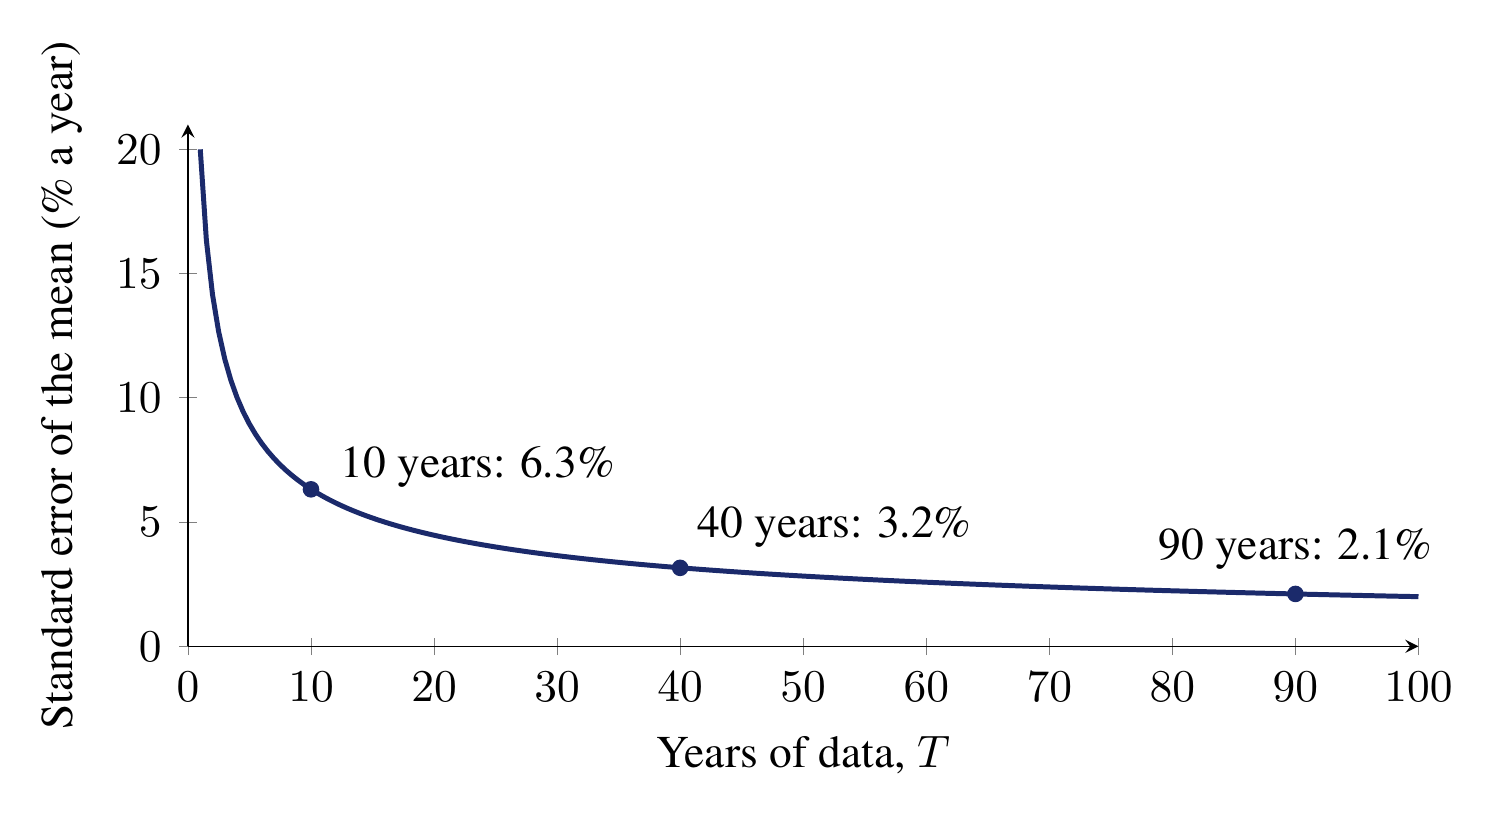
\includegraphics[width=0.85\linewidth]{images/fig19-1-se-years.png}
\caption{The standard error of an average return with 20\% volatility. With ten years of data it is 6.3\% a year; even 90 years leave it at 2.1\%. Differences in expected return between similar assets are far smaller than this, so the optimizer's most important input is mostly noise.}
\label{fig:19-se}
\end{figure}

\textbf{Worked example.} Two assets each have 20\% volatility and correlation 0.5. Asset A is expected to earn 8\% over bills and asset B 6\%. The tangency weights are proportional to $\boldsymbol{\Sigma}^{-1}\boldsymbol{\mu}$, which is proportional to $(0.08 - 0.5 \times 0.06,\; 0.06 - 0.5 \times 0.08) = (0.05,\; 0.02)$. Scaled to sum to 1, that is 71\% in A and 29\% in B.

\begin{itemize}
  \item Suppose the estimates were swapped, A at 6\% and B at 8\%. That is a 2-point error, a third of one standard error. The weights flip to 29\% in A and 71\% in B.
  \item {\sloppy If the correlation is 0.9 instead of 0.5, the original estimates give $(0.08 - 0.054,\; 0.06 - 0.072) = (0.026,\; -0.012)$: \textbf{186\% in A and $-86\%$ in B}.\par}
\end{itemize}

The more alike the assets, the more the optimizer bets on small differences in their estimated returns (Figure~\ref{fig:19-weights}).

\begin{figure}[htbp]
\centering
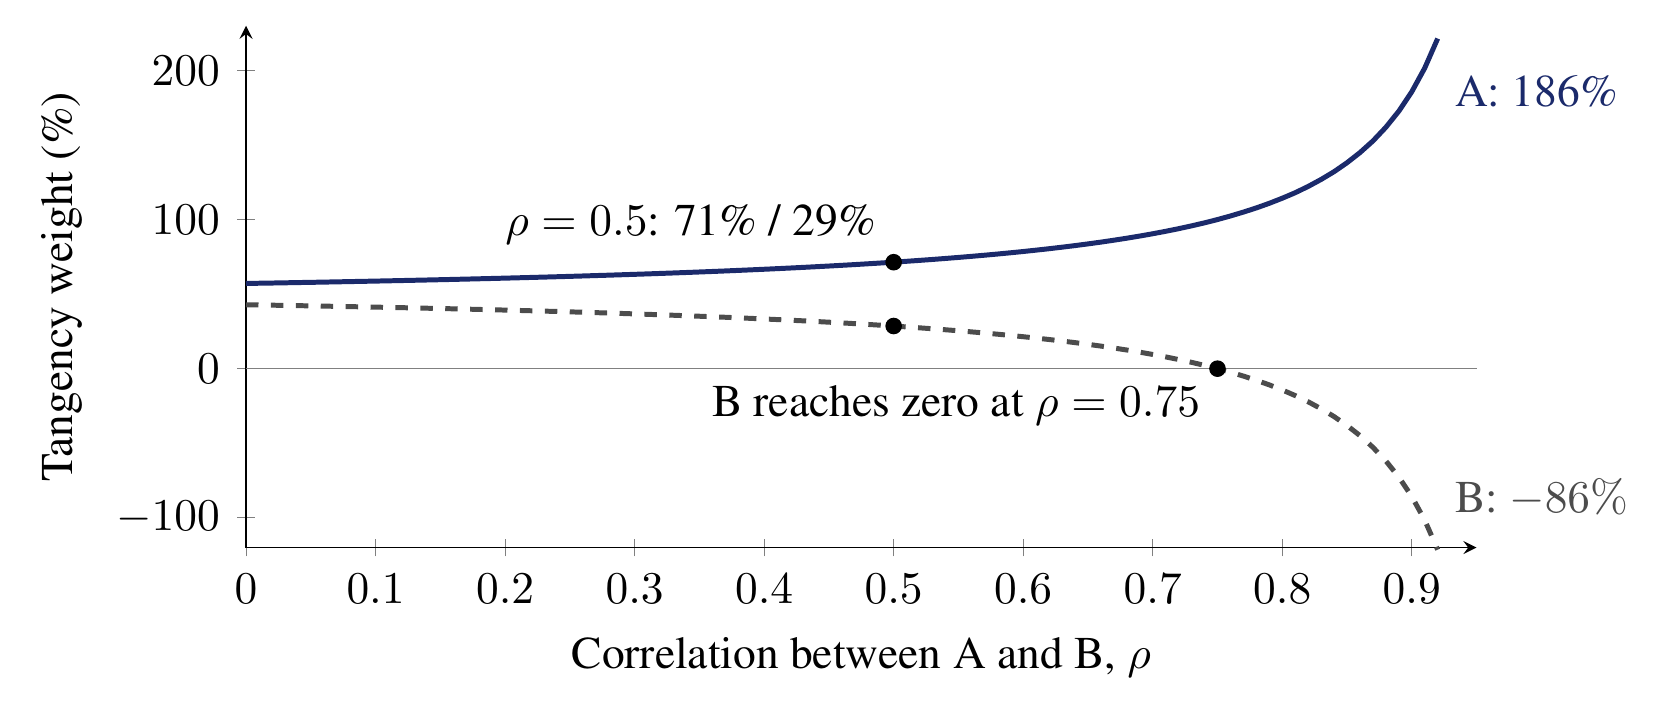
\includegraphics[width=0.85\linewidth]{images/fig19-2-weights-corr.png}
\caption{Tangency weights in the worked example as the correlation between the two assets rises, with expected returns fixed at 8\% and 6\%. At a correlation of 0.5 the split is 71/29; B's weight reaches zero at 0.75; at 0.9 the optimizer holds 186\% in A and shorts 86\% of B.}
\label{fig:19-weights}
\end{figure}

\textbf{Equal weighting (1/N)} puts $1/N$ in each asset. It uses no estimates, so it has no estimation error. It is optimal only if all assets have the same expected return, the same variance and the same pairwise correlations, but it never makes a large mistake.

\textbf{Repairs.} Four families of methods try to keep what optimization gets right while limiting estimation error:

\begin{itemize}
  \item \textbf{Constraints.} Ruling out short sales ($\mathbf{w} \geq 0$) caps the damage a bad estimate can do.
  \item \textbf{Shrinkage.} The Ledoit--Wolf estimator pulls the sample covariance $\mathbf{S}$ toward a simple target $\mathbf{F}$, with the intensity $\delta$ chosen from the data:
  \begin{equation}
    \hat{\boldsymbol{\Sigma}} = \delta\mathbf{F} + (1 - \delta)\mathbf{S}
    \label{eq:19-shrink}
  \end{equation}
  \item \textbf{Ignoring means.} Minimum-variance and risk-based rules drop $\boldsymbol{\mu}$, the noisiest input.
  \item \textbf{Risk budgeting.} Each asset's \textbf{risk contribution} is
  \begin{equation}
    RC_i = \frac{w_i\,(\boldsymbol{\Sigma}\mathbf{w})_i}{\sigma_p}
    \label{eq:19-rc}
  \end{equation}
  and the contributions sum to the portfolio volatility $\sigma_p$. \textbf{Equal risk contribution} sets them equal (Maillard, Roncalli and Teiletche 2010). \textbf{Inverse-volatility weighting} does so exactly when all correlations are equal.
\end{itemize}

\textbf{Judging out of sample.} Portfolios are formed from past data only and judged on the returns that follow. Two measures recur:

\begin{itemize}
  \item the Sharpe ratio;
  \item the \textbf{certainty equivalent}, the risk-free return the investor would accept instead:
  \begin{equation}
    CE = \mu_p - \frac{\gamma}{2}\,\sigma_p^2
    \label{eq:19-ce}
  \end{equation}
\end{itemize}

The \textbf{Jobson--Korkie test} (Jobson and Korkie 1981), with Memmel's (2003) correction, checks whether two Sharpe ratios differ by more than chance.

\textbf{Further reading.} Bodie, Kane and Marcus, \emph{Investments} (optimal risky portfolios and the efficient frontier); Cochrane, \emph{Asset Pricing} (the mean-variance problem in a modern asset-pricing framework); Campbell and Viceira, \emph{Strategic Asset Allocation}, and Meucci, \emph{Risk and Asset Allocation} (estimation error, Bayesian methods and long-horizon allocation); Roncalli, \emph{Introduction to Risk Parity and Budgeting}; Grinold and Kahn, \emph{Active Portfolio Management} (practitioner portfolio construction and transaction costs).

\section{How it works}
\label{sec:19-how}

In theory the mean-variance portfolio is the best one can do: no other mix of the same assets has a higher expected Sharpe ratio. In practice the optimizer is fed estimates, and it cannot tell signal from noise. Richard Michaud (1989) put the problem bluntly. Mean-variance optimization tends to maximize the effects of errors in its inputs, so that unconstrained optimized portfolios can do worse than equal weighting. Fischer Black and Robert Litterman (1992), writing from Goldman Sachs, described quantitative allocation models as difficult to use and prone to producing ``badly behaved'' portfolios.

The mechanism is in the inverse covariance matrix. $\boldsymbol{\Sigma}^{-1}$ magnifies differences between similar assets, as the worked example showed. Ten industry portfolios are all highly correlated with the market, so $\boldsymbol{\Sigma}^{-1}\boldsymbol{\mu}$ is dominated by small, noisy differences in their estimated means. The result is large long and short positions that change sharply from one month to the next. Each change costs money to trade.

The repairs attack different parts of the problem:

\begin{itemize}
  \item \textbf{Drop the means.} Minimum-variance portfolios use only $\boldsymbol{\Sigma}$. They usually lower volatility, but they still invert a noisy matrix and can hold large short positions.
  \item \textbf{Constrain the weights.} Jagannathan and Ma (2003) showed that a no-short-sale constraint is equivalent to shrinking the largest elements of the sample covariance matrix. It helps even when the true optimal portfolio would hold short positions.
  \item \textbf{Shrink the estimates.} Ledoit and Wolf (2004) shrink the sample covariance toward a scaled identity matrix. Black and Litterman (1992) shrink expected returns toward those implied by market equilibrium.
  \item \textbf{Avoid inversion.} Inverse-volatility weighting and equal risk contribution need only volatilities and correlations. \textbf{Hierarchical risk parity} (L\'opez de Prado 2016) clusters assets by correlation and splits capital down the resulting tree, never inverting $\boldsymbol{\Sigma}$.
  \item \textbf{Trade less.} Rebalancing less often, or penalizing turnover, cuts costs at the price of holding stale weights.
\end{itemize}

Each repair moves the portfolio closer to 1/N. That is the central tension of this chapter: the more an optimizer is protected from estimation error, the more it resembles the rule it was meant to beat.

\section{The claim}
\label{sec:19-claim}

\begin{callout}
\textbf{Claim.} Optimized portfolios deliver better out-of-sample risk-adjusted returns than simple rules such as equal weighting.
\end{callout}

The claim comes in two strengths:

\begin{itemize}
  \item \textbf{The strong form} is that classic mean-variance optimization, fed with sample estimates, beats 1/N out of sample.
  \item \textbf{The weak form} is that some disciplined form of optimization beats 1/N reliably, after trading costs. That form might be constrained, shrunk, risk-based or clustered.
\end{itemize}

To count as evidence, a result must:

\begin{itemize}
  \item use only data available at each rebalancing date;
  \item report the Sharpe ratio or certainty equivalent net of realistic costs;
  \item show that the gap over 1/N is larger than chance would produce;
  \item hold across more than one set of assets.
\end{itemize}

\section{The original evidence}
\label{sec:19-evidence}

\textbf{The theory (Markowitz 1952).} Markowitz's paper proves that the mean-variance portfolio is optimal when means and covariances are known. It contains no test, because there is nothing to test in sample. The optimized portfolio always wins on the data used to build it.

\textbf{The warnings (Michaud 1989; Black and Litterman 1992; Chopra and Ziemba 1993).} Practitioners reported early that optimized portfolios were concentrated, unstable and hard to justify to clients. Chopra and Ziemba ranked the damage done by errors in each input and found errors in means to be the most harmful by far. That finding is the reason minimum-variance and risk-based rules exist.

\textbf{The repairs work in their own tests.}

\begin{itemize}
  \item Jagannathan and Ma (2003) found that long-only minimum-variance portfolios built from monthly sample covariances performed about as well as those built from factor models, shrinkage estimators or daily data.
  \item Ledoit and Wolf (2004) derived the optimal shrinkage intensity and showed that the shrunk matrix is well conditioned even when assets outnumber observations.
  \item L\'opez de Prado (2016) reported that hierarchical risk parity delivered lower out-of-sample variance than Markowitz's critical-line algorithm, even though minimum variance is that algorithm's own objective. The evidence in the paper's abstract comes from Monte Carlo experiments, not from market data.
\end{itemize}

\textbf{The challenge (DeMiguel, Garlappi and Uppal 2009).} DeMiguel, Garlappi and Uppal (DGU) evaluated fourteen models across seven empirical datasets, on Sharpe ratio, certainty equivalent and turnover. None was consistently better than 1/N. Their models included:

\begin{itemize}
  \item sample mean-variance;
  \item Bayesian and Bayes--Stein estimators;
  \item minimum variance;
  \item constrained versions of each;
  \item mixtures of several rules.
\end{itemize}

They then asked how long an estimation window would be needed for sample mean-variance to beat 1/N. Their answer was around 3,000 months for 25 assets and about 6,000 months for 50, compared with roughly 1,100 months of U.S. stock data available today.

\textbf{The response (Kirby and Ostdiek 2012).} Kirby and Ostdiek argued that DGU's design favoured 1/N by focusing on portfolios with high estimation risk and extreme turnover. In their tests, standard mean-variance often beat 1/N before costs, but high turnover eroded the advantage. Two simple strategies, \textbf{volatility timing} and \textbf{reward-to-risk timing}, beat 1/N even with high transaction costs. Volatility timing weights assets by inverse variance; reward-to-risk timing weights by the ratio of mean to variance. Both ignore correlations and trade little.

The literature therefore agrees on the strong form: sample mean-variance loses to 1/N. It disagrees on the weak form, and the disagreement turns on costs, turnover and which assets are used.

\section{Replication lab: nine allocation rules against 1/N}
\label{sec:19-lab}

\begin{callout}
\textbf{Lab 19 at a glance.} \emph{Claim on trial:} optimized portfolios beat equal weighting out of sample. \emph{Data:} 10 and 30 industry portfolios and 25 size/book-to-market portfolios from the Kenneth R. French Data Library, with the risk-free rate; free. \emph{Code:} runs as a script (\texttt{python lab19.py}) or as a notebook (\texttt{lab19\_walkthrough.ipynb}) with a prediction prompt before each step.
\end{callout}

Lab 19 runs nine allocation rules walk-forward (Chapter 5). Each month, every rule is estimated on the previous 120 months of value-weighted excess returns and held for one month. Turnover is measured against the weights after they have drifted with that month's returns.

\begin{center}
\small
\begin{tabularx}{0.9\linewidth}{@{}>{\raggedright\arraybackslash}p{0.38\linewidth}>{\raggedright\arraybackslash}X@{}}
\toprule
Rule & What it estimates \\
\midrule
1/N & Nothing \\
Mean-variance (sample) & Means and covariance; scaled to sum to 1, gross exposure capped at 5 \\
Mean-variance, long-only & Means and covariance; risk aversion 5, weights 0 to 1 \\
Minimum variance (sample) & Covariance \\
Minimum variance, long-only & Covariance \\
Minimum variance, Ledoit--Wolf & Shrunk covariance \\
Risk parity (inverse volatility) & Volatilities \\
Equal risk contribution & Covariance \\
Hierarchical risk parity & Correlation clusters and variances \\
\bottomrule
\end{tabularx}
\end{center}

The lab has four parts:

\begin{itemize}
  \item \textbf{Part A} runs all nine rules on the 10 industry portfolios. It reports the Sharpe ratio, the certainty equivalent with $\gamma = 1$, turnover, extreme weights and maximum drawdown. Each rule is tested against 1/N with the Jobson--Korkie--Memmel test (Figures 19.3 and 19.4).
  \item \textbf{Part B} repeats the comparison on 30 industries and on 25 size/book-to-market portfolios, net of 25 basis points per unit of turnover (Figure 19.5).
  \item \textbf{Part C} varies the estimation window (60, 120, 240 months), costs (0, 25, 50 bp) and rebalancing frequency (1, 3, 12 months), and reports returns in three crises (Figure 19.6).
  \item \textbf{Part D} measures how unstable each rule's weights are: gross exposure, the largest weight, the share of short positions and month-to-month weight changes (Figure 19.7).
\end{itemize}

{\sloppy The option \texttt{-{}-fast} drops the three slower constrained rules, and \texttt{python lab19.py -{}-source sim} tests the code on simulated data.\par}

\textbf{What the simulated run shows.} The lab was run end to end only on simulated data. In the simulation every asset has a similar true Sharpe ratio, so 1/N is close to optimal by construction. The results show that the code behaves as theory predicts, not what real markets do.

\begin{itemize}
  \item On ten simulated assets, 1/N earned a Sharpe ratio of 0.44. Sample mean-variance earned 0.30, with average gross exposure of 4.1 and turnover of 74\% a month.
  \item Inverse volatility, equal risk contribution and hierarchical risk parity all landed between 0.44 and 0.45. None differed from 1/N significantly.
  \item Sample minimum variance cut volatility from 16\% to 12\% but earned a lower Sharpe ratio (0.40). Ledoit--Wolf shrinkage recovered most of the gap (0.43).
  \item With 30 or 25 assets, estimation error grew. After costs, sample mean-variance fell to Sharpe ratios of 0.15 and 0.25, and sample minimum variance fell to 0.07 and 0.10. Both were significantly worse than 1/N.
  \item A 240-month window lifted sample mean-variance to 0.44, close to 1/N, and cut its turnover by a third.
\end{itemize}

Run on real data, the lab will answer the question the simulation cannot: whether real assets differ enough in expected return and risk for optimization to earn back its estimation error.

\section{Stress tests}
\label{sec:19-stress}

\textbf{Estimation window.} DGU's critical window for 25 assets, about 3,000 months, is far longer than any real sample. Longer windows reduce estimation noise but use older data, which may no longer describe today's markets. Part C shows how the ranking changes as the window grows from five to twenty years.

\textbf{Trading costs.} Optimized rules trade far more than 1/N. In the simulated run, sample mean-variance turned over 74\% of the portfolio each month, against 3\% for 1/N. At 25 bp per unit of turnover, that difference alone costs about 2\% a year. Any claimed gain from optimization should be judged net of costs at the scale the investor actually trades (Chapter 6).

\textbf{Rebalancing frequency.} Rebalancing quarterly or annually cuts turnover. The weights are then estimated on older data, so the reduction is not free. Part C reports whether the trade-off helps the optimized rules more than 1/N.

\textbf{Asset set.} Optimization should do best when assets differ most. Industry and size/book-to-market portfolios are already diversified and highly correlated with the market, which makes $\boldsymbol{\Sigma}$ nearly singular. Asset classes with genuinely different risks, such as stocks, bonds and commodities, give optimization more to work with. Individual stocks give it less, because the number of parameters grows with the square of the number of assets.

\textbf{Crises.} Minimum-variance portfolios tend to lose less in sell-offs, because they tilt toward low-volatility assets. Part C reports returns in the 2008 crisis, the 2020 crash and 2022 for each rule. A smaller loss in a crisis is a real benefit to some investors even if the Sharpe ratio over the whole sample is no higher.

\textbf{Statistical power.} Sharpe ratios estimated over 90 years still have standard errors of roughly 0.1. A rule would need a large edge over 1/N for the difference to be detectable. Failing to reject equality is not proof that two rules are equally good.

\section{Verdict}
\label{sec:19-verdict}

\begin{callout}
\textbf{Verdict: fails} (as of October 2026). In its plain form the claim fails. Sample mean-variance optimization, the method the claim is built on, does not beat equal weighting out of sample in the published evidence. DGU's estimate of the data needed for it to win, about 3,000 months for 25 assets, exceeds any real sample by a wide margin.
\end{callout}

The repaired versions do better but do not rescue the claim:

\begin{itemize}
  \item Constrained and shrunk minimum-variance portfolios reliably lower volatility. They do not reliably raise the Sharpe ratio above 1/N.
  \item Risk-based rules (inverse volatility, equal risk contribution, hierarchical risk parity) tend to tie with 1/N, which they closely resemble when assets have similar risks.
  \item Kirby and Ostdiek's timing rules are the strongest case for the weak form. They succeed by ignoring correlations and trading little, which is to say by giving up most of what makes optimization optimization.
\end{itemize}

The verdict would change if the lab, run on real data, showed a disciplined optimizer beating 1/N significantly, net of costs, across all three asset sets.

\section{What investors can use}
\label{sec:19-investors}

\begin{itemize}
  \item \textbf{Treat 1/N as the benchmark.} Any optimized allocation should be compared with equal weighting of the same assets, out of sample and net of costs. A strategy that cannot beat it is adding complexity, not value.
  \item \textbf{Distrust the expected-return inputs most.} If an optimizer's output changes sharply when an expected return moves by a percentage point, the output reflects the input, not the market.
  \item \textbf{Use optimization for risk, not return.} Minimum-variance and risk-budgeting tools do what they promise, lowering volatility or balancing risk, without relying on forecasts of returns.
  \item \textbf{Count the turnover.} A gain of a few tenths of a percent a year disappears quickly at 70\% monthly turnover.
  \item \textbf{Prefer constraints you can explain.} Position limits and no-short rules work partly because they are crude.
\end{itemize}

\textbf{Questions to ask a manager who sells optimized portfolios:}

\begin{itemize}
  \item How does the strategy compare with 1/N on the same assets, out of sample and after costs?
  \item Where do the expected returns come from, and how sensitive are the weights to them?
  \item How many parameters are estimated, and from how many observations?
  \item What is the average monthly turnover, and what cost per trade is assumed?
  \item Which constraints are imposed, and how much of the performance comes from them rather than from the optimizer?
\end{itemize}

\begin{callout}
\textbf{What Failed: the optimizer nobody would use.} In the early 1990s Fischer Black and Robert Litterman, working in Goldman Sachs's fixed-income division, reported that quantitative asset-allocation models had not played the important role in global portfolio management that their logic deserved. Investment professionals found the models difficult to use, and the portfolios they produced were ``badly behaved'': concentrated, extreme and sensitive to small changes in inputs. Black and Litterman's fix was to stop trusting historical means. They started from the expected returns implied by market equilibrium and let managers tilt away only where they had confident views. Michaud reached the same diagnosis from the other side: unconstrained optimization maximizes the effects of errors in its inputs. The lesson has outlived both papers. The optimizer works exactly as designed; the problem is what it is fed.
\end{callout}

\section{Open questions}
\label{sec:19-open}

\begin{itemize}
  \item \textbf{Many assets.} With hundreds of stocks, sample covariance matrices become singular. Do newer nonlinear shrinkage and factor-based estimators make large-scale optimization competitive with 1/N?
  \item \textbf{Machine-learning allocations.} Do methods that learn weights directly from data avoid estimation error, or simply hide it in more parameters? Chapter 21 takes up the general question.
  \item \textbf{Cost-aware optimization.} Optimizing net of trading costs, with turnover penalties, changes both the weights and the comparison. How much of DGU's result survives?
  \item \textbf{Diversification in stress.} Risk-based portfolios depend on correlations staying stable. Chapter 20 asks what happens when they do not.
\end{itemize}

\section*{Exercises}
\addcontentsline{toc}{section}{Exercises}

\subsection*{Conceptual (all readers)}

\begin{enumerate}
  \item Two assets have volatilities of 15\% and 25\% and correlation 0.3. Compute the global minimum-variance weights. Then compute the inverse-volatility weights. Which portfolio has lower variance, and by how much?
  \item Using the worked example in Section~\ref{sec:19-foundations}, find the correlation at which the tangency portfolio first takes a short position in asset B, with expected returns of 8\% and 6\%.
  \item An asset has 18\% volatility. How many years of data are needed for the standard error of its mean return to fall below 1\% a year? What does this imply for estimating the difference in mean returns between two industries?
\end{enumerate}

\subsection*{Lab extensions (technical readers)}

\begin{enumerate}
  \setcounter{enumi}{3}
  \item Part A: run on real data. Which rules beat 1/N on Sharpe ratio, and are any differences significant at the 5\% level?
  \item Re-run with \texttt{-{}-window 240} and \texttt{-{}-window 360}. How quickly does sample mean-variance approach 1/N?
  \item Part B: compare the gap between sample minimum variance and its Ledoit--Wolf version on 10, 30 and 25 assets. Why does shrinkage matter more with more assets?
  \item Add a rule that holds half 1/N and half minimum variance, Ledoit--Wolf. Does the mixture beat both parts?
  \item Kirby and Ostdiek argue that DGU's design favoured 1/N. DGU might reply that real investors face exactly that estimation risk. Who has the better of the argument, and what evidence would settle it?
  \item A pension fund holds stocks, bonds, real estate and commodities. Would you expect optimization to do better relative to 1/N for this fund than for a portfolio of ten U.S. industries? Explain.
\end{enumerate}

\section*{References}
\addcontentsline{toc}{section}{References}

\begin{itemize}
  \item Black, F. and Litterman, R. (1992). Global Portfolio Optimization. \emph{Financial Analysts Journal} 48(5): 28--43.
  \item Chopra, V. K. and Ziemba, W. T. (1993). The Effect of Errors in Means, Variances, and Covariances on Optimal Portfolio Choice. \emph{Journal of Portfolio Management} 19(2): 6--11.
  \item DeMiguel, V., Garlappi, L. and Uppal, R. (2009). Optimal versus Naive Diversification: How Inefficient Is the 1/N Portfolio Strategy? \emph{Review of Financial Studies} 22(5): 1915--1953.
  \item Jagannathan, R. and Ma, T. (2003). Risk Reduction in Large Portfolios: Why Imposing the Wrong Constraints Helps. \emph{Journal of Finance} 58(4): 1651--1684.
  \item Jobson, J. D. and Korkie, B. M. (1981). Performance Hypothesis Testing with the Sharpe and Treynor Measures. \emph{Journal of Finance} 36(4): 889--908.
  \item Kirby, C. and Ostdiek, B. (2012). It's All in the Timing: Simple Active Portfolio Strategies That Outperform Naive Diversification. \emph{Journal of Financial and Quantitative Analysis} 47(2): 437--467.
  \item Ledoit, O. and Wolf, M. (2004). A Well-Conditioned Estimator for Large-Dimensional Covariance Matrices. \emph{Journal of Multivariate Analysis} 88(2): 365--411.
  \item L\'opez de Prado, M. (2016). Building Diversified Portfolios That Outperform Out of Sample. \emph{Journal of Portfolio Management} 42(4): 59--69.
  \item Maillard, S., Roncalli, T. and Teiletche, J. (2010). The Properties of Equally Weighted Risk Contribution Portfolios. \emph{Journal of Portfolio Management} 36(4): 60--70.
  \item Markowitz, H. (1952). Portfolio Selection. \emph{Journal of Finance} 7(1): 77--91.
  \item Memmel, C. (2003). Performance Hypothesis Testing with the Sharpe Ratio. \emph{Finance Letters} 1: 21--23.
  \item Michaud, R. O. (1989). The Markowitz Optimization Enigma: Is ``Optimized'' Optimal? \emph{Financial Analysts Journal} 45(1): 31--42.
\end{itemize}

\textbf{Data:} Kenneth R. French Data Library: 10 and 30 Industry Portfolios; 25 Portfolios Formed on Size and Book-to-Market; Fama/French 3 Factors (risk-free rate).

% Chapter 20 -- Claim: Diversification Fails When You Need It Most
% Requires: amsmath, amssymb, booktabs, array, tabularx, graphicx, tcolorbox (breakable, skins), hyperref or url.
% Defines the callout box only if the preamble has not.
\providecolor{fenavy}{HTML}{1B2A6B}
\providecolor{feshade}{HTML}{F3F5FA}
\makeatletter
\@ifundefined{callout}{%
  \newtcolorbox{callout}{breakable, enhanced,
    colback=white, colframe=gray!70, boxrule=0.5pt, arc=1mm,
    borderline west={2.5pt}{0pt}{gray!70},
    left=8pt, right=8pt, top=4pt, bottom=4pt}%
}{}
\makeatother

\chapter{Claim: Diversification Fails When You Need It Most}
\label{ch:20}

Diversification is often called the only free lunch in finance. Combine assets that do not move in lockstep, and the portfolio's risk falls below the average risk of its parts at no cost in expected return. Every balanced fund, target-date fund and pension portfolio rests on that arithmetic.

A common complaint is that the free lunch is withdrawn just when it is needed. In 1987, 2008 and March 2020, almost everything risky fell at once. Correlations measured in calm years seemed to jump toward one, and investors who thought they were diversified found that they were not. In 2022, even Treasury bonds, the traditional shelter, fell alongside stocks.

This chapter tests whether that complaint is a fact about markets or partly an artefact of how correlations are measured in turbulent times.

By the end of the chapter you will be able to:

\begin{itemize}
  \item compute portfolio volatility from correlations, and explain why average correlation sets a floor on diversification;
  \item measure the diversification ratio;
  \item explain why measured correlation rises with volatility, and apply the Forbes--Rigobon correction;
  \item interpret exceedance correlations and tail dependence against a normal benchmark;
  \item explain why the stock--bond correlation changes sign with the inflation regime;
  \item separate the statistical claim (correlations rise in crises) from the economic one (diversified portfolios fail), and judge a portfolio by its losses in bad months.
\end{itemize}

\section{Foundations: correlation, diversification and how crisis correlations are measured}
\label{sec:20-foundations}

\textbf{Correlation and diversification.} For two assets with weights $w_1$ and $w_2$, volatilities $\sigma_1$ and $\sigma_2$ and correlation $\rho$, portfolio variance is
\begin{equation}
  \sigma_p^2 = w_1^2\sigma_1^2 + w_2^2\sigma_2^2 + 2w_1w_2\rho\,\sigma_1\sigma_2
  \label{eq:20-var2}
\end{equation}
The lower the correlation, the lower the portfolio's risk. With $N$ assets of equal volatility $\sigma$ and equal pairwise correlation $\rho$, an equally weighted portfolio has variance
\begin{equation}
  \sigma_p^2 = \sigma^2\left[\rho + \frac{1 - \rho}{N}\right]
  \label{eq:20-varN}
\end{equation}
As $N$ grows, the variance falls toward $\rho\sigma^2$. The average correlation therefore sets a floor on how much risk diversification can remove (Figure~\ref{fig:20-floor}). The \textbf{diversification ratio}, the weighted average of the assets' volatilities divided by the portfolio's volatility, measures the benefit. A ratio of 1 means none.

\textbf{Worked example.} Ten industries each have 20\% volatility. At an average correlation of 0.6, an equally weighted portfolio has volatility $20\% \times \sqrt{0.6 + 0.4/10} = 16.0\%$. If the correlation rises to 0.8, the volatility rises to $20\% \times \sqrt{0.8 + 0.2/10} = 18.1\%$. A rise in correlation of that size wipes out half of the diversification benefit, from 4 points of volatility to under 2.

\begin{figure}[htbp]
\centering
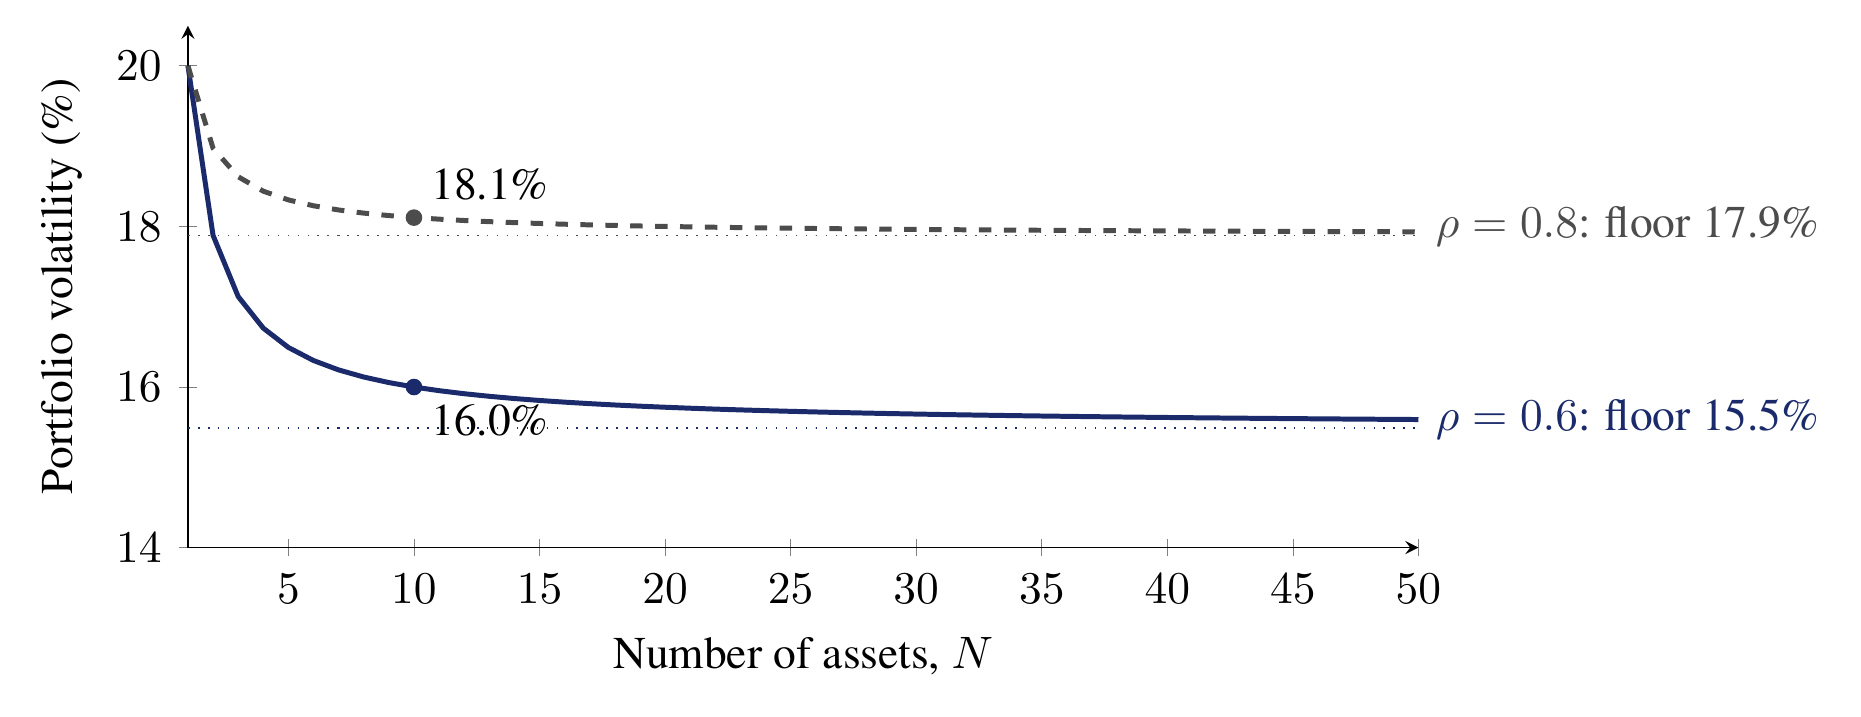
\includegraphics[width=0.85\linewidth]{images/fig20-1-div-floor.png}
\caption{Volatility of an equally weighted portfolio of assets with 20\% volatility each. Adding assets helps only down to a floor set by the average correlation: 15.5\% at a correlation of 0.6 and 17.9\% at 0.8. With ten assets, as in the worked example, a rise from 0.6 to 0.8 lifts volatility from 16.0\% to 18.1\%.}
\label{fig:20-floor}
\end{figure}

\textbf{Why measured correlation rises when volatility rises.} Suppose $y = \beta x + e$, with the noise $e$ unchanged when $x$ becomes more volatile. The correlation of $x$ and $y$ is
\begin{equation}
  \rho = \frac{\beta\sigma_x}{\sqrt{\beta^2\sigma_x^2 + \sigma_e^2}}
  \label{eq:20-bias}
\end{equation}
which rises with $\sigma_x$ even though the link between the two markets, $\beta$, has not changed (Figure~\ref{fig:20-bias}). Correlations measured in turbulent periods are therefore \textbf{biased upward} (Boyer, Gibson and Loretan 1999).

\begin{figure}[htbp]
\centering
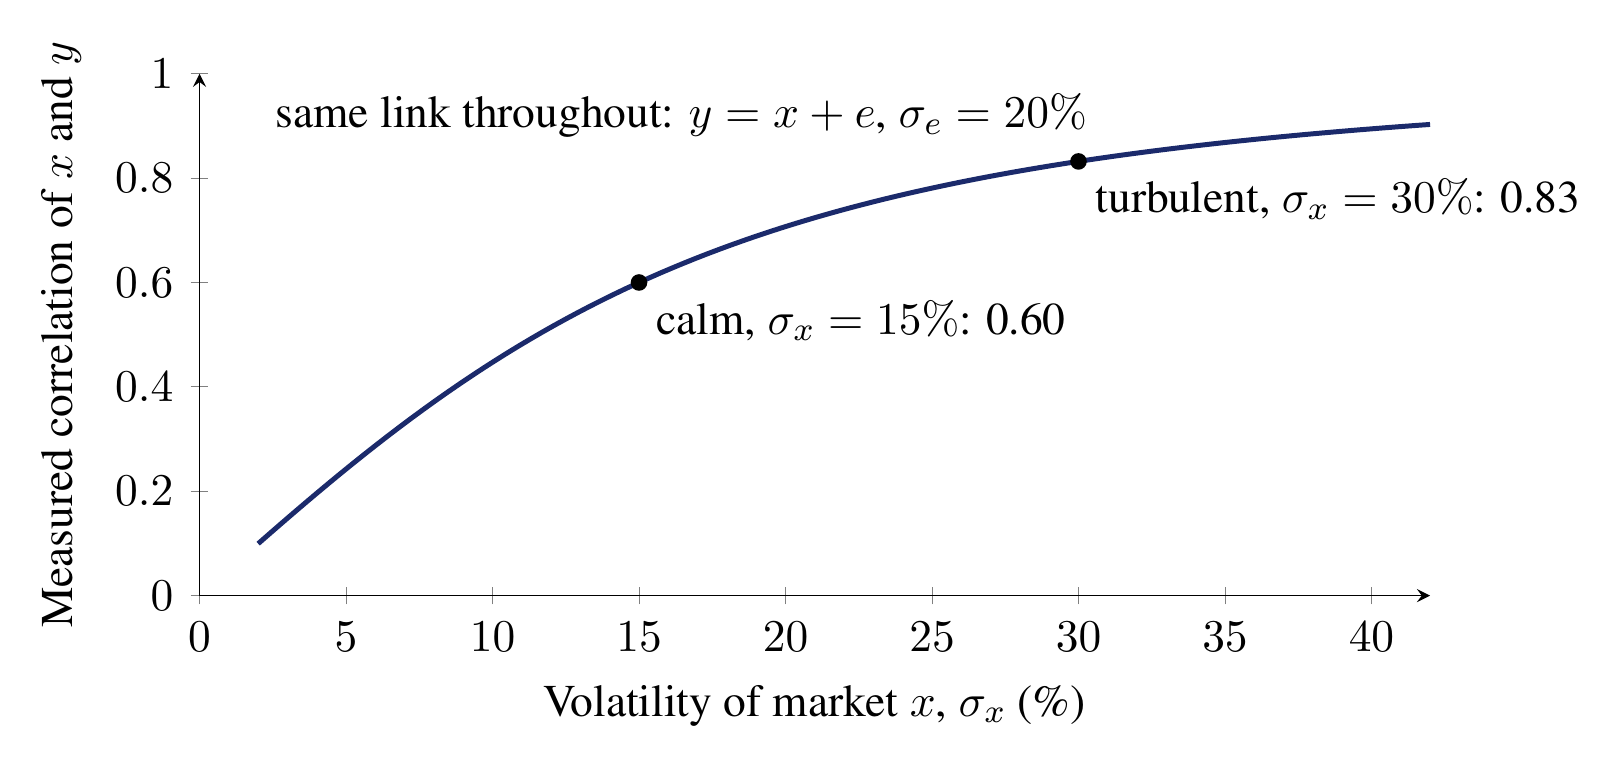
\includegraphics[width=0.85\linewidth]{images/fig20-2-vol-bias.png}
\caption{The volatility bias in measured correlation. The link between the two markets never changes ($y = x + e$, with noise of 20\%), yet the measured correlation rises from 0.60 when $x$ has 15\% volatility to 0.83 when it has 30\%.}
\label{fig:20-bias}
\end{figure}

\textbf{The Forbes--Rigobon correction.} Forbes and Rigobon (2002) proposed a correction. If $\rho_c$ is the correlation measured in a period when the variance of $x$ is higher by a factor $1 + \delta$, the correlation that would hold at normal variance is
\begin{equation}
  \rho^* = \frac{\rho_c}{\sqrt{1 + \delta\,(1 - \rho_c^2)}}
  \label{eq:20-fr}
\end{equation}
For example, a crisis correlation of 0.8, measured when variance is four times its normal level ($\delta = 3$), corresponds to $0.8/\sqrt{1 + 3 \times 0.36} = 0.55$ in normal times. The correction assumes the extra volatility starts in $x$. If the link itself strengthens in crises, the correction removes part of a real change.

\textbf{Conditioning on the tails.} Truncating a sample also changes its correlation. For a bivariate normal distribution, the correlation among observations where both variables are below some threshold is lower than the full-sample correlation, and falls further as the threshold moves into the tail. \textbf{Exceedance correlations} (Longin and Solnik 2001; Ang and Chen 2002) are measured over observations where both returns are beyond a quantile, and are compared with what a normal distribution with the same overall correlation would produce. The gap between the two, not the raw level, is the evidence of asymmetry.

\textbf{Tail dependence} asks how likely one asset is to have an extreme loss when another does: $P(Y \text{ in its worst } p\text{-tail} \mid X \text{ in its worst } p\text{-tail})$. For independent assets the answer is $p$. For a normal distribution it falls toward $p$ as $p$ shrinks. Fat-tailed joint distributions, modelled with \textbf{copulas} (functions that join marginal distributions into a joint one) such as the Student $t$ or Clayton, keep it higher.

\textbf{The stock--bond correlation.} Government bonds hedge stocks when bad economic news lowers both expected profits and interest rates. They fail as hedges when inflation news dominates, because rising inflation hurts both bond prices and, through higher discount rates, stock prices. The sign of the stock--bond correlation has changed over the decades.

\textbf{Further reading.} Bodie, Kane and Marcus, \emph{Investments} (portfolio variance and diversification); Tsay, \emph{Analysis of Financial Time Series}, and Campbell, Lo and MacKinlay, \emph{The Econometrics of Financial Markets} (correlation dynamics and multivariate GARCH); McNeil, Frey and Embrechts, \emph{Quantitative Risk Management} (copulas, tail dependence and extreme value theory); Ang, \emph{Asset Management}, and Ilmanen, \emph{Expected Returns} (diversification, regimes and the stock--bond correlation from an investor's view).

\section{How it works}
\label{sec:20-how}

Three different things can make diversification look weaker in a crisis, and they have different implications for investors.

\begin{itemize}
  \item \textbf{A measurement effect.} When volatility rises, measured correlation rises even if the underlying relationship is unchanged. This part is an artefact, and correcting for it shrinks the apparent increase.
  \item \textbf{A common shock.} In a crisis, one factor, such as a global panic, a funding squeeze or a recession scare, comes to dominate returns. Assets that usually move on separate news now move on the same news. This is a real change, and it is the one that hurts investors.
  \item \textbf{A change of regime.} Some relationships flip sign with the economic environment. The stock--bond correlation is the main example: negative when growth shocks dominate, positive when inflation shocks dominate.
\end{itemize}

What matters to an investor is not the correlation itself but the return of the portfolio in bad times. A portfolio can lose less than stocks in a crash even if correlations rise, provided some assets fall less than others. Diversification fails in the investor's sense only when every holding falls about as much as the riskiest one.

The mechanisms also differ by asset. International stocks share the global equity factor, so their correlation with U.S. stocks is high to begin with and may rise further in sell-offs. Industries within one market are even more closely linked. Treasury bonds and commodities respond to different forces, and their link to stocks can change sign.

\section{The claim}
\label{sec:20-claim}

\begin{callout}
\textbf{Claim.} Correlations rise in crises, so diversification fails exactly when investors need it most.
\end{callout}

The claim has two parts, and each can be tested separately:

\begin{itemize}
  \item \textbf{The statistical part:} correlations between risky assets are higher in down markets and turbulent periods than in calm ones, by more than the volatility bias and the normal distribution would imply.
  \item \textbf{The economic part:} as a result, diversified portfolios offer little protection in the worst months.
\end{itemize}

The first part can be true while the second is false. That happens if diversifiers such as Treasury bonds keep their low or negative correlation with stocks while equity correlations rise.

\section{The original evidence}
\label{sec:20-evidence}

\textbf{International equity markets (Longin and Solnik 2001).} Using monthly returns for the U.S., the U.K., France, Germany and Japan from 1959 to 1996, Longin and Solnik applied extreme value theory to the tails of the joint distribution. They found that the correlation of large negative returns rises in bear markets but not in bull markets. Multivariate normality was rejected for the negative tail but not for the positive one. They concluded that the market's direction, not volatility alone, drives the increase. They also warned that simply conditioning on large absolute returns can create a spurious rise in correlation.

\textbf{U.S. stocks (Ang and Chen 2002).} Ang and Chen found that correlations between U.S. stock portfolios and the market are much greater for downside moves than for upside moves, especially extreme ones. Conditional on the downside, correlations in the data differed from those implied by a normal distribution by 11.6\%. Small stocks, value stocks and past losers showed the most asymmetry. Among the models they tried, regime-switching models captured the asymmetry best; GARCH models did poorly.

\textbf{Contagion or interdependence (Forbes and Rigobon 2002).} Forbes and Rigobon studied three crises: the 1987 U.S. crash, the 1994 Mexican peso collapse and the 1997 East Asian crisis. With unadjusted correlations, several countries showed evidence of \textbf{contagion}, meaning correlations that rose in the crisis. After correcting for the higher volatility, there was virtually none. They concluded that the high co-movement reflected strong linkages that existed all along, which they called \textbf{interdependence}.

\textbf{Investor-focused evidence (Page and Panariello 2018).} Using monthly data from 1970 to mid-2017, Page and Panariello reported that the correlation between U.S. and non-U.S. developed stocks was $-17\%$ during the strongest U.S. rallies and $+87\%$ during the worst 1\% of U.S. sell-offs. They found a similar pattern for real estate, corporate and high-yield bonds, emerging markets and hedge funds. Treasury bonds usually decoupled from stocks in sell-offs, but the authors noted that the stock--bond correlation can turn positive when inflation or interest rates drive markets. Their correlations are conditioned on U.S. returns alone, so part of the asymmetry may reflect the truncation effect described in Section~\ref{sec:20-foundations}.

\textbf{The stock--bond correlation (Campbell, Sunderam and Viceira 2017).} Campbell, Sunderam and Viceira found that the covariance between Treasury bond and stock returns was slightly positive on average over 1953 to 2009 but varied a great deal. It was unusually high in the early 1980s and negative in the 2000s, especially in the 2000--02 and 2007--09 downturns. They linked the change to how inflation and real rates co-move with the real economy.

The evidence supports the statistical part of the claim for equities, with caveats about measurement. It contradicts any simple version for bonds, whose hedging value depends on the inflation regime.

\section{Replication lab: correlations in calm and crisis}
\label{sec:20-lab}

\begin{callout}
\textbf{Lab 20 at a glance.} \emph{Claim on trial:} diversification fails when it is needed most. \emph{Data:} U.S. market excess returns from 1926, international developed-market returns from 1990 and 10 industry portfolios, all from the Kenneth R. French Data Library; the 10-year Treasury yield (GS10, from 1953), consumer prices (CPIAUCSL) and the spot oil price (WTISPLC) from FRED. All are free. \emph{Code:} runs as a script (\texttt{python lab20.py}) or as a notebook (\texttt{lab20\_walkthrough.ipynb}) with a prediction prompt before each step.
\end{callout}

Bond returns are built from yields by buying a 10-year par bond each month and selling it a month later at the new yield.

The lab has four parts:

\begin{itemize}
  \item \textbf{Part A} measures the correlation of U.S. stocks with international stocks, bonds and oil, and the average pairwise correlation of the ten industries. It reports each in calm months, in high-volatility months (the top fifth by trailing 12-month U.S. volatility), after the Forbes--Rigobon correction and in the worst 10\% of U.S. months. It also plots exceedance correlations against a normal benchmark (Figures 20.3 and 20.4).
  \item \textbf{Part B} measures tail dependence at the 5\%, 10\% and 20\% levels, against a normal distribution with the same correlation.
  \item \textbf{Part C} tracks the rolling 36-month stock--bond correlation and relates it to inflation. It reports results by decade and by inflation regime, and for 2022 (Figure 20.5).
  \item \textbf{Part D} compares 100\% stocks, a 60/40 stock--bond portfolio and an equal-weight mix of U.S. stocks, international stocks, bonds and oil. It reports average returns in the worst and best 5\% of stock months, drawdowns, five crisis periods and the diversification ratio (Figures 20.6 and 20.7).
\end{itemize}

The command \texttt{python lab20.py -{}-source sim} tests the code on simulated data.

\textbf{What the simulated run shows.} The lab was run end to end only on simulated data. The simulation was built so that the true correlation between U.S. and international stocks rises from 0.60 in calm regimes to 0.75 in stress, and so that the stock--bond correlation rises with inflation. The results test the code and illustrate the measurement problems; they say nothing about real markets.

\begin{itemize}
  \item The raw correlation between U.S. and international stocks rose from 0.61 in calm months to 0.70 in high-volatility months. The Forbes--Rigobon correction brought it down to 0.47, below the calm level, even though the simulation contained a true increase. The correction overshoots when the link itself strengthens in a crisis.
  \item In the worst 10\% of U.S. months, the same correlation was 0.45, lower than in calm months, because conditioning on one tail truncates the data.
  \item The average industry correlation rose from 0.68 to 0.80 in high-volatility months, and fell to 0.61 after correction.
  \item The stock--bond correlation was $-0.17$ when prior inflation was below 3\% and $+0.17$ when it was 3\% or more.
  \item In the worst 5\% of stock months, when stocks lost 8.5\% on average, the 60/40 portfolio lost 5.0\% and the equal-weight mix 4.7\%. The 60/40 diversification ratio fell from 1.26 in calm months to 1.16 in high-volatility months: smaller, but not zero.
\end{itemize}

On real data the lab answers the question the simulation cannot: whether the rise in correlations survives the correction, and whether diversified portfolios still cushioned the worst months.

\section{Stress tests}
\label{sec:20-stress}

\textbf{The definition of a crisis.} Results depend on how bad times are defined: high volatility, falling markets, recessions or a list of named crises. Correlations conditioned on direction (Longin and Solnik's bear markets) and on volatility (Forbes and Rigobon's turmoil) answer different questions. The lab offers both, and Exercise 4 adds recessions.

\textbf{The correction's assumption.} The Forbes--Rigobon adjustment assumes the extra volatility comes from the conditioning market and that the link between markets is fixed. If a crisis strengthens the link, the correction removes part of a real change, as the simulated run showed. The raw and corrected numbers are best read as upper and lower bounds.

\textbf{Frequency.} Monthly data smooth over the days when correlations spike. Daily correlations in October 1987 or March 2020 were higher than monthly ones. For a long-horizon investor, though, monthly or quarterly co-movement matters more than daily.

\textbf{Sample period.} International data begin in 1990, after the long era of capital controls ended. The stock--bond correlation depends heavily on whether the sample includes the high-inflation 1970s and early 1980s. A sample running from 2000 to 2021 shows bonds as a strong hedge; one including 1965--1985 or 2022 does not.

\textbf{Bond construction.} Returns built from constant-maturity yields approximate a bond index. They miss the coupon effects and roll of actual bonds but capture the duration risk that dominated 2022.

\textbf{Statistical power.} High-volatility months are a fifth of the sample, and extreme tails much less. With about 70 high-volatility months for international stocks, a correlation of 0.7 has a standard error near 0.06, so differences of a few hundredths are noise.

\section{Verdict}
\label{sec:20-verdict}

\begin{callout}
\textbf{Verdict: weakens} (as of October 2026). The statistical part of the claim holds for equities. Correlations among stock markets, and among industries within one market, are higher in falling markets than a normal distribution implies, and the asymmetry survives methods designed to avoid the volatility bias (Longin and Solnik 2001; Ang and Chen 2002). Part of the increase that investors notice in crises is a measurement effect, as Forbes and Rigobon showed, but not all of it. The economic part is overstated.
\end{callout}

\begin{itemize}
  \item \textbf{Diversifying across equities alone does fail in crises.} Adding international stocks or more industries buys little protection when it is most wanted.
  \item \textbf{Diversifying across asset classes has usually worked.} Treasury bonds rose in most stock-market crashes of the last forty years, and a 60/40 portfolio typically lost a fraction of what stocks lost in the worst months.
  \item \textbf{That protection is not a law.} It depends on the inflation regime. When inflation is high or rising, as in the 1970s and in 2022, stocks and bonds can fall together.
\end{itemize}

The claim is therefore true for the diversification most investors rely on least (within equities), and conditional for the diversification they rely on most (stocks and bonds). The verdict would move to \emph{survives} if real-data results showed stock--bond protection failing in growth-driven crises as well, and to \emph{fails} if equity correlations showed no asymmetry after correction.

\section{What investors can use}
\label{sec:20-investors}

\begin{itemize}
  \item \textbf{Use stress correlations, not average ones.} Plan with the correlations seen in the worst months, not the full-sample figure. For equities, assume they move closer together in a sell-off.
  \item \textbf{Diversify across risks, not labels.} Ten equity funds in different regions or styles are mostly one bet on the global equity factor. Real diversification needs assets driven by different forces, such as interest rates or inflation.
  \item \textbf{Know what your hedge hedges.} Long-term Treasury bonds hedge recessions and deflationary panics. They do not hedge inflation shocks. Cash, short-term bonds, inflation-linked bonds and some commodities behave differently.
  \item \textbf{Judge by portfolio losses.} Ask what the whole portfolio lost in past crises, not whether correlations rose.
  \item \textbf{Rebalance.} Diversified portfolios that rebalance sell what held up and buy what fell, which helps recoveries even when diversification disappointed in the fall.
\end{itemize}

\textbf{Questions to ask a manager or adviser:}

\begin{itemize}
  \item What did this portfolio lose in 2008, in March 2020 and in 2022?
  \item Which correlations do you use to estimate risk, and from which periods?
  \item Which of the holdings would be expected to rise if stocks fell 30\% because of a recession? And if they fell because of an inflation shock?
  \item How much of the portfolio's risk comes from the equity factor?
  \item Are any reported correlations based on smoothed or appraisal-based prices?
\end{itemize}

\begin{callout}
\textbf{What Failed: bonds as the hedge in 2022.} For most of the two decades before 2022, Treasury bonds rose when stocks fell, and the 60/40 portfolio became the default allocation. Then inflation reached its highest levels in forty years and the Federal Reserve raised rates rapidly. In 2022 the S\&P 500 fell 18.1\% and the U.S. dollar bond market about 13\%. According to Dimensional (Dimensional Fund Advisors 2023), a 60/40 portfolio lost 11\% over the year, with a drawdown of 19\% at its low point, and many bond indices had their worst year on record. Nothing in the correlation had been wrong; it had been estimated in a period dominated by growth shocks and low, stable inflation. When the dominant shock changed, so did the sign. Investors who treated a negative stock--bond correlation as a constant learned that it was a feature of a regime.
\end{callout}

\section{Open questions}
\label{sec:20-open}

\begin{itemize}
  \item \textbf{Which regime are we in?} Can the stock--bond correlation be forecast from inflation, inflation uncertainty or central-bank credibility well enough to adjust allocations in time?
  \item \textbf{Better crisis correlations.} Do regime-switching, copula or dynamic conditional correlation models forecast crisis co-movement out of sample, or only describe it after the fact?
  \item \textbf{Private assets.} Smoothed valuations make private equity and real estate look like diversifiers. How large is their true crisis correlation with public stocks?
  \item \textbf{New hedges.} Have trend-following, long-volatility or tail-hedging strategies delivered crisis protection at an acceptable cost? Chapter 14's evidence on option selling is the mirror image of this question.
\end{itemize}

\section*{Exercises}
\addcontentsline{toc}{section}{Exercises}

\subsection*{Conceptual (all readers)}

\begin{enumerate}
  \item Twenty assets each have 25\% volatility. Compute the volatility of an equally weighted portfolio when the average correlation is 0.3 and when it is 0.7. What share of the diversification benefit is lost?
  \item A correlation of 0.75 is measured in a crisis when the variance of the conditioning market is three times its normal level. Apply the Forbes--Rigobon correction. What correlation in normal times does it imply?
  \item Using $y = \beta x + e$ with $\beta = 0.6$, $\sigma_e = 15\%$ and $\sigma_x = 15\%$, compute the correlation of $x$ and $y$. Recompute with $\sigma_x = 30\%$. Explain why the correlation changed even though $\beta$ did not.
\end{enumerate}

\subsection*{Lab extensions (technical readers)}

\begin{enumerate}
  \setcounter{enumi}{3}
  \item Part A: run on real data. For which pairs does the high-volatility correlation exceed the calm one after the Forbes--Rigobon correction? Then define bad times as NBER recession months (FRED series USREC) instead of high-volatility months. Do the conclusions change?
  \item Compare the exceedance correlations of U.S. and international stocks with the normal benchmark (Figure 20.3). Is the gap larger in the lower tail than the upper tail?
  \item Part C: compute the stock--bond correlation for 1965--1985 and for 2000--2021. Relate the difference to average inflation in each period.
  \item Part D: list the five worst months for U.S. stocks since 1953. What did bonds do in each?
  \item Forbes and Rigobon say ``no contagion, only interdependence''. Why might an investor care little about the distinction?
  \item A client says, ``Bonds failed in 2022, so they are useless as a hedge.'' Using the chapter's evidence, write a short reply.
\end{enumerate}

\section*{References}
\addcontentsline{toc}{section}{References}

\begin{itemize}
  \item Ang, A. and Chen, J. (2002). Asymmetric Correlations of Equity Portfolios. \emph{Journal of Financial Economics} 63(3): 443--494.
  \item Boyer, B. H., Gibson, M. S. and Loretan, M. (1999). Pitfalls in Tests for Changes in Correlations. International Finance Discussion Paper 597, Board of Governors of the Federal Reserve System.
  \item Campbell, J. Y., Sunderam, A. and Viceira, L. M. (2017). Inflation Bets or Deflation Hedges? The Changing Risks of Nominal Bonds. \emph{Critical Finance Review} 6(2): 263--301.
  \item Dimensional Fund Advisors (2023). Market Review 2022: After a Down Year, Looking to the Past as a Guide.
  \item Forbes, K. J. and Rigobon, R. (2002). No Contagion, Only Interdependence: Measuring Stock Market Comovements. \emph{Journal of Finance} 57(5): 2223--2261.
  \item Longin, F. and Solnik, B. (2001). Extreme Correlation of International Equity Markets. \emph{Journal of Finance} 56(2): 649--676.
  \item Page, S. and Panariello, R. A. (2018). When Diversification Fails. \emph{Financial Analysts Journal} 74(3): 19--32.
\end{itemize}

\textbf{Data:} Kenneth R. French Data Library: Fama/French 3 Factors; Developed ex US 3 Factors; 10 Industry Portfolios. FRED, Federal Reserve Bank of St.\ Louis: 10-Year Treasury Constant Maturity Rate [GS10], Consumer Price Index [CPIAUCSL], Spot Crude Oil Price: WTI [WTISPLC].

% Chapter 21 -- Claim: Machine Learning Finds Hidden Alpha
% Requires: amsmath, amssymb, booktabs, array, tabularx, graphicx, tcolorbox (breakable, skins), hyperref or url.
% Defines the callout box only if the preamble has not.
\providecolor{fenavy}{HTML}{1B2A6B}
\providecolor{feshade}{HTML}{F3F5FA}
\makeatletter
\@ifundefined{callout}{%
  \newtcolorbox{callout}{breakable, enhanced,
    colback=white, colframe=gray!70, boxrule=0.5pt, arc=1mm,
    borderline west={2.5pt}{0pt}{gray!70},
    left=8pt, right=8pt, top=4pt, bottom=4pt}%
}{}
\makeatother

\chapter{Claim: Machine Learning Finds Hidden Alpha}
\label{ch:21}

Machine learning has transformed image recognition, translation and protein folding. The pitch to investors is that it can do the same for stock picking. Linear models, the argument runs, can only add up a handful of signals. Flexible models can find interactions and nonlinearities that humans never thought to look for, and with them, alpha that is hidden from everyone else.

The academic evidence gave the pitch real support. In 2020, Shihao Gu, Bryan Kelly and Dacheng Xiu reported that neural networks and regression trees roughly doubled the performance of leading regression-based strategies in predicting U.S. stock returns. Funds and ETFs branded with artificial intelligence followed.

Finance is a hard domain for machine learning. Signals are faint, data are short, and the patterns change as investors learn them. This chapter asks how much of the gain survives honest out-of-sample testing, realistic trading costs and the restriction to stocks that can actually be traded in size.

By the end of the chapter you will be able to:

\begin{itemize}
  \item state the return-prediction problem and describe the main model families: regularized regression, trees and ensembles, and neural networks;
  \item split data into training, validation and test samples in time order, and explain what each is for;
  \item measure success with the out-of-sample $R^2$, the Diebold--Mariano test and long--short portfolios, and explain why a tiny $R^2$ can be economically large;
  \item interpret a model with permutation importance, and explain the debate over the ``virtue of complexity'';
  \item state the three parts of the claim (statistical, hidden, economic) and summarize the evidence for each;
  \item judge a machine-learning strategy by its value-weighted, net-of-cost performance against a linear model on the same inputs.
\end{itemize}

\section{Foundations: supervised learning for return prediction}
\label{sec:21-foundations}

\textbf{The prediction problem.} For asset $i$ at the end of month $t$, a model maps a vector of characteristics $\mathbf{z}_{i,t}$, known at that time, to a forecast of next month's excess return:
\begin{equation}
  E_t[r_{i,t+1}] = g(\mathbf{z}_{i,t})
  \label{eq:21-g}
\end{equation}
Traditional models make $g$ linear, with a few characteristics chosen in advance. \textbf{Supervised machine learning} lets the data choose $g$ from a richer family and controls overfitting by holding back data to tune the model's complexity.

\textbf{The model families.}

\begin{itemize}
  \item \textbf{Ordinary least squares (OLS)} with many predictors fits noise. With $P$ predictors and $T$ observations, the in-sample fit improves mechanically with each added predictor.
  \item \textbf{Regularized regression} adds a penalty to the squared error. \textbf{Ridge} penalizes the sum of squared coefficients ($\lambda\sum_j\beta_j^2$), \textbf{lasso} the sum of their absolute values ($\lambda\sum_j|\beta_j|$), which sets some to zero, and the \textbf{elastic net} mixes the two.
  \item \textbf{Regression trees} split the data repeatedly on one characteristic at a time and predict the average return in each final group. A single tree overfits, so practitioners average many trees (\textbf{random forests}) or build them one after another, each correcting the last (\textbf{gradient boosting}). Tree depth controls how many characteristics can interact.
  \item \textbf{Neural networks} pass the inputs through layers of weighted sums and nonlinear functions. They can approximate almost any smooth function, but they have many parameters, depend on random initialization and need careful regularization: weight penalties, early stopping and averaging over several random \textbf{seeds}, the numbers that start the random initialization.
\end{itemize}

\textbf{Training, validation and testing.} The data are split in time (Figure~\ref{fig:21-split}). Models are fitted on a training sample, their tuning parameters (the penalty, the tree depth) are chosen on a later validation sample, and they are judged on a test sample that played no part in either step. Refitting as time passes keeps the split honest (Chapter 5).

\begin{figure}[htbp]
\centering
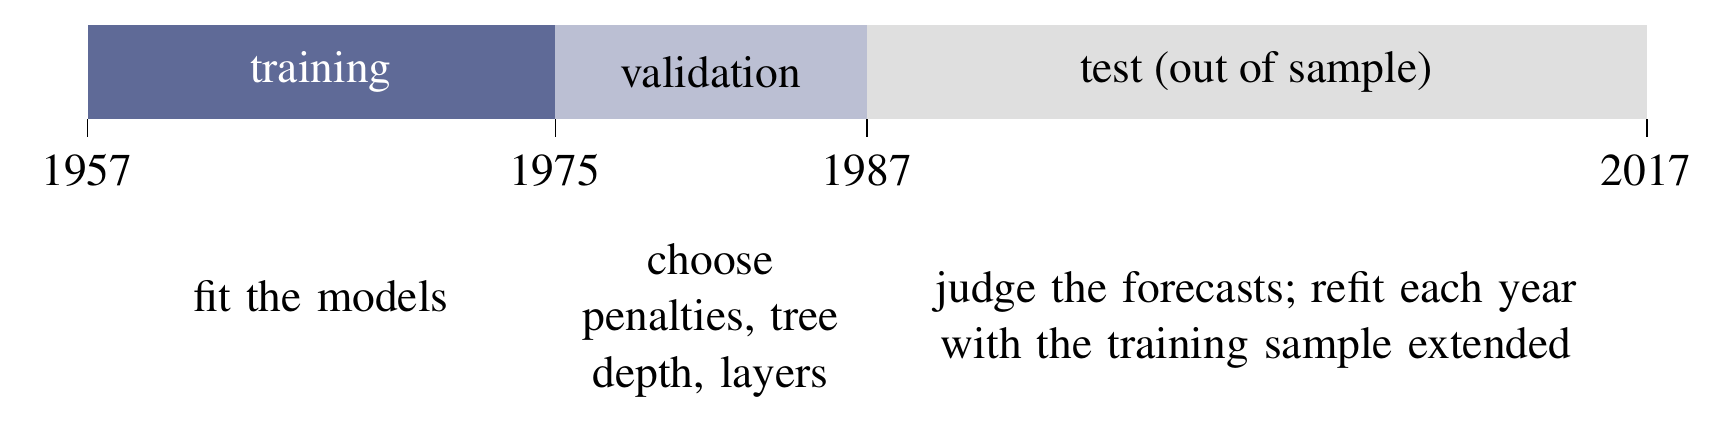
\includegraphics[width=0.9\linewidth]{images/fig21-1-split.png}
\caption{The time split in Gu, Kelly and Xiu (2020). Models are fitted on 1957--1974, their tuning parameters chosen on 1975--1986, and their forecasts judged on 1987--2016, a test period that played no part in fitting or tuning.}
\label{fig:21-split}
\end{figure}

\textbf{Measuring success.} Gu, Kelly and Xiu (2020) use an out-of-sample $R^2$ measured against a forecast of zero:
\begin{equation}
  R^2_{oos} = 1 - \frac{\sum (r_{i,t+1} - \hat{r}_{i,t+1})^2}{\sum r_{i,t+1}^2}
  \label{eq:21-r2}
\end{equation}
For individual stocks, a monthly $R^2$ of a few tenths of a percent is economically large (Figure~\ref{fig:21-gkx}). The \textbf{Diebold--Mariano test} checks whether one model's forecast errors are smaller than another's by more than chance. The economic test is a \textbf{long--short portfolio}: each month, buy the assets with the highest forecasts and sell those with the lowest.

\begin{figure}[htbp]
\centering
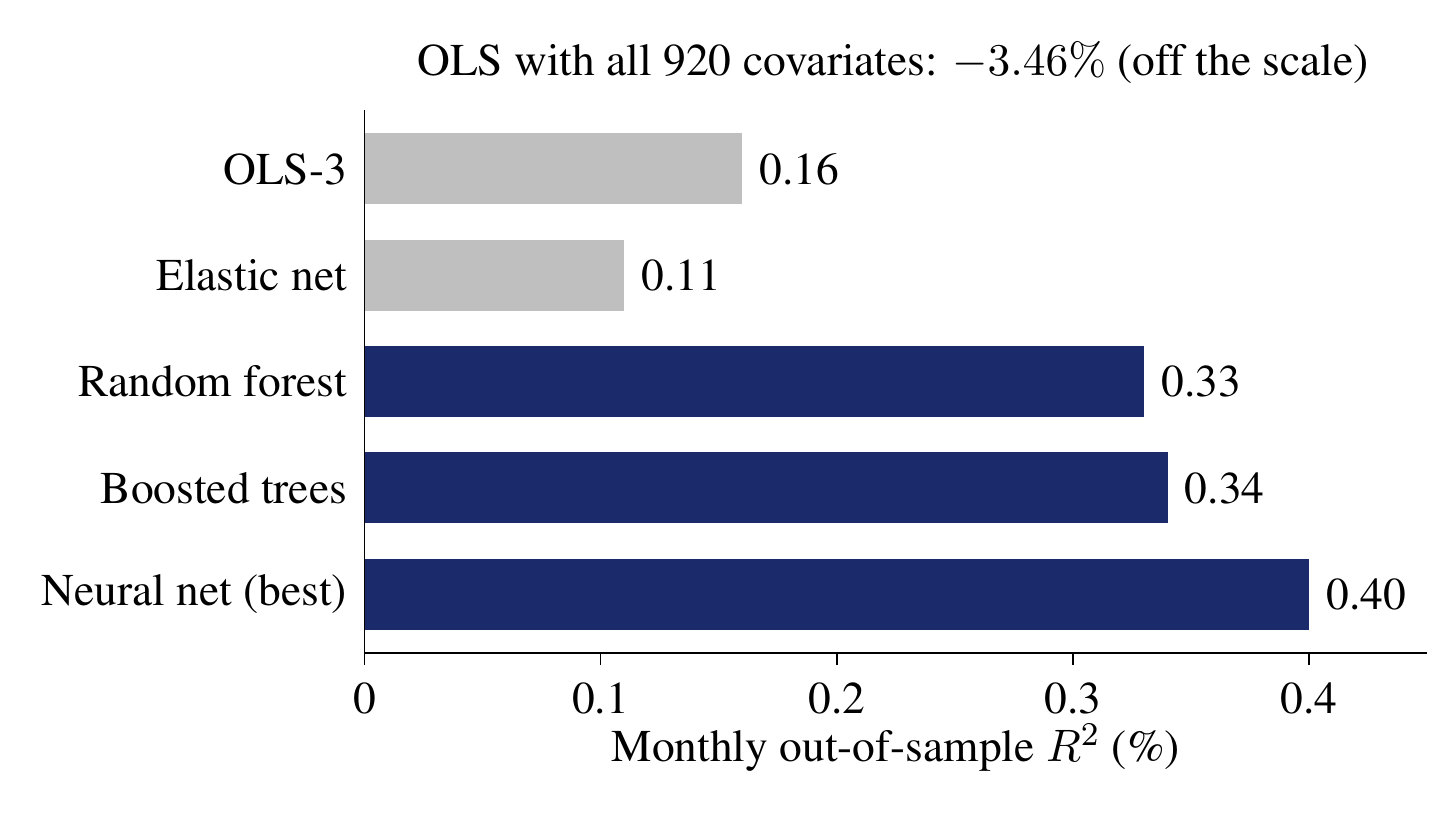
\includegraphics[width=0.85\linewidth]{images/fig21-2-gkx-r2.png}
\caption{Monthly out-of-sample $R^2$ for individual U.S. stocks, 1987--2016, from Gu, Kelly and Xiu (2020). Trees and neural networks roughly doubled the $R^2$ of a three-characteristic OLS model. OLS on all 920 covariates, at $-3.46\%$, was far worse than forecasting zero.}
\label{fig:21-gkx}
\end{figure}

\textbf{Worked example.} A stock's monthly return has a volatility of 10\%. A model that explains 0.4\% of its variance has forecasts with a volatility of $\sqrt{0.004} \times 10\% = 0.63\%$ a month.

\begin{itemize}
  \item If the forecasts are unbiased, the gap in expected return between a stock forecast one standard deviation above average and one forecast one standard deviation below is about 1.3\% a month, or more than 15\% a year.
  \item Applied across thousands of stocks, a tiny $R^2$ can support a profitable strategy.
  \item Most of that spread, however, may come from small, illiquid stocks that are costly to trade.
\end{itemize}

\textbf{Interpreting a model.} \textbf{Permutation importance} shuffles one input at a time, breaking its link to returns, and measures how much the forecast accuracy falls.

\textbf{Complexity.} Classical statistics warns against models with more parameters $P$ than observations $T$. Recent theory on ``benign overfitting'' shows that heavily over-parameterized models with a small ridge penalty can still forecast well out of sample. Kelly, Malamud and Zhou (2024) argued that this applies to return prediction.

\textbf{Further reading.} Hastie, Tibshirani and Friedman, \emph{The Elements of Statistical Learning}, and James, Witten, Hastie and Tibshirani, \emph{An Introduction to Statistical Learning} (regularization, trees, boosting, validation); Goodfellow, Bengio and Courville, \emph{Deep Learning}; Kelly and Xiu, ``Financial Machine Learning'' (\emph{Foundations and Trends in Finance}), and Nagel, \emph{Machine Learning in Asset Pricing}; L\'opez de Prado, \emph{Advances in Financial Machine Learning} (backtest overfitting in practice).

\section{How it works}
\label{sec:21-how}

A machine-learning return model has three ingredients: the inputs, the model and the discipline that keeps it honest.

\textbf{Inputs.} Academic studies use dozens to hundreds of stock characteristics: size, value, momentum, profitability, investment, volatility, liquidity and many accounting ratios. Most come from the anomaly literature of Chapters 8 to 12. Some studies add macroeconomic variables and let the model learn how the value of each characteristic changes with the economy.

\textbf{Model.} Where a linear model adds up characteristics with fixed weights, a tree or neural network can learn that momentum works differently in small and large stocks, or that high volatility hurts returns only beyond a threshold. These are the interactions and nonlinearities that the claim says are hidden.

\textbf{Discipline.} Flexibility is also the danger. A model with enough freedom will fit the noise in any training sample. The defences are:

\begin{itemize}
  \item a strict time split between training, validation and testing;
  \item penalties and early stopping, tuned on validation data only;
  \item averaging over random seeds and many models;
  \item a final test period long enough to separate skill from luck.
\end{itemize}

Three features of finance make the task harder than image recognition:

\begin{itemize}
  \item \textbf{The signal is weak.} Most of a stock's monthly return is unpredictable noise.
  \item \textbf{The data are few.} A century of monthly data is about 1,200 time periods.
  \item \textbf{The target moves.} Once investors learn a pattern, it tends to shrink (Chapter 10).
\end{itemize}

Finally, a forecast is only as valuable as the portfolio built from it. If the predictability lives in small, illiquid stocks, or requires trading half the portfolio each month, little of it reaches an investor.

\section{The claim}
\label{sec:21-claim}

\begin{callout}
\textbf{Claim.} Machine-learning models find return predictability that traditional linear models miss, and it can be turned into profitable portfolios.
\end{callout}

The claim has three parts, each of which can fail on its own:

\begin{itemize}
  \item \textbf{Statistical:} flexible models forecast returns out of sample better than linear models using the same inputs.
  \item \textbf{Hidden:} the gain comes from interactions or nonlinear effects, not from simply using more of the characteristics already known to predict returns.
  \item \textbf{Economic:} the gain survives trading costs and holds among stocks large enough to trade.
\end{itemize}

\section{The original evidence}
\label{sec:21-evidence}

\textbf{Gu, Kelly and Xiu (2020).} The landmark study used monthly CRSP returns for almost 30,000 U.S. stocks from March 1957 to December 2016, an average of more than 6,200 a month. Inputs were 94 stock characteristics, 8 macroeconomic predictors and 74 industry dummies, about 920 covariates once characteristics were interacted with macro variables. Models were trained on 1957--1974, validated on 1975--1986 and tested on 1987--2016.

\begin{center}
\small
\begin{tabularx}{0.9\linewidth}{@{}>{\raggedright\arraybackslash}X>{\raggedright\arraybackslash}p{0.35\linewidth}@{}}
\toprule
Model & Monthly out-of-sample $R^2$ (\%) \\
\midrule
OLS, all covariates & $-3.46$ \\
OLS-3 (size, book-to-market, momentum) & 0.16 \\
Elastic net & 0.11 \\
Random forest & 0.33 \\
Gradient-boosted trees & 0.34 \\
Neural networks (one to five layers) & 0.33 to 0.40 \\
\bottomrule
\end{tabularx}
\end{center}

A long--short decile portfolio sorted on neural-network forecasts earned an annualized Sharpe ratio of 1.35 value-weighted and 2.45 equal-weighted. The corresponding figures for the benchmark OLS model were 0.61 and 0.83. All methods agreed on the dominant signals: price trends (momentum, industry momentum, short-term reversal), liquidity (size, dollar volume, bid--ask spread) and volatility (total and idiosyncratic volatility, beta).

Two details matter for what follows. OLS with all covariates was a disaster, so regularization of some kind is essential. And the gap between equal-weighted and value-weighted results suggests that much of the profit comes from small stocks.

\textbf{Avramov, Cheng and Metzker (2023).} Avramov, Cheng and Metzker examined where machine-learning profits come from. Excluding microcaps, distressed stocks or periods of high market volatility considerably weakened profitability. Reasonable trading costs reduced it further, because the strategies had high turnover and took extreme positions.

\textbf{Kelly, Malamud and Zhou (2024).} Kelly, Malamud and Zhou proved that, in their framework, simple models with few parameters severely understate return predictability compared with complex models that have more parameters than observations. Empirically, they forecast the U.S. stock market with ridge regressions on thousands of random nonlinear transformations of standard market predictors, trained on as little as 12 months of data. They concluded that complexity is a virtue and that machine learning is justified for modelling expected returns.

\textbf{Nagel (2025).} Stefan Nagel showed that when the number of random features greatly exceeds a 12-month training window, the forecast becomes a weighted average of the training-window returns. The weights reflect how similar each past month's predictors are to today's, and in short windows that mostly means how recent the month is. The complex model therefore behaves like a volatility-timed momentum strategy. In artificial data with reversals instead of momentum, the same method still builds that strategy and does poorly. On this reading, the virtue of complexity is a strategy that happened to work, not new information extracted by the model.

The evidence supports the statistical part of the claim, at least for broad stock samples. It is weaker on the hidden part, because the models lean on well-known signals. It is weakest on the economic part.

\section{Replication lab: machine learning on a portfolio panel}
\label{sec:21-lab}

\begin{callout}
\textbf{Lab 21 at a glance.} \emph{Claim on trial:} machine learning finds return predictability that linear models miss, and it survives costs. \emph{Data:} a panel of 149 value-weighted portfolios from the Kenneth R. French Data Library (100 sorted on size and book-to-market, and 49 industries), with the Fama--French factors; the Goyal--Welch predictors for Part D. All are free. \emph{Code:} runs as a script (\texttt{python lab21.py}, or \texttt{python lab21.py -{}-fast}) or as a notebook (\texttt{lab21\_walkthrough.ipynb}) with a prediction prompt before each step.
\end{callout}

Lab 21 cannot use individual stocks, because CRSP is not free. Portfolios average away much of the noise in single stocks and leave out microcaps. The test is therefore closer to what a large investor can trade, but it is not the same test as Gu, Kelly and Xiu's.

Each month the lab computes ten characteristics for every portfolio, ranks them across portfolios and scales them to $[-1, 1]$:

\begin{itemize}
  \item average firm size, number of firms and book-to-market;
  \item last month's return, momentum and long-term reversal;
  \item volatility, beta, idiosyncratic volatility and the largest recent monthly return.
\end{itemize}

Two market variables, the market's past 12-month return and volatility, let the models change their view with conditions. The target is next month's return relative to the average portfolio that month, so the models compete on ranking, not on timing the market.

Five models compete:

\begin{itemize}
  \item OLS on size, value and momentum (OLS-3);
  \item OLS on all twelve inputs;
  \item elastic net;
  \item gradient-boosted trees;
  \item a three-layer neural network averaged over three random seeds.
\end{itemize}

Models are retrained every five years on all earlier data. Their tuning parameters are chosen on the preceding ten years, and the out-of-sample period starts in 1975.

The lab has four parts:

\begin{itemize}
  \item \textbf{Part A} compares out-of-sample $R^2$, Diebold--Mariano tests against OLS-3, and long--short portfolios that buy the top 10\% and sell the bottom 10\% of portfolios by forecast (Figures 21.3 and 21.4).
  \item \textbf{Part B} repeats the comparison for large portfolios only, for 1975--1999 and 2000 onward, and net of trading costs of 10, 25 and 50 basis points per unit of turnover (Figure 21.5).
  \item \textbf{Part C} reruns the network with one seed at a time and measures permutation importance on 2000 onward for models fitted before 2000 (Figure 21.6).
  \item \textbf{Part D} tests the virtue of complexity: ridge regressions on 2 to 1,200 random Fourier features of the Goyal--Welch predictors, with a 12-month rolling window, forecasting the market (Figure 21.7).
\end{itemize}

The command \texttt{python lab21.py -{}-source sim} tests the code on simulated data.

\textbf{What the simulated run shows.} The lab was run end to end only on simulated data. In the simulation, expected returns depend linearly on value and momentum, and nonlinearly on an interaction of size with momentum and on a volatility threshold. A flexible model should therefore win, and the results check that the code can detect a signal of that kind.

\begin{itemize}
  \item Out-of-sample $R^2$ was 0.14\% for OLS-3, 0.19\% for OLS on all inputs, 0.18\% for the elastic net, 0.21\% for gradient-boosted trees and 0.19\% for the network. Only the trees beat OLS-3 decisively (Diebold--Mariano $t = 3.6$). OLS on all inputs and the network managed $t = 2.0$.
  \item Before costs, long--short Sharpe ratios ranged from 1.12 (OLS-3) to 1.32 (trees). The trees also traded most.
  \item Among large portfolios, the trees kept a Sharpe ratio of 1.09 against 0.76 to 0.80 for the other models.
  \item At 25 bp per unit of turnover, OLS on all inputs had the highest Sharpe ratio (0.83), ahead of the trees (0.77). At 50 bp, the trees fell to 0.22 and OLS on all inputs held 0.43.
  \item With a single seed, the network's $R^2$ ranged from 0.16\% to 0.18\% and its Sharpe ratio from 1.17 to 1.32.
  \item All three models ranked momentum as the most important input; the trees also leaned on volatility, as the simulation intended.
  \item In Part D, where the simulated predictors carried almost no information, models with as many features as observations and a tiny ridge penalty produced an $R^2$ of about $-1{,}200\%$. With heavy shrinkage, $R^2$ stayed near zero at every level of complexity.
\end{itemize}

On real data the lab answers what the simulation cannot: whether real portfolios contain nonlinear structure that the flexible models find, and whether it survives costs.

\section{Stress tests}
\label{sec:21-stress}

\textbf{The universe.} The single biggest influence on machine-learning results is which assets are included. Gu, Kelly and Xiu's equal-weighted Sharpe ratio was almost twice the value-weighted one. Avramov, Cheng and Metzker found that removing microcaps and distressed firms considerably weakened profits. The lab's portfolio panel removes microcaps by construction and adds a large-portfolio subset.

\textbf{Trading costs.} Flexible models tend to trade more, because small changes in inputs can flip a forecast. In the simulated run, the model with the best gross Sharpe ratio fell behind a linear model at 25 bp per unit of turnover. Costs should be charged at the level the investor actually pays, and turnover reported alongside every Sharpe ratio (Chapter 6).

\textbf{Time.} Results from 1987--2016 include the years before many anomalies were published and arbitraged (Chapter 10). The lab splits the out-of-sample period at 2000.

\textbf{Tuning and seeds.} Neural networks depend on random initialization and on many choices: layers, penalties, learning rates and stopping rules. A result that holds for one seed or one configuration, but not for others, is closer to luck than to skill. Ensembling over seeds, as Gu, Kelly and Xiu did, helps, and the lab reports single-seed results to show the spread.

\textbf{Researcher degrees of freedom.} Every published model is the survivor of many tried. The tuning sample controls overfitting within one design, but not the choice among designs (Chapter 4).

\textbf{Complexity in timing.} Kelly, Malamud and Zhou's result depends on the window, the penalty and the predictors. Nagel's reinterpretation implies a sharp test: if the complex model's timing signal is close to a simple volatility-scaled momentum rule, the complexity adds little. Exercise 8 runs that comparison.

\section{Verdict}
\label{sec:21-verdict}

\begin{callout}
\textbf{Verdict: weakens} (as of October 2026). The statistical part of the claim holds. In broad samples of U.S. stocks, regularized nonlinear models forecast returns out of sample better than linear models with a few characteristics, and the improvement is too large and consistent to be luck (Gu, Kelly and Xiu 2020). The other two parts are much weaker.
\end{callout}

\begin{itemize}
  \item \textbf{Not very hidden.} The models rely mostly on signals already known (momentum, short-term reversal, size, liquidity and volatility). Much of the gain comes from combining many such signals with appropriate shrinkage, which a well-regularized linear model also captures in part.
  \item \textbf{Not easily captured.} The economic gains are concentrated in small and distressed stocks and in volatile periods, and they shrink after realistic trading costs (Avramov, Cheng and Metzker 2023). The gap between equal-weighted and value-weighted results points the same way.
  \item \textbf{Complexity disputed.} The virtue of complexity in market timing may be a volatility-timed momentum strategy in disguise (Nagel 2025).
\end{itemize}

Machine learning is a better tool for an old job, not a source of hidden alpha. The verdict would move to \emph{survives} if value-weighted, net-of-cost machine-learning portfolios beat regularized linear ones among large stocks, out of sample after 2016, by a significant margin.

\section{What investors can use}
\label{sec:21-investors}

\begin{itemize}
  \item \textbf{Machine learning is a better blender, not a crystal ball.} Its proven value is in combining many known signals with care about overfitting. Expect modest improvements over a well-built linear multi-factor model, not a new source of returns.
  \item \textbf{Ask where the returns come from.} A strategy whose edge sits in microcaps, in the short side or in months of market stress may not be available at scale or after costs.
  \item \textbf{Insist on the net, value-weighted number.} Equal-weighted, gross-of-cost backtests flatter flexible models most.
  \item \textbf{Treat interpretability as a risk control.} If a manager cannot say which signals drive the forecasts, it is impossible to judge whether they will persist.
  \item \textbf{Expect decay.} Signals published in the academic literature lose part of their power after publication (Chapter 10). A model trained on them inherits the decay.
\end{itemize}

\textbf{Questions to ask a manager who sells machine-learning strategies:}

\begin{itemize}
  \item What is the out-of-sample period, and how often were the model and its tuning changed during it?
  \item How do results compare with a linear model on the same inputs, net of costs and value-weighted?
  \item How much of the return comes from the 20\% smallest stocks, and from the short side?
  \item What is the monthly turnover, and what trading costs are assumed?
  \item How much do results change with the random seed or with small changes to the training window?
\end{itemize}

\begin{callout}
\textbf{What Failed: the AI fund that trailed the index.} In 2017 the AI Powered Equity ETF (ticker AIEQ) launched as the first exchange-traded fund run by artificial intelligence. Its manager, EquBot, used IBM Watson to process news, filings and market data and to monitor tens of thousands of models. By January 2022 the fund was up 57\% since inception, while the S\&P 500 total return index was up 84\% over the same period (Tech Brew 2022). Assets were about \$150 million. The models were sophisticated; the difficulty was the task. Stock returns carry little signal, the competition for it is intense, and a model that learns from the past is always learning about a market that has already moved on.
\end{callout}

\section{Open questions}
\label{sec:21-open}

\begin{itemize}
  \item \textbf{Does the edge survive among large stocks?} The strongest machine-learning results come from broad samples dominated by small stocks. How much remains in the largest 500 or 1,000?
  \item \textbf{Hidden or known?} Do flexible models find genuinely new interactions, or mostly better ways to combine momentum, volatility and liquidity?
  \item \textbf{Complexity or momentum?} Is the virtue of complexity in market timing a general result or, as Nagel argues, a disguised volatility-timed momentum strategy?
  \item \textbf{New models and new data.} Chapter 22 asks the parallel question for time-series foundation models, and Chapter 23 for language models applied to news.
\end{itemize}

\section*{Exercises}
\addcontentsline{toc}{section}{Exercises}

\subsection*{Conceptual (all readers)}

\begin{enumerate}
  \item A model has a monthly out-of-sample $R^2$ of 0.3\% on stocks with 12\% monthly volatility. What is the standard deviation of its forecasts? What expected return gap separates stocks forecast one standard deviation above and below average?
  \item Explain why OLS with 920 covariates had an out-of-sample $R^2$ of $-3.46\%$ in Gu, Kelly and Xiu (2020), while OLS with three characteristics had $+0.16\%$.
  \item A gradient-boosted model uses trees of depth 1. Can it capture an interaction between size and momentum? What about depth 2?
\end{enumerate}

\subsection*{Lab extensions (technical readers)}

\begin{enumerate}
  \setcounter{enumi}{3}
  \item Part A: run on real data. Is the Diebold--Mariano statistic of the best nonlinear model against OLS-3 above 2?
  \item Compare the long--short Sharpe ratio of each model on all portfolios and on large portfolios only. Which model loses most?
  \item At what cost per unit of turnover does the best model's long--short Sharpe ratio fall below that of OLS-3?
  \item Part C: rank the characteristics by importance for the trees and for OLS. Do the flexible models rely on anything the linear model ignores?
  \item Part D: compute a volatility-scaled momentum rule for the market (last 12 months' return divided by trailing volatility) and correlate its timing signal with the complex model's forecasts. How much of the complex model's performance does the simple rule reproduce?
  \item Gu, Kelly and Xiu report much higher Sharpe ratios for equal-weighted than for value-weighted portfolios. What does that suggest about where the predictability lives, and about whether investors can capture it?
  \item A start-up claims its deep-learning model earned a Sharpe ratio of 3 in a backtest over 2010--2024. List the questions you would ask before investing.
\end{enumerate}

\section*{References}
\addcontentsline{toc}{section}{References}

\begin{itemize}
  \item Avramov, D., Cheng, S. and Metzker, L. (2023). Machine Learning vs.\ Economic Restrictions: Evidence from Stock Return Predictability. \emph{Management Science} 69(5): 2587--2619.
  \item Gu, S., Kelly, B. and Xiu, D. (2020). Empirical Asset Pricing via Machine Learning. \emph{Review of Financial Studies} 33(5): 2223--2273.
  \item Kelly, B., Malamud, S. and Zhou, K. (2024). The Virtue of Complexity in Return Prediction. \emph{Journal of Finance} 79(1): 459--503.
  \item Nagel, S. (2025). Seemingly Virtuous Complexity in Return Prediction. NBER Working Paper 34104.
  \item Tech Brew (2022). How the World's First AI-Managed ETF Stacks Up Almost Five Years Later. January 26.
\end{itemize}

\textbf{Data:} Kenneth R. French Data Library: 100 Portfolios Formed on Size and Book-to-Market (10 $\times$ 10); 49 Industry Portfolios; Fama/French 3 Factors. Goyal--Welch predictor data (Amit Goyal's website), for Part D.

% Chapter 22 -- Claim: Foundation Models Beat Classical Forecasts
% Requires: amsmath, amssymb, booktabs, array, tabularx, graphicx, tcolorbox (breakable, skins), hyperref or url.
% Defines the callout box only if the preamble has not.
\providecolor{fenavy}{HTML}{1B2A6B}
\providecolor{feshade}{HTML}{F3F5FA}
\makeatletter
\@ifundefined{callout}{%
  \newtcolorbox{callout}{breakable, enhanced,
    colback=white, colframe=gray!70, boxrule=0.5pt, arc=1mm,
    borderline west={2.5pt}{0pt}{gray!70},
    left=8pt, right=8pt, top=4pt, bottom=4pt}%
}{}
\makeatother

\chapter{Claim: Foundation Models Beat Classical Forecasts}
\label{ch:22}

Large language models learned to write by reading most of the internet. Since 2024, the same recipe has been applied to numbers. Time-series foundation models, such as Amazon's Chronos and Google's TimesFM, are pretrained on billions of observations from thousands of series: electricity demand, web traffic, weather, retail sales. They then forecast series they have never seen, with no training at all. Their developers report that, used this way, they match or beat models fitted specifically to each dataset.

For finance and economics the promise is striking: one pretrained model, applied to returns, volatility or inflation, could replace the careful work of specifying and estimating a model for each series.

Financial series are unlike most of the data these models learn from. Returns are close to unpredictable, volatility has long memory and fat tails, and macroeconomic series are short and revised. Public financial data may also have been part of the training set, which can flatter a model on history. This chapter asks whether foundation models beat simple classical benchmarks once those problems are taken seriously.

By the end of the chapter you will be able to:

\begin{itemize}
  \item name the classical benchmark for each kind of series: the historical mean, the naive forecast, autoregressions, GARCH and HAR;
  \item explain how a time-series foundation model is pretrained and used zero-shot, and how Chronos and TimesFM differ;
  \item explain contamination, and why only data published after a model's training cutoff give a clean test;
  \item evaluate forecasts on rolling origins with MSE ratios, the Diebold--Mariano test, interval coverage and the pinball and QLIKE losses;
  \item calculate how long an evaluation sample must be to detect a small gain;
  \item state the claim and judge the evidence on returns, volatility, other financial series and macroeconomic series.
\end{itemize}

\section{Foundations: benchmarks, foundation models and fair tests}
\label{sec:22-foundations}

\textbf{Classical benchmarks.} A forecasting method earns attention only if it beats simple alternatives:

\begin{itemize}
  \item The \textbf{historical mean} forecasts the average of all past values. It is hard to beat for stock returns (Chapter 7).
  \item The \textbf{naive} or random-walk forecast is the last observed value. It is hard to beat for exchange rates and interest-rate levels.
  \item An \textbf{autoregression}, AR($p$), regresses the series on its own past $p$ values:
  \begin{equation}
    y_{t+1} = c + \phi_1 y_t + \cdots + \phi_p y_{t-p+1} + \varepsilon_{t+1}
    \label{eq:22-ar}
  \end{equation}
  The number of lags can be chosen by an information criterion such as BIC. \textbf{ARIMA} models add differencing and moving-average terms.
  \item For volatility, \textbf{GARCH} models update the variance with each squared return (Chapter 11), and the \textbf{HAR} model regresses realized variance on its recent daily, weekly and monthly averages (Corsi 2009). Both capture volatility's long memory with few parameters.
\end{itemize}

\textbf{Foundation models.} A time-series foundation model is a large neural network, usually a \textbf{transformer}, pretrained on a broad collection of series and then used \textbf{zero-shot}, without any training on the target series. Two design families matter here:

\begin{itemize}
  \item \textbf{Chronos} (Ansari et al.\ 2024) scales each series and quantizes its values into a fixed vocabulary of tokens. It then trains a T5 language-model architecture to predict the next token, which yields a full probability distribution for the forecast. Models range from 20 million to 710 million parameters. Chronos-Bolt is a faster successor.
  \item \textbf{TimesFM} (Das et al.\ 2024) is a decoder-only transformer of about 200 million parameters. It reads the series in patches of consecutive points and outputs longer patches. It was pretrained on about 100 billion time points, mostly Google Trends search interest and Wikipedia page views, plus synthetic series.
\end{itemize}

The pitch is breadth: a model that has seen trends, seasonality, mean reversion and regime shifts across many domains should recognize them in a new series.

\textbf{Contamination.} A forecast evaluation is valid only if the model has not seen the test data. Classical models are fitted on past data at each forecast date, so this is easy to guarantee. A foundation model's pretraining corpus is fixed and often only partly documented. If it contains the test series, or close copies such as a stock index that tracks the target, the model may partly be remembering rather than forecasting. The clean test uses data published after the model's \textbf{training cutoff}.

\textbf{Evaluation.} Forecasts are compared on the same \textbf{rolling origins}: at each month $t$, every model forecasts month $t+1$ using only data up to $t$ (Figure~\ref{fig:22-rolling}).

\begin{itemize}
  \item The \textbf{mean squared error (MSE) ratio} divides a model's MSE by that of a benchmark; below 1 means better.
  \item The \textbf{Diebold--Mariano test} (Diebold and Mariano 1995) checks whether the average difference in squared errors is significantly different from zero.
  \item For distributional forecasts, \textbf{coverage} asks whether an 80\% interval contains the outcome 80\% of the time, and the \textbf{pinball loss} scores each quantile.
  \item For volatility, the \textbf{QLIKE} loss is robust to noise in the realized-variance proxy (Patton 2011; Section~\ref{sec:11-eval}).
\end{itemize}

\begin{figure}[htbp]
\centering
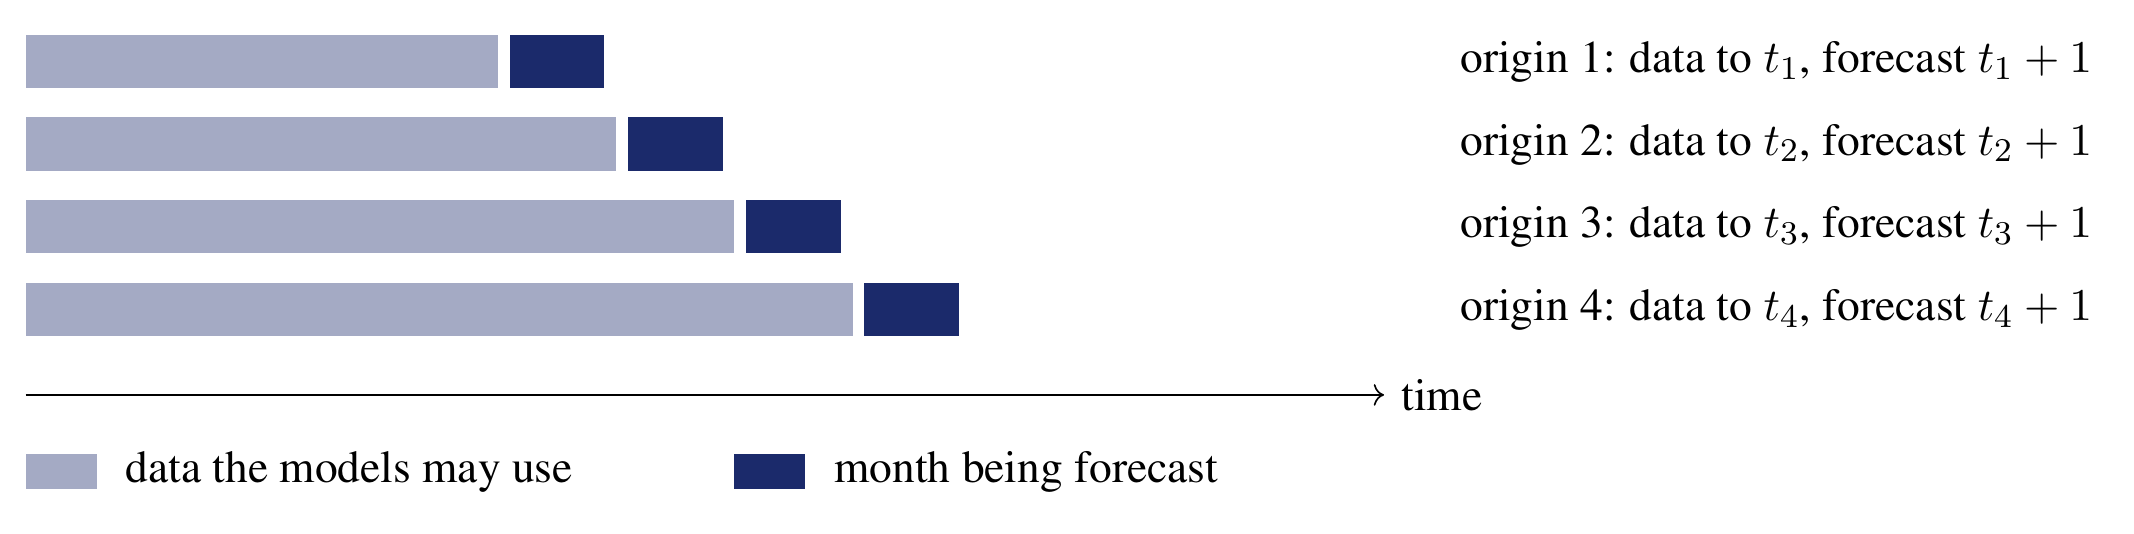
\includegraphics[width=0.85\linewidth]{images/fig22-1-rolling.png}
\caption{Rolling-origin evaluation. At each origin every model sees the same data up to that month and forecasts the next one; the origin then moves forward a month. No model ever sees the month it is forecasting.}
\label{fig:22-rolling}
\end{figure}

\textbf{Worked example.} Suppose an AR model's one-month inflation forecasts have an MSE of 0.040 (percentage points squared) over 300 months and a foundation model's 0.038.

\begin{itemize}
  \item The MSE ratio is 0.95, a 5\% gain.
  \item If the monthly loss differences have a standard deviation of 0.020 and little autocorrelation, the Diebold--Mariano statistic is $0.002 / (0.020/\sqrt{300}) \approx 1.7$, not significant at 5\%.
  \item A gain of that size needs a long evaluation sample to be distinguished from luck, and a post-cutoff window of two years has only 24 observations (Figure~\ref{fig:22-dm}).
\end{itemize}

\begin{figure}[htbp]
\centering
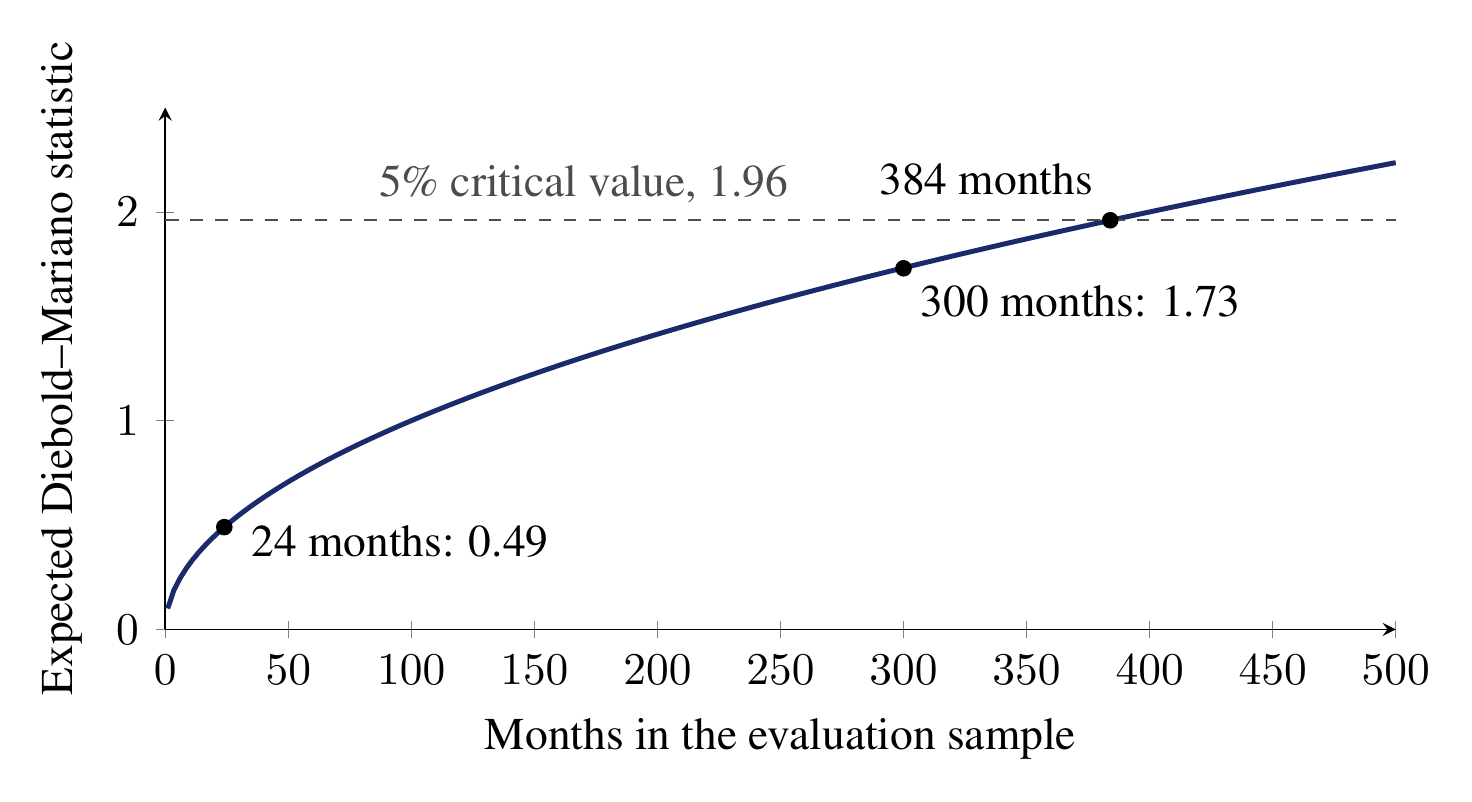
\includegraphics[width=0.85\linewidth]{images/fig22-2-dm-power.png}
\caption{The expected Diebold--Mariano statistic for the worked example's 5\% gain, as the evaluation sample grows. It reaches 1.96 only after about 384 months; a two-year post-cutoff window gives about 0.5.}
\label{fig:22-dm}
\end{figure}

\textbf{Further reading.} Hyndman and Athanasopoulos, \emph{Forecasting: Principles and Practice}, and Diebold, \emph{Elements of Forecasting} (forecasting principles and classical methods); Hamilton, \emph{Time Series Analysis}, and Tsay, \emph{Analysis of Financial Time Series}; Elliott and Timmermann, \emph{Economic Forecasting} (forecast evaluation); Goodfellow, Bengio and Courville, \emph{Deep Learning} (transformers and pretraining).

\section{How it works}
\label{sec:22-how}

A zero-shot forecast takes three steps. The recent history of a series, up to a few hundred observations, is normalized and passed to the pretrained network. The network outputs a forecast for the next step or steps, often as a set of quantiles. Nothing is estimated on the target series; all the knowledge comes from pretraining.

That design has clear strengths:

\begin{itemize}
  \item \textbf{No specification work.} There are no lags to choose and no model to estimate.
  \item \textbf{Short histories.} Patterns learned elsewhere can fill in for a lack of data on the target series.
  \item \textbf{Probabilistic output.} Forecast intervals come built in.
\end{itemize}

It also has limits that bite hardest in finance:

\begin{itemize}
  \item \textbf{Weak signal.} Most of the variation in a monthly return is noise. A model trained to extend patterns may find them where none exist.
  \item \textbf{Domain mismatch.} Pretraining corpora are dominated by series with strong seasonality and trends: energy demand, traffic, sales. Financial returns have neither, and volatility has dynamics that few other series share.
  \item \textbf{Scale and context.} Normalizing each window discards the level of a series. For volatility or inflation, the level itself carries information about what comes next.
  \item \textbf{Contamination.} Popular financial and macroeconomic series are widely published, so a model may have seen them, or close relatives, in pretraining.
\end{itemize}

Classical models are the opposite: narrow, but fitted to the target series and transparent about what they assume. The question is whether breadth beats fit.

\section{The claim}
\label{sec:22-claim}

\begin{callout}
\textbf{Claim.} Pretrained time-series foundation models, used zero-shot, forecast financial and economic series better than classical models.
\end{callout}

To count as evidence, a test must:

\begin{itemize}
  \item compare against strong classical benchmarks for each series (the historical mean for returns, AR models for macroeconomic series, HAR for realized volatility), not only against naive forecasts;
  \item use rolling origins, with each forecast made only from data available at the time;
  \item report significance, not just average losses;
  \item show that the result holds on data the model cannot have seen during pretraining.
\end{itemize}

\section{The original evidence}
\label{sec:22-evidence}

\textbf{The developers' benchmarks.}

\begin{itemize}
  \item \textbf{Chronos (Ansari et al.\ 2024).} Chronos was pretrained on a large collection of public datasets plus synthetic series generated from Gaussian processes, and evaluated on 42 datasets. On datasets that were part of its training corpus, it significantly outperformed other methods. On new datasets, its zero-shot performance was comparable to, and occasionally better than, models trained on those datasets.
  \item \textbf{TimesFM (Das et al.\ 2024).} Google reported that TimesFM beat statistical methods such as ARIMA and ETS on unseen data, and matched or beat deep-learning models trained on the target series, on standard benchmark archives.
\end{itemize}

These benchmarks contain few financial series. The Chronos result also illustrates the contamination problem: performance was strongest on data the model had seen.

\textbf{Daily stock returns (Rahimikia, Ni and Wang 2025).} Rahimikia, Ni and Wang tested Chronos, TimesFM and other foundation models on daily excess returns of securities in 94 countries from 1990 to 2023, out of sample from 2001. Off-the-shelf models performed poorly. Zero-shot Chronos (large) had an out-of-sample $R^2$ of $-1.37\%$, with about 51\% directional accuracy, and TimesFM had $-2.80\%$. Fine-tuning helped little. Pretraining the same architectures from scratch on financial data improved them substantially, but they still trailed tree ensembles such as CatBoost on $R^2$. The authors concluded that generic pretraining does not transfer directly to finance.

\textbf{Multivariate financial series (Marconi 2025).} Marconi evaluated Tiny Time Mixers and Chronos on changes in the U.S. 10-year Treasury yield, EUR/USD volatility and an equity spread. Zero-shot, the models beat naive baselines on volatility and the spread. Fine-tuning a pretrained model beat training the same architecture from scratch, and needed several fewer years of data. But specialised traditional models matched or beat the foundation model on two of the three tasks.

\textbf{Realized volatility (Brini 2026).} Brini compared nine zero-shot foundation models with eight econometric models, including HAR variants and ARFIMA. The data were daily realized volatility for 40 U.S. stocks, five currency pairs and five futures contracts, at horizons of 1, 5 and 22 days. Pooled losses favoured the foundation models, but the advantage came from a few outlier assets. On average per-asset QLIKE loss, only one model (Tiny Time Mixers) beat a log-HAR benchmark at every horizon, by about 1.3\% to 1.8\%; the other eight did not. An equal-weight average of that model and log-HAR was among the best forecasts for almost every asset.

The pattern across studies is consistent. Zero-shot foundation models beat naive forecasts easily, sometimes match well-specified classical models, and rarely beat them by a meaningful margin. Where they do, combining them with a classical model helps more than replacing it.

\section{Replication lab: six series, one month ahead}
\label{sec:22-lab}

\begin{callout}
\textbf{Lab 22 at a glance.} \emph{Claim on trial:} foundation models, used zero-shot, beat classical forecasts. \emph{Data:} the U.S. market's excess return and its log realized variance built from daily returns (Kenneth R. French Data Library); inflation, industrial production growth, and the changes in the unemployment rate and in the 10-year Treasury yield (FRED). All are free. \emph{Code:} runs as a script (\texttt{python lab22.py -{}-models chronos-bolt-small timesfm}) or as a notebook (\texttt{lab22\_walkthrough.ipynb}) with a prediction prompt before each step.
\end{callout}

Lab 22 forecasts the six series one month ahead, from every month since January 2000. At each month, every model sees only data up to that month.

\begin{center}
\small
\begin{tabularx}{0.9\linewidth}{@{}>{\raggedright\arraybackslash}X>{\raggedright\arraybackslash}p{0.38\linewidth}@{}}
\toprule
Model & Type \\
\midrule
Historical mean & Classical \\
Naive (last value) & Classical \\
AR, lags chosen by BIC on the last 30 years & Classical: \textbf{the benchmark} \\
HAR-type: last value, 3-month and 12-month averages & Classical \\
GARCH(1,1), realized variance only & Classical \\
Chronos-Bolt (small and base) & Foundation model, zero-shot \\
TimesFM & Foundation model, zero-shot \\
\bottomrule
\end{tabularx}
\end{center}

The foundation models are optional, because they need PyTorch and large model downloads (\texttt{pip install chronos-forecasting timesfm}). Without them, the lab runs everything else and reports which models could not be loaded.

The lab has four parts:

\begin{itemize}
  \item \textbf{Part A} reports each model's MSE relative to AR, and its $R^2$ against the historical mean (Figures 22.3 and 22.7).
  \item \textbf{Part B} adds Diebold--Mariano tests, the share of months each model beats AR and the cumulative squared-error difference over time (Figure 22.4).
  \item \textbf{Part C} splits the evaluation at a cutoff date, by default January 2024, to be set to each model's training cutoff. A deliberately contaminated ``memorizing'' model, which is shown the answer before the cutoff, displays the signature of contamination (Figure 22.5).
  \item \textbf{Part D} checks whether each model's 80\% forecast intervals contain the outcome 80\% of the time (Figure 22.6).
\end{itemize}

The command \texttt{python lab22.py -{}-source sim -{}-models standin} tests the code.

\textbf{What the simulated run shows.} The lab was run end to end only on simulated data, and without any foundation model. A clearly labelled stand-in, the average of three classical forecasts, took the foundation models' place. The results test the code and illustrate the evaluation, not the models.

\begin{itemize}
  \item For simulated returns, which are unpredictable by construction, the historical mean beat AR (MSE ratio 0.98) and the naive forecast doubled the error (1.99).
  \item For simulated log realized variance, which has long memory, HAR and AR were nearly tied (0.996), the historical mean was nine times worse, and GARCH on monthly returns was almost three times worse. GARCH sees only one return a month, while the realized-variance models see daily data.
  \item The stand-in never beat AR significantly; it was worse on five of six series, by up to 12\%.
  \item The memorizing model had an MSE ratio of 0.16 before the cutoff and exactly 1.00 after it. That collapse is what contamination looks like.
  \item The AR and HAR-type models' 80\% intervals contained the outcome 79\% to 81\% of the time; the historical mean's interval for realized variance managed only 53\%.
\end{itemize}

Run with the foundation models on real data, the lab answers the chapter's question directly: whether they beat AR and HAR, whether their edge survives the cutoff and whether their intervals are honest.

\section{Stress tests}
\label{sec:22-stress}

\textbf{Benchmark strength.} Most claims of superiority are made against naive forecasts or against classical models that were not tuned for the target series. Against the historical mean for returns, AR for macroeconomic series and HAR for volatility, the gap narrows or disappears.

\textbf{Contamination.} The only clean evaluation is on data published after the model's training cutoff. Developers rarely list every series in their corpora, so cutoff dates are often approximate. A post-cutoff window of a year or two is short for monthly data, and significance tests will have little power.

\textbf{Frequency and horizon.} Studies of daily realized volatility at horizons of 1 to 22 days find small, uneven gains. Monthly series give far fewer observations. Gains may appear at some horizons and not others, so results should be reported by horizon.

\textbf{Pooled versus per-series results.} A model can win on pooled losses because of a few series with large errors while losing on most series. Brini's realized-volatility study found exactly that. Per-series results, or losses scaled to each series, avoid the problem.

\textbf{Model versions.} Foundation models are updated often, and results for one version may not hold for the next. Evaluations should name the exact model and version.

\textbf{Context length.} Foundation models normalize each input window. Giving them 64 rather than 512 months of history can change both the forecast and its interval.

\section{Verdict}
\label{sec:22-verdict}

\begin{callout}
\textbf{Verdict: provisional} (as of October 2026). The evidence so far does not support the claim, but it is too new and too thin to reject it.
\end{callout}

\begin{itemize}
  \item \textbf{Returns.} Zero-shot foundation models forecast stock returns worse than simple benchmarks (Rahimikia, Ni and Wang 2025). Pretraining on financial data helps, which suggests the problem is the domain, not the architecture.
  \item \textbf{Volatility.} Most foundation models do not beat a well-specified HAR model on average. The best one beats it by one or two percent, and the most reliable forecast combines the two (Brini 2026).
  \item \textbf{Other financial series.} Foundation models beat naive baselines but are matched or beaten by specialised models in most tasks studied (Marconi 2025).
  \item \textbf{Macroeconomic series.} Clean, post-cutoff evaluations are still scarce.
\end{itemize}

The field changes quickly, and models pretrained on financial data are appearing. The verdict should be revisited when there are post-cutoff evaluations of several years for the main financial and macroeconomic series. It would move to \emph{survives} if a foundation model beat AR and HAR significantly on data it cannot have seen, and to \emph{fails} if successive generations continued to fall short of them.

\section{What investors can use}
\label{sec:22-investors}

\begin{itemize}
  \item \textbf{Benchmark before you buy.} Any forecasting tool, foundation model or not, should be compared with the historical mean for returns, an autoregression for macroeconomic series and HAR for volatility, on the same rolling origins.
  \item \textbf{Use foundation models as a second opinion.} The most consistent finding is that averaging a foundation model with a classical model beats either alone. Combination is cheap and reduces the risk of relying on one model's quirks.
  \item \textbf{Be strict about dates.} Ask when the model's training data end. Treat any evaluation on earlier data as possibly contaminated.
  \item \textbf{Value speed honestly.} Zero-shot models are quick to deploy across many series. That convenience is real, but it is not the same as accuracy, and a classical AR model is also quick.
  \item \textbf{Check the intervals.} A model whose 80\% intervals cover the outcome far less than 80\% of the time understates risk.
\end{itemize}

\textbf{Questions to ask a vendor or team proposing a foundation-model forecast:}

\begin{itemize}
  \item Which classical benchmarks did you compare against, and were they tuned for each series?
  \item What is the model's training cutoff, and how does performance compare before and after it?
  \item Are results reported per series and per horizon, or only pooled?
  \item Which exact model version produced the results, and will it change?
  \item How well calibrated are the forecast intervals?
\end{itemize}

\begin{callout}
\textbf{What Failed: forecasting home prices at scale.} In 2018 Zillow began buying homes directly through Zillow Offers, relying on its price-estimation models to decide what to pay and expecting to resell at a profit. In November 2021 the company announced it would wind the business down (Zillow Group 2021). It wrote down its home inventory by \$304.4 million in the third quarter, having bought homes at prices above what it now expected to sell them for, and cut about a quarter of its workforce. Zillow cited home pricing unpredictability, capacity constraints and other operational challenges. The models were sophisticated and trained on vast data, but a forecast that is accurate on average can still fail when it is acted on at scale, in a market that turns, against counterparties who know more about the specific asset. The lesson for any new forecasting technology is to test it where the decision is made, not where the benchmark is easiest.
\end{callout}

\section{Open questions}
\label{sec:22-open}

\begin{itemize}
  \item \textbf{Finance-specific pretraining.} Will models pretrained on large financial datasets beat classical and tree-based benchmarks out of sample, and by enough to matter after costs?
  \item \textbf{Clean evaluation.} Can the field agree on post-cutoff benchmarks for financial and macroeconomic series, so that each new model is tested on data it cannot have seen?
  \item \textbf{Multivariate and conditional forecasts.} Most zero-shot tests are univariate. Can foundation models use related series, such as option-implied volatility for realized volatility, as classical models can?
  \item \textbf{Language and numbers.} Large language models can read news and filings. Does combining text with time-series models improve forecasts of returns, volatility or the economy? Chapter 23 takes up the text half.
\end{itemize}

\section*{Exercises}
\addcontentsline{toc}{section}{Exercises}

\subsection*{Conceptual (all readers)}

\begin{enumerate}
  \item A foundation model's MSE ratio against AR is 0.97 over 120 months. The monthly loss differences have a standard deviation 4 times their mean. Compute the Diebold--Mariano statistic, ignoring autocorrelation. How many months would be needed for the same gain to reach $t = 2$?
  \item Explain why the historical mean is a strong benchmark for monthly stock returns but a weak one for log realized variance.
  \item A foundation model was pretrained on a corpus that includes the S\&P 500 index up to 2023. Which of the lab's six series could be affected, and why?
\end{enumerate}

\subsection*{Lab extensions (technical readers)}

\begin{enumerate}
  \setcounter{enumi}{3}
  \item Install Chronos-Bolt and run the lab on real data. On which series does it beat AR, and is any difference significant?
  \item Compare Chronos-Bolt with HAR on log realized variance. Then average the two forecasts. Does the average beat both?
  \item Part C: set the cutoff to Chronos-Bolt's release date. How do its MSE ratios before and after compare with the memorizing model's pattern?
  \item Part D: check the 80\% interval coverage of the foundation models. Are their intervals too narrow, too wide or about right?
  \item Chronos performed best on datasets that were in its training corpus. Why does that make developers' benchmark results hard to interpret for financial users?
  \item A colleague argues that because foundation models are improving quickly, it is not worth building classical benchmarks. Write a short reply.
\end{enumerate}

\section*{References}
\addcontentsline{toc}{section}{References}

\begin{itemize}
  \item Ansari, A. F., et al.\ (2024). Chronos: Learning the Language of Time Series. \emph{Transactions on Machine Learning Research}.
  \item Brini, A. (2026). Forecasting Realized Volatility with Time Series Foundation Models: A Comparison with Econometric Benchmarks. arXiv:2607.05291.
  \item Corsi, F. (2009). A Simple Approximate Long-Memory Model of Realized Volatility. \emph{Journal of Financial Econometrics} 7(2): 174--196.
  \item Das, A., Kong, W., Sen, R. and Zhou, Y. (2024). A Decoder-Only Foundation Model for Time-Series Forecasting. \emph{Proceedings of the 41st International Conference on Machine Learning}.
  \item Diebold, F. X. and Mariano, R. S. (1995). Comparing Predictive Accuracy. \emph{Journal of Business \& Economic Statistics} 13(3): 253--263.
  \item Marconi, B. A. (2025). Time Series Foundation Models for Multivariate Financial Time Series Forecasting. arXiv:2507.07296.
  \item Patton, A. J. (2011). Volatility Forecast Comparison Using Imperfect Volatility Proxies. \emph{Journal of Econometrics} 160(1): 246--256.
  \item Rahimikia, E., Ni, H. and Wang, W. (2025). Re(visiting) Time Series Foundation Models in Finance. arXiv:2511.18578.
  \item Zillow Group (2021). Form 8-K, November 2, 2021.
\end{itemize}

\textbf{Data:} Kenneth R. French Data Library: Fama/French 3 Factors, monthly and daily. FRED, Federal Reserve Bank of St.\ Louis: Consumer Price Index [CPIAUCSL], Industrial Production [INDPRO], Unemployment Rate [UNRATE], 10-Year Treasury Constant Maturity Rate [GS10].


%--------------------------Keyword Page Index------------------------%
\backmatter
\clearpage 
\printindex

\thispagestyle{empty}
\end{document} 